\documentclass[a4paper]{book}
\usepackage{a4wide}
\usepackage{makeidx}
\usepackage{graphicx}
\usepackage{multicol}
\usepackage{float}
\usepackage{listings}
\usepackage{color}
\usepackage{textcomp}
\usepackage{alltt}
\usepackage{times}
\usepackage{ifpdf}
\ifpdf
\usepackage[pdftex,
            pagebackref=true,
            colorlinks=true,
            linkcolor=blue,
            unicode
           ]{hyperref}
\else
\usepackage[ps2pdf,
            pagebackref=true,
            colorlinks=true,
            linkcolor=blue,
            unicode
           ]{hyperref}
\usepackage{pspicture}
\fi
\usepackage[utf8]{inputenc}
\usepackage{doxygen}
\lstset{language=C++,inputencoding=utf8,basicstyle=\footnotesize,breaklines=true,breakatwhitespace=true,tabsize=4,numbers=left }
\makeindex
\setcounter{tocdepth}{3}
\renewcommand{\footrulewidth}{0.4pt}
\begin{document}
\hypersetup{pageanchor=false}
\begin{titlepage}
\vspace*{7cm}
\begin{center}
{\Large FVLib }\\
\vspace*{1cm}
{\large Generated by Doxygen 1.7.1}\\
\vspace*{0.5cm}
{\small Tue Mar 20 2012 01:03:03}\\
\end{center}
\end{titlepage}
\clearemptydoublepage
\pagenumbering{roman}
\tableofcontents
\clearemptydoublepage
\pagenumbering{arabic}
\hypersetup{pageanchor=true}
\chapter{Todo List}
\label{todo}
\hypertarget{todo}{}
\label{dd/da0/todo__todo000001}
\hypertarget{dd/da0/todo__todo000001}{}
 
\begin{DoxyDescription}
\item[Class \hyperlink{classFVL_1_1CFVMat}{CFVMat$<$ T $>$} ]Allow for device-\/only allocation; alloc single block for whole matrix (allow single mem access instead of 2) 
\end{DoxyDescription}

\label{dd/da0/todo__todo000002}
\hypertarget{dd/da0/todo__todo000002}{}
 
\begin{DoxyDescription}
\item[Class \hyperlink{structFVL_1_1CFVMesh2D__cuda}{CFVMesh2D\_\-cuda} ]move this to a more suitable location 
\end{DoxyDescription}

\label{dd/da0/todo__todo000006}
\hypertarget{dd/da0/todo__todo000006}{}
 
\begin{DoxyDescription}
\item[Global \hyperlink{FVMacros_8h_a8142e87b22064c193f2a21692cbc8e32}{FV\_\-CHAMP} ]comment this 
\end{DoxyDescription}

\label{dd/da0/todo__todo000011}
\hypertarget{dd/da0/todo__todo000011}{}
 
\begin{DoxyDescription}
\item[Global \hyperlink{FVMacros_8h_a18ca513bbb6063a08c200a208f14c2fa}{FV\_\-DEBUG} ]move this to INI file 
\end{DoxyDescription}

\label{dd/da0/todo__todo000009}
\hypertarget{dd/da0/todo__todo000009}{}
 
\begin{DoxyDescription}
\item[Global \hyperlink{FVMacros_8h_a4cb6bbc2c16d7fc7d1fb914ac4a4c8b0}{FV\_\-ERRFILE} ]move this to INI file 
\end{DoxyDescription}

\label{dd/da0/todo__todo000008}
\hypertarget{dd/da0/todo__todo000008}{}
 
\begin{DoxyDescription}
\item[Global \hyperlink{FVMacros_8h_a7b6bb00af6750cecdb196c9a8908d759}{FV\_\-LOGFILE} ]move this to INI file 
\end{DoxyDescription}

\label{dd/da0/todo__todo000007}
\hypertarget{dd/da0/todo__todo000007}{}
 
\begin{DoxyDescription}
\item[Global \hyperlink{FVMacros_8h_a3842a67534e67416db38f6c2b0b30de9}{FV\_\-LOGMODE} ]move this to INI file 
\end{DoxyDescription}

\label{dd/da0/todo__todo000012}
\hypertarget{dd/da0/todo__todo000012}{}
 
\begin{DoxyDescription}
\item[Global \hyperlink{FVMacros_8h_a8f8d5794d3b6ec9edd4b36ea35980b4c}{FV\_\-PROF} ]move this to INI file 
\end{DoxyDescription}

\label{dd/da0/todo__todo000010}
\hypertarget{dd/da0/todo__todo000010}{}
 
\begin{DoxyDescription}
\item[Global \hyperlink{FVMacros_8h_a01a46e0ca0f53aa931f43f1a18b8056f}{FV\_\-PROFILE} ]move this to INI file 
\end{DoxyDescription}

\label{dd/da0/todo__todo000013}
\hypertarget{dd/da0/todo__todo000013}{}
 
\begin{DoxyDescription}
\item[Class \hyperlink{classFVL_1_1FVXMLReader}{FVXMLReader} ]known issue with \par
 characters being stripped from stream, resulting in numbers between two lines beeing concatenated 
\end{DoxyDescription}

\label{dd/da0/todo__todo000005}
\hypertarget{dd/da0/todo__todo000005}{}
 
\begin{DoxyDescription}
\item[Global \hyperlink{FVMacros_8h_a30fb97283ac31016acd1bc1dad728480}{MAX\_\-EDGES\_\-PER\_\-CELL} ]move this to INI file 
\end{DoxyDescription}
\chapter{Directory Hierarchy}
\section{Directories}
This directory hierarchy is sorted roughly, but not completely, alphabetically:\begin{DoxyCompactList}
\item \contentsline{section}{include}{\pageref{dir_f306757988eaa5f64fda7879b18d5b2b}}{}
\begin{DoxyCompactList}
\item \contentsline{section}{FVL}{\pageref{dir_a6c1e9cb26cc166368aff0752b34f5b4}}{}
\begin{DoxyCompactList}
\item \contentsline{section}{templates}{\pageref{dir_68e72a1a75d59d16316441669629c209}}{}
\end{DoxyCompactList}
\end{DoxyCompactList}
\end{DoxyCompactList}

\chapter{Namespace Index}
\section{Namespace List}
Here is a list of all namespaces with brief descriptions:\begin{DoxyCompactList}
\item\contentsline{section}{\hyperlink{namespaceFVL}{FVL} }{\pageref{dd/d11/namespaceFVL}}{}
\end{DoxyCompactList}

\chapter{Data Structure Index}
\section{Class Hierarchy}
This inheritance list is sorted roughly, but not completely, alphabetically:\begin{DoxyCompactList}
\item \contentsline{section}{CFVMat$<$ T $>$}{\pageref{d9/dcb/classFVL_1_1CFVMat}}{}
\item \contentsline{section}{CFVMesh2D}{\pageref{da/d8d/classFVL_1_1CFVMesh2D}}{}
\item \contentsline{section}{CFVMesh2D\_\-cuda}{\pageref{dd/d46/structFVL_1_1CFVMesh2D__cuda}}{}
\item \contentsline{section}{CFVPoints2D$<$ T $>$}{\pageref{d5/dfb/classFVL_1_1CFVPoints2D}}{}
\item \contentsline{section}{CFVProfile}{\pageref{d4/d21/classFVL_1_1CFVProfile}}{}
\item \contentsline{section}{FVArray$<$ T $>$}{\pageref{d0/d1a/classFVL_1_1FVArray}}{}
\begin{DoxyCompactList}
\item \contentsline{section}{CFVArray$<$ T $>$}{\pageref{dc/d80/classFVL_1_1CFVArray}}{}
\end{DoxyCompactList}
\item \contentsline{section}{FVCell1D}{\pageref{dc/df2/classFVCell1D}}{}
\item \contentsline{section}{FVCell2D}{\pageref{da/da3/classFVCell2D}}{}
\item \contentsline{section}{FVCell3D}{\pageref{d0/ded/classFVCell3D}}{}
\item \contentsline{section}{FVDenseM$<$ T\_\- $>$}{\pageref{d9/d70/classFVDenseM}}{}
\item \contentsline{section}{FVEdge2D}{\pageref{db/d31/classFVEdge2D}}{}
\item \contentsline{section}{FVEdge3D}{\pageref{d1/d9c/classFVEdge3D}}{}
\item \contentsline{section}{FVErr}{\pageref{d9/d32/classFVL_1_1FVErr}}{}
\item \contentsline{section}{FVFace3D}{\pageref{de/df5/classFVFace3D}}{}
\item \contentsline{section}{FVGaussPoint1D}{\pageref{d2/d4d/classFVGaussPoint1D}}{}
\item \contentsline{section}{FVGaussPoint2D}{\pageref{d6/de8/classFVGaussPoint2D}}{}
\item \contentsline{section}{FVGaussPoint3D}{\pageref{df/d61/classFVGaussPoint3D}}{}
\item \contentsline{section}{FVio}{\pageref{d7/db0/classFVio}}{}
\item \contentsline{section}{FVLog}{\pageref{de/dc4/classFVL_1_1FVLog}}{}
\item \contentsline{section}{FVMesh1D}{\pageref{d9/db2/classFVMesh1D}}{}
\item \contentsline{section}{FVMesh2D}{\pageref{d3/d18/classFVMesh2D}}{}
\item \contentsline{section}{FVMesh3D}{\pageref{d1/d3c/classFVMesh3D}}{}
\item \contentsline{section}{FVPoint1D$<$ T\_\- $>$}{\pageref{db/d45/classFVPoint1D}}{}
\item \contentsline{section}{FVPoint2D$<$ T $>$}{\pageref{d8/d2b/classFVL_1_1FVPoint2D}}{}
\item \contentsline{section}{FVPoint2D$<$ T\_\- $>$}{\pageref{d7/dbe/classFVPoint2D}}{}
\item \contentsline{section}{FVPoint3D$<$ T\_\- $>$}{\pageref{dd/d3c/classFVPoint3D}}{}
\item \contentsline{section}{FVPoint4D$<$ T\_\- $>$}{\pageref{d1/de0/classFVPoint4D}}{}
\item \contentsline{section}{FVRecons1D}{\pageref{d7/d44/classFVRecons1D}}{}
\item \contentsline{section}{FVRecons2D}{\pageref{d3/dde/classFVRecons2D}}{}
\item \contentsline{section}{FVRecons3D}{\pageref{d5/da3/classFVRecons3D}}{}
\item \contentsline{section}{FVSparseM$<$ T\_\- $>$}{\pageref{d2/d4d/classFVSparseM}}{}
\item \contentsline{section}{FVStencil}{\pageref{d3/d29/classFVStencil}}{}
\item \contentsline{section}{FVVect$<$ T\_\- $>$}{\pageref{da/d83/classFVVect}}{}
\item \contentsline{section}{FVVertex1D}{\pageref{d6/d5d/classFVVertex1D}}{}
\item \contentsline{section}{FVVertex2D}{\pageref{d5/dbb/classFVVertex2D}}{}
\item \contentsline{section}{FVVertex3D}{\pageref{dc/d1d/classFVVertex3D}}{}
\item \contentsline{section}{FVXMLReader}{\pageref{d2/d9a/classFVL_1_1FVXMLReader}}{}
\item \contentsline{section}{FVXMLWriter}{\pageref{dc/d55/classFVL_1_1FVXMLWriter}}{}
\item \contentsline{section}{GMElement}{\pageref{d6/d49/classGMElement}}{}
\item \contentsline{section}{Gmsh}{\pageref{da/d5d/classGmsh}}{}
\item \contentsline{section}{Parameter}{\pageref{dc/dab/classParameter}}{}
\item \contentsline{section}{SparseNode}{\pageref{d3/d91/classSparseNode}}{}
\item \contentsline{section}{SparseXML}{\pageref{d1/d7d/classSparseXML}}{}
\item \contentsline{section}{Table}{\pageref{de/d4a/classTable}}{}
\item \contentsline{section}{valarray}{\pageref{db/d52/classvalarray}}{}
\begin{DoxyCompactList}
\item \contentsline{section}{FVSkylineM$<$ T\_\- $>$}{\pageref{d7/d1e/classFVSkylineM}}{}
\end{DoxyCompactList}
\end{DoxyCompactList}

\chapter{Data Structure Index}
\section{Data Structures}
Here are the data structures with brief descriptions:\begin{DoxyCompactList}
\item\contentsline{section}{\hyperlink{classFVL_1_1CFVArray}{CFVArray$<$ T $>$} }{\pageref{dc/d80/classFVL_1_1CFVArray}}{}
\item\contentsline{section}{\hyperlink{classFVL_1_1CFVMat}{CFVMat$<$ T $>$} }{\pageref{d9/dcb/classFVL_1_1CFVMat}}{}
\item\contentsline{section}{\hyperlink{classFVL_1_1CFVMesh2D}{CFVMesh2D} (A CUDA enabled 2D Mesh )}{\pageref{da/d8d/classFVL_1_1CFVMesh2D}}{}
\item\contentsline{section}{\hyperlink{structFVL_1_1CFVMesh2D__cuda}{CFVMesh2D\_\-cuda} (2D Mesh structure to use in a CUDA device )}{\pageref{dd/d46/structFVL_1_1CFVMesh2D__cuda}}{}
\item\contentsline{section}{\hyperlink{classFVL_1_1CFVPoints2D}{CFVPoints2D$<$ T $>$} }{\pageref{d5/dfb/classFVL_1_1CFVPoints2D}}{}
\item\contentsline{section}{\hyperlink{classFVL_1_1CFVProfile}{CFVProfile} }{\pageref{d4/d21/classFVL_1_1CFVProfile}}{}
\item\contentsline{section}{\hyperlink{classFVL_1_1FVArray}{FVArray$<$ T $>$} (Generic array template class )}{\pageref{d0/d1a/classFVL_1_1FVArray}}{}
\item\contentsline{section}{\hyperlink{classFVCell1D}{FVCell1D} }{\pageref{dc/df2/classFVCell1D}}{}
\item\contentsline{section}{\hyperlink{classFVCell2D}{FVCell2D} }{\pageref{da/da3/classFVCell2D}}{}
\item\contentsline{section}{\hyperlink{classFVCell3D}{FVCell3D} }{\pageref{d0/ded/classFVCell3D}}{}
\item\contentsline{section}{\hyperlink{classFVDenseM}{FVDenseM$<$ T\_\- $>$} }{\pageref{d9/d70/classFVDenseM}}{}
\item\contentsline{section}{\hyperlink{classFVEdge2D}{FVEdge2D} }{\pageref{db/d31/classFVEdge2D}}{}
\item\contentsline{section}{\hyperlink{classFVEdge3D}{FVEdge3D} }{\pageref{d1/d9c/classFVEdge3D}}{}
\item\contentsline{section}{\hyperlink{classFVL_1_1FVErr}{FVErr} }{\pageref{d9/d32/classFVL_1_1FVErr}}{}
\item\contentsline{section}{\hyperlink{classFVFace3D}{FVFace3D} }{\pageref{de/df5/classFVFace3D}}{}
\item\contentsline{section}{\hyperlink{classFVGaussPoint1D}{FVGaussPoint1D} }{\pageref{d2/d4d/classFVGaussPoint1D}}{}
\item\contentsline{section}{\hyperlink{classFVGaussPoint2D}{FVGaussPoint2D} }{\pageref{d6/de8/classFVGaussPoint2D}}{}
\item\contentsline{section}{\hyperlink{classFVGaussPoint3D}{FVGaussPoint3D} }{\pageref{df/d61/classFVGaussPoint3D}}{}
\item\contentsline{section}{\hyperlink{classFVio}{FVio} }{\pageref{d7/db0/classFVio}}{}
\item\contentsline{section}{\hyperlink{classFVL_1_1FVLog}{FVLog} }{\pageref{de/dc4/classFVL_1_1FVLog}}{}
\item\contentsline{section}{\hyperlink{classFVMesh1D}{FVMesh1D} }{\pageref{d9/db2/classFVMesh1D}}{}
\item\contentsline{section}{\hyperlink{classFVMesh2D}{FVMesh2D} }{\pageref{d3/d18/classFVMesh2D}}{}
\item\contentsline{section}{\hyperlink{classFVMesh3D}{FVMesh3D} }{\pageref{d1/d3c/classFVMesh3D}}{}
\item\contentsline{section}{\hyperlink{classFVPoint1D}{FVPoint1D$<$ T\_\- $>$} }{\pageref{db/d45/classFVPoint1D}}{}
\item\contentsline{section}{\hyperlink{classFVL_1_1FVPoint2D}{FVPoint2D$<$ T $>$} }{\pageref{d8/d2b/classFVL_1_1FVPoint2D}}{}
\item\contentsline{section}{\hyperlink{classFVPoint2D}{FVPoint2D$<$ T\_\- $>$} }{\pageref{d7/dbe/classFVPoint2D}}{}
\item\contentsline{section}{\hyperlink{classFVPoint3D}{FVPoint3D$<$ T\_\- $>$} }{\pageref{dd/d3c/classFVPoint3D}}{}
\item\contentsline{section}{\hyperlink{classFVPoint4D}{FVPoint4D$<$ T\_\- $>$} }{\pageref{d1/de0/classFVPoint4D}}{}
\item\contentsline{section}{\hyperlink{classFVRecons1D}{FVRecons1D} }{\pageref{d7/d44/classFVRecons1D}}{}
\item\contentsline{section}{\hyperlink{classFVRecons2D}{FVRecons2D} }{\pageref{d3/dde/classFVRecons2D}}{}
\item\contentsline{section}{\hyperlink{classFVRecons3D}{FVRecons3D} }{\pageref{d5/da3/classFVRecons3D}}{}
\item\contentsline{section}{\hyperlink{classFVSkylineM}{FVSkylineM$<$ T\_\- $>$} }{\pageref{d7/d1e/classFVSkylineM}}{}
\item\contentsline{section}{\hyperlink{classFVSparseM}{FVSparseM$<$ T\_\- $>$} }{\pageref{d2/d4d/classFVSparseM}}{}
\item\contentsline{section}{\hyperlink{classFVStencil}{FVStencil} }{\pageref{d3/d29/classFVStencil}}{}
\item\contentsline{section}{\hyperlink{classFVVect}{FVVect$<$ T\_\- $>$} }{\pageref{da/d83/classFVVect}}{}
\item\contentsline{section}{\hyperlink{classFVVertex1D}{FVVertex1D} }{\pageref{d6/d5d/classFVVertex1D}}{}
\item\contentsline{section}{\hyperlink{classFVVertex2D}{FVVertex2D} }{\pageref{d5/dbb/classFVVertex2D}}{}
\item\contentsline{section}{\hyperlink{classFVVertex3D}{FVVertex3D} }{\pageref{dc/d1d/classFVVertex3D}}{}
\item\contentsline{section}{\hyperlink{classFVL_1_1FVXMLReader}{FVXMLReader} }{\pageref{d2/d9a/classFVL_1_1FVXMLReader}}{}
\item\contentsline{section}{\hyperlink{classFVL_1_1FVXMLWriter}{FVXMLWriter} }{\pageref{dc/d55/classFVL_1_1FVXMLWriter}}{}
\item\contentsline{section}{\hyperlink{classGMElement}{GMElement} }{\pageref{d6/d49/classGMElement}}{}
\item\contentsline{section}{\hyperlink{classGmsh}{Gmsh} }{\pageref{da/d5d/classGmsh}}{}
\item\contentsline{section}{\hyperlink{classParameter}{Parameter} }{\pageref{dc/dab/classParameter}}{}
\item\contentsline{section}{\hyperlink{classSparseNode}{SparseNode} }{\pageref{d3/d91/classSparseNode}}{}
\item\contentsline{section}{\hyperlink{classSparseXML}{SparseXML} }{\pageref{d1/d7d/classSparseXML}}{}
\item\contentsline{section}{\hyperlink{classTable}{Table} }{\pageref{de/d4a/classTable}}{}
\item\contentsline{section}{\hyperlink{classvalarray}{valarray} }{\pageref{db/d52/classvalarray}}{}
\end{DoxyCompactList}

\chapter{File Index}
\section{File List}
Here is a list of all files with brief descriptions:\begin{DoxyCompactList}
\item\contentsline{section}{include/\hyperlink{FVCell1D_8h}{FVCell1D.h} }{\pageref{d9/de7/FVCell1D_8h}}{}
\item\contentsline{section}{include/\hyperlink{FVCell2D_8h}{FVCell2D.h} }{\pageref{d2/d6d/FVCell2D_8h}}{}
\item\contentsline{section}{include/\hyperlink{FVCell3D_8h}{FVCell3D.h} }{\pageref{db/d5f/FVCell3D_8h}}{}
\item\contentsline{section}{include/\hyperlink{FVDenseM_8h}{FVDenseM.h} }{\pageref{dc/dfc/FVDenseM_8h}}{}
\item\contentsline{section}{include/\hyperlink{FVEdge2D_8h}{FVEdge2D.h} }{\pageref{d2/d44/FVEdge2D_8h}}{}
\item\contentsline{section}{include/\hyperlink{FVEdge3D_8h}{FVEdge3D.h} }{\pageref{d8/d2b/FVEdge3D_8h}}{}
\item\contentsline{section}{include/\hyperlink{FVFace3D_8h}{FVFace3D.h} }{\pageref{da/df7/FVFace3D_8h}}{}
\item\contentsline{section}{include/\hyperlink{FVGaussPoint_8h}{FVGaussPoint.h} }{\pageref{d9/d82/FVGaussPoint_8h}}{}
\item\contentsline{section}{include/\hyperlink{FVGlobal_8h}{FVGlobal.h} }{\pageref{de/d64/FVGlobal_8h}}{}
\item\contentsline{section}{include/\hyperlink{FVio_8h}{FVio.h} }{\pageref{d0/d8c/FVio_8h}}{}
\item\contentsline{section}{include/\hyperlink{FVLib_8h}{FVLib.h} }{\pageref{d3/ddf/FVLib_8h}}{}
\item\contentsline{section}{include/\hyperlink{FVLib__config_8h}{FVLib\_\-config.h} }{\pageref{d0/d7e/FVLib__config_8h}}{}
\item\contentsline{section}{include/\hyperlink{FVMesh1D_8h}{FVMesh1D.h} }{\pageref{d1/dc9/FVMesh1D_8h}}{}
\item\contentsline{section}{include/\hyperlink{FVMesh2D_8h}{FVMesh2D.h} }{\pageref{df/d92/FVMesh2D_8h}}{}
\item\contentsline{section}{include/\hyperlink{FVMesh3D_8h}{FVMesh3D.h} }{\pageref{df/d3d/FVMesh3D_8h}}{}
\item\contentsline{section}{include/\hyperlink{FVPoint1D_8h}{FVPoint1D.h} }{\pageref{d1/d06/FVPoint1D_8h}}{}
\item\contentsline{section}{include/\hyperlink{FVPoint3D_8h}{FVPoint3D.h} }{\pageref{d0/d0c/FVPoint3D_8h}}{}
\item\contentsline{section}{include/\hyperlink{FVPoint4D_8h}{FVPoint4D.h} }{\pageref{d8/db7/FVPoint4D_8h}}{}
\item\contentsline{section}{include/\hyperlink{FVRecons1D_8h}{FVRecons1D.h} }{\pageref{d9/dc1/FVRecons1D_8h}}{}
\item\contentsline{section}{include/\hyperlink{FVRecons2D_8h}{FVRecons2D.h} }{\pageref{d7/d8f/FVRecons2D_8h}}{}
\item\contentsline{section}{include/\hyperlink{FVRecons3D_8h}{FVRecons3D.h} }{\pageref{da/dd1/FVRecons3D_8h}}{}
\item\contentsline{section}{include/\hyperlink{FVSkylineM_8h}{FVSkylineM.h} }{\pageref{d4/d81/FVSkylineM_8h}}{}
\item\contentsline{section}{include/\hyperlink{FVSparseM_8h}{FVSparseM.h} }{\pageref{d5/d90/FVSparseM_8h}}{}
\item\contentsline{section}{include/\hyperlink{FVStencil_8h}{FVStencil.h} }{\pageref{d1/d20/FVStencil_8h}}{}
\item\contentsline{section}{include/\hyperlink{FVVect_8h}{FVVect.h} }{\pageref{df/ddf/FVVect_8h}}{}
\item\contentsline{section}{include/\hyperlink{FVVertex1D_8h}{FVVertex1D.h} }{\pageref{d8/da9/FVVertex1D_8h}}{}
\item\contentsline{section}{include/\hyperlink{FVVertex2D_8h}{FVVertex2D.h} }{\pageref{d8/dc6/FVVertex2D_8h}}{}
\item\contentsline{section}{include/\hyperlink{FVVertex3D_8h}{FVVertex3D.h} }{\pageref{da/d74/FVVertex3D_8h}}{}
\item\contentsline{section}{include/\hyperlink{Gmsh_8h}{Gmsh.h} }{\pageref{d2/d86/Gmsh_8h}}{}
\item\contentsline{section}{include/\hyperlink{Parameter_8h}{Parameter.h} }{\pageref{d0/ddd/Parameter_8h}}{}
\item\contentsline{section}{include/\hyperlink{Table_8h}{Table.h} }{\pageref{da/d75/Table_8h}}{}
\item\contentsline{section}{include/\hyperlink{XML_8h}{XML.h} }{\pageref{db/d95/XML_8h}}{}
\item\contentsline{section}{include/FVL/\hyperlink{CFVArray_8h}{CFVArray.h} }{\pageref{d6/d93/CFVArray_8h}}{}
\item\contentsline{section}{include/FVL/\hyperlink{CFVLib_8h}{CFVLib.h} }{\pageref{d3/de7/CFVLib_8h}}{}
\item\contentsline{section}{include/FVL/\hyperlink{CFVMat_8h}{CFVMat.h} }{\pageref{d0/dc1/CFVMat_8h}}{}
\item\contentsline{section}{include/FVL/\hyperlink{CFVMesh2D_8h}{CFVMesh2D.h} }{\pageref{db/d1b/CFVMesh2D_8h}}{}
\item\contentsline{section}{include/FVL/\hyperlink{CFVPoints2D_8h}{CFVPoints2D.h} }{\pageref{d5/da9/CFVPoints2D_8h}}{}
\item\contentsline{section}{include/FVL/\hyperlink{CFVProfile_8h}{CFVProfile.h} }{\pageref{dc/d7c/CFVProfile_8h}}{}
\item\contentsline{section}{include/FVL/\hyperlink{FVArray_8h}{FVArray.h} }{\pageref{d6/dbd/FVArray_8h}}{}
\item\contentsline{section}{include/FVL/\hyperlink{FVEnum_8h}{FVEnum.h} (Holds all enumerators used by \hyperlink{namespaceFVL}{FVL} )}{\pageref{d3/dfe/FVEnum_8h}}{}
\item\contentsline{section}{include/FVL/\hyperlink{FVErr_8h}{FVErr.h} }{\pageref{dc/def/FVErr_8h}}{}
\item\contentsline{section}{include/FVL/\hyperlink{FVL_2FVGlobal_8h}{FVGlobal.h} }{\pageref{de/d8f/FVL_2FVGlobal_8h}}{}
\item\contentsline{section}{include/FVL/\hyperlink{FVL_2FVLib_8h}{FVLib.h} }{\pageref{d1/d68/FVL_2FVLib_8h}}{}
\item\contentsline{section}{include/FVL/\hyperlink{FVLog_8h}{FVLog.h} }{\pageref{db/dc6/FVLog_8h}}{}
\item\contentsline{section}{include/FVL/\hyperlink{FVMacros_8h}{FVMacros.h} }{\pageref{d3/d80/FVMacros_8h}}{}
\item\contentsline{section}{include/FVL/\hyperlink{FVParameter_8h}{FVParameter.h} }{\pageref{d9/d10/FVParameter_8h}}{}
\item\contentsline{section}{include/FVL/\hyperlink{FVPoint2D_8h}{FVPoint2D.h} }{\pageref{d8/d53/FVPoint2D_8h}}{}
\item\contentsline{section}{include/FVL/\hyperlink{FVXMLReader_8h}{FVXMLReader.h} }{\pageref{d8/d1a/FVXMLReader_8h}}{}
\item\contentsline{section}{include/FVL/\hyperlink{FVXMLWriter_8h}{FVXMLWriter.h} }{\pageref{d9/d7f/FVXMLWriter_8h}}{}
\item\contentsline{section}{include/FVL/templates/\hyperlink{CFVArray_8hpp}{CFVArray.hpp} }{\pageref{dd/d00/CFVArray_8hpp}}{}
\item\contentsline{section}{include/FVL/templates/\hyperlink{CFVMat_8hpp}{CFVMat.hpp} }{\pageref{d5/d84/CFVMat_8hpp}}{}
\item\contentsline{section}{include/FVL/templates/\hyperlink{FVArray_8hpp}{FVArray.hpp} }{\pageref{de/da8/FVArray_8hpp}}{}
\item\contentsline{section}{include/FVL/templates/\hyperlink{FVXMLReader_8hpp}{FVXMLReader.hpp} }{\pageref{d8/df6/FVXMLReader_8hpp}}{}
\item\contentsline{section}{include/FVL/templates/\hyperlink{FVXMLWriter_8hpp}{FVXMLWriter.hpp} }{\pageref{d2/d38/FVXMLWriter_8hpp}}{}
\end{DoxyCompactList}

\chapter{Directory Documentation}
\hypertarget{dir_a6c1e9cb26cc166368aff0752b34f5b4}{
\section{include/FVL/ Directory Reference}
\label{dir_a6c1e9cb26cc166368aff0752b34f5b4}\index{include/FVL/ Directory Reference@{include/FVL/ Directory Reference}}
}
\subsection*{Directories}
\begin{DoxyCompactItemize}
\item 
directory \hyperlink{dir_68e72a1a75d59d16316441669629c209}{templates}
\end{DoxyCompactItemize}
\subsection*{Files}
\begin{DoxyCompactItemize}
\item 
file \hyperlink{CFVArray_8h}{CFVArray.h}
\item 
file \hyperlink{CFVLib_8h}{CFVLib.h}
\item 
file \hyperlink{CFVMat_8h}{CFVMat.h}
\item 
file \hyperlink{CFVMesh2D_8h}{CFVMesh2D.h}
\item 
file \hyperlink{CFVPoints2D_8h}{CFVPoints2D.h}
\item 
file \hyperlink{CFVProfile_8h}{CFVProfile.h}
\item 
file \hyperlink{FVArray_8h}{FVArray.h}
\item 
file \hyperlink{FVErr_8h}{FVErr.h}
\item 
file \hyperlink{FVL_2FVGlobal_8h}{FVGlobal.h}
\item 
file \hyperlink{FVL_2FVLib_8h}{FVLib.h}
\item 
file \hyperlink{FVLog_8h}{FVLog.h}
\item 
file \hyperlink{FVParameter_8h}{FVParameter.h}
\item 
file \hyperlink{FVL_2FVPoint2D_8h}{FVPoint2D.h}
\item 
file \hyperlink{FVXMLReader_8h}{FVXMLReader.h}
\item 
file \hyperlink{FVXMLWriter_8h}{FVXMLWriter.h}
\end{DoxyCompactItemize}

\hypertarget{dir_f306757988eaa5f64fda7879b18d5b2b}{
\section{include/ Directory Reference}
\label{dir_f306757988eaa5f64fda7879b18d5b2b}\index{include/ Directory Reference@{include/ Directory Reference}}
}
\subsection*{Directories}
\begin{DoxyCompactItemize}
\item 
directory \hyperlink{dir_a6c1e9cb26cc166368aff0752b34f5b4}{FVL}
\end{DoxyCompactItemize}
\subsection*{Files}
\begin{DoxyCompactItemize}
\item 
file \hyperlink{FVCell1D_8h}{FVCell1D.h}
\item 
file \hyperlink{FVCell2D_8h}{FVCell2D.h}
\item 
file \hyperlink{FVCell3D_8h}{FVCell3D.h}
\item 
file \hyperlink{FVDenseM_8h}{FVDenseM.h}
\item 
file \hyperlink{FVEdge2D_8h}{FVEdge2D.h}
\item 
file \hyperlink{FVEdge3D_8h}{FVEdge3D.h}
\item 
file \hyperlink{FVFace3D_8h}{FVFace3D.h}
\item 
file \hyperlink{FVGaussPoint_8h}{FVGaussPoint.h}
\item 
file \hyperlink{FVGlobal_8h}{FVGlobal.h}
\item 
file \hyperlink{FVio_8h}{FVio.h}
\item 
file \hyperlink{FVLib_8h}{FVLib.h}
\item 
file \hyperlink{FVLib__config_8h}{FVLib\_\-config.h}
\item 
file \hyperlink{FVMesh1D_8h}{FVMesh1D.h}
\item 
file \hyperlink{FVMesh2D_8h}{FVMesh2D.h}
\item 
file \hyperlink{FVMesh3D_8h}{FVMesh3D.h}
\item 
file \hyperlink{FVPoint1D_8h}{FVPoint1D.h}
\item 
file \hyperlink{FVPoint3D_8h}{FVPoint3D.h}
\item 
file \hyperlink{FVPoint4D_8h}{FVPoint4D.h}
\item 
file \hyperlink{FVRecons1D_8h}{FVRecons1D.h}
\item 
file \hyperlink{FVRecons2D_8h}{FVRecons2D.h}
\item 
file \hyperlink{FVRecons3D_8h}{FVRecons3D.h}
\item 
file \hyperlink{FVSkylineM_8h}{FVSkylineM.h}
\item 
file \hyperlink{FVSparseM_8h}{FVSparseM.h}
\item 
file \hyperlink{FVStencil_8h}{FVStencil.h}
\item 
file \hyperlink{FVVect_8h}{FVVect.h}
\item 
file \hyperlink{FVVertex1D_8h}{FVVertex1D.h}
\item 
file \hyperlink{FVVertex2D_8h}{FVVertex2D.h}
\item 
file \hyperlink{FVVertex3D_8h}{FVVertex3D.h}
\item 
file \hyperlink{Gmsh_8h}{Gmsh.h}
\item 
file \hyperlink{Parameter_8h}{Parameter.h}
\item 
file \hyperlink{Table_8h}{Table.h}
\item 
file \hyperlink{XML_8h}{XML.h}
\end{DoxyCompactItemize}

\hypertarget{dir_68e72a1a75d59d16316441669629c209}{
\section{include/FVL/templates/ Directory Reference}
\label{dir_68e72a1a75d59d16316441669629c209}\index{include/FVL/templates/ Directory Reference@{include/FVL/templates/ Directory Reference}}
}
\subsection*{Files}
\begin{DoxyCompactItemize}
\item 
file \hyperlink{CFVArray_8hpp}{CFVArray.hpp}
\item 
file \hyperlink{CFVMat_8hpp}{CFVMat.hpp}
\item 
file \hyperlink{FVArray_8hpp}{FVArray.hpp}
\item 
file \hyperlink{FVXMLReader_8hpp}{FVXMLReader.hpp}
\item 
file \hyperlink{FVXMLWriter_8hpp}{FVXMLWriter.hpp}
\end{DoxyCompactItemize}

\chapter{Namespace Documentation}
\hypertarget{namespaceFVL}{
\section{FVL Namespace Reference}
\label{dd/d11/namespaceFVL}\index{FVL@{FVL}}
}
\subsection*{Data Structures}
\begin{DoxyCompactItemize}
\item 
class \hyperlink{classFVL_1_1CFVArray}{CFVArray}
\begin{DoxyCompactList}\small\item\em Generic CUDA-\/ready array template class. \item\end{DoxyCompactList}\item 
class \hyperlink{classFVL_1_1CFVMat}{CFVMat}
\begin{DoxyCompactList}\small\item\em Generic CUDA-\/ready array of matrixes class. \item\end{DoxyCompactList}\item 
struct \hyperlink{structFVL_1_1CFVMesh2D__cuda}{CFVMesh2D\_\-cuda}
\begin{DoxyCompactList}\small\item\em 2D Mesh structure to use in a CUDA device \item\end{DoxyCompactList}\item 
class \hyperlink{classFVL_1_1CFVMesh2D}{CFVMesh2D}
\begin{DoxyCompactList}\small\item\em A CUDA enabled 2D Mesh. \item\end{DoxyCompactList}\item 
class \hyperlink{classFVL_1_1CFVPoints2D}{CFVPoints2D}
\begin{DoxyCompactList}\small\item\em Generic CUDA-\/ready array of 2-\/dimensional pointers. \item\end{DoxyCompactList}\item 
class \hyperlink{classFVL_1_1CFVProfile}{CFVProfile}
\item 
class \hyperlink{classFVL_1_1FVArray}{FVArray}
\begin{DoxyCompactList}\small\item\em Generic array template class. \item\end{DoxyCompactList}\item 
class \hyperlink{classFVL_1_1FVErr}{FVErr}
\item 
class \hyperlink{classFVL_1_1FVLog}{FVLog}
\item 
class \hyperlink{classFVL_1_1FVPoint2D}{FVPoint2D}
\item 
class \hyperlink{classFVL_1_1FVXMLReader}{FVXMLReader}
\item 
class \hyperlink{classFVL_1_1FVXMLWriter}{FVXMLWriter}
\end{DoxyCompactItemize}
\subsection*{Enumerations}
\begin{DoxyCompactItemize}
\item 
enum \hyperlink{namespaceFVL_a854be4189a88b254bfd8d4c4c0b1736f}{FVEdge2D\_\-Type} \{ \hyperlink{namespaceFVL_a854be4189a88b254bfd8d4c4c0b1736fa5dd138e0c6bccc410834fa09c422bf1a}{FV\_\-EDGE} =  0, 
\hyperlink{namespaceFVL_a854be4189a88b254bfd8d4c4c0b1736faa3d12995e6a8cbc18fe218a2f2639635}{FV\_\-EDGE\_\-DIRICHLET} =  1, 
\hyperlink{namespaceFVL_a854be4189a88b254bfd8d4c4c0b1736fa0d52d6dca00f75adf8ce66d13466b02d}{FV\_\-EDGE\_\-NEUMMAN} =  2
 \}
\begin{DoxyCompactList}\small\item\em Types of edges in a 2D Mesh. \item\end{DoxyCompactList}\item 
enum \hyperlink{namespaceFVL_ae01eed8067b17a985aa9c1f87956a6cd}{FVCell2D\_\-Type} \{ \hyperlink{namespaceFVL_ae01eed8067b17a985aa9c1f87956a6cda22b17c2dd52829f533777105d078f91e}{FV\_\-CELL} =  10
 \}
\begin{DoxyCompactList}\small\item\em Types of cells in a 2D Mesh. \item\end{DoxyCompactList}\end{DoxyCompactItemize}


\subsection{Enumeration Type Documentation}
\hypertarget{namespaceFVL_ae01eed8067b17a985aa9c1f87956a6cd}{
\index{FVL@{FVL}!FVCell2D\_\-Type@{FVCell2D\_\-Type}}
\index{FVCell2D\_\-Type@{FVCell2D\_\-Type}!FVL@{FVL}}
\subsubsection[{FVCell2D\_\-Type}]{\setlength{\rightskip}{0pt plus 5cm}enum {\bf FVCell2D\_\-Type}}}
\label{dd/d11/namespaceFVL_ae01eed8067b17a985aa9c1f87956a6cd}


Types of cells in a 2D Mesh. 

\begin{Desc}
\item[Enumerator: ]\par
\begin{description}
\index{FV\_\-CELL@{FV\_\-CELL}!FVL@{FVL}}\index{FVL@{FVL}!FV\_\-CELL@{FV\_\-CELL}}\item[{\em 
\hypertarget{namespaceFVL_ae01eed8067b17a985aa9c1f87956a6cda22b17c2dd52829f533777105d078f91e}{
FV\_\-CELL}
\label{dd/d11/namespaceFVL_ae01eed8067b17a985aa9c1f87956a6cda22b17c2dd52829f533777105d078f91e}
}]regular cell \end{description}
\end{Desc}

\hypertarget{namespaceFVL_a854be4189a88b254bfd8d4c4c0b1736f}{
\index{FVL@{FVL}!FVEdge2D\_\-Type@{FVEdge2D\_\-Type}}
\index{FVEdge2D\_\-Type@{FVEdge2D\_\-Type}!FVL@{FVL}}
\subsubsection[{FVEdge2D\_\-Type}]{\setlength{\rightskip}{0pt plus 5cm}enum {\bf FVEdge2D\_\-Type}}}
\label{dd/d11/namespaceFVL_a854be4189a88b254bfd8d4c4c0b1736f}


Types of edges in a 2D Mesh. 

\begin{Desc}
\item[Enumerator: ]\par
\begin{description}
\index{FV\_\-EDGE@{FV\_\-EDGE}!FVL@{FVL}}\index{FVL@{FVL}!FV\_\-EDGE@{FV\_\-EDGE}}\item[{\em 
\hypertarget{namespaceFVL_a854be4189a88b254bfd8d4c4c0b1736fa5dd138e0c6bccc410834fa09c422bf1a}{
FV\_\-EDGE}
\label{dd/d11/namespaceFVL_a854be4189a88b254bfd8d4c4c0b1736fa5dd138e0c6bccc410834fa09c422bf1a}
}]regular internal edge \index{FV\_\-EDGE\_\-DIRICHLET@{FV\_\-EDGE\_\-DIRICHLET}!FVL@{FVL}}\index{FVL@{FVL}!FV\_\-EDGE\_\-DIRICHLET@{FV\_\-EDGE\_\-DIRICHLET}}\item[{\em 
\hypertarget{namespaceFVL_a854be4189a88b254bfd8d4c4c0b1736faa3d12995e6a8cbc18fe218a2f2639635}{
FV\_\-EDGE\_\-DIRICHLET}
\label{dd/d11/namespaceFVL_a854be4189a88b254bfd8d4c4c0b1736faa3d12995e6a8cbc18fe218a2f2639635}
}]border edge where dirichlet condition is applied \index{FV\_\-EDGE\_\-NEUMMAN@{FV\_\-EDGE\_\-NEUMMAN}!FVL@{FVL}}\index{FVL@{FVL}!FV\_\-EDGE\_\-NEUMMAN@{FV\_\-EDGE\_\-NEUMMAN}}\item[{\em 
\hypertarget{namespaceFVL_a854be4189a88b254bfd8d4c4c0b1736fa0d52d6dca00f75adf8ce66d13466b02d}{
FV\_\-EDGE\_\-NEUMMAN}
\label{dd/d11/namespaceFVL_a854be4189a88b254bfd8d4c4c0b1736fa0d52d6dca00f75adf8ce66d13466b02d}
}]border edge where neumman condition is applied \end{description}
\end{Desc}


\chapter{Data Structure Documentation}
\hypertarget{classFVL_1_1CFVArray}{
\section{CFVArray$<$ T $>$ Class Template Reference}
\label{dc/d80/classFVL_1_1CFVArray}\index{FVL::CFVArray@{FVL::CFVArray}}
}


Generic CUDA-\/ready array template class.  




{\ttfamily \#include $<$CFVArray.h$>$}

Inheritance diagram for CFVArray$<$ T $>$:\begin{figure}[H]
\begin{center}
\leavevmode
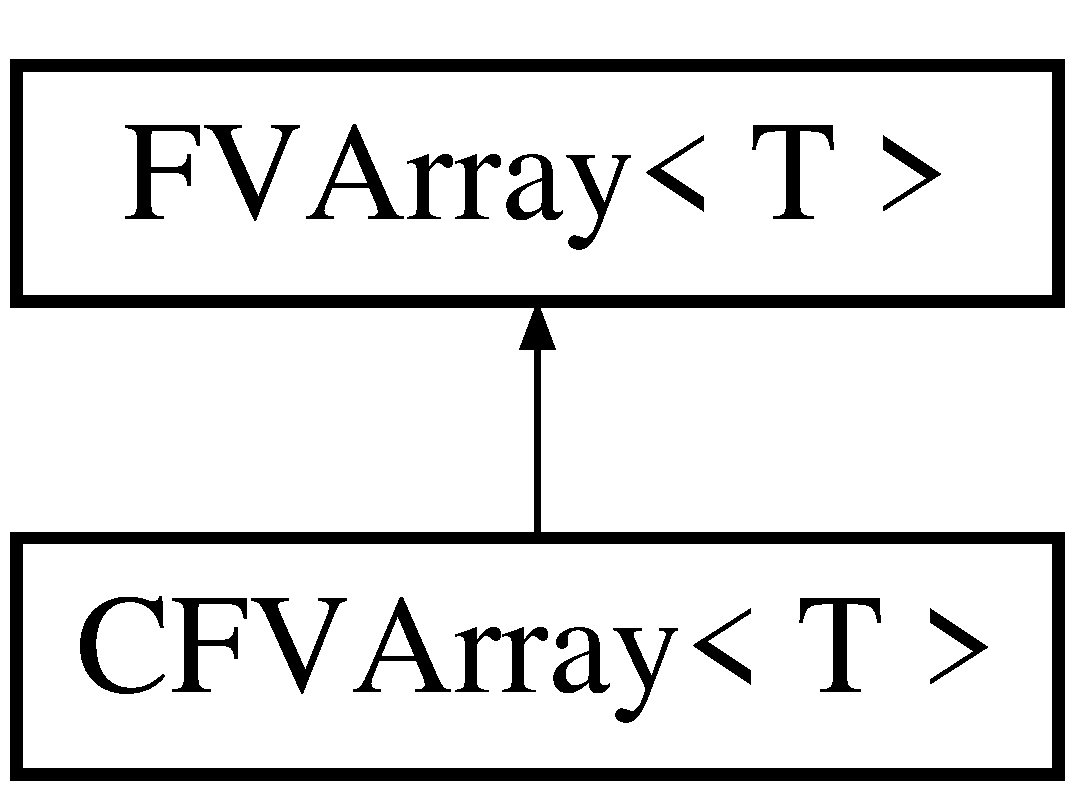
\includegraphics[height=2.000000cm]{dc/d80/classFVL_1_1CFVArray}
\end{center}
\end{figure}
\subsection*{Public Member Functions}
\begin{DoxyCompactItemize}
\item 
\hyperlink{classFVL_1_1CFVArray_af141a187a6f343f8f0acf258ee9428f5}{CFVArray} ()
\begin{DoxyCompactList}\small\item\em Empty constructor. \item\end{DoxyCompactList}\item 
\hyperlink{classFVL_1_1CFVArray_a4533252544513e80b44814b8afab3190}{CFVArray} (const unsigned int size)
\begin{DoxyCompactList}\small\item\em Constructor to create a CUDA-\/ready array with a given size. \item\end{DoxyCompactList}\item 
\hyperlink{classFVL_1_1CFVArray_a2bfe813d44db8292ff5793db73fe7fe0}{CFVArray} (const \hyperlink{classFVL_1_1CFVArray}{CFVArray}$<$ T $>$ \&copy)
\begin{DoxyCompactList}\small\item\em Constructor to create an array by copying an already existing array. \item\end{DoxyCompactList}\item 
\hyperlink{classFVL_1_1CFVArray_a3c7cfa5d9c6793cd2866030b734b5987}{$\sim$CFVArray} ()
\begin{DoxyCompactList}\small\item\em Default destructor. \item\end{DoxyCompactList}\item 
T $\ast$ \hyperlink{classFVL_1_1CFVArray_aa18ec3374bed8aae707bb943f500cb6f}{cuda\_\-get} ()
\begin{DoxyCompactList}\small\item\em Get pointer to CUDA memory of the array. \item\end{DoxyCompactList}\item 
T $\ast$ \hyperlink{classFVL_1_1CFVArray_af2915e0aeb48486f7210527178f3c1da}{cuda\_\-mallocAndSave} (cudaStream\_\-t stream=0)
\begin{DoxyCompactList}\small\item\em Allocates CUDA memory for the array, and copies data to it. \item\end{DoxyCompactList}\item 
T $\ast$ \hyperlink{classFVL_1_1CFVArray_ac5b54e1d7aacbc7ac8f947cc8403143e}{cuda\_\-malloc} ()
\begin{DoxyCompactList}\small\item\em Allocates CUDA memory for the array. \item\end{DoxyCompactList}\item 
void \hyperlink{classFVL_1_1CFVArray_a7da37a3af0dbb3b115a980bf13d30d02}{cuda\_\-free} ()
\begin{DoxyCompactList}\small\item\em Releases CUDA memory of this array. \item\end{DoxyCompactList}\item 
void \hyperlink{classFVL_1_1CFVArray_a817cca487c7f644b7e5d1abf8bd42308}{cuda\_\-save} (cudaStream\_\-t stream=0)
\begin{DoxyCompactList}\small\item\em Copies data from the array on host memory to CUDA memory. \item\end{DoxyCompactList}\item 
void \hyperlink{classFVL_1_1CFVArray_a9ea6b5a93cae1474a26ebef38d1eb350}{cuda\_\-load} (cudaStream\_\-t stream=0)
\begin{DoxyCompactList}\small\item\em Copies data from the array on CUDA memory back to the host. \item\end{DoxyCompactList}\end{DoxyCompactItemize}
\subsection*{Data Fields}
\begin{DoxyCompactItemize}
\item 
T $\ast$ \hyperlink{classFVL_1_1CFVArray_ac7c2eda2752dff79215dfcc062d0d814}{cuda\_\-arr}
\begin{DoxyCompactList}\small\item\em Ptr to CUDA memory of the array (NULL if not allocated). \item\end{DoxyCompactList}\end{DoxyCompactItemize}


\subsection{Detailed Description}
\subsubsection*{template$<$class T$>$ class FVL::CFVArray$<$ T $>$}

Generic CUDA-\/ready array template class. 

\subsection{Constructor \& Destructor Documentation}
\hypertarget{classFVL_1_1CFVArray_af141a187a6f343f8f0acf258ee9428f5}{
\index{FVL::CFVArray@{FVL::CFVArray}!CFVArray@{CFVArray}}
\index{CFVArray@{CFVArray}!FVL::CFVArray@{FVL::CFVArray}}
\subsubsection[{CFVArray}]{\setlength{\rightskip}{0pt plus 5cm}{\bf CFVArray} (
\begin{DoxyParamCaption}
{}
\end{DoxyParamCaption}
)\hspace{0.3cm}{\ttfamily  \mbox{[}inline\mbox{]}}}}
\label{dc/d80/classFVL_1_1CFVArray_af141a187a6f343f8f0acf258ee9428f5}


Empty constructor. 

\hypertarget{classFVL_1_1CFVArray_a4533252544513e80b44814b8afab3190}{
\index{FVL::CFVArray@{FVL::CFVArray}!CFVArray@{CFVArray}}
\index{CFVArray@{CFVArray}!FVL::CFVArray@{FVL::CFVArray}}
\subsubsection[{CFVArray}]{\setlength{\rightskip}{0pt plus 5cm}{\bf CFVArray} (
\begin{DoxyParamCaption}
\item[{const unsigned int}]{ size}
\end{DoxyParamCaption}
)\hspace{0.3cm}{\ttfamily  \mbox{[}inline\mbox{]}}}}
\label{dc/d80/classFVL_1_1CFVArray_a4533252544513e80b44814b8afab3190}


Constructor to create a CUDA-\/ready array with a given size. 


\begin{DoxyParams}{Parameters}
\item[{\em size}]Number of elements to allocate for the array \end{DoxyParams}
\hypertarget{classFVL_1_1CFVArray_a2bfe813d44db8292ff5793db73fe7fe0}{
\index{FVL::CFVArray@{FVL::CFVArray}!CFVArray@{CFVArray}}
\index{CFVArray@{CFVArray}!FVL::CFVArray@{FVL::CFVArray}}
\subsubsection[{CFVArray}]{\setlength{\rightskip}{0pt plus 5cm}{\bf CFVArray} (
\begin{DoxyParamCaption}
\item[{const {\bf CFVArray}$<$ T $>$ \&}]{ copy}
\end{DoxyParamCaption}
)\hspace{0.3cm}{\ttfamily  \mbox{[}inline\mbox{]}}}}
\label{dc/d80/classFVL_1_1CFVArray_a2bfe813d44db8292ff5793db73fe7fe0}


Constructor to create an array by copying an already existing array. 


\begin{DoxyParams}{Parameters}
\item[{\em copy}]Array to copy \end{DoxyParams}
\hypertarget{classFVL_1_1CFVArray_a3c7cfa5d9c6793cd2866030b734b5987}{
\index{FVL::CFVArray@{FVL::CFVArray}!$\sim$CFVArray@{$\sim$CFVArray}}
\index{$\sim$CFVArray@{$\sim$CFVArray}!FVL::CFVArray@{FVL::CFVArray}}
\subsubsection[{$\sim$CFVArray}]{\setlength{\rightskip}{0pt plus 5cm}$\sim${\bf CFVArray} (
\begin{DoxyParamCaption}
{}
\end{DoxyParamCaption}
)\hspace{0.3cm}{\ttfamily  \mbox{[}inline\mbox{]}}}}
\label{dc/d80/classFVL_1_1CFVArray_a3c7cfa5d9c6793cd2866030b734b5987}


Default destructor. 

Releases all memory allocated for this array 

\subsection{Member Function Documentation}
\hypertarget{classFVL_1_1CFVArray_a7da37a3af0dbb3b115a980bf13d30d02}{
\index{FVL::CFVArray@{FVL::CFVArray}!cuda\_\-free@{cuda\_\-free}}
\index{cuda\_\-free@{cuda\_\-free}!FVL::CFVArray@{FVL::CFVArray}}
\subsubsection[{cuda\_\-free}]{\setlength{\rightskip}{0pt plus 5cm}void cuda\_\-free (
\begin{DoxyParamCaption}
{}
\end{DoxyParamCaption}
)}}
\label{dc/d80/classFVL_1_1CFVArray_a7da37a3af0dbb3b115a980bf13d30d02}


Releases CUDA memory of this array. 

\hypertarget{classFVL_1_1CFVArray_aa18ec3374bed8aae707bb943f500cb6f}{
\index{FVL::CFVArray@{FVL::CFVArray}!cuda\_\-get@{cuda\_\-get}}
\index{cuda\_\-get@{cuda\_\-get}!FVL::CFVArray@{FVL::CFVArray}}
\subsubsection[{cuda\_\-get}]{\setlength{\rightskip}{0pt plus 5cm}T$\ast$ cuda\_\-get (
\begin{DoxyParamCaption}
{}
\end{DoxyParamCaption}
)}}
\label{dc/d80/classFVL_1_1CFVArray_aa18ec3374bed8aae707bb943f500cb6f}


Get pointer to CUDA memory of the array. 

\begin{DoxyReturn}{Returns}
Pointer to allocated memory on CUDA device (NULL if not allocated) 
\end{DoxyReturn}
\hypertarget{classFVL_1_1CFVArray_a9ea6b5a93cae1474a26ebef38d1eb350}{
\index{FVL::CFVArray@{FVL::CFVArray}!cuda\_\-load@{cuda\_\-load}}
\index{cuda\_\-load@{cuda\_\-load}!FVL::CFVArray@{FVL::CFVArray}}
\subsubsection[{cuda\_\-load}]{\setlength{\rightskip}{0pt plus 5cm}void cuda\_\-load (
\begin{DoxyParamCaption}
\item[{cudaStream\_\-t}]{ stream = {\ttfamily 0}}
\end{DoxyParamCaption}
)}}
\label{dc/d80/classFVL_1_1CFVArray_a9ea6b5a93cae1474a26ebef38d1eb350}


Copies data from the array on CUDA memory back to the host. 


\begin{DoxyParams}{Parameters}
\item[{\em stream}]CUDA Stream to use (defaults to 0 to use no stream) \end{DoxyParams}
\hypertarget{classFVL_1_1CFVArray_ac5b54e1d7aacbc7ac8f947cc8403143e}{
\index{FVL::CFVArray@{FVL::CFVArray}!cuda\_\-malloc@{cuda\_\-malloc}}
\index{cuda\_\-malloc@{cuda\_\-malloc}!FVL::CFVArray@{FVL::CFVArray}}
\subsubsection[{cuda\_\-malloc}]{\setlength{\rightskip}{0pt plus 5cm}T$\ast$ cuda\_\-malloc (
\begin{DoxyParamCaption}
{}
\end{DoxyParamCaption}
)}}
\label{dc/d80/classFVL_1_1CFVArray_ac5b54e1d7aacbc7ac8f947cc8403143e}


Allocates CUDA memory for the array. 

\begin{DoxyReturn}{Returns}
Pointer to allocated memory on CUDA device (NULL in case of allocation error) 
\end{DoxyReturn}
\hypertarget{classFVL_1_1CFVArray_af2915e0aeb48486f7210527178f3c1da}{
\index{FVL::CFVArray@{FVL::CFVArray}!cuda\_\-mallocAndSave@{cuda\_\-mallocAndSave}}
\index{cuda\_\-mallocAndSave@{cuda\_\-mallocAndSave}!FVL::CFVArray@{FVL::CFVArray}}
\subsubsection[{cuda\_\-mallocAndSave}]{\setlength{\rightskip}{0pt plus 5cm}T$\ast$ cuda\_\-mallocAndSave (
\begin{DoxyParamCaption}
\item[{cudaStream\_\-t}]{ stream = {\ttfamily 0}}
\end{DoxyParamCaption}
)}}
\label{dc/d80/classFVL_1_1CFVArray_af2915e0aeb48486f7210527178f3c1da}


Allocates CUDA memory for the array, and copies data to it. 

Equivalent to calling \hyperlink{classFVL_1_1CFVArray_ac5b54e1d7aacbc7ac8f947cc8403143e}{cuda\_\-malloc()} and \hyperlink{classFVL_1_1CFVArray_a817cca487c7f644b7e5d1abf8bd42308}{cuda\_\-save()} in sequence.


\begin{DoxyParams}{Parameters}
\item[{\em stream}]CUDA Stream to use (defaults to 0 to use no stream) \end{DoxyParams}
\begin{DoxyReturn}{Returns}
Pointer to allocated memory on CUDA device (NULL in case of allocation error) 
\end{DoxyReturn}
\hypertarget{classFVL_1_1CFVArray_a817cca487c7f644b7e5d1abf8bd42308}{
\index{FVL::CFVArray@{FVL::CFVArray}!cuda\_\-save@{cuda\_\-save}}
\index{cuda\_\-save@{cuda\_\-save}!FVL::CFVArray@{FVL::CFVArray}}
\subsubsection[{cuda\_\-save}]{\setlength{\rightskip}{0pt plus 5cm}void cuda\_\-save (
\begin{DoxyParamCaption}
\item[{cudaStream\_\-t}]{ stream = {\ttfamily 0}}
\end{DoxyParamCaption}
)}}
\label{dc/d80/classFVL_1_1CFVArray_a817cca487c7f644b7e5d1abf8bd42308}


Copies data from the array on host memory to CUDA memory. 


\begin{DoxyParams}{Parameters}
\item[{\em stream}]CUDA Stream to use (defaults to 0 to use no stream) \end{DoxyParams}


\subsection{Field Documentation}
\hypertarget{classFVL_1_1CFVArray_ac7c2eda2752dff79215dfcc062d0d814}{
\index{FVL::CFVArray@{FVL::CFVArray}!cuda\_\-arr@{cuda\_\-arr}}
\index{cuda\_\-arr@{cuda\_\-arr}!FVL::CFVArray@{FVL::CFVArray}}
\subsubsection[{cuda\_\-arr}]{\setlength{\rightskip}{0pt plus 5cm}T$\ast$ {\bf cuda\_\-arr}}}
\label{dc/d80/classFVL_1_1CFVArray_ac7c2eda2752dff79215dfcc062d0d814}


Ptr to CUDA memory of the array (NULL if not allocated). 



The documentation for this class was generated from the following file:\begin{DoxyCompactItemize}
\item 
include/FVL/\hyperlink{CFVArray_8h}{CFVArray.h}\end{DoxyCompactItemize}

\hypertarget{classFVL_1_1CFVMat}{
\section{CFVMat$<$ T $>$ Class Template Reference}
\label{d9/dcb/classFVL_1_1CFVMat}\index{FVL::CFVMat@{FVL::CFVMat}}
}


Generic CUDA-\/ready array of matrixes class.  




{\ttfamily \#include $<$CFVMat.h$>$}

\subsection*{Public Member Functions}
\begin{DoxyCompactItemize}
\item 
\hyperlink{classFVL_1_1CFVMat_a90b5cd38bfc076884d1f3cacc9f35cee}{CFVMat} (unsigned int w, unsigned int h, unsigned int size)
\begin{DoxyCompactList}\small\item\em Constructor to create a matrix with given dimensions. \item\end{DoxyCompactList}\item 
\hyperlink{classFVL_1_1CFVMat_a9746a1a3f248769a1268c2a225cedd52}{$\sim$CFVMat} ()
\begin{DoxyCompactList}\small\item\em Default destructor. \item\end{DoxyCompactList}\item 
\hyperlink{classFVL_1_1CFVArray}{CFVArray}$<$ T $>$ \& \hyperlink{classFVL_1_1CFVMat_ab179d788531c0f2d2f17e75896112f63}{elem} (unsigned int x, unsigned int y)
\begin{DoxyCompactList}\small\item\em Gives a vector of the matrix values at given coords. \item\end{DoxyCompactList}\item 
T \& \hyperlink{classFVL_1_1CFVMat_a2d02be460deeb3ad73a4bf0a3f9beb4d}{elem} (unsigned int x, unsigned int y, unsigned int i)
\begin{DoxyCompactList}\small\item\em Returns a single element of a matrix at given coordinates. \item\end{DoxyCompactList}\item 
vector$<$ \hyperlink{classFVL_1_1CFVArray}{CFVArray}$<$ T $>$ $>$ \& \hyperlink{classFVL_1_1CFVMat_a434d97b662d1620513d0f27ecd0e9b1e}{getMat} ()
\begin{DoxyCompactList}\small\item\em Get the vector of each array of the matrix. \item\end{DoxyCompactList}\item 
unsigned int \hyperlink{classFVL_1_1CFVMat_a90ca964ebcc1b02bbcde225edd49e812}{size} () const 
\begin{DoxyCompactList}\small\item\em Gives number of matrixes stored. \item\end{DoxyCompactList}\item 
unsigned int \hyperlink{classFVL_1_1CFVMat_a7b736ec9a05be5c498760d35a0406ed3}{width} () const 
\begin{DoxyCompactList}\small\item\em Gives width (number of columns) of each matrix. \item\end{DoxyCompactList}\item 
unsigned int \hyperlink{classFVL_1_1CFVMat_aa420a28166e708e3f8b9ecc8e527fc09}{height} () const 
\begin{DoxyCompactList}\small\item\em Gives height (number of rows) of each matrix. \item\end{DoxyCompactList}\item 
T $\ast$$\ast$ \hyperlink{classFVL_1_1CFVMat_a8b296b3ae7f031dac8aecc13b0bf39fc}{cuda\_\-get} ()
\begin{DoxyCompactList}\small\item\em Get the array of pointers for each elem in CUDA memory. \item\end{DoxyCompactList}\item 
T $\ast$$\ast$ \hyperlink{classFVL_1_1CFVMat_a09eadb0032c2862e02ddaf42732533f0}{cuda\_\-malloc} ()
\begin{DoxyCompactList}\small\item\em Allocates space in CUDA memory for all matrixes. \item\end{DoxyCompactList}\item 
T $\ast$$\ast$ \hyperlink{classFVL_1_1CFVMat_add6329cf5dda5b5bf602d724d6d69abc}{cuda\_\-mallocAndSave} (cudaStream\_\-t stream=0)
\begin{DoxyCompactList}\small\item\em Allocates space in CUDA memory for all matrixes, and copies all data to it. \item\end{DoxyCompactList}\item 
void \hyperlink{classFVL_1_1CFVMat_a7da37a3af0dbb3b115a980bf13d30d02}{cuda\_\-free} ()
\begin{DoxyCompactList}\small\item\em Releases CUDA memory of all matrixes. \item\end{DoxyCompactList}\item 
void \hyperlink{classFVL_1_1CFVMat_a817cca487c7f644b7e5d1abf8bd42308}{cuda\_\-save} (cudaStream\_\-t stream=0)
\begin{DoxyCompactList}\small\item\em copies data from the array on host memory to CUDA memory \item\end{DoxyCompactList}\item 
void \hyperlink{classFVL_1_1CFVMat_a9ea6b5a93cae1474a26ebef38d1eb350}{cuda\_\-load} (cudaStream\_\-t stream=0)
\begin{DoxyCompactList}\small\item\em copies data from the array on CUDA memory back to the host \item\end{DoxyCompactList}\end{DoxyCompactItemize}


\subsection{Detailed Description}
\subsubsection*{template$<$class T$>$ class FVL::CFVMat$<$ T $>$}

Generic CUDA-\/ready array of matrixes class. Even though it is meant to represent an array of matrixes, it is stored as a vector of arrays, where the vector is 1-\/dimensional representation of the 2D matrix.

Instead of accessing elements in the form mat\mbox{[}matrix\_\-index\mbox{]}\mbox{[}row\mbox{]}\mbox{[}column\mbox{]}, elements are accessed as mat\mbox{[}row $\ast$ width + column\mbox{]}\mbox{[}matrix\_\-index\mbox{]}. Method \hyperlink{classFVL_1_1CFVMat_ab179d788531c0f2d2f17e75896112f63}{elem()} provides an easier way of accessing items in CPU-\/code, in the form elem(row, column, matrix\_\-index)

\begin{Desc}
\item[\hyperlink{todo__todo000001}{Todo}]Allow for device-\/only allocation; alloc single block for whole matrix (allow single mem access instead of 2) \end{Desc}


\subsection{Constructor \& Destructor Documentation}
\hypertarget{classFVL_1_1CFVMat_a90b5cd38bfc076884d1f3cacc9f35cee}{
\index{FVL::CFVMat@{FVL::CFVMat}!CFVMat@{CFVMat}}
\index{CFVMat@{CFVMat}!FVL::CFVMat@{FVL::CFVMat}}
\subsubsection[{CFVMat}]{\setlength{\rightskip}{0pt plus 5cm}{\bf CFVMat} (
\begin{DoxyParamCaption}
\item[{unsigned int}]{ w, }
\item[{unsigned int}]{ h, }
\item[{unsigned int}]{ size}
\end{DoxyParamCaption}
)\hspace{0.3cm}{\ttfamily  \mbox{[}inline\mbox{]}}}}
\label{d9/dcb/classFVL_1_1CFVMat_a90b5cd38bfc076884d1f3cacc9f35cee}


Constructor to create a matrix with given dimensions. 


\begin{DoxyParams}{Parameters}
\item[{\em w}]Number of columns \item[{\em h}]Number of rows \item[{\em size}]Number of matrixes to allocated \end{DoxyParams}
\hypertarget{classFVL_1_1CFVMat_a9746a1a3f248769a1268c2a225cedd52}{
\index{FVL::CFVMat@{FVL::CFVMat}!$\sim$CFVMat@{$\sim$CFVMat}}
\index{$\sim$CFVMat@{$\sim$CFVMat}!FVL::CFVMat@{FVL::CFVMat}}
\subsubsection[{$\sim$CFVMat}]{\setlength{\rightskip}{0pt plus 5cm}$\sim${\bf CFVMat} (
\begin{DoxyParamCaption}
{}
\end{DoxyParamCaption}
)\hspace{0.3cm}{\ttfamily  \mbox{[}inline\mbox{]}}}}
\label{d9/dcb/classFVL_1_1CFVMat_a9746a1a3f248769a1268c2a225cedd52}


Default destructor. 

Releases all memory allocated for this array 

\subsection{Member Function Documentation}
\hypertarget{classFVL_1_1CFVMat_a7da37a3af0dbb3b115a980bf13d30d02}{
\index{FVL::CFVMat@{FVL::CFVMat}!cuda\_\-free@{cuda\_\-free}}
\index{cuda\_\-free@{cuda\_\-free}!FVL::CFVMat@{FVL::CFVMat}}
\subsubsection[{cuda\_\-free}]{\setlength{\rightskip}{0pt plus 5cm}void cuda\_\-free (
\begin{DoxyParamCaption}
{}
\end{DoxyParamCaption}
)}}
\label{d9/dcb/classFVL_1_1CFVMat_a7da37a3af0dbb3b115a980bf13d30d02}


Releases CUDA memory of all matrixes. 

\hypertarget{classFVL_1_1CFVMat_a8b296b3ae7f031dac8aecc13b0bf39fc}{
\index{FVL::CFVMat@{FVL::CFVMat}!cuda\_\-get@{cuda\_\-get}}
\index{cuda\_\-get@{cuda\_\-get}!FVL::CFVMat@{FVL::CFVMat}}
\subsubsection[{cuda\_\-get}]{\setlength{\rightskip}{0pt plus 5cm}T$\ast$$\ast$ cuda\_\-get (
\begin{DoxyParamCaption}
{}
\end{DoxyParamCaption}
)}}
\label{d9/dcb/classFVL_1_1CFVMat_a8b296b3ae7f031dac8aecc13b0bf39fc}


Get the array of pointers for each elem in CUDA memory. 

\begin{DoxyReturn}{Returns}
Array of pointers for each elem 
\end{DoxyReturn}
\hypertarget{classFVL_1_1CFVMat_a9ea6b5a93cae1474a26ebef38d1eb350}{
\index{FVL::CFVMat@{FVL::CFVMat}!cuda\_\-load@{cuda\_\-load}}
\index{cuda\_\-load@{cuda\_\-load}!FVL::CFVMat@{FVL::CFVMat}}
\subsubsection[{cuda\_\-load}]{\setlength{\rightskip}{0pt plus 5cm}void cuda\_\-load (
\begin{DoxyParamCaption}
\item[{cudaStream\_\-t}]{ stream = {\ttfamily 0}}
\end{DoxyParamCaption}
)}}
\label{d9/dcb/classFVL_1_1CFVMat_a9ea6b5a93cae1474a26ebef38d1eb350}


copies data from the array on CUDA memory back to the host 


\begin{DoxyParams}{Parameters}
\item[{\em stream}]cuda stream to use (defaults to 0 to use no stream) \end{DoxyParams}
\hypertarget{classFVL_1_1CFVMat_a09eadb0032c2862e02ddaf42732533f0}{
\index{FVL::CFVMat@{FVL::CFVMat}!cuda\_\-malloc@{cuda\_\-malloc}}
\index{cuda\_\-malloc@{cuda\_\-malloc}!FVL::CFVMat@{FVL::CFVMat}}
\subsubsection[{cuda\_\-malloc}]{\setlength{\rightskip}{0pt plus 5cm}T$\ast$$\ast$ cuda\_\-malloc (
\begin{DoxyParamCaption}
{}
\end{DoxyParamCaption}
)}}
\label{d9/dcb/classFVL_1_1CFVMat_a09eadb0032c2862e02ddaf42732533f0}


Allocates space in CUDA memory for all matrixes. 

\begin{DoxyReturn}{Returns}
Array of pointers for each elem 
\end{DoxyReturn}
\hypertarget{classFVL_1_1CFVMat_add6329cf5dda5b5bf602d724d6d69abc}{
\index{FVL::CFVMat@{FVL::CFVMat}!cuda\_\-mallocAndSave@{cuda\_\-mallocAndSave}}
\index{cuda\_\-mallocAndSave@{cuda\_\-mallocAndSave}!FVL::CFVMat@{FVL::CFVMat}}
\subsubsection[{cuda\_\-mallocAndSave}]{\setlength{\rightskip}{0pt plus 5cm}T$\ast$$\ast$ cuda\_\-mallocAndSave (
\begin{DoxyParamCaption}
\item[{cudaStream\_\-t}]{ stream = {\ttfamily 0}}
\end{DoxyParamCaption}
)}}
\label{d9/dcb/classFVL_1_1CFVMat_add6329cf5dda5b5bf602d724d6d69abc}


Allocates space in CUDA memory for all matrixes, and copies all data to it. 


\begin{DoxyParams}{Parameters}
\item[{\em stream}]CUDA Stream to use (defaults to 0 to use no stream) \end{DoxyParams}
\begin{DoxyReturn}{Returns}
Array of pointers for each elem 
\end{DoxyReturn}
\hypertarget{classFVL_1_1CFVMat_a817cca487c7f644b7e5d1abf8bd42308}{
\index{FVL::CFVMat@{FVL::CFVMat}!cuda\_\-save@{cuda\_\-save}}
\index{cuda\_\-save@{cuda\_\-save}!FVL::CFVMat@{FVL::CFVMat}}
\subsubsection[{cuda\_\-save}]{\setlength{\rightskip}{0pt plus 5cm}void cuda\_\-save (
\begin{DoxyParamCaption}
\item[{cudaStream\_\-t}]{ stream = {\ttfamily 0}}
\end{DoxyParamCaption}
)}}
\label{d9/dcb/classFVL_1_1CFVMat_a817cca487c7f644b7e5d1abf8bd42308}


copies data from the array on host memory to CUDA memory 


\begin{DoxyParams}{Parameters}
\item[{\em stream}]cuda stream to use (defaults to 0 to use no stream) \end{DoxyParams}
\hypertarget{classFVL_1_1CFVMat_a2d02be460deeb3ad73a4bf0a3f9beb4d}{
\index{FVL::CFVMat@{FVL::CFVMat}!elem@{elem}}
\index{elem@{elem}!FVL::CFVMat@{FVL::CFVMat}}
\subsubsection[{elem}]{\setlength{\rightskip}{0pt plus 5cm}T\& elem (
\begin{DoxyParamCaption}
\item[{unsigned int}]{ x, }
\item[{unsigned int}]{ y, }
\item[{unsigned int}]{ i}
\end{DoxyParamCaption}
)\hspace{0.3cm}{\ttfamily  \mbox{[}inline\mbox{]}}}}
\label{d9/dcb/classFVL_1_1CFVMat_a2d02be460deeb3ad73a4bf0a3f9beb4d}


Returns a single element of a matrix at given coordinates. 


\begin{DoxyParams}{Parameters}
\item[{\em x}]Row of the element to acess \item[{\em y}]Column of the element to access \item[{\em i}]Index of the matrix to acess \end{DoxyParams}
\begin{DoxyReturn}{Returns}
element of matrix with index i, at coordinates (x, y) 
\end{DoxyReturn}
\hypertarget{classFVL_1_1CFVMat_ab179d788531c0f2d2f17e75896112f63}{
\index{FVL::CFVMat@{FVL::CFVMat}!elem@{elem}}
\index{elem@{elem}!FVL::CFVMat@{FVL::CFVMat}}
\subsubsection[{elem}]{\setlength{\rightskip}{0pt plus 5cm}{\bf CFVArray}$<$T$>$\& elem (
\begin{DoxyParamCaption}
\item[{unsigned int}]{ x, }
\item[{unsigned int}]{ y}
\end{DoxyParamCaption}
)\hspace{0.3cm}{\ttfamily  \mbox{[}inline\mbox{]}}}}
\label{d9/dcb/classFVL_1_1CFVMat_ab179d788531c0f2d2f17e75896112f63}


Gives a vector of the matrix values at given coords. 

For coords (x, y) gives the vector with elements of each matrix at position (x, y)


\begin{DoxyParams}{Parameters}
\item[{\em x}]Row of the matrixes to access \item[{\em y}]Column of the matrixes to access \end{DoxyParams}
\begin{DoxyReturn}{Returns}
Array of elements contained at (x, y) in each matrix 
\end{DoxyReturn}
\hypertarget{classFVL_1_1CFVMat_a434d97b662d1620513d0f27ecd0e9b1e}{
\index{FVL::CFVMat@{FVL::CFVMat}!getMat@{getMat}}
\index{getMat@{getMat}!FVL::CFVMat@{FVL::CFVMat}}
\subsubsection[{getMat}]{\setlength{\rightskip}{0pt plus 5cm}vector$<${\bf CFVArray}$<$T$>$ $>$\& getMat (
\begin{DoxyParamCaption}
{}
\end{DoxyParamCaption}
)\hspace{0.3cm}{\ttfamily  \mbox{[}inline\mbox{]}}}}
\label{d9/dcb/classFVL_1_1CFVMat_a434d97b662d1620513d0f27ecd0e9b1e}


Get the vector of each array of the matrix. 

\begin{DoxyReturn}{Returns}
Vector of arrays of the matrix 
\end{DoxyReturn}
\hypertarget{classFVL_1_1CFVMat_aa420a28166e708e3f8b9ecc8e527fc09}{
\index{FVL::CFVMat@{FVL::CFVMat}!height@{height}}
\index{height@{height}!FVL::CFVMat@{FVL::CFVMat}}
\subsubsection[{height}]{\setlength{\rightskip}{0pt plus 5cm}unsigned int height (
\begin{DoxyParamCaption}
{}
\end{DoxyParamCaption}
) const\hspace{0.3cm}{\ttfamily  \mbox{[}inline\mbox{]}}}}
\label{d9/dcb/classFVL_1_1CFVMat_aa420a28166e708e3f8b9ecc8e527fc09}


Gives height (number of rows) of each matrix. 

\begin{DoxyReturn}{Returns}
Height of each matrix 
\end{DoxyReturn}
\hypertarget{classFVL_1_1CFVMat_a90ca964ebcc1b02bbcde225edd49e812}{
\index{FVL::CFVMat@{FVL::CFVMat}!size@{size}}
\index{size@{size}!FVL::CFVMat@{FVL::CFVMat}}
\subsubsection[{size}]{\setlength{\rightskip}{0pt plus 5cm}unsigned int size (
\begin{DoxyParamCaption}
{}
\end{DoxyParamCaption}
) const\hspace{0.3cm}{\ttfamily  \mbox{[}inline\mbox{]}}}}
\label{d9/dcb/classFVL_1_1CFVMat_a90ca964ebcc1b02bbcde225edd49e812}


Gives number of matrixes stored. 

\begin{DoxyReturn}{Returns}
Number of matrixes stored 
\end{DoxyReturn}
\hypertarget{classFVL_1_1CFVMat_a7b736ec9a05be5c498760d35a0406ed3}{
\index{FVL::CFVMat@{FVL::CFVMat}!width@{width}}
\index{width@{width}!FVL::CFVMat@{FVL::CFVMat}}
\subsubsection[{width}]{\setlength{\rightskip}{0pt plus 5cm}unsigned int width (
\begin{DoxyParamCaption}
{}
\end{DoxyParamCaption}
) const\hspace{0.3cm}{\ttfamily  \mbox{[}inline\mbox{]}}}}
\label{d9/dcb/classFVL_1_1CFVMat_a7b736ec9a05be5c498760d35a0406ed3}


Gives width (number of columns) of each matrix. 

\begin{DoxyReturn}{Returns}
Width of each matrix 
\end{DoxyReturn}


The documentation for this class was generated from the following file:\begin{DoxyCompactItemize}
\item 
include/FVL/\hyperlink{CFVMat_8h}{CFVMat.h}\end{DoxyCompactItemize}

\hypertarget{classFVL_1_1CFVMesh2D}{
\section{CFVMesh2D Class Reference}
\label{da/d8d/classFVL_1_1CFVMesh2D}\index{FVL::CFVMesh2D@{FVL::CFVMesh2D}}
}


A CUDA enabled 2D Mesh.  




{\ttfamily \#include $<$CFVMesh2D.h$>$}

\subsection*{Public Member Functions}
\begin{DoxyCompactItemize}
\item 
\hyperlink{classFVL_1_1CFVMesh2D_aa7a00d0164463a128c305eff51e3218d}{CFVMesh2D} (\hyperlink{classFVMesh2D}{FVMesh2D} \&msh)
\begin{DoxyCompactList}\small\item\em Constructor to import a mesh on original \hyperlink{classFVMesh2D}{FVMesh2D} format. \item\end{DoxyCompactList}\item 
\hyperlink{classFVL_1_1CFVMesh2D_a1cac005d50e5d1ed3d3a279bded6560c}{CFVMesh2D} (const string \&filename)
\begin{DoxyCompactList}\small\item\em Constructor to import a mesh from a XML file. \item\end{DoxyCompactList}\item 
\hyperlink{classFVL_1_1CFVMesh2D_a1e8707cd63592ebc0debed957fb072e9}{$\sim$CFVMesh2D} ()
\begin{DoxyCompactList}\small\item\em Default destructor. \item\end{DoxyCompactList}\item 
\hyperlink{structFVL_1_1CFVMesh2D__cuda}{CFVMesh2D\_\-cuda} $\ast$ \hyperlink{classFVL_1_1CFVMesh2D_af4e692bafdba2014d215f7a7ba2bdc3a}{cuda\_\-get} ()
\begin{DoxyCompactList}\small\item\em Returns a pointer to device memory containing the mesh in CFVMesh2D\_\-cuda format. \item\end{DoxyCompactList}\item 
bool \hyperlink{classFVL_1_1CFVMesh2D_af451f67501054350bf2009f98ed5fe11}{cuda\_\-is\_\-alloc} ()
\begin{DoxyCompactList}\small\item\em Checks whether device memory is allocated. \item\end{DoxyCompactList}\item 
\hyperlink{structFVL_1_1CFVMesh2D__cuda}{CFVMesh2D\_\-cuda} $\ast$ \hyperlink{classFVL_1_1CFVMesh2D_aa84c3c881bec148d68a3e847feb4ecd5}{cuda\_\-malloc} ()
\begin{DoxyCompactList}\small\item\em Allocate space on device memory for the entire mesh. \item\end{DoxyCompactList}\item 
void \hyperlink{classFVL_1_1CFVMesh2D_a817cca487c7f644b7e5d1abf8bd42308}{cuda\_\-save} (cudaStream\_\-t stream=0)
\begin{DoxyCompactList}\small\item\em Saves entire mesh to cuda memory. \item\end{DoxyCompactList}\item 
void \hyperlink{classFVL_1_1CFVMesh2D_a7da37a3af0dbb3b115a980bf13d30d02}{cuda\_\-free} ()
\begin{DoxyCompactList}\small\item\em Free all cuda storage of this mesh. \item\end{DoxyCompactList}\end{DoxyCompactItemize}
\subsection*{Data Fields}
\begin{DoxyCompactItemize}
\item 
unsigned int \hyperlink{classFVL_1_1CFVMesh2D_a66b841fd6e58a9fc9b63df4fe982178f}{num\_\-vertex}
\begin{DoxyCompactList}\small\item\em total number of vertex \item\end{DoxyCompactList}\item 
\hyperlink{classFVL_1_1CFVPoints2D}{CFVPoints2D}$<$ double $>$ \hyperlink{classFVL_1_1CFVMesh2D_a87d5c74a26438af8208b9ee9fe5608d5}{vertex\_\-coords}
\begin{DoxyCompactList}\small\item\em coords for each vertex \item\end{DoxyCompactList}\item 
unsigned int \hyperlink{classFVL_1_1CFVMesh2D_ad1228ae08a3c287de40e4682e6538c12}{num\_\-edges}
\begin{DoxyCompactList}\small\item\em total number of edges \item\end{DoxyCompactList}\item 
\hyperlink{classFVL_1_1CFVArray}{CFVArray}$<$ int $>$ \hyperlink{classFVL_1_1CFVMesh2D_a8ea0de28dab4c5c3326c8b25b836b8e0}{edge\_\-types}
\begin{DoxyCompactList}\small\item\em type associated with each edge \item\end{DoxyCompactList}\item 
\hyperlink{classFVL_1_1CFVPoints2D}{CFVPoints2D}$<$ double $>$ \hyperlink{classFVL_1_1CFVMesh2D_a42a15adf693b0a6b35f542a7eebd51ed}{edge\_\-normals}
\begin{DoxyCompactList}\small\item\em normals for each edge \item\end{DoxyCompactList}\item 
\hyperlink{classFVL_1_1CFVPoints2D}{CFVPoints2D}$<$ double $>$ \hyperlink{classFVL_1_1CFVMesh2D_a3d6b698a768743ed6a78ab1603146522}{edge\_\-centroids}
\begin{DoxyCompactList}\small\item\em centroid for each edge \item\end{DoxyCompactList}\item 
\hyperlink{classFVL_1_1CFVArray}{CFVArray}$<$ double $>$ \hyperlink{classFVL_1_1CFVMesh2D_aebae766e252c936bed264b8ff3c9523d}{edge\_\-lengths}
\begin{DoxyCompactList}\small\item\em length for each edge \item\end{DoxyCompactList}\item 
\hyperlink{classFVL_1_1CFVArray}{CFVArray}$<$ unsigned int $>$ \hyperlink{classFVL_1_1CFVMesh2D_a21b745a28be501c6f6e79d4cef3ef779}{edge\_\-fst\_\-vertex}
\begin{DoxyCompactList}\small\item\em first vertex of each edge \item\end{DoxyCompactList}\item 
\hyperlink{classFVL_1_1CFVArray}{CFVArray}$<$ unsigned int $>$ \hyperlink{classFVL_1_1CFVMesh2D_a68d5bdf0974c1e9c24b511c6e3801664}{edge\_\-snd\_\-vertex}
\begin{DoxyCompactList}\small\item\em second vertex of each edge \item\end{DoxyCompactList}\item 
\hyperlink{classFVL_1_1CFVArray}{CFVArray}$<$ unsigned int $>$ \hyperlink{classFVL_1_1CFVMesh2D_a9fc942016b70da68970d941850fc4328}{edge\_\-left\_\-cells}
\begin{DoxyCompactList}\small\item\em left cell of each edge \item\end{DoxyCompactList}\item 
\hyperlink{classFVL_1_1CFVArray}{CFVArray}$<$ unsigned int $>$ \hyperlink{classFVL_1_1CFVMesh2D_a99a2c529d96512148f33c07cae218825}{edge\_\-right\_\-cells}
\begin{DoxyCompactList}\small\item\em right cell of each edge (NO\_\-RIGHT\_\-CELL indicates a border edge where no right cell exists) \item\end{DoxyCompactList}\item 
unsigned int \hyperlink{classFVL_1_1CFVMesh2D_aede6f897b05f909a426f36f61b2b8d43}{num\_\-cells}
\begin{DoxyCompactList}\small\item\em total number of cells \item\end{DoxyCompactList}\item 
\hyperlink{classFVL_1_1CFVArray}{CFVArray}$<$ int $>$ \hyperlink{classFVL_1_1CFVMesh2D_a373a520b2d4015b9602a58759dcd39cd}{cell\_\-types}
\begin{DoxyCompactList}\small\item\em type associated with each cell \item\end{DoxyCompactList}\item 
\hyperlink{classFVL_1_1CFVPoints2D}{CFVPoints2D}$<$ double $>$ \hyperlink{classFVL_1_1CFVMesh2D_a63792291626ccfe6bdf93b3904a8320b}{cell\_\-centroids}
\begin{DoxyCompactList}\small\item\em centroid for each cell \item\end{DoxyCompactList}\item 
\hyperlink{classFVL_1_1CFVArray}{CFVArray}$<$ double $>$ \hyperlink{classFVL_1_1CFVMesh2D_a9b0f6ae0e30a2b7dedfeba13d4590fe3}{cell\_\-perimeters}
\begin{DoxyCompactList}\small\item\em perimeter for each cell \item\end{DoxyCompactList}\item 
\hyperlink{classFVL_1_1CFVArray}{CFVArray}$<$ double $>$ \hyperlink{classFVL_1_1CFVMesh2D_a012b4e69e4350c5c1e61394ba875f8d4}{cell\_\-areas}
\begin{DoxyCompactList}\small\item\em area for each cell \item\end{DoxyCompactList}\item 
\hyperlink{classFVL_1_1CFVArray}{CFVArray}$<$ unsigned int $>$ \hyperlink{classFVL_1_1CFVMesh2D_ac40c328fe38b4afc77363050e278bcce}{cell\_\-edges\_\-count}
\begin{DoxyCompactList}\small\item\em number of edges of each cell (to index cell\_\-edges) \item\end{DoxyCompactList}\item 
\hyperlink{classFVL_1_1CFVMat}{CFVMat}$<$ unsigned int $>$ \hyperlink{classFVL_1_1CFVMesh2D_a088a198cb26befce9c0f1cab67e00705}{cell\_\-edges}
\begin{DoxyCompactList}\small\item\em index of edges for each cell (CFVMat(MAX\_\-EDGES\_\-PER\_\-CELL, 1, num\_\-cells) \item\end{DoxyCompactList}\item 
\hyperlink{classFVL_1_1CFVMat}{CFVMat}$<$ double $>$ \hyperlink{classFVL_1_1CFVMesh2D_a1dc398446290133710b75ca776d4abda}{cell\_\-edges\_\-normal}
\begin{DoxyCompactList}\small\item\em distance of each cell to each edge (CFVMat(MAX\_\-EDGES\_\-PER\_\-CELL, 2, num\_\-cells) \item\end{DoxyCompactList}\end{DoxyCompactItemize}


\subsection{Detailed Description}
A CUDA enabled 2D Mesh. 2 Dimensional mesh representation using Structure of Arrays instead of Array of Structures 

\subsection{Constructor \& Destructor Documentation}
\hypertarget{classFVL_1_1CFVMesh2D_aa7a00d0164463a128c305eff51e3218d}{
\index{FVL::CFVMesh2D@{FVL::CFVMesh2D}!CFVMesh2D@{CFVMesh2D}}
\index{CFVMesh2D@{CFVMesh2D}!FVL::CFVMesh2D@{FVL::CFVMesh2D}}
\subsubsection[{CFVMesh2D}]{\setlength{\rightskip}{0pt plus 5cm}{\bf CFVMesh2D} (
\begin{DoxyParamCaption}
\item[{{\bf FVMesh2D} \&}]{ msh}
\end{DoxyParamCaption}
)}}
\label{da/d8d/classFVL_1_1CFVMesh2D_aa7a00d0164463a128c305eff51e3218d}


Constructor to import a mesh on original \hyperlink{classFVMesh2D}{FVMesh2D} format. 


\begin{DoxyParams}{Parameters}
\item[{\em msh}]Mesh to import \end{DoxyParams}
\hypertarget{classFVL_1_1CFVMesh2D_a1cac005d50e5d1ed3d3a279bded6560c}{
\index{FVL::CFVMesh2D@{FVL::CFVMesh2D}!CFVMesh2D@{CFVMesh2D}}
\index{CFVMesh2D@{CFVMesh2D}!FVL::CFVMesh2D@{FVL::CFVMesh2D}}
\subsubsection[{CFVMesh2D}]{\setlength{\rightskip}{0pt plus 5cm}{\bf CFVMesh2D} (
\begin{DoxyParamCaption}
\item[{const string \&}]{ filename}
\end{DoxyParamCaption}
)}}
\label{da/d8d/classFVL_1_1CFVMesh2D_a1cac005d50e5d1ed3d3a279bded6560c}


Constructor to import a mesh from a XML file. 


\begin{DoxyParams}{Parameters}
\item[{\em filename}]XML file to import \end{DoxyParams}
\hypertarget{classFVL_1_1CFVMesh2D_a1e8707cd63592ebc0debed957fb072e9}{
\index{FVL::CFVMesh2D@{FVL::CFVMesh2D}!$\sim$CFVMesh2D@{$\sim$CFVMesh2D}}
\index{$\sim$CFVMesh2D@{$\sim$CFVMesh2D}!FVL::CFVMesh2D@{FVL::CFVMesh2D}}
\subsubsection[{$\sim$CFVMesh2D}]{\setlength{\rightskip}{0pt plus 5cm}$\sim${\bf CFVMesh2D} (
\begin{DoxyParamCaption}
{}
\end{DoxyParamCaption}
)}}
\label{da/d8d/classFVL_1_1CFVMesh2D_a1e8707cd63592ebc0debed957fb072e9}


Default destructor. 

Releases all memory allocated by the mesh, both on host and device 

\subsection{Member Function Documentation}
\hypertarget{classFVL_1_1CFVMesh2D_a7da37a3af0dbb3b115a980bf13d30d02}{
\index{FVL::CFVMesh2D@{FVL::CFVMesh2D}!cuda\_\-free@{cuda\_\-free}}
\index{cuda\_\-free@{cuda\_\-free}!FVL::CFVMesh2D@{FVL::CFVMesh2D}}
\subsubsection[{cuda\_\-free}]{\setlength{\rightskip}{0pt plus 5cm}void cuda\_\-free (
\begin{DoxyParamCaption}
{}
\end{DoxyParamCaption}
)}}
\label{da/d8d/classFVL_1_1CFVMesh2D_a7da37a3af0dbb3b115a980bf13d30d02}


Free all cuda storage of this mesh. 

\hypertarget{classFVL_1_1CFVMesh2D_af4e692bafdba2014d215f7a7ba2bdc3a}{
\index{FVL::CFVMesh2D@{FVL::CFVMesh2D}!cuda\_\-get@{cuda\_\-get}}
\index{cuda\_\-get@{cuda\_\-get}!FVL::CFVMesh2D@{FVL::CFVMesh2D}}
\subsubsection[{cuda\_\-get}]{\setlength{\rightskip}{0pt plus 5cm}{\bf CFVMesh2D\_\-cuda}$\ast$ cuda\_\-get (
\begin{DoxyParamCaption}
{}
\end{DoxyParamCaption}
)}}
\label{da/d8d/classFVL_1_1CFVMesh2D_af4e692bafdba2014d215f7a7ba2bdc3a}


Returns a pointer to device memory containing the mesh in CFVMesh2D\_\-cuda format. 

If device memory is already allocated, nothing is done, and the current pointer is returned unaltered. Use \hyperlink{classFVL_1_1CFVMesh2D_a7da37a3af0dbb3b115a980bf13d30d02}{cuda\_\-free()} first to force mesh reallocation.

\begin{DoxyReturn}{Returns}
Pointer to CFVMesh2D\_\-cuda struct, or NULL if no memory was previously allocated on the device 
\end{DoxyReturn}
\hypertarget{classFVL_1_1CFVMesh2D_af451f67501054350bf2009f98ed5fe11}{
\index{FVL::CFVMesh2D@{FVL::CFVMesh2D}!cuda\_\-is\_\-alloc@{cuda\_\-is\_\-alloc}}
\index{cuda\_\-is\_\-alloc@{cuda\_\-is\_\-alloc}!FVL::CFVMesh2D@{FVL::CFVMesh2D}}
\subsubsection[{cuda\_\-is\_\-alloc}]{\setlength{\rightskip}{0pt plus 5cm}bool cuda\_\-is\_\-alloc (
\begin{DoxyParamCaption}
{}
\end{DoxyParamCaption}
)}}
\label{da/d8d/classFVL_1_1CFVMesh2D_af451f67501054350bf2009f98ed5fe11}


Checks whether device memory is allocated. 

\begin{DoxyReturn}{Returns}
true if memory is allocated on the CUDA device, false otherwise 
\end{DoxyReturn}
\hypertarget{classFVL_1_1CFVMesh2D_aa84c3c881bec148d68a3e847feb4ecd5}{
\index{FVL::CFVMesh2D@{FVL::CFVMesh2D}!cuda\_\-malloc@{cuda\_\-malloc}}
\index{cuda\_\-malloc@{cuda\_\-malloc}!FVL::CFVMesh2D@{FVL::CFVMesh2D}}
\subsubsection[{cuda\_\-malloc}]{\setlength{\rightskip}{0pt plus 5cm}{\bf CFVMesh2D\_\-cuda}$\ast$ cuda\_\-malloc (
\begin{DoxyParamCaption}
{}
\end{DoxyParamCaption}
)}}
\label{da/d8d/classFVL_1_1CFVMesh2D_aa84c3c881bec148d68a3e847feb4ecd5}


Allocate space on device memory for the entire mesh. 

\begin{DoxyReturn}{Returns}
Ptr to CFVMesh2D\_\-cuda structure where all data is stored 
\end{DoxyReturn}
\hypertarget{classFVL_1_1CFVMesh2D_a817cca487c7f644b7e5d1abf8bd42308}{
\index{FVL::CFVMesh2D@{FVL::CFVMesh2D}!cuda\_\-save@{cuda\_\-save}}
\index{cuda\_\-save@{cuda\_\-save}!FVL::CFVMesh2D@{FVL::CFVMesh2D}}
\subsubsection[{cuda\_\-save}]{\setlength{\rightskip}{0pt plus 5cm}void cuda\_\-save (
\begin{DoxyParamCaption}
\item[{cudaStream\_\-t}]{ stream = {\ttfamily 0}}
\end{DoxyParamCaption}
)}}
\label{da/d8d/classFVL_1_1CFVMesh2D_a817cca487c7f644b7e5d1abf8bd42308}


Saves entire mesh to cuda memory. 

Memory must have been previously allocated with \hyperlink{classFVL_1_1CFVMesh2D_aa84c3c881bec148d68a3e847feb4ecd5}{cuda\_\-malloc()}


\begin{DoxyParams}{Parameters}
\item[{\em stream}]CUDA Stream to use (defaults to 0 to use no stream) \end{DoxyParams}


\subsection{Field Documentation}
\hypertarget{classFVL_1_1CFVMesh2D_a012b4e69e4350c5c1e61394ba875f8d4}{
\index{FVL::CFVMesh2D@{FVL::CFVMesh2D}!cell\_\-areas@{cell\_\-areas}}
\index{cell\_\-areas@{cell\_\-areas}!FVL::CFVMesh2D@{FVL::CFVMesh2D}}
\subsubsection[{cell\_\-areas}]{\setlength{\rightskip}{0pt plus 5cm}{\bf CFVArray}$<$double$>$ {\bf cell\_\-areas}}}
\label{da/d8d/classFVL_1_1CFVMesh2D_a012b4e69e4350c5c1e61394ba875f8d4}


area for each cell 

\hypertarget{classFVL_1_1CFVMesh2D_a63792291626ccfe6bdf93b3904a8320b}{
\index{FVL::CFVMesh2D@{FVL::CFVMesh2D}!cell\_\-centroids@{cell\_\-centroids}}
\index{cell\_\-centroids@{cell\_\-centroids}!FVL::CFVMesh2D@{FVL::CFVMesh2D}}
\subsubsection[{cell\_\-centroids}]{\setlength{\rightskip}{0pt plus 5cm}{\bf CFVPoints2D}$<$double$>$ {\bf cell\_\-centroids}}}
\label{da/d8d/classFVL_1_1CFVMesh2D_a63792291626ccfe6bdf93b3904a8320b}


centroid for each cell 

\hypertarget{classFVL_1_1CFVMesh2D_a088a198cb26befce9c0f1cab67e00705}{
\index{FVL::CFVMesh2D@{FVL::CFVMesh2D}!cell\_\-edges@{cell\_\-edges}}
\index{cell\_\-edges@{cell\_\-edges}!FVL::CFVMesh2D@{FVL::CFVMesh2D}}
\subsubsection[{cell\_\-edges}]{\setlength{\rightskip}{0pt plus 5cm}{\bf CFVMat}$<$unsigned int$>$ {\bf cell\_\-edges}}}
\label{da/d8d/classFVL_1_1CFVMesh2D_a088a198cb26befce9c0f1cab67e00705}


index of edges for each cell (CFVMat(MAX\_\-EDGES\_\-PER\_\-CELL, 1, num\_\-cells) 

\hypertarget{classFVL_1_1CFVMesh2D_ac40c328fe38b4afc77363050e278bcce}{
\index{FVL::CFVMesh2D@{FVL::CFVMesh2D}!cell\_\-edges\_\-count@{cell\_\-edges\_\-count}}
\index{cell\_\-edges\_\-count@{cell\_\-edges\_\-count}!FVL::CFVMesh2D@{FVL::CFVMesh2D}}
\subsubsection[{cell\_\-edges\_\-count}]{\setlength{\rightskip}{0pt plus 5cm}{\bf CFVArray}$<$unsigned int$>$ {\bf cell\_\-edges\_\-count}}}
\label{da/d8d/classFVL_1_1CFVMesh2D_ac40c328fe38b4afc77363050e278bcce}


number of edges of each cell (to index cell\_\-edges) 

\hypertarget{classFVL_1_1CFVMesh2D_a1dc398446290133710b75ca776d4abda}{
\index{FVL::CFVMesh2D@{FVL::CFVMesh2D}!cell\_\-edges\_\-normal@{cell\_\-edges\_\-normal}}
\index{cell\_\-edges\_\-normal@{cell\_\-edges\_\-normal}!FVL::CFVMesh2D@{FVL::CFVMesh2D}}
\subsubsection[{cell\_\-edges\_\-normal}]{\setlength{\rightskip}{0pt plus 5cm}{\bf CFVMat}$<$double$>$ {\bf cell\_\-edges\_\-normal}}}
\label{da/d8d/classFVL_1_1CFVMesh2D_a1dc398446290133710b75ca776d4abda}


distance of each cell to each edge (CFVMat(MAX\_\-EDGES\_\-PER\_\-CELL, 2, num\_\-cells) 

\hypertarget{classFVL_1_1CFVMesh2D_a9b0f6ae0e30a2b7dedfeba13d4590fe3}{
\index{FVL::CFVMesh2D@{FVL::CFVMesh2D}!cell\_\-perimeters@{cell\_\-perimeters}}
\index{cell\_\-perimeters@{cell\_\-perimeters}!FVL::CFVMesh2D@{FVL::CFVMesh2D}}
\subsubsection[{cell\_\-perimeters}]{\setlength{\rightskip}{0pt plus 5cm}{\bf CFVArray}$<$double$>$ {\bf cell\_\-perimeters}}}
\label{da/d8d/classFVL_1_1CFVMesh2D_a9b0f6ae0e30a2b7dedfeba13d4590fe3}


perimeter for each cell 

\hypertarget{classFVL_1_1CFVMesh2D_a373a520b2d4015b9602a58759dcd39cd}{
\index{FVL::CFVMesh2D@{FVL::CFVMesh2D}!cell\_\-types@{cell\_\-types}}
\index{cell\_\-types@{cell\_\-types}!FVL::CFVMesh2D@{FVL::CFVMesh2D}}
\subsubsection[{cell\_\-types}]{\setlength{\rightskip}{0pt plus 5cm}{\bf CFVArray}$<$int$>$ {\bf cell\_\-types}}}
\label{da/d8d/classFVL_1_1CFVMesh2D_a373a520b2d4015b9602a58759dcd39cd}


type associated with each cell 

\hypertarget{classFVL_1_1CFVMesh2D_a3d6b698a768743ed6a78ab1603146522}{
\index{FVL::CFVMesh2D@{FVL::CFVMesh2D}!edge\_\-centroids@{edge\_\-centroids}}
\index{edge\_\-centroids@{edge\_\-centroids}!FVL::CFVMesh2D@{FVL::CFVMesh2D}}
\subsubsection[{edge\_\-centroids}]{\setlength{\rightskip}{0pt plus 5cm}{\bf CFVPoints2D}$<$double$>$ {\bf edge\_\-centroids}}}
\label{da/d8d/classFVL_1_1CFVMesh2D_a3d6b698a768743ed6a78ab1603146522}


centroid for each edge 

\hypertarget{classFVL_1_1CFVMesh2D_a21b745a28be501c6f6e79d4cef3ef779}{
\index{FVL::CFVMesh2D@{FVL::CFVMesh2D}!edge\_\-fst\_\-vertex@{edge\_\-fst\_\-vertex}}
\index{edge\_\-fst\_\-vertex@{edge\_\-fst\_\-vertex}!FVL::CFVMesh2D@{FVL::CFVMesh2D}}
\subsubsection[{edge\_\-fst\_\-vertex}]{\setlength{\rightskip}{0pt plus 5cm}{\bf CFVArray}$<$unsigned int$>$ {\bf edge\_\-fst\_\-vertex}}}
\label{da/d8d/classFVL_1_1CFVMesh2D_a21b745a28be501c6f6e79d4cef3ef779}


first vertex of each edge 

\hypertarget{classFVL_1_1CFVMesh2D_a9fc942016b70da68970d941850fc4328}{
\index{FVL::CFVMesh2D@{FVL::CFVMesh2D}!edge\_\-left\_\-cells@{edge\_\-left\_\-cells}}
\index{edge\_\-left\_\-cells@{edge\_\-left\_\-cells}!FVL::CFVMesh2D@{FVL::CFVMesh2D}}
\subsubsection[{edge\_\-left\_\-cells}]{\setlength{\rightskip}{0pt plus 5cm}{\bf CFVArray}$<$unsigned int$>$ {\bf edge\_\-left\_\-cells}}}
\label{da/d8d/classFVL_1_1CFVMesh2D_a9fc942016b70da68970d941850fc4328}


left cell of each edge 

\hypertarget{classFVL_1_1CFVMesh2D_aebae766e252c936bed264b8ff3c9523d}{
\index{FVL::CFVMesh2D@{FVL::CFVMesh2D}!edge\_\-lengths@{edge\_\-lengths}}
\index{edge\_\-lengths@{edge\_\-lengths}!FVL::CFVMesh2D@{FVL::CFVMesh2D}}
\subsubsection[{edge\_\-lengths}]{\setlength{\rightskip}{0pt plus 5cm}{\bf CFVArray}$<$double$>$ {\bf edge\_\-lengths}}}
\label{da/d8d/classFVL_1_1CFVMesh2D_aebae766e252c936bed264b8ff3c9523d}


length for each edge 

\hypertarget{classFVL_1_1CFVMesh2D_a42a15adf693b0a6b35f542a7eebd51ed}{
\index{FVL::CFVMesh2D@{FVL::CFVMesh2D}!edge\_\-normals@{edge\_\-normals}}
\index{edge\_\-normals@{edge\_\-normals}!FVL::CFVMesh2D@{FVL::CFVMesh2D}}
\subsubsection[{edge\_\-normals}]{\setlength{\rightskip}{0pt plus 5cm}{\bf CFVPoints2D}$<$double$>$ {\bf edge\_\-normals}}}
\label{da/d8d/classFVL_1_1CFVMesh2D_a42a15adf693b0a6b35f542a7eebd51ed}


normals for each edge 

\hypertarget{classFVL_1_1CFVMesh2D_a99a2c529d96512148f33c07cae218825}{
\index{FVL::CFVMesh2D@{FVL::CFVMesh2D}!edge\_\-right\_\-cells@{edge\_\-right\_\-cells}}
\index{edge\_\-right\_\-cells@{edge\_\-right\_\-cells}!FVL::CFVMesh2D@{FVL::CFVMesh2D}}
\subsubsection[{edge\_\-right\_\-cells}]{\setlength{\rightskip}{0pt plus 5cm}{\bf CFVArray}$<$unsigned int$>$ {\bf edge\_\-right\_\-cells}}}
\label{da/d8d/classFVL_1_1CFVMesh2D_a99a2c529d96512148f33c07cae218825}


right cell of each edge (NO\_\-RIGHT\_\-CELL indicates a border edge where no right cell exists) 

\hypertarget{classFVL_1_1CFVMesh2D_a68d5bdf0974c1e9c24b511c6e3801664}{
\index{FVL::CFVMesh2D@{FVL::CFVMesh2D}!edge\_\-snd\_\-vertex@{edge\_\-snd\_\-vertex}}
\index{edge\_\-snd\_\-vertex@{edge\_\-snd\_\-vertex}!FVL::CFVMesh2D@{FVL::CFVMesh2D}}
\subsubsection[{edge\_\-snd\_\-vertex}]{\setlength{\rightskip}{0pt plus 5cm}{\bf CFVArray}$<$unsigned int$>$ {\bf edge\_\-snd\_\-vertex}}}
\label{da/d8d/classFVL_1_1CFVMesh2D_a68d5bdf0974c1e9c24b511c6e3801664}


second vertex of each edge 

\hypertarget{classFVL_1_1CFVMesh2D_a8ea0de28dab4c5c3326c8b25b836b8e0}{
\index{FVL::CFVMesh2D@{FVL::CFVMesh2D}!edge\_\-types@{edge\_\-types}}
\index{edge\_\-types@{edge\_\-types}!FVL::CFVMesh2D@{FVL::CFVMesh2D}}
\subsubsection[{edge\_\-types}]{\setlength{\rightskip}{0pt plus 5cm}{\bf CFVArray}$<$int$>$ {\bf edge\_\-types}}}
\label{da/d8d/classFVL_1_1CFVMesh2D_a8ea0de28dab4c5c3326c8b25b836b8e0}


type associated with each edge 

\hypertarget{classFVL_1_1CFVMesh2D_aede6f897b05f909a426f36f61b2b8d43}{
\index{FVL::CFVMesh2D@{FVL::CFVMesh2D}!num\_\-cells@{num\_\-cells}}
\index{num\_\-cells@{num\_\-cells}!FVL::CFVMesh2D@{FVL::CFVMesh2D}}
\subsubsection[{num\_\-cells}]{\setlength{\rightskip}{0pt plus 5cm}unsigned int {\bf num\_\-cells}}}
\label{da/d8d/classFVL_1_1CFVMesh2D_aede6f897b05f909a426f36f61b2b8d43}


total number of cells 

\hypertarget{classFVL_1_1CFVMesh2D_ad1228ae08a3c287de40e4682e6538c12}{
\index{FVL::CFVMesh2D@{FVL::CFVMesh2D}!num\_\-edges@{num\_\-edges}}
\index{num\_\-edges@{num\_\-edges}!FVL::CFVMesh2D@{FVL::CFVMesh2D}}
\subsubsection[{num\_\-edges}]{\setlength{\rightskip}{0pt plus 5cm}unsigned int {\bf num\_\-edges}}}
\label{da/d8d/classFVL_1_1CFVMesh2D_ad1228ae08a3c287de40e4682e6538c12}


total number of edges 

\hypertarget{classFVL_1_1CFVMesh2D_a66b841fd6e58a9fc9b63df4fe982178f}{
\index{FVL::CFVMesh2D@{FVL::CFVMesh2D}!num\_\-vertex@{num\_\-vertex}}
\index{num\_\-vertex@{num\_\-vertex}!FVL::CFVMesh2D@{FVL::CFVMesh2D}}
\subsubsection[{num\_\-vertex}]{\setlength{\rightskip}{0pt plus 5cm}unsigned int {\bf num\_\-vertex}}}
\label{da/d8d/classFVL_1_1CFVMesh2D_a66b841fd6e58a9fc9b63df4fe982178f}


total number of vertex 

\hypertarget{classFVL_1_1CFVMesh2D_a87d5c74a26438af8208b9ee9fe5608d5}{
\index{FVL::CFVMesh2D@{FVL::CFVMesh2D}!vertex\_\-coords@{vertex\_\-coords}}
\index{vertex\_\-coords@{vertex\_\-coords}!FVL::CFVMesh2D@{FVL::CFVMesh2D}}
\subsubsection[{vertex\_\-coords}]{\setlength{\rightskip}{0pt plus 5cm}{\bf CFVPoints2D}$<$double$>$ {\bf vertex\_\-coords}}}
\label{da/d8d/classFVL_1_1CFVMesh2D_a87d5c74a26438af8208b9ee9fe5608d5}


coords for each vertex 



The documentation for this class was generated from the following file:\begin{DoxyCompactItemize}
\item 
include/FVL/\hyperlink{CFVMesh2D_8h}{CFVMesh2D.h}\end{DoxyCompactItemize}

\hypertarget{structFVL_1_1CFVMesh2D__cuda}{
\section{CFVMesh2D\_\-cuda Struct Reference}
\label{dd/d46/structFVL_1_1CFVMesh2D__cuda}\index{FVL::CFVMesh2D\_\-cuda@{FVL::CFVMesh2D\_\-cuda}}
}


2D Mesh structure to use in a CUDA device  




{\ttfamily \#include $<$CFVMesh2D.h$>$}

\subsection*{Data Fields}
\begin{DoxyCompactItemize}
\item 
unsigned int \hyperlink{structFVL_1_1CFVMesh2D__cuda_a66b841fd6e58a9fc9b63df4fe982178f}{num\_\-vertex}
\begin{DoxyCompactList}\small\item\em total number of vertex \item\end{DoxyCompactList}\item 
unsigned int \hyperlink{structFVL_1_1CFVMesh2D__cuda_ad1228ae08a3c287de40e4682e6538c12}{num\_\-edges}
\begin{DoxyCompactList}\small\item\em total number of edges \item\end{DoxyCompactList}\item 
unsigned int \hyperlink{structFVL_1_1CFVMesh2D__cuda_aede6f897b05f909a426f36f61b2b8d43}{num\_\-cells}
\begin{DoxyCompactList}\small\item\em total number of cells \item\end{DoxyCompactList}\item 
double $\ast$ \hyperlink{structFVL_1_1CFVMesh2D__cuda_a03658bd1b0082d5bd0726d7ef81c0bc2}{vertex\_\-coords} \mbox{[}2\mbox{]}
\begin{DoxyCompactList}\small\item\em coords for each vertex \item\end{DoxyCompactList}\item 
int $\ast$ \hyperlink{structFVL_1_1CFVMesh2D__cuda_a6a62f4029cdd76f0ca586851d6eaf684}{edge\_\-types}
\begin{DoxyCompactList}\small\item\em type associated with each edge \item\end{DoxyCompactList}\item 
double $\ast$ \hyperlink{structFVL_1_1CFVMesh2D__cuda_ae49cff6bcafed1edb776bf5104de51d1}{edge\_\-normals} \mbox{[}2\mbox{]}
\begin{DoxyCompactList}\small\item\em normals for each edge \item\end{DoxyCompactList}\item 
double $\ast$ \hyperlink{structFVL_1_1CFVMesh2D__cuda_aff4d73402091e4860e902f3f7f66a06c}{edge\_\-centroids} \mbox{[}2\mbox{]}
\begin{DoxyCompactList}\small\item\em centroid for each edge \item\end{DoxyCompactList}\item 
double $\ast$ \hyperlink{structFVL_1_1CFVMesh2D__cuda_ad9e8d94c7c782f032f8320f7d5ee618b}{edge\_\-lengths}
\begin{DoxyCompactList}\small\item\em length for each edge \item\end{DoxyCompactList}\item 
unsigned int $\ast$ \hyperlink{structFVL_1_1CFVMesh2D__cuda_a541be23cac3c920c96257391179a196c}{edge\_\-fst\_\-vertex}
\begin{DoxyCompactList}\small\item\em first vertex of each edge \item\end{DoxyCompactList}\item 
unsigned int $\ast$ \hyperlink{structFVL_1_1CFVMesh2D__cuda_a656712266e15816d723aae1c64411c52}{edge\_\-snd\_\-vertex}
\begin{DoxyCompactList}\small\item\em second vertex of each edge \item\end{DoxyCompactList}\item 
unsigned int $\ast$ \hyperlink{structFVL_1_1CFVMesh2D__cuda_aa06063ffa67470f21a645851175bf1f6}{edge\_\-left\_\-cells}
\begin{DoxyCompactList}\small\item\em left cell of each edge \item\end{DoxyCompactList}\item 
unsigned int $\ast$ \hyperlink{structFVL_1_1CFVMesh2D__cuda_a0afdfdb2e2d98e52ee797d883dafcf2f}{edge\_\-right\_\-cells}
\begin{DoxyCompactList}\small\item\em right cell of each edge (NO\_\-RIGHT\_\-CELL indicates a border edge where no right cell exists) \item\end{DoxyCompactList}\item 
int $\ast$ \hyperlink{structFVL_1_1CFVMesh2D__cuda_a294a0484d68f983a11a627a5df0a767a}{cell\_\-types}
\begin{DoxyCompactList}\small\item\em type associated with each cell \item\end{DoxyCompactList}\item 
double $\ast$ \hyperlink{structFVL_1_1CFVMesh2D__cuda_a05beb562a8dc14ea92dd8cc7b36f5131}{cell\_\-centroids} \mbox{[}2\mbox{]}
\begin{DoxyCompactList}\small\item\em centroid for each cell \item\end{DoxyCompactList}\item 
double $\ast$ \hyperlink{structFVL_1_1CFVMesh2D__cuda_a05366b974186ac70d633948b29c56384}{cell\_\-perimeters}
\begin{DoxyCompactList}\small\item\em perimeter for each cell \item\end{DoxyCompactList}\item 
double $\ast$ \hyperlink{structFVL_1_1CFVMesh2D__cuda_ae8676892fd56ea5c4828b46ed48c222d}{cell\_\-areas}
\begin{DoxyCompactList}\small\item\em area for each cell \item\end{DoxyCompactList}\item 
unsigned int $\ast$ \hyperlink{structFVL_1_1CFVMesh2D__cuda_a0272dc8071de98dff11b0109af7bdbed}{cell\_\-edges\_\-count}
\begin{DoxyCompactList}\small\item\em number of edges for each cell (to index cell\_\-edges) \item\end{DoxyCompactList}\item 
unsigned int $\ast$$\ast$ \hyperlink{structFVL_1_1CFVMesh2D__cuda_a618dbcd16053ddd3695a69d156f9caea}{cell\_\-edges}
\begin{DoxyCompactList}\small\item\em index of edges for each cell (unsigned int \mbox{[}MAX\_\-EDGES\_\-PER\_\-CELL\mbox{]}\mbox{[}num\_\-cells\mbox{]}) \item\end{DoxyCompactList}\item 
double $\ast$$\ast$ \hyperlink{structFVL_1_1CFVMesh2D__cuda_a8f355297b336ee7533f50e27b552216e}{cell\_\-edges\_\-normal}
\begin{DoxyCompactList}\small\item\em distance of each cell to each edge (double \mbox{[}2$\ast$MAX\_\-EDGES\_\-PER\_\-CELL\mbox{]}\mbox{[}num\_\-cells\mbox{]}) \item\end{DoxyCompactList}\end{DoxyCompactItemize}


\subsection{Detailed Description}
2D Mesh structure to use in a CUDA device In a CUDA environment (i.e. when programming a CUDA kernel) a different memory space is used (device memory) instead of RAM. There is also no access to class methods, so the following structure must be used instead to access the mesh Before usage, cuda\_\-malloc() must be used to ensure the memory is allocated cuda\_\-save() is also probably necessary to copy mesh data to the device

\begin{Desc}
\item[\hyperlink{todo__todo000003}{Todo}]move this to a more suitable location \end{Desc}


\subsection{Field Documentation}
\hypertarget{structFVL_1_1CFVMesh2D__cuda_ae8676892fd56ea5c4828b46ed48c222d}{
\index{FVL::CFVMesh2D\_\-cuda@{FVL::CFVMesh2D\_\-cuda}!cell\_\-areas@{cell\_\-areas}}
\index{cell\_\-areas@{cell\_\-areas}!FVL::CFVMesh2D_cuda@{FVL::CFVMesh2D\_\-cuda}}
\subsubsection[{cell\_\-areas}]{\setlength{\rightskip}{0pt plus 5cm}double$\ast$ {\bf cell\_\-areas}}}
\label{dd/d46/structFVL_1_1CFVMesh2D__cuda_ae8676892fd56ea5c4828b46ed48c222d}


area for each cell 

\hypertarget{structFVL_1_1CFVMesh2D__cuda_a05beb562a8dc14ea92dd8cc7b36f5131}{
\index{FVL::CFVMesh2D\_\-cuda@{FVL::CFVMesh2D\_\-cuda}!cell\_\-centroids@{cell\_\-centroids}}
\index{cell\_\-centroids@{cell\_\-centroids}!FVL::CFVMesh2D_cuda@{FVL::CFVMesh2D\_\-cuda}}
\subsubsection[{cell\_\-centroids}]{\setlength{\rightskip}{0pt plus 5cm}double$\ast$ {\bf cell\_\-centroids}\mbox{[}2\mbox{]}}}
\label{dd/d46/structFVL_1_1CFVMesh2D__cuda_a05beb562a8dc14ea92dd8cc7b36f5131}


centroid for each cell 

\hypertarget{structFVL_1_1CFVMesh2D__cuda_a618dbcd16053ddd3695a69d156f9caea}{
\index{FVL::CFVMesh2D\_\-cuda@{FVL::CFVMesh2D\_\-cuda}!cell\_\-edges@{cell\_\-edges}}
\index{cell\_\-edges@{cell\_\-edges}!FVL::CFVMesh2D_cuda@{FVL::CFVMesh2D\_\-cuda}}
\subsubsection[{cell\_\-edges}]{\setlength{\rightskip}{0pt plus 5cm}unsigned int$\ast$$\ast$ {\bf cell\_\-edges}}}
\label{dd/d46/structFVL_1_1CFVMesh2D__cuda_a618dbcd16053ddd3695a69d156f9caea}


index of edges for each cell (unsigned int \mbox{[}MAX\_\-EDGES\_\-PER\_\-CELL\mbox{]}\mbox{[}num\_\-cells\mbox{]}) 

\hypertarget{structFVL_1_1CFVMesh2D__cuda_a0272dc8071de98dff11b0109af7bdbed}{
\index{FVL::CFVMesh2D\_\-cuda@{FVL::CFVMesh2D\_\-cuda}!cell\_\-edges\_\-count@{cell\_\-edges\_\-count}}
\index{cell\_\-edges\_\-count@{cell\_\-edges\_\-count}!FVL::CFVMesh2D_cuda@{FVL::CFVMesh2D\_\-cuda}}
\subsubsection[{cell\_\-edges\_\-count}]{\setlength{\rightskip}{0pt plus 5cm}unsigned int$\ast$ {\bf cell\_\-edges\_\-count}}}
\label{dd/d46/structFVL_1_1CFVMesh2D__cuda_a0272dc8071de98dff11b0109af7bdbed}


number of edges for each cell (to index cell\_\-edges) 

\hypertarget{structFVL_1_1CFVMesh2D__cuda_a8f355297b336ee7533f50e27b552216e}{
\index{FVL::CFVMesh2D\_\-cuda@{FVL::CFVMesh2D\_\-cuda}!cell\_\-edges\_\-normal@{cell\_\-edges\_\-normal}}
\index{cell\_\-edges\_\-normal@{cell\_\-edges\_\-normal}!FVL::CFVMesh2D_cuda@{FVL::CFVMesh2D\_\-cuda}}
\subsubsection[{cell\_\-edges\_\-normal}]{\setlength{\rightskip}{0pt plus 5cm}double$\ast$$\ast$ {\bf cell\_\-edges\_\-normal}}}
\label{dd/d46/structFVL_1_1CFVMesh2D__cuda_a8f355297b336ee7533f50e27b552216e}


distance of each cell to each edge (double \mbox{[}2$\ast$MAX\_\-EDGES\_\-PER\_\-CELL\mbox{]}\mbox{[}num\_\-cells\mbox{]}) 

\hypertarget{structFVL_1_1CFVMesh2D__cuda_a05366b974186ac70d633948b29c56384}{
\index{FVL::CFVMesh2D\_\-cuda@{FVL::CFVMesh2D\_\-cuda}!cell\_\-perimeters@{cell\_\-perimeters}}
\index{cell\_\-perimeters@{cell\_\-perimeters}!FVL::CFVMesh2D_cuda@{FVL::CFVMesh2D\_\-cuda}}
\subsubsection[{cell\_\-perimeters}]{\setlength{\rightskip}{0pt plus 5cm}double$\ast$ {\bf cell\_\-perimeters}}}
\label{dd/d46/structFVL_1_1CFVMesh2D__cuda_a05366b974186ac70d633948b29c56384}


perimeter for each cell 

\hypertarget{structFVL_1_1CFVMesh2D__cuda_a294a0484d68f983a11a627a5df0a767a}{
\index{FVL::CFVMesh2D\_\-cuda@{FVL::CFVMesh2D\_\-cuda}!cell\_\-types@{cell\_\-types}}
\index{cell\_\-types@{cell\_\-types}!FVL::CFVMesh2D_cuda@{FVL::CFVMesh2D\_\-cuda}}
\subsubsection[{cell\_\-types}]{\setlength{\rightskip}{0pt plus 5cm}int$\ast$ {\bf cell\_\-types}}}
\label{dd/d46/structFVL_1_1CFVMesh2D__cuda_a294a0484d68f983a11a627a5df0a767a}


type associated with each cell 

\hypertarget{structFVL_1_1CFVMesh2D__cuda_aff4d73402091e4860e902f3f7f66a06c}{
\index{FVL::CFVMesh2D\_\-cuda@{FVL::CFVMesh2D\_\-cuda}!edge\_\-centroids@{edge\_\-centroids}}
\index{edge\_\-centroids@{edge\_\-centroids}!FVL::CFVMesh2D_cuda@{FVL::CFVMesh2D\_\-cuda}}
\subsubsection[{edge\_\-centroids}]{\setlength{\rightskip}{0pt plus 5cm}double$\ast$ {\bf edge\_\-centroids}\mbox{[}2\mbox{]}}}
\label{dd/d46/structFVL_1_1CFVMesh2D__cuda_aff4d73402091e4860e902f3f7f66a06c}


centroid for each edge 

\hypertarget{structFVL_1_1CFVMesh2D__cuda_a541be23cac3c920c96257391179a196c}{
\index{FVL::CFVMesh2D\_\-cuda@{FVL::CFVMesh2D\_\-cuda}!edge\_\-fst\_\-vertex@{edge\_\-fst\_\-vertex}}
\index{edge\_\-fst\_\-vertex@{edge\_\-fst\_\-vertex}!FVL::CFVMesh2D_cuda@{FVL::CFVMesh2D\_\-cuda}}
\subsubsection[{edge\_\-fst\_\-vertex}]{\setlength{\rightskip}{0pt plus 5cm}unsigned int$\ast$ {\bf edge\_\-fst\_\-vertex}}}
\label{dd/d46/structFVL_1_1CFVMesh2D__cuda_a541be23cac3c920c96257391179a196c}


first vertex of each edge 

\hypertarget{structFVL_1_1CFVMesh2D__cuda_aa06063ffa67470f21a645851175bf1f6}{
\index{FVL::CFVMesh2D\_\-cuda@{FVL::CFVMesh2D\_\-cuda}!edge\_\-left\_\-cells@{edge\_\-left\_\-cells}}
\index{edge\_\-left\_\-cells@{edge\_\-left\_\-cells}!FVL::CFVMesh2D_cuda@{FVL::CFVMesh2D\_\-cuda}}
\subsubsection[{edge\_\-left\_\-cells}]{\setlength{\rightskip}{0pt plus 5cm}unsigned int$\ast$ {\bf edge\_\-left\_\-cells}}}
\label{dd/d46/structFVL_1_1CFVMesh2D__cuda_aa06063ffa67470f21a645851175bf1f6}


left cell of each edge 

\hypertarget{structFVL_1_1CFVMesh2D__cuda_ad9e8d94c7c782f032f8320f7d5ee618b}{
\index{FVL::CFVMesh2D\_\-cuda@{FVL::CFVMesh2D\_\-cuda}!edge\_\-lengths@{edge\_\-lengths}}
\index{edge\_\-lengths@{edge\_\-lengths}!FVL::CFVMesh2D_cuda@{FVL::CFVMesh2D\_\-cuda}}
\subsubsection[{edge\_\-lengths}]{\setlength{\rightskip}{0pt plus 5cm}double$\ast$ {\bf edge\_\-lengths}}}
\label{dd/d46/structFVL_1_1CFVMesh2D__cuda_ad9e8d94c7c782f032f8320f7d5ee618b}


length for each edge 

\hypertarget{structFVL_1_1CFVMesh2D__cuda_ae49cff6bcafed1edb776bf5104de51d1}{
\index{FVL::CFVMesh2D\_\-cuda@{FVL::CFVMesh2D\_\-cuda}!edge\_\-normals@{edge\_\-normals}}
\index{edge\_\-normals@{edge\_\-normals}!FVL::CFVMesh2D_cuda@{FVL::CFVMesh2D\_\-cuda}}
\subsubsection[{edge\_\-normals}]{\setlength{\rightskip}{0pt plus 5cm}double$\ast$ {\bf edge\_\-normals}\mbox{[}2\mbox{]}}}
\label{dd/d46/structFVL_1_1CFVMesh2D__cuda_ae49cff6bcafed1edb776bf5104de51d1}


normals for each edge 

\hypertarget{structFVL_1_1CFVMesh2D__cuda_a0afdfdb2e2d98e52ee797d883dafcf2f}{
\index{FVL::CFVMesh2D\_\-cuda@{FVL::CFVMesh2D\_\-cuda}!edge\_\-right\_\-cells@{edge\_\-right\_\-cells}}
\index{edge\_\-right\_\-cells@{edge\_\-right\_\-cells}!FVL::CFVMesh2D_cuda@{FVL::CFVMesh2D\_\-cuda}}
\subsubsection[{edge\_\-right\_\-cells}]{\setlength{\rightskip}{0pt plus 5cm}unsigned int$\ast$ {\bf edge\_\-right\_\-cells}}}
\label{dd/d46/structFVL_1_1CFVMesh2D__cuda_a0afdfdb2e2d98e52ee797d883dafcf2f}


right cell of each edge (NO\_\-RIGHT\_\-CELL indicates a border edge where no right cell exists) 

\hypertarget{structFVL_1_1CFVMesh2D__cuda_a656712266e15816d723aae1c64411c52}{
\index{FVL::CFVMesh2D\_\-cuda@{FVL::CFVMesh2D\_\-cuda}!edge\_\-snd\_\-vertex@{edge\_\-snd\_\-vertex}}
\index{edge\_\-snd\_\-vertex@{edge\_\-snd\_\-vertex}!FVL::CFVMesh2D_cuda@{FVL::CFVMesh2D\_\-cuda}}
\subsubsection[{edge\_\-snd\_\-vertex}]{\setlength{\rightskip}{0pt plus 5cm}unsigned int$\ast$ {\bf edge\_\-snd\_\-vertex}}}
\label{dd/d46/structFVL_1_1CFVMesh2D__cuda_a656712266e15816d723aae1c64411c52}


second vertex of each edge 

\hypertarget{structFVL_1_1CFVMesh2D__cuda_a6a62f4029cdd76f0ca586851d6eaf684}{
\index{FVL::CFVMesh2D\_\-cuda@{FVL::CFVMesh2D\_\-cuda}!edge\_\-types@{edge\_\-types}}
\index{edge\_\-types@{edge\_\-types}!FVL::CFVMesh2D_cuda@{FVL::CFVMesh2D\_\-cuda}}
\subsubsection[{edge\_\-types}]{\setlength{\rightskip}{0pt plus 5cm}int$\ast$ {\bf edge\_\-types}}}
\label{dd/d46/structFVL_1_1CFVMesh2D__cuda_a6a62f4029cdd76f0ca586851d6eaf684}


type associated with each edge 

\hypertarget{structFVL_1_1CFVMesh2D__cuda_aede6f897b05f909a426f36f61b2b8d43}{
\index{FVL::CFVMesh2D\_\-cuda@{FVL::CFVMesh2D\_\-cuda}!num\_\-cells@{num\_\-cells}}
\index{num\_\-cells@{num\_\-cells}!FVL::CFVMesh2D_cuda@{FVL::CFVMesh2D\_\-cuda}}
\subsubsection[{num\_\-cells}]{\setlength{\rightskip}{0pt plus 5cm}unsigned int {\bf num\_\-cells}}}
\label{dd/d46/structFVL_1_1CFVMesh2D__cuda_aede6f897b05f909a426f36f61b2b8d43}


total number of cells 

\hypertarget{structFVL_1_1CFVMesh2D__cuda_ad1228ae08a3c287de40e4682e6538c12}{
\index{FVL::CFVMesh2D\_\-cuda@{FVL::CFVMesh2D\_\-cuda}!num\_\-edges@{num\_\-edges}}
\index{num\_\-edges@{num\_\-edges}!FVL::CFVMesh2D_cuda@{FVL::CFVMesh2D\_\-cuda}}
\subsubsection[{num\_\-edges}]{\setlength{\rightskip}{0pt plus 5cm}unsigned int {\bf num\_\-edges}}}
\label{dd/d46/structFVL_1_1CFVMesh2D__cuda_ad1228ae08a3c287de40e4682e6538c12}


total number of edges 

\hypertarget{structFVL_1_1CFVMesh2D__cuda_a66b841fd6e58a9fc9b63df4fe982178f}{
\index{FVL::CFVMesh2D\_\-cuda@{FVL::CFVMesh2D\_\-cuda}!num\_\-vertex@{num\_\-vertex}}
\index{num\_\-vertex@{num\_\-vertex}!FVL::CFVMesh2D_cuda@{FVL::CFVMesh2D\_\-cuda}}
\subsubsection[{num\_\-vertex}]{\setlength{\rightskip}{0pt plus 5cm}unsigned int {\bf num\_\-vertex}}}
\label{dd/d46/structFVL_1_1CFVMesh2D__cuda_a66b841fd6e58a9fc9b63df4fe982178f}


total number of vertex 

\hypertarget{structFVL_1_1CFVMesh2D__cuda_a03658bd1b0082d5bd0726d7ef81c0bc2}{
\index{FVL::CFVMesh2D\_\-cuda@{FVL::CFVMesh2D\_\-cuda}!vertex\_\-coords@{vertex\_\-coords}}
\index{vertex\_\-coords@{vertex\_\-coords}!FVL::CFVMesh2D_cuda@{FVL::CFVMesh2D\_\-cuda}}
\subsubsection[{vertex\_\-coords}]{\setlength{\rightskip}{0pt plus 5cm}double$\ast$ {\bf vertex\_\-coords}\mbox{[}2\mbox{]}}}
\label{dd/d46/structFVL_1_1CFVMesh2D__cuda_a03658bd1b0082d5bd0726d7ef81c0bc2}


coords for each vertex 



The documentation for this struct was generated from the following file:\begin{DoxyCompactItemize}
\item 
include/FVL/\hyperlink{CFVMesh2D_8h}{CFVMesh2D.h}\end{DoxyCompactItemize}

\hypertarget{classFVL_1_1CFVPoints2D}{
\section{CFVPoints2D$<$ T $>$ Class Template Reference}
\label{d5/dfb/classFVL_1_1CFVPoints2D}\index{FVL::CFVPoints2D@{FVL::CFVPoints2D}}
}


Generic CUDA-\/ready array of 2-\/dimensional pointers.  




{\ttfamily \#include $<$CFVPoints2D.h$>$}

\subsection*{Public Member Functions}
\begin{DoxyCompactItemize}
\item 
\hyperlink{classFVL_1_1CFVPoints2D_a3df02bf525a9d5df56cdb835260a9453}{CFVPoints2D} ()
\begin{DoxyCompactList}\small\item\em Empty constructor. \item\end{DoxyCompactList}\item 
\hyperlink{classFVL_1_1CFVPoints2D_a63bf7c15d2279b68774bd55c5813b3e0}{CFVPoints2D} (const unsigned int size)
\begin{DoxyCompactList}\small\item\em Constructor to create a CUDA-\/ready array of 2-\/dimensional pointers with a given size. \item\end{DoxyCompactList}\item 
\hyperlink{classFVL_1_1CFVPoints2D_a89b71fc079d99459852b91dfc2517958}{CFVPoints2D} (const \hyperlink{classFVL_1_1CFVPoints2D}{FVL::CFVPoints2D}$<$ T $>$ \&copy)
\begin{DoxyCompactList}\small\item\em Constructor to create a CUDA-\/ready array of 2-\/dimensional pointers by copying an already existing array. \item\end{DoxyCompactList}\item 
unsigned int \hyperlink{classFVL_1_1CFVPoints2D_a7033bafa80d2349b9b0da59d8c486767}{size} ()
\begin{DoxyCompactList}\small\item\em Gives size of the array (number of (x, y) elements). \item\end{DoxyCompactList}\end{DoxyCompactItemize}
\subsection*{Data Fields}
\begin{DoxyCompactItemize}
\item 
\hyperlink{classFVL_1_1CFVArray}{CFVArray}$<$ T $>$ \hyperlink{classFVL_1_1CFVPoints2D_ae3f7cddcef8c7dca840ce2f51e60e159}{x}
\item 
\hyperlink{classFVL_1_1CFVArray}{CFVArray}$<$ T $>$ \hyperlink{classFVL_1_1CFVPoints2D_a640cc15f66d3b56162f7455968907c41}{y}
\begin{DoxyCompactList}\small\item\em Arrays for each coord. \item\end{DoxyCompactList}\end{DoxyCompactItemize}


\subsection{Detailed Description}
\subsubsection*{template$<$class T$>$ class FVL::CFVPoints2D$<$ T $>$}

Generic CUDA-\/ready array of 2-\/dimensional pointers. Stored with one array for x coord, and one for y 

\subsection{Constructor \& Destructor Documentation}
\hypertarget{classFVL_1_1CFVPoints2D_a3df02bf525a9d5df56cdb835260a9453}{
\index{FVL::CFVPoints2D@{FVL::CFVPoints2D}!CFVPoints2D@{CFVPoints2D}}
\index{CFVPoints2D@{CFVPoints2D}!FVL::CFVPoints2D@{FVL::CFVPoints2D}}
\subsubsection[{CFVPoints2D}]{\setlength{\rightskip}{0pt plus 5cm}{\bf CFVPoints2D} (
\begin{DoxyParamCaption}
{}
\end{DoxyParamCaption}
)\hspace{0.3cm}{\ttfamily  \mbox{[}inline\mbox{]}}}}
\label{d5/dfb/classFVL_1_1CFVPoints2D_a3df02bf525a9d5df56cdb835260a9453}


Empty constructor. 

\hypertarget{classFVL_1_1CFVPoints2D_a63bf7c15d2279b68774bd55c5813b3e0}{
\index{FVL::CFVPoints2D@{FVL::CFVPoints2D}!CFVPoints2D@{CFVPoints2D}}
\index{CFVPoints2D@{CFVPoints2D}!FVL::CFVPoints2D@{FVL::CFVPoints2D}}
\subsubsection[{CFVPoints2D}]{\setlength{\rightskip}{0pt plus 5cm}{\bf CFVPoints2D} (
\begin{DoxyParamCaption}
\item[{const unsigned int}]{ size}
\end{DoxyParamCaption}
)\hspace{0.3cm}{\ttfamily  \mbox{[}inline\mbox{]}}}}
\label{d5/dfb/classFVL_1_1CFVPoints2D_a63bf7c15d2279b68774bd55c5813b3e0}


Constructor to create a CUDA-\/ready array of 2-\/dimensional pointers with a given size. 


\begin{DoxyParams}{Parameters}
\item[{\em size}]Number of 2-\/dimensional elements to allocate for the array \end{DoxyParams}
\hypertarget{classFVL_1_1CFVPoints2D_a89b71fc079d99459852b91dfc2517958}{
\index{FVL::CFVPoints2D@{FVL::CFVPoints2D}!CFVPoints2D@{CFVPoints2D}}
\index{CFVPoints2D@{CFVPoints2D}!FVL::CFVPoints2D@{FVL::CFVPoints2D}}
\subsubsection[{CFVPoints2D}]{\setlength{\rightskip}{0pt plus 5cm}{\bf CFVPoints2D} (
\begin{DoxyParamCaption}
\item[{const {\bf FVL::CFVPoints2D}$<$ T $>$ \&}]{ copy}
\end{DoxyParamCaption}
)\hspace{0.3cm}{\ttfamily  \mbox{[}inline\mbox{]}}}}
\label{d5/dfb/classFVL_1_1CFVPoints2D_a89b71fc079d99459852b91dfc2517958}


Constructor to create a CUDA-\/ready array of 2-\/dimensional pointers by copying an already existing array. 


\begin{DoxyParams}{Parameters}
\item[{\em copy}]Array to copy \end{DoxyParams}


\subsection{Member Function Documentation}
\hypertarget{classFVL_1_1CFVPoints2D_a7033bafa80d2349b9b0da59d8c486767}{
\index{FVL::CFVPoints2D@{FVL::CFVPoints2D}!size@{size}}
\index{size@{size}!FVL::CFVPoints2D@{FVL::CFVPoints2D}}
\subsubsection[{size}]{\setlength{\rightskip}{0pt plus 5cm}unsigned int size (
\begin{DoxyParamCaption}
{}
\end{DoxyParamCaption}
)\hspace{0.3cm}{\ttfamily  \mbox{[}inline\mbox{]}}}}
\label{d5/dfb/classFVL_1_1CFVPoints2D_a7033bafa80d2349b9b0da59d8c486767}


Gives size of the array (number of (x, y) elements). 

\begin{DoxyReturn}{Returns}
Total number of elements allocated 
\end{DoxyReturn}


\subsection{Field Documentation}
\hypertarget{classFVL_1_1CFVPoints2D_ae3f7cddcef8c7dca840ce2f51e60e159}{
\index{FVL::CFVPoints2D@{FVL::CFVPoints2D}!x@{x}}
\index{x@{x}!FVL::CFVPoints2D@{FVL::CFVPoints2D}}
\subsubsection[{x}]{\setlength{\rightskip}{0pt plus 5cm}{\bf CFVArray}$<$T$>$ {\bf x}}}
\label{d5/dfb/classFVL_1_1CFVPoints2D_ae3f7cddcef8c7dca840ce2f51e60e159}
\hypertarget{classFVL_1_1CFVPoints2D_a640cc15f66d3b56162f7455968907c41}{
\index{FVL::CFVPoints2D@{FVL::CFVPoints2D}!y@{y}}
\index{y@{y}!FVL::CFVPoints2D@{FVL::CFVPoints2D}}
\subsubsection[{y}]{\setlength{\rightskip}{0pt plus 5cm}{\bf CFVArray}$<$T$>$ {\bf y}}}
\label{d5/dfb/classFVL_1_1CFVPoints2D_a640cc15f66d3b56162f7455968907c41}


Arrays for each coord. 



The documentation for this class was generated from the following file:\begin{DoxyCompactItemize}
\item 
include/FVL/\hyperlink{CFVPoints2D_8h}{CFVPoints2D.h}\end{DoxyCompactItemize}

\hypertarget{classFVL_1_1CFVProfile}{
\section{CFVProfile Class Reference}
\label{d4/d21/classFVL_1_1CFVProfile}\index{FVL::CFVProfile@{FVL::CFVProfile}}
}


{\ttfamily \#include $<$CFVProfile.h$>$}

\subsection*{Public Member Functions}
\begin{DoxyCompactItemize}
\item 
\hyperlink{classFVL_1_1CFVProfile_ad5a2b875ea5bd04b1671bfa5f2a5d2dd}{CFVProfile} (string msg)
\item 
\hyperlink{classFVL_1_1CFVProfile_ae2a7a171a17d3d75a9f1e9d29824dd29}{CFVProfile} (string msg, string filename)
\item 
\hyperlink{classFVL_1_1CFVProfile_ae76a82bce4a3c32d7d003ce0f483e936}{$\sim$CFVProfile} ()
\item 
void \hyperlink{classFVL_1_1CFVProfile_a60de64d75454385b23995437f1d72669}{start} ()
\item 
void \hyperlink{classFVL_1_1CFVProfile_a8c528baf37154d347366083f0f816846}{stop} ()
\item 
float \hyperlink{classFVL_1_1CFVProfile_a02903a3a418cbb9675a4b928f6f62faf}{getTime} ()
\end{DoxyCompactItemize}
\subsection*{Data Fields}
\begin{DoxyCompactItemize}
\item 
cudaEvent\_\-t \hyperlink{classFVL_1_1CFVProfile_a1e3f4a6461ec09e22b9a53be916a99da}{start\_\-t}
\item 
cudaEvent\_\-t \hyperlink{classFVL_1_1CFVProfile_af43943dcc9c2ea9f3617901c89566b4b}{stop\_\-t}
\item 
float \hyperlink{classFVL_1_1CFVProfile_a8b8dfe2335a5bf90695960dc6a1c5d3b}{time}
\end{DoxyCompactItemize}
\subsection*{Static Public Attributes}
\begin{DoxyCompactItemize}
\item 
static \hyperlink{classFVL_1_1FVLog}{FVLog} \hyperlink{classFVL_1_1CFVProfile_a0be27d2b6072a83dbea8a4e16b22495f}{stream}
\end{DoxyCompactItemize}


\subsection{Constructor \& Destructor Documentation}
\hypertarget{classFVL_1_1CFVProfile_ad5a2b875ea5bd04b1671bfa5f2a5d2dd}{
\index{FVL::CFVProfile@{FVL::CFVProfile}!CFVProfile@{CFVProfile}}
\index{CFVProfile@{CFVProfile}!FVL::CFVProfile@{FVL::CFVProfile}}
\subsubsection[{CFVProfile}]{\setlength{\rightskip}{0pt plus 5cm}{\bf CFVProfile} (
\begin{DoxyParamCaption}
\item[{string}]{ msg}
\end{DoxyParamCaption}
)}}
\label{d4/d21/classFVL_1_1CFVProfile_ad5a2b875ea5bd04b1671bfa5f2a5d2dd}
\hypertarget{classFVL_1_1CFVProfile_ae2a7a171a17d3d75a9f1e9d29824dd29}{
\index{FVL::CFVProfile@{FVL::CFVProfile}!CFVProfile@{CFVProfile}}
\index{CFVProfile@{CFVProfile}!FVL::CFVProfile@{FVL::CFVProfile}}
\subsubsection[{CFVProfile}]{\setlength{\rightskip}{0pt plus 5cm}{\bf CFVProfile} (
\begin{DoxyParamCaption}
\item[{string}]{ msg, }
\item[{string}]{ filename}
\end{DoxyParamCaption}
)}}
\label{d4/d21/classFVL_1_1CFVProfile_ae2a7a171a17d3d75a9f1e9d29824dd29}
\hypertarget{classFVL_1_1CFVProfile_ae76a82bce4a3c32d7d003ce0f483e936}{
\index{FVL::CFVProfile@{FVL::CFVProfile}!$\sim$CFVProfile@{$\sim$CFVProfile}}
\index{$\sim$CFVProfile@{$\sim$CFVProfile}!FVL::CFVProfile@{FVL::CFVProfile}}
\subsubsection[{$\sim$CFVProfile}]{\setlength{\rightskip}{0pt plus 5cm}$\sim${\bf CFVProfile} (
\begin{DoxyParamCaption}
{}
\end{DoxyParamCaption}
)}}
\label{d4/d21/classFVL_1_1CFVProfile_ae76a82bce4a3c32d7d003ce0f483e936}


\subsection{Member Function Documentation}
\hypertarget{classFVL_1_1CFVProfile_a02903a3a418cbb9675a4b928f6f62faf}{
\index{FVL::CFVProfile@{FVL::CFVProfile}!getTime@{getTime}}
\index{getTime@{getTime}!FVL::CFVProfile@{FVL::CFVProfile}}
\subsubsection[{getTime}]{\setlength{\rightskip}{0pt plus 5cm}float getTime (
\begin{DoxyParamCaption}
{}
\end{DoxyParamCaption}
)}}
\label{d4/d21/classFVL_1_1CFVProfile_a02903a3a418cbb9675a4b928f6f62faf}
\hypertarget{classFVL_1_1CFVProfile_a60de64d75454385b23995437f1d72669}{
\index{FVL::CFVProfile@{FVL::CFVProfile}!start@{start}}
\index{start@{start}!FVL::CFVProfile@{FVL::CFVProfile}}
\subsubsection[{start}]{\setlength{\rightskip}{0pt plus 5cm}void start (
\begin{DoxyParamCaption}
{}
\end{DoxyParamCaption}
)}}
\label{d4/d21/classFVL_1_1CFVProfile_a60de64d75454385b23995437f1d72669}
\hypertarget{classFVL_1_1CFVProfile_a8c528baf37154d347366083f0f816846}{
\index{FVL::CFVProfile@{FVL::CFVProfile}!stop@{stop}}
\index{stop@{stop}!FVL::CFVProfile@{FVL::CFVProfile}}
\subsubsection[{stop}]{\setlength{\rightskip}{0pt plus 5cm}void stop (
\begin{DoxyParamCaption}
{}
\end{DoxyParamCaption}
)}}
\label{d4/d21/classFVL_1_1CFVProfile_a8c528baf37154d347366083f0f816846}


\subsection{Field Documentation}
\hypertarget{classFVL_1_1CFVProfile_a1e3f4a6461ec09e22b9a53be916a99da}{
\index{FVL::CFVProfile@{FVL::CFVProfile}!start\_\-t@{start\_\-t}}
\index{start\_\-t@{start\_\-t}!FVL::CFVProfile@{FVL::CFVProfile}}
\subsubsection[{start\_\-t}]{\setlength{\rightskip}{0pt plus 5cm}cudaEvent\_\-t {\bf start\_\-t}}}
\label{d4/d21/classFVL_1_1CFVProfile_a1e3f4a6461ec09e22b9a53be916a99da}
\hypertarget{classFVL_1_1CFVProfile_af43943dcc9c2ea9f3617901c89566b4b}{
\index{FVL::CFVProfile@{FVL::CFVProfile}!stop\_\-t@{stop\_\-t}}
\index{stop\_\-t@{stop\_\-t}!FVL::CFVProfile@{FVL::CFVProfile}}
\subsubsection[{stop\_\-t}]{\setlength{\rightskip}{0pt plus 5cm}cudaEvent\_\-t {\bf stop\_\-t}}}
\label{d4/d21/classFVL_1_1CFVProfile_af43943dcc9c2ea9f3617901c89566b4b}
\hypertarget{classFVL_1_1CFVProfile_a0be27d2b6072a83dbea8a4e16b22495f}{
\index{FVL::CFVProfile@{FVL::CFVProfile}!stream@{stream}}
\index{stream@{stream}!FVL::CFVProfile@{FVL::CFVProfile}}
\subsubsection[{stream}]{\setlength{\rightskip}{0pt plus 5cm}{\bf FVLog} {\bf stream}\hspace{0.3cm}{\ttfamily  \mbox{[}static\mbox{]}}}}
\label{d4/d21/classFVL_1_1CFVProfile_a0be27d2b6072a83dbea8a4e16b22495f}
\hypertarget{classFVL_1_1CFVProfile_a8b8dfe2335a5bf90695960dc6a1c5d3b}{
\index{FVL::CFVProfile@{FVL::CFVProfile}!time@{time}}
\index{time@{time}!FVL::CFVProfile@{FVL::CFVProfile}}
\subsubsection[{time}]{\setlength{\rightskip}{0pt plus 5cm}float {\bf time}}}
\label{d4/d21/classFVL_1_1CFVProfile_a8b8dfe2335a5bf90695960dc6a1c5d3b}


The documentation for this class was generated from the following file:\begin{DoxyCompactItemize}
\item 
include/FVL/\hyperlink{CFVProfile_8h}{CFVProfile.h}\end{DoxyCompactItemize}

\hypertarget{classFVL_1_1FVArray}{
\section{FVArray$<$ T $>$ Class Template Reference}
\label{d0/d1a/classFVL_1_1FVArray}\index{FVL::FVArray@{FVL::FVArray}}
}


Generic array template class.  




{\ttfamily \#include $<$FVArray.h$>$}

Inheritance diagram for FVArray$<$ T $>$:\begin{figure}[H]
\begin{center}
\leavevmode
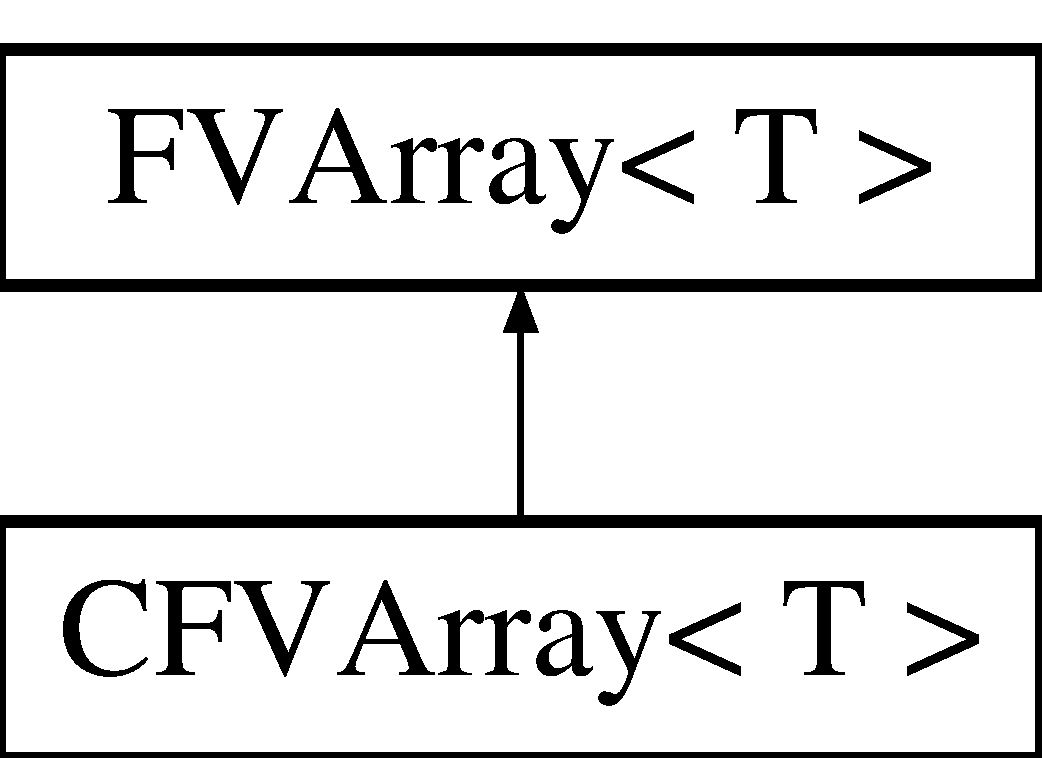
\includegraphics[height=2.000000cm]{d0/d1a/classFVL_1_1FVArray}
\end{center}
\end{figure}
\subsection*{Public Member Functions}
\begin{DoxyCompactItemize}
\item 
\hyperlink{classFVL_1_1FVArray_aa561520ffeba251ff13b97e6507e9356}{FVArray} (const unsigned int size)
\begin{DoxyCompactList}\small\item\em Constructor to create an array with a given size. \item\end{DoxyCompactList}\item 
\hyperlink{classFVL_1_1FVArray_a47404d96b43a8511ebbc2ddd4fbd8752}{FVArray} (const \hyperlink{classFVL_1_1FVArray}{FVArray}$<$ T $>$ \&copy)
\begin{DoxyCompactList}\small\item\em Constructor to create an array by copying an already existing array. \item\end{DoxyCompactList}\item 
\hyperlink{classFVL_1_1FVArray_a0158998b288980980fbd934dd00ba55b}{$\sim$FVArray} ()
\begin{DoxyCompactList}\small\item\em Default destructor. \item\end{DoxyCompactList}\item 
T \& \hyperlink{classFVL_1_1FVArray_a2d4b36a43041d6505f82836a6aeccd52}{operator\mbox{[}$\,$\mbox{]}} (int index)
\begin{DoxyCompactList}\small\item\em Array accessor as lvalue. \item\end{DoxyCompactList}\item 
const T \& \hyperlink{classFVL_1_1FVArray_a56e773dcafc33b12d2b27d2c7a174f3a}{operator\mbox{[}$\,$\mbox{]}} (int index) const 
\begin{DoxyCompactList}\small\item\em Array accessor as rvalue. \item\end{DoxyCompactList}\item 
const \hyperlink{classFVL_1_1FVArray}{FVArray}$<$ T $>$ \& \hyperlink{classFVL_1_1FVArray_a800962abf6eb71a43d99c156793fd5c5}{operator=} (const \hyperlink{classFVL_1_1FVArray}{FVArray}$<$ T $>$ \&copy)
\begin{DoxyCompactList}\small\item\em Assignment operator. \item\end{DoxyCompactList}\item 
T $\ast$ \hyperlink{classFVL_1_1FVArray_ad57caa1a97910998e7b9453ccbb3831c}{getArray} ()
\begin{DoxyCompactList}\small\item\em Gives direct access to array memory. \item\end{DoxyCompactList}\item 
unsigned int \hyperlink{classFVL_1_1FVArray_a90ca964ebcc1b02bbcde225edd49e812}{size} () const 
\begin{DoxyCompactList}\small\item\em Gives size of the array (number of elements). \item\end{DoxyCompactList}\end{DoxyCompactItemize}
\subsection*{Data Fields}
\begin{DoxyCompactItemize}
\item 
unsigned int \hyperlink{classFVL_1_1FVArray_a34a728cbcdbff333ec99c822697e3679}{arr\_\-size}
\begin{DoxyCompactList}\small\item\em number of elems allocated \item\end{DoxyCompactList}\item 
T $\ast$ \hyperlink{classFVL_1_1FVArray_a146e9e7358f9c0ad7b78c73519623f6c}{arr}
\begin{DoxyCompactList}\small\item\em Ptr to array memory. \item\end{DoxyCompactList}\end{DoxyCompactItemize}


\subsection{Detailed Description}
\subsubsection*{template$<$class T$>$ class FVL::FVArray$<$ T $>$}

Generic array template class. 

\subsection{Constructor \& Destructor Documentation}
\hypertarget{classFVL_1_1FVArray_aa561520ffeba251ff13b97e6507e9356}{
\index{FVL::FVArray@{FVL::FVArray}!FVArray@{FVArray}}
\index{FVArray@{FVArray}!FVL::FVArray@{FVL::FVArray}}
\subsubsection[{FVArray}]{\setlength{\rightskip}{0pt plus 5cm}{\bf FVArray} (
\begin{DoxyParamCaption}
\item[{const unsigned int}]{ size}
\end{DoxyParamCaption}
)}}
\label{d0/d1a/classFVL_1_1FVArray_aa561520ffeba251ff13b97e6507e9356}


Constructor to create an array with a given size. 


\begin{DoxyParams}{Parameters}
\item[{\em size}]Number of elements to allocate for the array \end{DoxyParams}
\hypertarget{classFVL_1_1FVArray_a47404d96b43a8511ebbc2ddd4fbd8752}{
\index{FVL::FVArray@{FVL::FVArray}!FVArray@{FVArray}}
\index{FVArray@{FVArray}!FVL::FVArray@{FVL::FVArray}}
\subsubsection[{FVArray}]{\setlength{\rightskip}{0pt plus 5cm}{\bf FVArray} (
\begin{DoxyParamCaption}
\item[{const {\bf FVArray}$<$ T $>$ \&}]{ copy}
\end{DoxyParamCaption}
)}}
\label{d0/d1a/classFVL_1_1FVArray_a47404d96b43a8511ebbc2ddd4fbd8752}


Constructor to create an array by copying an already existing array. 


\begin{DoxyParams}{Parameters}
\item[{\em copy}]Array to copy \end{DoxyParams}
\hypertarget{classFVL_1_1FVArray_a0158998b288980980fbd934dd00ba55b}{
\index{FVL::FVArray@{FVL::FVArray}!$\sim$FVArray@{$\sim$FVArray}}
\index{$\sim$FVArray@{$\sim$FVArray}!FVL::FVArray@{FVL::FVArray}}
\subsubsection[{$\sim$FVArray}]{\setlength{\rightskip}{0pt plus 5cm}$\sim${\bf FVArray} (
\begin{DoxyParamCaption}
{}
\end{DoxyParamCaption}
)}}
\label{d0/d1a/classFVL_1_1FVArray_a0158998b288980980fbd934dd00ba55b}


Default destructor. 

Releases all memory allocated for this array 

\subsection{Member Function Documentation}
\hypertarget{classFVL_1_1FVArray_ad57caa1a97910998e7b9453ccbb3831c}{
\index{FVL::FVArray@{FVL::FVArray}!getArray@{getArray}}
\index{getArray@{getArray}!FVL::FVArray@{FVL::FVArray}}
\subsubsection[{getArray}]{\setlength{\rightskip}{0pt plus 5cm}T$\ast$ getArray (
\begin{DoxyParamCaption}
{}
\end{DoxyParamCaption}
)}}
\label{d0/d1a/classFVL_1_1FVArray_ad57caa1a97910998e7b9453ccbb3831c}


Gives direct access to array memory. 

\begin{DoxyReturn}{Returns}
Pointer to memory where array is allocated 
\end{DoxyReturn}
\hypertarget{classFVL_1_1FVArray_a800962abf6eb71a43d99c156793fd5c5}{
\index{FVL::FVArray@{FVL::FVArray}!operator=@{operator=}}
\index{operator=@{operator=}!FVL::FVArray@{FVL::FVArray}}
\subsubsection[{operator=}]{\setlength{\rightskip}{0pt plus 5cm}const {\bf FVArray}$<$T$>$\& {\bf operator}= (
\begin{DoxyParamCaption}
\item[{const {\bf FVArray}$<$ T $>$ \&}]{ copy}
\end{DoxyParamCaption}
)}}
\label{d0/d1a/classFVL_1_1FVArray_a800962abf6eb71a43d99c156793fd5c5}


Assignment operator. 

Reallocate this array and create a hard copy of the parameter \hyperlink{classFVL_1_1FVArray_aa561520ffeba251ff13b97e6507e9356}{FVArray}


\begin{DoxyParams}{Parameters}
\item[{\em copy}]\hyperlink{classFVL_1_1FVArray_aa561520ffeba251ff13b97e6507e9356}{FVArray} to copy \end{DoxyParams}
\begin{DoxyReturn}{Returns}
Reference to the newly created \hyperlink{classFVL_1_1FVArray_aa561520ffeba251ff13b97e6507e9356}{FVArray} 
\end{DoxyReturn}
\hypertarget{classFVL_1_1FVArray_a56e773dcafc33b12d2b27d2c7a174f3a}{
\index{FVL::FVArray@{FVL::FVArray}!operator\mbox{[}\mbox{]}@{operator[]}}
\index{operator\mbox{[}\mbox{]}@{operator[]}!FVL::FVArray@{FVL::FVArray}}
\subsubsection[{operator[]}]{\setlength{\rightskip}{0pt plus 5cm}const T\& {\bf operator}\mbox{[}$\,$\mbox{]} (
\begin{DoxyParamCaption}
\item[{int}]{ index}
\end{DoxyParamCaption}
) const}}
\label{d0/d1a/classFVL_1_1FVArray_a56e773dcafc33b12d2b27d2c7a174f3a}


Array accessor as rvalue. 

Provides read-\/only acess to a given element


\begin{DoxyParams}{Parameters}
\item[{\em index}]position of the array to access \end{DoxyParams}
\begin{DoxyReturn}{Returns}
Constant reference to selected position of the array 
\end{DoxyReturn}
\hypertarget{classFVL_1_1FVArray_a2d4b36a43041d6505f82836a6aeccd52}{
\index{FVL::FVArray@{FVL::FVArray}!operator\mbox{[}\mbox{]}@{operator[]}}
\index{operator\mbox{[}\mbox{]}@{operator[]}!FVL::FVArray@{FVL::FVArray}}
\subsubsection[{operator[]}]{\setlength{\rightskip}{0pt plus 5cm}T\& {\bf operator}\mbox{[}$\,$\mbox{]} (
\begin{DoxyParamCaption}
\item[{int}]{ index}
\end{DoxyParamCaption}
)}}
\label{d0/d1a/classFVL_1_1FVArray_a2d4b36a43041d6505f82836a6aeccd52}


Array accessor as lvalue. 


\begin{DoxyParams}{Parameters}
\item[{\em index}]position of the array to acess \end{DoxyParams}
\begin{DoxyReturn}{Returns}
Modifiable reference to selected position of the array 
\end{DoxyReturn}
\hypertarget{classFVL_1_1FVArray_a90ca964ebcc1b02bbcde225edd49e812}{
\index{FVL::FVArray@{FVL::FVArray}!size@{size}}
\index{size@{size}!FVL::FVArray@{FVL::FVArray}}
\subsubsection[{size}]{\setlength{\rightskip}{0pt plus 5cm}unsigned int size (
\begin{DoxyParamCaption}
{}
\end{DoxyParamCaption}
) const}}
\label{d0/d1a/classFVL_1_1FVArray_a90ca964ebcc1b02bbcde225edd49e812}


Gives size of the array (number of elements). 

\begin{DoxyReturn}{Returns}
total number of elements allocated 
\end{DoxyReturn}


\subsection{Field Documentation}
\hypertarget{classFVL_1_1FVArray_a146e9e7358f9c0ad7b78c73519623f6c}{
\index{FVL::FVArray@{FVL::FVArray}!arr@{arr}}
\index{arr@{arr}!FVL::FVArray@{FVL::FVArray}}
\subsubsection[{arr}]{\setlength{\rightskip}{0pt plus 5cm}T$\ast$ {\bf arr}}}
\label{d0/d1a/classFVL_1_1FVArray_a146e9e7358f9c0ad7b78c73519623f6c}


Ptr to array memory. 

\hypertarget{classFVL_1_1FVArray_a34a728cbcdbff333ec99c822697e3679}{
\index{FVL::FVArray@{FVL::FVArray}!arr\_\-size@{arr\_\-size}}
\index{arr\_\-size@{arr\_\-size}!FVL::FVArray@{FVL::FVArray}}
\subsubsection[{arr\_\-size}]{\setlength{\rightskip}{0pt plus 5cm}unsigned int {\bf arr\_\-size}}}
\label{d0/d1a/classFVL_1_1FVArray_a34a728cbcdbff333ec99c822697e3679}


number of elems allocated 



The documentation for this class was generated from the following file:\begin{DoxyCompactItemize}
\item 
include/FVL/\hyperlink{FVArray_8h}{FVArray.h}\end{DoxyCompactItemize}

\hypertarget{classFVCell1D}{
\section{FVCell1D Class Reference}
\label{dc/df2/classFVCell1D}\index{FVCell1D@{FVCell1D}}
}


{\ttfamily \#include $<$FVCell1D.h$>$}

\subsection*{Public Member Functions}
\begin{DoxyCompactItemize}
\item 
\hyperlink{classFVCell1D_a6383b88a96eb8a8ca85c8e9f5ba17748}{FVCell1D} ()
\item 
\hyperlink{classFVCell1D_a0ddd36288947988899310777d6f79e21}{$\sim$FVCell1D} ()
\item 
\hyperlink{classFVVertex1D}{FVVertex1D} $\ast$ \hyperlink{classFVCell1D_ad4fad0e0941476b665cf09b20c6f3d93}{beginVertex} ()
\item 
\hyperlink{classFVVertex1D}{FVVertex1D} $\ast$ \hyperlink{classFVCell1D_ab7a9cc3e82cb21cd210ff298bb9b4794}{nextVertex} ()
\item 
void \hyperlink{classFVCell1D_a0a47b3287cfccb79cba1552f3ad1e7b9}{setCode2Vertex} (size\_\-t val=0)
\end{DoxyCompactItemize}
\subsection*{Data Fields}
\begin{DoxyCompactItemize}
\item 
\hyperlink{classFVPoint1D}{FVPoint1D}$<$ double $>$ \hyperlink{classFVCell1D_aaff9d346ae9979beebf810a5b6ade9ad}{centroid}
\item 
double \hyperlink{classFVCell1D_a928b11f5716331f0b89abe7d8d4124b4}{length}
\item 
size\_\-t \hyperlink{classFVCell1D_a1ec973463c76e6d9e91160720959ad68}{label}
\item 
size\_\-t \hyperlink{classFVCell1D_acf258c3b3328a96e3ee1e3b875b7874f}{code}
\item 
size\_\-t \hyperlink{classFVCell1D_a0a063e99fbc85e837d93dfbcda6f5252}{nb\_\-vertex}
\item 
\hyperlink{classFVVertex1D}{FVVertex1D} $\ast$ \hyperlink{classFVCell1D_aeb8a64ff3e2005419385cb290aeea4da}{firstVertex}
\item 
\hyperlink{classFVVertex1D}{FVVertex1D} $\ast$ \hyperlink{classFVCell1D_afae31f3f40827a0997d66b07c4a040c2}{secondVertex}
\item 
\hyperlink{classFVPoint1D}{FVPoint1D}$<$ double $>$ \hyperlink{classFVCell1D_ab9bb84e59374f4fbdeb16ba2e4c22fed}{first\_\-normal}
\item 
\hyperlink{classFVPoint1D}{FVPoint1D}$<$ double $>$ \hyperlink{classFVCell1D_afcc978d58cef2439dc0587b60e3fb727}{second\_\-normal}
\end{DoxyCompactItemize}


\subsection{Constructor \& Destructor Documentation}
\hypertarget{classFVCell1D_a6383b88a96eb8a8ca85c8e9f5ba17748}{
\index{FVCell1D@{FVCell1D}!FVCell1D@{FVCell1D}}
\index{FVCell1D@{FVCell1D}!FVCell1D@{FVCell1D}}
\subsubsection[{FVCell1D}]{\setlength{\rightskip}{0pt plus 5cm}{\bf FVCell1D} (
\begin{DoxyParamCaption}
{}
\end{DoxyParamCaption}
)\hspace{0.3cm}{\ttfamily  \mbox{[}inline\mbox{]}}}}
\label{dc/df2/classFVCell1D_a6383b88a96eb8a8ca85c8e9f5ba17748}
\hypertarget{classFVCell1D_a0ddd36288947988899310777d6f79e21}{
\index{FVCell1D@{FVCell1D}!$\sim$FVCell1D@{$\sim$FVCell1D}}
\index{$\sim$FVCell1D@{$\sim$FVCell1D}!FVCell1D@{FVCell1D}}
\subsubsection[{$\sim$FVCell1D}]{\setlength{\rightskip}{0pt plus 5cm}$\sim${\bf FVCell1D} (
\begin{DoxyParamCaption}
{}
\end{DoxyParamCaption}
)\hspace{0.3cm}{\ttfamily  \mbox{[}inline\mbox{]}}}}
\label{dc/df2/classFVCell1D_a0ddd36288947988899310777d6f79e21}


\subsection{Member Function Documentation}
\hypertarget{classFVCell1D_ad4fad0e0941476b665cf09b20c6f3d93}{
\index{FVCell1D@{FVCell1D}!beginVertex@{beginVertex}}
\index{beginVertex@{beginVertex}!FVCell1D@{FVCell1D}}
\subsubsection[{beginVertex}]{\setlength{\rightskip}{0pt plus 5cm}{\bf FVVertex1D}$\ast$ beginVertex (
\begin{DoxyParamCaption}
{}
\end{DoxyParamCaption}
)\hspace{0.3cm}{\ttfamily  \mbox{[}inline\mbox{]}}}}
\label{dc/df2/classFVCell1D_ad4fad0e0941476b665cf09b20c6f3d93}
\hypertarget{classFVCell1D_ab7a9cc3e82cb21cd210ff298bb9b4794}{
\index{FVCell1D@{FVCell1D}!nextVertex@{nextVertex}}
\index{nextVertex@{nextVertex}!FVCell1D@{FVCell1D}}
\subsubsection[{nextVertex}]{\setlength{\rightskip}{0pt plus 5cm}{\bf FVVertex1D}$\ast$ nextVertex (
\begin{DoxyParamCaption}
{}
\end{DoxyParamCaption}
)\hspace{0.3cm}{\ttfamily  \mbox{[}inline\mbox{]}}}}
\label{dc/df2/classFVCell1D_ab7a9cc3e82cb21cd210ff298bb9b4794}
\hypertarget{classFVCell1D_a0a47b3287cfccb79cba1552f3ad1e7b9}{
\index{FVCell1D@{FVCell1D}!setCode2Vertex@{setCode2Vertex}}
\index{setCode2Vertex@{setCode2Vertex}!FVCell1D@{FVCell1D}}
\subsubsection[{setCode2Vertex}]{\setlength{\rightskip}{0pt plus 5cm}void setCode2Vertex (
\begin{DoxyParamCaption}
\item[{size\_\-t}]{ val = {\ttfamily 0}}
\end{DoxyParamCaption}
)\hspace{0.3cm}{\ttfamily  \mbox{[}inline\mbox{]}}}}
\label{dc/df2/classFVCell1D_a0a47b3287cfccb79cba1552f3ad1e7b9}


\subsection{Field Documentation}
\hypertarget{classFVCell1D_aaff9d346ae9979beebf810a5b6ade9ad}{
\index{FVCell1D@{FVCell1D}!centroid@{centroid}}
\index{centroid@{centroid}!FVCell1D@{FVCell1D}}
\subsubsection[{centroid}]{\setlength{\rightskip}{0pt plus 5cm}{\bf FVPoint1D}$<$double$>$ {\bf centroid}}}
\label{dc/df2/classFVCell1D_aaff9d346ae9979beebf810a5b6ade9ad}
\hypertarget{classFVCell1D_acf258c3b3328a96e3ee1e3b875b7874f}{
\index{FVCell1D@{FVCell1D}!code@{code}}
\index{code@{code}!FVCell1D@{FVCell1D}}
\subsubsection[{code}]{\setlength{\rightskip}{0pt plus 5cm}size\_\-t {\bf code}}}
\label{dc/df2/classFVCell1D_acf258c3b3328a96e3ee1e3b875b7874f}
\hypertarget{classFVCell1D_ab9bb84e59374f4fbdeb16ba2e4c22fed}{
\index{FVCell1D@{FVCell1D}!first\_\-normal@{first\_\-normal}}
\index{first\_\-normal@{first\_\-normal}!FVCell1D@{FVCell1D}}
\subsubsection[{first\_\-normal}]{\setlength{\rightskip}{0pt plus 5cm}{\bf FVPoint1D}$<$double$>$ {\bf first\_\-normal}}}
\label{dc/df2/classFVCell1D_ab9bb84e59374f4fbdeb16ba2e4c22fed}
\hypertarget{classFVCell1D_aeb8a64ff3e2005419385cb290aeea4da}{
\index{FVCell1D@{FVCell1D}!firstVertex@{firstVertex}}
\index{firstVertex@{firstVertex}!FVCell1D@{FVCell1D}}
\subsubsection[{firstVertex}]{\setlength{\rightskip}{0pt plus 5cm}{\bf FVVertex1D}$\ast$ {\bf firstVertex}}}
\label{dc/df2/classFVCell1D_aeb8a64ff3e2005419385cb290aeea4da}
\hypertarget{classFVCell1D_a1ec973463c76e6d9e91160720959ad68}{
\index{FVCell1D@{FVCell1D}!label@{label}}
\index{label@{label}!FVCell1D@{FVCell1D}}
\subsubsection[{label}]{\setlength{\rightskip}{0pt plus 5cm}size\_\-t {\bf label}}}
\label{dc/df2/classFVCell1D_a1ec973463c76e6d9e91160720959ad68}
\hypertarget{classFVCell1D_a928b11f5716331f0b89abe7d8d4124b4}{
\index{FVCell1D@{FVCell1D}!length@{length}}
\index{length@{length}!FVCell1D@{FVCell1D}}
\subsubsection[{length}]{\setlength{\rightskip}{0pt plus 5cm}double {\bf length}}}
\label{dc/df2/classFVCell1D_a928b11f5716331f0b89abe7d8d4124b4}
\hypertarget{classFVCell1D_a0a063e99fbc85e837d93dfbcda6f5252}{
\index{FVCell1D@{FVCell1D}!nb\_\-vertex@{nb\_\-vertex}}
\index{nb\_\-vertex@{nb\_\-vertex}!FVCell1D@{FVCell1D}}
\subsubsection[{nb\_\-vertex}]{\setlength{\rightskip}{0pt plus 5cm}size\_\-t {\bf nb\_\-vertex}}}
\label{dc/df2/classFVCell1D_a0a063e99fbc85e837d93dfbcda6f5252}
\hypertarget{classFVCell1D_afcc978d58cef2439dc0587b60e3fb727}{
\index{FVCell1D@{FVCell1D}!second\_\-normal@{second\_\-normal}}
\index{second\_\-normal@{second\_\-normal}!FVCell1D@{FVCell1D}}
\subsubsection[{second\_\-normal}]{\setlength{\rightskip}{0pt plus 5cm}{\bf FVPoint1D}$<$double$>$ {\bf second\_\-normal}}}
\label{dc/df2/classFVCell1D_afcc978d58cef2439dc0587b60e3fb727}
\hypertarget{classFVCell1D_afae31f3f40827a0997d66b07c4a040c2}{
\index{FVCell1D@{FVCell1D}!secondVertex@{secondVertex}}
\index{secondVertex@{secondVertex}!FVCell1D@{FVCell1D}}
\subsubsection[{secondVertex}]{\setlength{\rightskip}{0pt plus 5cm}{\bf FVVertex1D} $\ast$ {\bf secondVertex}}}
\label{dc/df2/classFVCell1D_afae31f3f40827a0997d66b07c4a040c2}


The documentation for this class was generated from the following file:\begin{DoxyCompactItemize}
\item 
include/\hyperlink{FVCell1D_8h}{FVCell1D.h}\end{DoxyCompactItemize}

\hypertarget{classFVCell2D}{
\section{FVCell2D Class Reference}
\label{da/da3/classFVCell2D}\index{FVCell2D@{FVCell2D}}
}


{\ttfamily \#include $<$FVCell2D.h$>$}

\subsection*{Public Member Functions}
\begin{DoxyCompactItemize}
\item 
\hyperlink{classFVCell2D_ae1be13799d8d42fcb7aebe7fe88bda3f}{FVCell2D} ()
\item 
\hyperlink{classFVCell2D_abed3be74677406373585410b9e523124}{$\sim$FVCell2D} ()
\item 
\hyperlink{classFVVertex2D}{FVVertex2D} $\ast$ \hyperlink{classFVCell2D_a67415ad3823d1cd8030deaa6c4123f45}{beginVertex} ()
\item 
\hyperlink{classFVVertex2D}{FVVertex2D} $\ast$ \hyperlink{classFVCell2D_a18cc99908c3657e8afe0e7b5feee5c23}{nextVertex} ()
\item 
\hyperlink{classFVEdge2D}{FVEdge2D} $\ast$ \hyperlink{classFVCell2D_a1ae842934bc9c9c5d246f70ff2413057}{beginEdge} ()
\item 
\hyperlink{classFVEdge2D}{FVEdge2D} $\ast$ \hyperlink{classFVCell2D_a3616f047ec627e0ccc4c30343e9b24ef}{nextEdge} ()
\item 
FVPoint2D$<$ double $>$ \hyperlink{classFVCell2D_ab303dcc1c05e3294ff6cb25dcf088fe2}{getCell2Edge} ()
\item 
void \hyperlink{classFVCell2D_a9e25d24a18a62921eff34d38f8b1b896}{setCode2Edge} (size\_\-t val=0)
\item 
void \hyperlink{classFVCell2D_a0a47b3287cfccb79cba1552f3ad1e7b9}{setCode2Vertex} (size\_\-t val=0)
\end{DoxyCompactItemize}
\subsection*{Data Fields}
\begin{DoxyCompactItemize}
\item 
FVPoint2D$<$ double $>$ \hyperlink{classFVCell2D_ab3ed78ad91cf05def39147f46817c454}{centroid}
\item 
size\_\-t \hyperlink{classFVCell2D_a1ec973463c76e6d9e91160720959ad68}{label}
\item 
size\_\-t \hyperlink{classFVCell2D_acf258c3b3328a96e3ee1e3b875b7874f}{code}
\item 
size\_\-t \hyperlink{classFVCell2D_a0a063e99fbc85e837d93dfbcda6f5252}{nb\_\-vertex}
\item 
size\_\-t \hyperlink{classFVCell2D_a71d1c26cc375a03060b9eb8453a3680a}{nb\_\-edge}
\item 
size\_\-t \hyperlink{classFVCell2D_a6320f7771a5dd32537e636a23fbf7e7c}{pos\_\-e}
\item 
size\_\-t \hyperlink{classFVCell2D_a9edf0688f0159bed5d3a6828f63146fd}{pos\_\-v}
\item 
double \hyperlink{classFVCell2D_a079d8fd569c3406fb63e0511eb0338c0}{perimeter}
\item 
double \hyperlink{classFVCell2D_ae517bffd82b9428b4f1d9500ea01c04f}{area}
\item 
\hyperlink{classFVVertex2D}{FVVertex2D} $\ast$ \hyperlink{classFVCell2D_a43af246790b321630c5b93c98d944c4e}{vertex} \mbox{[}NB\_\-VERTEX\_\-PER\_\-CELL\_\-2D\mbox{]}
\item 
\hyperlink{classFVEdge2D}{FVEdge2D} $\ast$ \hyperlink{classFVCell2D_aaef61084c7d087b06124b4e122b26eba}{edge} \mbox{[}NB\_\-EDGE\_\-PER\_\-CELL\_\-2D\mbox{]}
\item 
FVPoint2D$<$ double $>$ \hyperlink{classFVCell2D_a99bffb94997ba2dc39e4184c17166cce}{cell2edge} \mbox{[}NB\_\-EDGE\_\-PER\_\-CELL\_\-2D\mbox{]}
\end{DoxyCompactItemize}


\subsection{Constructor \& Destructor Documentation}
\hypertarget{classFVCell2D_ae1be13799d8d42fcb7aebe7fe88bda3f}{
\index{FVCell2D@{FVCell2D}!FVCell2D@{FVCell2D}}
\index{FVCell2D@{FVCell2D}!FVCell2D@{FVCell2D}}
\subsubsection[{FVCell2D}]{\setlength{\rightskip}{0pt plus 5cm}{\bf FVCell2D} (
\begin{DoxyParamCaption}
{}
\end{DoxyParamCaption}
)\hspace{0.3cm}{\ttfamily  \mbox{[}inline\mbox{]}}}}
\label{da/da3/classFVCell2D_ae1be13799d8d42fcb7aebe7fe88bda3f}
\hypertarget{classFVCell2D_abed3be74677406373585410b9e523124}{
\index{FVCell2D@{FVCell2D}!$\sim$FVCell2D@{$\sim$FVCell2D}}
\index{$\sim$FVCell2D@{$\sim$FVCell2D}!FVCell2D@{FVCell2D}}
\subsubsection[{$\sim$FVCell2D}]{\setlength{\rightskip}{0pt plus 5cm}$\sim${\bf FVCell2D} (
\begin{DoxyParamCaption}
{}
\end{DoxyParamCaption}
)\hspace{0.3cm}{\ttfamily  \mbox{[}inline\mbox{]}}}}
\label{da/da3/classFVCell2D_abed3be74677406373585410b9e523124}


\subsection{Member Function Documentation}
\hypertarget{classFVCell2D_a1ae842934bc9c9c5d246f70ff2413057}{
\index{FVCell2D@{FVCell2D}!beginEdge@{beginEdge}}
\index{beginEdge@{beginEdge}!FVCell2D@{FVCell2D}}
\subsubsection[{beginEdge}]{\setlength{\rightskip}{0pt plus 5cm}{\bf FVEdge2D}$\ast$ beginEdge (
\begin{DoxyParamCaption}
{}
\end{DoxyParamCaption}
)\hspace{0.3cm}{\ttfamily  \mbox{[}inline\mbox{]}}}}
\label{da/da3/classFVCell2D_a1ae842934bc9c9c5d246f70ff2413057}
\hypertarget{classFVCell2D_a67415ad3823d1cd8030deaa6c4123f45}{
\index{FVCell2D@{FVCell2D}!beginVertex@{beginVertex}}
\index{beginVertex@{beginVertex}!FVCell2D@{FVCell2D}}
\subsubsection[{beginVertex}]{\setlength{\rightskip}{0pt plus 5cm}{\bf FVVertex2D}$\ast$ beginVertex (
\begin{DoxyParamCaption}
{}
\end{DoxyParamCaption}
)\hspace{0.3cm}{\ttfamily  \mbox{[}inline\mbox{]}}}}
\label{da/da3/classFVCell2D_a67415ad3823d1cd8030deaa6c4123f45}
\hypertarget{classFVCell2D_ab303dcc1c05e3294ff6cb25dcf088fe2}{
\index{FVCell2D@{FVCell2D}!getCell2Edge@{getCell2Edge}}
\index{getCell2Edge@{getCell2Edge}!FVCell2D@{FVCell2D}}
\subsubsection[{getCell2Edge}]{\setlength{\rightskip}{0pt plus 5cm}FVPoint2D$<$double$>$ getCell2Edge (
\begin{DoxyParamCaption}
{}
\end{DoxyParamCaption}
)\hspace{0.3cm}{\ttfamily  \mbox{[}inline\mbox{]}}}}
\label{da/da3/classFVCell2D_ab303dcc1c05e3294ff6cb25dcf088fe2}
\hypertarget{classFVCell2D_a3616f047ec627e0ccc4c30343e9b24ef}{
\index{FVCell2D@{FVCell2D}!nextEdge@{nextEdge}}
\index{nextEdge@{nextEdge}!FVCell2D@{FVCell2D}}
\subsubsection[{nextEdge}]{\setlength{\rightskip}{0pt plus 5cm}{\bf FVEdge2D}$\ast$ nextEdge (
\begin{DoxyParamCaption}
{}
\end{DoxyParamCaption}
)\hspace{0.3cm}{\ttfamily  \mbox{[}inline\mbox{]}}}}
\label{da/da3/classFVCell2D_a3616f047ec627e0ccc4c30343e9b24ef}
\hypertarget{classFVCell2D_a18cc99908c3657e8afe0e7b5feee5c23}{
\index{FVCell2D@{FVCell2D}!nextVertex@{nextVertex}}
\index{nextVertex@{nextVertex}!FVCell2D@{FVCell2D}}
\subsubsection[{nextVertex}]{\setlength{\rightskip}{0pt plus 5cm}{\bf FVVertex2D}$\ast$ nextVertex (
\begin{DoxyParamCaption}
{}
\end{DoxyParamCaption}
)\hspace{0.3cm}{\ttfamily  \mbox{[}inline\mbox{]}}}}
\label{da/da3/classFVCell2D_a18cc99908c3657e8afe0e7b5feee5c23}
\hypertarget{classFVCell2D_a9e25d24a18a62921eff34d38f8b1b896}{
\index{FVCell2D@{FVCell2D}!setCode2Edge@{setCode2Edge}}
\index{setCode2Edge@{setCode2Edge}!FVCell2D@{FVCell2D}}
\subsubsection[{setCode2Edge}]{\setlength{\rightskip}{0pt plus 5cm}void setCode2Edge (
\begin{DoxyParamCaption}
\item[{size\_\-t}]{ val = {\ttfamily 0}}
\end{DoxyParamCaption}
)\hspace{0.3cm}{\ttfamily  \mbox{[}inline\mbox{]}}}}
\label{da/da3/classFVCell2D_a9e25d24a18a62921eff34d38f8b1b896}
\hypertarget{classFVCell2D_a0a47b3287cfccb79cba1552f3ad1e7b9}{
\index{FVCell2D@{FVCell2D}!setCode2Vertex@{setCode2Vertex}}
\index{setCode2Vertex@{setCode2Vertex}!FVCell2D@{FVCell2D}}
\subsubsection[{setCode2Vertex}]{\setlength{\rightskip}{0pt plus 5cm}void setCode2Vertex (
\begin{DoxyParamCaption}
\item[{size\_\-t}]{ val = {\ttfamily 0}}
\end{DoxyParamCaption}
)\hspace{0.3cm}{\ttfamily  \mbox{[}inline\mbox{]}}}}
\label{da/da3/classFVCell2D_a0a47b3287cfccb79cba1552f3ad1e7b9}


\subsection{Field Documentation}
\hypertarget{classFVCell2D_ae517bffd82b9428b4f1d9500ea01c04f}{
\index{FVCell2D@{FVCell2D}!area@{area}}
\index{area@{area}!FVCell2D@{FVCell2D}}
\subsubsection[{area}]{\setlength{\rightskip}{0pt plus 5cm}double {\bf area}}}
\label{da/da3/classFVCell2D_ae517bffd82b9428b4f1d9500ea01c04f}
\hypertarget{classFVCell2D_a99bffb94997ba2dc39e4184c17166cce}{
\index{FVCell2D@{FVCell2D}!cell2edge@{cell2edge}}
\index{cell2edge@{cell2edge}!FVCell2D@{FVCell2D}}
\subsubsection[{cell2edge}]{\setlength{\rightskip}{0pt plus 5cm}FVPoint2D$<$double$>$ {\bf cell2edge}\mbox{[}NB\_\-EDGE\_\-PER\_\-CELL\_\-2D\mbox{]}}}
\label{da/da3/classFVCell2D_a99bffb94997ba2dc39e4184c17166cce}
\hypertarget{classFVCell2D_ab3ed78ad91cf05def39147f46817c454}{
\index{FVCell2D@{FVCell2D}!centroid@{centroid}}
\index{centroid@{centroid}!FVCell2D@{FVCell2D}}
\subsubsection[{centroid}]{\setlength{\rightskip}{0pt plus 5cm}FVPoint2D$<$double$>$ {\bf centroid}}}
\label{da/da3/classFVCell2D_ab3ed78ad91cf05def39147f46817c454}
\hypertarget{classFVCell2D_acf258c3b3328a96e3ee1e3b875b7874f}{
\index{FVCell2D@{FVCell2D}!code@{code}}
\index{code@{code}!FVCell2D@{FVCell2D}}
\subsubsection[{code}]{\setlength{\rightskip}{0pt plus 5cm}size\_\-t {\bf code}}}
\label{da/da3/classFVCell2D_acf258c3b3328a96e3ee1e3b875b7874f}
\hypertarget{classFVCell2D_aaef61084c7d087b06124b4e122b26eba}{
\index{FVCell2D@{FVCell2D}!edge@{edge}}
\index{edge@{edge}!FVCell2D@{FVCell2D}}
\subsubsection[{edge}]{\setlength{\rightskip}{0pt plus 5cm}{\bf FVEdge2D}$\ast$ {\bf edge}\mbox{[}NB\_\-EDGE\_\-PER\_\-CELL\_\-2D\mbox{]}}}
\label{da/da3/classFVCell2D_aaef61084c7d087b06124b4e122b26eba}
\hypertarget{classFVCell2D_a1ec973463c76e6d9e91160720959ad68}{
\index{FVCell2D@{FVCell2D}!label@{label}}
\index{label@{label}!FVCell2D@{FVCell2D}}
\subsubsection[{label}]{\setlength{\rightskip}{0pt plus 5cm}size\_\-t {\bf label}}}
\label{da/da3/classFVCell2D_a1ec973463c76e6d9e91160720959ad68}
\hypertarget{classFVCell2D_a71d1c26cc375a03060b9eb8453a3680a}{
\index{FVCell2D@{FVCell2D}!nb\_\-edge@{nb\_\-edge}}
\index{nb\_\-edge@{nb\_\-edge}!FVCell2D@{FVCell2D}}
\subsubsection[{nb\_\-edge}]{\setlength{\rightskip}{0pt plus 5cm}size\_\-t {\bf nb\_\-edge}}}
\label{da/da3/classFVCell2D_a71d1c26cc375a03060b9eb8453a3680a}
\hypertarget{classFVCell2D_a0a063e99fbc85e837d93dfbcda6f5252}{
\index{FVCell2D@{FVCell2D}!nb\_\-vertex@{nb\_\-vertex}}
\index{nb\_\-vertex@{nb\_\-vertex}!FVCell2D@{FVCell2D}}
\subsubsection[{nb\_\-vertex}]{\setlength{\rightskip}{0pt plus 5cm}size\_\-t {\bf nb\_\-vertex}}}
\label{da/da3/classFVCell2D_a0a063e99fbc85e837d93dfbcda6f5252}
\hypertarget{classFVCell2D_a079d8fd569c3406fb63e0511eb0338c0}{
\index{FVCell2D@{FVCell2D}!perimeter@{perimeter}}
\index{perimeter@{perimeter}!FVCell2D@{FVCell2D}}
\subsubsection[{perimeter}]{\setlength{\rightskip}{0pt plus 5cm}double {\bf perimeter}}}
\label{da/da3/classFVCell2D_a079d8fd569c3406fb63e0511eb0338c0}
\hypertarget{classFVCell2D_a6320f7771a5dd32537e636a23fbf7e7c}{
\index{FVCell2D@{FVCell2D}!pos\_\-e@{pos\_\-e}}
\index{pos\_\-e@{pos\_\-e}!FVCell2D@{FVCell2D}}
\subsubsection[{pos\_\-e}]{\setlength{\rightskip}{0pt plus 5cm}size\_\-t {\bf pos\_\-e}}}
\label{da/da3/classFVCell2D_a6320f7771a5dd32537e636a23fbf7e7c}
\hypertarget{classFVCell2D_a9edf0688f0159bed5d3a6828f63146fd}{
\index{FVCell2D@{FVCell2D}!pos\_\-v@{pos\_\-v}}
\index{pos\_\-v@{pos\_\-v}!FVCell2D@{FVCell2D}}
\subsubsection[{pos\_\-v}]{\setlength{\rightskip}{0pt plus 5cm}size\_\-t {\bf pos\_\-v}}}
\label{da/da3/classFVCell2D_a9edf0688f0159bed5d3a6828f63146fd}
\hypertarget{classFVCell2D_a43af246790b321630c5b93c98d944c4e}{
\index{FVCell2D@{FVCell2D}!vertex@{vertex}}
\index{vertex@{vertex}!FVCell2D@{FVCell2D}}
\subsubsection[{vertex}]{\setlength{\rightskip}{0pt plus 5cm}{\bf FVVertex2D}$\ast$ {\bf vertex}\mbox{[}NB\_\-VERTEX\_\-PER\_\-CELL\_\-2D\mbox{]}}}
\label{da/da3/classFVCell2D_a43af246790b321630c5b93c98d944c4e}


The documentation for this class was generated from the following file:\begin{DoxyCompactItemize}
\item 
include/\hyperlink{FVCell2D_8h}{FVCell2D.h}\end{DoxyCompactItemize}

\hypertarget{classFVCell3D}{
\section{FVCell3D Class Reference}
\label{d0/ded/classFVCell3D}\index{FVCell3D@{FVCell3D}}
}


{\ttfamily \#include $<$FVCell3D.h$>$}

\subsection*{Public Member Functions}
\begin{DoxyCompactItemize}
\item 
\hyperlink{classFVCell3D_a49bd227b79650dd9cef19953d95b7cef}{FVCell3D} ()
\item 
\hyperlink{classFVCell3D_a889aa6d5cf332a937956788ce218389a}{$\sim$FVCell3D} ()
\item 
\hyperlink{classFVVertex3D}{FVVertex3D} $\ast$ \hyperlink{classFVCell3D_a00e03dd7e67cf78d0d00487e52394451}{beginVertex} ()
\item 
\hyperlink{classFVVertex3D}{FVVertex3D} $\ast$ \hyperlink{classFVCell3D_a936762a7544b61fc2a7bf156a3394d28}{nextVertex} ()
\item 
\hyperlink{classFVFace3D}{FVFace3D} $\ast$ \hyperlink{classFVCell3D_aa21193e45097be75beb98132a1586e58}{beginFace} ()
\item 
\hyperlink{classFVFace3D}{FVFace3D} $\ast$ \hyperlink{classFVCell3D_aa3011d7de736306ee0ab315acfcb73a7}{nextFace} ()
\item 
\hyperlink{classFVPoint3D}{FVPoint3D}$<$ double $>$ \hyperlink{classFVCell3D_afbdbd782a9de358a91b0875abb0b5220}{getCell2Face} ()
\item 
void \hyperlink{classFVCell3D_acbc323a04994b55b242f1023e6a29d1c}{setCode2Face} (size\_\-t val=0)
\item 
void \hyperlink{classFVCell3D_a9e25d24a18a62921eff34d38f8b1b896}{setCode2Edge} (size\_\-t val=0)
\item 
void \hyperlink{classFVCell3D_a0a47b3287cfccb79cba1552f3ad1e7b9}{setCode2Vertex} (size\_\-t val=0)
\end{DoxyCompactItemize}
\subsection*{Data Fields}
\begin{DoxyCompactItemize}
\item 
\hyperlink{classFVPoint3D}{FVPoint3D}$<$ double $>$ \hyperlink{classFVCell3D_af0e77c00d990c1a712cf032be1bb8f0f}{centroid}
\item 
size\_\-t \hyperlink{classFVCell3D_a1ec973463c76e6d9e91160720959ad68}{label}
\item 
size\_\-t \hyperlink{classFVCell3D_acf258c3b3328a96e3ee1e3b875b7874f}{code}
\item 
size\_\-t \hyperlink{classFVCell3D_a0a063e99fbc85e837d93dfbcda6f5252}{nb\_\-vertex}
\item 
size\_\-t \hyperlink{classFVCell3D_acafc91cfd098750db0bcbe840dbb283c}{nb\_\-face}
\item 
size\_\-t \hyperlink{classFVCell3D_a22e92dae91397209d0da1e056358fbd7}{pos\_\-f}
\item 
size\_\-t \hyperlink{classFVCell3D_a9edf0688f0159bed5d3a6828f63146fd}{pos\_\-v}
\item 
double \hyperlink{classFVCell3D_aec4a2e345c6aacee9bb86c610f0bfab6}{surface}
\item 
double \hyperlink{classFVCell3D_a8eb3ef4958b442309868039dbab6f0bf}{volume}
\item 
\hyperlink{classFVVertex3D}{FVVertex3D} $\ast$ \hyperlink{classFVCell3D_a7fe38788ed0792b47203a4fb432f523a}{vertex} \mbox{[}NB\_\-VERTEX\_\-PER\_\-CELL\_\-3D\mbox{]}
\item 
\hyperlink{classFVFace3D}{FVFace3D} $\ast$ \hyperlink{classFVCell3D_a1e22889f938f60a77af81fe2dd8423f9}{face} \mbox{[}NB\_\-FACE\_\-PER\_\-CELL\_\-3D\mbox{]}
\item 
\hyperlink{classFVPoint3D}{FVPoint3D}$<$ double $>$ \hyperlink{classFVCell3D_a13f89e3dcdbe5547a6ef0b92f3bb4583}{cell2face} \mbox{[}NB\_\-FACE\_\-PER\_\-CELL\_\-3D\mbox{]}
\end{DoxyCompactItemize}


\subsection{Constructor \& Destructor Documentation}
\hypertarget{classFVCell3D_a49bd227b79650dd9cef19953d95b7cef}{
\index{FVCell3D@{FVCell3D}!FVCell3D@{FVCell3D}}
\index{FVCell3D@{FVCell3D}!FVCell3D@{FVCell3D}}
\subsubsection[{FVCell3D}]{\setlength{\rightskip}{0pt plus 5cm}{\bf FVCell3D} (
\begin{DoxyParamCaption}
{}
\end{DoxyParamCaption}
)\hspace{0.3cm}{\ttfamily  \mbox{[}inline\mbox{]}}}}
\label{d0/ded/classFVCell3D_a49bd227b79650dd9cef19953d95b7cef}
\hypertarget{classFVCell3D_a889aa6d5cf332a937956788ce218389a}{
\index{FVCell3D@{FVCell3D}!$\sim$FVCell3D@{$\sim$FVCell3D}}
\index{$\sim$FVCell3D@{$\sim$FVCell3D}!FVCell3D@{FVCell3D}}
\subsubsection[{$\sim$FVCell3D}]{\setlength{\rightskip}{0pt plus 5cm}$\sim${\bf FVCell3D} (
\begin{DoxyParamCaption}
{}
\end{DoxyParamCaption}
)\hspace{0.3cm}{\ttfamily  \mbox{[}inline\mbox{]}}}}
\label{d0/ded/classFVCell3D_a889aa6d5cf332a937956788ce218389a}


\subsection{Member Function Documentation}
\hypertarget{classFVCell3D_aa21193e45097be75beb98132a1586e58}{
\index{FVCell3D@{FVCell3D}!beginFace@{beginFace}}
\index{beginFace@{beginFace}!FVCell3D@{FVCell3D}}
\subsubsection[{beginFace}]{\setlength{\rightskip}{0pt plus 5cm}{\bf FVFace3D}$\ast$ beginFace (
\begin{DoxyParamCaption}
{}
\end{DoxyParamCaption}
)\hspace{0.3cm}{\ttfamily  \mbox{[}inline\mbox{]}}}}
\label{d0/ded/classFVCell3D_aa21193e45097be75beb98132a1586e58}
\hypertarget{classFVCell3D_a00e03dd7e67cf78d0d00487e52394451}{
\index{FVCell3D@{FVCell3D}!beginVertex@{beginVertex}}
\index{beginVertex@{beginVertex}!FVCell3D@{FVCell3D}}
\subsubsection[{beginVertex}]{\setlength{\rightskip}{0pt plus 5cm}{\bf FVVertex3D}$\ast$ beginVertex (
\begin{DoxyParamCaption}
{}
\end{DoxyParamCaption}
)\hspace{0.3cm}{\ttfamily  \mbox{[}inline\mbox{]}}}}
\label{d0/ded/classFVCell3D_a00e03dd7e67cf78d0d00487e52394451}
\hypertarget{classFVCell3D_afbdbd782a9de358a91b0875abb0b5220}{
\index{FVCell3D@{FVCell3D}!getCell2Face@{getCell2Face}}
\index{getCell2Face@{getCell2Face}!FVCell3D@{FVCell3D}}
\subsubsection[{getCell2Face}]{\setlength{\rightskip}{0pt plus 5cm}{\bf FVPoint3D}$<$double$>$ getCell2Face (
\begin{DoxyParamCaption}
{}
\end{DoxyParamCaption}
)\hspace{0.3cm}{\ttfamily  \mbox{[}inline\mbox{]}}}}
\label{d0/ded/classFVCell3D_afbdbd782a9de358a91b0875abb0b5220}
\hypertarget{classFVCell3D_aa3011d7de736306ee0ab315acfcb73a7}{
\index{FVCell3D@{FVCell3D}!nextFace@{nextFace}}
\index{nextFace@{nextFace}!FVCell3D@{FVCell3D}}
\subsubsection[{nextFace}]{\setlength{\rightskip}{0pt plus 5cm}{\bf FVFace3D}$\ast$ nextFace (
\begin{DoxyParamCaption}
{}
\end{DoxyParamCaption}
)\hspace{0.3cm}{\ttfamily  \mbox{[}inline\mbox{]}}}}
\label{d0/ded/classFVCell3D_aa3011d7de736306ee0ab315acfcb73a7}
\hypertarget{classFVCell3D_a936762a7544b61fc2a7bf156a3394d28}{
\index{FVCell3D@{FVCell3D}!nextVertex@{nextVertex}}
\index{nextVertex@{nextVertex}!FVCell3D@{FVCell3D}}
\subsubsection[{nextVertex}]{\setlength{\rightskip}{0pt plus 5cm}{\bf FVVertex3D}$\ast$ nextVertex (
\begin{DoxyParamCaption}
{}
\end{DoxyParamCaption}
)\hspace{0.3cm}{\ttfamily  \mbox{[}inline\mbox{]}}}}
\label{d0/ded/classFVCell3D_a936762a7544b61fc2a7bf156a3394d28}
\hypertarget{classFVCell3D_a9e25d24a18a62921eff34d38f8b1b896}{
\index{FVCell3D@{FVCell3D}!setCode2Edge@{setCode2Edge}}
\index{setCode2Edge@{setCode2Edge}!FVCell3D@{FVCell3D}}
\subsubsection[{setCode2Edge}]{\setlength{\rightskip}{0pt plus 5cm}void setCode2Edge (
\begin{DoxyParamCaption}
\item[{size\_\-t}]{ val = {\ttfamily 0}}
\end{DoxyParamCaption}
)\hspace{0.3cm}{\ttfamily  \mbox{[}inline\mbox{]}}}}
\label{d0/ded/classFVCell3D_a9e25d24a18a62921eff34d38f8b1b896}
\hypertarget{classFVCell3D_acbc323a04994b55b242f1023e6a29d1c}{
\index{FVCell3D@{FVCell3D}!setCode2Face@{setCode2Face}}
\index{setCode2Face@{setCode2Face}!FVCell3D@{FVCell3D}}
\subsubsection[{setCode2Face}]{\setlength{\rightskip}{0pt plus 5cm}void setCode2Face (
\begin{DoxyParamCaption}
\item[{size\_\-t}]{ val = {\ttfamily 0}}
\end{DoxyParamCaption}
)\hspace{0.3cm}{\ttfamily  \mbox{[}inline\mbox{]}}}}
\label{d0/ded/classFVCell3D_acbc323a04994b55b242f1023e6a29d1c}
\hypertarget{classFVCell3D_a0a47b3287cfccb79cba1552f3ad1e7b9}{
\index{FVCell3D@{FVCell3D}!setCode2Vertex@{setCode2Vertex}}
\index{setCode2Vertex@{setCode2Vertex}!FVCell3D@{FVCell3D}}
\subsubsection[{setCode2Vertex}]{\setlength{\rightskip}{0pt plus 5cm}void setCode2Vertex (
\begin{DoxyParamCaption}
\item[{size\_\-t}]{ val = {\ttfamily 0}}
\end{DoxyParamCaption}
)\hspace{0.3cm}{\ttfamily  \mbox{[}inline\mbox{]}}}}
\label{d0/ded/classFVCell3D_a0a47b3287cfccb79cba1552f3ad1e7b9}


\subsection{Field Documentation}
\hypertarget{classFVCell3D_a13f89e3dcdbe5547a6ef0b92f3bb4583}{
\index{FVCell3D@{FVCell3D}!cell2face@{cell2face}}
\index{cell2face@{cell2face}!FVCell3D@{FVCell3D}}
\subsubsection[{cell2face}]{\setlength{\rightskip}{0pt plus 5cm}{\bf FVPoint3D}$<$double$>$ {\bf cell2face}\mbox{[}NB\_\-FACE\_\-PER\_\-CELL\_\-3D\mbox{]}}}
\label{d0/ded/classFVCell3D_a13f89e3dcdbe5547a6ef0b92f3bb4583}
\hypertarget{classFVCell3D_af0e77c00d990c1a712cf032be1bb8f0f}{
\index{FVCell3D@{FVCell3D}!centroid@{centroid}}
\index{centroid@{centroid}!FVCell3D@{FVCell3D}}
\subsubsection[{centroid}]{\setlength{\rightskip}{0pt plus 5cm}{\bf FVPoint3D}$<$double$>$ {\bf centroid}}}
\label{d0/ded/classFVCell3D_af0e77c00d990c1a712cf032be1bb8f0f}
\hypertarget{classFVCell3D_acf258c3b3328a96e3ee1e3b875b7874f}{
\index{FVCell3D@{FVCell3D}!code@{code}}
\index{code@{code}!FVCell3D@{FVCell3D}}
\subsubsection[{code}]{\setlength{\rightskip}{0pt plus 5cm}size\_\-t {\bf code}}}
\label{d0/ded/classFVCell3D_acf258c3b3328a96e3ee1e3b875b7874f}
\hypertarget{classFVCell3D_a1e22889f938f60a77af81fe2dd8423f9}{
\index{FVCell3D@{FVCell3D}!face@{face}}
\index{face@{face}!FVCell3D@{FVCell3D}}
\subsubsection[{face}]{\setlength{\rightskip}{0pt plus 5cm}{\bf FVFace3D}$\ast$ {\bf face}\mbox{[}NB\_\-FACE\_\-PER\_\-CELL\_\-3D\mbox{]}}}
\label{d0/ded/classFVCell3D_a1e22889f938f60a77af81fe2dd8423f9}
\hypertarget{classFVCell3D_a1ec973463c76e6d9e91160720959ad68}{
\index{FVCell3D@{FVCell3D}!label@{label}}
\index{label@{label}!FVCell3D@{FVCell3D}}
\subsubsection[{label}]{\setlength{\rightskip}{0pt plus 5cm}size\_\-t {\bf label}}}
\label{d0/ded/classFVCell3D_a1ec973463c76e6d9e91160720959ad68}
\hypertarget{classFVCell3D_acafc91cfd098750db0bcbe840dbb283c}{
\index{FVCell3D@{FVCell3D}!nb\_\-face@{nb\_\-face}}
\index{nb\_\-face@{nb\_\-face}!FVCell3D@{FVCell3D}}
\subsubsection[{nb\_\-face}]{\setlength{\rightskip}{0pt plus 5cm}size\_\-t {\bf nb\_\-face}}}
\label{d0/ded/classFVCell3D_acafc91cfd098750db0bcbe840dbb283c}
\hypertarget{classFVCell3D_a0a063e99fbc85e837d93dfbcda6f5252}{
\index{FVCell3D@{FVCell3D}!nb\_\-vertex@{nb\_\-vertex}}
\index{nb\_\-vertex@{nb\_\-vertex}!FVCell3D@{FVCell3D}}
\subsubsection[{nb\_\-vertex}]{\setlength{\rightskip}{0pt plus 5cm}size\_\-t {\bf nb\_\-vertex}}}
\label{d0/ded/classFVCell3D_a0a063e99fbc85e837d93dfbcda6f5252}
\hypertarget{classFVCell3D_a22e92dae91397209d0da1e056358fbd7}{
\index{FVCell3D@{FVCell3D}!pos\_\-f@{pos\_\-f}}
\index{pos\_\-f@{pos\_\-f}!FVCell3D@{FVCell3D}}
\subsubsection[{pos\_\-f}]{\setlength{\rightskip}{0pt plus 5cm}size\_\-t {\bf pos\_\-f}}}
\label{d0/ded/classFVCell3D_a22e92dae91397209d0da1e056358fbd7}
\hypertarget{classFVCell3D_a9edf0688f0159bed5d3a6828f63146fd}{
\index{FVCell3D@{FVCell3D}!pos\_\-v@{pos\_\-v}}
\index{pos\_\-v@{pos\_\-v}!FVCell3D@{FVCell3D}}
\subsubsection[{pos\_\-v}]{\setlength{\rightskip}{0pt plus 5cm}size\_\-t {\bf pos\_\-v}}}
\label{d0/ded/classFVCell3D_a9edf0688f0159bed5d3a6828f63146fd}
\hypertarget{classFVCell3D_aec4a2e345c6aacee9bb86c610f0bfab6}{
\index{FVCell3D@{FVCell3D}!surface@{surface}}
\index{surface@{surface}!FVCell3D@{FVCell3D}}
\subsubsection[{surface}]{\setlength{\rightskip}{0pt plus 5cm}double {\bf surface}}}
\label{d0/ded/classFVCell3D_aec4a2e345c6aacee9bb86c610f0bfab6}
\hypertarget{classFVCell3D_a7fe38788ed0792b47203a4fb432f523a}{
\index{FVCell3D@{FVCell3D}!vertex@{vertex}}
\index{vertex@{vertex}!FVCell3D@{FVCell3D}}
\subsubsection[{vertex}]{\setlength{\rightskip}{0pt plus 5cm}{\bf FVVertex3D}$\ast$ {\bf vertex}\mbox{[}NB\_\-VERTEX\_\-PER\_\-CELL\_\-3D\mbox{]}}}
\label{d0/ded/classFVCell3D_a7fe38788ed0792b47203a4fb432f523a}
\hypertarget{classFVCell3D_a8eb3ef4958b442309868039dbab6f0bf}{
\index{FVCell3D@{FVCell3D}!volume@{volume}}
\index{volume@{volume}!FVCell3D@{FVCell3D}}
\subsubsection[{volume}]{\setlength{\rightskip}{0pt plus 5cm}double {\bf volume}}}
\label{d0/ded/classFVCell3D_a8eb3ef4958b442309868039dbab6f0bf}


The documentation for this class was generated from the following file:\begin{DoxyCompactItemize}
\item 
include/\hyperlink{FVCell3D_8h}{FVCell3D.h}\end{DoxyCompactItemize}

\hypertarget{classFVDenseM}{
\section{FVDenseM$<$ T\_\- $>$ Class Template Reference}
\label{d9/d70/classFVDenseM}\index{FVDenseM@{FVDenseM}}
}


{\ttfamily \#include $<$FVDenseM.h$>$}



Inherits std::valarray$<$ T\_\- $>$.

\subsection*{Public Member Functions}
\begin{DoxyCompactItemize}
\item 
\hyperlink{classFVDenseM_a25efab40ef300eacf4dbd47a82003815}{FVDenseM} ()
\item 
\hyperlink{classFVDenseM_afd48d1a71dff37f7db7d80498ec03ca9}{FVDenseM} (size\_\-t)
\item 
\hyperlink{classFVDenseM_a4bf12caa0a80a5c306ee657a28495d98}{FVDenseM} (size\_\-t, size\_\-t)
\item 
\hyperlink{classFVDenseM_a037dca58df177174020439a0ab894017}{FVDenseM} (const \hyperlink{classFVDenseM}{FVDenseM}$<$ T\_\- $>$ \&m)
\item 
size\_\-t \hyperlink{classFVDenseM_ae66137e8cb36be98d9d2bd139d4ac021}{getNbColumns} ()
\item 
size\_\-t \hyperlink{classFVDenseM_a33f9a9828a0dd36b3aac2b519e621247}{getNbRows} ()
\item 
size\_\-t \hyperlink{classFVDenseM_a600073d563962412f8873bb598d52be7}{getLength} ()
\item 
valarray$<$ T\_\- $>$ $\ast$ \hyperlink{classFVDenseM_a93316ed69f9b46547cf3eaae0fec77a6}{getTab} ()
\item 
void \hyperlink{classFVDenseM_a572d8018b3c8e381d4a8c924bfae3bc6}{resize} (size\_\-t)
\item 
void \hyperlink{classFVDenseM_aa4d3517d2f731ae2943983293a5b1103}{resize} (size\_\-t, size\_\-t)
\item 
void \hyperlink{classFVDenseM_a5145b2a41ccf168751d1dd9972859e32}{setValue} (size\_\-t i, size\_\-t j, const T\_\- \&val)
\item 
void \hyperlink{classFVDenseM_a53fdc14c5ce8e45b80846954c3cc0fbb}{addValue} (size\_\-t i, size\_\-t j, const T\_\- \&val)
\item 
T\_\- \hyperlink{classFVDenseM_a89d9927485d8a33c508e8caf871ca117}{getValue} (size\_\-t i, size\_\-t j)
\item 
void \hyperlink{classFVDenseM_a9441579962fe169d09d5fd504388da1a}{setLine} (size\_\-t i, const \hyperlink{classFVVect}{FVVect}$<$ T\_\- $>$ \&line)
\item 
void \hyperlink{classFVDenseM_a888ffa88e606f11b989361ef3b1176b6}{setColumn} (size\_\-t j, const \hyperlink{classFVVect}{FVVect}$<$ T\_\- $>$ \&column)
\item 
\hyperlink{classFVDenseM}{FVDenseM}$<$ T\_\- $>$ \& \hyperlink{classFVDenseM_a06daa883e8e99590868bfd95689d638b}{operator=} (const T\_\- \&\hyperlink{FVL_2FVPoint2D_8h_a9a4f74af87a76a4c3dcb729cb0e68f8d}{x})
\item 
\hyperlink{classFVDenseM}{FVDenseM}$<$ T\_\- $>$ \& \hyperlink{classFVDenseM_a1beab84f76baeed61a89633796b6cc29}{operator+=} (const \hyperlink{classFVDenseM}{FVDenseM}$<$ T\_\- $>$ \&m)
\item 
\hyperlink{classFVDenseM}{FVDenseM}$<$ T\_\- $>$ \& \hyperlink{classFVDenseM_afb8664e2aaa7a8897ee8aef014a494da}{operator-\/=} (const \hyperlink{classFVDenseM}{FVDenseM}$<$ T\_\- $>$ \&m)
\item 
\hyperlink{classFVDenseM}{FVDenseM}$<$ T\_\- $>$ \& \hyperlink{classFVDenseM_aa5ac6333bf08dddc27d45d6f7ddb79c9}{operator/=} (const T\_\- \&val)
\item 
\hyperlink{classFVDenseM}{FVDenseM}$<$ T\_\- $>$ \& \hyperlink{classFVDenseM_ac8084800d4aa148e541d0b00412180df}{operator$\ast$=} (const T\_\- \&val)
\item 
\hyperlink{classFVDenseM}{FVDenseM}$<$ T\_\- $>$ \& \hyperlink{classFVDenseM_aaf2cfed3edf8bd21a0830ddf20c61462}{operator+=} (const T\_\- \&val)
\item 
\hyperlink{classFVDenseM}{FVDenseM}$<$ T\_\- $>$ \& \hyperlink{classFVDenseM_ad8aa01530a594eb81c92744755f07a4e}{operator-\/=} (const T\_\- \&val)
\item 
void \hyperlink{classFVDenseM_a75a2ced8980671cf0a67b6fdd5ededb5}{Mult} (const \hyperlink{classFVVect}{FVVect}$<$ T\_\- $>$ \&, \hyperlink{classFVVect}{FVVect}$<$ T\_\- $>$ \&)
\item 
void \hyperlink{classFVDenseM_a51effb20cd7b29168e5f8eb0a96067a0}{TransMult} (const \hyperlink{classFVVect}{FVVect}$<$ T\_\- $>$ \&, \hyperlink{classFVVect}{FVVect}$<$ T\_\- $>$ \&)
\item 
void \hyperlink{classFVDenseM_aea5f8e6172b2bc847ebe020b047508f6}{Gauss} (\hyperlink{classFVVect}{FVVect}$<$ double $>$ \&)
\item 
void \hyperlink{classFVDenseM_a24fe34cc0ea853e2b1db3a67af13a7d8}{Gauss} (\hyperlink{classFVPoint2D}{FVPoint2D}$<$ double $>$ \&)
\item 
void \hyperlink{classFVDenseM_a864f4adb3fe4e5c6d74daa5cedd3df7c}{Gauss} (\hyperlink{classFVPoint3D}{FVPoint3D}$<$ double $>$ \&)
\item 
void \hyperlink{classFVDenseM_a3c4182b71aecdfec9ad09371357718de}{Gauss} (\hyperlink{classFVPoint4D}{FVPoint4D}$<$ double $>$ \&)
\item 
void \hyperlink{classFVDenseM_af59b5802fb916dad62140d59f266dc5d}{LUFactorize} ()
\item 
void \hyperlink{classFVDenseM_a7f0e2f87410bc98b81e4b45bc93dc8c7}{ForwardSubstitution} (\hyperlink{classFVVect}{FVVect}$<$ double $>$ \&)
\item 
void \hyperlink{classFVDenseM_a3749badec5bcc0b96381564309b61f5c}{BackwardSubstitution} (\hyperlink{classFVVect}{FVVect}$<$ double $>$ \&)
\item 
void \hyperlink{classFVDenseM_a22fd244ada8027b00b4e8e719b12b98d}{ForwardSubstitution} (\hyperlink{classFVPoint2D}{FVPoint2D}$<$ double $>$ \&)
\item 
void \hyperlink{classFVDenseM_a7b446c084839b05d16f40bfc87d7240f}{BackwardSubstitution} (\hyperlink{classFVPoint2D}{FVPoint2D}$<$ double $>$ \&)
\item 
void \hyperlink{classFVDenseM_a9ccdde3331a8053bcb9d0ad20abd46bd}{ForwardSubstitution} (\hyperlink{classFVPoint3D}{FVPoint3D}$<$ double $>$ \&)
\item 
void \hyperlink{classFVDenseM_a7018eb739af43b8ff3b6d457437f29ab}{BackwardSubstitution} (\hyperlink{classFVPoint3D}{FVPoint3D}$<$ double $>$ \&)
\item 
void \hyperlink{classFVDenseM_aee73578def2da3a5cec6d63ca1dd16f7}{ForwardSubstitution} (\hyperlink{classFVPoint4D}{FVPoint4D}$<$ double $>$ \&)
\item 
void \hyperlink{classFVDenseM_ac04bef4f6b253ceba7f0a11d68d48d26}{BackwardSubstitution} (\hyperlink{classFVPoint4D}{FVPoint4D}$<$ double $>$ \&)
\item 
void \hyperlink{classFVDenseM_a14f7b6677261c452cf1d7b2e674df9a3}{LUFactorizePivoting} ()
\item 
void \hyperlink{classFVDenseM_a98ff2d70d8ac97a2d8c1a6a109285fb9}{ForwardSubstitutionPivoting} (\hyperlink{classFVVect}{FVVect}$<$ double $>$ \&)
\item 
void \hyperlink{classFVDenseM_afdda7cd3e2492739a87f026cf6ac55ea}{BackwardSubstitutionPivoting} (\hyperlink{classFVVect}{FVVect}$<$ double $>$ \&)
\item 
void \hyperlink{classFVDenseM_aa2d2bc1b0cb10097d02a1d41ea963d56}{ForwardSubstitutionPivoting} (\hyperlink{classFVPoint2D}{FVPoint2D}$<$ double $>$ \&)
\item 
void \hyperlink{classFVDenseM_af0e30762af46f60b2e6dc4cbabdbb4bd}{BackwardSubstitutionPivoting} (\hyperlink{classFVPoint2D}{FVPoint2D}$<$ double $>$ \&)
\item 
void \hyperlink{classFVDenseM_adbc33db602247330e73b05ecef74678f}{ForwardSubstitutionPivoting} (\hyperlink{classFVPoint3D}{FVPoint3D}$<$ double $>$ \&)
\item 
void \hyperlink{classFVDenseM_aebf5f34295c995ea440e913e0e27c32d}{BackwardSubstitutionPivoting} (\hyperlink{classFVPoint3D}{FVPoint3D}$<$ double $>$ \&)
\item 
void \hyperlink{classFVDenseM_a5b48ed3d6cb0251084e6b6e5b7a261fc}{ForwardSubstitutionPivoting} (\hyperlink{classFVPoint4D}{FVPoint4D}$<$ double $>$ \&)
\item 
void \hyperlink{classFVDenseM_ae3fa5328eff5ad4ebe01c8723ea8b26c}{BackwardSubstitutionPivoting} (\hyperlink{classFVPoint4D}{FVPoint4D}$<$ double $>$ \&)
\item 
void \hyperlink{classFVDenseM_ab0d4d86f44473b25724ef76ddd5663a1}{QRFactorize} (\hyperlink{classFVDenseM}{FVDenseM}$<$ double $>$ \&)
\item 
void \hyperlink{classFVDenseM_ae006829f93858c6796e73533c1784e9e}{PartialBackwardSubstitution} (\hyperlink{classFVVect}{FVVect}$<$ double $>$ \&)
\item 
void \hyperlink{classFVDenseM_a4b148f40a95444d5669406b918ad2f52}{show} ()
\end{DoxyCompactItemize}
\subsection*{Data Fields}
\begin{DoxyCompactItemize}
\item 
valarray$<$ T\_\- $>$ \hyperlink{classFVDenseM_a79134a5b7e0d6acf861da02da21d735e}{a}
\item 
valarray$<$ size\_\-t $>$ \hyperlink{classFVDenseM_a8c10fbbfbdfafbb79c6856b23415ec4f}{row\_\-perm}
\item 
size\_\-t \hyperlink{classFVDenseM_a4451904bc3a87b7e94ba9967cfe5acc9}{nb\_\-cols}
\item 
size\_\-t \hyperlink{classFVDenseM_a660778a5412448cf6b641e67d1d70011}{nb\_\-rows}
\item 
size\_\-t \hyperlink{classFVDenseM_ae809d5359ac030c60a30a8f0b2294b82}{length}
\end{DoxyCompactItemize}
\subsubsection*{template$<$class T\_\-$>$ class FVDenseM$<$ T\_\- $>$}



\subsection{Constructor \& Destructor Documentation}
\hypertarget{classFVDenseM_a25efab40ef300eacf4dbd47a82003815}{
\index{FVDenseM@{FVDenseM}!FVDenseM@{FVDenseM}}
\index{FVDenseM@{FVDenseM}!FVDenseM@{FVDenseM}}
\subsubsection[{FVDenseM}]{\setlength{\rightskip}{0pt plus 5cm}{\bf FVDenseM} (
\begin{DoxyParamCaption}
{}
\end{DoxyParamCaption}
)}}
\label{d9/d70/classFVDenseM_a25efab40ef300eacf4dbd47a82003815}
\hypertarget{classFVDenseM_afd48d1a71dff37f7db7d80498ec03ca9}{
\index{FVDenseM@{FVDenseM}!FVDenseM@{FVDenseM}}
\index{FVDenseM@{FVDenseM}!FVDenseM@{FVDenseM}}
\subsubsection[{FVDenseM}]{\setlength{\rightskip}{0pt plus 5cm}{\bf FVDenseM} (
\begin{DoxyParamCaption}
\item[{size\_\-t}]{ size}
\end{DoxyParamCaption}
)}}
\label{d9/d70/classFVDenseM_afd48d1a71dff37f7db7d80498ec03ca9}
\hypertarget{classFVDenseM_a4bf12caa0a80a5c306ee657a28495d98}{
\index{FVDenseM@{FVDenseM}!FVDenseM@{FVDenseM}}
\index{FVDenseM@{FVDenseM}!FVDenseM@{FVDenseM}}
\subsubsection[{FVDenseM}]{\setlength{\rightskip}{0pt plus 5cm}{\bf FVDenseM} (
\begin{DoxyParamCaption}
\item[{size\_\-t}]{ nr, }
\item[{size\_\-t}]{ nc}
\end{DoxyParamCaption}
)}}
\label{d9/d70/classFVDenseM_a4bf12caa0a80a5c306ee657a28495d98}
\hypertarget{classFVDenseM_a037dca58df177174020439a0ab894017}{
\index{FVDenseM@{FVDenseM}!FVDenseM@{FVDenseM}}
\index{FVDenseM@{FVDenseM}!FVDenseM@{FVDenseM}}
\subsubsection[{FVDenseM}]{\setlength{\rightskip}{0pt plus 5cm}{\bf FVDenseM} (
\begin{DoxyParamCaption}
\item[{const {\bf FVDenseM}$<$ T\_\- $>$ \&}]{ m}
\end{DoxyParamCaption}
)}}
\label{d9/d70/classFVDenseM_a037dca58df177174020439a0ab894017}


\subsection{Member Function Documentation}
\hypertarget{classFVDenseM_a53fdc14c5ce8e45b80846954c3cc0fbb}{
\index{FVDenseM@{FVDenseM}!addValue@{addValue}}
\index{addValue@{addValue}!FVDenseM@{FVDenseM}}
\subsubsection[{addValue}]{\setlength{\rightskip}{0pt plus 5cm}void addValue (
\begin{DoxyParamCaption}
\item[{size\_\-t}]{ i, }
\item[{size\_\-t}]{ j, }
\item[{const T\_\- \&}]{ val}
\end{DoxyParamCaption}
)}}
\label{d9/d70/classFVDenseM_a53fdc14c5ce8e45b80846954c3cc0fbb}
\hypertarget{classFVDenseM_ac04bef4f6b253ceba7f0a11d68d48d26}{
\index{FVDenseM@{FVDenseM}!BackwardSubstitution@{BackwardSubstitution}}
\index{BackwardSubstitution@{BackwardSubstitution}!FVDenseM@{FVDenseM}}
\subsubsection[{BackwardSubstitution}]{\setlength{\rightskip}{0pt plus 5cm}void BackwardSubstitution (
\begin{DoxyParamCaption}
\item[{{\bf FVPoint4D}$<$ double $>$ \&}]{ u}
\end{DoxyParamCaption}
)}}
\label{d9/d70/classFVDenseM_ac04bef4f6b253ceba7f0a11d68d48d26}
\hypertarget{classFVDenseM_a3749badec5bcc0b96381564309b61f5c}{
\index{FVDenseM@{FVDenseM}!BackwardSubstitution@{BackwardSubstitution}}
\index{BackwardSubstitution@{BackwardSubstitution}!FVDenseM@{FVDenseM}}
\subsubsection[{BackwardSubstitution}]{\setlength{\rightskip}{0pt plus 5cm}void BackwardSubstitution (
\begin{DoxyParamCaption}
\item[{{\bf FVVect}$<$ double $>$ \&}]{ u}
\end{DoxyParamCaption}
)}}
\label{d9/d70/classFVDenseM_a3749badec5bcc0b96381564309b61f5c}
\hypertarget{classFVDenseM_a7b446c084839b05d16f40bfc87d7240f}{
\index{FVDenseM@{FVDenseM}!BackwardSubstitution@{BackwardSubstitution}}
\index{BackwardSubstitution@{BackwardSubstitution}!FVDenseM@{FVDenseM}}
\subsubsection[{BackwardSubstitution}]{\setlength{\rightskip}{0pt plus 5cm}void BackwardSubstitution (
\begin{DoxyParamCaption}
\item[{{\bf FVPoint2D}$<$ double $>$ \&}]{ u}
\end{DoxyParamCaption}
)}}
\label{d9/d70/classFVDenseM_a7b446c084839b05d16f40bfc87d7240f}
\hypertarget{classFVDenseM_a7018eb739af43b8ff3b6d457437f29ab}{
\index{FVDenseM@{FVDenseM}!BackwardSubstitution@{BackwardSubstitution}}
\index{BackwardSubstitution@{BackwardSubstitution}!FVDenseM@{FVDenseM}}
\subsubsection[{BackwardSubstitution}]{\setlength{\rightskip}{0pt plus 5cm}void BackwardSubstitution (
\begin{DoxyParamCaption}
\item[{{\bf FVPoint3D}$<$ double $>$ \&}]{ u}
\end{DoxyParamCaption}
)}}
\label{d9/d70/classFVDenseM_a7018eb739af43b8ff3b6d457437f29ab}
\hypertarget{classFVDenseM_afdda7cd3e2492739a87f026cf6ac55ea}{
\index{FVDenseM@{FVDenseM}!BackwardSubstitutionPivoting@{BackwardSubstitutionPivoting}}
\index{BackwardSubstitutionPivoting@{BackwardSubstitutionPivoting}!FVDenseM@{FVDenseM}}
\subsubsection[{BackwardSubstitutionPivoting}]{\setlength{\rightskip}{0pt plus 5cm}void BackwardSubstitutionPivoting (
\begin{DoxyParamCaption}
\item[{{\bf FVVect}$<$ double $>$ \&}]{ u}
\end{DoxyParamCaption}
)}}
\label{d9/d70/classFVDenseM_afdda7cd3e2492739a87f026cf6ac55ea}
\hypertarget{classFVDenseM_af0e30762af46f60b2e6dc4cbabdbb4bd}{
\index{FVDenseM@{FVDenseM}!BackwardSubstitutionPivoting@{BackwardSubstitutionPivoting}}
\index{BackwardSubstitutionPivoting@{BackwardSubstitutionPivoting}!FVDenseM@{FVDenseM}}
\subsubsection[{BackwardSubstitutionPivoting}]{\setlength{\rightskip}{0pt plus 5cm}void BackwardSubstitutionPivoting (
\begin{DoxyParamCaption}
\item[{{\bf FVPoint2D}$<$ double $>$ \&}]{ u}
\end{DoxyParamCaption}
)}}
\label{d9/d70/classFVDenseM_af0e30762af46f60b2e6dc4cbabdbb4bd}
\hypertarget{classFVDenseM_aebf5f34295c995ea440e913e0e27c32d}{
\index{FVDenseM@{FVDenseM}!BackwardSubstitutionPivoting@{BackwardSubstitutionPivoting}}
\index{BackwardSubstitutionPivoting@{BackwardSubstitutionPivoting}!FVDenseM@{FVDenseM}}
\subsubsection[{BackwardSubstitutionPivoting}]{\setlength{\rightskip}{0pt plus 5cm}void BackwardSubstitutionPivoting (
\begin{DoxyParamCaption}
\item[{{\bf FVPoint3D}$<$ double $>$ \&}]{ u}
\end{DoxyParamCaption}
)}}
\label{d9/d70/classFVDenseM_aebf5f34295c995ea440e913e0e27c32d}
\hypertarget{classFVDenseM_ae3fa5328eff5ad4ebe01c8723ea8b26c}{
\index{FVDenseM@{FVDenseM}!BackwardSubstitutionPivoting@{BackwardSubstitutionPivoting}}
\index{BackwardSubstitutionPivoting@{BackwardSubstitutionPivoting}!FVDenseM@{FVDenseM}}
\subsubsection[{BackwardSubstitutionPivoting}]{\setlength{\rightskip}{0pt plus 5cm}void BackwardSubstitutionPivoting (
\begin{DoxyParamCaption}
\item[{{\bf FVPoint4D}$<$ double $>$ \&}]{ u}
\end{DoxyParamCaption}
)}}
\label{d9/d70/classFVDenseM_ae3fa5328eff5ad4ebe01c8723ea8b26c}
\hypertarget{classFVDenseM_aee73578def2da3a5cec6d63ca1dd16f7}{
\index{FVDenseM@{FVDenseM}!ForwardSubstitution@{ForwardSubstitution}}
\index{ForwardSubstitution@{ForwardSubstitution}!FVDenseM@{FVDenseM}}
\subsubsection[{ForwardSubstitution}]{\setlength{\rightskip}{0pt plus 5cm}void ForwardSubstitution (
\begin{DoxyParamCaption}
\item[{{\bf FVPoint4D}$<$ double $>$ \&}]{ u}
\end{DoxyParamCaption}
)}}
\label{d9/d70/classFVDenseM_aee73578def2da3a5cec6d63ca1dd16f7}
\hypertarget{classFVDenseM_a7f0e2f87410bc98b81e4b45bc93dc8c7}{
\index{FVDenseM@{FVDenseM}!ForwardSubstitution@{ForwardSubstitution}}
\index{ForwardSubstitution@{ForwardSubstitution}!FVDenseM@{FVDenseM}}
\subsubsection[{ForwardSubstitution}]{\setlength{\rightskip}{0pt plus 5cm}void ForwardSubstitution (
\begin{DoxyParamCaption}
\item[{{\bf FVVect}$<$ double $>$ \&}]{ u}
\end{DoxyParamCaption}
)}}
\label{d9/d70/classFVDenseM_a7f0e2f87410bc98b81e4b45bc93dc8c7}
\hypertarget{classFVDenseM_a22fd244ada8027b00b4e8e719b12b98d}{
\index{FVDenseM@{FVDenseM}!ForwardSubstitution@{ForwardSubstitution}}
\index{ForwardSubstitution@{ForwardSubstitution}!FVDenseM@{FVDenseM}}
\subsubsection[{ForwardSubstitution}]{\setlength{\rightskip}{0pt plus 5cm}void ForwardSubstitution (
\begin{DoxyParamCaption}
\item[{{\bf FVPoint2D}$<$ double $>$ \&}]{ u}
\end{DoxyParamCaption}
)}}
\label{d9/d70/classFVDenseM_a22fd244ada8027b00b4e8e719b12b98d}
\hypertarget{classFVDenseM_a9ccdde3331a8053bcb9d0ad20abd46bd}{
\index{FVDenseM@{FVDenseM}!ForwardSubstitution@{ForwardSubstitution}}
\index{ForwardSubstitution@{ForwardSubstitution}!FVDenseM@{FVDenseM}}
\subsubsection[{ForwardSubstitution}]{\setlength{\rightskip}{0pt plus 5cm}void ForwardSubstitution (
\begin{DoxyParamCaption}
\item[{{\bf FVPoint3D}$<$ double $>$ \&}]{ u}
\end{DoxyParamCaption}
)}}
\label{d9/d70/classFVDenseM_a9ccdde3331a8053bcb9d0ad20abd46bd}
\hypertarget{classFVDenseM_a98ff2d70d8ac97a2d8c1a6a109285fb9}{
\index{FVDenseM@{FVDenseM}!ForwardSubstitutionPivoting@{ForwardSubstitutionPivoting}}
\index{ForwardSubstitutionPivoting@{ForwardSubstitutionPivoting}!FVDenseM@{FVDenseM}}
\subsubsection[{ForwardSubstitutionPivoting}]{\setlength{\rightskip}{0pt plus 5cm}void ForwardSubstitutionPivoting (
\begin{DoxyParamCaption}
\item[{{\bf FVVect}$<$ double $>$ \&}]{ u}
\end{DoxyParamCaption}
)}}
\label{d9/d70/classFVDenseM_a98ff2d70d8ac97a2d8c1a6a109285fb9}
\hypertarget{classFVDenseM_aa2d2bc1b0cb10097d02a1d41ea963d56}{
\index{FVDenseM@{FVDenseM}!ForwardSubstitutionPivoting@{ForwardSubstitutionPivoting}}
\index{ForwardSubstitutionPivoting@{ForwardSubstitutionPivoting}!FVDenseM@{FVDenseM}}
\subsubsection[{ForwardSubstitutionPivoting}]{\setlength{\rightskip}{0pt plus 5cm}void ForwardSubstitutionPivoting (
\begin{DoxyParamCaption}
\item[{{\bf FVPoint2D}$<$ double $>$ \&}]{ u}
\end{DoxyParamCaption}
)}}
\label{d9/d70/classFVDenseM_aa2d2bc1b0cb10097d02a1d41ea963d56}
\hypertarget{classFVDenseM_adbc33db602247330e73b05ecef74678f}{
\index{FVDenseM@{FVDenseM}!ForwardSubstitutionPivoting@{ForwardSubstitutionPivoting}}
\index{ForwardSubstitutionPivoting@{ForwardSubstitutionPivoting}!FVDenseM@{FVDenseM}}
\subsubsection[{ForwardSubstitutionPivoting}]{\setlength{\rightskip}{0pt plus 5cm}void ForwardSubstitutionPivoting (
\begin{DoxyParamCaption}
\item[{{\bf FVPoint3D}$<$ double $>$ \&}]{ u}
\end{DoxyParamCaption}
)}}
\label{d9/d70/classFVDenseM_adbc33db602247330e73b05ecef74678f}
\hypertarget{classFVDenseM_a5b48ed3d6cb0251084e6b6e5b7a261fc}{
\index{FVDenseM@{FVDenseM}!ForwardSubstitutionPivoting@{ForwardSubstitutionPivoting}}
\index{ForwardSubstitutionPivoting@{ForwardSubstitutionPivoting}!FVDenseM@{FVDenseM}}
\subsubsection[{ForwardSubstitutionPivoting}]{\setlength{\rightskip}{0pt plus 5cm}void ForwardSubstitutionPivoting (
\begin{DoxyParamCaption}
\item[{{\bf FVPoint4D}$<$ double $>$ \&}]{ u}
\end{DoxyParamCaption}
)}}
\label{d9/d70/classFVDenseM_a5b48ed3d6cb0251084e6b6e5b7a261fc}
\hypertarget{classFVDenseM_aea5f8e6172b2bc847ebe020b047508f6}{
\index{FVDenseM@{FVDenseM}!Gauss@{Gauss}}
\index{Gauss@{Gauss}!FVDenseM@{FVDenseM}}
\subsubsection[{Gauss}]{\setlength{\rightskip}{0pt plus 5cm}void Gauss (
\begin{DoxyParamCaption}
\item[{{\bf FVVect}$<$ double $>$ \&}]{ u}
\end{DoxyParamCaption}
)}}
\label{d9/d70/classFVDenseM_aea5f8e6172b2bc847ebe020b047508f6}
\hypertarget{classFVDenseM_a24fe34cc0ea853e2b1db3a67af13a7d8}{
\index{FVDenseM@{FVDenseM}!Gauss@{Gauss}}
\index{Gauss@{Gauss}!FVDenseM@{FVDenseM}}
\subsubsection[{Gauss}]{\setlength{\rightskip}{0pt plus 5cm}void Gauss (
\begin{DoxyParamCaption}
\item[{{\bf FVPoint2D}$<$ double $>$ \&}]{ u}
\end{DoxyParamCaption}
)}}
\label{d9/d70/classFVDenseM_a24fe34cc0ea853e2b1db3a67af13a7d8}
\hypertarget{classFVDenseM_a864f4adb3fe4e5c6d74daa5cedd3df7c}{
\index{FVDenseM@{FVDenseM}!Gauss@{Gauss}}
\index{Gauss@{Gauss}!FVDenseM@{FVDenseM}}
\subsubsection[{Gauss}]{\setlength{\rightskip}{0pt plus 5cm}void Gauss (
\begin{DoxyParamCaption}
\item[{{\bf FVPoint3D}$<$ double $>$ \&}]{ u}
\end{DoxyParamCaption}
)}}
\label{d9/d70/classFVDenseM_a864f4adb3fe4e5c6d74daa5cedd3df7c}
\hypertarget{classFVDenseM_a3c4182b71aecdfec9ad09371357718de}{
\index{FVDenseM@{FVDenseM}!Gauss@{Gauss}}
\index{Gauss@{Gauss}!FVDenseM@{FVDenseM}}
\subsubsection[{Gauss}]{\setlength{\rightskip}{0pt plus 5cm}void Gauss (
\begin{DoxyParamCaption}
\item[{{\bf FVPoint4D}$<$ double $>$ \&}]{ u}
\end{DoxyParamCaption}
)}}
\label{d9/d70/classFVDenseM_a3c4182b71aecdfec9ad09371357718de}
\hypertarget{classFVDenseM_a600073d563962412f8873bb598d52be7}{
\index{FVDenseM@{FVDenseM}!getLength@{getLength}}
\index{getLength@{getLength}!FVDenseM@{FVDenseM}}
\subsubsection[{getLength}]{\setlength{\rightskip}{0pt plus 5cm}size\_\-t getLength (
\begin{DoxyParamCaption}
{}
\end{DoxyParamCaption}
)\hspace{0.3cm}{\ttfamily  \mbox{[}inline\mbox{]}}}}
\label{d9/d70/classFVDenseM_a600073d563962412f8873bb598d52be7}
\hypertarget{classFVDenseM_ae66137e8cb36be98d9d2bd139d4ac021}{
\index{FVDenseM@{FVDenseM}!getNbColumns@{getNbColumns}}
\index{getNbColumns@{getNbColumns}!FVDenseM@{FVDenseM}}
\subsubsection[{getNbColumns}]{\setlength{\rightskip}{0pt plus 5cm}size\_\-t getNbColumns (
\begin{DoxyParamCaption}
{}
\end{DoxyParamCaption}
)\hspace{0.3cm}{\ttfamily  \mbox{[}inline\mbox{]}}}}
\label{d9/d70/classFVDenseM_ae66137e8cb36be98d9d2bd139d4ac021}
\hypertarget{classFVDenseM_a33f9a9828a0dd36b3aac2b519e621247}{
\index{FVDenseM@{FVDenseM}!getNbRows@{getNbRows}}
\index{getNbRows@{getNbRows}!FVDenseM@{FVDenseM}}
\subsubsection[{getNbRows}]{\setlength{\rightskip}{0pt plus 5cm}size\_\-t getNbRows (
\begin{DoxyParamCaption}
{}
\end{DoxyParamCaption}
)\hspace{0.3cm}{\ttfamily  \mbox{[}inline\mbox{]}}}}
\label{d9/d70/classFVDenseM_a33f9a9828a0dd36b3aac2b519e621247}
\hypertarget{classFVDenseM_a93316ed69f9b46547cf3eaae0fec77a6}{
\index{FVDenseM@{FVDenseM}!getTab@{getTab}}
\index{getTab@{getTab}!FVDenseM@{FVDenseM}}
\subsubsection[{getTab}]{\setlength{\rightskip}{0pt plus 5cm}valarray$<$T\_\-$>$$\ast$ getTab (
\begin{DoxyParamCaption}
{}
\end{DoxyParamCaption}
)\hspace{0.3cm}{\ttfamily  \mbox{[}inline\mbox{]}}}}
\label{d9/d70/classFVDenseM_a93316ed69f9b46547cf3eaae0fec77a6}
\hypertarget{classFVDenseM_a89d9927485d8a33c508e8caf871ca117}{
\index{FVDenseM@{FVDenseM}!getValue@{getValue}}
\index{getValue@{getValue}!FVDenseM@{FVDenseM}}
\subsubsection[{getValue}]{\setlength{\rightskip}{0pt plus 5cm}T\_\- getValue (
\begin{DoxyParamCaption}
\item[{size\_\-t}]{ i, }
\item[{size\_\-t}]{ j}
\end{DoxyParamCaption}
)}}
\label{d9/d70/classFVDenseM_a89d9927485d8a33c508e8caf871ca117}
\hypertarget{classFVDenseM_af59b5802fb916dad62140d59f266dc5d}{
\index{FVDenseM@{FVDenseM}!LUFactorize@{LUFactorize}}
\index{LUFactorize@{LUFactorize}!FVDenseM@{FVDenseM}}
\subsubsection[{LUFactorize}]{\setlength{\rightskip}{0pt plus 5cm}void LUFactorize (
\begin{DoxyParamCaption}
{}
\end{DoxyParamCaption}
)}}
\label{d9/d70/classFVDenseM_af59b5802fb916dad62140d59f266dc5d}
\hypertarget{classFVDenseM_a14f7b6677261c452cf1d7b2e674df9a3}{
\index{FVDenseM@{FVDenseM}!LUFactorizePivoting@{LUFactorizePivoting}}
\index{LUFactorizePivoting@{LUFactorizePivoting}!FVDenseM@{FVDenseM}}
\subsubsection[{LUFactorizePivoting}]{\setlength{\rightskip}{0pt plus 5cm}void LUFactorizePivoting (
\begin{DoxyParamCaption}
{}
\end{DoxyParamCaption}
)}}
\label{d9/d70/classFVDenseM_a14f7b6677261c452cf1d7b2e674df9a3}
\hypertarget{classFVDenseM_a75a2ced8980671cf0a67b6fdd5ededb5}{
\index{FVDenseM@{FVDenseM}!Mult@{Mult}}
\index{Mult@{Mult}!FVDenseM@{FVDenseM}}
\subsubsection[{Mult}]{\setlength{\rightskip}{0pt plus 5cm}void Mult (
\begin{DoxyParamCaption}
\item[{const {\bf FVVect}$<$ T\_\- $>$ \&}]{ x, }
\item[{{\bf FVVect}$<$ T\_\- $>$ \&}]{ y}
\end{DoxyParamCaption}
)}}
\label{d9/d70/classFVDenseM_a75a2ced8980671cf0a67b6fdd5ededb5}
\hypertarget{classFVDenseM_ac8084800d4aa148e541d0b00412180df}{
\index{FVDenseM@{FVDenseM}!operator$\ast$=@{operator$\ast$=}}
\index{operator$\ast$=@{operator$\ast$=}!FVDenseM@{FVDenseM}}
\subsubsection[{operator$\ast$=}]{\setlength{\rightskip}{0pt plus 5cm}{\bf FVDenseM}$<$ T\_\- $>$ \& operator$\ast$= (
\begin{DoxyParamCaption}
\item[{const T\_\- \&}]{ val}
\end{DoxyParamCaption}
)}}
\label{d9/d70/classFVDenseM_ac8084800d4aa148e541d0b00412180df}
\hypertarget{classFVDenseM_a1beab84f76baeed61a89633796b6cc29}{
\index{FVDenseM@{FVDenseM}!operator+=@{operator+=}}
\index{operator+=@{operator+=}!FVDenseM@{FVDenseM}}
\subsubsection[{operator+=}]{\setlength{\rightskip}{0pt plus 5cm}{\bf FVDenseM}$<$ T\_\- $>$ \& operator+= (
\begin{DoxyParamCaption}
\item[{const {\bf FVDenseM}$<$ T\_\- $>$ \&}]{ m}
\end{DoxyParamCaption}
)}}
\label{d9/d70/classFVDenseM_a1beab84f76baeed61a89633796b6cc29}
\hypertarget{classFVDenseM_aaf2cfed3edf8bd21a0830ddf20c61462}{
\index{FVDenseM@{FVDenseM}!operator+=@{operator+=}}
\index{operator+=@{operator+=}!FVDenseM@{FVDenseM}}
\subsubsection[{operator+=}]{\setlength{\rightskip}{0pt plus 5cm}{\bf FVDenseM}$<$ T\_\- $>$ \& operator+= (
\begin{DoxyParamCaption}
\item[{const T\_\- \&}]{ val}
\end{DoxyParamCaption}
)}}
\label{d9/d70/classFVDenseM_aaf2cfed3edf8bd21a0830ddf20c61462}
\hypertarget{classFVDenseM_ad8aa01530a594eb81c92744755f07a4e}{
\index{FVDenseM@{FVDenseM}!operator-\/=@{operator-\/=}}
\index{operator-\/=@{operator-\/=}!FVDenseM@{FVDenseM}}
\subsubsection[{operator-\/=}]{\setlength{\rightskip}{0pt plus 5cm}{\bf FVDenseM}$<$ T\_\- $>$ \& operator-\/= (
\begin{DoxyParamCaption}
\item[{const T\_\- \&}]{ val}
\end{DoxyParamCaption}
)}}
\label{d9/d70/classFVDenseM_ad8aa01530a594eb81c92744755f07a4e}
\hypertarget{classFVDenseM_afb8664e2aaa7a8897ee8aef014a494da}{
\index{FVDenseM@{FVDenseM}!operator-\/=@{operator-\/=}}
\index{operator-\/=@{operator-\/=}!FVDenseM@{FVDenseM}}
\subsubsection[{operator-\/=}]{\setlength{\rightskip}{0pt plus 5cm}{\bf FVDenseM}$<$ T\_\- $>$ \& operator-\/= (
\begin{DoxyParamCaption}
\item[{const {\bf FVDenseM}$<$ T\_\- $>$ \&}]{ m}
\end{DoxyParamCaption}
)}}
\label{d9/d70/classFVDenseM_afb8664e2aaa7a8897ee8aef014a494da}
\hypertarget{classFVDenseM_aa5ac6333bf08dddc27d45d6f7ddb79c9}{
\index{FVDenseM@{FVDenseM}!operator/=@{operator/=}}
\index{operator/=@{operator/=}!FVDenseM@{FVDenseM}}
\subsubsection[{operator/=}]{\setlength{\rightskip}{0pt plus 5cm}{\bf FVDenseM}$<$ T\_\- $>$ \& operator/= (
\begin{DoxyParamCaption}
\item[{const T\_\- \&}]{ val}
\end{DoxyParamCaption}
)}}
\label{d9/d70/classFVDenseM_aa5ac6333bf08dddc27d45d6f7ddb79c9}
\hypertarget{classFVDenseM_a06daa883e8e99590868bfd95689d638b}{
\index{FVDenseM@{FVDenseM}!operator=@{operator=}}
\index{operator=@{operator=}!FVDenseM@{FVDenseM}}
\subsubsection[{operator=}]{\setlength{\rightskip}{0pt plus 5cm}{\bf FVDenseM}$<$ T\_\- $>$ \& operator= (
\begin{DoxyParamCaption}
\item[{const T\_\- \&}]{ x}
\end{DoxyParamCaption}
)}}
\label{d9/d70/classFVDenseM_a06daa883e8e99590868bfd95689d638b}
\hypertarget{classFVDenseM_ae006829f93858c6796e73533c1784e9e}{
\index{FVDenseM@{FVDenseM}!PartialBackwardSubstitution@{PartialBackwardSubstitution}}
\index{PartialBackwardSubstitution@{PartialBackwardSubstitution}!FVDenseM@{FVDenseM}}
\subsubsection[{PartialBackwardSubstitution}]{\setlength{\rightskip}{0pt plus 5cm}void PartialBackwardSubstitution (
\begin{DoxyParamCaption}
\item[{{\bf FVVect}$<$ double $>$ \&}]{ u}
\end{DoxyParamCaption}
)}}
\label{d9/d70/classFVDenseM_ae006829f93858c6796e73533c1784e9e}
\hypertarget{classFVDenseM_ab0d4d86f44473b25724ef76ddd5663a1}{
\index{FVDenseM@{FVDenseM}!QRFactorize@{QRFactorize}}
\index{QRFactorize@{QRFactorize}!FVDenseM@{FVDenseM}}
\subsubsection[{QRFactorize}]{\setlength{\rightskip}{0pt plus 5cm}void QRFactorize (
\begin{DoxyParamCaption}
\item[{{\bf FVDenseM}$<$ double $>$ \&}]{ q}
\end{DoxyParamCaption}
)}}
\label{d9/d70/classFVDenseM_ab0d4d86f44473b25724ef76ddd5663a1}
\hypertarget{classFVDenseM_a572d8018b3c8e381d4a8c924bfae3bc6}{
\index{FVDenseM@{FVDenseM}!resize@{resize}}
\index{resize@{resize}!FVDenseM@{FVDenseM}}
\subsubsection[{resize}]{\setlength{\rightskip}{0pt plus 5cm}void resize (
\begin{DoxyParamCaption}
\item[{size\_\-t}]{ size}
\end{DoxyParamCaption}
)}}
\label{d9/d70/classFVDenseM_a572d8018b3c8e381d4a8c924bfae3bc6}
\hypertarget{classFVDenseM_aa4d3517d2f731ae2943983293a5b1103}{
\index{FVDenseM@{FVDenseM}!resize@{resize}}
\index{resize@{resize}!FVDenseM@{FVDenseM}}
\subsubsection[{resize}]{\setlength{\rightskip}{0pt plus 5cm}void resize (
\begin{DoxyParamCaption}
\item[{size\_\-t}]{ nr, }
\item[{size\_\-t}]{ nc}
\end{DoxyParamCaption}
)}}
\label{d9/d70/classFVDenseM_aa4d3517d2f731ae2943983293a5b1103}
\hypertarget{classFVDenseM_a888ffa88e606f11b989361ef3b1176b6}{
\index{FVDenseM@{FVDenseM}!setColumn@{setColumn}}
\index{setColumn@{setColumn}!FVDenseM@{FVDenseM}}
\subsubsection[{setColumn}]{\setlength{\rightskip}{0pt plus 5cm}void setColumn (
\begin{DoxyParamCaption}
\item[{size\_\-t}]{ j, }
\item[{const {\bf FVVect}$<$ T\_\- $>$ \&}]{ column}
\end{DoxyParamCaption}
)}}
\label{d9/d70/classFVDenseM_a888ffa88e606f11b989361ef3b1176b6}
\hypertarget{classFVDenseM_a9441579962fe169d09d5fd504388da1a}{
\index{FVDenseM@{FVDenseM}!setLine@{setLine}}
\index{setLine@{setLine}!FVDenseM@{FVDenseM}}
\subsubsection[{setLine}]{\setlength{\rightskip}{0pt plus 5cm}void setLine (
\begin{DoxyParamCaption}
\item[{size\_\-t}]{ i, }
\item[{const {\bf FVVect}$<$ T\_\- $>$ \&}]{ line}
\end{DoxyParamCaption}
)}}
\label{d9/d70/classFVDenseM_a9441579962fe169d09d5fd504388da1a}
\hypertarget{classFVDenseM_a5145b2a41ccf168751d1dd9972859e32}{
\index{FVDenseM@{FVDenseM}!setValue@{setValue}}
\index{setValue@{setValue}!FVDenseM@{FVDenseM}}
\subsubsection[{setValue}]{\setlength{\rightskip}{0pt plus 5cm}void setValue (
\begin{DoxyParamCaption}
\item[{size\_\-t}]{ i, }
\item[{size\_\-t}]{ j, }
\item[{const T\_\- \&}]{ val}
\end{DoxyParamCaption}
)}}
\label{d9/d70/classFVDenseM_a5145b2a41ccf168751d1dd9972859e32}
\hypertarget{classFVDenseM_a4b148f40a95444d5669406b918ad2f52}{
\index{FVDenseM@{FVDenseM}!show@{show}}
\index{show@{show}!FVDenseM@{FVDenseM}}
\subsubsection[{show}]{\setlength{\rightskip}{0pt plus 5cm}void show (
\begin{DoxyParamCaption}
{}
\end{DoxyParamCaption}
)}}
\label{d9/d70/classFVDenseM_a4b148f40a95444d5669406b918ad2f52}
\hypertarget{classFVDenseM_a51effb20cd7b29168e5f8eb0a96067a0}{
\index{FVDenseM@{FVDenseM}!TransMult@{TransMult}}
\index{TransMult@{TransMult}!FVDenseM@{FVDenseM}}
\subsubsection[{TransMult}]{\setlength{\rightskip}{0pt plus 5cm}void TransMult (
\begin{DoxyParamCaption}
\item[{const {\bf FVVect}$<$ T\_\- $>$ \&}]{ x, }
\item[{{\bf FVVect}$<$ T\_\- $>$ \&}]{ y}
\end{DoxyParamCaption}
)}}
\label{d9/d70/classFVDenseM_a51effb20cd7b29168e5f8eb0a96067a0}


\subsection{Field Documentation}
\hypertarget{classFVDenseM_a79134a5b7e0d6acf861da02da21d735e}{
\index{FVDenseM@{FVDenseM}!a@{a}}
\index{a@{a}!FVDenseM@{FVDenseM}}
\subsubsection[{a}]{\setlength{\rightskip}{0pt plus 5cm}valarray$<$T\_\-$>$ {\bf a}}}
\label{d9/d70/classFVDenseM_a79134a5b7e0d6acf861da02da21d735e}
\hypertarget{classFVDenseM_ae809d5359ac030c60a30a8f0b2294b82}{
\index{FVDenseM@{FVDenseM}!length@{length}}
\index{length@{length}!FVDenseM@{FVDenseM}}
\subsubsection[{length}]{\setlength{\rightskip}{0pt plus 5cm}size\_\-t {\bf length}}}
\label{d9/d70/classFVDenseM_ae809d5359ac030c60a30a8f0b2294b82}
\hypertarget{classFVDenseM_a4451904bc3a87b7e94ba9967cfe5acc9}{
\index{FVDenseM@{FVDenseM}!nb\_\-cols@{nb\_\-cols}}
\index{nb\_\-cols@{nb\_\-cols}!FVDenseM@{FVDenseM}}
\subsubsection[{nb\_\-cols}]{\setlength{\rightskip}{0pt plus 5cm}size\_\-t {\bf nb\_\-cols}}}
\label{d9/d70/classFVDenseM_a4451904bc3a87b7e94ba9967cfe5acc9}
\hypertarget{classFVDenseM_a660778a5412448cf6b641e67d1d70011}{
\index{FVDenseM@{FVDenseM}!nb\_\-rows@{nb\_\-rows}}
\index{nb\_\-rows@{nb\_\-rows}!FVDenseM@{FVDenseM}}
\subsubsection[{nb\_\-rows}]{\setlength{\rightskip}{0pt plus 5cm}size\_\-t {\bf nb\_\-rows}}}
\label{d9/d70/classFVDenseM_a660778a5412448cf6b641e67d1d70011}
\hypertarget{classFVDenseM_a8c10fbbfbdfafbb79c6856b23415ec4f}{
\index{FVDenseM@{FVDenseM}!row\_\-perm@{row\_\-perm}}
\index{row\_\-perm@{row\_\-perm}!FVDenseM@{FVDenseM}}
\subsubsection[{row\_\-perm}]{\setlength{\rightskip}{0pt plus 5cm}valarray$<$size\_\-t$>$ {\bf row\_\-perm}}}
\label{d9/d70/classFVDenseM_a8c10fbbfbdfafbb79c6856b23415ec4f}


The documentation for this class was generated from the following file:\begin{DoxyCompactItemize}
\item 
include/\hyperlink{FVDenseM_8h}{FVDenseM.h}\end{DoxyCompactItemize}

\hypertarget{classFVEdge2D}{
\section{FVEdge2D Class Reference}
\label{db/d31/classFVEdge2D}\index{FVEdge2D@{FVEdge2D}}
}


{\ttfamily \#include $<$FVEdge2D.h$>$}

\subsection*{Public Member Functions}
\begin{DoxyCompactItemize}
\item 
\hyperlink{classFVEdge2D_a20d5f2080d2c0580547e05bce2158cb6}{FVEdge2D} ()
\item 
\hyperlink{classFVEdge2D_a702a1dbbaaa57169410fd9ae789ca408}{$\sim$FVEdge2D} ()
\item 
void \hyperlink{classFVEdge2D_a0a47b3287cfccb79cba1552f3ad1e7b9}{setCode2Vertex} (size\_\-t val=0)
\end{DoxyCompactItemize}
\subsection*{Data Fields}
\begin{DoxyCompactItemize}
\item 
FVPoint2D$<$ double $>$ \hyperlink{classFVEdge2D_ab3ed78ad91cf05def39147f46817c454}{centroid}
\item 
double \hyperlink{classFVEdge2D_a928b11f5716331f0b89abe7d8d4124b4}{length}
\item 
size\_\-t \hyperlink{classFVEdge2D_a1ec973463c76e6d9e91160720959ad68}{label}
\item 
size\_\-t \hyperlink{classFVEdge2D_acf258c3b3328a96e3ee1e3b875b7874f}{code}
\item 
size\_\-t \hyperlink{classFVEdge2D_a0a063e99fbc85e837d93dfbcda6f5252}{nb\_\-vertex}
\item 
size\_\-t \hyperlink{classFVEdge2D_a1a5a11cfc8bbaa0cf132759c0382da70}{nb\_\-cell}
\item 
\hyperlink{classFVCell2D}{FVCell2D} $\ast$ \hyperlink{classFVEdge2D_aba085f043c4b6ddc571ff574f4c4e3e3}{leftCell}
\item 
\hyperlink{classFVCell2D}{FVCell2D} $\ast$ \hyperlink{classFVEdge2D_a0b77cc6541648a710e72fc0a59cb318d}{rightCell}
\item 
\hyperlink{classFVVertex2D}{FVVertex2D} $\ast$ \hyperlink{classFVEdge2D_aa200b3a3e97b615f25128922c926e1b4}{firstVertex}
\item 
\hyperlink{classFVVertex2D}{FVVertex2D} $\ast$ \hyperlink{classFVEdge2D_ac6bb5fc1a5f4ae86b6d0b5d06d86dc05}{secondVertex}
\item 
FVPoint2D$<$ double $>$ \hyperlink{classFVEdge2D_a5b771cf762f8097181201565a3e7b490}{normal}
\end{DoxyCompactItemize}


\subsection{Constructor \& Destructor Documentation}
\hypertarget{classFVEdge2D_a20d5f2080d2c0580547e05bce2158cb6}{
\index{FVEdge2D@{FVEdge2D}!FVEdge2D@{FVEdge2D}}
\index{FVEdge2D@{FVEdge2D}!FVEdge2D@{FVEdge2D}}
\subsubsection[{FVEdge2D}]{\setlength{\rightskip}{0pt plus 5cm}{\bf FVEdge2D} (
\begin{DoxyParamCaption}
{}
\end{DoxyParamCaption}
)\hspace{0.3cm}{\ttfamily  \mbox{[}inline\mbox{]}}}}
\label{db/d31/classFVEdge2D_a20d5f2080d2c0580547e05bce2158cb6}
\hypertarget{classFVEdge2D_a702a1dbbaaa57169410fd9ae789ca408}{
\index{FVEdge2D@{FVEdge2D}!$\sim$FVEdge2D@{$\sim$FVEdge2D}}
\index{$\sim$FVEdge2D@{$\sim$FVEdge2D}!FVEdge2D@{FVEdge2D}}
\subsubsection[{$\sim$FVEdge2D}]{\setlength{\rightskip}{0pt plus 5cm}$\sim${\bf FVEdge2D} (
\begin{DoxyParamCaption}
{}
\end{DoxyParamCaption}
)\hspace{0.3cm}{\ttfamily  \mbox{[}inline\mbox{]}}}}
\label{db/d31/classFVEdge2D_a702a1dbbaaa57169410fd9ae789ca408}


\subsection{Member Function Documentation}
\hypertarget{classFVEdge2D_a0a47b3287cfccb79cba1552f3ad1e7b9}{
\index{FVEdge2D@{FVEdge2D}!setCode2Vertex@{setCode2Vertex}}
\index{setCode2Vertex@{setCode2Vertex}!FVEdge2D@{FVEdge2D}}
\subsubsection[{setCode2Vertex}]{\setlength{\rightskip}{0pt plus 5cm}void setCode2Vertex (
\begin{DoxyParamCaption}
\item[{size\_\-t}]{ val = {\ttfamily 0}}
\end{DoxyParamCaption}
)\hspace{0.3cm}{\ttfamily  \mbox{[}inline\mbox{]}}}}
\label{db/d31/classFVEdge2D_a0a47b3287cfccb79cba1552f3ad1e7b9}


\subsection{Field Documentation}
\hypertarget{classFVEdge2D_ab3ed78ad91cf05def39147f46817c454}{
\index{FVEdge2D@{FVEdge2D}!centroid@{centroid}}
\index{centroid@{centroid}!FVEdge2D@{FVEdge2D}}
\subsubsection[{centroid}]{\setlength{\rightskip}{0pt plus 5cm}FVPoint2D$<$double$>$ {\bf centroid}}}
\label{db/d31/classFVEdge2D_ab3ed78ad91cf05def39147f46817c454}
\hypertarget{classFVEdge2D_acf258c3b3328a96e3ee1e3b875b7874f}{
\index{FVEdge2D@{FVEdge2D}!code@{code}}
\index{code@{code}!FVEdge2D@{FVEdge2D}}
\subsubsection[{code}]{\setlength{\rightskip}{0pt plus 5cm}size\_\-t {\bf code}}}
\label{db/d31/classFVEdge2D_acf258c3b3328a96e3ee1e3b875b7874f}
\hypertarget{classFVEdge2D_aa200b3a3e97b615f25128922c926e1b4}{
\index{FVEdge2D@{FVEdge2D}!firstVertex@{firstVertex}}
\index{firstVertex@{firstVertex}!FVEdge2D@{FVEdge2D}}
\subsubsection[{firstVertex}]{\setlength{\rightskip}{0pt plus 5cm}{\bf FVVertex2D}$\ast$ {\bf firstVertex}}}
\label{db/d31/classFVEdge2D_aa200b3a3e97b615f25128922c926e1b4}
\hypertarget{classFVEdge2D_a1ec973463c76e6d9e91160720959ad68}{
\index{FVEdge2D@{FVEdge2D}!label@{label}}
\index{label@{label}!FVEdge2D@{FVEdge2D}}
\subsubsection[{label}]{\setlength{\rightskip}{0pt plus 5cm}size\_\-t {\bf label}}}
\label{db/d31/classFVEdge2D_a1ec973463c76e6d9e91160720959ad68}
\hypertarget{classFVEdge2D_aba085f043c4b6ddc571ff574f4c4e3e3}{
\index{FVEdge2D@{FVEdge2D}!leftCell@{leftCell}}
\index{leftCell@{leftCell}!FVEdge2D@{FVEdge2D}}
\subsubsection[{leftCell}]{\setlength{\rightskip}{0pt plus 5cm}{\bf FVCell2D}$\ast$ {\bf leftCell}}}
\label{db/d31/classFVEdge2D_aba085f043c4b6ddc571ff574f4c4e3e3}
\hypertarget{classFVEdge2D_a928b11f5716331f0b89abe7d8d4124b4}{
\index{FVEdge2D@{FVEdge2D}!length@{length}}
\index{length@{length}!FVEdge2D@{FVEdge2D}}
\subsubsection[{length}]{\setlength{\rightskip}{0pt plus 5cm}double {\bf length}}}
\label{db/d31/classFVEdge2D_a928b11f5716331f0b89abe7d8d4124b4}
\hypertarget{classFVEdge2D_a1a5a11cfc8bbaa0cf132759c0382da70}{
\index{FVEdge2D@{FVEdge2D}!nb\_\-cell@{nb\_\-cell}}
\index{nb\_\-cell@{nb\_\-cell}!FVEdge2D@{FVEdge2D}}
\subsubsection[{nb\_\-cell}]{\setlength{\rightskip}{0pt plus 5cm}size\_\-t {\bf nb\_\-cell}}}
\label{db/d31/classFVEdge2D_a1a5a11cfc8bbaa0cf132759c0382da70}
\hypertarget{classFVEdge2D_a0a063e99fbc85e837d93dfbcda6f5252}{
\index{FVEdge2D@{FVEdge2D}!nb\_\-vertex@{nb\_\-vertex}}
\index{nb\_\-vertex@{nb\_\-vertex}!FVEdge2D@{FVEdge2D}}
\subsubsection[{nb\_\-vertex}]{\setlength{\rightskip}{0pt plus 5cm}size\_\-t {\bf nb\_\-vertex}}}
\label{db/d31/classFVEdge2D_a0a063e99fbc85e837d93dfbcda6f5252}
\hypertarget{classFVEdge2D_a5b771cf762f8097181201565a3e7b490}{
\index{FVEdge2D@{FVEdge2D}!normal@{normal}}
\index{normal@{normal}!FVEdge2D@{FVEdge2D}}
\subsubsection[{normal}]{\setlength{\rightskip}{0pt plus 5cm}FVPoint2D$<$double$>$ {\bf normal}}}
\label{db/d31/classFVEdge2D_a5b771cf762f8097181201565a3e7b490}
\hypertarget{classFVEdge2D_a0b77cc6541648a710e72fc0a59cb318d}{
\index{FVEdge2D@{FVEdge2D}!rightCell@{rightCell}}
\index{rightCell@{rightCell}!FVEdge2D@{FVEdge2D}}
\subsubsection[{rightCell}]{\setlength{\rightskip}{0pt plus 5cm}{\bf FVCell2D} $\ast$ {\bf rightCell}}}
\label{db/d31/classFVEdge2D_a0b77cc6541648a710e72fc0a59cb318d}
\hypertarget{classFVEdge2D_ac6bb5fc1a5f4ae86b6d0b5d06d86dc05}{
\index{FVEdge2D@{FVEdge2D}!secondVertex@{secondVertex}}
\index{secondVertex@{secondVertex}!FVEdge2D@{FVEdge2D}}
\subsubsection[{secondVertex}]{\setlength{\rightskip}{0pt plus 5cm}{\bf FVVertex2D} $\ast$ {\bf secondVertex}}}
\label{db/d31/classFVEdge2D_ac6bb5fc1a5f4ae86b6d0b5d06d86dc05}


The documentation for this class was generated from the following file:\begin{DoxyCompactItemize}
\item 
include/\hyperlink{FVEdge2D_8h}{FVEdge2D.h}\end{DoxyCompactItemize}

\hypertarget{classFVEdge3D}{
\section{FVEdge3D Class Reference}
\label{d1/d9c/classFVEdge3D}\index{FVEdge3D@{FVEdge3D}}
}


{\ttfamily \#include $<$FVEdge3D.h$>$}

\subsection*{Public Member Functions}
\begin{DoxyCompactItemize}
\item 
\hyperlink{classFVEdge3D_acb71686a9629206b1ad717ebd7a17007}{FVEdge3D} ()
\item 
\hyperlink{classFVEdge3D_a128e524b68413d4b3afa032062457e51}{$\sim$FVEdge3D} ()
\item 
void \hyperlink{classFVEdge3D_a0a47b3287cfccb79cba1552f3ad1e7b9}{setCode2Vertex} (size\_\-t val=0)
\end{DoxyCompactItemize}
\subsection*{Data Fields}
\begin{DoxyCompactItemize}
\item 
\hyperlink{classFVPoint3D}{FVPoint3D}$<$ double $>$ \hyperlink{classFVEdge3D_af0e77c00d990c1a712cf032be1bb8f0f}{centroid}
\item 
double \hyperlink{classFVEdge3D_a928b11f5716331f0b89abe7d8d4124b4}{length}
\item 
size\_\-t \hyperlink{classFVEdge3D_a1ec973463c76e6d9e91160720959ad68}{label}
\item 
size\_\-t \hyperlink{classFVEdge3D_acf258c3b3328a96e3ee1e3b875b7874f}{code}
\item 
size\_\-t \hyperlink{classFVEdge3D_a0a063e99fbc85e837d93dfbcda6f5252}{nb\_\-vertex}
\item 
\hyperlink{classFVVertex3D}{FVVertex3D} $\ast$ \hyperlink{classFVEdge3D_a80fbee0c4cd57248b91ca5b4c3ffa621}{firstVertex}
\item 
\hyperlink{classFVVertex3D}{FVVertex3D} $\ast$ \hyperlink{classFVEdge3D_a1022ea9cc9a93a6cea8eec59c092593a}{secondVertex}
\end{DoxyCompactItemize}


\subsection{Constructor \& Destructor Documentation}
\hypertarget{classFVEdge3D_acb71686a9629206b1ad717ebd7a17007}{
\index{FVEdge3D@{FVEdge3D}!FVEdge3D@{FVEdge3D}}
\index{FVEdge3D@{FVEdge3D}!FVEdge3D@{FVEdge3D}}
\subsubsection[{FVEdge3D}]{\setlength{\rightskip}{0pt plus 5cm}{\bf FVEdge3D} (
\begin{DoxyParamCaption}
{}
\end{DoxyParamCaption}
)\hspace{0.3cm}{\ttfamily  \mbox{[}inline\mbox{]}}}}
\label{d1/d9c/classFVEdge3D_acb71686a9629206b1ad717ebd7a17007}
\hypertarget{classFVEdge3D_a128e524b68413d4b3afa032062457e51}{
\index{FVEdge3D@{FVEdge3D}!$\sim$FVEdge3D@{$\sim$FVEdge3D}}
\index{$\sim$FVEdge3D@{$\sim$FVEdge3D}!FVEdge3D@{FVEdge3D}}
\subsubsection[{$\sim$FVEdge3D}]{\setlength{\rightskip}{0pt plus 5cm}$\sim${\bf FVEdge3D} (
\begin{DoxyParamCaption}
{}
\end{DoxyParamCaption}
)\hspace{0.3cm}{\ttfamily  \mbox{[}inline\mbox{]}}}}
\label{d1/d9c/classFVEdge3D_a128e524b68413d4b3afa032062457e51}


\subsection{Member Function Documentation}
\hypertarget{classFVEdge3D_a0a47b3287cfccb79cba1552f3ad1e7b9}{
\index{FVEdge3D@{FVEdge3D}!setCode2Vertex@{setCode2Vertex}}
\index{setCode2Vertex@{setCode2Vertex}!FVEdge3D@{FVEdge3D}}
\subsubsection[{setCode2Vertex}]{\setlength{\rightskip}{0pt plus 5cm}void setCode2Vertex (
\begin{DoxyParamCaption}
\item[{size\_\-t}]{ val = {\ttfamily 0}}
\end{DoxyParamCaption}
)\hspace{0.3cm}{\ttfamily  \mbox{[}inline\mbox{]}}}}
\label{d1/d9c/classFVEdge3D_a0a47b3287cfccb79cba1552f3ad1e7b9}


\subsection{Field Documentation}
\hypertarget{classFVEdge3D_af0e77c00d990c1a712cf032be1bb8f0f}{
\index{FVEdge3D@{FVEdge3D}!centroid@{centroid}}
\index{centroid@{centroid}!FVEdge3D@{FVEdge3D}}
\subsubsection[{centroid}]{\setlength{\rightskip}{0pt plus 5cm}{\bf FVPoint3D}$<$double$>$ {\bf centroid}}}
\label{d1/d9c/classFVEdge3D_af0e77c00d990c1a712cf032be1bb8f0f}
\hypertarget{classFVEdge3D_acf258c3b3328a96e3ee1e3b875b7874f}{
\index{FVEdge3D@{FVEdge3D}!code@{code}}
\index{code@{code}!FVEdge3D@{FVEdge3D}}
\subsubsection[{code}]{\setlength{\rightskip}{0pt plus 5cm}size\_\-t {\bf code}}}
\label{d1/d9c/classFVEdge3D_acf258c3b3328a96e3ee1e3b875b7874f}
\hypertarget{classFVEdge3D_a80fbee0c4cd57248b91ca5b4c3ffa621}{
\index{FVEdge3D@{FVEdge3D}!firstVertex@{firstVertex}}
\index{firstVertex@{firstVertex}!FVEdge3D@{FVEdge3D}}
\subsubsection[{firstVertex}]{\setlength{\rightskip}{0pt plus 5cm}{\bf FVVertex3D}$\ast$ {\bf firstVertex}}}
\label{d1/d9c/classFVEdge3D_a80fbee0c4cd57248b91ca5b4c3ffa621}
\hypertarget{classFVEdge3D_a1ec973463c76e6d9e91160720959ad68}{
\index{FVEdge3D@{FVEdge3D}!label@{label}}
\index{label@{label}!FVEdge3D@{FVEdge3D}}
\subsubsection[{label}]{\setlength{\rightskip}{0pt plus 5cm}size\_\-t {\bf label}}}
\label{d1/d9c/classFVEdge3D_a1ec973463c76e6d9e91160720959ad68}
\hypertarget{classFVEdge3D_a928b11f5716331f0b89abe7d8d4124b4}{
\index{FVEdge3D@{FVEdge3D}!length@{length}}
\index{length@{length}!FVEdge3D@{FVEdge3D}}
\subsubsection[{length}]{\setlength{\rightskip}{0pt plus 5cm}double {\bf length}}}
\label{d1/d9c/classFVEdge3D_a928b11f5716331f0b89abe7d8d4124b4}
\hypertarget{classFVEdge3D_a0a063e99fbc85e837d93dfbcda6f5252}{
\index{FVEdge3D@{FVEdge3D}!nb\_\-vertex@{nb\_\-vertex}}
\index{nb\_\-vertex@{nb\_\-vertex}!FVEdge3D@{FVEdge3D}}
\subsubsection[{nb\_\-vertex}]{\setlength{\rightskip}{0pt plus 5cm}size\_\-t {\bf nb\_\-vertex}}}
\label{d1/d9c/classFVEdge3D_a0a063e99fbc85e837d93dfbcda6f5252}
\hypertarget{classFVEdge3D_a1022ea9cc9a93a6cea8eec59c092593a}{
\index{FVEdge3D@{FVEdge3D}!secondVertex@{secondVertex}}
\index{secondVertex@{secondVertex}!FVEdge3D@{FVEdge3D}}
\subsubsection[{secondVertex}]{\setlength{\rightskip}{0pt plus 5cm}{\bf FVVertex3D} $\ast$ {\bf secondVertex}}}
\label{d1/d9c/classFVEdge3D_a1022ea9cc9a93a6cea8eec59c092593a}


The documentation for this class was generated from the following file:\begin{DoxyCompactItemize}
\item 
include/\hyperlink{FVEdge3D_8h}{FVEdge3D.h}\end{DoxyCompactItemize}

\hypertarget{classFVL_1_1FVErr}{
\section{FVErr Class Reference}
\label{d9/d32/classFVL_1_1FVErr}\index{FVL::FVErr@{FVL::FVErr}}
}


{\ttfamily \#include $<$FVErr.h$>$}

\subsection*{Public Types}
\begin{DoxyCompactItemize}
\item 
enum \hyperlink{classFVL_1_1FVErr_a90c00b2445d242b937377a2ffe6f5d71}{\_\-e\_\-MSG\_\-TYPE} \{ \hyperlink{classFVL_1_1FVErr_a90c00b2445d242b937377a2ffe6f5d71a2fd6f336d08340583bd620a7f5694c90}{ERROR}, 
\hyperlink{classFVL_1_1FVErr_a90c00b2445d242b937377a2ffe6f5d71a984de77c680eaff141ec910e25568a81}{WARNING}
 \}
\item 
typedef enum \hyperlink{classFVL_1_1FVErr_a90c00b2445d242b937377a2ffe6f5d71}{FVL::FVErr::\_\-e\_\-MSG\_\-TYPE} \hyperlink{classFVL_1_1FVErr_aa9831691642306f54c392afb5661bedb}{MSG\_\-TYPE}
\end{DoxyCompactItemize}
\subsection*{Static Public Member Functions}
\begin{DoxyCompactItemize}
\item 
static void \hyperlink{classFVL_1_1FVErr_ad90ccb0330b3f3e29b0478629d0ffb61}{error} (string \&msg, int err\_\-code)
\item 
static void \hyperlink{classFVL_1_1FVErr_adee13e1f5721fbf8eedce9b081339ecf}{warn} (string \&msg)
\end{DoxyCompactItemize}


\subsection{Member Typedef Documentation}
\hypertarget{classFVL_1_1FVErr_aa9831691642306f54c392afb5661bedb}{
\index{FVL::FVErr@{FVL::FVErr}!MSG\_\-TYPE@{MSG\_\-TYPE}}
\index{MSG\_\-TYPE@{MSG\_\-TYPE}!FVL::FVErr@{FVL::FVErr}}
\subsubsection[{MSG\_\-TYPE}]{\setlength{\rightskip}{0pt plus 5cm}typedef enum {\bf FVL::FVErr::\_\-e\_\-MSG\_\-TYPE}  {\bf MSG\_\-TYPE}}}
\label{d9/d32/classFVL_1_1FVErr_aa9831691642306f54c392afb5661bedb}


\subsection{Member Enumeration Documentation}
\hypertarget{classFVL_1_1FVErr_a90c00b2445d242b937377a2ffe6f5d71}{
\index{FVL::FVErr@{FVL::FVErr}!\_\-e\_\-MSG\_\-TYPE@{\_\-e\_\-MSG\_\-TYPE}}
\index{\_\-e\_\-MSG\_\-TYPE@{\_\-e\_\-MSG\_\-TYPE}!FVL::FVErr@{FVL::FVErr}}
\subsubsection[{\_\-e\_\-MSG\_\-TYPE}]{\setlength{\rightskip}{0pt plus 5cm}enum {\bf \_\-e\_\-MSG\_\-TYPE}}}
\label{d9/d32/classFVL_1_1FVErr_a90c00b2445d242b937377a2ffe6f5d71}
\begin{Desc}
\item[Enumerator: ]\par
\begin{description}
\index{ERROR@{ERROR}!FVL::FVErr@{FVL::FVErr}}\index{FVL::FVErr@{FVL::FVErr}!ERROR@{ERROR}}\item[{\em 
\hypertarget{classFVL_1_1FVErr_a90c00b2445d242b937377a2ffe6f5d71a2fd6f336d08340583bd620a7f5694c90}{
ERROR}
\label{d9/d32/classFVL_1_1FVErr_a90c00b2445d242b937377a2ffe6f5d71a2fd6f336d08340583bd620a7f5694c90}
}]\index{WARNING@{WARNING}!FVL::FVErr@{FVL::FVErr}}\index{FVL::FVErr@{FVL::FVErr}!WARNING@{WARNING}}\item[{\em 
\hypertarget{classFVL_1_1FVErr_a90c00b2445d242b937377a2ffe6f5d71a984de77c680eaff141ec910e25568a81}{
WARNING}
\label{d9/d32/classFVL_1_1FVErr_a90c00b2445d242b937377a2ffe6f5d71a984de77c680eaff141ec910e25568a81}
}]\end{description}
\end{Desc}



\subsection{Member Function Documentation}
\hypertarget{classFVL_1_1FVErr_ad90ccb0330b3f3e29b0478629d0ffb61}{
\index{FVL::FVErr@{FVL::FVErr}!error@{error}}
\index{error@{error}!FVL::FVErr@{FVL::FVErr}}
\subsubsection[{error}]{\setlength{\rightskip}{0pt plus 5cm}static void error (
\begin{DoxyParamCaption}
\item[{string \&}]{ msg, }
\item[{int}]{ err\_\-code}
\end{DoxyParamCaption}
)\hspace{0.3cm}{\ttfamily  \mbox{[}static\mbox{]}}}}
\label{d9/d32/classFVL_1_1FVErr_ad90ccb0330b3f3e29b0478629d0ffb61}
\hypertarget{classFVL_1_1FVErr_adee13e1f5721fbf8eedce9b081339ecf}{
\index{FVL::FVErr@{FVL::FVErr}!warn@{warn}}
\index{warn@{warn}!FVL::FVErr@{FVL::FVErr}}
\subsubsection[{warn}]{\setlength{\rightskip}{0pt plus 5cm}static void warn (
\begin{DoxyParamCaption}
\item[{string \&}]{ msg}
\end{DoxyParamCaption}
)\hspace{0.3cm}{\ttfamily  \mbox{[}static\mbox{]}}}}
\label{d9/d32/classFVL_1_1FVErr_adee13e1f5721fbf8eedce9b081339ecf}


The documentation for this class was generated from the following file:\begin{DoxyCompactItemize}
\item 
include/FVL/\hyperlink{FVErr_8h}{FVErr.h}\end{DoxyCompactItemize}

\hypertarget{classFVFace3D}{
\section{FVFace3D Class Reference}
\label{de/df5/classFVFace3D}\index{FVFace3D@{FVFace3D}}
}


{\ttfamily \#include $<$FVFace3D.h$>$}

\subsection*{Public Member Functions}
\begin{DoxyCompactItemize}
\item 
\hyperlink{classFVFace3D_af9501b4ab6a48512f589a981e547a138}{FVFace3D} ()
\item 
\hyperlink{classFVFace3D_a82460c8f716bdb29e5b3990e8bf9b972}{$\sim$FVFace3D} ()
\item 
\hyperlink{classFVVertex3D}{FVVertex3D} $\ast$ \hyperlink{classFVFace3D_a00e03dd7e67cf78d0d00487e52394451}{beginVertex} ()
\item 
\hyperlink{classFVVertex3D}{FVVertex3D} $\ast$ \hyperlink{classFVFace3D_a936762a7544b61fc2a7bf156a3394d28}{nextVertex} ()
\item 
\hyperlink{classFVEdge3D}{FVEdge3D} $\ast$ \hyperlink{classFVFace3D_aa5375d5ffa663cdd69ade5bc63928201}{beginEdge} ()
\item 
\hyperlink{classFVEdge3D}{FVEdge3D} $\ast$ \hyperlink{classFVFace3D_a67d59b9d682de14593cbd6c930acaaef}{nextEdge} ()
\item 
\hyperlink{classFVPoint3D}{FVPoint3D}$<$ double $>$ \hyperlink{classFVFace3D_a748535152afdb832cb615c717ea08f62}{getNormal} ()
\item 
void \hyperlink{classFVFace3D_a9e25d24a18a62921eff34d38f8b1b896}{setCode2Edge} (size\_\-t val=0)
\item 
void \hyperlink{classFVFace3D_a0a47b3287cfccb79cba1552f3ad1e7b9}{setCode2Vertex} (size\_\-t val=0)
\end{DoxyCompactItemize}
\subsection*{Data Fields}
\begin{DoxyCompactItemize}
\item 
\hyperlink{classFVPoint3D}{FVPoint3D}$<$ double $>$ \hyperlink{classFVFace3D_af0e77c00d990c1a712cf032be1bb8f0f}{centroid}
\item 
double \hyperlink{classFVFace3D_a079d8fd569c3406fb63e0511eb0338c0}{perimeter}
\item 
double \hyperlink{classFVFace3D_ae517bffd82b9428b4f1d9500ea01c04f}{area}
\item 
size\_\-t \hyperlink{classFVFace3D_a1ec973463c76e6d9e91160720959ad68}{label}
\item 
size\_\-t \hyperlink{classFVFace3D_acf258c3b3328a96e3ee1e3b875b7874f}{code}
\item 
size\_\-t \hyperlink{classFVFace3D_a0a063e99fbc85e837d93dfbcda6f5252}{nb\_\-vertex}
\item 
size\_\-t \hyperlink{classFVFace3D_a71d1c26cc375a03060b9eb8453a3680a}{nb\_\-edge}
\item 
size\_\-t \hyperlink{classFVFace3D_a1a5a11cfc8bbaa0cf132759c0382da70}{nb\_\-cell}
\item 
size\_\-t \hyperlink{classFVFace3D_a6320f7771a5dd32537e636a23fbf7e7c}{pos\_\-e}
\item 
size\_\-t \hyperlink{classFVFace3D_a9edf0688f0159bed5d3a6828f63146fd}{pos\_\-v}
\item 
\hyperlink{classFVCell3D}{FVCell3D} $\ast$ \hyperlink{classFVFace3D_a21a17acd25e8b790315d31bb141824f8}{leftCell}
\item 
\hyperlink{classFVCell3D}{FVCell3D} $\ast$ \hyperlink{classFVFace3D_aca0787b6acdd2934da16d4a600f75732}{rightCell}
\item 
\hyperlink{classFVVertex3D}{FVVertex3D} $\ast$ \hyperlink{classFVFace3D_ac405432b9a986bb191c3eda7e7163a60}{vertex} \mbox{[}NB\_\-VERTEX\_\-PER\_\-FACE\_\-3D\mbox{]}
\item 
\hyperlink{classFVPoint3D}{FVPoint3D}$<$ double $>$ \hyperlink{classFVFace3D_aa492e5327e0487055f0a989431eefc0d}{normal} \mbox{[}NB\_\-VERTEX\_\-PER\_\-FACE\_\-3D\mbox{]}
\item 
\hyperlink{classFVEdge3D}{FVEdge3D} $\ast$ \hyperlink{classFVFace3D_a68ec0a4d9b6476bcf7e6da7dc19d4b75}{edge} \mbox{[}NB\_\-EDGE\_\-PER\_\-FACE\_\-3D\mbox{]}
\end{DoxyCompactItemize}


\subsection{Constructor \& Destructor Documentation}
\hypertarget{classFVFace3D_af9501b4ab6a48512f589a981e547a138}{
\index{FVFace3D@{FVFace3D}!FVFace3D@{FVFace3D}}
\index{FVFace3D@{FVFace3D}!FVFace3D@{FVFace3D}}
\subsubsection[{FVFace3D}]{\setlength{\rightskip}{0pt plus 5cm}{\bf FVFace3D} (
\begin{DoxyParamCaption}
{}
\end{DoxyParamCaption}
)\hspace{0.3cm}{\ttfamily  \mbox{[}inline\mbox{]}}}}
\label{de/df5/classFVFace3D_af9501b4ab6a48512f589a981e547a138}
\hypertarget{classFVFace3D_a82460c8f716bdb29e5b3990e8bf9b972}{
\index{FVFace3D@{FVFace3D}!$\sim$FVFace3D@{$\sim$FVFace3D}}
\index{$\sim$FVFace3D@{$\sim$FVFace3D}!FVFace3D@{FVFace3D}}
\subsubsection[{$\sim$FVFace3D}]{\setlength{\rightskip}{0pt plus 5cm}$\sim${\bf FVFace3D} (
\begin{DoxyParamCaption}
{}
\end{DoxyParamCaption}
)\hspace{0.3cm}{\ttfamily  \mbox{[}inline\mbox{]}}}}
\label{de/df5/classFVFace3D_a82460c8f716bdb29e5b3990e8bf9b972}


\subsection{Member Function Documentation}
\hypertarget{classFVFace3D_aa5375d5ffa663cdd69ade5bc63928201}{
\index{FVFace3D@{FVFace3D}!beginEdge@{beginEdge}}
\index{beginEdge@{beginEdge}!FVFace3D@{FVFace3D}}
\subsubsection[{beginEdge}]{\setlength{\rightskip}{0pt plus 5cm}{\bf FVEdge3D}$\ast$ beginEdge (
\begin{DoxyParamCaption}
{}
\end{DoxyParamCaption}
)\hspace{0.3cm}{\ttfamily  \mbox{[}inline\mbox{]}}}}
\label{de/df5/classFVFace3D_aa5375d5ffa663cdd69ade5bc63928201}
\hypertarget{classFVFace3D_a00e03dd7e67cf78d0d00487e52394451}{
\index{FVFace3D@{FVFace3D}!beginVertex@{beginVertex}}
\index{beginVertex@{beginVertex}!FVFace3D@{FVFace3D}}
\subsubsection[{beginVertex}]{\setlength{\rightskip}{0pt plus 5cm}{\bf FVVertex3D}$\ast$ beginVertex (
\begin{DoxyParamCaption}
{}
\end{DoxyParamCaption}
)\hspace{0.3cm}{\ttfamily  \mbox{[}inline\mbox{]}}}}
\label{de/df5/classFVFace3D_a00e03dd7e67cf78d0d00487e52394451}
\hypertarget{classFVFace3D_a748535152afdb832cb615c717ea08f62}{
\index{FVFace3D@{FVFace3D}!getNormal@{getNormal}}
\index{getNormal@{getNormal}!FVFace3D@{FVFace3D}}
\subsubsection[{getNormal}]{\setlength{\rightskip}{0pt plus 5cm}{\bf FVPoint3D}$<$double$>$ getNormal (
\begin{DoxyParamCaption}
{}
\end{DoxyParamCaption}
)\hspace{0.3cm}{\ttfamily  \mbox{[}inline\mbox{]}}}}
\label{de/df5/classFVFace3D_a748535152afdb832cb615c717ea08f62}
\hypertarget{classFVFace3D_a67d59b9d682de14593cbd6c930acaaef}{
\index{FVFace3D@{FVFace3D}!nextEdge@{nextEdge}}
\index{nextEdge@{nextEdge}!FVFace3D@{FVFace3D}}
\subsubsection[{nextEdge}]{\setlength{\rightskip}{0pt plus 5cm}{\bf FVEdge3D}$\ast$ nextEdge (
\begin{DoxyParamCaption}
{}
\end{DoxyParamCaption}
)\hspace{0.3cm}{\ttfamily  \mbox{[}inline\mbox{]}}}}
\label{de/df5/classFVFace3D_a67d59b9d682de14593cbd6c930acaaef}
\hypertarget{classFVFace3D_a936762a7544b61fc2a7bf156a3394d28}{
\index{FVFace3D@{FVFace3D}!nextVertex@{nextVertex}}
\index{nextVertex@{nextVertex}!FVFace3D@{FVFace3D}}
\subsubsection[{nextVertex}]{\setlength{\rightskip}{0pt plus 5cm}{\bf FVVertex3D}$\ast$ nextVertex (
\begin{DoxyParamCaption}
{}
\end{DoxyParamCaption}
)\hspace{0.3cm}{\ttfamily  \mbox{[}inline\mbox{]}}}}
\label{de/df5/classFVFace3D_a936762a7544b61fc2a7bf156a3394d28}
\hypertarget{classFVFace3D_a9e25d24a18a62921eff34d38f8b1b896}{
\index{FVFace3D@{FVFace3D}!setCode2Edge@{setCode2Edge}}
\index{setCode2Edge@{setCode2Edge}!FVFace3D@{FVFace3D}}
\subsubsection[{setCode2Edge}]{\setlength{\rightskip}{0pt plus 5cm}void setCode2Edge (
\begin{DoxyParamCaption}
\item[{size\_\-t}]{ val = {\ttfamily 0}}
\end{DoxyParamCaption}
)\hspace{0.3cm}{\ttfamily  \mbox{[}inline\mbox{]}}}}
\label{de/df5/classFVFace3D_a9e25d24a18a62921eff34d38f8b1b896}
\hypertarget{classFVFace3D_a0a47b3287cfccb79cba1552f3ad1e7b9}{
\index{FVFace3D@{FVFace3D}!setCode2Vertex@{setCode2Vertex}}
\index{setCode2Vertex@{setCode2Vertex}!FVFace3D@{FVFace3D}}
\subsubsection[{setCode2Vertex}]{\setlength{\rightskip}{0pt plus 5cm}void setCode2Vertex (
\begin{DoxyParamCaption}
\item[{size\_\-t}]{ val = {\ttfamily 0}}
\end{DoxyParamCaption}
)\hspace{0.3cm}{\ttfamily  \mbox{[}inline\mbox{]}}}}
\label{de/df5/classFVFace3D_a0a47b3287cfccb79cba1552f3ad1e7b9}


\subsection{Field Documentation}
\hypertarget{classFVFace3D_ae517bffd82b9428b4f1d9500ea01c04f}{
\index{FVFace3D@{FVFace3D}!area@{area}}
\index{area@{area}!FVFace3D@{FVFace3D}}
\subsubsection[{area}]{\setlength{\rightskip}{0pt plus 5cm}double {\bf area}}}
\label{de/df5/classFVFace3D_ae517bffd82b9428b4f1d9500ea01c04f}
\hypertarget{classFVFace3D_af0e77c00d990c1a712cf032be1bb8f0f}{
\index{FVFace3D@{FVFace3D}!centroid@{centroid}}
\index{centroid@{centroid}!FVFace3D@{FVFace3D}}
\subsubsection[{centroid}]{\setlength{\rightskip}{0pt plus 5cm}{\bf FVPoint3D}$<$double$>$ {\bf centroid}}}
\label{de/df5/classFVFace3D_af0e77c00d990c1a712cf032be1bb8f0f}
\hypertarget{classFVFace3D_acf258c3b3328a96e3ee1e3b875b7874f}{
\index{FVFace3D@{FVFace3D}!code@{code}}
\index{code@{code}!FVFace3D@{FVFace3D}}
\subsubsection[{code}]{\setlength{\rightskip}{0pt plus 5cm}size\_\-t {\bf code}}}
\label{de/df5/classFVFace3D_acf258c3b3328a96e3ee1e3b875b7874f}
\hypertarget{classFVFace3D_a68ec0a4d9b6476bcf7e6da7dc19d4b75}{
\index{FVFace3D@{FVFace3D}!edge@{edge}}
\index{edge@{edge}!FVFace3D@{FVFace3D}}
\subsubsection[{edge}]{\setlength{\rightskip}{0pt plus 5cm}{\bf FVEdge3D}$\ast$ {\bf edge}\mbox{[}NB\_\-EDGE\_\-PER\_\-FACE\_\-3D\mbox{]}}}
\label{de/df5/classFVFace3D_a68ec0a4d9b6476bcf7e6da7dc19d4b75}
\hypertarget{classFVFace3D_a1ec973463c76e6d9e91160720959ad68}{
\index{FVFace3D@{FVFace3D}!label@{label}}
\index{label@{label}!FVFace3D@{FVFace3D}}
\subsubsection[{label}]{\setlength{\rightskip}{0pt plus 5cm}size\_\-t {\bf label}}}
\label{de/df5/classFVFace3D_a1ec973463c76e6d9e91160720959ad68}
\hypertarget{classFVFace3D_a21a17acd25e8b790315d31bb141824f8}{
\index{FVFace3D@{FVFace3D}!leftCell@{leftCell}}
\index{leftCell@{leftCell}!FVFace3D@{FVFace3D}}
\subsubsection[{leftCell}]{\setlength{\rightskip}{0pt plus 5cm}{\bf FVCell3D}$\ast$ {\bf leftCell}}}
\label{de/df5/classFVFace3D_a21a17acd25e8b790315d31bb141824f8}
\hypertarget{classFVFace3D_a1a5a11cfc8bbaa0cf132759c0382da70}{
\index{FVFace3D@{FVFace3D}!nb\_\-cell@{nb\_\-cell}}
\index{nb\_\-cell@{nb\_\-cell}!FVFace3D@{FVFace3D}}
\subsubsection[{nb\_\-cell}]{\setlength{\rightskip}{0pt plus 5cm}size\_\-t {\bf nb\_\-cell}}}
\label{de/df5/classFVFace3D_a1a5a11cfc8bbaa0cf132759c0382da70}
\hypertarget{classFVFace3D_a71d1c26cc375a03060b9eb8453a3680a}{
\index{FVFace3D@{FVFace3D}!nb\_\-edge@{nb\_\-edge}}
\index{nb\_\-edge@{nb\_\-edge}!FVFace3D@{FVFace3D}}
\subsubsection[{nb\_\-edge}]{\setlength{\rightskip}{0pt plus 5cm}size\_\-t {\bf nb\_\-edge}}}
\label{de/df5/classFVFace3D_a71d1c26cc375a03060b9eb8453a3680a}
\hypertarget{classFVFace3D_a0a063e99fbc85e837d93dfbcda6f5252}{
\index{FVFace3D@{FVFace3D}!nb\_\-vertex@{nb\_\-vertex}}
\index{nb\_\-vertex@{nb\_\-vertex}!FVFace3D@{FVFace3D}}
\subsubsection[{nb\_\-vertex}]{\setlength{\rightskip}{0pt plus 5cm}size\_\-t {\bf nb\_\-vertex}}}
\label{de/df5/classFVFace3D_a0a063e99fbc85e837d93dfbcda6f5252}
\hypertarget{classFVFace3D_aa492e5327e0487055f0a989431eefc0d}{
\index{FVFace3D@{FVFace3D}!normal@{normal}}
\index{normal@{normal}!FVFace3D@{FVFace3D}}
\subsubsection[{normal}]{\setlength{\rightskip}{0pt plus 5cm}{\bf FVPoint3D}$<$double$>$ {\bf normal}\mbox{[}NB\_\-VERTEX\_\-PER\_\-FACE\_\-3D\mbox{]}}}
\label{de/df5/classFVFace3D_aa492e5327e0487055f0a989431eefc0d}
\hypertarget{classFVFace3D_a079d8fd569c3406fb63e0511eb0338c0}{
\index{FVFace3D@{FVFace3D}!perimeter@{perimeter}}
\index{perimeter@{perimeter}!FVFace3D@{FVFace3D}}
\subsubsection[{perimeter}]{\setlength{\rightskip}{0pt plus 5cm}double {\bf perimeter}}}
\label{de/df5/classFVFace3D_a079d8fd569c3406fb63e0511eb0338c0}
\hypertarget{classFVFace3D_a6320f7771a5dd32537e636a23fbf7e7c}{
\index{FVFace3D@{FVFace3D}!pos\_\-e@{pos\_\-e}}
\index{pos\_\-e@{pos\_\-e}!FVFace3D@{FVFace3D}}
\subsubsection[{pos\_\-e}]{\setlength{\rightskip}{0pt plus 5cm}size\_\-t {\bf pos\_\-e}}}
\label{de/df5/classFVFace3D_a6320f7771a5dd32537e636a23fbf7e7c}
\hypertarget{classFVFace3D_a9edf0688f0159bed5d3a6828f63146fd}{
\index{FVFace3D@{FVFace3D}!pos\_\-v@{pos\_\-v}}
\index{pos\_\-v@{pos\_\-v}!FVFace3D@{FVFace3D}}
\subsubsection[{pos\_\-v}]{\setlength{\rightskip}{0pt plus 5cm}size\_\-t {\bf pos\_\-v}}}
\label{de/df5/classFVFace3D_a9edf0688f0159bed5d3a6828f63146fd}
\hypertarget{classFVFace3D_aca0787b6acdd2934da16d4a600f75732}{
\index{FVFace3D@{FVFace3D}!rightCell@{rightCell}}
\index{rightCell@{rightCell}!FVFace3D@{FVFace3D}}
\subsubsection[{rightCell}]{\setlength{\rightskip}{0pt plus 5cm}{\bf FVCell3D} $\ast$ {\bf rightCell}}}
\label{de/df5/classFVFace3D_aca0787b6acdd2934da16d4a600f75732}
\hypertarget{classFVFace3D_ac405432b9a986bb191c3eda7e7163a60}{
\index{FVFace3D@{FVFace3D}!vertex@{vertex}}
\index{vertex@{vertex}!FVFace3D@{FVFace3D}}
\subsubsection[{vertex}]{\setlength{\rightskip}{0pt plus 5cm}{\bf FVVertex3D}$\ast$ {\bf vertex}\mbox{[}NB\_\-VERTEX\_\-PER\_\-FACE\_\-3D\mbox{]}}}
\label{de/df5/classFVFace3D_ac405432b9a986bb191c3eda7e7163a60}


The documentation for this class was generated from the following file:\begin{DoxyCompactItemize}
\item 
include/\hyperlink{FVFace3D_8h}{FVFace3D.h}\end{DoxyCompactItemize}

\hypertarget{classFVGaussPoint1D}{
\section{FVGaussPoint1D Class Reference}
\label{d2/d4d/classFVGaussPoint1D}\index{FVGaussPoint1D@{FVGaussPoint1D}}
}


{\ttfamily \#include $<$FVGaussPoint.h$>$}

\subsection*{Public Member Functions}
\begin{DoxyCompactItemize}
\item 
\hyperlink{classFVGaussPoint1D_ad93e85bcc8908de080b9e073ad9a126c}{FVGaussPoint1D} ()
\item 
FVPoint2D$<$ double $>$ \hyperlink{classFVGaussPoint1D_afb4abe86243af3444c1444c6e1dfa21c}{getPoint} (size\_\-t, size\_\-t)
\item 
double \hyperlink{classFVGaussPoint1D_a14885f300f9dfb24d7aa516979ea334a}{getWeight} (size\_\-t order, size\_\-t no)
\item 
size\_\-t \hyperlink{classFVGaussPoint1D_ac60a8aa72aa338b45b2b42fe16bcd185}{getNbPoint} (size\_\-t order)
\end{DoxyCompactItemize}


\subsection{Constructor \& Destructor Documentation}
\hypertarget{classFVGaussPoint1D_ad93e85bcc8908de080b9e073ad9a126c}{
\index{FVGaussPoint1D@{FVGaussPoint1D}!FVGaussPoint1D@{FVGaussPoint1D}}
\index{FVGaussPoint1D@{FVGaussPoint1D}!FVGaussPoint1D@{FVGaussPoint1D}}
\subsubsection[{FVGaussPoint1D}]{\setlength{\rightskip}{0pt plus 5cm}{\bf FVGaussPoint1D} (
\begin{DoxyParamCaption}
{}
\end{DoxyParamCaption}
)\hspace{0.3cm}{\ttfamily  \mbox{[}inline\mbox{]}}}}
\label{d2/d4d/classFVGaussPoint1D_ad93e85bcc8908de080b9e073ad9a126c}


\subsection{Member Function Documentation}
\hypertarget{classFVGaussPoint1D_ac60a8aa72aa338b45b2b42fe16bcd185}{
\index{FVGaussPoint1D@{FVGaussPoint1D}!getNbPoint@{getNbPoint}}
\index{getNbPoint@{getNbPoint}!FVGaussPoint1D@{FVGaussPoint1D}}
\subsubsection[{getNbPoint}]{\setlength{\rightskip}{0pt plus 5cm}size\_\-t getNbPoint (
\begin{DoxyParamCaption}
\item[{size\_\-t}]{ order}
\end{DoxyParamCaption}
)}}
\label{d2/d4d/classFVGaussPoint1D_ac60a8aa72aa338b45b2b42fe16bcd185}
\hypertarget{classFVGaussPoint1D_afb4abe86243af3444c1444c6e1dfa21c}{
\index{FVGaussPoint1D@{FVGaussPoint1D}!getPoint@{getPoint}}
\index{getPoint@{getPoint}!FVGaussPoint1D@{FVGaussPoint1D}}
\subsubsection[{getPoint}]{\setlength{\rightskip}{0pt plus 5cm}FVPoint2D$<$double$>$ getPoint (
\begin{DoxyParamCaption}
\item[{size\_\-t}]{, }
\item[{size\_\-t}]{}
\end{DoxyParamCaption}
)}}
\label{d2/d4d/classFVGaussPoint1D_afb4abe86243af3444c1444c6e1dfa21c}
\hypertarget{classFVGaussPoint1D_a14885f300f9dfb24d7aa516979ea334a}{
\index{FVGaussPoint1D@{FVGaussPoint1D}!getWeight@{getWeight}}
\index{getWeight@{getWeight}!FVGaussPoint1D@{FVGaussPoint1D}}
\subsubsection[{getWeight}]{\setlength{\rightskip}{0pt plus 5cm}double getWeight (
\begin{DoxyParamCaption}
\item[{size\_\-t}]{ order, }
\item[{size\_\-t}]{ no}
\end{DoxyParamCaption}
)}}
\label{d2/d4d/classFVGaussPoint1D_a14885f300f9dfb24d7aa516979ea334a}


The documentation for this class was generated from the following file:\begin{DoxyCompactItemize}
\item 
include/\hyperlink{FVGaussPoint_8h}{FVGaussPoint.h}\end{DoxyCompactItemize}

\hypertarget{classFVGaussPoint2D}{
\section{FVGaussPoint2D Class Reference}
\label{d6/de8/classFVGaussPoint2D}\index{FVGaussPoint2D@{FVGaussPoint2D}}
}


{\ttfamily \#include $<$FVGaussPoint.h$>$}

\subsection*{Public Member Functions}
\begin{DoxyCompactItemize}
\item 
\hyperlink{classFVGaussPoint2D_aa5cc9c87ecda816efba71c3e7ffd227b}{FVGaussPoint2D} ()
\item 
\hyperlink{classFVPoint3D}{FVPoint3D}$<$ double $>$ \hyperlink{classFVGaussPoint2D_ae8292dbecb21f588279a784e43a8c292}{getPoint} (size\_\-t order, size\_\-t no)
\item 
double \hyperlink{classFVGaussPoint2D_a14885f300f9dfb24d7aa516979ea334a}{getWeight} (size\_\-t order, size\_\-t no)
\item 
size\_\-t \hyperlink{classFVGaussPoint2D_ac60a8aa72aa338b45b2b42fe16bcd185}{getNbPoint} (size\_\-t order)
\end{DoxyCompactItemize}


\subsection{Constructor \& Destructor Documentation}
\hypertarget{classFVGaussPoint2D_aa5cc9c87ecda816efba71c3e7ffd227b}{
\index{FVGaussPoint2D@{FVGaussPoint2D}!FVGaussPoint2D@{FVGaussPoint2D}}
\index{FVGaussPoint2D@{FVGaussPoint2D}!FVGaussPoint2D@{FVGaussPoint2D}}
\subsubsection[{FVGaussPoint2D}]{\setlength{\rightskip}{0pt plus 5cm}{\bf FVGaussPoint2D} (
\begin{DoxyParamCaption}
{}
\end{DoxyParamCaption}
)\hspace{0.3cm}{\ttfamily  \mbox{[}inline\mbox{]}}}}
\label{d6/de8/classFVGaussPoint2D_aa5cc9c87ecda816efba71c3e7ffd227b}


\subsection{Member Function Documentation}
\hypertarget{classFVGaussPoint2D_ac60a8aa72aa338b45b2b42fe16bcd185}{
\index{FVGaussPoint2D@{FVGaussPoint2D}!getNbPoint@{getNbPoint}}
\index{getNbPoint@{getNbPoint}!FVGaussPoint2D@{FVGaussPoint2D}}
\subsubsection[{getNbPoint}]{\setlength{\rightskip}{0pt plus 5cm}size\_\-t getNbPoint (
\begin{DoxyParamCaption}
\item[{size\_\-t}]{ order}
\end{DoxyParamCaption}
)}}
\label{d6/de8/classFVGaussPoint2D_ac60a8aa72aa338b45b2b42fe16bcd185}
\hypertarget{classFVGaussPoint2D_ae8292dbecb21f588279a784e43a8c292}{
\index{FVGaussPoint2D@{FVGaussPoint2D}!getPoint@{getPoint}}
\index{getPoint@{getPoint}!FVGaussPoint2D@{FVGaussPoint2D}}
\subsubsection[{getPoint}]{\setlength{\rightskip}{0pt plus 5cm}{\bf FVPoint3D}$<$double$>$ getPoint (
\begin{DoxyParamCaption}
\item[{size\_\-t}]{ order, }
\item[{size\_\-t}]{ no}
\end{DoxyParamCaption}
)}}
\label{d6/de8/classFVGaussPoint2D_ae8292dbecb21f588279a784e43a8c292}
\hypertarget{classFVGaussPoint2D_a14885f300f9dfb24d7aa516979ea334a}{
\index{FVGaussPoint2D@{FVGaussPoint2D}!getWeight@{getWeight}}
\index{getWeight@{getWeight}!FVGaussPoint2D@{FVGaussPoint2D}}
\subsubsection[{getWeight}]{\setlength{\rightskip}{0pt plus 5cm}double getWeight (
\begin{DoxyParamCaption}
\item[{size\_\-t}]{ order, }
\item[{size\_\-t}]{ no}
\end{DoxyParamCaption}
)}}
\label{d6/de8/classFVGaussPoint2D_a14885f300f9dfb24d7aa516979ea334a}


The documentation for this class was generated from the following file:\begin{DoxyCompactItemize}
\item 
include/\hyperlink{FVGaussPoint_8h}{FVGaussPoint.h}\end{DoxyCompactItemize}

\hypertarget{classFVGaussPoint3D}{
\section{FVGaussPoint3D Class Reference}
\label{df/d61/classFVGaussPoint3D}\index{FVGaussPoint3D@{FVGaussPoint3D}}
}


{\ttfamily \#include $<$FVGaussPoint.h$>$}

\subsection*{Public Member Functions}
\begin{DoxyCompactItemize}
\item 
\hyperlink{classFVGaussPoint3D_a1d30897bca8ee7850a3c47d0e202be78}{FVGaussPoint3D} ()
\item 
\hyperlink{classFVPoint4D}{FVPoint4D}$<$ double $>$ \hyperlink{classFVGaussPoint3D_acb00f0984fbb70de7bb9fb01c5d7522c}{getPoint} (size\_\-t order, size\_\-t no)
\item 
double \hyperlink{classFVGaussPoint3D_a14885f300f9dfb24d7aa516979ea334a}{getWeight} (size\_\-t order, size\_\-t no)
\item 
size\_\-t \hyperlink{classFVGaussPoint3D_ac60a8aa72aa338b45b2b42fe16bcd185}{getNbPoint} (size\_\-t order)
\end{DoxyCompactItemize}


\subsection{Constructor \& Destructor Documentation}
\hypertarget{classFVGaussPoint3D_a1d30897bca8ee7850a3c47d0e202be78}{
\index{FVGaussPoint3D@{FVGaussPoint3D}!FVGaussPoint3D@{FVGaussPoint3D}}
\index{FVGaussPoint3D@{FVGaussPoint3D}!FVGaussPoint3D@{FVGaussPoint3D}}
\subsubsection[{FVGaussPoint3D}]{\setlength{\rightskip}{0pt plus 5cm}{\bf FVGaussPoint3D} (
\begin{DoxyParamCaption}
{}
\end{DoxyParamCaption}
)\hspace{0.3cm}{\ttfamily  \mbox{[}inline\mbox{]}}}}
\label{df/d61/classFVGaussPoint3D_a1d30897bca8ee7850a3c47d0e202be78}


\subsection{Member Function Documentation}
\hypertarget{classFVGaussPoint3D_ac60a8aa72aa338b45b2b42fe16bcd185}{
\index{FVGaussPoint3D@{FVGaussPoint3D}!getNbPoint@{getNbPoint}}
\index{getNbPoint@{getNbPoint}!FVGaussPoint3D@{FVGaussPoint3D}}
\subsubsection[{getNbPoint}]{\setlength{\rightskip}{0pt plus 5cm}size\_\-t getNbPoint (
\begin{DoxyParamCaption}
\item[{size\_\-t}]{ order}
\end{DoxyParamCaption}
)}}
\label{df/d61/classFVGaussPoint3D_ac60a8aa72aa338b45b2b42fe16bcd185}
\hypertarget{classFVGaussPoint3D_acb00f0984fbb70de7bb9fb01c5d7522c}{
\index{FVGaussPoint3D@{FVGaussPoint3D}!getPoint@{getPoint}}
\index{getPoint@{getPoint}!FVGaussPoint3D@{FVGaussPoint3D}}
\subsubsection[{getPoint}]{\setlength{\rightskip}{0pt plus 5cm}{\bf FVPoint4D}$<$double$>$ getPoint (
\begin{DoxyParamCaption}
\item[{size\_\-t}]{ order, }
\item[{size\_\-t}]{ no}
\end{DoxyParamCaption}
)}}
\label{df/d61/classFVGaussPoint3D_acb00f0984fbb70de7bb9fb01c5d7522c}
\hypertarget{classFVGaussPoint3D_a14885f300f9dfb24d7aa516979ea334a}{
\index{FVGaussPoint3D@{FVGaussPoint3D}!getWeight@{getWeight}}
\index{getWeight@{getWeight}!FVGaussPoint3D@{FVGaussPoint3D}}
\subsubsection[{getWeight}]{\setlength{\rightskip}{0pt plus 5cm}double getWeight (
\begin{DoxyParamCaption}
\item[{size\_\-t}]{ order, }
\item[{size\_\-t}]{ no}
\end{DoxyParamCaption}
)}}
\label{df/d61/classFVGaussPoint3D_a14885f300f9dfb24d7aa516979ea334a}


The documentation for this class was generated from the following file:\begin{DoxyCompactItemize}
\item 
include/\hyperlink{FVGaussPoint_8h}{FVGaussPoint.h}\end{DoxyCompactItemize}

\hypertarget{classFVio}{
\section{FVio Class Reference}
\label{d7/db0/classFVio}\index{FVio@{FVio}}
}


{\ttfamily \#include $<$FVio.h$>$}

\subsection*{Public Member Functions}
\begin{DoxyCompactItemize}
\item 
\hyperlink{classFVio_a75c2241187bfbff380a16dc4ed70291f}{FVio} ()
\item 
\hyperlink{classFVio_a298dab4ec69e2b91ab8265a7c858e8bd}{FVio} (const char $\ast$, int)
\item 
\hyperlink{classFVio_aecc86a5d324a69c6126ebd68bb31fec4}{$\sim$FVio} ()
\item 
void \hyperlink{classFVio_a235e1f96a630a20a5981f6d17ab0319c}{setTime} (double \&time)
\item 
void \hyperlink{classFVio_a998b61f865e5d91eaef9fa8d45d33079}{setName} (string \&name)
\item 
void \hyperlink{classFVio_af6230782e51214fb5a69d5096a6b5ceb}{open} (const char $\ast$, int)
\item 
void \hyperlink{classFVio_a5ae591df94fc66ccb85cbb6565368bca}{close} ()
\item 
void \hyperlink{classFVio_abac703505f4c85bc370b0065815ed9d2}{showXML} ()
\item 
void \hyperlink{classFVio_a0b966272d5799adb3c3d44f2070dcb54}{put} (\hyperlink{classFVVect}{FVVect}$<$ double $>$ \&, const double time=0., const string \&name=\char`\"{}noname\char`\"{})
\item 
void \hyperlink{classFVio_a2de97d8092f23cb404d41592059ced02}{put} (\hyperlink{classFVVect}{FVVect}$<$ double $>$ \&, \hyperlink{classFVVect}{FVVect}$<$ double $>$ \&, const double time=0., const string \&name=\char`\"{}noname\char`\"{})
\item 
void \hyperlink{classFVio_aa41152658dd545018330e60ab45360a1}{put} (\hyperlink{classFVVect}{FVVect}$<$ \hyperlink{classFVPoint2D}{FVPoint2D}$<$ double $>$ $>$ \&, const double time=0., const string \&name=\char`\"{}noname\char`\"{})
\item 
void \hyperlink{classFVio_ae2be5cff2b05b8c932d26dea37761b9d}{put} (\hyperlink{classFVVect}{FVVect}$<$ double $>$ \&, \hyperlink{classFVVect}{FVVect}$<$ double $>$ \&, \hyperlink{classFVVect}{FVVect}$<$ double $>$ \&, const double time=0., const string \&name=\char`\"{}noname\char`\"{})
\item 
void \hyperlink{classFVio_a60aad07de3ad49fe4c05e2a59ee4e64f}{put} (\hyperlink{classFVVect}{FVVect}$<$ \hyperlink{classFVPoint3D}{FVPoint3D}$<$ double $>$ $>$ \&, const double time=0., const string \&name=\char`\"{}noname\char`\"{})
\item 
size\_\-t \hyperlink{classFVio_a5191ef01cb57c47fab251c8522722e9c}{get} (\hyperlink{classFVVect}{FVVect}$<$ double $>$ \&u)
\item 
size\_\-t \hyperlink{classFVio_a1ffaebb7a226b10a5eda100d90de6c10}{get} (\hyperlink{classFVVect}{FVVect}$<$ double $>$ \&u, double \&time)
\item 
size\_\-t \hyperlink{classFVio_a5ea6770f0f9a764f9e45bd7926b94169}{get} (\hyperlink{classFVVect}{FVVect}$<$ double $>$ \&, double \&, string \&)
\item 
size\_\-t \hyperlink{classFVio_afb6c8ab6a4216b01056b53012c152acc}{get} (\hyperlink{classFVVect}{FVVect}$<$ double $>$ \&u, \hyperlink{classFVVect}{FVVect}$<$ double $>$ \&v)
\item 
size\_\-t \hyperlink{classFVio_a9002feadcd4d5ce3900a5f972284d8c8}{get} (\hyperlink{classFVVect}{FVVect}$<$ double $>$ \&u, \hyperlink{classFVVect}{FVVect}$<$ double $>$ \&v, double \&time)
\item 
size\_\-t \hyperlink{classFVio_a20150469af5dec61b33ff521916e11f7}{get} (\hyperlink{classFVVect}{FVVect}$<$ double $>$ \&, \hyperlink{classFVVect}{FVVect}$<$ double $>$ \&, double \&, string \&)
\item 
size\_\-t \hyperlink{classFVio_afb116b2ec6808a030f711d9d7af18534}{get} (\hyperlink{classFVVect}{FVVect}$<$ \hyperlink{classFVPoint2D}{FVPoint2D}$<$ double $>$ $>$ \&u)
\item 
size\_\-t \hyperlink{classFVio_aae1711390a6217e8bf7357c413723584}{get} (\hyperlink{classFVVect}{FVVect}$<$ \hyperlink{classFVPoint2D}{FVPoint2D}$<$ double $>$ $>$ \&u, double \&time)
\item 
size\_\-t \hyperlink{classFVio_af562bf51c66221c9c8899319d682e148}{get} (\hyperlink{classFVVect}{FVVect}$<$ \hyperlink{classFVPoint2D}{FVPoint2D}$<$ double $>$ $>$ \&, double \&, string \&)
\item 
size\_\-t \hyperlink{classFVio_a015e3aa19b1fe1a19bf5fb3c24d1e33e}{get} (\hyperlink{classFVVect}{FVVect}$<$ double $>$ \&u, \hyperlink{classFVVect}{FVVect}$<$ double $>$ \&v, \hyperlink{classFVVect}{FVVect}$<$ double $>$ \&w)
\item 
size\_\-t \hyperlink{classFVio_ae5f9d2dc9547ce8f4a7f574e0312299c}{get} (\hyperlink{classFVVect}{FVVect}$<$ double $>$ \&u, \hyperlink{classFVVect}{FVVect}$<$ double $>$ \&v, \hyperlink{classFVVect}{FVVect}$<$ double $>$ \&w, double \&time)
\item 
size\_\-t \hyperlink{classFVio_acd9d60e8a49e675bf4a4d9473d2c7a73}{get} (\hyperlink{classFVVect}{FVVect}$<$ double $>$ \&, \hyperlink{classFVVect}{FVVect}$<$ double $>$ \&, \hyperlink{classFVVect}{FVVect}$<$ double $>$ \&, double \&, string \&)
\item 
size\_\-t \hyperlink{classFVio_a55da912a826989096dc77ae5183443f8}{get} (\hyperlink{classFVVect}{FVVect}$<$ \hyperlink{classFVPoint3D}{FVPoint3D}$<$ double $>$ $>$ \&u)
\item 
size\_\-t \hyperlink{classFVio_ac3100f0f37eae19bad1829020e6a8335}{get} (\hyperlink{classFVVect}{FVVect}$<$ \hyperlink{classFVPoint3D}{FVPoint3D}$<$ double $>$ $>$ \&u, double \&time)
\item 
size\_\-t \hyperlink{classFVio_a73b9fa383360a6c13c5c792cfd732876}{get} (\hyperlink{classFVVect}{FVVect}$<$ \hyperlink{classFVPoint3D}{FVPoint3D}$<$ double $>$ $>$ \&, double \&, string \&)
\item 
size\_\-t \hyperlink{classFVio_a68445f744357a52c0d4b4a7097d52c5a}{getNbVect} ()
\end{DoxyCompactItemize}


\subsection{Constructor \& Destructor Documentation}
\hypertarget{classFVio_a75c2241187bfbff380a16dc4ed70291f}{
\index{FVio@{FVio}!FVio@{FVio}}
\index{FVio@{FVio}!FVio@{FVio}}
\subsubsection[{FVio}]{\setlength{\rightskip}{0pt plus 5cm}{\bf FVio} (
\begin{DoxyParamCaption}
{}
\end{DoxyParamCaption}
)}}
\label{d7/db0/classFVio_a75c2241187bfbff380a16dc4ed70291f}
\hypertarget{classFVio_a298dab4ec69e2b91ab8265a7c858e8bd}{
\index{FVio@{FVio}!FVio@{FVio}}
\index{FVio@{FVio}!FVio@{FVio}}
\subsubsection[{FVio}]{\setlength{\rightskip}{0pt plus 5cm}{\bf FVio} (
\begin{DoxyParamCaption}
\item[{const char $\ast$}]{, }
\item[{int}]{}
\end{DoxyParamCaption}
)}}
\label{d7/db0/classFVio_a298dab4ec69e2b91ab8265a7c858e8bd}
\hypertarget{classFVio_aecc86a5d324a69c6126ebd68bb31fec4}{
\index{FVio@{FVio}!$\sim$FVio@{$\sim$FVio}}
\index{$\sim$FVio@{$\sim$FVio}!FVio@{FVio}}
\subsubsection[{$\sim$FVio}]{\setlength{\rightskip}{0pt plus 5cm}$\sim${\bf FVio} (
\begin{DoxyParamCaption}
{}
\end{DoxyParamCaption}
)}}
\label{d7/db0/classFVio_aecc86a5d324a69c6126ebd68bb31fec4}


\subsection{Member Function Documentation}
\hypertarget{classFVio_a5ae591df94fc66ccb85cbb6565368bca}{
\index{FVio@{FVio}!close@{close}}
\index{close@{close}!FVio@{FVio}}
\subsubsection[{close}]{\setlength{\rightskip}{0pt plus 5cm}void close (
\begin{DoxyParamCaption}
{}
\end{DoxyParamCaption}
)}}
\label{d7/db0/classFVio_a5ae591df94fc66ccb85cbb6565368bca}
\hypertarget{classFVio_a5191ef01cb57c47fab251c8522722e9c}{
\index{FVio@{FVio}!get@{get}}
\index{get@{get}!FVio@{FVio}}
\subsubsection[{get}]{\setlength{\rightskip}{0pt plus 5cm}size\_\-t get (
\begin{DoxyParamCaption}
\item[{{\bf FVVect}$<$ double $>$ \&}]{ u}
\end{DoxyParamCaption}
)\hspace{0.3cm}{\ttfamily  \mbox{[}inline\mbox{]}}}}
\label{d7/db0/classFVio_a5191ef01cb57c47fab251c8522722e9c}
\hypertarget{classFVio_a73b9fa383360a6c13c5c792cfd732876}{
\index{FVio@{FVio}!get@{get}}
\index{get@{get}!FVio@{FVio}}
\subsubsection[{get}]{\setlength{\rightskip}{0pt plus 5cm}size\_\-t get (
\begin{DoxyParamCaption}
\item[{{\bf FVVect}$<$ {\bf FVPoint3D}$<$ double $>$ $>$ \&}]{, }
\item[{double \&}]{, }
\item[{string \&}]{}
\end{DoxyParamCaption}
)}}
\label{d7/db0/classFVio_a73b9fa383360a6c13c5c792cfd732876}
\hypertarget{classFVio_a20150469af5dec61b33ff521916e11f7}{
\index{FVio@{FVio}!get@{get}}
\index{get@{get}!FVio@{FVio}}
\subsubsection[{get}]{\setlength{\rightskip}{0pt plus 5cm}size\_\-t get (
\begin{DoxyParamCaption}
\item[{{\bf FVVect}$<$ double $>$ \&}]{, }
\item[{{\bf FVVect}$<$ double $>$ \&}]{, }
\item[{double \&}]{, }
\item[{string \&}]{}
\end{DoxyParamCaption}
)}}
\label{d7/db0/classFVio_a20150469af5dec61b33ff521916e11f7}
\hypertarget{classFVio_a55da912a826989096dc77ae5183443f8}{
\index{FVio@{FVio}!get@{get}}
\index{get@{get}!FVio@{FVio}}
\subsubsection[{get}]{\setlength{\rightskip}{0pt plus 5cm}size\_\-t get (
\begin{DoxyParamCaption}
\item[{{\bf FVVect}$<$ {\bf FVPoint3D}$<$ double $>$ $>$ \&}]{ u}
\end{DoxyParamCaption}
)\hspace{0.3cm}{\ttfamily  \mbox{[}inline\mbox{]}}}}
\label{d7/db0/classFVio_a55da912a826989096dc77ae5183443f8}
\hypertarget{classFVio_afb116b2ec6808a030f711d9d7af18534}{
\index{FVio@{FVio}!get@{get}}
\index{get@{get}!FVio@{FVio}}
\subsubsection[{get}]{\setlength{\rightskip}{0pt plus 5cm}size\_\-t get (
\begin{DoxyParamCaption}
\item[{{\bf FVVect}$<$ {\bf FVPoint2D}$<$ double $>$ $>$ \&}]{ u}
\end{DoxyParamCaption}
)\hspace{0.3cm}{\ttfamily  \mbox{[}inline\mbox{]}}}}
\label{d7/db0/classFVio_afb116b2ec6808a030f711d9d7af18534}
\hypertarget{classFVio_aae1711390a6217e8bf7357c413723584}{
\index{FVio@{FVio}!get@{get}}
\index{get@{get}!FVio@{FVio}}
\subsubsection[{get}]{\setlength{\rightskip}{0pt plus 5cm}size\_\-t get (
\begin{DoxyParamCaption}
\item[{{\bf FVVect}$<$ {\bf FVPoint2D}$<$ double $>$ $>$ \&}]{ u, }
\item[{double \&}]{ time}
\end{DoxyParamCaption}
)\hspace{0.3cm}{\ttfamily  \mbox{[}inline\mbox{]}}}}
\label{d7/db0/classFVio_aae1711390a6217e8bf7357c413723584}
\hypertarget{classFVio_af562bf51c66221c9c8899319d682e148}{
\index{FVio@{FVio}!get@{get}}
\index{get@{get}!FVio@{FVio}}
\subsubsection[{get}]{\setlength{\rightskip}{0pt plus 5cm}size\_\-t get (
\begin{DoxyParamCaption}
\item[{{\bf FVVect}$<$ {\bf FVPoint2D}$<$ double $>$ $>$ \&}]{, }
\item[{double \&}]{, }
\item[{string \&}]{}
\end{DoxyParamCaption}
)}}
\label{d7/db0/classFVio_af562bf51c66221c9c8899319d682e148}
\hypertarget{classFVio_a015e3aa19b1fe1a19bf5fb3c24d1e33e}{
\index{FVio@{FVio}!get@{get}}
\index{get@{get}!FVio@{FVio}}
\subsubsection[{get}]{\setlength{\rightskip}{0pt plus 5cm}size\_\-t get (
\begin{DoxyParamCaption}
\item[{{\bf FVVect}$<$ double $>$ \&}]{ u, }
\item[{{\bf FVVect}$<$ double $>$ \&}]{ v, }
\item[{{\bf FVVect}$<$ double $>$ \&}]{ w}
\end{DoxyParamCaption}
)\hspace{0.3cm}{\ttfamily  \mbox{[}inline\mbox{]}}}}
\label{d7/db0/classFVio_a015e3aa19b1fe1a19bf5fb3c24d1e33e}
\hypertarget{classFVio_ae5f9d2dc9547ce8f4a7f574e0312299c}{
\index{FVio@{FVio}!get@{get}}
\index{get@{get}!FVio@{FVio}}
\subsubsection[{get}]{\setlength{\rightskip}{0pt plus 5cm}size\_\-t get (
\begin{DoxyParamCaption}
\item[{{\bf FVVect}$<$ double $>$ \&}]{ u, }
\item[{{\bf FVVect}$<$ double $>$ \&}]{ v, }
\item[{{\bf FVVect}$<$ double $>$ \&}]{ w, }
\item[{double \&}]{ time}
\end{DoxyParamCaption}
)\hspace{0.3cm}{\ttfamily  \mbox{[}inline\mbox{]}}}}
\label{d7/db0/classFVio_ae5f9d2dc9547ce8f4a7f574e0312299c}
\hypertarget{classFVio_acd9d60e8a49e675bf4a4d9473d2c7a73}{
\index{FVio@{FVio}!get@{get}}
\index{get@{get}!FVio@{FVio}}
\subsubsection[{get}]{\setlength{\rightskip}{0pt plus 5cm}size\_\-t get (
\begin{DoxyParamCaption}
\item[{{\bf FVVect}$<$ double $>$ \&}]{, }
\item[{{\bf FVVect}$<$ double $>$ \&}]{, }
\item[{{\bf FVVect}$<$ double $>$ \&}]{, }
\item[{double \&}]{, }
\item[{string \&}]{}
\end{DoxyParamCaption}
)}}
\label{d7/db0/classFVio_acd9d60e8a49e675bf4a4d9473d2c7a73}
\hypertarget{classFVio_a1ffaebb7a226b10a5eda100d90de6c10}{
\index{FVio@{FVio}!get@{get}}
\index{get@{get}!FVio@{FVio}}
\subsubsection[{get}]{\setlength{\rightskip}{0pt plus 5cm}size\_\-t get (
\begin{DoxyParamCaption}
\item[{{\bf FVVect}$<$ double $>$ \&}]{ u, }
\item[{double \&}]{ time}
\end{DoxyParamCaption}
)\hspace{0.3cm}{\ttfamily  \mbox{[}inline\mbox{]}}}}
\label{d7/db0/classFVio_a1ffaebb7a226b10a5eda100d90de6c10}
\hypertarget{classFVio_a9002feadcd4d5ce3900a5f972284d8c8}{
\index{FVio@{FVio}!get@{get}}
\index{get@{get}!FVio@{FVio}}
\subsubsection[{get}]{\setlength{\rightskip}{0pt plus 5cm}size\_\-t get (
\begin{DoxyParamCaption}
\item[{{\bf FVVect}$<$ double $>$ \&}]{ u, }
\item[{{\bf FVVect}$<$ double $>$ \&}]{ v, }
\item[{double \&}]{ time}
\end{DoxyParamCaption}
)\hspace{0.3cm}{\ttfamily  \mbox{[}inline\mbox{]}}}}
\label{d7/db0/classFVio_a9002feadcd4d5ce3900a5f972284d8c8}
\hypertarget{classFVio_a5ea6770f0f9a764f9e45bd7926b94169}{
\index{FVio@{FVio}!get@{get}}
\index{get@{get}!FVio@{FVio}}
\subsubsection[{get}]{\setlength{\rightskip}{0pt plus 5cm}size\_\-t get (
\begin{DoxyParamCaption}
\item[{{\bf FVVect}$<$ double $>$ \&}]{, }
\item[{double \&}]{, }
\item[{string \&}]{}
\end{DoxyParamCaption}
)}}
\label{d7/db0/classFVio_a5ea6770f0f9a764f9e45bd7926b94169}
\hypertarget{classFVio_ac3100f0f37eae19bad1829020e6a8335}{
\index{FVio@{FVio}!get@{get}}
\index{get@{get}!FVio@{FVio}}
\subsubsection[{get}]{\setlength{\rightskip}{0pt plus 5cm}size\_\-t get (
\begin{DoxyParamCaption}
\item[{{\bf FVVect}$<$ {\bf FVPoint3D}$<$ double $>$ $>$ \&}]{ u, }
\item[{double \&}]{ time}
\end{DoxyParamCaption}
)\hspace{0.3cm}{\ttfamily  \mbox{[}inline\mbox{]}}}}
\label{d7/db0/classFVio_ac3100f0f37eae19bad1829020e6a8335}
\hypertarget{classFVio_afb6c8ab6a4216b01056b53012c152acc}{
\index{FVio@{FVio}!get@{get}}
\index{get@{get}!FVio@{FVio}}
\subsubsection[{get}]{\setlength{\rightskip}{0pt plus 5cm}size\_\-t get (
\begin{DoxyParamCaption}
\item[{{\bf FVVect}$<$ double $>$ \&}]{ u, }
\item[{{\bf FVVect}$<$ double $>$ \&}]{ v}
\end{DoxyParamCaption}
)\hspace{0.3cm}{\ttfamily  \mbox{[}inline\mbox{]}}}}
\label{d7/db0/classFVio_afb6c8ab6a4216b01056b53012c152acc}
\hypertarget{classFVio_a68445f744357a52c0d4b4a7097d52c5a}{
\index{FVio@{FVio}!getNbVect@{getNbVect}}
\index{getNbVect@{getNbVect}!FVio@{FVio}}
\subsubsection[{getNbVect}]{\setlength{\rightskip}{0pt plus 5cm}size\_\-t getNbVect (
\begin{DoxyParamCaption}
{}
\end{DoxyParamCaption}
)\hspace{0.3cm}{\ttfamily  \mbox{[}inline\mbox{]}}}}
\label{d7/db0/classFVio_a68445f744357a52c0d4b4a7097d52c5a}
\hypertarget{classFVio_af6230782e51214fb5a69d5096a6b5ceb}{
\index{FVio@{FVio}!open@{open}}
\index{open@{open}!FVio@{FVio}}
\subsubsection[{open}]{\setlength{\rightskip}{0pt plus 5cm}void open (
\begin{DoxyParamCaption}
\item[{const char $\ast$}]{, }
\item[{int}]{}
\end{DoxyParamCaption}
)}}
\label{d7/db0/classFVio_af6230782e51214fb5a69d5096a6b5ceb}
\hypertarget{classFVio_a60aad07de3ad49fe4c05e2a59ee4e64f}{
\index{FVio@{FVio}!put@{put}}
\index{put@{put}!FVio@{FVio}}
\subsubsection[{put}]{\setlength{\rightskip}{0pt plus 5cm}void put (
\begin{DoxyParamCaption}
\item[{{\bf FVVect}$<$ {\bf FVPoint3D}$<$ double $>$ $>$ \&}]{, }
\item[{const double}]{ time = {\ttfamily 0.}, }
\item[{const string \&}]{ name = {\ttfamily \char`\"{}noname\char`\"{}}}
\end{DoxyParamCaption}
)}}
\label{d7/db0/classFVio_a60aad07de3ad49fe4c05e2a59ee4e64f}
\hypertarget{classFVio_aa41152658dd545018330e60ab45360a1}{
\index{FVio@{FVio}!put@{put}}
\index{put@{put}!FVio@{FVio}}
\subsubsection[{put}]{\setlength{\rightskip}{0pt plus 5cm}void put (
\begin{DoxyParamCaption}
\item[{{\bf FVVect}$<$ {\bf FVPoint2D}$<$ double $>$ $>$ \&}]{, }
\item[{const double}]{ time = {\ttfamily 0.}, }
\item[{const string \&}]{ name = {\ttfamily \char`\"{}noname\char`\"{}}}
\end{DoxyParamCaption}
)}}
\label{d7/db0/classFVio_aa41152658dd545018330e60ab45360a1}
\hypertarget{classFVio_a0b966272d5799adb3c3d44f2070dcb54}{
\index{FVio@{FVio}!put@{put}}
\index{put@{put}!FVio@{FVio}}
\subsubsection[{put}]{\setlength{\rightskip}{0pt plus 5cm}void put (
\begin{DoxyParamCaption}
\item[{{\bf FVVect}$<$ double $>$ \&}]{, }
\item[{const double}]{ time = {\ttfamily 0.}, }
\item[{const string \&}]{ name = {\ttfamily \char`\"{}noname\char`\"{}}}
\end{DoxyParamCaption}
)}}
\label{d7/db0/classFVio_a0b966272d5799adb3c3d44f2070dcb54}
\hypertarget{classFVio_ae2be5cff2b05b8c932d26dea37761b9d}{
\index{FVio@{FVio}!put@{put}}
\index{put@{put}!FVio@{FVio}}
\subsubsection[{put}]{\setlength{\rightskip}{0pt plus 5cm}void put (
\begin{DoxyParamCaption}
\item[{{\bf FVVect}$<$ double $>$ \&}]{, }
\item[{{\bf FVVect}$<$ double $>$ \&}]{, }
\item[{{\bf FVVect}$<$ double $>$ \&}]{, }
\item[{const double}]{ time = {\ttfamily 0.}, }
\item[{const string \&}]{ name = {\ttfamily \char`\"{}noname\char`\"{}}}
\end{DoxyParamCaption}
)}}
\label{d7/db0/classFVio_ae2be5cff2b05b8c932d26dea37761b9d}
\hypertarget{classFVio_a2de97d8092f23cb404d41592059ced02}{
\index{FVio@{FVio}!put@{put}}
\index{put@{put}!FVio@{FVio}}
\subsubsection[{put}]{\setlength{\rightskip}{0pt plus 5cm}void put (
\begin{DoxyParamCaption}
\item[{{\bf FVVect}$<$ double $>$ \&}]{, }
\item[{{\bf FVVect}$<$ double $>$ \&}]{, }
\item[{const double}]{ time = {\ttfamily 0.}, }
\item[{const string \&}]{ name = {\ttfamily \char`\"{}noname\char`\"{}}}
\end{DoxyParamCaption}
)}}
\label{d7/db0/classFVio_a2de97d8092f23cb404d41592059ced02}
\hypertarget{classFVio_a998b61f865e5d91eaef9fa8d45d33079}{
\index{FVio@{FVio}!setName@{setName}}
\index{setName@{setName}!FVio@{FVio}}
\subsubsection[{setName}]{\setlength{\rightskip}{0pt plus 5cm}void setName (
\begin{DoxyParamCaption}
\item[{string \&}]{ name}
\end{DoxyParamCaption}
)\hspace{0.3cm}{\ttfamily  \mbox{[}inline\mbox{]}}}}
\label{d7/db0/classFVio_a998b61f865e5d91eaef9fa8d45d33079}
\hypertarget{classFVio_a235e1f96a630a20a5981f6d17ab0319c}{
\index{FVio@{FVio}!setTime@{setTime}}
\index{setTime@{setTime}!FVio@{FVio}}
\subsubsection[{setTime}]{\setlength{\rightskip}{0pt plus 5cm}void setTime (
\begin{DoxyParamCaption}
\item[{double \&}]{ time}
\end{DoxyParamCaption}
)\hspace{0.3cm}{\ttfamily  \mbox{[}inline\mbox{]}}}}
\label{d7/db0/classFVio_a235e1f96a630a20a5981f6d17ab0319c}
\hypertarget{classFVio_abac703505f4c85bc370b0065815ed9d2}{
\index{FVio@{FVio}!showXML@{showXML}}
\index{showXML@{showXML}!FVio@{FVio}}
\subsubsection[{showXML}]{\setlength{\rightskip}{0pt plus 5cm}void showXML (
\begin{DoxyParamCaption}
{}
\end{DoxyParamCaption}
)\hspace{0.3cm}{\ttfamily  \mbox{[}inline\mbox{]}}}}
\label{d7/db0/classFVio_abac703505f4c85bc370b0065815ed9d2}


The documentation for this class was generated from the following file:\begin{DoxyCompactItemize}
\item 
include/\hyperlink{FVio_8h}{FVio.h}\end{DoxyCompactItemize}

\hypertarget{classFVL_1_1FVLog}{
\section{FVLog Class Reference}
\label{de/dc4/classFVL_1_1FVLog}\index{FVL::FVLog@{FVL::FVLog}}
}


{\ttfamily \#include $<$FVLog.h$>$}



Inherits std::ofstream.

\subsection*{Public Member Functions}
\begin{DoxyCompactItemize}
\item 
\hyperlink{classFVL_1_1FVLog_abfd50194f63a3c5c1cf15c32ecbf1c1e}{FVLog} ()
\item 
\hyperlink{classFVL_1_1FVLog_a1238b96560e80af36b71e41accf649b5}{FVLog} (string filename)
\end{DoxyCompactItemize}
\subsection*{Static Public Attributes}
\begin{DoxyCompactItemize}
\item 
static \hyperlink{classFVL_1_1FVLog}{FVLog} \hyperlink{classFVL_1_1FVLog_a26719ee434a67441439cfc521cb8d2a3}{log}
\end{DoxyCompactItemize}


\subsection{Constructor \& Destructor Documentation}
\hypertarget{classFVL_1_1FVLog_abfd50194f63a3c5c1cf15c32ecbf1c1e}{
\index{FVL::FVLog@{FVL::FVLog}!FVLog@{FVLog}}
\index{FVLog@{FVLog}!FVL::FVLog@{FVL::FVLog}}
\subsubsection[{FVLog}]{\setlength{\rightskip}{0pt plus 5cm}{\bf FVLog} (
\begin{DoxyParamCaption}
{}
\end{DoxyParamCaption}
)}}
\label{de/dc4/classFVL_1_1FVLog_abfd50194f63a3c5c1cf15c32ecbf1c1e}
\hypertarget{classFVL_1_1FVLog_a1238b96560e80af36b71e41accf649b5}{
\index{FVL::FVLog@{FVL::FVLog}!FVLog@{FVLog}}
\index{FVLog@{FVLog}!FVL::FVLog@{FVL::FVLog}}
\subsubsection[{FVLog}]{\setlength{\rightskip}{0pt plus 5cm}{\bf FVLog} (
\begin{DoxyParamCaption}
\item[{string}]{ filename}
\end{DoxyParamCaption}
)}}
\label{de/dc4/classFVL_1_1FVLog_a1238b96560e80af36b71e41accf649b5}


\subsection{Field Documentation}
\hypertarget{classFVL_1_1FVLog_a26719ee434a67441439cfc521cb8d2a3}{
\index{FVL::FVLog@{FVL::FVLog}!log@{log}}
\index{log@{log}!FVL::FVLog@{FVL::FVLog}}
\subsubsection[{log}]{\setlength{\rightskip}{0pt plus 5cm}{\bf FVLog} {\bf log}\hspace{0.3cm}{\ttfamily  \mbox{[}static\mbox{]}}}}
\label{de/dc4/classFVL_1_1FVLog_a26719ee434a67441439cfc521cb8d2a3}


The documentation for this class was generated from the following file:\begin{DoxyCompactItemize}
\item 
include/FVL/\hyperlink{FVLog_8h}{FVLog.h}\end{DoxyCompactItemize}

\hypertarget{classFVMesh1D}{
\section{FVMesh1D Class Reference}
\label{d9/db2/classFVMesh1D}\index{FVMesh1D@{FVMesh1D}}
}


{\ttfamily \#include $<$FVMesh1D.h$>$}

\subsection*{Public Member Functions}
\begin{DoxyCompactItemize}
\item 
\hyperlink{classFVMesh1D_aa41066d30c6a4be1b3f652a8a99fba6e}{FVMesh1D} ()
\item 
\hyperlink{classFVMesh1D_ad33d32b1018a9b7f8e849a2a165f1bfd}{FVMesh1D} (const char $\ast$)
\item 
size\_\-t \hyperlink{classFVMesh1D_a25c8ba5048b8d53613b14c9e0f0e4a34}{read} (const char $\ast$)
\item 
size\_\-t \hyperlink{classFVMesh1D_a4afe5a96e4659fea7ca076ddf1da3620}{write} (const char $\ast$)
\item 
size\_\-t \hyperlink{classFVMesh1D_a8197b8765302aecf9e815d0a29e14a8d}{getNbVertex} ()
\item 
size\_\-t \hyperlink{classFVMesh1D_abc48c18bd3e38734ab97c274629d96a7}{getNbBoundaryVertex} ()
\item 
size\_\-t \hyperlink{classFVMesh1D_a64ae6d6814ef01f53f6fd2f2f9ff8a0c}{getNbCell} ()
\item 
\hyperlink{classFVVertex1D}{FVVertex1D} $\ast$ \hyperlink{classFVMesh1D_ae991d8306b8ed53febb720935c006ed7}{getVertex} (size\_\-t i)
\item 
\hyperlink{classFVCell1D}{FVCell1D} $\ast$ \hyperlink{classFVMesh1D_a313d92268f24a70a97e2a007cdc3ed4f}{getCell} (size\_\-t i)
\item 
string \hyperlink{classFVMesh1D_a11335e13e50af74108bf926dc1340b4b}{getName} ()
\item 
void \hyperlink{classFVMesh1D_ab3a256e7d9fad73fa57de7c1fedf51c5}{setName} (const char $\ast$name)
\item 
\hyperlink{classFVVertex1D}{FVVertex1D} $\ast$ \hyperlink{classFVMesh1D_ad4fad0e0941476b665cf09b20c6f3d93}{beginVertex} ()
\item 
\hyperlink{classFVVertex1D}{FVVertex1D} $\ast$ \hyperlink{classFVMesh1D_ab7a9cc3e82cb21cd210ff298bb9b4794}{nextVertex} ()
\item 
\hyperlink{classFVCell1D}{FVCell1D} $\ast$ \hyperlink{classFVMesh1D_a16433441f757af65502237e430be883e}{beginCell} ()
\item 
\hyperlink{classFVCell1D}{FVCell1D} $\ast$ \hyperlink{classFVMesh1D_a3fe055246591c22cd2a0e9597af217c1}{nextCell} ()
\item 
\hyperlink{classFVVertex1D}{FVVertex1D} $\ast$ \hyperlink{classFVMesh1D_aadd42e52eaeeaa5a721e83d71e959337}{beginBoundaryVertex} ()
\item 
\hyperlink{classFVVertex1D}{FVVertex1D} $\ast$ \hyperlink{classFVMesh1D_a33b4c8fa39471a70f66fd8fed9d07489}{nextBoundaryVertex} ()
\item 
void \hyperlink{classFVMesh1D_a0e92c55aa6380dc0f928e8dbc43ebe49}{Gmsh2FVMesh} (\hyperlink{classGmsh}{Gmsh} \&)
\end{DoxyCompactItemize}


\subsection{Constructor \& Destructor Documentation}
\hypertarget{classFVMesh1D_aa41066d30c6a4be1b3f652a8a99fba6e}{
\index{FVMesh1D@{FVMesh1D}!FVMesh1D@{FVMesh1D}}
\index{FVMesh1D@{FVMesh1D}!FVMesh1D@{FVMesh1D}}
\subsubsection[{FVMesh1D}]{\setlength{\rightskip}{0pt plus 5cm}{\bf FVMesh1D} (
\begin{DoxyParamCaption}
{}
\end{DoxyParamCaption}
)}}
\label{d9/db2/classFVMesh1D_aa41066d30c6a4be1b3f652a8a99fba6e}
\hypertarget{classFVMesh1D_ad33d32b1018a9b7f8e849a2a165f1bfd}{
\index{FVMesh1D@{FVMesh1D}!FVMesh1D@{FVMesh1D}}
\index{FVMesh1D@{FVMesh1D}!FVMesh1D@{FVMesh1D}}
\subsubsection[{FVMesh1D}]{\setlength{\rightskip}{0pt plus 5cm}{\bf FVMesh1D} (
\begin{DoxyParamCaption}
\item[{const char $\ast$}]{}
\end{DoxyParamCaption}
)}}
\label{d9/db2/classFVMesh1D_ad33d32b1018a9b7f8e849a2a165f1bfd}


\subsection{Member Function Documentation}
\hypertarget{classFVMesh1D_aadd42e52eaeeaa5a721e83d71e959337}{
\index{FVMesh1D@{FVMesh1D}!beginBoundaryVertex@{beginBoundaryVertex}}
\index{beginBoundaryVertex@{beginBoundaryVertex}!FVMesh1D@{FVMesh1D}}
\subsubsection[{beginBoundaryVertex}]{\setlength{\rightskip}{0pt plus 5cm}{\bf FVVertex1D}$\ast$ beginBoundaryVertex (
\begin{DoxyParamCaption}
{}
\end{DoxyParamCaption}
)\hspace{0.3cm}{\ttfamily  \mbox{[}inline\mbox{]}}}}
\label{d9/db2/classFVMesh1D_aadd42e52eaeeaa5a721e83d71e959337}
\hypertarget{classFVMesh1D_a16433441f757af65502237e430be883e}{
\index{FVMesh1D@{FVMesh1D}!beginCell@{beginCell}}
\index{beginCell@{beginCell}!FVMesh1D@{FVMesh1D}}
\subsubsection[{beginCell}]{\setlength{\rightskip}{0pt plus 5cm}{\bf FVCell1D}$\ast$ beginCell (
\begin{DoxyParamCaption}
{}
\end{DoxyParamCaption}
)\hspace{0.3cm}{\ttfamily  \mbox{[}inline\mbox{]}}}}
\label{d9/db2/classFVMesh1D_a16433441f757af65502237e430be883e}
\hypertarget{classFVMesh1D_ad4fad0e0941476b665cf09b20c6f3d93}{
\index{FVMesh1D@{FVMesh1D}!beginVertex@{beginVertex}}
\index{beginVertex@{beginVertex}!FVMesh1D@{FVMesh1D}}
\subsubsection[{beginVertex}]{\setlength{\rightskip}{0pt plus 5cm}{\bf FVVertex1D}$\ast$ beginVertex (
\begin{DoxyParamCaption}
{}
\end{DoxyParamCaption}
)\hspace{0.3cm}{\ttfamily  \mbox{[}inline\mbox{]}}}}
\label{d9/db2/classFVMesh1D_ad4fad0e0941476b665cf09b20c6f3d93}
\hypertarget{classFVMesh1D_a313d92268f24a70a97e2a007cdc3ed4f}{
\index{FVMesh1D@{FVMesh1D}!getCell@{getCell}}
\index{getCell@{getCell}!FVMesh1D@{FVMesh1D}}
\subsubsection[{getCell}]{\setlength{\rightskip}{0pt plus 5cm}{\bf FVCell1D}$\ast$ getCell (
\begin{DoxyParamCaption}
\item[{size\_\-t}]{ i}
\end{DoxyParamCaption}
)\hspace{0.3cm}{\ttfamily  \mbox{[}inline\mbox{]}}}}
\label{d9/db2/classFVMesh1D_a313d92268f24a70a97e2a007cdc3ed4f}
\hypertarget{classFVMesh1D_a11335e13e50af74108bf926dc1340b4b}{
\index{FVMesh1D@{FVMesh1D}!getName@{getName}}
\index{getName@{getName}!FVMesh1D@{FVMesh1D}}
\subsubsection[{getName}]{\setlength{\rightskip}{0pt plus 5cm}string getName (
\begin{DoxyParamCaption}
{}
\end{DoxyParamCaption}
)\hspace{0.3cm}{\ttfamily  \mbox{[}inline\mbox{]}}}}
\label{d9/db2/classFVMesh1D_a11335e13e50af74108bf926dc1340b4b}
\hypertarget{classFVMesh1D_abc48c18bd3e38734ab97c274629d96a7}{
\index{FVMesh1D@{FVMesh1D}!getNbBoundaryVertex@{getNbBoundaryVertex}}
\index{getNbBoundaryVertex@{getNbBoundaryVertex}!FVMesh1D@{FVMesh1D}}
\subsubsection[{getNbBoundaryVertex}]{\setlength{\rightskip}{0pt plus 5cm}size\_\-t getNbBoundaryVertex (
\begin{DoxyParamCaption}
{}
\end{DoxyParamCaption}
)\hspace{0.3cm}{\ttfamily  \mbox{[}inline\mbox{]}}}}
\label{d9/db2/classFVMesh1D_abc48c18bd3e38734ab97c274629d96a7}
\hypertarget{classFVMesh1D_a64ae6d6814ef01f53f6fd2f2f9ff8a0c}{
\index{FVMesh1D@{FVMesh1D}!getNbCell@{getNbCell}}
\index{getNbCell@{getNbCell}!FVMesh1D@{FVMesh1D}}
\subsubsection[{getNbCell}]{\setlength{\rightskip}{0pt plus 5cm}size\_\-t getNbCell (
\begin{DoxyParamCaption}
{}
\end{DoxyParamCaption}
)\hspace{0.3cm}{\ttfamily  \mbox{[}inline\mbox{]}}}}
\label{d9/db2/classFVMesh1D_a64ae6d6814ef01f53f6fd2f2f9ff8a0c}
\hypertarget{classFVMesh1D_a8197b8765302aecf9e815d0a29e14a8d}{
\index{FVMesh1D@{FVMesh1D}!getNbVertex@{getNbVertex}}
\index{getNbVertex@{getNbVertex}!FVMesh1D@{FVMesh1D}}
\subsubsection[{getNbVertex}]{\setlength{\rightskip}{0pt plus 5cm}size\_\-t getNbVertex (
\begin{DoxyParamCaption}
{}
\end{DoxyParamCaption}
)\hspace{0.3cm}{\ttfamily  \mbox{[}inline\mbox{]}}}}
\label{d9/db2/classFVMesh1D_a8197b8765302aecf9e815d0a29e14a8d}
\hypertarget{classFVMesh1D_ae991d8306b8ed53febb720935c006ed7}{
\index{FVMesh1D@{FVMesh1D}!getVertex@{getVertex}}
\index{getVertex@{getVertex}!FVMesh1D@{FVMesh1D}}
\subsubsection[{getVertex}]{\setlength{\rightskip}{0pt plus 5cm}{\bf FVVertex1D}$\ast$ getVertex (
\begin{DoxyParamCaption}
\item[{size\_\-t}]{ i}
\end{DoxyParamCaption}
)\hspace{0.3cm}{\ttfamily  \mbox{[}inline\mbox{]}}}}
\label{d9/db2/classFVMesh1D_ae991d8306b8ed53febb720935c006ed7}
\hypertarget{classFVMesh1D_a0e92c55aa6380dc0f928e8dbc43ebe49}{
\index{FVMesh1D@{FVMesh1D}!Gmsh2FVMesh@{Gmsh2FVMesh}}
\index{Gmsh2FVMesh@{Gmsh2FVMesh}!FVMesh1D@{FVMesh1D}}
\subsubsection[{Gmsh2FVMesh}]{\setlength{\rightskip}{0pt plus 5cm}void Gmsh2FVMesh (
\begin{DoxyParamCaption}
\item[{{\bf Gmsh} \&}]{}
\end{DoxyParamCaption}
)}}
\label{d9/db2/classFVMesh1D_a0e92c55aa6380dc0f928e8dbc43ebe49}
\hypertarget{classFVMesh1D_a33b4c8fa39471a70f66fd8fed9d07489}{
\index{FVMesh1D@{FVMesh1D}!nextBoundaryVertex@{nextBoundaryVertex}}
\index{nextBoundaryVertex@{nextBoundaryVertex}!FVMesh1D@{FVMesh1D}}
\subsubsection[{nextBoundaryVertex}]{\setlength{\rightskip}{0pt plus 5cm}{\bf FVVertex1D}$\ast$ nextBoundaryVertex (
\begin{DoxyParamCaption}
{}
\end{DoxyParamCaption}
)\hspace{0.3cm}{\ttfamily  \mbox{[}inline\mbox{]}}}}
\label{d9/db2/classFVMesh1D_a33b4c8fa39471a70f66fd8fed9d07489}
\hypertarget{classFVMesh1D_a3fe055246591c22cd2a0e9597af217c1}{
\index{FVMesh1D@{FVMesh1D}!nextCell@{nextCell}}
\index{nextCell@{nextCell}!FVMesh1D@{FVMesh1D}}
\subsubsection[{nextCell}]{\setlength{\rightskip}{0pt plus 5cm}{\bf FVCell1D}$\ast$ nextCell (
\begin{DoxyParamCaption}
{}
\end{DoxyParamCaption}
)\hspace{0.3cm}{\ttfamily  \mbox{[}inline\mbox{]}}}}
\label{d9/db2/classFVMesh1D_a3fe055246591c22cd2a0e9597af217c1}
\hypertarget{classFVMesh1D_ab7a9cc3e82cb21cd210ff298bb9b4794}{
\index{FVMesh1D@{FVMesh1D}!nextVertex@{nextVertex}}
\index{nextVertex@{nextVertex}!FVMesh1D@{FVMesh1D}}
\subsubsection[{nextVertex}]{\setlength{\rightskip}{0pt plus 5cm}{\bf FVVertex1D}$\ast$ nextVertex (
\begin{DoxyParamCaption}
{}
\end{DoxyParamCaption}
)\hspace{0.3cm}{\ttfamily  \mbox{[}inline\mbox{]}}}}
\label{d9/db2/classFVMesh1D_ab7a9cc3e82cb21cd210ff298bb9b4794}
\hypertarget{classFVMesh1D_a25c8ba5048b8d53613b14c9e0f0e4a34}{
\index{FVMesh1D@{FVMesh1D}!read@{read}}
\index{read@{read}!FVMesh1D@{FVMesh1D}}
\subsubsection[{read}]{\setlength{\rightskip}{0pt plus 5cm}size\_\-t read (
\begin{DoxyParamCaption}
\item[{const char $\ast$}]{}
\end{DoxyParamCaption}
)}}
\label{d9/db2/classFVMesh1D_a25c8ba5048b8d53613b14c9e0f0e4a34}
\hypertarget{classFVMesh1D_ab3a256e7d9fad73fa57de7c1fedf51c5}{
\index{FVMesh1D@{FVMesh1D}!setName@{setName}}
\index{setName@{setName}!FVMesh1D@{FVMesh1D}}
\subsubsection[{setName}]{\setlength{\rightskip}{0pt plus 5cm}void setName (
\begin{DoxyParamCaption}
\item[{const char $\ast$}]{ name}
\end{DoxyParamCaption}
)\hspace{0.3cm}{\ttfamily  \mbox{[}inline\mbox{]}}}}
\label{d9/db2/classFVMesh1D_ab3a256e7d9fad73fa57de7c1fedf51c5}
\hypertarget{classFVMesh1D_a4afe5a96e4659fea7ca076ddf1da3620}{
\index{FVMesh1D@{FVMesh1D}!write@{write}}
\index{write@{write}!FVMesh1D@{FVMesh1D}}
\subsubsection[{write}]{\setlength{\rightskip}{0pt plus 5cm}size\_\-t write (
\begin{DoxyParamCaption}
\item[{const char $\ast$}]{}
\end{DoxyParamCaption}
)}}
\label{d9/db2/classFVMesh1D_a4afe5a96e4659fea7ca076ddf1da3620}


The documentation for this class was generated from the following file:\begin{DoxyCompactItemize}
\item 
include/\hyperlink{FVMesh1D_8h}{FVMesh1D.h}\end{DoxyCompactItemize}

\hypertarget{classFVMesh2D}{
\section{FVMesh2D Class Reference}
\label{d3/d18/classFVMesh2D}\index{FVMesh2D@{FVMesh2D}}
}


{\ttfamily \#include $<$FVMesh2D.h$>$}

\subsection*{Public Member Functions}
\begin{DoxyCompactItemize}
\item 
\hyperlink{classFVMesh2D_acdfe4ab12400f4046622b54f80456bd3}{FVMesh2D} ()
\item 
\hyperlink{classFVMesh2D_a87ba6f103bdc761e875f15ba75f9c575}{FVMesh2D} (const char $\ast$)
\item 
size\_\-t \hyperlink{classFVMesh2D_a25c8ba5048b8d53613b14c9e0f0e4a34}{read} (const char $\ast$)
\item 
size\_\-t \hyperlink{classFVMesh2D_a4afe5a96e4659fea7ca076ddf1da3620}{write} (const char $\ast$)
\item 
size\_\-t \hyperlink{classFVMesh2D_a8197b8765302aecf9e815d0a29e14a8d}{getNbVertex} ()
\item 
size\_\-t \hyperlink{classFVMesh2D_a64ae6d6814ef01f53f6fd2f2f9ff8a0c}{getNbCell} ()
\item 
size\_\-t \hyperlink{classFVMesh2D_a08dfee0bb433dbc6b3eaa1e0bd371b67}{getNbEdge} ()
\item 
size\_\-t \hyperlink{classFVMesh2D_a932efb377f22ff9b428866a9b1b38b25}{getNbBoundaryEdge} ()
\item 
\hyperlink{classFVVertex2D}{FVVertex2D} $\ast$ \hyperlink{classFVMesh2D_a345c693f9cb246737bdc9048ab293bf7}{getVertex} (size\_\-t i)
\item 
\hyperlink{classFVEdge2D}{FVEdge2D} $\ast$ \hyperlink{classFVMesh2D_a94ad141c643a25ddaedf8a741ae0a116}{getEdge} (size\_\-t i)
\item 
\hyperlink{classFVCell2D}{FVCell2D} $\ast$ \hyperlink{classFVMesh2D_a96fa97f21e6b64fc641b4aaf10d51cf0}{getCell} (size\_\-t i)
\item 
string \hyperlink{classFVMesh2D_a11335e13e50af74108bf926dc1340b4b}{getName} ()
\item 
void \hyperlink{classFVMesh2D_ab3a256e7d9fad73fa57de7c1fedf51c5}{setName} (const char $\ast$name)
\item 
\hyperlink{classFVVertex2D}{FVVertex2D} $\ast$ \hyperlink{classFVMesh2D_a67415ad3823d1cd8030deaa6c4123f45}{beginVertex} ()
\item 
\hyperlink{classFVVertex2D}{FVVertex2D} $\ast$ \hyperlink{classFVMesh2D_a18cc99908c3657e8afe0e7b5feee5c23}{nextVertex} ()
\item 
\hyperlink{classFVEdge2D}{FVEdge2D} $\ast$ \hyperlink{classFVMesh2D_a1ae842934bc9c9c5d246f70ff2413057}{beginEdge} ()
\item 
\hyperlink{classFVEdge2D}{FVEdge2D} $\ast$ \hyperlink{classFVMesh2D_a3616f047ec627e0ccc4c30343e9b24ef}{nextEdge} ()
\item 
\hyperlink{classFVEdge2D}{FVEdge2D} $\ast$ \hyperlink{classFVMesh2D_a01c192dc9463b0193312130228706817}{beginBoundaryEdge} ()
\item 
\hyperlink{classFVEdge2D}{FVEdge2D} $\ast$ \hyperlink{classFVMesh2D_a39fd2d6e88645f2ec6f33880d5588d0d}{nextBoundaryEdge} ()
\item 
\hyperlink{classFVCell2D}{FVCell2D} $\ast$ \hyperlink{classFVMesh2D_aada085185bbf330d68dca62b7f2eda47}{beginCell} ()
\item 
\hyperlink{classFVCell2D}{FVCell2D} $\ast$ \hyperlink{classFVMesh2D_af234b36adb0327d1f46f5a002f47171d}{nextCell} ()
\item 
void \hyperlink{classFVMesh2D_a0e92c55aa6380dc0f928e8dbc43ebe49}{Gmsh2FVMesh} (\hyperlink{classGmsh}{Gmsh} \&)
\end{DoxyCompactItemize}


\subsection{Constructor \& Destructor Documentation}
\hypertarget{classFVMesh2D_acdfe4ab12400f4046622b54f80456bd3}{
\index{FVMesh2D@{FVMesh2D}!FVMesh2D@{FVMesh2D}}
\index{FVMesh2D@{FVMesh2D}!FVMesh2D@{FVMesh2D}}
\subsubsection[{FVMesh2D}]{\setlength{\rightskip}{0pt plus 5cm}{\bf FVMesh2D} (
\begin{DoxyParamCaption}
{}
\end{DoxyParamCaption}
)}}
\label{d3/d18/classFVMesh2D_acdfe4ab12400f4046622b54f80456bd3}
\hypertarget{classFVMesh2D_a87ba6f103bdc761e875f15ba75f9c575}{
\index{FVMesh2D@{FVMesh2D}!FVMesh2D@{FVMesh2D}}
\index{FVMesh2D@{FVMesh2D}!FVMesh2D@{FVMesh2D}}
\subsubsection[{FVMesh2D}]{\setlength{\rightskip}{0pt plus 5cm}{\bf FVMesh2D} (
\begin{DoxyParamCaption}
\item[{const char $\ast$}]{}
\end{DoxyParamCaption}
)}}
\label{d3/d18/classFVMesh2D_a87ba6f103bdc761e875f15ba75f9c575}


\subsection{Member Function Documentation}
\hypertarget{classFVMesh2D_a01c192dc9463b0193312130228706817}{
\index{FVMesh2D@{FVMesh2D}!beginBoundaryEdge@{beginBoundaryEdge}}
\index{beginBoundaryEdge@{beginBoundaryEdge}!FVMesh2D@{FVMesh2D}}
\subsubsection[{beginBoundaryEdge}]{\setlength{\rightskip}{0pt plus 5cm}{\bf FVEdge2D}$\ast$ beginBoundaryEdge (
\begin{DoxyParamCaption}
{}
\end{DoxyParamCaption}
)\hspace{0.3cm}{\ttfamily  \mbox{[}inline\mbox{]}}}}
\label{d3/d18/classFVMesh2D_a01c192dc9463b0193312130228706817}
\hypertarget{classFVMesh2D_aada085185bbf330d68dca62b7f2eda47}{
\index{FVMesh2D@{FVMesh2D}!beginCell@{beginCell}}
\index{beginCell@{beginCell}!FVMesh2D@{FVMesh2D}}
\subsubsection[{beginCell}]{\setlength{\rightskip}{0pt plus 5cm}{\bf FVCell2D}$\ast$ beginCell (
\begin{DoxyParamCaption}
{}
\end{DoxyParamCaption}
)\hspace{0.3cm}{\ttfamily  \mbox{[}inline\mbox{]}}}}
\label{d3/d18/classFVMesh2D_aada085185bbf330d68dca62b7f2eda47}
\hypertarget{classFVMesh2D_a1ae842934bc9c9c5d246f70ff2413057}{
\index{FVMesh2D@{FVMesh2D}!beginEdge@{beginEdge}}
\index{beginEdge@{beginEdge}!FVMesh2D@{FVMesh2D}}
\subsubsection[{beginEdge}]{\setlength{\rightskip}{0pt plus 5cm}{\bf FVEdge2D}$\ast$ beginEdge (
\begin{DoxyParamCaption}
{}
\end{DoxyParamCaption}
)\hspace{0.3cm}{\ttfamily  \mbox{[}inline\mbox{]}}}}
\label{d3/d18/classFVMesh2D_a1ae842934bc9c9c5d246f70ff2413057}
\hypertarget{classFVMesh2D_a67415ad3823d1cd8030deaa6c4123f45}{
\index{FVMesh2D@{FVMesh2D}!beginVertex@{beginVertex}}
\index{beginVertex@{beginVertex}!FVMesh2D@{FVMesh2D}}
\subsubsection[{beginVertex}]{\setlength{\rightskip}{0pt plus 5cm}{\bf FVVertex2D}$\ast$ beginVertex (
\begin{DoxyParamCaption}
{}
\end{DoxyParamCaption}
)\hspace{0.3cm}{\ttfamily  \mbox{[}inline\mbox{]}}}}
\label{d3/d18/classFVMesh2D_a67415ad3823d1cd8030deaa6c4123f45}
\hypertarget{classFVMesh2D_a96fa97f21e6b64fc641b4aaf10d51cf0}{
\index{FVMesh2D@{FVMesh2D}!getCell@{getCell}}
\index{getCell@{getCell}!FVMesh2D@{FVMesh2D}}
\subsubsection[{getCell}]{\setlength{\rightskip}{0pt plus 5cm}{\bf FVCell2D}$\ast$ getCell (
\begin{DoxyParamCaption}
\item[{size\_\-t}]{ i}
\end{DoxyParamCaption}
)\hspace{0.3cm}{\ttfamily  \mbox{[}inline\mbox{]}}}}
\label{d3/d18/classFVMesh2D_a96fa97f21e6b64fc641b4aaf10d51cf0}
\hypertarget{classFVMesh2D_a94ad141c643a25ddaedf8a741ae0a116}{
\index{FVMesh2D@{FVMesh2D}!getEdge@{getEdge}}
\index{getEdge@{getEdge}!FVMesh2D@{FVMesh2D}}
\subsubsection[{getEdge}]{\setlength{\rightskip}{0pt plus 5cm}{\bf FVEdge2D}$\ast$ getEdge (
\begin{DoxyParamCaption}
\item[{size\_\-t}]{ i}
\end{DoxyParamCaption}
)\hspace{0.3cm}{\ttfamily  \mbox{[}inline\mbox{]}}}}
\label{d3/d18/classFVMesh2D_a94ad141c643a25ddaedf8a741ae0a116}
\hypertarget{classFVMesh2D_a11335e13e50af74108bf926dc1340b4b}{
\index{FVMesh2D@{FVMesh2D}!getName@{getName}}
\index{getName@{getName}!FVMesh2D@{FVMesh2D}}
\subsubsection[{getName}]{\setlength{\rightskip}{0pt plus 5cm}string getName (
\begin{DoxyParamCaption}
{}
\end{DoxyParamCaption}
)\hspace{0.3cm}{\ttfamily  \mbox{[}inline\mbox{]}}}}
\label{d3/d18/classFVMesh2D_a11335e13e50af74108bf926dc1340b4b}
\hypertarget{classFVMesh2D_a932efb377f22ff9b428866a9b1b38b25}{
\index{FVMesh2D@{FVMesh2D}!getNbBoundaryEdge@{getNbBoundaryEdge}}
\index{getNbBoundaryEdge@{getNbBoundaryEdge}!FVMesh2D@{FVMesh2D}}
\subsubsection[{getNbBoundaryEdge}]{\setlength{\rightskip}{0pt plus 5cm}size\_\-t getNbBoundaryEdge (
\begin{DoxyParamCaption}
{}
\end{DoxyParamCaption}
)\hspace{0.3cm}{\ttfamily  \mbox{[}inline\mbox{]}}}}
\label{d3/d18/classFVMesh2D_a932efb377f22ff9b428866a9b1b38b25}
\hypertarget{classFVMesh2D_a64ae6d6814ef01f53f6fd2f2f9ff8a0c}{
\index{FVMesh2D@{FVMesh2D}!getNbCell@{getNbCell}}
\index{getNbCell@{getNbCell}!FVMesh2D@{FVMesh2D}}
\subsubsection[{getNbCell}]{\setlength{\rightskip}{0pt plus 5cm}size\_\-t getNbCell (
\begin{DoxyParamCaption}
{}
\end{DoxyParamCaption}
)\hspace{0.3cm}{\ttfamily  \mbox{[}inline\mbox{]}}}}
\label{d3/d18/classFVMesh2D_a64ae6d6814ef01f53f6fd2f2f9ff8a0c}
\hypertarget{classFVMesh2D_a08dfee0bb433dbc6b3eaa1e0bd371b67}{
\index{FVMesh2D@{FVMesh2D}!getNbEdge@{getNbEdge}}
\index{getNbEdge@{getNbEdge}!FVMesh2D@{FVMesh2D}}
\subsubsection[{getNbEdge}]{\setlength{\rightskip}{0pt plus 5cm}size\_\-t getNbEdge (
\begin{DoxyParamCaption}
{}
\end{DoxyParamCaption}
)\hspace{0.3cm}{\ttfamily  \mbox{[}inline\mbox{]}}}}
\label{d3/d18/classFVMesh2D_a08dfee0bb433dbc6b3eaa1e0bd371b67}
\hypertarget{classFVMesh2D_a8197b8765302aecf9e815d0a29e14a8d}{
\index{FVMesh2D@{FVMesh2D}!getNbVertex@{getNbVertex}}
\index{getNbVertex@{getNbVertex}!FVMesh2D@{FVMesh2D}}
\subsubsection[{getNbVertex}]{\setlength{\rightskip}{0pt plus 5cm}size\_\-t getNbVertex (
\begin{DoxyParamCaption}
{}
\end{DoxyParamCaption}
)\hspace{0.3cm}{\ttfamily  \mbox{[}inline\mbox{]}}}}
\label{d3/d18/classFVMesh2D_a8197b8765302aecf9e815d0a29e14a8d}
\hypertarget{classFVMesh2D_a345c693f9cb246737bdc9048ab293bf7}{
\index{FVMesh2D@{FVMesh2D}!getVertex@{getVertex}}
\index{getVertex@{getVertex}!FVMesh2D@{FVMesh2D}}
\subsubsection[{getVertex}]{\setlength{\rightskip}{0pt plus 5cm}{\bf FVVertex2D}$\ast$ getVertex (
\begin{DoxyParamCaption}
\item[{size\_\-t}]{ i}
\end{DoxyParamCaption}
)\hspace{0.3cm}{\ttfamily  \mbox{[}inline\mbox{]}}}}
\label{d3/d18/classFVMesh2D_a345c693f9cb246737bdc9048ab293bf7}
\hypertarget{classFVMesh2D_a0e92c55aa6380dc0f928e8dbc43ebe49}{
\index{FVMesh2D@{FVMesh2D}!Gmsh2FVMesh@{Gmsh2FVMesh}}
\index{Gmsh2FVMesh@{Gmsh2FVMesh}!FVMesh2D@{FVMesh2D}}
\subsubsection[{Gmsh2FVMesh}]{\setlength{\rightskip}{0pt plus 5cm}void Gmsh2FVMesh (
\begin{DoxyParamCaption}
\item[{{\bf Gmsh} \&}]{}
\end{DoxyParamCaption}
)}}
\label{d3/d18/classFVMesh2D_a0e92c55aa6380dc0f928e8dbc43ebe49}
\hypertarget{classFVMesh2D_a39fd2d6e88645f2ec6f33880d5588d0d}{
\index{FVMesh2D@{FVMesh2D}!nextBoundaryEdge@{nextBoundaryEdge}}
\index{nextBoundaryEdge@{nextBoundaryEdge}!FVMesh2D@{FVMesh2D}}
\subsubsection[{nextBoundaryEdge}]{\setlength{\rightskip}{0pt plus 5cm}{\bf FVEdge2D}$\ast$ nextBoundaryEdge (
\begin{DoxyParamCaption}
{}
\end{DoxyParamCaption}
)\hspace{0.3cm}{\ttfamily  \mbox{[}inline\mbox{]}}}}
\label{d3/d18/classFVMesh2D_a39fd2d6e88645f2ec6f33880d5588d0d}
\hypertarget{classFVMesh2D_af234b36adb0327d1f46f5a002f47171d}{
\index{FVMesh2D@{FVMesh2D}!nextCell@{nextCell}}
\index{nextCell@{nextCell}!FVMesh2D@{FVMesh2D}}
\subsubsection[{nextCell}]{\setlength{\rightskip}{0pt plus 5cm}{\bf FVCell2D}$\ast$ nextCell (
\begin{DoxyParamCaption}
{}
\end{DoxyParamCaption}
)\hspace{0.3cm}{\ttfamily  \mbox{[}inline\mbox{]}}}}
\label{d3/d18/classFVMesh2D_af234b36adb0327d1f46f5a002f47171d}
\hypertarget{classFVMesh2D_a3616f047ec627e0ccc4c30343e9b24ef}{
\index{FVMesh2D@{FVMesh2D}!nextEdge@{nextEdge}}
\index{nextEdge@{nextEdge}!FVMesh2D@{FVMesh2D}}
\subsubsection[{nextEdge}]{\setlength{\rightskip}{0pt plus 5cm}{\bf FVEdge2D}$\ast$ nextEdge (
\begin{DoxyParamCaption}
{}
\end{DoxyParamCaption}
)\hspace{0.3cm}{\ttfamily  \mbox{[}inline\mbox{]}}}}
\label{d3/d18/classFVMesh2D_a3616f047ec627e0ccc4c30343e9b24ef}
\hypertarget{classFVMesh2D_a18cc99908c3657e8afe0e7b5feee5c23}{
\index{FVMesh2D@{FVMesh2D}!nextVertex@{nextVertex}}
\index{nextVertex@{nextVertex}!FVMesh2D@{FVMesh2D}}
\subsubsection[{nextVertex}]{\setlength{\rightskip}{0pt plus 5cm}{\bf FVVertex2D}$\ast$ nextVertex (
\begin{DoxyParamCaption}
{}
\end{DoxyParamCaption}
)\hspace{0.3cm}{\ttfamily  \mbox{[}inline\mbox{]}}}}
\label{d3/d18/classFVMesh2D_a18cc99908c3657e8afe0e7b5feee5c23}
\hypertarget{classFVMesh2D_a25c8ba5048b8d53613b14c9e0f0e4a34}{
\index{FVMesh2D@{FVMesh2D}!read@{read}}
\index{read@{read}!FVMesh2D@{FVMesh2D}}
\subsubsection[{read}]{\setlength{\rightskip}{0pt plus 5cm}size\_\-t read (
\begin{DoxyParamCaption}
\item[{const char $\ast$}]{}
\end{DoxyParamCaption}
)}}
\label{d3/d18/classFVMesh2D_a25c8ba5048b8d53613b14c9e0f0e4a34}
\hypertarget{classFVMesh2D_ab3a256e7d9fad73fa57de7c1fedf51c5}{
\index{FVMesh2D@{FVMesh2D}!setName@{setName}}
\index{setName@{setName}!FVMesh2D@{FVMesh2D}}
\subsubsection[{setName}]{\setlength{\rightskip}{0pt plus 5cm}void setName (
\begin{DoxyParamCaption}
\item[{const char $\ast$}]{ name}
\end{DoxyParamCaption}
)\hspace{0.3cm}{\ttfamily  \mbox{[}inline\mbox{]}}}}
\label{d3/d18/classFVMesh2D_ab3a256e7d9fad73fa57de7c1fedf51c5}
\hypertarget{classFVMesh2D_a4afe5a96e4659fea7ca076ddf1da3620}{
\index{FVMesh2D@{FVMesh2D}!write@{write}}
\index{write@{write}!FVMesh2D@{FVMesh2D}}
\subsubsection[{write}]{\setlength{\rightskip}{0pt plus 5cm}size\_\-t write (
\begin{DoxyParamCaption}
\item[{const char $\ast$}]{}
\end{DoxyParamCaption}
)}}
\label{d3/d18/classFVMesh2D_a4afe5a96e4659fea7ca076ddf1da3620}


The documentation for this class was generated from the following file:\begin{DoxyCompactItemize}
\item 
include/\hyperlink{FVMesh2D_8h}{FVMesh2D.h}\end{DoxyCompactItemize}

\hypertarget{classFVMesh3D}{
\section{FVMesh3D Class Reference}
\label{d1/d3c/classFVMesh3D}\index{FVMesh3D@{FVMesh3D}}
}


{\ttfamily \#include $<$FVMesh3D.h$>$}

\subsection*{Public Member Functions}
\begin{DoxyCompactItemize}
\item 
\hyperlink{classFVMesh3D_a1553aada58e2ba7bed740ec7af9a2e58}{FVMesh3D} ()
\item 
\hyperlink{classFVMesh3D_afaea51bb84ddd9df56b23d2743a1b10f}{FVMesh3D} (const char $\ast$)
\item 
size\_\-t \hyperlink{classFVMesh3D_a25c8ba5048b8d53613b14c9e0f0e4a34}{read} (const char $\ast$)
\item 
size\_\-t \hyperlink{classFVMesh3D_a4afe5a96e4659fea7ca076ddf1da3620}{write} (const char $\ast$)
\item 
size\_\-t \hyperlink{classFVMesh3D_a8197b8765302aecf9e815d0a29e14a8d}{getNbVertex} ()
\item 
size\_\-t \hyperlink{classFVMesh3D_a08dfee0bb433dbc6b3eaa1e0bd371b67}{getNbEdge} ()
\item 
size\_\-t \hyperlink{classFVMesh3D_a09510dd5af89d68d9af6968319250646}{getNbFace} ()
\item 
size\_\-t \hyperlink{classFVMesh3D_ad8a90be68e89ed1f8b4718127ad0b1c8}{getNbBoundaryFace} ()
\item 
size\_\-t \hyperlink{classFVMesh3D_a64ae6d6814ef01f53f6fd2f2f9ff8a0c}{getNbCell} ()
\item 
\hyperlink{classFVVertex3D}{FVVertex3D} $\ast$ \hyperlink{classFVMesh3D_acc8e683f93de8a8d737326165d071b87}{getVertex} (size\_\-t i)
\item 
\hyperlink{classFVEdge3D}{FVEdge3D} $\ast$ \hyperlink{classFVMesh3D_a020aa5783ac3bc4f77d8e0a9e9ba227b}{getEdge} (size\_\-t i)
\item 
\hyperlink{classFVFace3D}{FVFace3D} $\ast$ \hyperlink{classFVMesh3D_a4b62bc380931f2a591db5c1951f8e257}{getFace} (size\_\-t i)
\item 
\hyperlink{classFVCell3D}{FVCell3D} $\ast$ \hyperlink{classFVMesh3D_ab43ab85279142a63c72c87ea778a8e2e}{getCell} (size\_\-t i)
\item 
string \hyperlink{classFVMesh3D_a11335e13e50af74108bf926dc1340b4b}{getName} ()
\item 
void \hyperlink{classFVMesh3D_ab3a256e7d9fad73fa57de7c1fedf51c5}{setName} (const char $\ast$name)
\item 
\hyperlink{classFVVertex3D}{FVVertex3D} $\ast$ \hyperlink{classFVMesh3D_a00e03dd7e67cf78d0d00487e52394451}{beginVertex} ()
\item 
\hyperlink{classFVVertex3D}{FVVertex3D} $\ast$ \hyperlink{classFVMesh3D_a936762a7544b61fc2a7bf156a3394d28}{nextVertex} ()
\item 
\hyperlink{classFVEdge3D}{FVEdge3D} $\ast$ \hyperlink{classFVMesh3D_aa5375d5ffa663cdd69ade5bc63928201}{beginEdge} ()
\item 
\hyperlink{classFVEdge3D}{FVEdge3D} $\ast$ \hyperlink{classFVMesh3D_a67d59b9d682de14593cbd6c930acaaef}{nextEdge} ()
\item 
\hyperlink{classFVFace3D}{FVFace3D} $\ast$ \hyperlink{classFVMesh3D_aa21193e45097be75beb98132a1586e58}{beginFace} ()
\item 
\hyperlink{classFVFace3D}{FVFace3D} $\ast$ \hyperlink{classFVMesh3D_aa3011d7de736306ee0ab315acfcb73a7}{nextFace} ()
\item 
\hyperlink{classFVFace3D}{FVFace3D} $\ast$ \hyperlink{classFVMesh3D_a8e94853226f20fd1d94c53993921b94b}{beginBoundaryFace} ()
\item 
\hyperlink{classFVFace3D}{FVFace3D} $\ast$ \hyperlink{classFVMesh3D_ac42363a65430e5b4b2037c32bca3aa11}{nextBoundaryFace} ()
\item 
\hyperlink{classFVCell3D}{FVCell3D} $\ast$ \hyperlink{classFVMesh3D_afedea325600782baa66ee59f2a2898db}{beginCell} ()
\item 
\hyperlink{classFVCell3D}{FVCell3D} $\ast$ \hyperlink{classFVMesh3D_a1b650a928d500886c73dc65f4f5e67cf}{nextCell} ()
\item 
void \hyperlink{classFVMesh3D_a0e92c55aa6380dc0f928e8dbc43ebe49}{Gmsh2FVMesh} (\hyperlink{classGmsh}{Gmsh} \&)
\end{DoxyCompactItemize}


\subsection{Constructor \& Destructor Documentation}
\hypertarget{classFVMesh3D_a1553aada58e2ba7bed740ec7af9a2e58}{
\index{FVMesh3D@{FVMesh3D}!FVMesh3D@{FVMesh3D}}
\index{FVMesh3D@{FVMesh3D}!FVMesh3D@{FVMesh3D}}
\subsubsection[{FVMesh3D}]{\setlength{\rightskip}{0pt plus 5cm}{\bf FVMesh3D} (
\begin{DoxyParamCaption}
{}
\end{DoxyParamCaption}
)}}
\label{d1/d3c/classFVMesh3D_a1553aada58e2ba7bed740ec7af9a2e58}
\hypertarget{classFVMesh3D_afaea51bb84ddd9df56b23d2743a1b10f}{
\index{FVMesh3D@{FVMesh3D}!FVMesh3D@{FVMesh3D}}
\index{FVMesh3D@{FVMesh3D}!FVMesh3D@{FVMesh3D}}
\subsubsection[{FVMesh3D}]{\setlength{\rightskip}{0pt plus 5cm}{\bf FVMesh3D} (
\begin{DoxyParamCaption}
\item[{const char $\ast$}]{}
\end{DoxyParamCaption}
)}}
\label{d1/d3c/classFVMesh3D_afaea51bb84ddd9df56b23d2743a1b10f}


\subsection{Member Function Documentation}
\hypertarget{classFVMesh3D_a8e94853226f20fd1d94c53993921b94b}{
\index{FVMesh3D@{FVMesh3D}!beginBoundaryFace@{beginBoundaryFace}}
\index{beginBoundaryFace@{beginBoundaryFace}!FVMesh3D@{FVMesh3D}}
\subsubsection[{beginBoundaryFace}]{\setlength{\rightskip}{0pt plus 5cm}{\bf FVFace3D}$\ast$ beginBoundaryFace (
\begin{DoxyParamCaption}
{}
\end{DoxyParamCaption}
)\hspace{0.3cm}{\ttfamily  \mbox{[}inline\mbox{]}}}}
\label{d1/d3c/classFVMesh3D_a8e94853226f20fd1d94c53993921b94b}
\hypertarget{classFVMesh3D_afedea325600782baa66ee59f2a2898db}{
\index{FVMesh3D@{FVMesh3D}!beginCell@{beginCell}}
\index{beginCell@{beginCell}!FVMesh3D@{FVMesh3D}}
\subsubsection[{beginCell}]{\setlength{\rightskip}{0pt plus 5cm}{\bf FVCell3D}$\ast$ beginCell (
\begin{DoxyParamCaption}
{}
\end{DoxyParamCaption}
)\hspace{0.3cm}{\ttfamily  \mbox{[}inline\mbox{]}}}}
\label{d1/d3c/classFVMesh3D_afedea325600782baa66ee59f2a2898db}
\hypertarget{classFVMesh3D_aa5375d5ffa663cdd69ade5bc63928201}{
\index{FVMesh3D@{FVMesh3D}!beginEdge@{beginEdge}}
\index{beginEdge@{beginEdge}!FVMesh3D@{FVMesh3D}}
\subsubsection[{beginEdge}]{\setlength{\rightskip}{0pt plus 5cm}{\bf FVEdge3D}$\ast$ beginEdge (
\begin{DoxyParamCaption}
{}
\end{DoxyParamCaption}
)\hspace{0.3cm}{\ttfamily  \mbox{[}inline\mbox{]}}}}
\label{d1/d3c/classFVMesh3D_aa5375d5ffa663cdd69ade5bc63928201}
\hypertarget{classFVMesh3D_aa21193e45097be75beb98132a1586e58}{
\index{FVMesh3D@{FVMesh3D}!beginFace@{beginFace}}
\index{beginFace@{beginFace}!FVMesh3D@{FVMesh3D}}
\subsubsection[{beginFace}]{\setlength{\rightskip}{0pt plus 5cm}{\bf FVFace3D}$\ast$ beginFace (
\begin{DoxyParamCaption}
{}
\end{DoxyParamCaption}
)\hspace{0.3cm}{\ttfamily  \mbox{[}inline\mbox{]}}}}
\label{d1/d3c/classFVMesh3D_aa21193e45097be75beb98132a1586e58}
\hypertarget{classFVMesh3D_a00e03dd7e67cf78d0d00487e52394451}{
\index{FVMesh3D@{FVMesh3D}!beginVertex@{beginVertex}}
\index{beginVertex@{beginVertex}!FVMesh3D@{FVMesh3D}}
\subsubsection[{beginVertex}]{\setlength{\rightskip}{0pt plus 5cm}{\bf FVVertex3D}$\ast$ beginVertex (
\begin{DoxyParamCaption}
{}
\end{DoxyParamCaption}
)\hspace{0.3cm}{\ttfamily  \mbox{[}inline\mbox{]}}}}
\label{d1/d3c/classFVMesh3D_a00e03dd7e67cf78d0d00487e52394451}
\hypertarget{classFVMesh3D_ab43ab85279142a63c72c87ea778a8e2e}{
\index{FVMesh3D@{FVMesh3D}!getCell@{getCell}}
\index{getCell@{getCell}!FVMesh3D@{FVMesh3D}}
\subsubsection[{getCell}]{\setlength{\rightskip}{0pt plus 5cm}{\bf FVCell3D}$\ast$ getCell (
\begin{DoxyParamCaption}
\item[{size\_\-t}]{ i}
\end{DoxyParamCaption}
)\hspace{0.3cm}{\ttfamily  \mbox{[}inline\mbox{]}}}}
\label{d1/d3c/classFVMesh3D_ab43ab85279142a63c72c87ea778a8e2e}
\hypertarget{classFVMesh3D_a020aa5783ac3bc4f77d8e0a9e9ba227b}{
\index{FVMesh3D@{FVMesh3D}!getEdge@{getEdge}}
\index{getEdge@{getEdge}!FVMesh3D@{FVMesh3D}}
\subsubsection[{getEdge}]{\setlength{\rightskip}{0pt plus 5cm}{\bf FVEdge3D}$\ast$ getEdge (
\begin{DoxyParamCaption}
\item[{size\_\-t}]{ i}
\end{DoxyParamCaption}
)\hspace{0.3cm}{\ttfamily  \mbox{[}inline\mbox{]}}}}
\label{d1/d3c/classFVMesh3D_a020aa5783ac3bc4f77d8e0a9e9ba227b}
\hypertarget{classFVMesh3D_a4b62bc380931f2a591db5c1951f8e257}{
\index{FVMesh3D@{FVMesh3D}!getFace@{getFace}}
\index{getFace@{getFace}!FVMesh3D@{FVMesh3D}}
\subsubsection[{getFace}]{\setlength{\rightskip}{0pt plus 5cm}{\bf FVFace3D}$\ast$ getFace (
\begin{DoxyParamCaption}
\item[{size\_\-t}]{ i}
\end{DoxyParamCaption}
)\hspace{0.3cm}{\ttfamily  \mbox{[}inline\mbox{]}}}}
\label{d1/d3c/classFVMesh3D_a4b62bc380931f2a591db5c1951f8e257}
\hypertarget{classFVMesh3D_a11335e13e50af74108bf926dc1340b4b}{
\index{FVMesh3D@{FVMesh3D}!getName@{getName}}
\index{getName@{getName}!FVMesh3D@{FVMesh3D}}
\subsubsection[{getName}]{\setlength{\rightskip}{0pt plus 5cm}string getName (
\begin{DoxyParamCaption}
{}
\end{DoxyParamCaption}
)\hspace{0.3cm}{\ttfamily  \mbox{[}inline\mbox{]}}}}
\label{d1/d3c/classFVMesh3D_a11335e13e50af74108bf926dc1340b4b}
\hypertarget{classFVMesh3D_ad8a90be68e89ed1f8b4718127ad0b1c8}{
\index{FVMesh3D@{FVMesh3D}!getNbBoundaryFace@{getNbBoundaryFace}}
\index{getNbBoundaryFace@{getNbBoundaryFace}!FVMesh3D@{FVMesh3D}}
\subsubsection[{getNbBoundaryFace}]{\setlength{\rightskip}{0pt plus 5cm}size\_\-t getNbBoundaryFace (
\begin{DoxyParamCaption}
{}
\end{DoxyParamCaption}
)\hspace{0.3cm}{\ttfamily  \mbox{[}inline\mbox{]}}}}
\label{d1/d3c/classFVMesh3D_ad8a90be68e89ed1f8b4718127ad0b1c8}
\hypertarget{classFVMesh3D_a64ae6d6814ef01f53f6fd2f2f9ff8a0c}{
\index{FVMesh3D@{FVMesh3D}!getNbCell@{getNbCell}}
\index{getNbCell@{getNbCell}!FVMesh3D@{FVMesh3D}}
\subsubsection[{getNbCell}]{\setlength{\rightskip}{0pt plus 5cm}size\_\-t getNbCell (
\begin{DoxyParamCaption}
{}
\end{DoxyParamCaption}
)\hspace{0.3cm}{\ttfamily  \mbox{[}inline\mbox{]}}}}
\label{d1/d3c/classFVMesh3D_a64ae6d6814ef01f53f6fd2f2f9ff8a0c}
\hypertarget{classFVMesh3D_a08dfee0bb433dbc6b3eaa1e0bd371b67}{
\index{FVMesh3D@{FVMesh3D}!getNbEdge@{getNbEdge}}
\index{getNbEdge@{getNbEdge}!FVMesh3D@{FVMesh3D}}
\subsubsection[{getNbEdge}]{\setlength{\rightskip}{0pt plus 5cm}size\_\-t getNbEdge (
\begin{DoxyParamCaption}
{}
\end{DoxyParamCaption}
)\hspace{0.3cm}{\ttfamily  \mbox{[}inline\mbox{]}}}}
\label{d1/d3c/classFVMesh3D_a08dfee0bb433dbc6b3eaa1e0bd371b67}
\hypertarget{classFVMesh3D_a09510dd5af89d68d9af6968319250646}{
\index{FVMesh3D@{FVMesh3D}!getNbFace@{getNbFace}}
\index{getNbFace@{getNbFace}!FVMesh3D@{FVMesh3D}}
\subsubsection[{getNbFace}]{\setlength{\rightskip}{0pt plus 5cm}size\_\-t getNbFace (
\begin{DoxyParamCaption}
{}
\end{DoxyParamCaption}
)\hspace{0.3cm}{\ttfamily  \mbox{[}inline\mbox{]}}}}
\label{d1/d3c/classFVMesh3D_a09510dd5af89d68d9af6968319250646}
\hypertarget{classFVMesh3D_a8197b8765302aecf9e815d0a29e14a8d}{
\index{FVMesh3D@{FVMesh3D}!getNbVertex@{getNbVertex}}
\index{getNbVertex@{getNbVertex}!FVMesh3D@{FVMesh3D}}
\subsubsection[{getNbVertex}]{\setlength{\rightskip}{0pt plus 5cm}size\_\-t getNbVertex (
\begin{DoxyParamCaption}
{}
\end{DoxyParamCaption}
)\hspace{0.3cm}{\ttfamily  \mbox{[}inline\mbox{]}}}}
\label{d1/d3c/classFVMesh3D_a8197b8765302aecf9e815d0a29e14a8d}
\hypertarget{classFVMesh3D_acc8e683f93de8a8d737326165d071b87}{
\index{FVMesh3D@{FVMesh3D}!getVertex@{getVertex}}
\index{getVertex@{getVertex}!FVMesh3D@{FVMesh3D}}
\subsubsection[{getVertex}]{\setlength{\rightskip}{0pt plus 5cm}{\bf FVVertex3D}$\ast$ getVertex (
\begin{DoxyParamCaption}
\item[{size\_\-t}]{ i}
\end{DoxyParamCaption}
)\hspace{0.3cm}{\ttfamily  \mbox{[}inline\mbox{]}}}}
\label{d1/d3c/classFVMesh3D_acc8e683f93de8a8d737326165d071b87}
\hypertarget{classFVMesh3D_a0e92c55aa6380dc0f928e8dbc43ebe49}{
\index{FVMesh3D@{FVMesh3D}!Gmsh2FVMesh@{Gmsh2FVMesh}}
\index{Gmsh2FVMesh@{Gmsh2FVMesh}!FVMesh3D@{FVMesh3D}}
\subsubsection[{Gmsh2FVMesh}]{\setlength{\rightskip}{0pt plus 5cm}void Gmsh2FVMesh (
\begin{DoxyParamCaption}
\item[{{\bf Gmsh} \&}]{}
\end{DoxyParamCaption}
)}}
\label{d1/d3c/classFVMesh3D_a0e92c55aa6380dc0f928e8dbc43ebe49}
\hypertarget{classFVMesh3D_ac42363a65430e5b4b2037c32bca3aa11}{
\index{FVMesh3D@{FVMesh3D}!nextBoundaryFace@{nextBoundaryFace}}
\index{nextBoundaryFace@{nextBoundaryFace}!FVMesh3D@{FVMesh3D}}
\subsubsection[{nextBoundaryFace}]{\setlength{\rightskip}{0pt plus 5cm}{\bf FVFace3D}$\ast$ nextBoundaryFace (
\begin{DoxyParamCaption}
{}
\end{DoxyParamCaption}
)\hspace{0.3cm}{\ttfamily  \mbox{[}inline\mbox{]}}}}
\label{d1/d3c/classFVMesh3D_ac42363a65430e5b4b2037c32bca3aa11}
\hypertarget{classFVMesh3D_a1b650a928d500886c73dc65f4f5e67cf}{
\index{FVMesh3D@{FVMesh3D}!nextCell@{nextCell}}
\index{nextCell@{nextCell}!FVMesh3D@{FVMesh3D}}
\subsubsection[{nextCell}]{\setlength{\rightskip}{0pt plus 5cm}{\bf FVCell3D}$\ast$ nextCell (
\begin{DoxyParamCaption}
{}
\end{DoxyParamCaption}
)\hspace{0.3cm}{\ttfamily  \mbox{[}inline\mbox{]}}}}
\label{d1/d3c/classFVMesh3D_a1b650a928d500886c73dc65f4f5e67cf}
\hypertarget{classFVMesh3D_a67d59b9d682de14593cbd6c930acaaef}{
\index{FVMesh3D@{FVMesh3D}!nextEdge@{nextEdge}}
\index{nextEdge@{nextEdge}!FVMesh3D@{FVMesh3D}}
\subsubsection[{nextEdge}]{\setlength{\rightskip}{0pt plus 5cm}{\bf FVEdge3D}$\ast$ nextEdge (
\begin{DoxyParamCaption}
{}
\end{DoxyParamCaption}
)\hspace{0.3cm}{\ttfamily  \mbox{[}inline\mbox{]}}}}
\label{d1/d3c/classFVMesh3D_a67d59b9d682de14593cbd6c930acaaef}
\hypertarget{classFVMesh3D_aa3011d7de736306ee0ab315acfcb73a7}{
\index{FVMesh3D@{FVMesh3D}!nextFace@{nextFace}}
\index{nextFace@{nextFace}!FVMesh3D@{FVMesh3D}}
\subsubsection[{nextFace}]{\setlength{\rightskip}{0pt plus 5cm}{\bf FVFace3D}$\ast$ nextFace (
\begin{DoxyParamCaption}
{}
\end{DoxyParamCaption}
)\hspace{0.3cm}{\ttfamily  \mbox{[}inline\mbox{]}}}}
\label{d1/d3c/classFVMesh3D_aa3011d7de736306ee0ab315acfcb73a7}
\hypertarget{classFVMesh3D_a936762a7544b61fc2a7bf156a3394d28}{
\index{FVMesh3D@{FVMesh3D}!nextVertex@{nextVertex}}
\index{nextVertex@{nextVertex}!FVMesh3D@{FVMesh3D}}
\subsubsection[{nextVertex}]{\setlength{\rightskip}{0pt plus 5cm}{\bf FVVertex3D}$\ast$ nextVertex (
\begin{DoxyParamCaption}
{}
\end{DoxyParamCaption}
)\hspace{0.3cm}{\ttfamily  \mbox{[}inline\mbox{]}}}}
\label{d1/d3c/classFVMesh3D_a936762a7544b61fc2a7bf156a3394d28}
\hypertarget{classFVMesh3D_a25c8ba5048b8d53613b14c9e0f0e4a34}{
\index{FVMesh3D@{FVMesh3D}!read@{read}}
\index{read@{read}!FVMesh3D@{FVMesh3D}}
\subsubsection[{read}]{\setlength{\rightskip}{0pt plus 5cm}size\_\-t read (
\begin{DoxyParamCaption}
\item[{const char $\ast$}]{}
\end{DoxyParamCaption}
)}}
\label{d1/d3c/classFVMesh3D_a25c8ba5048b8d53613b14c9e0f0e4a34}
\hypertarget{classFVMesh3D_ab3a256e7d9fad73fa57de7c1fedf51c5}{
\index{FVMesh3D@{FVMesh3D}!setName@{setName}}
\index{setName@{setName}!FVMesh3D@{FVMesh3D}}
\subsubsection[{setName}]{\setlength{\rightskip}{0pt plus 5cm}void setName (
\begin{DoxyParamCaption}
\item[{const char $\ast$}]{ name}
\end{DoxyParamCaption}
)\hspace{0.3cm}{\ttfamily  \mbox{[}inline\mbox{]}}}}
\label{d1/d3c/classFVMesh3D_ab3a256e7d9fad73fa57de7c1fedf51c5}
\hypertarget{classFVMesh3D_a4afe5a96e4659fea7ca076ddf1da3620}{
\index{FVMesh3D@{FVMesh3D}!write@{write}}
\index{write@{write}!FVMesh3D@{FVMesh3D}}
\subsubsection[{write}]{\setlength{\rightskip}{0pt plus 5cm}size\_\-t write (
\begin{DoxyParamCaption}
\item[{const char $\ast$}]{}
\end{DoxyParamCaption}
)}}
\label{d1/d3c/classFVMesh3D_a4afe5a96e4659fea7ca076ddf1da3620}


The documentation for this class was generated from the following file:\begin{DoxyCompactItemize}
\item 
include/\hyperlink{FVMesh3D_8h}{FVMesh3D.h}\end{DoxyCompactItemize}

\hypertarget{classFVPoint1D}{
\section{FVPoint1D$<$ T\_\- $>$ Class Template Reference}
\label{db/d45/classFVPoint1D}\index{FVPoint1D@{FVPoint1D}}
}


{\ttfamily \#include $<$FVPoint1D.h$>$}

\subsection*{Public Member Functions}
\begin{DoxyCompactItemize}
\item 
\hyperlink{classFVPoint1D_a9d5054fe7e7e2832b27f356cfa5bacbd}{FVPoint1D} ()
\item 
\hyperlink{classFVPoint1D_af6d52af2749ac471acd7b77c12f84507}{FVPoint1D} (T\_\- a)
\item 
\hyperlink{classFVPoint1D_aa2edf97b1c190a03ae45406f1a519d60}{FVPoint1D} (const \hyperlink{classFVPoint1D}{FVPoint1D}$<$ T\_\- $>$ \&pt)
\item 
void \hyperlink{classFVPoint1D_a4b148f40a95444d5669406b918ad2f52}{show} ()
\item 
\hyperlink{classFVPoint1D}{FVPoint1D}$<$ T\_\- $>$ \& \hyperlink{classFVPoint1D_aeb0bb95463376c1bba717fb62ff46fe5}{operator+=} (const \hyperlink{classFVPoint1D}{FVPoint1D}$<$ T\_\- $>$ \&p)
\item 
\hyperlink{classFVPoint1D}{FVPoint1D}$<$ T\_\- $>$ \& \hyperlink{classFVPoint1D_a8fdd227910a3b785156de9164b0d286d}{operator-\/=} (const \hyperlink{classFVPoint1D}{FVPoint1D}$<$ T\_\- $>$ \&p)
\item 
\hyperlink{classFVPoint1D}{FVPoint1D}$<$ T\_\- $>$ \& \hyperlink{classFVPoint1D_a668ff64077a8e17f1b79648edb2ee7b8}{operator=} (const T\_\- \&a)
\item 
\hyperlink{classFVPoint1D}{FVPoint1D}$<$ T\_\- $>$ \& \hyperlink{classFVPoint1D_aac5ccabe1c1a79dc4ce1bef4c02fcf37}{operator+=} (const T\_\- \&a)
\item 
\hyperlink{classFVPoint1D}{FVPoint1D}$<$ T\_\- $>$ \& \hyperlink{classFVPoint1D_a181010296040d9211ec61275120e25cd}{operator-\/=} (const T\_\- \&a)
\item 
\hyperlink{classFVPoint1D}{FVPoint1D}$<$ T\_\- $>$ \& \hyperlink{classFVPoint1D_ae96120d39e8683891ffdf287d30e911b}{operator$\ast$=} (const T\_\- \&a)
\item 
\hyperlink{classFVPoint1D}{FVPoint1D}$<$ T\_\- $>$ \& \hyperlink{classFVPoint1D_af45b2089371f6be3278d15b1307d6e97}{operator/=} (const T\_\- \&a)
\end{DoxyCompactItemize}
\subsection*{Data Fields}
\begin{DoxyCompactItemize}
\item 
T\_\- \hyperlink{classFVPoint1D_a4333b1040efe8cd32f7c76bfc2269e0d}{x}
\end{DoxyCompactItemize}
\subsubsection*{template$<$class T\_\-$>$ class FVPoint1D$<$ T\_\- $>$}



\subsection{Constructor \& Destructor Documentation}
\hypertarget{classFVPoint1D_a9d5054fe7e7e2832b27f356cfa5bacbd}{
\index{FVPoint1D@{FVPoint1D}!FVPoint1D@{FVPoint1D}}
\index{FVPoint1D@{FVPoint1D}!FVPoint1D@{FVPoint1D}}
\subsubsection[{FVPoint1D}]{\setlength{\rightskip}{0pt plus 5cm}{\bf FVPoint1D} (
\begin{DoxyParamCaption}
{}
\end{DoxyParamCaption}
)\hspace{0.3cm}{\ttfamily  \mbox{[}inline\mbox{]}}}}
\label{db/d45/classFVPoint1D_a9d5054fe7e7e2832b27f356cfa5bacbd}
\hypertarget{classFVPoint1D_af6d52af2749ac471acd7b77c12f84507}{
\index{FVPoint1D@{FVPoint1D}!FVPoint1D@{FVPoint1D}}
\index{FVPoint1D@{FVPoint1D}!FVPoint1D@{FVPoint1D}}
\subsubsection[{FVPoint1D}]{\setlength{\rightskip}{0pt plus 5cm}{\bf FVPoint1D} (
\begin{DoxyParamCaption}
\item[{T\_\-}]{ a}
\end{DoxyParamCaption}
)\hspace{0.3cm}{\ttfamily  \mbox{[}inline\mbox{]}}}}
\label{db/d45/classFVPoint1D_af6d52af2749ac471acd7b77c12f84507}
\hypertarget{classFVPoint1D_aa2edf97b1c190a03ae45406f1a519d60}{
\index{FVPoint1D@{FVPoint1D}!FVPoint1D@{FVPoint1D}}
\index{FVPoint1D@{FVPoint1D}!FVPoint1D@{FVPoint1D}}
\subsubsection[{FVPoint1D}]{\setlength{\rightskip}{0pt plus 5cm}{\bf FVPoint1D} (
\begin{DoxyParamCaption}
\item[{const {\bf FVPoint1D}$<$ T\_\- $>$ \&}]{ pt}
\end{DoxyParamCaption}
)\hspace{0.3cm}{\ttfamily  \mbox{[}inline\mbox{]}}}}
\label{db/d45/classFVPoint1D_aa2edf97b1c190a03ae45406f1a519d60}


\subsection{Member Function Documentation}
\hypertarget{classFVPoint1D_ae96120d39e8683891ffdf287d30e911b}{
\index{FVPoint1D@{FVPoint1D}!operator$\ast$=@{operator$\ast$=}}
\index{operator$\ast$=@{operator$\ast$=}!FVPoint1D@{FVPoint1D}}
\subsubsection[{operator$\ast$=}]{\setlength{\rightskip}{0pt plus 5cm}{\bf FVPoint1D}$<$T\_\-$>$\& operator$\ast$= (
\begin{DoxyParamCaption}
\item[{const T\_\- \&}]{ a}
\end{DoxyParamCaption}
)\hspace{0.3cm}{\ttfamily  \mbox{[}inline\mbox{]}}}}
\label{db/d45/classFVPoint1D_ae96120d39e8683891ffdf287d30e911b}
\hypertarget{classFVPoint1D_aac5ccabe1c1a79dc4ce1bef4c02fcf37}{
\index{FVPoint1D@{FVPoint1D}!operator+=@{operator+=}}
\index{operator+=@{operator+=}!FVPoint1D@{FVPoint1D}}
\subsubsection[{operator+=}]{\setlength{\rightskip}{0pt plus 5cm}{\bf FVPoint1D}$<$T\_\-$>$\& operator+= (
\begin{DoxyParamCaption}
\item[{const T\_\- \&}]{ a}
\end{DoxyParamCaption}
)\hspace{0.3cm}{\ttfamily  \mbox{[}inline\mbox{]}}}}
\label{db/d45/classFVPoint1D_aac5ccabe1c1a79dc4ce1bef4c02fcf37}
\hypertarget{classFVPoint1D_aeb0bb95463376c1bba717fb62ff46fe5}{
\index{FVPoint1D@{FVPoint1D}!operator+=@{operator+=}}
\index{operator+=@{operator+=}!FVPoint1D@{FVPoint1D}}
\subsubsection[{operator+=}]{\setlength{\rightskip}{0pt plus 5cm}{\bf FVPoint1D}$<$T\_\-$>$\& operator+= (
\begin{DoxyParamCaption}
\item[{const {\bf FVPoint1D}$<$ T\_\- $>$ \&}]{ p}
\end{DoxyParamCaption}
)\hspace{0.3cm}{\ttfamily  \mbox{[}inline\mbox{]}}}}
\label{db/d45/classFVPoint1D_aeb0bb95463376c1bba717fb62ff46fe5}
\hypertarget{classFVPoint1D_a181010296040d9211ec61275120e25cd}{
\index{FVPoint1D@{FVPoint1D}!operator-\/=@{operator-\/=}}
\index{operator-\/=@{operator-\/=}!FVPoint1D@{FVPoint1D}}
\subsubsection[{operator-\/=}]{\setlength{\rightskip}{0pt plus 5cm}{\bf FVPoint1D}$<$T\_\-$>$\& operator-\/= (
\begin{DoxyParamCaption}
\item[{const T\_\- \&}]{ a}
\end{DoxyParamCaption}
)\hspace{0.3cm}{\ttfamily  \mbox{[}inline\mbox{]}}}}
\label{db/d45/classFVPoint1D_a181010296040d9211ec61275120e25cd}
\hypertarget{classFVPoint1D_a8fdd227910a3b785156de9164b0d286d}{
\index{FVPoint1D@{FVPoint1D}!operator-\/=@{operator-\/=}}
\index{operator-\/=@{operator-\/=}!FVPoint1D@{FVPoint1D}}
\subsubsection[{operator-\/=}]{\setlength{\rightskip}{0pt plus 5cm}{\bf FVPoint1D}$<$T\_\-$>$\& operator-\/= (
\begin{DoxyParamCaption}
\item[{const {\bf FVPoint1D}$<$ T\_\- $>$ \&}]{ p}
\end{DoxyParamCaption}
)\hspace{0.3cm}{\ttfamily  \mbox{[}inline\mbox{]}}}}
\label{db/d45/classFVPoint1D_a8fdd227910a3b785156de9164b0d286d}
\hypertarget{classFVPoint1D_af45b2089371f6be3278d15b1307d6e97}{
\index{FVPoint1D@{FVPoint1D}!operator/=@{operator/=}}
\index{operator/=@{operator/=}!FVPoint1D@{FVPoint1D}}
\subsubsection[{operator/=}]{\setlength{\rightskip}{0pt plus 5cm}{\bf FVPoint1D}$<$T\_\-$>$\& operator/= (
\begin{DoxyParamCaption}
\item[{const T\_\- \&}]{ a}
\end{DoxyParamCaption}
)\hspace{0.3cm}{\ttfamily  \mbox{[}inline\mbox{]}}}}
\label{db/d45/classFVPoint1D_af45b2089371f6be3278d15b1307d6e97}
\hypertarget{classFVPoint1D_a668ff64077a8e17f1b79648edb2ee7b8}{
\index{FVPoint1D@{FVPoint1D}!operator=@{operator=}}
\index{operator=@{operator=}!FVPoint1D@{FVPoint1D}}
\subsubsection[{operator=}]{\setlength{\rightskip}{0pt plus 5cm}{\bf FVPoint1D}$<$T\_\-$>$\& operator= (
\begin{DoxyParamCaption}
\item[{const T\_\- \&}]{ a}
\end{DoxyParamCaption}
)\hspace{0.3cm}{\ttfamily  \mbox{[}inline\mbox{]}}}}
\label{db/d45/classFVPoint1D_a668ff64077a8e17f1b79648edb2ee7b8}
\hypertarget{classFVPoint1D_a4b148f40a95444d5669406b918ad2f52}{
\index{FVPoint1D@{FVPoint1D}!show@{show}}
\index{show@{show}!FVPoint1D@{FVPoint1D}}
\subsubsection[{show}]{\setlength{\rightskip}{0pt plus 5cm}void show (
\begin{DoxyParamCaption}
{}
\end{DoxyParamCaption}
)\hspace{0.3cm}{\ttfamily  \mbox{[}inline\mbox{]}}}}
\label{db/d45/classFVPoint1D_a4b148f40a95444d5669406b918ad2f52}


\subsection{Field Documentation}
\hypertarget{classFVPoint1D_a4333b1040efe8cd32f7c76bfc2269e0d}{
\index{FVPoint1D@{FVPoint1D}!x@{x}}
\index{x@{x}!FVPoint1D@{FVPoint1D}}
\subsubsection[{x}]{\setlength{\rightskip}{0pt plus 5cm}T\_\- {\bf x}}}
\label{db/d45/classFVPoint1D_a4333b1040efe8cd32f7c76bfc2269e0d}


The documentation for this class was generated from the following file:\begin{DoxyCompactItemize}
\item 
include/\hyperlink{FVPoint1D_8h}{FVPoint1D.h}\end{DoxyCompactItemize}

\hypertarget{classFVL_1_1FVPoint2D}{
\section{FVPoint2D$<$ T $>$ Class Template Reference}
\label{d8/d2b/classFVL_1_1FVPoint2D}\index{FVL::FVPoint2D@{FVL::FVPoint2D}}
}


{\ttfamily \#include $<$FVPoint2D.h$>$}

\subsection*{Public Member Functions}
\begin{DoxyCompactItemize}
\item 
\hyperlink{classFVL_1_1FVPoint2D_ae7981e40133aa9f3b34864eea7114a1e}{FVPoint2D} ()
\item 
\hyperlink{classFVL_1_1FVPoint2D_a5ae3ba5c698d97efef2bfa6c62fb3c49}{FVPoint2D} (T new\_\-x, T new\_\-y)
\item 
\hyperlink{classFVL_1_1FVPoint2D_a1ad5b3c527e89d469b89ffdfafc6477c}{FVPoint2D} (const FVPoint$<$ T $>$ \&copy)
\item 
\hyperlink{classFVL_1_1FVPoint2D}{FVPoint2D}$<$ T $>$ \& \hyperlink{classFVL_1_1FVPoint2D_af458c950eebca92be86a22acafcda50d}{operator+=} (const \hyperlink{classFVL_1_1FVPoint2D}{FVPoint2D}$<$ T $>$ \&p)
\item 
\hyperlink{classFVL_1_1FVPoint2D}{FVPoint2D}$<$ T $>$ \& \hyperlink{classFVL_1_1FVPoint2D_af10a8c8d4d611dcfb6f842b81329985d}{operator-\/=} (const \hyperlink{classFVL_1_1FVPoint2D}{FVPoint2D}$<$ T $>$ \&p)
\item 
\hyperlink{classFVL_1_1FVPoint2D}{FVPoint2D}$<$ T $>$ \& \hyperlink{classFVL_1_1FVPoint2D_a5948ae8fb36fe09097368c3a1f6e9552}{operator=} (const T \&a)
\item 
\hyperlink{classFVL_1_1FVPoint2D}{FVPoint2D}$<$ T $>$ \& \hyperlink{classFVL_1_1FVPoint2D_a16fff943537377470b4bd79d2deffd5e}{operator+=} (const T \&a)
\item 
\hyperlink{classFVL_1_1FVPoint2D}{FVPoint2D}$<$ T $>$ \& \hyperlink{classFVL_1_1FVPoint2D_af036aa6ae3725f65c4aa7e078ab48836}{operator-\/=} (const T \&a)
\item 
\hyperlink{classFVL_1_1FVPoint2D}{FVPoint2D}$<$ T $>$ \& \hyperlink{classFVL_1_1FVPoint2D_a06b505f300f4d7f0b5c085c12bf1ed2c}{operator$\ast$=} (const T \&a)
\item 
\hyperlink{classFVL_1_1FVPoint2D}{FVPoint2D}$<$ T $>$ \& \hyperlink{classFVL_1_1FVPoint2D_a9c3671200517df046464be3675ef81ee}{operator/=} (const T \&a)
\item 
T \hyperlink{classFVL_1_1FVPoint2D_a08a09a9d48ae528b1039626edc81c8e7}{determinant} (const \hyperlink{classFVL_1_1FVPoint2D}{FVPoint2D}$<$ T $>$ \&b)
\item 
T \hyperlink{classFVL_1_1FVPoint2D_af24be80b084aba7457ceb3151d230575}{norm} ()
\end{DoxyCompactItemize}
\subsection*{Data Fields}
\begin{DoxyCompactItemize}
\item 
T \hyperlink{classFVL_1_1FVPoint2D_a9a4f74af87a76a4c3dcb729cb0e68f8d}{x}
\item 
T \hyperlink{classFVL_1_1FVPoint2D_a1cb2b5ea04251d543e49356ef54eb853}{y}
\end{DoxyCompactItemize}
\subsubsection*{template$<$class T$>$ class FVL::FVPoint2D$<$ T $>$}



\subsection{Constructor \& Destructor Documentation}
\hypertarget{classFVL_1_1FVPoint2D_ae7981e40133aa9f3b34864eea7114a1e}{
\index{FVL::FVPoint2D@{FVL::FVPoint2D}!FVPoint2D@{FVPoint2D}}
\index{FVPoint2D@{FVPoint2D}!FVL::FVPoint2D@{FVL::FVPoint2D}}
\subsubsection[{FVPoint2D}]{\setlength{\rightskip}{0pt plus 5cm}{\bf FVPoint2D} (
\begin{DoxyParamCaption}
{}
\end{DoxyParamCaption}
)\hspace{0.3cm}{\ttfamily  \mbox{[}inline\mbox{]}}}}
\label{d8/d2b/classFVL_1_1FVPoint2D_ae7981e40133aa9f3b34864eea7114a1e}
\hypertarget{classFVL_1_1FVPoint2D_a5ae3ba5c698d97efef2bfa6c62fb3c49}{
\index{FVL::FVPoint2D@{FVL::FVPoint2D}!FVPoint2D@{FVPoint2D}}
\index{FVPoint2D@{FVPoint2D}!FVL::FVPoint2D@{FVL::FVPoint2D}}
\subsubsection[{FVPoint2D}]{\setlength{\rightskip}{0pt plus 5cm}{\bf FVPoint2D} (
\begin{DoxyParamCaption}
\item[{T}]{ new\_\-x, }
\item[{T}]{ new\_\-y}
\end{DoxyParamCaption}
)\hspace{0.3cm}{\ttfamily  \mbox{[}inline\mbox{]}}}}
\label{d8/d2b/classFVL_1_1FVPoint2D_a5ae3ba5c698d97efef2bfa6c62fb3c49}
\hypertarget{classFVL_1_1FVPoint2D_a1ad5b3c527e89d469b89ffdfafc6477c}{
\index{FVL::FVPoint2D@{FVL::FVPoint2D}!FVPoint2D@{FVPoint2D}}
\index{FVPoint2D@{FVPoint2D}!FVL::FVPoint2D@{FVL::FVPoint2D}}
\subsubsection[{FVPoint2D}]{\setlength{\rightskip}{0pt plus 5cm}{\bf FVPoint2D} (
\begin{DoxyParamCaption}
\item[{const FVPoint$<$ T $>$ \&}]{ copy}
\end{DoxyParamCaption}
)\hspace{0.3cm}{\ttfamily  \mbox{[}inline\mbox{]}}}}
\label{d8/d2b/classFVL_1_1FVPoint2D_a1ad5b3c527e89d469b89ffdfafc6477c}


\subsection{Member Function Documentation}
\hypertarget{classFVL_1_1FVPoint2D_a08a09a9d48ae528b1039626edc81c8e7}{
\index{FVL::FVPoint2D@{FVL::FVPoint2D}!determinant@{determinant}}
\index{determinant@{determinant}!FVL::FVPoint2D@{FVL::FVPoint2D}}
\subsubsection[{determinant}]{\setlength{\rightskip}{0pt plus 5cm}T determinant (
\begin{DoxyParamCaption}
\item[{const {\bf FVPoint2D}$<$ T $>$ \&}]{ b}
\end{DoxyParamCaption}
)\hspace{0.3cm}{\ttfamily  \mbox{[}inline\mbox{]}}}}
\label{d8/d2b/classFVL_1_1FVPoint2D_a08a09a9d48ae528b1039626edc81c8e7}
\hypertarget{classFVL_1_1FVPoint2D_af24be80b084aba7457ceb3151d230575}{
\index{FVL::FVPoint2D@{FVL::FVPoint2D}!norm@{norm}}
\index{norm@{norm}!FVL::FVPoint2D@{FVL::FVPoint2D}}
\subsubsection[{norm}]{\setlength{\rightskip}{0pt plus 5cm}T norm (
\begin{DoxyParamCaption}
{}
\end{DoxyParamCaption}
)\hspace{0.3cm}{\ttfamily  \mbox{[}inline\mbox{]}}}}
\label{d8/d2b/classFVL_1_1FVPoint2D_af24be80b084aba7457ceb3151d230575}
\hypertarget{classFVL_1_1FVPoint2D_a06b505f300f4d7f0b5c085c12bf1ed2c}{
\index{FVL::FVPoint2D@{FVL::FVPoint2D}!operator$\ast$=@{operator$\ast$=}}
\index{operator$\ast$=@{operator$\ast$=}!FVL::FVPoint2D@{FVL::FVPoint2D}}
\subsubsection[{operator$\ast$=}]{\setlength{\rightskip}{0pt plus 5cm}{\bf FVPoint2D}$<$T$>$\& {\bf operator}$\ast$= (
\begin{DoxyParamCaption}
\item[{const T \&}]{ a}
\end{DoxyParamCaption}
)\hspace{0.3cm}{\ttfamily  \mbox{[}inline\mbox{]}}}}
\label{d8/d2b/classFVL_1_1FVPoint2D_a06b505f300f4d7f0b5c085c12bf1ed2c}
\hypertarget{classFVL_1_1FVPoint2D_a16fff943537377470b4bd79d2deffd5e}{
\index{FVL::FVPoint2D@{FVL::FVPoint2D}!operator+=@{operator+=}}
\index{operator+=@{operator+=}!FVL::FVPoint2D@{FVL::FVPoint2D}}
\subsubsection[{operator+=}]{\setlength{\rightskip}{0pt plus 5cm}{\bf FVPoint2D}$<$T$>$\& {\bf operator}+= (
\begin{DoxyParamCaption}
\item[{const T \&}]{ a}
\end{DoxyParamCaption}
)\hspace{0.3cm}{\ttfamily  \mbox{[}inline\mbox{]}}}}
\label{d8/d2b/classFVL_1_1FVPoint2D_a16fff943537377470b4bd79d2deffd5e}
\hypertarget{classFVL_1_1FVPoint2D_af458c950eebca92be86a22acafcda50d}{
\index{FVL::FVPoint2D@{FVL::FVPoint2D}!operator+=@{operator+=}}
\index{operator+=@{operator+=}!FVL::FVPoint2D@{FVL::FVPoint2D}}
\subsubsection[{operator+=}]{\setlength{\rightskip}{0pt plus 5cm}{\bf FVPoint2D}$<$T$>$\& {\bf operator}+= (
\begin{DoxyParamCaption}
\item[{const {\bf FVPoint2D}$<$ T $>$ \&}]{ p}
\end{DoxyParamCaption}
)\hspace{0.3cm}{\ttfamily  \mbox{[}inline\mbox{]}}}}
\label{d8/d2b/classFVL_1_1FVPoint2D_af458c950eebca92be86a22acafcda50d}
\hypertarget{classFVL_1_1FVPoint2D_af036aa6ae3725f65c4aa7e078ab48836}{
\index{FVL::FVPoint2D@{FVL::FVPoint2D}!operator-\/=@{operator-\/=}}
\index{operator-\/=@{operator-\/=}!FVL::FVPoint2D@{FVL::FVPoint2D}}
\subsubsection[{operator-\/=}]{\setlength{\rightskip}{0pt plus 5cm}{\bf FVPoint2D}$<$T$>$\& {\bf operator}-\/= (
\begin{DoxyParamCaption}
\item[{const T \&}]{ a}
\end{DoxyParamCaption}
)\hspace{0.3cm}{\ttfamily  \mbox{[}inline\mbox{]}}}}
\label{d8/d2b/classFVL_1_1FVPoint2D_af036aa6ae3725f65c4aa7e078ab48836}
\hypertarget{classFVL_1_1FVPoint2D_af10a8c8d4d611dcfb6f842b81329985d}{
\index{FVL::FVPoint2D@{FVL::FVPoint2D}!operator-\/=@{operator-\/=}}
\index{operator-\/=@{operator-\/=}!FVL::FVPoint2D@{FVL::FVPoint2D}}
\subsubsection[{operator-\/=}]{\setlength{\rightskip}{0pt plus 5cm}{\bf FVPoint2D}$<$T$>$\& {\bf operator}-\/= (
\begin{DoxyParamCaption}
\item[{const {\bf FVPoint2D}$<$ T $>$ \&}]{ p}
\end{DoxyParamCaption}
)\hspace{0.3cm}{\ttfamily  \mbox{[}inline\mbox{]}}}}
\label{d8/d2b/classFVL_1_1FVPoint2D_af10a8c8d4d611dcfb6f842b81329985d}
\hypertarget{classFVL_1_1FVPoint2D_a9c3671200517df046464be3675ef81ee}{
\index{FVL::FVPoint2D@{FVL::FVPoint2D}!operator/=@{operator/=}}
\index{operator/=@{operator/=}!FVL::FVPoint2D@{FVL::FVPoint2D}}
\subsubsection[{operator/=}]{\setlength{\rightskip}{0pt plus 5cm}{\bf FVPoint2D}$<$T$>$\& {\bf operator}/= (
\begin{DoxyParamCaption}
\item[{const T \&}]{ a}
\end{DoxyParamCaption}
)\hspace{0.3cm}{\ttfamily  \mbox{[}inline\mbox{]}}}}
\label{d8/d2b/classFVL_1_1FVPoint2D_a9c3671200517df046464be3675ef81ee}
\hypertarget{classFVL_1_1FVPoint2D_a5948ae8fb36fe09097368c3a1f6e9552}{
\index{FVL::FVPoint2D@{FVL::FVPoint2D}!operator=@{operator=}}
\index{operator=@{operator=}!FVL::FVPoint2D@{FVL::FVPoint2D}}
\subsubsection[{operator=}]{\setlength{\rightskip}{0pt plus 5cm}{\bf FVPoint2D}$<$T$>$\& {\bf operator}= (
\begin{DoxyParamCaption}
\item[{const T \&}]{ a}
\end{DoxyParamCaption}
)\hspace{0.3cm}{\ttfamily  \mbox{[}inline\mbox{]}}}}
\label{d8/d2b/classFVL_1_1FVPoint2D_a5948ae8fb36fe09097368c3a1f6e9552}


\subsection{Field Documentation}
\hypertarget{classFVL_1_1FVPoint2D_a9a4f74af87a76a4c3dcb729cb0e68f8d}{
\index{FVL::FVPoint2D@{FVL::FVPoint2D}!x@{x}}
\index{x@{x}!FVL::FVPoint2D@{FVL::FVPoint2D}}
\subsubsection[{x}]{\setlength{\rightskip}{0pt plus 5cm}T {\bf x}}}
\label{d8/d2b/classFVL_1_1FVPoint2D_a9a4f74af87a76a4c3dcb729cb0e68f8d}
\hypertarget{classFVL_1_1FVPoint2D_a1cb2b5ea04251d543e49356ef54eb853}{
\index{FVL::FVPoint2D@{FVL::FVPoint2D}!y@{y}}
\index{y@{y}!FVL::FVPoint2D@{FVL::FVPoint2D}}
\subsubsection[{y}]{\setlength{\rightskip}{0pt plus 5cm}T {\bf y}}}
\label{d8/d2b/classFVL_1_1FVPoint2D_a1cb2b5ea04251d543e49356ef54eb853}


The documentation for this class was generated from the following file:\begin{DoxyCompactItemize}
\item 
include/FVL/\hyperlink{FVL_2FVPoint2D_8h}{FVPoint2D.h}\end{DoxyCompactItemize}

\hypertarget{classFVPoint2D}{
\section{FVPoint2D$<$ T\_\- $>$ Class Template Reference}
\label{d7/dbe/classFVPoint2D}\index{FVPoint2D@{FVPoint2D}}
}


{\ttfamily \#include $<$FVPoint2D.h$>$}

\subsection*{Public Member Functions}
\begin{DoxyCompactItemize}
\item 
\hyperlink{classFVPoint2D_ae7981e40133aa9f3b34864eea7114a1e}{FVPoint2D} ()
\item 
\hyperlink{classFVPoint2D_a1757c4113ad88ca8476d801b52aa73e1}{FVPoint2D} (T\_\- a, T\_\- b=T\_\-(0))
\item 
\hyperlink{classFVPoint2D_add721bc3550deb4a10e1f5a45a59e3be}{FVPoint2D} (const \hyperlink{classFVPoint2D}{FVPoint2D}$<$ T\_\- $>$ \&pt)
\item 
void \hyperlink{classFVPoint2D_a4b148f40a95444d5669406b918ad2f52}{show} ()
\item 
\hyperlink{classFVPoint2D}{FVPoint2D}$<$ T\_\- $>$ \& \hyperlink{classFVPoint2D_a0bac70bc25580fbeba1c6bf8b4b77eeb}{operator+=} (const \hyperlink{classFVPoint2D}{FVPoint2D}$<$ T\_\- $>$ \&p)
\item 
\hyperlink{classFVPoint2D}{FVPoint2D}$<$ T\_\- $>$ \& \hyperlink{classFVPoint2D_a24ac22e6e0d73b10754af8fa357ee1f2}{operator-\/=} (const \hyperlink{classFVPoint2D}{FVPoint2D}$<$ T\_\- $>$ \&p)
\item 
\hyperlink{classFVPoint2D}{FVPoint2D}$<$ T\_\- $>$ \& \hyperlink{classFVPoint2D_a53f2787c386788eed76e7009cca9709e}{operator=} (const T\_\- \&a)
\item 
\hyperlink{classFVPoint2D}{FVPoint2D}$<$ T\_\- $>$ \& \hyperlink{classFVPoint2D_abf33e6a38a6f20b9eba1e2bd95e0135f}{operator+=} (const T\_\- \&a)
\item 
\hyperlink{classFVPoint2D}{FVPoint2D}$<$ T\_\- $>$ \& \hyperlink{classFVPoint2D_a1279d535f884f5a79c0dcb602e189150}{operator-\/=} (const T\_\- \&a)
\item 
\hyperlink{classFVPoint2D}{FVPoint2D}$<$ T\_\- $>$ \& \hyperlink{classFVPoint2D_af5cf385add2a21b868fc731aa9d906d5}{operator$\ast$=} (const T\_\- \&a)
\item 
\hyperlink{classFVPoint2D}{FVPoint2D}$<$ T\_\- $>$ \& \hyperlink{classFVPoint2D_a48ace6c16d9bcfbef352efeb9a812eb1}{operator/=} (const T\_\- \&a)
\end{DoxyCompactItemize}
\subsection*{Data Fields}
\begin{DoxyCompactItemize}
\item 
T\_\- \hyperlink{classFVPoint2D_a4333b1040efe8cd32f7c76bfc2269e0d}{x}
\item 
T\_\- \hyperlink{classFVPoint2D_ab4943c75e718fe503722ac7d26c746a6}{y}
\end{DoxyCompactItemize}
\subsubsection*{template$<$class T\_\-$>$ class FVPoint2D$<$ T\_\- $>$}



\subsection{Constructor \& Destructor Documentation}
\hypertarget{classFVPoint2D_ae7981e40133aa9f3b34864eea7114a1e}{
\index{FVPoint2D@{FVPoint2D}!FVPoint2D@{FVPoint2D}}
\index{FVPoint2D@{FVPoint2D}!FVPoint2D@{FVPoint2D}}
\subsubsection[{FVPoint2D}]{\setlength{\rightskip}{0pt plus 5cm}{\bf FVPoint2D} (
\begin{DoxyParamCaption}
{}
\end{DoxyParamCaption}
)\hspace{0.3cm}{\ttfamily  \mbox{[}inline\mbox{]}}}}
\label{d7/dbe/classFVPoint2D_ae7981e40133aa9f3b34864eea7114a1e}
\hypertarget{classFVPoint2D_a1757c4113ad88ca8476d801b52aa73e1}{
\index{FVPoint2D@{FVPoint2D}!FVPoint2D@{FVPoint2D}}
\index{FVPoint2D@{FVPoint2D}!FVPoint2D@{FVPoint2D}}
\subsubsection[{FVPoint2D}]{\setlength{\rightskip}{0pt plus 5cm}{\bf FVPoint2D} (
\begin{DoxyParamCaption}
\item[{T\_\-}]{ a, }
\item[{T\_\-}]{ b = {\ttfamily T\_\-(0)}}
\end{DoxyParamCaption}
)\hspace{0.3cm}{\ttfamily  \mbox{[}inline\mbox{]}}}}
\label{d7/dbe/classFVPoint2D_a1757c4113ad88ca8476d801b52aa73e1}
\hypertarget{classFVPoint2D_add721bc3550deb4a10e1f5a45a59e3be}{
\index{FVPoint2D@{FVPoint2D}!FVPoint2D@{FVPoint2D}}
\index{FVPoint2D@{FVPoint2D}!FVPoint2D@{FVPoint2D}}
\subsubsection[{FVPoint2D}]{\setlength{\rightskip}{0pt plus 5cm}{\bf FVPoint2D} (
\begin{DoxyParamCaption}
\item[{const {\bf FVPoint2D}$<$ T\_\- $>$ \&}]{ pt}
\end{DoxyParamCaption}
)\hspace{0.3cm}{\ttfamily  \mbox{[}inline\mbox{]}}}}
\label{d7/dbe/classFVPoint2D_add721bc3550deb4a10e1f5a45a59e3be}


\subsection{Member Function Documentation}
\hypertarget{classFVPoint2D_af5cf385add2a21b868fc731aa9d906d5}{
\index{FVPoint2D@{FVPoint2D}!operator$\ast$=@{operator$\ast$=}}
\index{operator$\ast$=@{operator$\ast$=}!FVPoint2D@{FVPoint2D}}
\subsubsection[{operator$\ast$=}]{\setlength{\rightskip}{0pt plus 5cm}{\bf FVPoint2D}$<$T\_\-$>$\& operator$\ast$= (
\begin{DoxyParamCaption}
\item[{const T\_\- \&}]{ a}
\end{DoxyParamCaption}
)\hspace{0.3cm}{\ttfamily  \mbox{[}inline\mbox{]}}}}
\label{d7/dbe/classFVPoint2D_af5cf385add2a21b868fc731aa9d906d5}
\hypertarget{classFVPoint2D_abf33e6a38a6f20b9eba1e2bd95e0135f}{
\index{FVPoint2D@{FVPoint2D}!operator+=@{operator+=}}
\index{operator+=@{operator+=}!FVPoint2D@{FVPoint2D}}
\subsubsection[{operator+=}]{\setlength{\rightskip}{0pt plus 5cm}{\bf FVPoint2D}$<$T\_\-$>$\& operator+= (
\begin{DoxyParamCaption}
\item[{const T\_\- \&}]{ a}
\end{DoxyParamCaption}
)\hspace{0.3cm}{\ttfamily  \mbox{[}inline\mbox{]}}}}
\label{d7/dbe/classFVPoint2D_abf33e6a38a6f20b9eba1e2bd95e0135f}
\hypertarget{classFVPoint2D_a0bac70bc25580fbeba1c6bf8b4b77eeb}{
\index{FVPoint2D@{FVPoint2D}!operator+=@{operator+=}}
\index{operator+=@{operator+=}!FVPoint2D@{FVPoint2D}}
\subsubsection[{operator+=}]{\setlength{\rightskip}{0pt plus 5cm}{\bf FVPoint2D}$<$T\_\-$>$\& operator+= (
\begin{DoxyParamCaption}
\item[{const {\bf FVPoint2D}$<$ T\_\- $>$ \&}]{ p}
\end{DoxyParamCaption}
)\hspace{0.3cm}{\ttfamily  \mbox{[}inline\mbox{]}}}}
\label{d7/dbe/classFVPoint2D_a0bac70bc25580fbeba1c6bf8b4b77eeb}
\hypertarget{classFVPoint2D_a1279d535f884f5a79c0dcb602e189150}{
\index{FVPoint2D@{FVPoint2D}!operator-\/=@{operator-\/=}}
\index{operator-\/=@{operator-\/=}!FVPoint2D@{FVPoint2D}}
\subsubsection[{operator-\/=}]{\setlength{\rightskip}{0pt plus 5cm}{\bf FVPoint2D}$<$T\_\-$>$\& operator-\/= (
\begin{DoxyParamCaption}
\item[{const T\_\- \&}]{ a}
\end{DoxyParamCaption}
)\hspace{0.3cm}{\ttfamily  \mbox{[}inline\mbox{]}}}}
\label{d7/dbe/classFVPoint2D_a1279d535f884f5a79c0dcb602e189150}
\hypertarget{classFVPoint2D_a24ac22e6e0d73b10754af8fa357ee1f2}{
\index{FVPoint2D@{FVPoint2D}!operator-\/=@{operator-\/=}}
\index{operator-\/=@{operator-\/=}!FVPoint2D@{FVPoint2D}}
\subsubsection[{operator-\/=}]{\setlength{\rightskip}{0pt plus 5cm}{\bf FVPoint2D}$<$T\_\-$>$\& operator-\/= (
\begin{DoxyParamCaption}
\item[{const {\bf FVPoint2D}$<$ T\_\- $>$ \&}]{ p}
\end{DoxyParamCaption}
)\hspace{0.3cm}{\ttfamily  \mbox{[}inline\mbox{]}}}}
\label{d7/dbe/classFVPoint2D_a24ac22e6e0d73b10754af8fa357ee1f2}
\hypertarget{classFVPoint2D_a48ace6c16d9bcfbef352efeb9a812eb1}{
\index{FVPoint2D@{FVPoint2D}!operator/=@{operator/=}}
\index{operator/=@{operator/=}!FVPoint2D@{FVPoint2D}}
\subsubsection[{operator/=}]{\setlength{\rightskip}{0pt plus 5cm}{\bf FVPoint2D}$<$T\_\-$>$\& operator/= (
\begin{DoxyParamCaption}
\item[{const T\_\- \&}]{ a}
\end{DoxyParamCaption}
)\hspace{0.3cm}{\ttfamily  \mbox{[}inline\mbox{]}}}}
\label{d7/dbe/classFVPoint2D_a48ace6c16d9bcfbef352efeb9a812eb1}
\hypertarget{classFVPoint2D_a53f2787c386788eed76e7009cca9709e}{
\index{FVPoint2D@{FVPoint2D}!operator=@{operator=}}
\index{operator=@{operator=}!FVPoint2D@{FVPoint2D}}
\subsubsection[{operator=}]{\setlength{\rightskip}{0pt plus 5cm}{\bf FVPoint2D}$<$T\_\-$>$\& operator= (
\begin{DoxyParamCaption}
\item[{const T\_\- \&}]{ a}
\end{DoxyParamCaption}
)\hspace{0.3cm}{\ttfamily  \mbox{[}inline\mbox{]}}}}
\label{d7/dbe/classFVPoint2D_a53f2787c386788eed76e7009cca9709e}
\hypertarget{classFVPoint2D_a4b148f40a95444d5669406b918ad2f52}{
\index{FVPoint2D@{FVPoint2D}!show@{show}}
\index{show@{show}!FVPoint2D@{FVPoint2D}}
\subsubsection[{show}]{\setlength{\rightskip}{0pt plus 5cm}void show (
\begin{DoxyParamCaption}
{}
\end{DoxyParamCaption}
)\hspace{0.3cm}{\ttfamily  \mbox{[}inline\mbox{]}}}}
\label{d7/dbe/classFVPoint2D_a4b148f40a95444d5669406b918ad2f52}


\subsection{Field Documentation}
\hypertarget{classFVPoint2D_a4333b1040efe8cd32f7c76bfc2269e0d}{
\index{FVPoint2D@{FVPoint2D}!x@{x}}
\index{x@{x}!FVPoint2D@{FVPoint2D}}
\subsubsection[{x}]{\setlength{\rightskip}{0pt plus 5cm}T\_\- {\bf x}}}
\label{d7/dbe/classFVPoint2D_a4333b1040efe8cd32f7c76bfc2269e0d}
\hypertarget{classFVPoint2D_ab4943c75e718fe503722ac7d26c746a6}{
\index{FVPoint2D@{FVPoint2D}!y@{y}}
\index{y@{y}!FVPoint2D@{FVPoint2D}}
\subsubsection[{y}]{\setlength{\rightskip}{0pt plus 5cm}T\_\- {\bf y}}}
\label{d7/dbe/classFVPoint2D_ab4943c75e718fe503722ac7d26c746a6}


The documentation for this class was generated from the following file:\begin{DoxyCompactItemize}
\item 
include/\hyperlink{FVPoint2D_8h}{FVPoint2D.h}\end{DoxyCompactItemize}

\hypertarget{classFVPoint3D}{
\section{FVPoint3D$<$ T\_\- $>$ Class Template Reference}
\label{dd/d3c/classFVPoint3D}\index{FVPoint3D@{FVPoint3D}}
}


{\ttfamily \#include $<$FVPoint3D.h$>$}

\subsection*{Public Member Functions}
\begin{DoxyCompactItemize}
\item 
\hyperlink{classFVPoint3D_a9dd5c9669c6e933256675d47994700ac}{FVPoint3D} ()
\item 
\hyperlink{classFVPoint3D_a40dc20a2dcc3cabfa4345c93a27d966f}{FVPoint3D} (T\_\- a, T\_\- b=T\_\-(0), T\_\- c=T\_\-(0))
\item 
\hyperlink{classFVPoint3D_ab5f9d102958dbc987d7d3994aa5f16e4}{FVPoint3D} (const \hyperlink{classFVPoint3D}{FVPoint3D}$<$ T\_\- $>$ \&pt)
\item 
void \hyperlink{classFVPoint3D_a4b148f40a95444d5669406b918ad2f52}{show} ()
\item 
\hyperlink{classFVPoint3D}{FVPoint3D}$<$ T\_\- $>$ \& \hyperlink{classFVPoint3D_aab237c98f20333e6e5e3b0455c4615f4}{operator+=} (const \hyperlink{classFVPoint3D}{FVPoint3D}$<$ T\_\- $>$ \&p)
\item 
\hyperlink{classFVPoint3D}{FVPoint3D}$<$ T\_\- $>$ \& \hyperlink{classFVPoint3D_a9f093ca96f287c2ff3349a608c7c677e}{operator-\/=} (const \hyperlink{classFVPoint3D}{FVPoint3D}$<$ T\_\- $>$ \&p)
\item 
\hyperlink{classFVPoint3D}{FVPoint3D}$<$ T\_\- $>$ \& \hyperlink{classFVPoint3D_ab8df0379a9432696924777345b8b81b6}{operator=} (const T\_\- \&a)
\item 
\hyperlink{classFVPoint3D}{FVPoint3D}$<$ T\_\- $>$ \& \hyperlink{classFVPoint3D_a36e9ed0e9388c2fbb3a98cf26b6d70c5}{operator+=} (const T\_\- \&a)
\item 
\hyperlink{classFVPoint3D}{FVPoint3D}$<$ T\_\- $>$ \& \hyperlink{classFVPoint3D_a0c84ddf5fbd10ebcf64d2d419b9678ea}{operator-\/=} (const T\_\- \&a)
\item 
\hyperlink{classFVPoint3D}{FVPoint3D}$<$ T\_\- $>$ \& \hyperlink{classFVPoint3D_a0f888c86bfd848cff80fe5c0f1ee8dbb}{operator$\ast$=} (const T\_\- \&a)
\item 
\hyperlink{classFVPoint3D}{FVPoint3D}$<$ T\_\- $>$ \& \hyperlink{classFVPoint3D_a55ff1f2b865b41002ff850e648fa186d}{operator/=} (const T\_\- \&a)
\end{DoxyCompactItemize}
\subsection*{Data Fields}
\begin{DoxyCompactItemize}
\item 
T\_\- \hyperlink{classFVPoint3D_a4333b1040efe8cd32f7c76bfc2269e0d}{x}
\item 
T\_\- \hyperlink{classFVPoint3D_ab4943c75e718fe503722ac7d26c746a6}{y}
\item 
T\_\- \hyperlink{classFVPoint3D_a28ebcfb48d1adbaee6863174eaeeec7f}{z}
\end{DoxyCompactItemize}
\subsubsection*{template$<$class T\_\-$>$ class FVPoint3D$<$ T\_\- $>$}



\subsection{Constructor \& Destructor Documentation}
\hypertarget{classFVPoint3D_a9dd5c9669c6e933256675d47994700ac}{
\index{FVPoint3D@{FVPoint3D}!FVPoint3D@{FVPoint3D}}
\index{FVPoint3D@{FVPoint3D}!FVPoint3D@{FVPoint3D}}
\subsubsection[{FVPoint3D}]{\setlength{\rightskip}{0pt plus 5cm}{\bf FVPoint3D} (
\begin{DoxyParamCaption}
{}
\end{DoxyParamCaption}
)\hspace{0.3cm}{\ttfamily  \mbox{[}inline\mbox{]}}}}
\label{dd/d3c/classFVPoint3D_a9dd5c9669c6e933256675d47994700ac}
\hypertarget{classFVPoint3D_a40dc20a2dcc3cabfa4345c93a27d966f}{
\index{FVPoint3D@{FVPoint3D}!FVPoint3D@{FVPoint3D}}
\index{FVPoint3D@{FVPoint3D}!FVPoint3D@{FVPoint3D}}
\subsubsection[{FVPoint3D}]{\setlength{\rightskip}{0pt plus 5cm}{\bf FVPoint3D} (
\begin{DoxyParamCaption}
\item[{T\_\-}]{ a, }
\item[{T\_\-}]{ b = {\ttfamily T\_\-(0)}, }
\item[{T\_\-}]{ c = {\ttfamily T\_\-(0)}}
\end{DoxyParamCaption}
)\hspace{0.3cm}{\ttfamily  \mbox{[}inline\mbox{]}}}}
\label{dd/d3c/classFVPoint3D_a40dc20a2dcc3cabfa4345c93a27d966f}
\hypertarget{classFVPoint3D_ab5f9d102958dbc987d7d3994aa5f16e4}{
\index{FVPoint3D@{FVPoint3D}!FVPoint3D@{FVPoint3D}}
\index{FVPoint3D@{FVPoint3D}!FVPoint3D@{FVPoint3D}}
\subsubsection[{FVPoint3D}]{\setlength{\rightskip}{0pt plus 5cm}{\bf FVPoint3D} (
\begin{DoxyParamCaption}
\item[{const {\bf FVPoint3D}$<$ T\_\- $>$ \&}]{ pt}
\end{DoxyParamCaption}
)\hspace{0.3cm}{\ttfamily  \mbox{[}inline\mbox{]}}}}
\label{dd/d3c/classFVPoint3D_ab5f9d102958dbc987d7d3994aa5f16e4}


\subsection{Member Function Documentation}
\hypertarget{classFVPoint3D_a0f888c86bfd848cff80fe5c0f1ee8dbb}{
\index{FVPoint3D@{FVPoint3D}!operator$\ast$=@{operator$\ast$=}}
\index{operator$\ast$=@{operator$\ast$=}!FVPoint3D@{FVPoint3D}}
\subsubsection[{operator$\ast$=}]{\setlength{\rightskip}{0pt plus 5cm}{\bf FVPoint3D}$<$T\_\-$>$\& operator$\ast$= (
\begin{DoxyParamCaption}
\item[{const T\_\- \&}]{ a}
\end{DoxyParamCaption}
)\hspace{0.3cm}{\ttfamily  \mbox{[}inline\mbox{]}}}}
\label{dd/d3c/classFVPoint3D_a0f888c86bfd848cff80fe5c0f1ee8dbb}
\hypertarget{classFVPoint3D_a36e9ed0e9388c2fbb3a98cf26b6d70c5}{
\index{FVPoint3D@{FVPoint3D}!operator+=@{operator+=}}
\index{operator+=@{operator+=}!FVPoint3D@{FVPoint3D}}
\subsubsection[{operator+=}]{\setlength{\rightskip}{0pt plus 5cm}{\bf FVPoint3D}$<$T\_\-$>$\& operator+= (
\begin{DoxyParamCaption}
\item[{const T\_\- \&}]{ a}
\end{DoxyParamCaption}
)\hspace{0.3cm}{\ttfamily  \mbox{[}inline\mbox{]}}}}
\label{dd/d3c/classFVPoint3D_a36e9ed0e9388c2fbb3a98cf26b6d70c5}
\hypertarget{classFVPoint3D_aab237c98f20333e6e5e3b0455c4615f4}{
\index{FVPoint3D@{FVPoint3D}!operator+=@{operator+=}}
\index{operator+=@{operator+=}!FVPoint3D@{FVPoint3D}}
\subsubsection[{operator+=}]{\setlength{\rightskip}{0pt plus 5cm}{\bf FVPoint3D}$<$T\_\-$>$\& operator+= (
\begin{DoxyParamCaption}
\item[{const {\bf FVPoint3D}$<$ T\_\- $>$ \&}]{ p}
\end{DoxyParamCaption}
)\hspace{0.3cm}{\ttfamily  \mbox{[}inline\mbox{]}}}}
\label{dd/d3c/classFVPoint3D_aab237c98f20333e6e5e3b0455c4615f4}
\hypertarget{classFVPoint3D_a0c84ddf5fbd10ebcf64d2d419b9678ea}{
\index{FVPoint3D@{FVPoint3D}!operator-\/=@{operator-\/=}}
\index{operator-\/=@{operator-\/=}!FVPoint3D@{FVPoint3D}}
\subsubsection[{operator-\/=}]{\setlength{\rightskip}{0pt plus 5cm}{\bf FVPoint3D}$<$T\_\-$>$\& operator-\/= (
\begin{DoxyParamCaption}
\item[{const T\_\- \&}]{ a}
\end{DoxyParamCaption}
)\hspace{0.3cm}{\ttfamily  \mbox{[}inline\mbox{]}}}}
\label{dd/d3c/classFVPoint3D_a0c84ddf5fbd10ebcf64d2d419b9678ea}
\hypertarget{classFVPoint3D_a9f093ca96f287c2ff3349a608c7c677e}{
\index{FVPoint3D@{FVPoint3D}!operator-\/=@{operator-\/=}}
\index{operator-\/=@{operator-\/=}!FVPoint3D@{FVPoint3D}}
\subsubsection[{operator-\/=}]{\setlength{\rightskip}{0pt plus 5cm}{\bf FVPoint3D}$<$T\_\-$>$\& operator-\/= (
\begin{DoxyParamCaption}
\item[{const {\bf FVPoint3D}$<$ T\_\- $>$ \&}]{ p}
\end{DoxyParamCaption}
)\hspace{0.3cm}{\ttfamily  \mbox{[}inline\mbox{]}}}}
\label{dd/d3c/classFVPoint3D_a9f093ca96f287c2ff3349a608c7c677e}
\hypertarget{classFVPoint3D_a55ff1f2b865b41002ff850e648fa186d}{
\index{FVPoint3D@{FVPoint3D}!operator/=@{operator/=}}
\index{operator/=@{operator/=}!FVPoint3D@{FVPoint3D}}
\subsubsection[{operator/=}]{\setlength{\rightskip}{0pt plus 5cm}{\bf FVPoint3D}$<$T\_\-$>$\& operator/= (
\begin{DoxyParamCaption}
\item[{const T\_\- \&}]{ a}
\end{DoxyParamCaption}
)\hspace{0.3cm}{\ttfamily  \mbox{[}inline\mbox{]}}}}
\label{dd/d3c/classFVPoint3D_a55ff1f2b865b41002ff850e648fa186d}
\hypertarget{classFVPoint3D_ab8df0379a9432696924777345b8b81b6}{
\index{FVPoint3D@{FVPoint3D}!operator=@{operator=}}
\index{operator=@{operator=}!FVPoint3D@{FVPoint3D}}
\subsubsection[{operator=}]{\setlength{\rightskip}{0pt plus 5cm}{\bf FVPoint3D}$<$T\_\-$>$\& operator= (
\begin{DoxyParamCaption}
\item[{const T\_\- \&}]{ a}
\end{DoxyParamCaption}
)\hspace{0.3cm}{\ttfamily  \mbox{[}inline\mbox{]}}}}
\label{dd/d3c/classFVPoint3D_ab8df0379a9432696924777345b8b81b6}
\hypertarget{classFVPoint3D_a4b148f40a95444d5669406b918ad2f52}{
\index{FVPoint3D@{FVPoint3D}!show@{show}}
\index{show@{show}!FVPoint3D@{FVPoint3D}}
\subsubsection[{show}]{\setlength{\rightskip}{0pt plus 5cm}void show (
\begin{DoxyParamCaption}
{}
\end{DoxyParamCaption}
)\hspace{0.3cm}{\ttfamily  \mbox{[}inline\mbox{]}}}}
\label{dd/d3c/classFVPoint3D_a4b148f40a95444d5669406b918ad2f52}


\subsection{Field Documentation}
\hypertarget{classFVPoint3D_a4333b1040efe8cd32f7c76bfc2269e0d}{
\index{FVPoint3D@{FVPoint3D}!x@{x}}
\index{x@{x}!FVPoint3D@{FVPoint3D}}
\subsubsection[{x}]{\setlength{\rightskip}{0pt plus 5cm}T\_\- {\bf x}}}
\label{dd/d3c/classFVPoint3D_a4333b1040efe8cd32f7c76bfc2269e0d}
\hypertarget{classFVPoint3D_ab4943c75e718fe503722ac7d26c746a6}{
\index{FVPoint3D@{FVPoint3D}!y@{y}}
\index{y@{y}!FVPoint3D@{FVPoint3D}}
\subsubsection[{y}]{\setlength{\rightskip}{0pt plus 5cm}T\_\- {\bf y}}}
\label{dd/d3c/classFVPoint3D_ab4943c75e718fe503722ac7d26c746a6}
\hypertarget{classFVPoint3D_a28ebcfb48d1adbaee6863174eaeeec7f}{
\index{FVPoint3D@{FVPoint3D}!z@{z}}
\index{z@{z}!FVPoint3D@{FVPoint3D}}
\subsubsection[{z}]{\setlength{\rightskip}{0pt plus 5cm}T\_\- {\bf z}}}
\label{dd/d3c/classFVPoint3D_a28ebcfb48d1adbaee6863174eaeeec7f}


The documentation for this class was generated from the following file:\begin{DoxyCompactItemize}
\item 
include/\hyperlink{FVPoint3D_8h}{FVPoint3D.h}\end{DoxyCompactItemize}

\hypertarget{classFVPoint4D}{
\section{FVPoint4D$<$ T\_\- $>$ Class Template Reference}
\label{d1/de0/classFVPoint4D}\index{FVPoint4D@{FVPoint4D}}
}


{\ttfamily \#include $<$FVPoint4D.h$>$}

\subsection*{Public Member Functions}
\begin{DoxyCompactItemize}
\item 
\hyperlink{classFVPoint4D_a42e157c6ad8d923992b7fa6008c13a14}{FVPoint4D} ()
\item 
\hyperlink{classFVPoint4D_a53dcd81a22357f031f187ee4c725b8f8}{FVPoint4D} (T\_\- a, T\_\- b=T\_\-(0), T\_\- c=T\_\-(0), T\_\- d=T\_\-(0))
\item 
\hyperlink{classFVPoint4D_a6e721d9d984e2a6126f0fade06e4c8b1}{FVPoint4D} (const \hyperlink{classFVPoint4D}{FVPoint4D}$<$ T\_\- $>$ \&pt)
\item 
void \hyperlink{classFVPoint4D_a4b148f40a95444d5669406b918ad2f52}{show} ()
\item 
\hyperlink{classFVPoint4D}{FVPoint4D}$<$ T\_\- $>$ \& \hyperlink{classFVPoint4D_a2450dfcb7e8a651d83418b9a937e66f0}{operator+=} (const \hyperlink{classFVPoint4D}{FVPoint4D}$<$ T\_\- $>$ \&p)
\item 
\hyperlink{classFVPoint4D}{FVPoint4D}$<$ T\_\- $>$ \& \hyperlink{classFVPoint4D_af6b522a830b27c895ab0b29f40bfb8be}{operator-\/=} (const \hyperlink{classFVPoint4D}{FVPoint4D}$<$ T\_\- $>$ \&p)
\item 
\hyperlink{classFVPoint4D}{FVPoint4D}$<$ T\_\- $>$ \& \hyperlink{classFVPoint4D_aa6b4afc70c5680be22631f43a4ce51fa}{operator=} (const T\_\- \&a)
\item 
\hyperlink{classFVPoint4D}{FVPoint4D}$<$ T\_\- $>$ \& \hyperlink{classFVPoint4D_a5a93a456e219325d90d16f1bba4e2fae}{operator+=} (const T\_\- \&a)
\item 
\hyperlink{classFVPoint4D}{FVPoint4D}$<$ T\_\- $>$ \& \hyperlink{classFVPoint4D_ae1c938ce9d4d2cbba549cd08a76a8407}{operator-\/=} (const T\_\- \&a)
\item 
\hyperlink{classFVPoint4D}{FVPoint4D}$<$ T\_\- $>$ \& \hyperlink{classFVPoint4D_a065108f237b6bb9c0f86873d616913c7}{operator$\ast$=} (const T\_\- \&a)
\item 
\hyperlink{classFVPoint4D}{FVPoint4D}$<$ T\_\- $>$ \& \hyperlink{classFVPoint4D_ad0daff37afd4833c6a1bf4c6fcbe831f}{operator/=} (const T\_\- \&a)
\end{DoxyCompactItemize}
\subsection*{Data Fields}
\begin{DoxyCompactItemize}
\item 
T\_\- \hyperlink{classFVPoint4D_a4333b1040efe8cd32f7c76bfc2269e0d}{x}
\item 
T\_\- \hyperlink{classFVPoint4D_ab4943c75e718fe503722ac7d26c746a6}{y}
\item 
T\_\- \hyperlink{classFVPoint4D_a28ebcfb48d1adbaee6863174eaeeec7f}{z}
\item 
T\_\- \hyperlink{classFVPoint4D_a515c82762faf64753a10602abe4d76c4}{t}
\end{DoxyCompactItemize}
\subsubsection*{template$<$class T\_\-$>$ class FVPoint4D$<$ T\_\- $>$}



\subsection{Constructor \& Destructor Documentation}
\hypertarget{classFVPoint4D_a42e157c6ad8d923992b7fa6008c13a14}{
\index{FVPoint4D@{FVPoint4D}!FVPoint4D@{FVPoint4D}}
\index{FVPoint4D@{FVPoint4D}!FVPoint4D@{FVPoint4D}}
\subsubsection[{FVPoint4D}]{\setlength{\rightskip}{0pt plus 5cm}{\bf FVPoint4D} (
\begin{DoxyParamCaption}
{}
\end{DoxyParamCaption}
)\hspace{0.3cm}{\ttfamily  \mbox{[}inline\mbox{]}}}}
\label{d1/de0/classFVPoint4D_a42e157c6ad8d923992b7fa6008c13a14}
\hypertarget{classFVPoint4D_a53dcd81a22357f031f187ee4c725b8f8}{
\index{FVPoint4D@{FVPoint4D}!FVPoint4D@{FVPoint4D}}
\index{FVPoint4D@{FVPoint4D}!FVPoint4D@{FVPoint4D}}
\subsubsection[{FVPoint4D}]{\setlength{\rightskip}{0pt plus 5cm}{\bf FVPoint4D} (
\begin{DoxyParamCaption}
\item[{T\_\-}]{ a, }
\item[{T\_\-}]{ b = {\ttfamily T\_\-(0)}, }
\item[{T\_\-}]{ c = {\ttfamily T\_\-(0)}, }
\item[{T\_\-}]{ d = {\ttfamily T\_\-(0)}}
\end{DoxyParamCaption}
)\hspace{0.3cm}{\ttfamily  \mbox{[}inline\mbox{]}}}}
\label{d1/de0/classFVPoint4D_a53dcd81a22357f031f187ee4c725b8f8}
\hypertarget{classFVPoint4D_a6e721d9d984e2a6126f0fade06e4c8b1}{
\index{FVPoint4D@{FVPoint4D}!FVPoint4D@{FVPoint4D}}
\index{FVPoint4D@{FVPoint4D}!FVPoint4D@{FVPoint4D}}
\subsubsection[{FVPoint4D}]{\setlength{\rightskip}{0pt plus 5cm}{\bf FVPoint4D} (
\begin{DoxyParamCaption}
\item[{const {\bf FVPoint4D}$<$ T\_\- $>$ \&}]{ pt}
\end{DoxyParamCaption}
)\hspace{0.3cm}{\ttfamily  \mbox{[}inline\mbox{]}}}}
\label{d1/de0/classFVPoint4D_a6e721d9d984e2a6126f0fade06e4c8b1}


\subsection{Member Function Documentation}
\hypertarget{classFVPoint4D_a065108f237b6bb9c0f86873d616913c7}{
\index{FVPoint4D@{FVPoint4D}!operator$\ast$=@{operator$\ast$=}}
\index{operator$\ast$=@{operator$\ast$=}!FVPoint4D@{FVPoint4D}}
\subsubsection[{operator$\ast$=}]{\setlength{\rightskip}{0pt plus 5cm}{\bf FVPoint4D}$<$T\_\-$>$\& operator$\ast$= (
\begin{DoxyParamCaption}
\item[{const T\_\- \&}]{ a}
\end{DoxyParamCaption}
)\hspace{0.3cm}{\ttfamily  \mbox{[}inline\mbox{]}}}}
\label{d1/de0/classFVPoint4D_a065108f237b6bb9c0f86873d616913c7}
\hypertarget{classFVPoint4D_a5a93a456e219325d90d16f1bba4e2fae}{
\index{FVPoint4D@{FVPoint4D}!operator+=@{operator+=}}
\index{operator+=@{operator+=}!FVPoint4D@{FVPoint4D}}
\subsubsection[{operator+=}]{\setlength{\rightskip}{0pt plus 5cm}{\bf FVPoint4D}$<$T\_\-$>$\& operator+= (
\begin{DoxyParamCaption}
\item[{const T\_\- \&}]{ a}
\end{DoxyParamCaption}
)\hspace{0.3cm}{\ttfamily  \mbox{[}inline\mbox{]}}}}
\label{d1/de0/classFVPoint4D_a5a93a456e219325d90d16f1bba4e2fae}
\hypertarget{classFVPoint4D_a2450dfcb7e8a651d83418b9a937e66f0}{
\index{FVPoint4D@{FVPoint4D}!operator+=@{operator+=}}
\index{operator+=@{operator+=}!FVPoint4D@{FVPoint4D}}
\subsubsection[{operator+=}]{\setlength{\rightskip}{0pt plus 5cm}{\bf FVPoint4D}$<$T\_\-$>$\& operator+= (
\begin{DoxyParamCaption}
\item[{const {\bf FVPoint4D}$<$ T\_\- $>$ \&}]{ p}
\end{DoxyParamCaption}
)\hspace{0.3cm}{\ttfamily  \mbox{[}inline\mbox{]}}}}
\label{d1/de0/classFVPoint4D_a2450dfcb7e8a651d83418b9a937e66f0}
\hypertarget{classFVPoint4D_ae1c938ce9d4d2cbba549cd08a76a8407}{
\index{FVPoint4D@{FVPoint4D}!operator-\/=@{operator-\/=}}
\index{operator-\/=@{operator-\/=}!FVPoint4D@{FVPoint4D}}
\subsubsection[{operator-\/=}]{\setlength{\rightskip}{0pt plus 5cm}{\bf FVPoint4D}$<$T\_\-$>$\& operator-\/= (
\begin{DoxyParamCaption}
\item[{const T\_\- \&}]{ a}
\end{DoxyParamCaption}
)\hspace{0.3cm}{\ttfamily  \mbox{[}inline\mbox{]}}}}
\label{d1/de0/classFVPoint4D_ae1c938ce9d4d2cbba549cd08a76a8407}
\hypertarget{classFVPoint4D_af6b522a830b27c895ab0b29f40bfb8be}{
\index{FVPoint4D@{FVPoint4D}!operator-\/=@{operator-\/=}}
\index{operator-\/=@{operator-\/=}!FVPoint4D@{FVPoint4D}}
\subsubsection[{operator-\/=}]{\setlength{\rightskip}{0pt plus 5cm}{\bf FVPoint4D}$<$T\_\-$>$\& operator-\/= (
\begin{DoxyParamCaption}
\item[{const {\bf FVPoint4D}$<$ T\_\- $>$ \&}]{ p}
\end{DoxyParamCaption}
)\hspace{0.3cm}{\ttfamily  \mbox{[}inline\mbox{]}}}}
\label{d1/de0/classFVPoint4D_af6b522a830b27c895ab0b29f40bfb8be}
\hypertarget{classFVPoint4D_ad0daff37afd4833c6a1bf4c6fcbe831f}{
\index{FVPoint4D@{FVPoint4D}!operator/=@{operator/=}}
\index{operator/=@{operator/=}!FVPoint4D@{FVPoint4D}}
\subsubsection[{operator/=}]{\setlength{\rightskip}{0pt plus 5cm}{\bf FVPoint4D}$<$T\_\-$>$\& operator/= (
\begin{DoxyParamCaption}
\item[{const T\_\- \&}]{ a}
\end{DoxyParamCaption}
)\hspace{0.3cm}{\ttfamily  \mbox{[}inline\mbox{]}}}}
\label{d1/de0/classFVPoint4D_ad0daff37afd4833c6a1bf4c6fcbe831f}
\hypertarget{classFVPoint4D_aa6b4afc70c5680be22631f43a4ce51fa}{
\index{FVPoint4D@{FVPoint4D}!operator=@{operator=}}
\index{operator=@{operator=}!FVPoint4D@{FVPoint4D}}
\subsubsection[{operator=}]{\setlength{\rightskip}{0pt plus 5cm}{\bf FVPoint4D}$<$T\_\-$>$\& operator= (
\begin{DoxyParamCaption}
\item[{const T\_\- \&}]{ a}
\end{DoxyParamCaption}
)\hspace{0.3cm}{\ttfamily  \mbox{[}inline\mbox{]}}}}
\label{d1/de0/classFVPoint4D_aa6b4afc70c5680be22631f43a4ce51fa}
\hypertarget{classFVPoint4D_a4b148f40a95444d5669406b918ad2f52}{
\index{FVPoint4D@{FVPoint4D}!show@{show}}
\index{show@{show}!FVPoint4D@{FVPoint4D}}
\subsubsection[{show}]{\setlength{\rightskip}{0pt plus 5cm}void show (
\begin{DoxyParamCaption}
{}
\end{DoxyParamCaption}
)\hspace{0.3cm}{\ttfamily  \mbox{[}inline\mbox{]}}}}
\label{d1/de0/classFVPoint4D_a4b148f40a95444d5669406b918ad2f52}


\subsection{Field Documentation}
\hypertarget{classFVPoint4D_a515c82762faf64753a10602abe4d76c4}{
\index{FVPoint4D@{FVPoint4D}!t@{t}}
\index{t@{t}!FVPoint4D@{FVPoint4D}}
\subsubsection[{t}]{\setlength{\rightskip}{0pt plus 5cm}T\_\- {\bf t}}}
\label{d1/de0/classFVPoint4D_a515c82762faf64753a10602abe4d76c4}
\hypertarget{classFVPoint4D_a4333b1040efe8cd32f7c76bfc2269e0d}{
\index{FVPoint4D@{FVPoint4D}!x@{x}}
\index{x@{x}!FVPoint4D@{FVPoint4D}}
\subsubsection[{x}]{\setlength{\rightskip}{0pt plus 5cm}T\_\- {\bf x}}}
\label{d1/de0/classFVPoint4D_a4333b1040efe8cd32f7c76bfc2269e0d}
\hypertarget{classFVPoint4D_ab4943c75e718fe503722ac7d26c746a6}{
\index{FVPoint4D@{FVPoint4D}!y@{y}}
\index{y@{y}!FVPoint4D@{FVPoint4D}}
\subsubsection[{y}]{\setlength{\rightskip}{0pt plus 5cm}T\_\- {\bf y}}}
\label{d1/de0/classFVPoint4D_ab4943c75e718fe503722ac7d26c746a6}
\hypertarget{classFVPoint4D_a28ebcfb48d1adbaee6863174eaeeec7f}{
\index{FVPoint4D@{FVPoint4D}!z@{z}}
\index{z@{z}!FVPoint4D@{FVPoint4D}}
\subsubsection[{z}]{\setlength{\rightskip}{0pt plus 5cm}T\_\- {\bf z}}}
\label{d1/de0/classFVPoint4D_a28ebcfb48d1adbaee6863174eaeeec7f}


The documentation for this class was generated from the following file:\begin{DoxyCompactItemize}
\item 
include/\hyperlink{FVPoint4D_8h}{FVPoint4D.h}\end{DoxyCompactItemize}

\hypertarget{classFVRecons1D}{
\section{FVRecons1D Class Reference}
\label{d7/d44/classFVRecons1D}\index{FVRecons1D@{FVRecons1D}}
}


{\ttfamily \#include $<$FVRecons1D.h$>$}

\subsection*{Public Member Functions}
\begin{DoxyCompactItemize}
\item 
\hyperlink{classFVRecons1D_a6146b6ee0af1a92509e45a9261786e93}{FVRecons1D} ()
\item 
\hyperlink{classFVRecons1D_a6a3f5e98edc9b452300f64e12dec81fb}{FVRecons1D} (\hyperlink{classFVStencil}{FVStencil} $\ast$ptr\_\-s)
\item 
\hyperlink{classFVRecons1D_a34b28ffea07632ac9f4927a15d98e8ee}{FVRecons1D} (\hyperlink{classFVStencil}{FVStencil} $\ast$ptr\_\-s, size\_\-t degree)
\item 
\hyperlink{classFVRecons1D_a0b1a51af09a9736dd87796cad9c4409c}{$\sim$FVRecons1D} ()
\item 
\hyperlink{classFVRecons1D_a1b5dd39ac32ef8c0bda1824fc0c087b4}{FVRecons1D} (const \hyperlink{classFVRecons1D}{FVRecons1D} \&rec)
\item 
void \hyperlink{classFVRecons1D_a34d8474a5f5470cab6f077871c7387da}{setStencil} (\hyperlink{classFVStencil}{FVStencil} \&st)
\item 
void \hyperlink{classFVRecons1D_a9fd35e2a4d7096ce3fec84bfc30bf095}{setStencil} (\hyperlink{classFVStencil}{FVStencil} $\ast$ptr\_\-s)
\item 
void \hyperlink{classFVRecons1D_a82cbc1bab2638e760ea3ca50bd393ba6}{setStencil} (\hyperlink{classFVStencil}{FVStencil} \&st, size\_\-t degree)
\item 
void \hyperlink{classFVRecons1D_a6d820346769771af609dbdaa7b1f3021}{setStencil} (\hyperlink{classFVStencil}{FVStencil} $\ast$ptr\_\-s, size\_\-t degree)
\item 
void \hyperlink{classFVRecons1D_a277a64063b5e54974f88aa36f01dd729}{setPolynomialDegree} (size\_\-t degree)
\item 
size\_\-t \hyperlink{classFVRecons1D_a51ced9e32566282ad2c8aa54e23f3cc5}{getPolynomialDegree} ()
\item 
void \hyperlink{classFVRecons1D_ade06e8c8d61be70bf976ab2ee71fe9da}{setReferencePoint} (double \hyperlink{FVL_2FVPoint2D_8h_a9a4f74af87a76a4c3dcb729cb0e68f8d}{x})
\item 
void \hyperlink{classFVRecons1D_ad9a78c6c24ce1ef1e1e66ee793b71ca7}{setReferencePoint} (\hyperlink{classFVPoint1D}{FVPoint1D}$<$ double $>$ P)
\item 
void \hyperlink{classFVRecons1D_a293c577ccab7096a617b07f0da0815f4}{setVectorVertex1D} (\hyperlink{classFVVect}{FVVect}$<$ double $>$ \&u)
\item 
void \hyperlink{classFVRecons1D_a3123586ee3e9ab48cb5c7bee851a368b}{setVectorCell1D} (\hyperlink{classFVVect}{FVVect}$<$ double $>$ \&u)
\item 
void \hyperlink{classFVRecons1D_ace350e893da1fc1e34121063885b4d66}{doConservativeMatrix} ()
\item 
void \hyperlink{classFVRecons1D_a8d6d0de3223ec5b38427aac5a0b4b2a0}{computeConservativeCoef} ()
\item 
void \hyperlink{classFVRecons1D_a778ff476790db0a772b0de4670138fd1}{doMatrix} ()
\item 
void \hyperlink{classFVRecons1D_a542380877cfbecb217d6079b325bcc9b}{computeCoef} ()
\item 
double \hyperlink{classFVRecons1D_a30a9b7e0aaa2e1f1c80ce4c6f017cfe1}{getValue} (\hyperlink{classFVPoint1D}{FVPoint1D}$<$ double $>$ P, size\_\-t degree)
\item 
double \hyperlink{classFVRecons1D_a1a9db4cdf1a4cbf5990d512475cd4a9b}{getValue} (\hyperlink{classFVPoint1D}{FVPoint1D}$<$ double $>$ P)
\item 
\hyperlink{classFVPoint1D}{FVPoint1D}$<$ double $>$ \hyperlink{classFVRecons1D_a857a7b5576853dfb299e4fa53e786ac8}{getDerivative} (\hyperlink{classFVPoint1D}{FVPoint1D}$<$ double $>$ P, size\_\-t degree)
\item 
\hyperlink{classFVPoint1D}{FVPoint1D}$<$ double $>$ \hyperlink{classFVRecons1D_ae00c034b95574c81dbc8a7726d9cdecc}{getDerivative} (\hyperlink{classFVPoint1D}{FVPoint1D}$<$ double $>$ P)
\item 
void \hyperlink{classFVRecons1D_a2bbe646c052baf99f04a367ef6031d74}{clean} ()
\end{DoxyCompactItemize}


\subsection{Constructor \& Destructor Documentation}
\hypertarget{classFVRecons1D_a6146b6ee0af1a92509e45a9261786e93}{
\index{FVRecons1D@{FVRecons1D}!FVRecons1D@{FVRecons1D}}
\index{FVRecons1D@{FVRecons1D}!FVRecons1D@{FVRecons1D}}
\subsubsection[{FVRecons1D}]{\setlength{\rightskip}{0pt plus 5cm}{\bf FVRecons1D} (
\begin{DoxyParamCaption}
{}
\end{DoxyParamCaption}
)\hspace{0.3cm}{\ttfamily  \mbox{[}inline\mbox{]}}}}
\label{d7/d44/classFVRecons1D_a6146b6ee0af1a92509e45a9261786e93}
\hypertarget{classFVRecons1D_a6a3f5e98edc9b452300f64e12dec81fb}{
\index{FVRecons1D@{FVRecons1D}!FVRecons1D@{FVRecons1D}}
\index{FVRecons1D@{FVRecons1D}!FVRecons1D@{FVRecons1D}}
\subsubsection[{FVRecons1D}]{\setlength{\rightskip}{0pt plus 5cm}{\bf FVRecons1D} (
\begin{DoxyParamCaption}
\item[{{\bf FVStencil} $\ast$}]{ ptr\_\-s}
\end{DoxyParamCaption}
)\hspace{0.3cm}{\ttfamily  \mbox{[}inline\mbox{]}}}}
\label{d7/d44/classFVRecons1D_a6a3f5e98edc9b452300f64e12dec81fb}
\hypertarget{classFVRecons1D_a34b28ffea07632ac9f4927a15d98e8ee}{
\index{FVRecons1D@{FVRecons1D}!FVRecons1D@{FVRecons1D}}
\index{FVRecons1D@{FVRecons1D}!FVRecons1D@{FVRecons1D}}
\subsubsection[{FVRecons1D}]{\setlength{\rightskip}{0pt plus 5cm}{\bf FVRecons1D} (
\begin{DoxyParamCaption}
\item[{{\bf FVStencil} $\ast$}]{ ptr\_\-s, }
\item[{size\_\-t}]{ degree}
\end{DoxyParamCaption}
)\hspace{0.3cm}{\ttfamily  \mbox{[}inline\mbox{]}}}}
\label{d7/d44/classFVRecons1D_a34b28ffea07632ac9f4927a15d98e8ee}
\hypertarget{classFVRecons1D_a0b1a51af09a9736dd87796cad9c4409c}{
\index{FVRecons1D@{FVRecons1D}!$\sim$FVRecons1D@{$\sim$FVRecons1D}}
\index{$\sim$FVRecons1D@{$\sim$FVRecons1D}!FVRecons1D@{FVRecons1D}}
\subsubsection[{$\sim$FVRecons1D}]{\setlength{\rightskip}{0pt plus 5cm}$\sim${\bf FVRecons1D} (
\begin{DoxyParamCaption}
{}
\end{DoxyParamCaption}
)\hspace{0.3cm}{\ttfamily  \mbox{[}inline\mbox{]}}}}
\label{d7/d44/classFVRecons1D_a0b1a51af09a9736dd87796cad9c4409c}
\hypertarget{classFVRecons1D_a1b5dd39ac32ef8c0bda1824fc0c087b4}{
\index{FVRecons1D@{FVRecons1D}!FVRecons1D@{FVRecons1D}}
\index{FVRecons1D@{FVRecons1D}!FVRecons1D@{FVRecons1D}}
\subsubsection[{FVRecons1D}]{\setlength{\rightskip}{0pt plus 5cm}{\bf FVRecons1D} (
\begin{DoxyParamCaption}
\item[{const {\bf FVRecons1D} \&}]{ rec}
\end{DoxyParamCaption}
)}}
\label{d7/d44/classFVRecons1D_a1b5dd39ac32ef8c0bda1824fc0c087b4}


\subsection{Member Function Documentation}
\hypertarget{classFVRecons1D_a2bbe646c052baf99f04a367ef6031d74}{
\index{FVRecons1D@{FVRecons1D}!clean@{clean}}
\index{clean@{clean}!FVRecons1D@{FVRecons1D}}
\subsubsection[{clean}]{\setlength{\rightskip}{0pt plus 5cm}void clean (
\begin{DoxyParamCaption}
{}
\end{DoxyParamCaption}
)\hspace{0.3cm}{\ttfamily  \mbox{[}inline\mbox{]}}}}
\label{d7/d44/classFVRecons1D_a2bbe646c052baf99f04a367ef6031d74}
\hypertarget{classFVRecons1D_a542380877cfbecb217d6079b325bcc9b}{
\index{FVRecons1D@{FVRecons1D}!computeCoef@{computeCoef}}
\index{computeCoef@{computeCoef}!FVRecons1D@{FVRecons1D}}
\subsubsection[{computeCoef}]{\setlength{\rightskip}{0pt plus 5cm}void computeCoef (
\begin{DoxyParamCaption}
{}
\end{DoxyParamCaption}
)}}
\label{d7/d44/classFVRecons1D_a542380877cfbecb217d6079b325bcc9b}
\hypertarget{classFVRecons1D_a8d6d0de3223ec5b38427aac5a0b4b2a0}{
\index{FVRecons1D@{FVRecons1D}!computeConservativeCoef@{computeConservativeCoef}}
\index{computeConservativeCoef@{computeConservativeCoef}!FVRecons1D@{FVRecons1D}}
\subsubsection[{computeConservativeCoef}]{\setlength{\rightskip}{0pt plus 5cm}void computeConservativeCoef (
\begin{DoxyParamCaption}
{}
\end{DoxyParamCaption}
)}}
\label{d7/d44/classFVRecons1D_a8d6d0de3223ec5b38427aac5a0b4b2a0}
\hypertarget{classFVRecons1D_ace350e893da1fc1e34121063885b4d66}{
\index{FVRecons1D@{FVRecons1D}!doConservativeMatrix@{doConservativeMatrix}}
\index{doConservativeMatrix@{doConservativeMatrix}!FVRecons1D@{FVRecons1D}}
\subsubsection[{doConservativeMatrix}]{\setlength{\rightskip}{0pt plus 5cm}void doConservativeMatrix (
\begin{DoxyParamCaption}
{}
\end{DoxyParamCaption}
)}}
\label{d7/d44/classFVRecons1D_ace350e893da1fc1e34121063885b4d66}
\hypertarget{classFVRecons1D_a778ff476790db0a772b0de4670138fd1}{
\index{FVRecons1D@{FVRecons1D}!doMatrix@{doMatrix}}
\index{doMatrix@{doMatrix}!FVRecons1D@{FVRecons1D}}
\subsubsection[{doMatrix}]{\setlength{\rightskip}{0pt plus 5cm}void doMatrix (
\begin{DoxyParamCaption}
{}
\end{DoxyParamCaption}
)}}
\label{d7/d44/classFVRecons1D_a778ff476790db0a772b0de4670138fd1}
\hypertarget{classFVRecons1D_a857a7b5576853dfb299e4fa53e786ac8}{
\index{FVRecons1D@{FVRecons1D}!getDerivative@{getDerivative}}
\index{getDerivative@{getDerivative}!FVRecons1D@{FVRecons1D}}
\subsubsection[{getDerivative}]{\setlength{\rightskip}{0pt plus 5cm}{\bf FVPoint1D}$<$double$>$ getDerivative (
\begin{DoxyParamCaption}
\item[{{\bf FVPoint1D}$<$ double $>$}]{ P, }
\item[{size\_\-t}]{ degree}
\end{DoxyParamCaption}
)}}
\label{d7/d44/classFVRecons1D_a857a7b5576853dfb299e4fa53e786ac8}
\hypertarget{classFVRecons1D_ae00c034b95574c81dbc8a7726d9cdecc}{
\index{FVRecons1D@{FVRecons1D}!getDerivative@{getDerivative}}
\index{getDerivative@{getDerivative}!FVRecons1D@{FVRecons1D}}
\subsubsection[{getDerivative}]{\setlength{\rightskip}{0pt plus 5cm}{\bf FVPoint1D}$<$double$>$ getDerivative (
\begin{DoxyParamCaption}
\item[{{\bf FVPoint1D}$<$ double $>$}]{ P}
\end{DoxyParamCaption}
)\hspace{0.3cm}{\ttfamily  \mbox{[}inline\mbox{]}}}}
\label{d7/d44/classFVRecons1D_ae00c034b95574c81dbc8a7726d9cdecc}
\hypertarget{classFVRecons1D_a51ced9e32566282ad2c8aa54e23f3cc5}{
\index{FVRecons1D@{FVRecons1D}!getPolynomialDegree@{getPolynomialDegree}}
\index{getPolynomialDegree@{getPolynomialDegree}!FVRecons1D@{FVRecons1D}}
\subsubsection[{getPolynomialDegree}]{\setlength{\rightskip}{0pt plus 5cm}size\_\-t getPolynomialDegree (
\begin{DoxyParamCaption}
{}
\end{DoxyParamCaption}
)\hspace{0.3cm}{\ttfamily  \mbox{[}inline\mbox{]}}}}
\label{d7/d44/classFVRecons1D_a51ced9e32566282ad2c8aa54e23f3cc5}
\hypertarget{classFVRecons1D_a1a9db4cdf1a4cbf5990d512475cd4a9b}{
\index{FVRecons1D@{FVRecons1D}!getValue@{getValue}}
\index{getValue@{getValue}!FVRecons1D@{FVRecons1D}}
\subsubsection[{getValue}]{\setlength{\rightskip}{0pt plus 5cm}double getValue (
\begin{DoxyParamCaption}
\item[{{\bf FVPoint1D}$<$ double $>$}]{ P}
\end{DoxyParamCaption}
)\hspace{0.3cm}{\ttfamily  \mbox{[}inline\mbox{]}}}}
\label{d7/d44/classFVRecons1D_a1a9db4cdf1a4cbf5990d512475cd4a9b}
\hypertarget{classFVRecons1D_a30a9b7e0aaa2e1f1c80ce4c6f017cfe1}{
\index{FVRecons1D@{FVRecons1D}!getValue@{getValue}}
\index{getValue@{getValue}!FVRecons1D@{FVRecons1D}}
\subsubsection[{getValue}]{\setlength{\rightskip}{0pt plus 5cm}double getValue (
\begin{DoxyParamCaption}
\item[{{\bf FVPoint1D}$<$ double $>$}]{ P, }
\item[{size\_\-t}]{ degree}
\end{DoxyParamCaption}
)}}
\label{d7/d44/classFVRecons1D_a30a9b7e0aaa2e1f1c80ce4c6f017cfe1}
\hypertarget{classFVRecons1D_a277a64063b5e54974f88aa36f01dd729}{
\index{FVRecons1D@{FVRecons1D}!setPolynomialDegree@{setPolynomialDegree}}
\index{setPolynomialDegree@{setPolynomialDegree}!FVRecons1D@{FVRecons1D}}
\subsubsection[{setPolynomialDegree}]{\setlength{\rightskip}{0pt plus 5cm}void setPolynomialDegree (
\begin{DoxyParamCaption}
\item[{size\_\-t}]{ degree}
\end{DoxyParamCaption}
)\hspace{0.3cm}{\ttfamily  \mbox{[}inline\mbox{]}}}}
\label{d7/d44/classFVRecons1D_a277a64063b5e54974f88aa36f01dd729}
\hypertarget{classFVRecons1D_ad9a78c6c24ce1ef1e1e66ee793b71ca7}{
\index{FVRecons1D@{FVRecons1D}!setReferencePoint@{setReferencePoint}}
\index{setReferencePoint@{setReferencePoint}!FVRecons1D@{FVRecons1D}}
\subsubsection[{setReferencePoint}]{\setlength{\rightskip}{0pt plus 5cm}void setReferencePoint (
\begin{DoxyParamCaption}
\item[{{\bf FVPoint1D}$<$ double $>$}]{ P}
\end{DoxyParamCaption}
)\hspace{0.3cm}{\ttfamily  \mbox{[}inline\mbox{]}}}}
\label{d7/d44/classFVRecons1D_ad9a78c6c24ce1ef1e1e66ee793b71ca7}
\hypertarget{classFVRecons1D_ade06e8c8d61be70bf976ab2ee71fe9da}{
\index{FVRecons1D@{FVRecons1D}!setReferencePoint@{setReferencePoint}}
\index{setReferencePoint@{setReferencePoint}!FVRecons1D@{FVRecons1D}}
\subsubsection[{setReferencePoint}]{\setlength{\rightskip}{0pt plus 5cm}void setReferencePoint (
\begin{DoxyParamCaption}
\item[{double}]{ x}
\end{DoxyParamCaption}
)\hspace{0.3cm}{\ttfamily  \mbox{[}inline\mbox{]}}}}
\label{d7/d44/classFVRecons1D_ade06e8c8d61be70bf976ab2ee71fe9da}
\hypertarget{classFVRecons1D_a34d8474a5f5470cab6f077871c7387da}{
\index{FVRecons1D@{FVRecons1D}!setStencil@{setStencil}}
\index{setStencil@{setStencil}!FVRecons1D@{FVRecons1D}}
\subsubsection[{setStencil}]{\setlength{\rightskip}{0pt plus 5cm}void setStencil (
\begin{DoxyParamCaption}
\item[{{\bf FVStencil} \&}]{ st}
\end{DoxyParamCaption}
)\hspace{0.3cm}{\ttfamily  \mbox{[}inline\mbox{]}}}}
\label{d7/d44/classFVRecons1D_a34d8474a5f5470cab6f077871c7387da}
\hypertarget{classFVRecons1D_a6d820346769771af609dbdaa7b1f3021}{
\index{FVRecons1D@{FVRecons1D}!setStencil@{setStencil}}
\index{setStencil@{setStencil}!FVRecons1D@{FVRecons1D}}
\subsubsection[{setStencil}]{\setlength{\rightskip}{0pt plus 5cm}void setStencil (
\begin{DoxyParamCaption}
\item[{{\bf FVStencil} $\ast$}]{ ptr\_\-s, }
\item[{size\_\-t}]{ degree}
\end{DoxyParamCaption}
)\hspace{0.3cm}{\ttfamily  \mbox{[}inline\mbox{]}}}}
\label{d7/d44/classFVRecons1D_a6d820346769771af609dbdaa7b1f3021}
\hypertarget{classFVRecons1D_a82cbc1bab2638e760ea3ca50bd393ba6}{
\index{FVRecons1D@{FVRecons1D}!setStencil@{setStencil}}
\index{setStencil@{setStencil}!FVRecons1D@{FVRecons1D}}
\subsubsection[{setStencil}]{\setlength{\rightskip}{0pt plus 5cm}void setStencil (
\begin{DoxyParamCaption}
\item[{{\bf FVStencil} \&}]{ st, }
\item[{size\_\-t}]{ degree}
\end{DoxyParamCaption}
)\hspace{0.3cm}{\ttfamily  \mbox{[}inline\mbox{]}}}}
\label{d7/d44/classFVRecons1D_a82cbc1bab2638e760ea3ca50bd393ba6}
\hypertarget{classFVRecons1D_a9fd35e2a4d7096ce3fec84bfc30bf095}{
\index{FVRecons1D@{FVRecons1D}!setStencil@{setStencil}}
\index{setStencil@{setStencil}!FVRecons1D@{FVRecons1D}}
\subsubsection[{setStencil}]{\setlength{\rightskip}{0pt plus 5cm}void setStencil (
\begin{DoxyParamCaption}
\item[{{\bf FVStencil} $\ast$}]{ ptr\_\-s}
\end{DoxyParamCaption}
)\hspace{0.3cm}{\ttfamily  \mbox{[}inline\mbox{]}}}}
\label{d7/d44/classFVRecons1D_a9fd35e2a4d7096ce3fec84bfc30bf095}
\hypertarget{classFVRecons1D_a3123586ee3e9ab48cb5c7bee851a368b}{
\index{FVRecons1D@{FVRecons1D}!setVectorCell1D@{setVectorCell1D}}
\index{setVectorCell1D@{setVectorCell1D}!FVRecons1D@{FVRecons1D}}
\subsubsection[{setVectorCell1D}]{\setlength{\rightskip}{0pt plus 5cm}void setVectorCell1D (
\begin{DoxyParamCaption}
\item[{{\bf FVVect}$<$ double $>$ \&}]{ u}
\end{DoxyParamCaption}
)\hspace{0.3cm}{\ttfamily  \mbox{[}inline\mbox{]}}}}
\label{d7/d44/classFVRecons1D_a3123586ee3e9ab48cb5c7bee851a368b}
\hypertarget{classFVRecons1D_a293c577ccab7096a617b07f0da0815f4}{
\index{FVRecons1D@{FVRecons1D}!setVectorVertex1D@{setVectorVertex1D}}
\index{setVectorVertex1D@{setVectorVertex1D}!FVRecons1D@{FVRecons1D}}
\subsubsection[{setVectorVertex1D}]{\setlength{\rightskip}{0pt plus 5cm}void setVectorVertex1D (
\begin{DoxyParamCaption}
\item[{{\bf FVVect}$<$ double $>$ \&}]{ u}
\end{DoxyParamCaption}
)\hspace{0.3cm}{\ttfamily  \mbox{[}inline\mbox{]}}}}
\label{d7/d44/classFVRecons1D_a293c577ccab7096a617b07f0da0815f4}


The documentation for this class was generated from the following file:\begin{DoxyCompactItemize}
\item 
include/\hyperlink{FVRecons1D_8h}{FVRecons1D.h}\end{DoxyCompactItemize}

\hypertarget{classFVRecons2D}{
\section{FVRecons2D Class Reference}
\label{d3/dde/classFVRecons2D}\index{FVRecons2D@{FVRecons2D}}
}


{\ttfamily \#include $<$FVRecons2D.h$>$}

\subsection*{Public Member Functions}
\begin{DoxyCompactItemize}
\item 
\hyperlink{classFVRecons2D_a8dcae930edb192e8d7746e6031eb0867}{FVRecons2D} ()
\item 
\hyperlink{classFVRecons2D_ae47016c5a6bf585400dc3c8bb3cac92f}{FVRecons2D} (\hyperlink{classFVStencil}{FVStencil} $\ast$ptr\_\-s)
\item 
\hyperlink{classFVRecons2D_a22338ce4847ebe33f1e9df7812ef2ff6}{FVRecons2D} (\hyperlink{classFVStencil}{FVStencil} $\ast$ptr\_\-s, size\_\-t degree)
\item 
\hyperlink{classFVRecons2D_afb0d79b083085e220cd997f303bd3167}{$\sim$FVRecons2D} ()
\item 
\hyperlink{classFVRecons2D_a82e142c7d6224286ced86967aa11b349}{FVRecons2D} (const \hyperlink{classFVRecons2D}{FVRecons2D} \&rec)
\item 
void \hyperlink{classFVRecons2D_a34d8474a5f5470cab6f077871c7387da}{setStencil} (\hyperlink{classFVStencil}{FVStencil} \&st)
\item 
void \hyperlink{classFVRecons2D_a9fd35e2a4d7096ce3fec84bfc30bf095}{setStencil} (\hyperlink{classFVStencil}{FVStencil} $\ast$ptr\_\-s)
\item 
void \hyperlink{classFVRecons2D_a82cbc1bab2638e760ea3ca50bd393ba6}{setStencil} (\hyperlink{classFVStencil}{FVStencil} \&st, size\_\-t degree)
\item 
void \hyperlink{classFVRecons2D_a6d820346769771af609dbdaa7b1f3021}{setStencil} (\hyperlink{classFVStencil}{FVStencil} $\ast$ptr\_\-s, size\_\-t degree)
\item 
void \hyperlink{classFVRecons2D_a277a64063b5e54974f88aa36f01dd729}{setPolynomialDegree} (size\_\-t degree)
\item 
size\_\-t \hyperlink{classFVRecons2D_a51ced9e32566282ad2c8aa54e23f3cc5}{getPolynomialDegree} ()
\item 
void \hyperlink{classFVRecons2D_adefd5b78a5f9730ed90fa03fe7ddb671}{setReferencePoint} (\hyperlink{classFVPoint2D}{FVPoint2D}$<$ double $>$ P)
\item 
void \hyperlink{classFVRecons2D_ab7a2586dc96682fbdfd945755620f3cc}{setVectorVertex2D} (\hyperlink{classFVVect}{FVVect}$<$ double $>$ \&u)
\item 
void \hyperlink{classFVRecons2D_a2f6606e5da89f8268f32d1f63dff07d9}{setVectorEdge2D} (\hyperlink{classFVVect}{FVVect}$<$ double $>$ \&u)
\item 
void \hyperlink{classFVRecons2D_aedbe092efe0b4fb30f1c6009988e649d}{setVectorCell2D} (\hyperlink{classFVVect}{FVVect}$<$ double $>$ \&u)
\item 
void \hyperlink{classFVRecons2D_ace350e893da1fc1e34121063885b4d66}{doConservativeMatrix} ()
\item 
void \hyperlink{classFVRecons2D_a8d6d0de3223ec5b38427aac5a0b4b2a0}{computeConservativeCoef} ()
\item 
void \hyperlink{classFVRecons2D_a778ff476790db0a772b0de4670138fd1}{doMatrix} ()
\item 
void \hyperlink{classFVRecons2D_a542380877cfbecb217d6079b325bcc9b}{computeCoef} ()
\item 
double \hyperlink{classFVRecons2D_ac1cc4ea8df74c7a534d6cfbcdcfbb2f9}{getValue} (\hyperlink{classFVPoint2D}{FVPoint2D}$<$ double $>$ P, size\_\-t degree)
\item 
double \hyperlink{classFVRecons2D_a8813590c93228ac4cab9e6c3c1d2dd99}{getValue} (\hyperlink{classFVPoint2D}{FVPoint2D}$<$ double $>$ P)
\item 
\hyperlink{classFVPoint2D}{FVPoint2D}$<$ double $>$ \hyperlink{classFVRecons2D_a5f177a63e2041865e9c629f0eb4a06a5}{getDerivative} (\hyperlink{classFVPoint2D}{FVPoint2D}$<$ double $>$ P, size\_\-t degree)
\item 
\hyperlink{classFVPoint2D}{FVPoint2D}$<$ double $>$ \hyperlink{classFVRecons2D_a950d06dbe4a1c248ba83ac1689156272}{getDerivative} (\hyperlink{classFVPoint2D}{FVPoint2D}$<$ double $>$ P)
\item 
void \hyperlink{classFVRecons2D_a2bbe646c052baf99f04a367ef6031d74}{clean} ()
\end{DoxyCompactItemize}


\subsection{Constructor \& Destructor Documentation}
\hypertarget{classFVRecons2D_a8dcae930edb192e8d7746e6031eb0867}{
\index{FVRecons2D@{FVRecons2D}!FVRecons2D@{FVRecons2D}}
\index{FVRecons2D@{FVRecons2D}!FVRecons2D@{FVRecons2D}}
\subsubsection[{FVRecons2D}]{\setlength{\rightskip}{0pt plus 5cm}{\bf FVRecons2D} (
\begin{DoxyParamCaption}
{}
\end{DoxyParamCaption}
)\hspace{0.3cm}{\ttfamily  \mbox{[}inline\mbox{]}}}}
\label{d3/dde/classFVRecons2D_a8dcae930edb192e8d7746e6031eb0867}
\hypertarget{classFVRecons2D_ae47016c5a6bf585400dc3c8bb3cac92f}{
\index{FVRecons2D@{FVRecons2D}!FVRecons2D@{FVRecons2D}}
\index{FVRecons2D@{FVRecons2D}!FVRecons2D@{FVRecons2D}}
\subsubsection[{FVRecons2D}]{\setlength{\rightskip}{0pt plus 5cm}{\bf FVRecons2D} (
\begin{DoxyParamCaption}
\item[{{\bf FVStencil} $\ast$}]{ ptr\_\-s}
\end{DoxyParamCaption}
)\hspace{0.3cm}{\ttfamily  \mbox{[}inline\mbox{]}}}}
\label{d3/dde/classFVRecons2D_ae47016c5a6bf585400dc3c8bb3cac92f}
\hypertarget{classFVRecons2D_a22338ce4847ebe33f1e9df7812ef2ff6}{
\index{FVRecons2D@{FVRecons2D}!FVRecons2D@{FVRecons2D}}
\index{FVRecons2D@{FVRecons2D}!FVRecons2D@{FVRecons2D}}
\subsubsection[{FVRecons2D}]{\setlength{\rightskip}{0pt plus 5cm}{\bf FVRecons2D} (
\begin{DoxyParamCaption}
\item[{{\bf FVStencil} $\ast$}]{ ptr\_\-s, }
\item[{size\_\-t}]{ degree}
\end{DoxyParamCaption}
)\hspace{0.3cm}{\ttfamily  \mbox{[}inline\mbox{]}}}}
\label{d3/dde/classFVRecons2D_a22338ce4847ebe33f1e9df7812ef2ff6}
\hypertarget{classFVRecons2D_afb0d79b083085e220cd997f303bd3167}{
\index{FVRecons2D@{FVRecons2D}!$\sim$FVRecons2D@{$\sim$FVRecons2D}}
\index{$\sim$FVRecons2D@{$\sim$FVRecons2D}!FVRecons2D@{FVRecons2D}}
\subsubsection[{$\sim$FVRecons2D}]{\setlength{\rightskip}{0pt plus 5cm}$\sim${\bf FVRecons2D} (
\begin{DoxyParamCaption}
{}
\end{DoxyParamCaption}
)\hspace{0.3cm}{\ttfamily  \mbox{[}inline\mbox{]}}}}
\label{d3/dde/classFVRecons2D_afb0d79b083085e220cd997f303bd3167}
\hypertarget{classFVRecons2D_a82e142c7d6224286ced86967aa11b349}{
\index{FVRecons2D@{FVRecons2D}!FVRecons2D@{FVRecons2D}}
\index{FVRecons2D@{FVRecons2D}!FVRecons2D@{FVRecons2D}}
\subsubsection[{FVRecons2D}]{\setlength{\rightskip}{0pt plus 5cm}{\bf FVRecons2D} (
\begin{DoxyParamCaption}
\item[{const {\bf FVRecons2D} \&}]{ rec}
\end{DoxyParamCaption}
)}}
\label{d3/dde/classFVRecons2D_a82e142c7d6224286ced86967aa11b349}


\subsection{Member Function Documentation}
\hypertarget{classFVRecons2D_a2bbe646c052baf99f04a367ef6031d74}{
\index{FVRecons2D@{FVRecons2D}!clean@{clean}}
\index{clean@{clean}!FVRecons2D@{FVRecons2D}}
\subsubsection[{clean}]{\setlength{\rightskip}{0pt plus 5cm}void clean (
\begin{DoxyParamCaption}
{}
\end{DoxyParamCaption}
)\hspace{0.3cm}{\ttfamily  \mbox{[}inline\mbox{]}}}}
\label{d3/dde/classFVRecons2D_a2bbe646c052baf99f04a367ef6031d74}
\hypertarget{classFVRecons2D_a542380877cfbecb217d6079b325bcc9b}{
\index{FVRecons2D@{FVRecons2D}!computeCoef@{computeCoef}}
\index{computeCoef@{computeCoef}!FVRecons2D@{FVRecons2D}}
\subsubsection[{computeCoef}]{\setlength{\rightskip}{0pt plus 5cm}void computeCoef (
\begin{DoxyParamCaption}
{}
\end{DoxyParamCaption}
)}}
\label{d3/dde/classFVRecons2D_a542380877cfbecb217d6079b325bcc9b}
\hypertarget{classFVRecons2D_a8d6d0de3223ec5b38427aac5a0b4b2a0}{
\index{FVRecons2D@{FVRecons2D}!computeConservativeCoef@{computeConservativeCoef}}
\index{computeConservativeCoef@{computeConservativeCoef}!FVRecons2D@{FVRecons2D}}
\subsubsection[{computeConservativeCoef}]{\setlength{\rightskip}{0pt plus 5cm}void computeConservativeCoef (
\begin{DoxyParamCaption}
{}
\end{DoxyParamCaption}
)}}
\label{d3/dde/classFVRecons2D_a8d6d0de3223ec5b38427aac5a0b4b2a0}
\hypertarget{classFVRecons2D_ace350e893da1fc1e34121063885b4d66}{
\index{FVRecons2D@{FVRecons2D}!doConservativeMatrix@{doConservativeMatrix}}
\index{doConservativeMatrix@{doConservativeMatrix}!FVRecons2D@{FVRecons2D}}
\subsubsection[{doConservativeMatrix}]{\setlength{\rightskip}{0pt plus 5cm}void doConservativeMatrix (
\begin{DoxyParamCaption}
{}
\end{DoxyParamCaption}
)}}
\label{d3/dde/classFVRecons2D_ace350e893da1fc1e34121063885b4d66}
\hypertarget{classFVRecons2D_a778ff476790db0a772b0de4670138fd1}{
\index{FVRecons2D@{FVRecons2D}!doMatrix@{doMatrix}}
\index{doMatrix@{doMatrix}!FVRecons2D@{FVRecons2D}}
\subsubsection[{doMatrix}]{\setlength{\rightskip}{0pt plus 5cm}void doMatrix (
\begin{DoxyParamCaption}
{}
\end{DoxyParamCaption}
)}}
\label{d3/dde/classFVRecons2D_a778ff476790db0a772b0de4670138fd1}
\hypertarget{classFVRecons2D_a5f177a63e2041865e9c629f0eb4a06a5}{
\index{FVRecons2D@{FVRecons2D}!getDerivative@{getDerivative}}
\index{getDerivative@{getDerivative}!FVRecons2D@{FVRecons2D}}
\subsubsection[{getDerivative}]{\setlength{\rightskip}{0pt plus 5cm}{\bf FVPoint2D}$<$double$>$ getDerivative (
\begin{DoxyParamCaption}
\item[{{\bf FVPoint2D}$<$ double $>$}]{ P, }
\item[{size\_\-t}]{ degree}
\end{DoxyParamCaption}
)}}
\label{d3/dde/classFVRecons2D_a5f177a63e2041865e9c629f0eb4a06a5}
\hypertarget{classFVRecons2D_a950d06dbe4a1c248ba83ac1689156272}{
\index{FVRecons2D@{FVRecons2D}!getDerivative@{getDerivative}}
\index{getDerivative@{getDerivative}!FVRecons2D@{FVRecons2D}}
\subsubsection[{getDerivative}]{\setlength{\rightskip}{0pt plus 5cm}{\bf FVPoint2D}$<$double$>$ getDerivative (
\begin{DoxyParamCaption}
\item[{{\bf FVPoint2D}$<$ double $>$}]{ P}
\end{DoxyParamCaption}
)\hspace{0.3cm}{\ttfamily  \mbox{[}inline\mbox{]}}}}
\label{d3/dde/classFVRecons2D_a950d06dbe4a1c248ba83ac1689156272}
\hypertarget{classFVRecons2D_a51ced9e32566282ad2c8aa54e23f3cc5}{
\index{FVRecons2D@{FVRecons2D}!getPolynomialDegree@{getPolynomialDegree}}
\index{getPolynomialDegree@{getPolynomialDegree}!FVRecons2D@{FVRecons2D}}
\subsubsection[{getPolynomialDegree}]{\setlength{\rightskip}{0pt plus 5cm}size\_\-t getPolynomialDegree (
\begin{DoxyParamCaption}
{}
\end{DoxyParamCaption}
)\hspace{0.3cm}{\ttfamily  \mbox{[}inline\mbox{]}}}}
\label{d3/dde/classFVRecons2D_a51ced9e32566282ad2c8aa54e23f3cc5}
\hypertarget{classFVRecons2D_a8813590c93228ac4cab9e6c3c1d2dd99}{
\index{FVRecons2D@{FVRecons2D}!getValue@{getValue}}
\index{getValue@{getValue}!FVRecons2D@{FVRecons2D}}
\subsubsection[{getValue}]{\setlength{\rightskip}{0pt plus 5cm}double getValue (
\begin{DoxyParamCaption}
\item[{{\bf FVPoint2D}$<$ double $>$}]{ P}
\end{DoxyParamCaption}
)\hspace{0.3cm}{\ttfamily  \mbox{[}inline\mbox{]}}}}
\label{d3/dde/classFVRecons2D_a8813590c93228ac4cab9e6c3c1d2dd99}
\hypertarget{classFVRecons2D_ac1cc4ea8df74c7a534d6cfbcdcfbb2f9}{
\index{FVRecons2D@{FVRecons2D}!getValue@{getValue}}
\index{getValue@{getValue}!FVRecons2D@{FVRecons2D}}
\subsubsection[{getValue}]{\setlength{\rightskip}{0pt plus 5cm}double getValue (
\begin{DoxyParamCaption}
\item[{{\bf FVPoint2D}$<$ double $>$}]{ P, }
\item[{size\_\-t}]{ degree}
\end{DoxyParamCaption}
)}}
\label{d3/dde/classFVRecons2D_ac1cc4ea8df74c7a534d6cfbcdcfbb2f9}
\hypertarget{classFVRecons2D_a277a64063b5e54974f88aa36f01dd729}{
\index{FVRecons2D@{FVRecons2D}!setPolynomialDegree@{setPolynomialDegree}}
\index{setPolynomialDegree@{setPolynomialDegree}!FVRecons2D@{FVRecons2D}}
\subsubsection[{setPolynomialDegree}]{\setlength{\rightskip}{0pt plus 5cm}void setPolynomialDegree (
\begin{DoxyParamCaption}
\item[{size\_\-t}]{ degree}
\end{DoxyParamCaption}
)\hspace{0.3cm}{\ttfamily  \mbox{[}inline\mbox{]}}}}
\label{d3/dde/classFVRecons2D_a277a64063b5e54974f88aa36f01dd729}
\hypertarget{classFVRecons2D_adefd5b78a5f9730ed90fa03fe7ddb671}{
\index{FVRecons2D@{FVRecons2D}!setReferencePoint@{setReferencePoint}}
\index{setReferencePoint@{setReferencePoint}!FVRecons2D@{FVRecons2D}}
\subsubsection[{setReferencePoint}]{\setlength{\rightskip}{0pt plus 5cm}void setReferencePoint (
\begin{DoxyParamCaption}
\item[{{\bf FVPoint2D}$<$ double $>$}]{ P}
\end{DoxyParamCaption}
)\hspace{0.3cm}{\ttfamily  \mbox{[}inline\mbox{]}}}}
\label{d3/dde/classFVRecons2D_adefd5b78a5f9730ed90fa03fe7ddb671}
\hypertarget{classFVRecons2D_a82cbc1bab2638e760ea3ca50bd393ba6}{
\index{FVRecons2D@{FVRecons2D}!setStencil@{setStencil}}
\index{setStencil@{setStencil}!FVRecons2D@{FVRecons2D}}
\subsubsection[{setStencil}]{\setlength{\rightskip}{0pt plus 5cm}void setStencil (
\begin{DoxyParamCaption}
\item[{{\bf FVStencil} \&}]{ st, }
\item[{size\_\-t}]{ degree}
\end{DoxyParamCaption}
)\hspace{0.3cm}{\ttfamily  \mbox{[}inline\mbox{]}}}}
\label{d3/dde/classFVRecons2D_a82cbc1bab2638e760ea3ca50bd393ba6}
\hypertarget{classFVRecons2D_a6d820346769771af609dbdaa7b1f3021}{
\index{FVRecons2D@{FVRecons2D}!setStencil@{setStencil}}
\index{setStencil@{setStencil}!FVRecons2D@{FVRecons2D}}
\subsubsection[{setStencil}]{\setlength{\rightskip}{0pt plus 5cm}void setStencil (
\begin{DoxyParamCaption}
\item[{{\bf FVStencil} $\ast$}]{ ptr\_\-s, }
\item[{size\_\-t}]{ degree}
\end{DoxyParamCaption}
)\hspace{0.3cm}{\ttfamily  \mbox{[}inline\mbox{]}}}}
\label{d3/dde/classFVRecons2D_a6d820346769771af609dbdaa7b1f3021}
\hypertarget{classFVRecons2D_a34d8474a5f5470cab6f077871c7387da}{
\index{FVRecons2D@{FVRecons2D}!setStencil@{setStencil}}
\index{setStencil@{setStencil}!FVRecons2D@{FVRecons2D}}
\subsubsection[{setStencil}]{\setlength{\rightskip}{0pt plus 5cm}void setStencil (
\begin{DoxyParamCaption}
\item[{{\bf FVStencil} \&}]{ st}
\end{DoxyParamCaption}
)\hspace{0.3cm}{\ttfamily  \mbox{[}inline\mbox{]}}}}
\label{d3/dde/classFVRecons2D_a34d8474a5f5470cab6f077871c7387da}
\hypertarget{classFVRecons2D_a9fd35e2a4d7096ce3fec84bfc30bf095}{
\index{FVRecons2D@{FVRecons2D}!setStencil@{setStencil}}
\index{setStencil@{setStencil}!FVRecons2D@{FVRecons2D}}
\subsubsection[{setStencil}]{\setlength{\rightskip}{0pt plus 5cm}void setStencil (
\begin{DoxyParamCaption}
\item[{{\bf FVStencil} $\ast$}]{ ptr\_\-s}
\end{DoxyParamCaption}
)\hspace{0.3cm}{\ttfamily  \mbox{[}inline\mbox{]}}}}
\label{d3/dde/classFVRecons2D_a9fd35e2a4d7096ce3fec84bfc30bf095}
\hypertarget{classFVRecons2D_aedbe092efe0b4fb30f1c6009988e649d}{
\index{FVRecons2D@{FVRecons2D}!setVectorCell2D@{setVectorCell2D}}
\index{setVectorCell2D@{setVectorCell2D}!FVRecons2D@{FVRecons2D}}
\subsubsection[{setVectorCell2D}]{\setlength{\rightskip}{0pt plus 5cm}void setVectorCell2D (
\begin{DoxyParamCaption}
\item[{{\bf FVVect}$<$ double $>$ \&}]{ u}
\end{DoxyParamCaption}
)\hspace{0.3cm}{\ttfamily  \mbox{[}inline\mbox{]}}}}
\label{d3/dde/classFVRecons2D_aedbe092efe0b4fb30f1c6009988e649d}
\hypertarget{classFVRecons2D_a2f6606e5da89f8268f32d1f63dff07d9}{
\index{FVRecons2D@{FVRecons2D}!setVectorEdge2D@{setVectorEdge2D}}
\index{setVectorEdge2D@{setVectorEdge2D}!FVRecons2D@{FVRecons2D}}
\subsubsection[{setVectorEdge2D}]{\setlength{\rightskip}{0pt plus 5cm}void setVectorEdge2D (
\begin{DoxyParamCaption}
\item[{{\bf FVVect}$<$ double $>$ \&}]{ u}
\end{DoxyParamCaption}
)\hspace{0.3cm}{\ttfamily  \mbox{[}inline\mbox{]}}}}
\label{d3/dde/classFVRecons2D_a2f6606e5da89f8268f32d1f63dff07d9}
\hypertarget{classFVRecons2D_ab7a2586dc96682fbdfd945755620f3cc}{
\index{FVRecons2D@{FVRecons2D}!setVectorVertex2D@{setVectorVertex2D}}
\index{setVectorVertex2D@{setVectorVertex2D}!FVRecons2D@{FVRecons2D}}
\subsubsection[{setVectorVertex2D}]{\setlength{\rightskip}{0pt plus 5cm}void setVectorVertex2D (
\begin{DoxyParamCaption}
\item[{{\bf FVVect}$<$ double $>$ \&}]{ u}
\end{DoxyParamCaption}
)\hspace{0.3cm}{\ttfamily  \mbox{[}inline\mbox{]}}}}
\label{d3/dde/classFVRecons2D_ab7a2586dc96682fbdfd945755620f3cc}


The documentation for this class was generated from the following file:\begin{DoxyCompactItemize}
\item 
include/\hyperlink{FVRecons2D_8h}{FVRecons2D.h}\end{DoxyCompactItemize}

\hypertarget{classFVRecons3D}{
\section{FVRecons3D Class Reference}
\label{d5/da3/classFVRecons3D}\index{FVRecons3D@{FVRecons3D}}
}


{\ttfamily \#include $<$FVRecons3D.h$>$}

\subsection*{Public Member Functions}
\begin{DoxyCompactItemize}
\item 
\hyperlink{classFVRecons3D_a794fc6dfdf221283a8c473f63d8b21ac}{FVRecons3D} ()
\item 
\hyperlink{classFVRecons3D_a4f5ba7dba3beb3a7f336197075b40766}{FVRecons3D} (\hyperlink{classFVStencil}{FVStencil} $\ast$ptr\_\-s)
\item 
\hyperlink{classFVRecons3D_a7a3d51d26d45efb6c2cf5af17bba0ee7}{FVRecons3D} (\hyperlink{classFVStencil}{FVStencil} $\ast$ptr\_\-s, size\_\-t degree)
\item 
\hyperlink{classFVRecons3D_ae9d76ac0be05c86ca34a8c0a684395f8}{$\sim$FVRecons3D} ()
\item 
\hyperlink{classFVRecons3D_a346c9b481c6f746cbfda00d101e00e58}{FVRecons3D} (const \hyperlink{classFVRecons3D}{FVRecons3D} \&rec)
\item 
void \hyperlink{classFVRecons3D_a34d8474a5f5470cab6f077871c7387da}{setStencil} (\hyperlink{classFVStencil}{FVStencil} \&st)
\item 
void \hyperlink{classFVRecons3D_a9fd35e2a4d7096ce3fec84bfc30bf095}{setStencil} (\hyperlink{classFVStencil}{FVStencil} $\ast$ptr\_\-s)
\item 
void \hyperlink{classFVRecons3D_a82cbc1bab2638e760ea3ca50bd393ba6}{setStencil} (\hyperlink{classFVStencil}{FVStencil} \&st, size\_\-t degree)
\item 
void \hyperlink{classFVRecons3D_a6d820346769771af609dbdaa7b1f3021}{setStencil} (\hyperlink{classFVStencil}{FVStencil} $\ast$ptr\_\-s, size\_\-t degree)
\item 
void \hyperlink{classFVRecons3D_a277a64063b5e54974f88aa36f01dd729}{setPolynomialDegree} (size\_\-t degree)
\item 
size\_\-t \hyperlink{classFVRecons3D_a51ced9e32566282ad2c8aa54e23f3cc5}{getPolynomialDegree} ()
\item 
void \hyperlink{classFVRecons3D_afff924129a8f2ce2720e101209b0c770}{setReferencePoint} (\hyperlink{classFVPoint3D}{FVPoint3D}$<$ double $>$ P)
\item 
void \hyperlink{classFVRecons3D_a2486e79fbf4b97983c122a51b50ca015}{setVectorVertex3D} (\hyperlink{classFVVect}{FVVect}$<$ double $>$ \&u)
\item 
void \hyperlink{classFVRecons3D_aeb0e1f9aeba88061a35b6e48bce2a775}{setVectorEdge3D} (\hyperlink{classFVVect}{FVVect}$<$ double $>$ \&u)
\item 
void \hyperlink{classFVRecons3D_a0971ccf58dce2e7cde46063d0d55ea81}{setVectorFace3D} (\hyperlink{classFVVect}{FVVect}$<$ double $>$ \&u)
\item 
void \hyperlink{classFVRecons3D_ae10fa9910bfb6bb165a788c4d1d8bb78}{setVectorCell3D} (\hyperlink{classFVVect}{FVVect}$<$ double $>$ \&u)
\item 
void \hyperlink{classFVRecons3D_ace350e893da1fc1e34121063885b4d66}{doConservativeMatrix} ()
\item 
void \hyperlink{classFVRecons3D_a8d6d0de3223ec5b38427aac5a0b4b2a0}{computeConservativeCoef} ()
\item 
void \hyperlink{classFVRecons3D_a778ff476790db0a772b0de4670138fd1}{doMatrix} ()
\item 
void \hyperlink{classFVRecons3D_a542380877cfbecb217d6079b325bcc9b}{computeCoef} ()
\item 
double \hyperlink{classFVRecons3D_a45d4da66a9aa78809d4ea72ff519caba}{getValue} (\hyperlink{classFVPoint3D}{FVPoint3D}$<$ double $>$ P, size\_\-t degree)
\item 
double \hyperlink{classFVRecons3D_ac01f0ece303783030132b123e9856d12}{getValue} (\hyperlink{classFVPoint3D}{FVPoint3D}$<$ double $>$ P)
\item 
\hyperlink{classFVPoint3D}{FVPoint3D}$<$ double $>$ \hyperlink{classFVRecons3D_a23fddaf729897b5256aa61ee2da75a50}{getDerivative} (\hyperlink{classFVPoint3D}{FVPoint3D}$<$ double $>$ P, size\_\-t degree)
\item 
\hyperlink{classFVPoint3D}{FVPoint3D}$<$ double $>$ \hyperlink{classFVRecons3D_a1b4f4e0a6992b68d4685f61e733c83ac}{getDerivative} (\hyperlink{classFVPoint3D}{FVPoint3D}$<$ double $>$ P)
\item 
void \hyperlink{classFVRecons3D_a2bbe646c052baf99f04a367ef6031d74}{clean} ()
\end{DoxyCompactItemize}


\subsection{Constructor \& Destructor Documentation}
\hypertarget{classFVRecons3D_a794fc6dfdf221283a8c473f63d8b21ac}{
\index{FVRecons3D@{FVRecons3D}!FVRecons3D@{FVRecons3D}}
\index{FVRecons3D@{FVRecons3D}!FVRecons3D@{FVRecons3D}}
\subsubsection[{FVRecons3D}]{\setlength{\rightskip}{0pt plus 5cm}{\bf FVRecons3D} (
\begin{DoxyParamCaption}
{}
\end{DoxyParamCaption}
)\hspace{0.3cm}{\ttfamily  \mbox{[}inline\mbox{]}}}}
\label{d5/da3/classFVRecons3D_a794fc6dfdf221283a8c473f63d8b21ac}
\hypertarget{classFVRecons3D_a4f5ba7dba3beb3a7f336197075b40766}{
\index{FVRecons3D@{FVRecons3D}!FVRecons3D@{FVRecons3D}}
\index{FVRecons3D@{FVRecons3D}!FVRecons3D@{FVRecons3D}}
\subsubsection[{FVRecons3D}]{\setlength{\rightskip}{0pt plus 5cm}{\bf FVRecons3D} (
\begin{DoxyParamCaption}
\item[{{\bf FVStencil} $\ast$}]{ ptr\_\-s}
\end{DoxyParamCaption}
)\hspace{0.3cm}{\ttfamily  \mbox{[}inline\mbox{]}}}}
\label{d5/da3/classFVRecons3D_a4f5ba7dba3beb3a7f336197075b40766}
\hypertarget{classFVRecons3D_a7a3d51d26d45efb6c2cf5af17bba0ee7}{
\index{FVRecons3D@{FVRecons3D}!FVRecons3D@{FVRecons3D}}
\index{FVRecons3D@{FVRecons3D}!FVRecons3D@{FVRecons3D}}
\subsubsection[{FVRecons3D}]{\setlength{\rightskip}{0pt plus 5cm}{\bf FVRecons3D} (
\begin{DoxyParamCaption}
\item[{{\bf FVStencil} $\ast$}]{ ptr\_\-s, }
\item[{size\_\-t}]{ degree}
\end{DoxyParamCaption}
)\hspace{0.3cm}{\ttfamily  \mbox{[}inline\mbox{]}}}}
\label{d5/da3/classFVRecons3D_a7a3d51d26d45efb6c2cf5af17bba0ee7}
\hypertarget{classFVRecons3D_ae9d76ac0be05c86ca34a8c0a684395f8}{
\index{FVRecons3D@{FVRecons3D}!$\sim$FVRecons3D@{$\sim$FVRecons3D}}
\index{$\sim$FVRecons3D@{$\sim$FVRecons3D}!FVRecons3D@{FVRecons3D}}
\subsubsection[{$\sim$FVRecons3D}]{\setlength{\rightskip}{0pt plus 5cm}$\sim${\bf FVRecons3D} (
\begin{DoxyParamCaption}
{}
\end{DoxyParamCaption}
)\hspace{0.3cm}{\ttfamily  \mbox{[}inline\mbox{]}}}}
\label{d5/da3/classFVRecons3D_ae9d76ac0be05c86ca34a8c0a684395f8}
\hypertarget{classFVRecons3D_a346c9b481c6f746cbfda00d101e00e58}{
\index{FVRecons3D@{FVRecons3D}!FVRecons3D@{FVRecons3D}}
\index{FVRecons3D@{FVRecons3D}!FVRecons3D@{FVRecons3D}}
\subsubsection[{FVRecons3D}]{\setlength{\rightskip}{0pt plus 5cm}{\bf FVRecons3D} (
\begin{DoxyParamCaption}
\item[{const {\bf FVRecons3D} \&}]{ rec}
\end{DoxyParamCaption}
)}}
\label{d5/da3/classFVRecons3D_a346c9b481c6f746cbfda00d101e00e58}


\subsection{Member Function Documentation}
\hypertarget{classFVRecons3D_a2bbe646c052baf99f04a367ef6031d74}{
\index{FVRecons3D@{FVRecons3D}!clean@{clean}}
\index{clean@{clean}!FVRecons3D@{FVRecons3D}}
\subsubsection[{clean}]{\setlength{\rightskip}{0pt plus 5cm}void clean (
\begin{DoxyParamCaption}
{}
\end{DoxyParamCaption}
)\hspace{0.3cm}{\ttfamily  \mbox{[}inline\mbox{]}}}}
\label{d5/da3/classFVRecons3D_a2bbe646c052baf99f04a367ef6031d74}
\hypertarget{classFVRecons3D_a542380877cfbecb217d6079b325bcc9b}{
\index{FVRecons3D@{FVRecons3D}!computeCoef@{computeCoef}}
\index{computeCoef@{computeCoef}!FVRecons3D@{FVRecons3D}}
\subsubsection[{computeCoef}]{\setlength{\rightskip}{0pt plus 5cm}void computeCoef (
\begin{DoxyParamCaption}
{}
\end{DoxyParamCaption}
)}}
\label{d5/da3/classFVRecons3D_a542380877cfbecb217d6079b325bcc9b}
\hypertarget{classFVRecons3D_a8d6d0de3223ec5b38427aac5a0b4b2a0}{
\index{FVRecons3D@{FVRecons3D}!computeConservativeCoef@{computeConservativeCoef}}
\index{computeConservativeCoef@{computeConservativeCoef}!FVRecons3D@{FVRecons3D}}
\subsubsection[{computeConservativeCoef}]{\setlength{\rightskip}{0pt plus 5cm}void computeConservativeCoef (
\begin{DoxyParamCaption}
{}
\end{DoxyParamCaption}
)}}
\label{d5/da3/classFVRecons3D_a8d6d0de3223ec5b38427aac5a0b4b2a0}
\hypertarget{classFVRecons3D_ace350e893da1fc1e34121063885b4d66}{
\index{FVRecons3D@{FVRecons3D}!doConservativeMatrix@{doConservativeMatrix}}
\index{doConservativeMatrix@{doConservativeMatrix}!FVRecons3D@{FVRecons3D}}
\subsubsection[{doConservativeMatrix}]{\setlength{\rightskip}{0pt plus 5cm}void doConservativeMatrix (
\begin{DoxyParamCaption}
{}
\end{DoxyParamCaption}
)}}
\label{d5/da3/classFVRecons3D_ace350e893da1fc1e34121063885b4d66}
\hypertarget{classFVRecons3D_a778ff476790db0a772b0de4670138fd1}{
\index{FVRecons3D@{FVRecons3D}!doMatrix@{doMatrix}}
\index{doMatrix@{doMatrix}!FVRecons3D@{FVRecons3D}}
\subsubsection[{doMatrix}]{\setlength{\rightskip}{0pt plus 5cm}void doMatrix (
\begin{DoxyParamCaption}
{}
\end{DoxyParamCaption}
)}}
\label{d5/da3/classFVRecons3D_a778ff476790db0a772b0de4670138fd1}
\hypertarget{classFVRecons3D_a1b4f4e0a6992b68d4685f61e733c83ac}{
\index{FVRecons3D@{FVRecons3D}!getDerivative@{getDerivative}}
\index{getDerivative@{getDerivative}!FVRecons3D@{FVRecons3D}}
\subsubsection[{getDerivative}]{\setlength{\rightskip}{0pt plus 5cm}{\bf FVPoint3D}$<$double$>$ getDerivative (
\begin{DoxyParamCaption}
\item[{{\bf FVPoint3D}$<$ double $>$}]{ P}
\end{DoxyParamCaption}
)\hspace{0.3cm}{\ttfamily  \mbox{[}inline\mbox{]}}}}
\label{d5/da3/classFVRecons3D_a1b4f4e0a6992b68d4685f61e733c83ac}
\hypertarget{classFVRecons3D_a23fddaf729897b5256aa61ee2da75a50}{
\index{FVRecons3D@{FVRecons3D}!getDerivative@{getDerivative}}
\index{getDerivative@{getDerivative}!FVRecons3D@{FVRecons3D}}
\subsubsection[{getDerivative}]{\setlength{\rightskip}{0pt plus 5cm}{\bf FVPoint3D}$<$double$>$ getDerivative (
\begin{DoxyParamCaption}
\item[{{\bf FVPoint3D}$<$ double $>$}]{ P, }
\item[{size\_\-t}]{ degree}
\end{DoxyParamCaption}
)}}
\label{d5/da3/classFVRecons3D_a23fddaf729897b5256aa61ee2da75a50}
\hypertarget{classFVRecons3D_a51ced9e32566282ad2c8aa54e23f3cc5}{
\index{FVRecons3D@{FVRecons3D}!getPolynomialDegree@{getPolynomialDegree}}
\index{getPolynomialDegree@{getPolynomialDegree}!FVRecons3D@{FVRecons3D}}
\subsubsection[{getPolynomialDegree}]{\setlength{\rightskip}{0pt plus 5cm}size\_\-t getPolynomialDegree (
\begin{DoxyParamCaption}
{}
\end{DoxyParamCaption}
)\hspace{0.3cm}{\ttfamily  \mbox{[}inline\mbox{]}}}}
\label{d5/da3/classFVRecons3D_a51ced9e32566282ad2c8aa54e23f3cc5}
\hypertarget{classFVRecons3D_a45d4da66a9aa78809d4ea72ff519caba}{
\index{FVRecons3D@{FVRecons3D}!getValue@{getValue}}
\index{getValue@{getValue}!FVRecons3D@{FVRecons3D}}
\subsubsection[{getValue}]{\setlength{\rightskip}{0pt plus 5cm}double getValue (
\begin{DoxyParamCaption}
\item[{{\bf FVPoint3D}$<$ double $>$}]{ P, }
\item[{size\_\-t}]{ degree}
\end{DoxyParamCaption}
)}}
\label{d5/da3/classFVRecons3D_a45d4da66a9aa78809d4ea72ff519caba}
\hypertarget{classFVRecons3D_ac01f0ece303783030132b123e9856d12}{
\index{FVRecons3D@{FVRecons3D}!getValue@{getValue}}
\index{getValue@{getValue}!FVRecons3D@{FVRecons3D}}
\subsubsection[{getValue}]{\setlength{\rightskip}{0pt plus 5cm}double getValue (
\begin{DoxyParamCaption}
\item[{{\bf FVPoint3D}$<$ double $>$}]{ P}
\end{DoxyParamCaption}
)\hspace{0.3cm}{\ttfamily  \mbox{[}inline\mbox{]}}}}
\label{d5/da3/classFVRecons3D_ac01f0ece303783030132b123e9856d12}
\hypertarget{classFVRecons3D_a277a64063b5e54974f88aa36f01dd729}{
\index{FVRecons3D@{FVRecons3D}!setPolynomialDegree@{setPolynomialDegree}}
\index{setPolynomialDegree@{setPolynomialDegree}!FVRecons3D@{FVRecons3D}}
\subsubsection[{setPolynomialDegree}]{\setlength{\rightskip}{0pt plus 5cm}void setPolynomialDegree (
\begin{DoxyParamCaption}
\item[{size\_\-t}]{ degree}
\end{DoxyParamCaption}
)\hspace{0.3cm}{\ttfamily  \mbox{[}inline\mbox{]}}}}
\label{d5/da3/classFVRecons3D_a277a64063b5e54974f88aa36f01dd729}
\hypertarget{classFVRecons3D_afff924129a8f2ce2720e101209b0c770}{
\index{FVRecons3D@{FVRecons3D}!setReferencePoint@{setReferencePoint}}
\index{setReferencePoint@{setReferencePoint}!FVRecons3D@{FVRecons3D}}
\subsubsection[{setReferencePoint}]{\setlength{\rightskip}{0pt plus 5cm}void setReferencePoint (
\begin{DoxyParamCaption}
\item[{{\bf FVPoint3D}$<$ double $>$}]{ P}
\end{DoxyParamCaption}
)\hspace{0.3cm}{\ttfamily  \mbox{[}inline\mbox{]}}}}
\label{d5/da3/classFVRecons3D_afff924129a8f2ce2720e101209b0c770}
\hypertarget{classFVRecons3D_a6d820346769771af609dbdaa7b1f3021}{
\index{FVRecons3D@{FVRecons3D}!setStencil@{setStencil}}
\index{setStencil@{setStencil}!FVRecons3D@{FVRecons3D}}
\subsubsection[{setStencil}]{\setlength{\rightskip}{0pt plus 5cm}void setStencil (
\begin{DoxyParamCaption}
\item[{{\bf FVStencil} $\ast$}]{ ptr\_\-s, }
\item[{size\_\-t}]{ degree}
\end{DoxyParamCaption}
)\hspace{0.3cm}{\ttfamily  \mbox{[}inline\mbox{]}}}}
\label{d5/da3/classFVRecons3D_a6d820346769771af609dbdaa7b1f3021}
\hypertarget{classFVRecons3D_a34d8474a5f5470cab6f077871c7387da}{
\index{FVRecons3D@{FVRecons3D}!setStencil@{setStencil}}
\index{setStencil@{setStencil}!FVRecons3D@{FVRecons3D}}
\subsubsection[{setStencil}]{\setlength{\rightskip}{0pt plus 5cm}void setStencil (
\begin{DoxyParamCaption}
\item[{{\bf FVStencil} \&}]{ st}
\end{DoxyParamCaption}
)\hspace{0.3cm}{\ttfamily  \mbox{[}inline\mbox{]}}}}
\label{d5/da3/classFVRecons3D_a34d8474a5f5470cab6f077871c7387da}
\hypertarget{classFVRecons3D_a9fd35e2a4d7096ce3fec84bfc30bf095}{
\index{FVRecons3D@{FVRecons3D}!setStencil@{setStencil}}
\index{setStencil@{setStencil}!FVRecons3D@{FVRecons3D}}
\subsubsection[{setStencil}]{\setlength{\rightskip}{0pt plus 5cm}void setStencil (
\begin{DoxyParamCaption}
\item[{{\bf FVStencil} $\ast$}]{ ptr\_\-s}
\end{DoxyParamCaption}
)\hspace{0.3cm}{\ttfamily  \mbox{[}inline\mbox{]}}}}
\label{d5/da3/classFVRecons3D_a9fd35e2a4d7096ce3fec84bfc30bf095}
\hypertarget{classFVRecons3D_a82cbc1bab2638e760ea3ca50bd393ba6}{
\index{FVRecons3D@{FVRecons3D}!setStencil@{setStencil}}
\index{setStencil@{setStencil}!FVRecons3D@{FVRecons3D}}
\subsubsection[{setStencil}]{\setlength{\rightskip}{0pt plus 5cm}void setStencil (
\begin{DoxyParamCaption}
\item[{{\bf FVStencil} \&}]{ st, }
\item[{size\_\-t}]{ degree}
\end{DoxyParamCaption}
)\hspace{0.3cm}{\ttfamily  \mbox{[}inline\mbox{]}}}}
\label{d5/da3/classFVRecons3D_a82cbc1bab2638e760ea3ca50bd393ba6}
\hypertarget{classFVRecons3D_ae10fa9910bfb6bb165a788c4d1d8bb78}{
\index{FVRecons3D@{FVRecons3D}!setVectorCell3D@{setVectorCell3D}}
\index{setVectorCell3D@{setVectorCell3D}!FVRecons3D@{FVRecons3D}}
\subsubsection[{setVectorCell3D}]{\setlength{\rightskip}{0pt plus 5cm}void setVectorCell3D (
\begin{DoxyParamCaption}
\item[{{\bf FVVect}$<$ double $>$ \&}]{ u}
\end{DoxyParamCaption}
)\hspace{0.3cm}{\ttfamily  \mbox{[}inline\mbox{]}}}}
\label{d5/da3/classFVRecons3D_ae10fa9910bfb6bb165a788c4d1d8bb78}
\hypertarget{classFVRecons3D_aeb0e1f9aeba88061a35b6e48bce2a775}{
\index{FVRecons3D@{FVRecons3D}!setVectorEdge3D@{setVectorEdge3D}}
\index{setVectorEdge3D@{setVectorEdge3D}!FVRecons3D@{FVRecons3D}}
\subsubsection[{setVectorEdge3D}]{\setlength{\rightskip}{0pt plus 5cm}void setVectorEdge3D (
\begin{DoxyParamCaption}
\item[{{\bf FVVect}$<$ double $>$ \&}]{ u}
\end{DoxyParamCaption}
)\hspace{0.3cm}{\ttfamily  \mbox{[}inline\mbox{]}}}}
\label{d5/da3/classFVRecons3D_aeb0e1f9aeba88061a35b6e48bce2a775}
\hypertarget{classFVRecons3D_a0971ccf58dce2e7cde46063d0d55ea81}{
\index{FVRecons3D@{FVRecons3D}!setVectorFace3D@{setVectorFace3D}}
\index{setVectorFace3D@{setVectorFace3D}!FVRecons3D@{FVRecons3D}}
\subsubsection[{setVectorFace3D}]{\setlength{\rightskip}{0pt plus 5cm}void setVectorFace3D (
\begin{DoxyParamCaption}
\item[{{\bf FVVect}$<$ double $>$ \&}]{ u}
\end{DoxyParamCaption}
)\hspace{0.3cm}{\ttfamily  \mbox{[}inline\mbox{]}}}}
\label{d5/da3/classFVRecons3D_a0971ccf58dce2e7cde46063d0d55ea81}
\hypertarget{classFVRecons3D_a2486e79fbf4b97983c122a51b50ca015}{
\index{FVRecons3D@{FVRecons3D}!setVectorVertex3D@{setVectorVertex3D}}
\index{setVectorVertex3D@{setVectorVertex3D}!FVRecons3D@{FVRecons3D}}
\subsubsection[{setVectorVertex3D}]{\setlength{\rightskip}{0pt plus 5cm}void setVectorVertex3D (
\begin{DoxyParamCaption}
\item[{{\bf FVVect}$<$ double $>$ \&}]{ u}
\end{DoxyParamCaption}
)\hspace{0.3cm}{\ttfamily  \mbox{[}inline\mbox{]}}}}
\label{d5/da3/classFVRecons3D_a2486e79fbf4b97983c122a51b50ca015}


The documentation for this class was generated from the following file:\begin{DoxyCompactItemize}
\item 
include/\hyperlink{FVRecons3D_8h}{FVRecons3D.h}\end{DoxyCompactItemize}

\hypertarget{classFVSkylineM}{
\section{FVSkylineM$<$ T\_\- $>$ Class Template Reference}
\label{d7/d1e/classFVSkylineM}\index{FVSkylineM@{FVSkylineM}}
}


{\ttfamily \#include $<$FVSkylineM.h$>$}

Inheritance diagram for FVSkylineM$<$ T\_\- $>$:\begin{figure}[H]
\begin{center}
\leavevmode
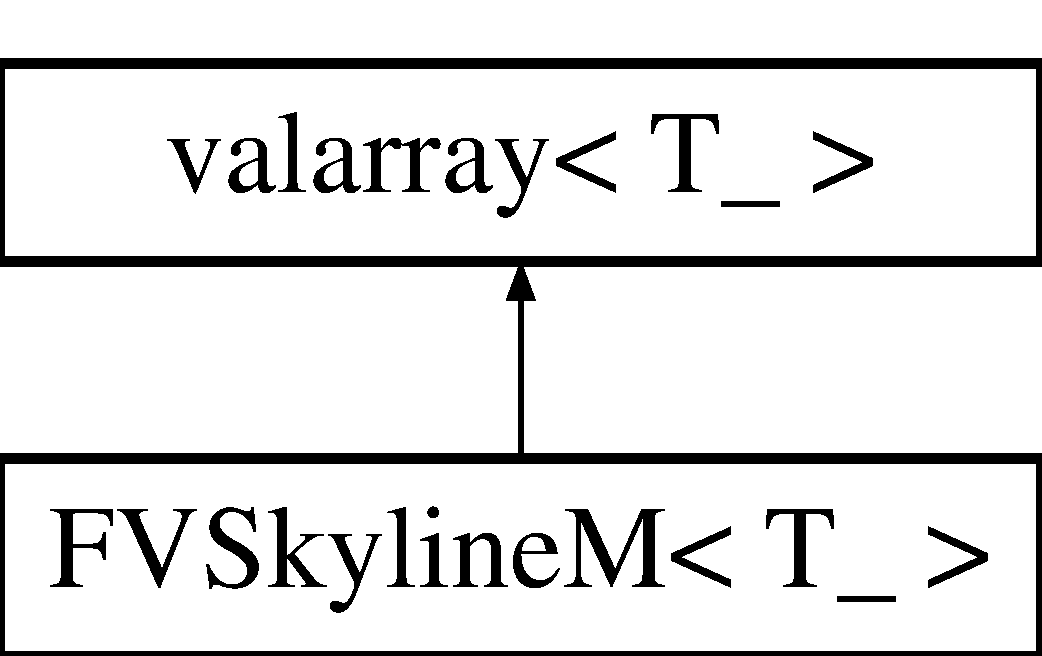
\includegraphics[height=2.000000cm]{d7/d1e/classFVSkylineM}
\end{center}
\end{figure}
\subsubsection*{template$<$class T\_\-$>$ class FVSkylineM$<$ T\_\- $>$}



The documentation for this class was generated from the following file:\begin{DoxyCompactItemize}
\item 
include/\hyperlink{FVSkylineM_8h}{FVSkylineM.h}\end{DoxyCompactItemize}

\hypertarget{classFVSparseM}{
\section{FVSparseM$<$ T\_\- $>$ Class Template Reference}
\label{d2/d4d/classFVSparseM}\index{FVSparseM@{FVSparseM}}
}


{\ttfamily \#include $<$FVSparseM.h$>$}

\subsection*{Public Member Functions}
\begin{DoxyCompactItemize}
\item 
\hyperlink{classFVSparseM_a04619c49ecf6808288fc10d0aaad70e1}{FVSparseM} ()
\item 
\hyperlink{classFVSparseM_a0df0d4878e3fb5bdae16f941b3154260}{$\sim$FVSparseM} ()
\item 
\hyperlink{classFVSparseM_a7c14fc91b113dd18acba072ba1288553}{FVSparseM} (size\_\-t)
\item 
\hyperlink{classFVSparseM_a0056e1e81f3b707ff99b988af48d0503}{FVSparseM} (size\_\-t, size\_\-t)
\item 
\hyperlink{classFVSparseM_a4c75a856ea17c80c2c2c1ed799711f9d}{FVSparseM} (const \hyperlink{classFVSparseM}{FVSparseM}$<$ T\_\- $>$ \&m)
\item 
size\_\-t \hyperlink{classFVSparseM_ae66137e8cb36be98d9d2bd139d4ac021}{getNbColumns} ()
\item 
size\_\-t \hyperlink{classFVSparseM_a33f9a9828a0dd36b3aac2b519e621247}{getNbRows} ()
\item 
size\_\-t \hyperlink{classFVSparseM_a600073d563962412f8873bb598d52be7}{getLength} ()
\item 
void \hyperlink{classFVSparseM_a572d8018b3c8e381d4a8c924bfae3bc6}{resize} (size\_\-t)
\item 
void \hyperlink{classFVSparseM_aa4d3517d2f731ae2943983293a5b1103}{resize} (size\_\-t, size\_\-t)
\item 
void \hyperlink{classFVSparseM_a5145b2a41ccf168751d1dd9972859e32}{setValue} (size\_\-t i, size\_\-t j, const T\_\- \&val)
\item 
void \hyperlink{classFVSparseM_a53fdc14c5ce8e45b80846954c3cc0fbb}{addValue} (size\_\-t i, size\_\-t j, const T\_\- \&val)
\item 
void \hyperlink{classFVSparseM_a8c644f60a185c582b8eaa259d7b65aea}{resizeAndsetValue} (size\_\-t i, size\_\-t j, const T\_\- \&val)
\item 
T\_\- \hyperlink{classFVSparseM_a89d9927485d8a33c508e8caf871ca117}{getValue} (size\_\-t i, size\_\-t j)
\item 
void \hyperlink{classFVSparseM_a4b148f40a95444d5669406b918ad2f52}{show} ()
\item 
\hyperlink{classFVSparseM}{FVSparseM}$<$ T\_\- $>$ \& \hyperlink{classFVSparseM_af82b4e06becaf94b9a98c445a0bcd2f8}{operator/=} (const T\_\- \&val)
\item 
\hyperlink{classFVSparseM}{FVSparseM}$<$ T\_\- $>$ \& \hyperlink{classFVSparseM_ab7ff4e84f06afbf9b1190381e4fabde2}{operator$\ast$=} (const T\_\- \&val)
\item 
void \hyperlink{classFVSparseM_aa8b4d864372618ec7e35dc7be2dc59ef}{Mult} (const \hyperlink{classFVVect}{FVVect}$<$ T\_\- $>$ \&, \hyperlink{classFVVect}{FVVect}$<$ T\_\- $>$ \&) const 
\item 
void \hyperlink{classFVSparseM_a18ce25ba57af55caad2dac42ae0ca2aa}{TransMult} (const \hyperlink{classFVVect}{FVVect}$<$ T\_\- $>$ \&, \hyperlink{classFVVect}{FVVect}$<$ T\_\- $>$ \&) const 
\end{DoxyCompactItemize}
\subsection*{Data Fields}
\begin{DoxyCompactItemize}
\item 
size\_\-t \hyperlink{classFVSparseM_a4451904bc3a87b7e94ba9967cfe5acc9}{nb\_\-cols}
\item 
size\_\-t \hyperlink{classFVSparseM_a660778a5412448cf6b641e67d1d70011}{nb\_\-rows}
\item 
size\_\-t \hyperlink{classFVSparseM_ae809d5359ac030c60a30a8f0b2294b82}{length}
\item 
std::vector$<$ \hyperlink{FVSparseM_8h_a75e12c6bf84f6847b73ab5ab713bf39c}{Tab\_\-index} $\ast$ $>$ \hyperlink{classFVSparseM_ad5e348a06667f83ce7654e382e90ce57}{row}
\item 
std::vector$<$ \hyperlink{FVSparseM_8h_a75e12c6bf84f6847b73ab5ab713bf39c}{Tab\_\-index} $\ast$ $>$ \hyperlink{classFVSparseM_a075a80b2189de3b24e0c89b98cf4ddb9}{col}
\item 
std::vector$<$ T\_\- $>$ \hyperlink{classFVSparseM_aba6347ed10b77e06dd559a865724cfa6}{a}
\end{DoxyCompactItemize}
\subsubsection*{template$<$class T\_\-$>$ class FVSparseM$<$ T\_\- $>$}



\subsection{Constructor \& Destructor Documentation}
\hypertarget{classFVSparseM_a04619c49ecf6808288fc10d0aaad70e1}{
\index{FVSparseM@{FVSparseM}!FVSparseM@{FVSparseM}}
\index{FVSparseM@{FVSparseM}!FVSparseM@{FVSparseM}}
\subsubsection[{FVSparseM}]{\setlength{\rightskip}{0pt plus 5cm}{\bf FVSparseM} (
\begin{DoxyParamCaption}
{}
\end{DoxyParamCaption}
)}}
\label{d2/d4d/classFVSparseM_a04619c49ecf6808288fc10d0aaad70e1}
\hypertarget{classFVSparseM_a0df0d4878e3fb5bdae16f941b3154260}{
\index{FVSparseM@{FVSparseM}!$\sim$FVSparseM@{$\sim$FVSparseM}}
\index{$\sim$FVSparseM@{$\sim$FVSparseM}!FVSparseM@{FVSparseM}}
\subsubsection[{$\sim$FVSparseM}]{\setlength{\rightskip}{0pt plus 5cm}$\sim${\bf FVSparseM} (
\begin{DoxyParamCaption}
{}
\end{DoxyParamCaption}
)}}
\label{d2/d4d/classFVSparseM_a0df0d4878e3fb5bdae16f941b3154260}
\hypertarget{classFVSparseM_a7c14fc91b113dd18acba072ba1288553}{
\index{FVSparseM@{FVSparseM}!FVSparseM@{FVSparseM}}
\index{FVSparseM@{FVSparseM}!FVSparseM@{FVSparseM}}
\subsubsection[{FVSparseM}]{\setlength{\rightskip}{0pt plus 5cm}{\bf FVSparseM} (
\begin{DoxyParamCaption}
\item[{size\_\-t}]{ size}
\end{DoxyParamCaption}
)}}
\label{d2/d4d/classFVSparseM_a7c14fc91b113dd18acba072ba1288553}
\hypertarget{classFVSparseM_a0056e1e81f3b707ff99b988af48d0503}{
\index{FVSparseM@{FVSparseM}!FVSparseM@{FVSparseM}}
\index{FVSparseM@{FVSparseM}!FVSparseM@{FVSparseM}}
\subsubsection[{FVSparseM}]{\setlength{\rightskip}{0pt plus 5cm}{\bf FVSparseM} (
\begin{DoxyParamCaption}
\item[{size\_\-t}]{ nr, }
\item[{size\_\-t}]{ nc}
\end{DoxyParamCaption}
)}}
\label{d2/d4d/classFVSparseM_a0056e1e81f3b707ff99b988af48d0503}
\hypertarget{classFVSparseM_a4c75a856ea17c80c2c2c1ed799711f9d}{
\index{FVSparseM@{FVSparseM}!FVSparseM@{FVSparseM}}
\index{FVSparseM@{FVSparseM}!FVSparseM@{FVSparseM}}
\subsubsection[{FVSparseM}]{\setlength{\rightskip}{0pt plus 5cm}{\bf FVSparseM} (
\begin{DoxyParamCaption}
\item[{const {\bf FVSparseM}$<$ T\_\- $>$ \&}]{ m}
\end{DoxyParamCaption}
)}}
\label{d2/d4d/classFVSparseM_a4c75a856ea17c80c2c2c1ed799711f9d}


\subsection{Member Function Documentation}
\hypertarget{classFVSparseM_a53fdc14c5ce8e45b80846954c3cc0fbb}{
\index{FVSparseM@{FVSparseM}!addValue@{addValue}}
\index{addValue@{addValue}!FVSparseM@{FVSparseM}}
\subsubsection[{addValue}]{\setlength{\rightskip}{0pt plus 5cm}void addValue (
\begin{DoxyParamCaption}
\item[{size\_\-t}]{ i, }
\item[{size\_\-t}]{ j, }
\item[{const T\_\- \&}]{ val}
\end{DoxyParamCaption}
)}}
\label{d2/d4d/classFVSparseM_a53fdc14c5ce8e45b80846954c3cc0fbb}
\hypertarget{classFVSparseM_a600073d563962412f8873bb598d52be7}{
\index{FVSparseM@{FVSparseM}!getLength@{getLength}}
\index{getLength@{getLength}!FVSparseM@{FVSparseM}}
\subsubsection[{getLength}]{\setlength{\rightskip}{0pt plus 5cm}size\_\-t getLength (
\begin{DoxyParamCaption}
{}
\end{DoxyParamCaption}
)\hspace{0.3cm}{\ttfamily  \mbox{[}inline\mbox{]}}}}
\label{d2/d4d/classFVSparseM_a600073d563962412f8873bb598d52be7}
\hypertarget{classFVSparseM_ae66137e8cb36be98d9d2bd139d4ac021}{
\index{FVSparseM@{FVSparseM}!getNbColumns@{getNbColumns}}
\index{getNbColumns@{getNbColumns}!FVSparseM@{FVSparseM}}
\subsubsection[{getNbColumns}]{\setlength{\rightskip}{0pt plus 5cm}size\_\-t getNbColumns (
\begin{DoxyParamCaption}
{}
\end{DoxyParamCaption}
)\hspace{0.3cm}{\ttfamily  \mbox{[}inline\mbox{]}}}}
\label{d2/d4d/classFVSparseM_ae66137e8cb36be98d9d2bd139d4ac021}
\hypertarget{classFVSparseM_a33f9a9828a0dd36b3aac2b519e621247}{
\index{FVSparseM@{FVSparseM}!getNbRows@{getNbRows}}
\index{getNbRows@{getNbRows}!FVSparseM@{FVSparseM}}
\subsubsection[{getNbRows}]{\setlength{\rightskip}{0pt plus 5cm}size\_\-t getNbRows (
\begin{DoxyParamCaption}
{}
\end{DoxyParamCaption}
)\hspace{0.3cm}{\ttfamily  \mbox{[}inline\mbox{]}}}}
\label{d2/d4d/classFVSparseM_a33f9a9828a0dd36b3aac2b519e621247}
\hypertarget{classFVSparseM_a89d9927485d8a33c508e8caf871ca117}{
\index{FVSparseM@{FVSparseM}!getValue@{getValue}}
\index{getValue@{getValue}!FVSparseM@{FVSparseM}}
\subsubsection[{getValue}]{\setlength{\rightskip}{0pt plus 5cm}T\_\- getValue (
\begin{DoxyParamCaption}
\item[{size\_\-t}]{ i, }
\item[{size\_\-t}]{ j}
\end{DoxyParamCaption}
)}}
\label{d2/d4d/classFVSparseM_a89d9927485d8a33c508e8caf871ca117}
\hypertarget{classFVSparseM_aa8b4d864372618ec7e35dc7be2dc59ef}{
\index{FVSparseM@{FVSparseM}!Mult@{Mult}}
\index{Mult@{Mult}!FVSparseM@{FVSparseM}}
\subsubsection[{Mult}]{\setlength{\rightskip}{0pt plus 5cm}void Mult (
\begin{DoxyParamCaption}
\item[{const {\bf FVVect}$<$ T\_\- $>$ \&}]{ x, }
\item[{{\bf FVVect}$<$ T\_\- $>$ \&}]{ y}
\end{DoxyParamCaption}
) const}}
\label{d2/d4d/classFVSparseM_aa8b4d864372618ec7e35dc7be2dc59ef}
\hypertarget{classFVSparseM_ab7ff4e84f06afbf9b1190381e4fabde2}{
\index{FVSparseM@{FVSparseM}!operator$\ast$=@{operator$\ast$=}}
\index{operator$\ast$=@{operator$\ast$=}!FVSparseM@{FVSparseM}}
\subsubsection[{operator$\ast$=}]{\setlength{\rightskip}{0pt plus 5cm}{\bf FVSparseM}$<$ T\_\- $>$ \& operator$\ast$= (
\begin{DoxyParamCaption}
\item[{const T\_\- \&}]{ val}
\end{DoxyParamCaption}
)}}
\label{d2/d4d/classFVSparseM_ab7ff4e84f06afbf9b1190381e4fabde2}
\hypertarget{classFVSparseM_af82b4e06becaf94b9a98c445a0bcd2f8}{
\index{FVSparseM@{FVSparseM}!operator/=@{operator/=}}
\index{operator/=@{operator/=}!FVSparseM@{FVSparseM}}
\subsubsection[{operator/=}]{\setlength{\rightskip}{0pt plus 5cm}{\bf FVSparseM}$<$ T\_\- $>$ \& operator/= (
\begin{DoxyParamCaption}
\item[{const T\_\- \&}]{ val}
\end{DoxyParamCaption}
)}}
\label{d2/d4d/classFVSparseM_af82b4e06becaf94b9a98c445a0bcd2f8}
\hypertarget{classFVSparseM_a572d8018b3c8e381d4a8c924bfae3bc6}{
\index{FVSparseM@{FVSparseM}!resize@{resize}}
\index{resize@{resize}!FVSparseM@{FVSparseM}}
\subsubsection[{resize}]{\setlength{\rightskip}{0pt plus 5cm}void resize (
\begin{DoxyParamCaption}
\item[{size\_\-t}]{ size}
\end{DoxyParamCaption}
)}}
\label{d2/d4d/classFVSparseM_a572d8018b3c8e381d4a8c924bfae3bc6}
\hypertarget{classFVSparseM_aa4d3517d2f731ae2943983293a5b1103}{
\index{FVSparseM@{FVSparseM}!resize@{resize}}
\index{resize@{resize}!FVSparseM@{FVSparseM}}
\subsubsection[{resize}]{\setlength{\rightskip}{0pt plus 5cm}void resize (
\begin{DoxyParamCaption}
\item[{size\_\-t}]{ nr, }
\item[{size\_\-t}]{ nc}
\end{DoxyParamCaption}
)}}
\label{d2/d4d/classFVSparseM_aa4d3517d2f731ae2943983293a5b1103}
\hypertarget{classFVSparseM_a8c644f60a185c582b8eaa259d7b65aea}{
\index{FVSparseM@{FVSparseM}!resizeAndsetValue@{resizeAndsetValue}}
\index{resizeAndsetValue@{resizeAndsetValue}!FVSparseM@{FVSparseM}}
\subsubsection[{resizeAndsetValue}]{\setlength{\rightskip}{0pt plus 5cm}void resizeAndsetValue (
\begin{DoxyParamCaption}
\item[{size\_\-t}]{ i, }
\item[{size\_\-t}]{ j, }
\item[{const T\_\- \&}]{ val}
\end{DoxyParamCaption}
)}}
\label{d2/d4d/classFVSparseM_a8c644f60a185c582b8eaa259d7b65aea}
\hypertarget{classFVSparseM_a5145b2a41ccf168751d1dd9972859e32}{
\index{FVSparseM@{FVSparseM}!setValue@{setValue}}
\index{setValue@{setValue}!FVSparseM@{FVSparseM}}
\subsubsection[{setValue}]{\setlength{\rightskip}{0pt plus 5cm}void setValue (
\begin{DoxyParamCaption}
\item[{size\_\-t}]{ i, }
\item[{size\_\-t}]{ j, }
\item[{const T\_\- \&}]{ val}
\end{DoxyParamCaption}
)}}
\label{d2/d4d/classFVSparseM_a5145b2a41ccf168751d1dd9972859e32}
\hypertarget{classFVSparseM_a4b148f40a95444d5669406b918ad2f52}{
\index{FVSparseM@{FVSparseM}!show@{show}}
\index{show@{show}!FVSparseM@{FVSparseM}}
\subsubsection[{show}]{\setlength{\rightskip}{0pt plus 5cm}void show (
\begin{DoxyParamCaption}
{}
\end{DoxyParamCaption}
)}}
\label{d2/d4d/classFVSparseM_a4b148f40a95444d5669406b918ad2f52}
\hypertarget{classFVSparseM_a18ce25ba57af55caad2dac42ae0ca2aa}{
\index{FVSparseM@{FVSparseM}!TransMult@{TransMult}}
\index{TransMult@{TransMult}!FVSparseM@{FVSparseM}}
\subsubsection[{TransMult}]{\setlength{\rightskip}{0pt plus 5cm}void TransMult (
\begin{DoxyParamCaption}
\item[{const {\bf FVVect}$<$ T\_\- $>$ \&}]{ x, }
\item[{{\bf FVVect}$<$ T\_\- $>$ \&}]{ y}
\end{DoxyParamCaption}
) const}}
\label{d2/d4d/classFVSparseM_a18ce25ba57af55caad2dac42ae0ca2aa}


\subsection{Field Documentation}
\hypertarget{classFVSparseM_aba6347ed10b77e06dd559a865724cfa6}{
\index{FVSparseM@{FVSparseM}!a@{a}}
\index{a@{a}!FVSparseM@{FVSparseM}}
\subsubsection[{a}]{\setlength{\rightskip}{0pt plus 5cm}std::vector$<$T\_\-$>$ {\bf a}}}
\label{d2/d4d/classFVSparseM_aba6347ed10b77e06dd559a865724cfa6}
\hypertarget{classFVSparseM_a075a80b2189de3b24e0c89b98cf4ddb9}{
\index{FVSparseM@{FVSparseM}!col@{col}}
\index{col@{col}!FVSparseM@{FVSparseM}}
\subsubsection[{col}]{\setlength{\rightskip}{0pt plus 5cm}std::vector$<${\bf Tab\_\-index} $\ast$$>$ {\bf col}}}
\label{d2/d4d/classFVSparseM_a075a80b2189de3b24e0c89b98cf4ddb9}
\hypertarget{classFVSparseM_ae809d5359ac030c60a30a8f0b2294b82}{
\index{FVSparseM@{FVSparseM}!length@{length}}
\index{length@{length}!FVSparseM@{FVSparseM}}
\subsubsection[{length}]{\setlength{\rightskip}{0pt plus 5cm}size\_\-t {\bf length}}}
\label{d2/d4d/classFVSparseM_ae809d5359ac030c60a30a8f0b2294b82}
\hypertarget{classFVSparseM_a4451904bc3a87b7e94ba9967cfe5acc9}{
\index{FVSparseM@{FVSparseM}!nb\_\-cols@{nb\_\-cols}}
\index{nb\_\-cols@{nb\_\-cols}!FVSparseM@{FVSparseM}}
\subsubsection[{nb\_\-cols}]{\setlength{\rightskip}{0pt plus 5cm}size\_\-t {\bf nb\_\-cols}}}
\label{d2/d4d/classFVSparseM_a4451904bc3a87b7e94ba9967cfe5acc9}
\hypertarget{classFVSparseM_a660778a5412448cf6b641e67d1d70011}{
\index{FVSparseM@{FVSparseM}!nb\_\-rows@{nb\_\-rows}}
\index{nb\_\-rows@{nb\_\-rows}!FVSparseM@{FVSparseM}}
\subsubsection[{nb\_\-rows}]{\setlength{\rightskip}{0pt plus 5cm}size\_\-t {\bf nb\_\-rows}}}
\label{d2/d4d/classFVSparseM_a660778a5412448cf6b641e67d1d70011}
\hypertarget{classFVSparseM_ad5e348a06667f83ce7654e382e90ce57}{
\index{FVSparseM@{FVSparseM}!row@{row}}
\index{row@{row}!FVSparseM@{FVSparseM}}
\subsubsection[{row}]{\setlength{\rightskip}{0pt plus 5cm}std::vector$<${\bf Tab\_\-index} $\ast$$>$ {\bf row}}}
\label{d2/d4d/classFVSparseM_ad5e348a06667f83ce7654e382e90ce57}


The documentation for this class was generated from the following file:\begin{DoxyCompactItemize}
\item 
include/\hyperlink{FVSparseM_8h}{FVSparseM.h}\end{DoxyCompactItemize}

\hypertarget{classFVStencil}{
\section{FVStencil Class Reference}
\label{d3/d29/classFVStencil}\index{FVStencil@{FVStencil}}
}


{\ttfamily \#include $<$FVStencil.h$>$}

\subsection*{Public Member Functions}
\begin{DoxyCompactItemize}
\item 
\hyperlink{classFVStencil_abe323f23f20253e4f0732f76519d611d}{FVStencil} ()
\item 
\hyperlink{classFVStencil_ad9ce349d4bd2d08d970943e47e0fc3fb}{$\sim$FVStencil} ()
\item 
\hyperlink{classFVStencil_acc34bddee6d41971ae7b4425254bb5a3}{FVStencil} (const \hyperlink{classFVStencil}{FVStencil} \&st)
\item 
void $\ast$ \hyperlink{classFVStencil_afbfae7a493f514f96af208b73d1336b2}{beginGeometry} ()
\item 
void $\ast$ \hyperlink{classFVStencil_a484f74785f318a09811aa0ecc7e40150}{nextGeometry} ()
\item 
void $\ast$ \hyperlink{classFVStencil_ac215cf3defe013cbed6a69d1fac9787a}{getGeometry} (size\_\-t i)
\item 
size\_\-t \hyperlink{classFVStencil_a74ab61efe1dd84c16c6f76179fb6f76c}{getType} ()
\item 
size\_\-t \hyperlink{classFVStencil_ab00c0a65e8424f5640f369bbf6f8ccea}{getIndex} ()
\item 
size\_\-t \hyperlink{classFVStencil_a6b6dda042f3f8a07b9789cb35b719f20}{getReferenceType} ()
\item 
size\_\-t \hyperlink{classFVStencil_a456fe2c00099965cd8b4597187f5c1a3}{getType} (size\_\-t i)
\item 
void $\ast$ \hyperlink{classFVStencil_a270d27e05efea4b490b7d8fa7bcf379d}{getReferenceGeometry} ()
\item 
size\_\-t \hyperlink{classFVStencil_afc6b28968b6632bd16c8a1ae5d1f3ca2}{getNbGeometry} ()
\item 
void \hyperlink{classFVStencil_a2bbe646c052baf99f04a367ef6031d74}{clean} ()
\item 
void \hyperlink{classFVStencil_a4b148f40a95444d5669406b918ad2f52}{show} ()
\item 
void \hyperlink{classFVStencil_af0785e8c3b770acb028b0e71bb7b210e}{addStencil} (\hyperlink{classFVVertex1D}{FVVertex1D} $\ast$ptr)
\item 
void \hyperlink{classFVStencil_a99bceb22726fcc1b5ef089248dcc9166}{setReferenceGeometry} (\hyperlink{classFVVertex1D}{FVVertex1D} $\ast$ptr)
\item 
void \hyperlink{classFVStencil_aab21f08ad1f0558c56004122f2c64f98}{addStencil} (\hyperlink{classFVVertex2D}{FVVertex2D} $\ast$ptr)
\item 
void \hyperlink{classFVStencil_a2a114a8cce549499c9689315b8d2c4cf}{setReferenceGeometry} (\hyperlink{classFVVertex2D}{FVVertex2D} $\ast$ptr)
\item 
void \hyperlink{classFVStencil_ad059e11d270b826f2f01dd90c23fd012}{addStencil} (\hyperlink{classFVVertex3D}{FVVertex3D} $\ast$ptr)
\item 
void \hyperlink{classFVStencil_a61055cf4bb03435a6963051a10772c42}{setReferenceGeometry} (\hyperlink{classFVVertex3D}{FVVertex3D} $\ast$ptr)
\item 
void \hyperlink{classFVStencil_ad840c62f1333c72eb216e66c6e057979}{addStencil} (\hyperlink{classFVCell1D}{FVCell1D} $\ast$ptr)
\item 
void \hyperlink{classFVStencil_a0eabbf88ec0417f4edf00d260630512b}{setReferenceGeometry} (\hyperlink{classFVCell1D}{FVCell1D} $\ast$ptr)
\item 
void \hyperlink{classFVStencil_aa353de8869c3168238441ee2ea022b25}{addStencil} (\hyperlink{classFVCell2D}{FVCell2D} $\ast$ptr)
\item 
void \hyperlink{classFVStencil_a9584ca9b8b12d456a24992af7d9b3502}{setReferenceGeometry} (\hyperlink{classFVCell2D}{FVCell2D} $\ast$ptr)
\item 
void \hyperlink{classFVStencil_a5e51c58a3cd246d5d6c1556f724d0eda}{addStencil} (\hyperlink{classFVCell3D}{FVCell3D} $\ast$ptr)
\item 
void \hyperlink{classFVStencil_ab48ae71ad38034649303834c804501c1}{setReferenceGeometry} (\hyperlink{classFVCell3D}{FVCell3D} $\ast$ptr)
\item 
void \hyperlink{classFVStencil_a8c8c76b8a1c6f6bb79f2db50a3f5e951}{addStencil} (\hyperlink{classFVEdge2D}{FVEdge2D} $\ast$ptr)
\item 
void \hyperlink{classFVStencil_a0dfb63f3f0d2f6a64134c5fd14d56ef3}{setReferenceGeometry} (\hyperlink{classFVEdge2D}{FVEdge2D} $\ast$ptr)
\item 
void \hyperlink{classFVStencil_a4fcafa6a6e90124be6e386eee452c384}{addStencil} (\hyperlink{classFVEdge3D}{FVEdge3D} $\ast$ptr)
\item 
void \hyperlink{classFVStencil_af5c5c9120d56c6948abb0a1fbb4d34b0}{setReferenceGeometry} (\hyperlink{classFVEdge3D}{FVEdge3D} $\ast$ptr)
\item 
void \hyperlink{classFVStencil_a3edafd7e6321ad197b92e2a5e36ab2ab}{addStencil} (\hyperlink{classFVFace3D}{FVFace3D} $\ast$ptr)
\item 
void \hyperlink{classFVStencil_aee6c45898f401346fdaa402792ba4f77}{setReferenceGeometry} (\hyperlink{classFVFace3D}{FVFace3D} $\ast$ptr)
\end{DoxyCompactItemize}


\subsection{Constructor \& Destructor Documentation}
\hypertarget{classFVStencil_abe323f23f20253e4f0732f76519d611d}{
\index{FVStencil@{FVStencil}!FVStencil@{FVStencil}}
\index{FVStencil@{FVStencil}!FVStencil@{FVStencil}}
\subsubsection[{FVStencil}]{\setlength{\rightskip}{0pt plus 5cm}{\bf FVStencil} (
\begin{DoxyParamCaption}
{}
\end{DoxyParamCaption}
)\hspace{0.3cm}{\ttfamily  \mbox{[}inline\mbox{]}}}}
\label{d3/d29/classFVStencil_abe323f23f20253e4f0732f76519d611d}
\hypertarget{classFVStencil_ad9ce349d4bd2d08d970943e47e0fc3fb}{
\index{FVStencil@{FVStencil}!$\sim$FVStencil@{$\sim$FVStencil}}
\index{$\sim$FVStencil@{$\sim$FVStencil}!FVStencil@{FVStencil}}
\subsubsection[{$\sim$FVStencil}]{\setlength{\rightskip}{0pt plus 5cm}$\sim${\bf FVStencil} (
\begin{DoxyParamCaption}
{}
\end{DoxyParamCaption}
)\hspace{0.3cm}{\ttfamily  \mbox{[}inline\mbox{]}}}}
\label{d3/d29/classFVStencil_ad9ce349d4bd2d08d970943e47e0fc3fb}
\hypertarget{classFVStencil_acc34bddee6d41971ae7b4425254bb5a3}{
\index{FVStencil@{FVStencil}!FVStencil@{FVStencil}}
\index{FVStencil@{FVStencil}!FVStencil@{FVStencil}}
\subsubsection[{FVStencil}]{\setlength{\rightskip}{0pt plus 5cm}{\bf FVStencil} (
\begin{DoxyParamCaption}
\item[{const {\bf FVStencil} \&}]{ st}
\end{DoxyParamCaption}
)}}
\label{d3/d29/classFVStencil_acc34bddee6d41971ae7b4425254bb5a3}


\subsection{Member Function Documentation}
\hypertarget{classFVStencil_af0785e8c3b770acb028b0e71bb7b210e}{
\index{FVStencil@{FVStencil}!addStencil@{addStencil}}
\index{addStencil@{addStencil}!FVStencil@{FVStencil}}
\subsubsection[{addStencil}]{\setlength{\rightskip}{0pt plus 5cm}void addStencil (
\begin{DoxyParamCaption}
\item[{{\bf FVVertex1D} $\ast$}]{ ptr}
\end{DoxyParamCaption}
)}}
\label{d3/d29/classFVStencil_af0785e8c3b770acb028b0e71bb7b210e}
\hypertarget{classFVStencil_ad059e11d270b826f2f01dd90c23fd012}{
\index{FVStencil@{FVStencil}!addStencil@{addStencil}}
\index{addStencil@{addStencil}!FVStencil@{FVStencil}}
\subsubsection[{addStencil}]{\setlength{\rightskip}{0pt plus 5cm}void addStencil (
\begin{DoxyParamCaption}
\item[{{\bf FVVertex3D} $\ast$}]{ ptr}
\end{DoxyParamCaption}
)}}
\label{d3/d29/classFVStencil_ad059e11d270b826f2f01dd90c23fd012}
\hypertarget{classFVStencil_ad840c62f1333c72eb216e66c6e057979}{
\index{FVStencil@{FVStencil}!addStencil@{addStencil}}
\index{addStencil@{addStencil}!FVStencil@{FVStencil}}
\subsubsection[{addStencil}]{\setlength{\rightskip}{0pt plus 5cm}void addStencil (
\begin{DoxyParamCaption}
\item[{{\bf FVCell1D} $\ast$}]{ ptr}
\end{DoxyParamCaption}
)}}
\label{d3/d29/classFVStencil_ad840c62f1333c72eb216e66c6e057979}
\hypertarget{classFVStencil_aa353de8869c3168238441ee2ea022b25}{
\index{FVStencil@{FVStencil}!addStencil@{addStencil}}
\index{addStencil@{addStencil}!FVStencil@{FVStencil}}
\subsubsection[{addStencil}]{\setlength{\rightskip}{0pt plus 5cm}void addStencil (
\begin{DoxyParamCaption}
\item[{{\bf FVCell2D} $\ast$}]{ ptr}
\end{DoxyParamCaption}
)}}
\label{d3/d29/classFVStencil_aa353de8869c3168238441ee2ea022b25}
\hypertarget{classFVStencil_a5e51c58a3cd246d5d6c1556f724d0eda}{
\index{FVStencil@{FVStencil}!addStencil@{addStencil}}
\index{addStencil@{addStencil}!FVStencil@{FVStencil}}
\subsubsection[{addStencil}]{\setlength{\rightskip}{0pt plus 5cm}void addStencil (
\begin{DoxyParamCaption}
\item[{{\bf FVCell3D} $\ast$}]{ ptr}
\end{DoxyParamCaption}
)}}
\label{d3/d29/classFVStencil_a5e51c58a3cd246d5d6c1556f724d0eda}
\hypertarget{classFVStencil_aab21f08ad1f0558c56004122f2c64f98}{
\index{FVStencil@{FVStencil}!addStencil@{addStencil}}
\index{addStencil@{addStencil}!FVStencil@{FVStencil}}
\subsubsection[{addStencil}]{\setlength{\rightskip}{0pt plus 5cm}void addStencil (
\begin{DoxyParamCaption}
\item[{{\bf FVVertex2D} $\ast$}]{ ptr}
\end{DoxyParamCaption}
)}}
\label{d3/d29/classFVStencil_aab21f08ad1f0558c56004122f2c64f98}
\hypertarget{classFVStencil_a8c8c76b8a1c6f6bb79f2db50a3f5e951}{
\index{FVStencil@{FVStencil}!addStencil@{addStencil}}
\index{addStencil@{addStencil}!FVStencil@{FVStencil}}
\subsubsection[{addStencil}]{\setlength{\rightskip}{0pt plus 5cm}void addStencil (
\begin{DoxyParamCaption}
\item[{{\bf FVEdge2D} $\ast$}]{ ptr}
\end{DoxyParamCaption}
)}}
\label{d3/d29/classFVStencil_a8c8c76b8a1c6f6bb79f2db50a3f5e951}
\hypertarget{classFVStencil_a4fcafa6a6e90124be6e386eee452c384}{
\index{FVStencil@{FVStencil}!addStencil@{addStencil}}
\index{addStencil@{addStencil}!FVStencil@{FVStencil}}
\subsubsection[{addStencil}]{\setlength{\rightskip}{0pt plus 5cm}void addStencil (
\begin{DoxyParamCaption}
\item[{{\bf FVEdge3D} $\ast$}]{ ptr}
\end{DoxyParamCaption}
)}}
\label{d3/d29/classFVStencil_a4fcafa6a6e90124be6e386eee452c384}
\hypertarget{classFVStencil_a3edafd7e6321ad197b92e2a5e36ab2ab}{
\index{FVStencil@{FVStencil}!addStencil@{addStencil}}
\index{addStencil@{addStencil}!FVStencil@{FVStencil}}
\subsubsection[{addStencil}]{\setlength{\rightskip}{0pt plus 5cm}void addStencil (
\begin{DoxyParamCaption}
\item[{{\bf FVFace3D} $\ast$}]{ ptr}
\end{DoxyParamCaption}
)}}
\label{d3/d29/classFVStencil_a3edafd7e6321ad197b92e2a5e36ab2ab}
\hypertarget{classFVStencil_afbfae7a493f514f96af208b73d1336b2}{
\index{FVStencil@{FVStencil}!beginGeometry@{beginGeometry}}
\index{beginGeometry@{beginGeometry}!FVStencil@{FVStencil}}
\subsubsection[{beginGeometry}]{\setlength{\rightskip}{0pt plus 5cm}void$\ast$ beginGeometry (
\begin{DoxyParamCaption}
{}
\end{DoxyParamCaption}
)\hspace{0.3cm}{\ttfamily  \mbox{[}inline\mbox{]}}}}
\label{d3/d29/classFVStencil_afbfae7a493f514f96af208b73d1336b2}
\hypertarget{classFVStencil_a2bbe646c052baf99f04a367ef6031d74}{
\index{FVStencil@{FVStencil}!clean@{clean}}
\index{clean@{clean}!FVStencil@{FVStencil}}
\subsubsection[{clean}]{\setlength{\rightskip}{0pt plus 5cm}void clean (
\begin{DoxyParamCaption}
{}
\end{DoxyParamCaption}
)\hspace{0.3cm}{\ttfamily  \mbox{[}inline\mbox{]}}}}
\label{d3/d29/classFVStencil_a2bbe646c052baf99f04a367ef6031d74}
\hypertarget{classFVStencil_ac215cf3defe013cbed6a69d1fac9787a}{
\index{FVStencil@{FVStencil}!getGeometry@{getGeometry}}
\index{getGeometry@{getGeometry}!FVStencil@{FVStencil}}
\subsubsection[{getGeometry}]{\setlength{\rightskip}{0pt plus 5cm}void$\ast$ getGeometry (
\begin{DoxyParamCaption}
\item[{size\_\-t}]{ i}
\end{DoxyParamCaption}
)\hspace{0.3cm}{\ttfamily  \mbox{[}inline\mbox{]}}}}
\label{d3/d29/classFVStencil_ac215cf3defe013cbed6a69d1fac9787a}
\hypertarget{classFVStencil_ab00c0a65e8424f5640f369bbf6f8ccea}{
\index{FVStencil@{FVStencil}!getIndex@{getIndex}}
\index{getIndex@{getIndex}!FVStencil@{FVStencil}}
\subsubsection[{getIndex}]{\setlength{\rightskip}{0pt plus 5cm}size\_\-t getIndex (
\begin{DoxyParamCaption}
{}
\end{DoxyParamCaption}
)\hspace{0.3cm}{\ttfamily  \mbox{[}inline\mbox{]}}}}
\label{d3/d29/classFVStencil_ab00c0a65e8424f5640f369bbf6f8ccea}
\hypertarget{classFVStencil_afc6b28968b6632bd16c8a1ae5d1f3ca2}{
\index{FVStencil@{FVStencil}!getNbGeometry@{getNbGeometry}}
\index{getNbGeometry@{getNbGeometry}!FVStencil@{FVStencil}}
\subsubsection[{getNbGeometry}]{\setlength{\rightskip}{0pt plus 5cm}size\_\-t getNbGeometry (
\begin{DoxyParamCaption}
{}
\end{DoxyParamCaption}
)\hspace{0.3cm}{\ttfamily  \mbox{[}inline\mbox{]}}}}
\label{d3/d29/classFVStencil_afc6b28968b6632bd16c8a1ae5d1f3ca2}
\hypertarget{classFVStencil_a270d27e05efea4b490b7d8fa7bcf379d}{
\index{FVStencil@{FVStencil}!getReferenceGeometry@{getReferenceGeometry}}
\index{getReferenceGeometry@{getReferenceGeometry}!FVStencil@{FVStencil}}
\subsubsection[{getReferenceGeometry}]{\setlength{\rightskip}{0pt plus 5cm}void$\ast$ getReferenceGeometry (
\begin{DoxyParamCaption}
{}
\end{DoxyParamCaption}
)\hspace{0.3cm}{\ttfamily  \mbox{[}inline\mbox{]}}}}
\label{d3/d29/classFVStencil_a270d27e05efea4b490b7d8fa7bcf379d}
\hypertarget{classFVStencil_a6b6dda042f3f8a07b9789cb35b719f20}{
\index{FVStencil@{FVStencil}!getReferenceType@{getReferenceType}}
\index{getReferenceType@{getReferenceType}!FVStencil@{FVStencil}}
\subsubsection[{getReferenceType}]{\setlength{\rightskip}{0pt plus 5cm}size\_\-t getReferenceType (
\begin{DoxyParamCaption}
{}
\end{DoxyParamCaption}
)\hspace{0.3cm}{\ttfamily  \mbox{[}inline\mbox{]}}}}
\label{d3/d29/classFVStencil_a6b6dda042f3f8a07b9789cb35b719f20}
\hypertarget{classFVStencil_a74ab61efe1dd84c16c6f76179fb6f76c}{
\index{FVStencil@{FVStencil}!getType@{getType}}
\index{getType@{getType}!FVStencil@{FVStencil}}
\subsubsection[{getType}]{\setlength{\rightskip}{0pt plus 5cm}size\_\-t getType (
\begin{DoxyParamCaption}
{}
\end{DoxyParamCaption}
)\hspace{0.3cm}{\ttfamily  \mbox{[}inline\mbox{]}}}}
\label{d3/d29/classFVStencil_a74ab61efe1dd84c16c6f76179fb6f76c}
\hypertarget{classFVStencil_a456fe2c00099965cd8b4597187f5c1a3}{
\index{FVStencil@{FVStencil}!getType@{getType}}
\index{getType@{getType}!FVStencil@{FVStencil}}
\subsubsection[{getType}]{\setlength{\rightskip}{0pt plus 5cm}size\_\-t getType (
\begin{DoxyParamCaption}
\item[{size\_\-t}]{ i}
\end{DoxyParamCaption}
)\hspace{0.3cm}{\ttfamily  \mbox{[}inline\mbox{]}}}}
\label{d3/d29/classFVStencil_a456fe2c00099965cd8b4597187f5c1a3}
\hypertarget{classFVStencil_a484f74785f318a09811aa0ecc7e40150}{
\index{FVStencil@{FVStencil}!nextGeometry@{nextGeometry}}
\index{nextGeometry@{nextGeometry}!FVStencil@{FVStencil}}
\subsubsection[{nextGeometry}]{\setlength{\rightskip}{0pt plus 5cm}void$\ast$ nextGeometry (
\begin{DoxyParamCaption}
{}
\end{DoxyParamCaption}
)\hspace{0.3cm}{\ttfamily  \mbox{[}inline\mbox{]}}}}
\label{d3/d29/classFVStencil_a484f74785f318a09811aa0ecc7e40150}
\hypertarget{classFVStencil_a99bceb22726fcc1b5ef089248dcc9166}{
\index{FVStencil@{FVStencil}!setReferenceGeometry@{setReferenceGeometry}}
\index{setReferenceGeometry@{setReferenceGeometry}!FVStencil@{FVStencil}}
\subsubsection[{setReferenceGeometry}]{\setlength{\rightskip}{0pt plus 5cm}void setReferenceGeometry (
\begin{DoxyParamCaption}
\item[{{\bf FVVertex1D} $\ast$}]{ ptr}
\end{DoxyParamCaption}
)}}
\label{d3/d29/classFVStencil_a99bceb22726fcc1b5ef089248dcc9166}
\hypertarget{classFVStencil_a9584ca9b8b12d456a24992af7d9b3502}{
\index{FVStencil@{FVStencil}!setReferenceGeometry@{setReferenceGeometry}}
\index{setReferenceGeometry@{setReferenceGeometry}!FVStencil@{FVStencil}}
\subsubsection[{setReferenceGeometry}]{\setlength{\rightskip}{0pt plus 5cm}void setReferenceGeometry (
\begin{DoxyParamCaption}
\item[{{\bf FVCell2D} $\ast$}]{ ptr}
\end{DoxyParamCaption}
)}}
\label{d3/d29/classFVStencil_a9584ca9b8b12d456a24992af7d9b3502}
\hypertarget{classFVStencil_aee6c45898f401346fdaa402792ba4f77}{
\index{FVStencil@{FVStencil}!setReferenceGeometry@{setReferenceGeometry}}
\index{setReferenceGeometry@{setReferenceGeometry}!FVStencil@{FVStencil}}
\subsubsection[{setReferenceGeometry}]{\setlength{\rightskip}{0pt plus 5cm}void setReferenceGeometry (
\begin{DoxyParamCaption}
\item[{{\bf FVFace3D} $\ast$}]{ ptr}
\end{DoxyParamCaption}
)}}
\label{d3/d29/classFVStencil_aee6c45898f401346fdaa402792ba4f77}
\hypertarget{classFVStencil_a0dfb63f3f0d2f6a64134c5fd14d56ef3}{
\index{FVStencil@{FVStencil}!setReferenceGeometry@{setReferenceGeometry}}
\index{setReferenceGeometry@{setReferenceGeometry}!FVStencil@{FVStencil}}
\subsubsection[{setReferenceGeometry}]{\setlength{\rightskip}{0pt plus 5cm}void setReferenceGeometry (
\begin{DoxyParamCaption}
\item[{{\bf FVEdge2D} $\ast$}]{ ptr}
\end{DoxyParamCaption}
)}}
\label{d3/d29/classFVStencil_a0dfb63f3f0d2f6a64134c5fd14d56ef3}
\hypertarget{classFVStencil_ab48ae71ad38034649303834c804501c1}{
\index{FVStencil@{FVStencil}!setReferenceGeometry@{setReferenceGeometry}}
\index{setReferenceGeometry@{setReferenceGeometry}!FVStencil@{FVStencil}}
\subsubsection[{setReferenceGeometry}]{\setlength{\rightskip}{0pt plus 5cm}void setReferenceGeometry (
\begin{DoxyParamCaption}
\item[{{\bf FVCell3D} $\ast$}]{ ptr}
\end{DoxyParamCaption}
)}}
\label{d3/d29/classFVStencil_ab48ae71ad38034649303834c804501c1}
\hypertarget{classFVStencil_a0eabbf88ec0417f4edf00d260630512b}{
\index{FVStencil@{FVStencil}!setReferenceGeometry@{setReferenceGeometry}}
\index{setReferenceGeometry@{setReferenceGeometry}!FVStencil@{FVStencil}}
\subsubsection[{setReferenceGeometry}]{\setlength{\rightskip}{0pt plus 5cm}void setReferenceGeometry (
\begin{DoxyParamCaption}
\item[{{\bf FVCell1D} $\ast$}]{ ptr}
\end{DoxyParamCaption}
)}}
\label{d3/d29/classFVStencil_a0eabbf88ec0417f4edf00d260630512b}
\hypertarget{classFVStencil_af5c5c9120d56c6948abb0a1fbb4d34b0}{
\index{FVStencil@{FVStencil}!setReferenceGeometry@{setReferenceGeometry}}
\index{setReferenceGeometry@{setReferenceGeometry}!FVStencil@{FVStencil}}
\subsubsection[{setReferenceGeometry}]{\setlength{\rightskip}{0pt plus 5cm}void setReferenceGeometry (
\begin{DoxyParamCaption}
\item[{{\bf FVEdge3D} $\ast$}]{ ptr}
\end{DoxyParamCaption}
)}}
\label{d3/d29/classFVStencil_af5c5c9120d56c6948abb0a1fbb4d34b0}
\hypertarget{classFVStencil_a61055cf4bb03435a6963051a10772c42}{
\index{FVStencil@{FVStencil}!setReferenceGeometry@{setReferenceGeometry}}
\index{setReferenceGeometry@{setReferenceGeometry}!FVStencil@{FVStencil}}
\subsubsection[{setReferenceGeometry}]{\setlength{\rightskip}{0pt plus 5cm}void setReferenceGeometry (
\begin{DoxyParamCaption}
\item[{{\bf FVVertex3D} $\ast$}]{ ptr}
\end{DoxyParamCaption}
)}}
\label{d3/d29/classFVStencil_a61055cf4bb03435a6963051a10772c42}
\hypertarget{classFVStencil_a2a114a8cce549499c9689315b8d2c4cf}{
\index{FVStencil@{FVStencil}!setReferenceGeometry@{setReferenceGeometry}}
\index{setReferenceGeometry@{setReferenceGeometry}!FVStencil@{FVStencil}}
\subsubsection[{setReferenceGeometry}]{\setlength{\rightskip}{0pt plus 5cm}void setReferenceGeometry (
\begin{DoxyParamCaption}
\item[{{\bf FVVertex2D} $\ast$}]{ ptr}
\end{DoxyParamCaption}
)}}
\label{d3/d29/classFVStencil_a2a114a8cce549499c9689315b8d2c4cf}
\hypertarget{classFVStencil_a4b148f40a95444d5669406b918ad2f52}{
\index{FVStencil@{FVStencil}!show@{show}}
\index{show@{show}!FVStencil@{FVStencil}}
\subsubsection[{show}]{\setlength{\rightskip}{0pt plus 5cm}void show (
\begin{DoxyParamCaption}
{}
\end{DoxyParamCaption}
)}}
\label{d3/d29/classFVStencil_a4b148f40a95444d5669406b918ad2f52}


The documentation for this class was generated from the following file:\begin{DoxyCompactItemize}
\item 
include/\hyperlink{FVStencil_8h}{FVStencil.h}\end{DoxyCompactItemize}

\hypertarget{classFVVect}{
\section{FVVect$<$ T\_\- $>$ Class Template Reference}
\label{da/d83/classFVVect}\index{FVVect@{FVVect}}
}


{\ttfamily \#include $<$FVVect.h$>$}



Inherits std::valarray$<$ T\_\- $>$.

\subsection*{Public Member Functions}
\begin{DoxyCompactItemize}
\item 
\hyperlink{classFVVect_a0d80f50251de9133bf7d8d2777483267}{FVVect} ()
\item 
\hyperlink{classFVVect_a3fb31edcc8fe2f459bc989b155c69642}{FVVect} (const size\_\-t)
\item 
\hyperlink{classFVVect_a3593eecb9c9e922de3ba16bd625871e4}{FVVect} (const \hyperlink{classFVVect}{FVVect}$<$ T\_\- $>$ \&v)
\item 
\hyperlink{classFVVect}{FVVect}$<$ T\_\- $>$ \& \hyperlink{classFVVect_a42f0279481f20b0770082afa7fe0b1a8}{operator=} (const T\_\- \&a)
\item 
\hyperlink{classFVVect}{FVVect}$<$ T\_\- $>$ \& \hyperlink{classFVVect_a753de7456375015eed8cf1c96e24b331}{operator+=} (const \hyperlink{classFVVect}{FVVect}$<$ T\_\- $>$ \&x)
\item 
\hyperlink{classFVVect}{FVVect}$<$ T\_\- $>$ \& \hyperlink{classFVVect_ab19d5457b29197edc18bcb742321ca34}{operator+=} (const T\_\- \&a)
\item 
\hyperlink{classFVVect}{FVVect}$<$ T\_\- $>$ \& \hyperlink{classFVVect_a6c3a62a3fcc8ead29c7e22694e2bd63a}{operator-\/=} (const \hyperlink{classFVVect}{FVVect}$<$ T\_\- $>$ \&x)
\item 
\hyperlink{classFVVect}{FVVect}$<$ T\_\- $>$ \& \hyperlink{classFVVect_a32ec0b9f4bb1e108764615135131a42e}{operator-\/=} (const T\_\- \&a)
\item 
\hyperlink{classFVVect}{FVVect}$<$ T\_\- $>$ \& \hyperlink{classFVVect_ab1d4c101403d690214f89b8a984fa322}{operator$\ast$=} (const T\_\- \&a)
\item 
\hyperlink{classFVVect}{FVVect}$<$ T\_\- $>$ \& \hyperlink{classFVVect_a5f018a2392b5b74ecff8ae133b461ae2}{operator/=} (const T\_\- \&a)
\item 
T\_\- \hyperlink{classFVVect_a69e15360d6a76b03d874b118c03e47ae}{beginElement} ()
\item 
T\_\- \hyperlink{classFVVect_a9e0d666fe09383e5c4cb6e45516394cf}{nextElement} ()
\item 
void \hyperlink{classFVVect_a4b148f40a95444d5669406b918ad2f52}{show} ()
\end{DoxyCompactItemize}
\subsubsection*{template$<$class T\_\-$>$ class FVVect$<$ T\_\- $>$}



\subsection{Constructor \& Destructor Documentation}
\hypertarget{classFVVect_a0d80f50251de9133bf7d8d2777483267}{
\index{FVVect@{FVVect}!FVVect@{FVVect}}
\index{FVVect@{FVVect}!FVVect@{FVVect}}
\subsubsection[{FVVect}]{\setlength{\rightskip}{0pt plus 5cm}{\bf FVVect} (
\begin{DoxyParamCaption}
{}
\end{DoxyParamCaption}
)}}
\label{da/d83/classFVVect_a0d80f50251de9133bf7d8d2777483267}
\hypertarget{classFVVect_a3fb31edcc8fe2f459bc989b155c69642}{
\index{FVVect@{FVVect}!FVVect@{FVVect}}
\index{FVVect@{FVVect}!FVVect@{FVVect}}
\subsubsection[{FVVect}]{\setlength{\rightskip}{0pt plus 5cm}{\bf FVVect} (
\begin{DoxyParamCaption}
\item[{const size\_\-t}]{ n}
\end{DoxyParamCaption}
)}}
\label{da/d83/classFVVect_a3fb31edcc8fe2f459bc989b155c69642}
\hypertarget{classFVVect_a3593eecb9c9e922de3ba16bd625871e4}{
\index{FVVect@{FVVect}!FVVect@{FVVect}}
\index{FVVect@{FVVect}!FVVect@{FVVect}}
\subsubsection[{FVVect}]{\setlength{\rightskip}{0pt plus 5cm}{\bf FVVect} (
\begin{DoxyParamCaption}
\item[{const {\bf FVVect}$<$ T\_\- $>$ \&}]{ v}
\end{DoxyParamCaption}
)}}
\label{da/d83/classFVVect_a3593eecb9c9e922de3ba16bd625871e4}


\subsection{Member Function Documentation}
\hypertarget{classFVVect_a69e15360d6a76b03d874b118c03e47ae}{
\index{FVVect@{FVVect}!beginElement@{beginElement}}
\index{beginElement@{beginElement}!FVVect@{FVVect}}
\subsubsection[{beginElement}]{\setlength{\rightskip}{0pt plus 5cm}T\_\- beginElement (
\begin{DoxyParamCaption}
{}
\end{DoxyParamCaption}
)\hspace{0.3cm}{\ttfamily  \mbox{[}inline\mbox{]}}}}
\label{da/d83/classFVVect_a69e15360d6a76b03d874b118c03e47ae}
\hypertarget{classFVVect_a9e0d666fe09383e5c4cb6e45516394cf}{
\index{FVVect@{FVVect}!nextElement@{nextElement}}
\index{nextElement@{nextElement}!FVVect@{FVVect}}
\subsubsection[{nextElement}]{\setlength{\rightskip}{0pt plus 5cm}T\_\- nextElement (
\begin{DoxyParamCaption}
{}
\end{DoxyParamCaption}
)\hspace{0.3cm}{\ttfamily  \mbox{[}inline\mbox{]}}}}
\label{da/d83/classFVVect_a9e0d666fe09383e5c4cb6e45516394cf}
\hypertarget{classFVVect_ab1d4c101403d690214f89b8a984fa322}{
\index{FVVect@{FVVect}!operator$\ast$=@{operator$\ast$=}}
\index{operator$\ast$=@{operator$\ast$=}!FVVect@{FVVect}}
\subsubsection[{operator$\ast$=}]{\setlength{\rightskip}{0pt plus 5cm}{\bf FVVect}$<$ T\_\- $>$ \& operator$\ast$= (
\begin{DoxyParamCaption}
\item[{const T\_\- \&}]{ a}
\end{DoxyParamCaption}
)}}
\label{da/d83/classFVVect_ab1d4c101403d690214f89b8a984fa322}
\hypertarget{classFVVect_a753de7456375015eed8cf1c96e24b331}{
\index{FVVect@{FVVect}!operator+=@{operator+=}}
\index{operator+=@{operator+=}!FVVect@{FVVect}}
\subsubsection[{operator+=}]{\setlength{\rightskip}{0pt plus 5cm}{\bf FVVect}$<$ T\_\- $>$ \& operator+= (
\begin{DoxyParamCaption}
\item[{const {\bf FVVect}$<$ T\_\- $>$ \&}]{ x}
\end{DoxyParamCaption}
)}}
\label{da/d83/classFVVect_a753de7456375015eed8cf1c96e24b331}
\hypertarget{classFVVect_ab19d5457b29197edc18bcb742321ca34}{
\index{FVVect@{FVVect}!operator+=@{operator+=}}
\index{operator+=@{operator+=}!FVVect@{FVVect}}
\subsubsection[{operator+=}]{\setlength{\rightskip}{0pt plus 5cm}{\bf FVVect}$<$ T\_\- $>$ \& operator+= (
\begin{DoxyParamCaption}
\item[{const T\_\- \&}]{ a}
\end{DoxyParamCaption}
)}}
\label{da/d83/classFVVect_ab19d5457b29197edc18bcb742321ca34}
\hypertarget{classFVVect_a6c3a62a3fcc8ead29c7e22694e2bd63a}{
\index{FVVect@{FVVect}!operator-\/=@{operator-\/=}}
\index{operator-\/=@{operator-\/=}!FVVect@{FVVect}}
\subsubsection[{operator-\/=}]{\setlength{\rightskip}{0pt plus 5cm}{\bf FVVect}$<$ T\_\- $>$ \& operator-\/= (
\begin{DoxyParamCaption}
\item[{const {\bf FVVect}$<$ T\_\- $>$ \&}]{ x}
\end{DoxyParamCaption}
)}}
\label{da/d83/classFVVect_a6c3a62a3fcc8ead29c7e22694e2bd63a}
\hypertarget{classFVVect_a32ec0b9f4bb1e108764615135131a42e}{
\index{FVVect@{FVVect}!operator-\/=@{operator-\/=}}
\index{operator-\/=@{operator-\/=}!FVVect@{FVVect}}
\subsubsection[{operator-\/=}]{\setlength{\rightskip}{0pt plus 5cm}{\bf FVVect}$<$ T\_\- $>$ \& operator-\/= (
\begin{DoxyParamCaption}
\item[{const T\_\- \&}]{ a}
\end{DoxyParamCaption}
)}}
\label{da/d83/classFVVect_a32ec0b9f4bb1e108764615135131a42e}
\hypertarget{classFVVect_a5f018a2392b5b74ecff8ae133b461ae2}{
\index{FVVect@{FVVect}!operator/=@{operator/=}}
\index{operator/=@{operator/=}!FVVect@{FVVect}}
\subsubsection[{operator/=}]{\setlength{\rightskip}{0pt plus 5cm}{\bf FVVect}$<$ T\_\- $>$ \& operator/= (
\begin{DoxyParamCaption}
\item[{const T\_\- \&}]{ a}
\end{DoxyParamCaption}
)}}
\label{da/d83/classFVVect_a5f018a2392b5b74ecff8ae133b461ae2}
\hypertarget{classFVVect_a42f0279481f20b0770082afa7fe0b1a8}{
\index{FVVect@{FVVect}!operator=@{operator=}}
\index{operator=@{operator=}!FVVect@{FVVect}}
\subsubsection[{operator=}]{\setlength{\rightskip}{0pt plus 5cm}{\bf FVVect}$<$ T\_\- $>$ \& operator= (
\begin{DoxyParamCaption}
\item[{const T\_\- \&}]{ a}
\end{DoxyParamCaption}
)}}
\label{da/d83/classFVVect_a42f0279481f20b0770082afa7fe0b1a8}
\hypertarget{classFVVect_a4b148f40a95444d5669406b918ad2f52}{
\index{FVVect@{FVVect}!show@{show}}
\index{show@{show}!FVVect@{FVVect}}
\subsubsection[{show}]{\setlength{\rightskip}{0pt plus 5cm}void show (
\begin{DoxyParamCaption}
{}
\end{DoxyParamCaption}
)}}
\label{da/d83/classFVVect_a4b148f40a95444d5669406b918ad2f52}


The documentation for this class was generated from the following file:\begin{DoxyCompactItemize}
\item 
include/\hyperlink{FVVect_8h}{FVVect.h}\end{DoxyCompactItemize}

\hypertarget{classFVVertex1D}{
\section{FVVertex1D Class Reference}
\label{d6/d5d/classFVVertex1D}\index{FVVertex1D@{FVVertex1D}}
}


{\ttfamily \#include $<$FVVertex1D.h$>$}

\subsection*{Public Member Functions}
\begin{DoxyCompactItemize}
\item 
\hyperlink{classFVVertex1D_a1f0315834c5791626f1af40d50530806}{FVVertex1D} ()
\item 
\hyperlink{classFVVertex1D_a23214cc0ef7014cf0ef45d793570ab9b}{$\sim$FVVertex1D} ()
\end{DoxyCompactItemize}
\subsection*{Data Fields}
\begin{DoxyCompactItemize}
\item 
\hyperlink{classFVPoint1D}{FVPoint1D}$<$ double $>$ \hyperlink{classFVVertex1D_a24bb228b08fcf85e9bf69e16c270fe11}{coord}
\item 
\hyperlink{classFVPoint1D}{FVPoint1D}$<$ double $>$ \hyperlink{classFVVertex1D_ad6cbf5e80f090335e6723db414b554c0}{normal}
\item 
size\_\-t \hyperlink{classFVVertex1D_a1ec973463c76e6d9e91160720959ad68}{label}
\item 
size\_\-t \hyperlink{classFVVertex1D_acf258c3b3328a96e3ee1e3b875b7874f}{code}
\item 
\hyperlink{classFVCell1D}{FVCell1D} $\ast$ \hyperlink{classFVVertex1D_ae3725a6730dd0c3f3eedb3d13737820a}{leftCell}
\item 
\hyperlink{classFVCell1D}{FVCell1D} $\ast$ \hyperlink{classFVVertex1D_a5dac984cc6f3bc794792833147efc3b8}{rightCell}
\end{DoxyCompactItemize}


\subsection{Constructor \& Destructor Documentation}
\hypertarget{classFVVertex1D_a1f0315834c5791626f1af40d50530806}{
\index{FVVertex1D@{FVVertex1D}!FVVertex1D@{FVVertex1D}}
\index{FVVertex1D@{FVVertex1D}!FVVertex1D@{FVVertex1D}}
\subsubsection[{FVVertex1D}]{\setlength{\rightskip}{0pt plus 5cm}{\bf FVVertex1D} (
\begin{DoxyParamCaption}
{}
\end{DoxyParamCaption}
)\hspace{0.3cm}{\ttfamily  \mbox{[}inline\mbox{]}}}}
\label{d6/d5d/classFVVertex1D_a1f0315834c5791626f1af40d50530806}
\hypertarget{classFVVertex1D_a23214cc0ef7014cf0ef45d793570ab9b}{
\index{FVVertex1D@{FVVertex1D}!$\sim$FVVertex1D@{$\sim$FVVertex1D}}
\index{$\sim$FVVertex1D@{$\sim$FVVertex1D}!FVVertex1D@{FVVertex1D}}
\subsubsection[{$\sim$FVVertex1D}]{\setlength{\rightskip}{0pt plus 5cm}$\sim${\bf FVVertex1D} (
\begin{DoxyParamCaption}
{}
\end{DoxyParamCaption}
)\hspace{0.3cm}{\ttfamily  \mbox{[}inline\mbox{]}}}}
\label{d6/d5d/classFVVertex1D_a23214cc0ef7014cf0ef45d793570ab9b}


\subsection{Field Documentation}
\hypertarget{classFVVertex1D_acf258c3b3328a96e3ee1e3b875b7874f}{
\index{FVVertex1D@{FVVertex1D}!code@{code}}
\index{code@{code}!FVVertex1D@{FVVertex1D}}
\subsubsection[{code}]{\setlength{\rightskip}{0pt plus 5cm}size\_\-t {\bf code}}}
\label{d6/d5d/classFVVertex1D_acf258c3b3328a96e3ee1e3b875b7874f}
\hypertarget{classFVVertex1D_a24bb228b08fcf85e9bf69e16c270fe11}{
\index{FVVertex1D@{FVVertex1D}!coord@{coord}}
\index{coord@{coord}!FVVertex1D@{FVVertex1D}}
\subsubsection[{coord}]{\setlength{\rightskip}{0pt plus 5cm}{\bf FVPoint1D}$<$double$>$ {\bf coord}}}
\label{d6/d5d/classFVVertex1D_a24bb228b08fcf85e9bf69e16c270fe11}
\hypertarget{classFVVertex1D_a1ec973463c76e6d9e91160720959ad68}{
\index{FVVertex1D@{FVVertex1D}!label@{label}}
\index{label@{label}!FVVertex1D@{FVVertex1D}}
\subsubsection[{label}]{\setlength{\rightskip}{0pt plus 5cm}size\_\-t {\bf label}}}
\label{d6/d5d/classFVVertex1D_a1ec973463c76e6d9e91160720959ad68}
\hypertarget{classFVVertex1D_ae3725a6730dd0c3f3eedb3d13737820a}{
\index{FVVertex1D@{FVVertex1D}!leftCell@{leftCell}}
\index{leftCell@{leftCell}!FVVertex1D@{FVVertex1D}}
\subsubsection[{leftCell}]{\setlength{\rightskip}{0pt plus 5cm}{\bf FVCell1D}$\ast$ {\bf leftCell}}}
\label{d6/d5d/classFVVertex1D_ae3725a6730dd0c3f3eedb3d13737820a}
\hypertarget{classFVVertex1D_ad6cbf5e80f090335e6723db414b554c0}{
\index{FVVertex1D@{FVVertex1D}!normal@{normal}}
\index{normal@{normal}!FVVertex1D@{FVVertex1D}}
\subsubsection[{normal}]{\setlength{\rightskip}{0pt plus 5cm}{\bf FVPoint1D}$<$double$>$ {\bf normal}}}
\label{d6/d5d/classFVVertex1D_ad6cbf5e80f090335e6723db414b554c0}
\hypertarget{classFVVertex1D_a5dac984cc6f3bc794792833147efc3b8}{
\index{FVVertex1D@{FVVertex1D}!rightCell@{rightCell}}
\index{rightCell@{rightCell}!FVVertex1D@{FVVertex1D}}
\subsubsection[{rightCell}]{\setlength{\rightskip}{0pt plus 5cm}{\bf FVCell1D} $\ast$ {\bf rightCell}}}
\label{d6/d5d/classFVVertex1D_a5dac984cc6f3bc794792833147efc3b8}


The documentation for this class was generated from the following file:\begin{DoxyCompactItemize}
\item 
include/\hyperlink{FVVertex1D_8h}{FVVertex1D.h}\end{DoxyCompactItemize}

\hypertarget{classFVVertex2D}{
\section{FVVertex2D Class Reference}
\label{d5/dbb/classFVVertex2D}\index{FVVertex2D@{FVVertex2D}}
}


{\ttfamily \#include $<$FVVertex2D.h$>$}

\subsection*{Public Member Functions}
\begin{DoxyCompactItemize}
\item 
\hyperlink{classFVVertex2D_a9d6a1385efe0320a38bb8e7b5d87f8e4}{FVVertex2D} ()
\item 
\hyperlink{classFVVertex2D_afa2c95179a8d4d9b8e8fdc9b27d820c3}{$\sim$FVVertex2D} ()
\item 
\hyperlink{classFVCell2D}{FVCell2D} $\ast$ \hyperlink{classFVVertex2D_aada085185bbf330d68dca62b7f2eda47}{beginCell} ()
\item 
\hyperlink{classFVCell2D}{FVCell2D} $\ast$ \hyperlink{classFVVertex2D_af234b36adb0327d1f46f5a002f47171d}{nextCell} ()
\end{DoxyCompactItemize}
\subsection*{Data Fields}
\begin{DoxyCompactItemize}
\item 
\hyperlink{classFVPoint2D}{FVPoint2D}$<$ double $>$ \hyperlink{classFVVertex2D_a7df51306f5a4f82e51aec0d168ce5ac2}{coord}
\item 
size\_\-t \hyperlink{classFVVertex2D_a1ec973463c76e6d9e91160720959ad68}{label}
\item 
size\_\-t \hyperlink{classFVVertex2D_acf258c3b3328a96e3ee1e3b875b7874f}{code}
\item 
size\_\-t \hyperlink{classFVVertex2D_a1a5a11cfc8bbaa0cf132759c0382da70}{nb\_\-cell}
\item 
size\_\-t \hyperlink{classFVVertex2D_a4a8207cde821dc3afcfb83f8645d62ef}{pos\_\-c}
\item 
\hyperlink{classFVCell2D}{FVCell2D} $\ast$ \hyperlink{classFVVertex2D_a2e88df41fb480687d9c7ed51db6f0226}{cell} \mbox{[}NB\_\-CELL\_\-PER\_\-VERTEX\_\-2D\mbox{]}
\end{DoxyCompactItemize}


\subsection{Constructor \& Destructor Documentation}
\hypertarget{classFVVertex2D_a9d6a1385efe0320a38bb8e7b5d87f8e4}{
\index{FVVertex2D@{FVVertex2D}!FVVertex2D@{FVVertex2D}}
\index{FVVertex2D@{FVVertex2D}!FVVertex2D@{FVVertex2D}}
\subsubsection[{FVVertex2D}]{\setlength{\rightskip}{0pt plus 5cm}{\bf FVVertex2D} (
\begin{DoxyParamCaption}
{}
\end{DoxyParamCaption}
)\hspace{0.3cm}{\ttfamily  \mbox{[}inline\mbox{]}}}}
\label{d5/dbb/classFVVertex2D_a9d6a1385efe0320a38bb8e7b5d87f8e4}
\hypertarget{classFVVertex2D_afa2c95179a8d4d9b8e8fdc9b27d820c3}{
\index{FVVertex2D@{FVVertex2D}!$\sim$FVVertex2D@{$\sim$FVVertex2D}}
\index{$\sim$FVVertex2D@{$\sim$FVVertex2D}!FVVertex2D@{FVVertex2D}}
\subsubsection[{$\sim$FVVertex2D}]{\setlength{\rightskip}{0pt plus 5cm}$\sim${\bf FVVertex2D} (
\begin{DoxyParamCaption}
{}
\end{DoxyParamCaption}
)\hspace{0.3cm}{\ttfamily  \mbox{[}inline\mbox{]}}}}
\label{d5/dbb/classFVVertex2D_afa2c95179a8d4d9b8e8fdc9b27d820c3}


\subsection{Member Function Documentation}
\hypertarget{classFVVertex2D_aada085185bbf330d68dca62b7f2eda47}{
\index{FVVertex2D@{FVVertex2D}!beginCell@{beginCell}}
\index{beginCell@{beginCell}!FVVertex2D@{FVVertex2D}}
\subsubsection[{beginCell}]{\setlength{\rightskip}{0pt plus 5cm}{\bf FVCell2D}$\ast$ beginCell (
\begin{DoxyParamCaption}
{}
\end{DoxyParamCaption}
)\hspace{0.3cm}{\ttfamily  \mbox{[}inline\mbox{]}}}}
\label{d5/dbb/classFVVertex2D_aada085185bbf330d68dca62b7f2eda47}
\hypertarget{classFVVertex2D_af234b36adb0327d1f46f5a002f47171d}{
\index{FVVertex2D@{FVVertex2D}!nextCell@{nextCell}}
\index{nextCell@{nextCell}!FVVertex2D@{FVVertex2D}}
\subsubsection[{nextCell}]{\setlength{\rightskip}{0pt plus 5cm}{\bf FVCell2D}$\ast$ nextCell (
\begin{DoxyParamCaption}
{}
\end{DoxyParamCaption}
)\hspace{0.3cm}{\ttfamily  \mbox{[}inline\mbox{]}}}}
\label{d5/dbb/classFVVertex2D_af234b36adb0327d1f46f5a002f47171d}


\subsection{Field Documentation}
\hypertarget{classFVVertex2D_a2e88df41fb480687d9c7ed51db6f0226}{
\index{FVVertex2D@{FVVertex2D}!cell@{cell}}
\index{cell@{cell}!FVVertex2D@{FVVertex2D}}
\subsubsection[{cell}]{\setlength{\rightskip}{0pt plus 5cm}{\bf FVCell2D}$\ast$ {\bf cell}\mbox{[}NB\_\-CELL\_\-PER\_\-VERTEX\_\-2D\mbox{]}}}
\label{d5/dbb/classFVVertex2D_a2e88df41fb480687d9c7ed51db6f0226}
\hypertarget{classFVVertex2D_acf258c3b3328a96e3ee1e3b875b7874f}{
\index{FVVertex2D@{FVVertex2D}!code@{code}}
\index{code@{code}!FVVertex2D@{FVVertex2D}}
\subsubsection[{code}]{\setlength{\rightskip}{0pt plus 5cm}size\_\-t {\bf code}}}
\label{d5/dbb/classFVVertex2D_acf258c3b3328a96e3ee1e3b875b7874f}
\hypertarget{classFVVertex2D_a7df51306f5a4f82e51aec0d168ce5ac2}{
\index{FVVertex2D@{FVVertex2D}!coord@{coord}}
\index{coord@{coord}!FVVertex2D@{FVVertex2D}}
\subsubsection[{coord}]{\setlength{\rightskip}{0pt plus 5cm}{\bf FVPoint2D}$<$double$>$ {\bf coord}}}
\label{d5/dbb/classFVVertex2D_a7df51306f5a4f82e51aec0d168ce5ac2}
\hypertarget{classFVVertex2D_a1ec973463c76e6d9e91160720959ad68}{
\index{FVVertex2D@{FVVertex2D}!label@{label}}
\index{label@{label}!FVVertex2D@{FVVertex2D}}
\subsubsection[{label}]{\setlength{\rightskip}{0pt plus 5cm}size\_\-t {\bf label}}}
\label{d5/dbb/classFVVertex2D_a1ec973463c76e6d9e91160720959ad68}
\hypertarget{classFVVertex2D_a1a5a11cfc8bbaa0cf132759c0382da70}{
\index{FVVertex2D@{FVVertex2D}!nb\_\-cell@{nb\_\-cell}}
\index{nb\_\-cell@{nb\_\-cell}!FVVertex2D@{FVVertex2D}}
\subsubsection[{nb\_\-cell}]{\setlength{\rightskip}{0pt plus 5cm}size\_\-t {\bf nb\_\-cell}}}
\label{d5/dbb/classFVVertex2D_a1a5a11cfc8bbaa0cf132759c0382da70}
\hypertarget{classFVVertex2D_a4a8207cde821dc3afcfb83f8645d62ef}{
\index{FVVertex2D@{FVVertex2D}!pos\_\-c@{pos\_\-c}}
\index{pos\_\-c@{pos\_\-c}!FVVertex2D@{FVVertex2D}}
\subsubsection[{pos\_\-c}]{\setlength{\rightskip}{0pt plus 5cm}size\_\-t {\bf pos\_\-c}}}
\label{d5/dbb/classFVVertex2D_a4a8207cde821dc3afcfb83f8645d62ef}


The documentation for this class was generated from the following file:\begin{DoxyCompactItemize}
\item 
include/\hyperlink{FVVertex2D_8h}{FVVertex2D.h}\end{DoxyCompactItemize}

\hypertarget{classFVVertex3D}{
\section{FVVertex3D Class Reference}
\label{dc/d1d/classFVVertex3D}\index{FVVertex3D@{FVVertex3D}}
}


{\ttfamily \#include $<$FVVertex3D.h$>$}

\subsection*{Public Member Functions}
\begin{DoxyCompactItemize}
\item 
\hyperlink{classFVVertex3D_a87e47c41602f606a2fdd8a76bcc4e1d0}{FVVertex3D} ()
\item 
\hyperlink{classFVVertex3D_a490dbabe5632d460726830d02c2029cf}{$\sim$FVVertex3D} ()
\item 
\hyperlink{classFVCell3D}{FVCell3D} $\ast$ \hyperlink{classFVVertex3D_afedea325600782baa66ee59f2a2898db}{beginCell} ()
\item 
\hyperlink{classFVCell3D}{FVCell3D} $\ast$ \hyperlink{classFVVertex3D_a1b650a928d500886c73dc65f4f5e67cf}{nextCell} ()
\end{DoxyCompactItemize}
\subsection*{Data Fields}
\begin{DoxyCompactItemize}
\item 
\hyperlink{classFVPoint3D}{FVPoint3D}$<$ double $>$ \hyperlink{classFVVertex3D_a1bb13d1bf241b2410a14697f8950f48a}{coord}
\item 
size\_\-t \hyperlink{classFVVertex3D_a1ec973463c76e6d9e91160720959ad68}{label}
\item 
size\_\-t \hyperlink{classFVVertex3D_acf258c3b3328a96e3ee1e3b875b7874f}{code}
\item 
size\_\-t \hyperlink{classFVVertex3D_a1a5a11cfc8bbaa0cf132759c0382da70}{nb\_\-cell}
\item 
size\_\-t \hyperlink{classFVVertex3D_a4a8207cde821dc3afcfb83f8645d62ef}{pos\_\-c}
\item 
\hyperlink{classFVCell3D}{FVCell3D} $\ast$ \hyperlink{classFVVertex3D_aa9ea4588d3e581ba9a3107b7b8a7f781}{cell} \mbox{[}NB\_\-CELL\_\-PER\_\-VERTEX\_\-3D\mbox{]}
\end{DoxyCompactItemize}


\subsection{Constructor \& Destructor Documentation}
\hypertarget{classFVVertex3D_a87e47c41602f606a2fdd8a76bcc4e1d0}{
\index{FVVertex3D@{FVVertex3D}!FVVertex3D@{FVVertex3D}}
\index{FVVertex3D@{FVVertex3D}!FVVertex3D@{FVVertex3D}}
\subsubsection[{FVVertex3D}]{\setlength{\rightskip}{0pt plus 5cm}{\bf FVVertex3D} (
\begin{DoxyParamCaption}
{}
\end{DoxyParamCaption}
)\hspace{0.3cm}{\ttfamily  \mbox{[}inline\mbox{]}}}}
\label{dc/d1d/classFVVertex3D_a87e47c41602f606a2fdd8a76bcc4e1d0}
\hypertarget{classFVVertex3D_a490dbabe5632d460726830d02c2029cf}{
\index{FVVertex3D@{FVVertex3D}!$\sim$FVVertex3D@{$\sim$FVVertex3D}}
\index{$\sim$FVVertex3D@{$\sim$FVVertex3D}!FVVertex3D@{FVVertex3D}}
\subsubsection[{$\sim$FVVertex3D}]{\setlength{\rightskip}{0pt plus 5cm}$\sim${\bf FVVertex3D} (
\begin{DoxyParamCaption}
{}
\end{DoxyParamCaption}
)\hspace{0.3cm}{\ttfamily  \mbox{[}inline\mbox{]}}}}
\label{dc/d1d/classFVVertex3D_a490dbabe5632d460726830d02c2029cf}


\subsection{Member Function Documentation}
\hypertarget{classFVVertex3D_afedea325600782baa66ee59f2a2898db}{
\index{FVVertex3D@{FVVertex3D}!beginCell@{beginCell}}
\index{beginCell@{beginCell}!FVVertex3D@{FVVertex3D}}
\subsubsection[{beginCell}]{\setlength{\rightskip}{0pt plus 5cm}{\bf FVCell3D}$\ast$ beginCell (
\begin{DoxyParamCaption}
{}
\end{DoxyParamCaption}
)\hspace{0.3cm}{\ttfamily  \mbox{[}inline\mbox{]}}}}
\label{dc/d1d/classFVVertex3D_afedea325600782baa66ee59f2a2898db}
\hypertarget{classFVVertex3D_a1b650a928d500886c73dc65f4f5e67cf}{
\index{FVVertex3D@{FVVertex3D}!nextCell@{nextCell}}
\index{nextCell@{nextCell}!FVVertex3D@{FVVertex3D}}
\subsubsection[{nextCell}]{\setlength{\rightskip}{0pt plus 5cm}{\bf FVCell3D}$\ast$ nextCell (
\begin{DoxyParamCaption}
{}
\end{DoxyParamCaption}
)\hspace{0.3cm}{\ttfamily  \mbox{[}inline\mbox{]}}}}
\label{dc/d1d/classFVVertex3D_a1b650a928d500886c73dc65f4f5e67cf}


\subsection{Field Documentation}
\hypertarget{classFVVertex3D_aa9ea4588d3e581ba9a3107b7b8a7f781}{
\index{FVVertex3D@{FVVertex3D}!cell@{cell}}
\index{cell@{cell}!FVVertex3D@{FVVertex3D}}
\subsubsection[{cell}]{\setlength{\rightskip}{0pt plus 5cm}{\bf FVCell3D}$\ast$ {\bf cell}\mbox{[}NB\_\-CELL\_\-PER\_\-VERTEX\_\-3D\mbox{]}}}
\label{dc/d1d/classFVVertex3D_aa9ea4588d3e581ba9a3107b7b8a7f781}
\hypertarget{classFVVertex3D_acf258c3b3328a96e3ee1e3b875b7874f}{
\index{FVVertex3D@{FVVertex3D}!code@{code}}
\index{code@{code}!FVVertex3D@{FVVertex3D}}
\subsubsection[{code}]{\setlength{\rightskip}{0pt plus 5cm}size\_\-t {\bf code}}}
\label{dc/d1d/classFVVertex3D_acf258c3b3328a96e3ee1e3b875b7874f}
\hypertarget{classFVVertex3D_a1bb13d1bf241b2410a14697f8950f48a}{
\index{FVVertex3D@{FVVertex3D}!coord@{coord}}
\index{coord@{coord}!FVVertex3D@{FVVertex3D}}
\subsubsection[{coord}]{\setlength{\rightskip}{0pt plus 5cm}{\bf FVPoint3D}$<$double$>$ {\bf coord}}}
\label{dc/d1d/classFVVertex3D_a1bb13d1bf241b2410a14697f8950f48a}
\hypertarget{classFVVertex3D_a1ec973463c76e6d9e91160720959ad68}{
\index{FVVertex3D@{FVVertex3D}!label@{label}}
\index{label@{label}!FVVertex3D@{FVVertex3D}}
\subsubsection[{label}]{\setlength{\rightskip}{0pt plus 5cm}size\_\-t {\bf label}}}
\label{dc/d1d/classFVVertex3D_a1ec973463c76e6d9e91160720959ad68}
\hypertarget{classFVVertex3D_a1a5a11cfc8bbaa0cf132759c0382da70}{
\index{FVVertex3D@{FVVertex3D}!nb\_\-cell@{nb\_\-cell}}
\index{nb\_\-cell@{nb\_\-cell}!FVVertex3D@{FVVertex3D}}
\subsubsection[{nb\_\-cell}]{\setlength{\rightskip}{0pt plus 5cm}size\_\-t {\bf nb\_\-cell}}}
\label{dc/d1d/classFVVertex3D_a1a5a11cfc8bbaa0cf132759c0382da70}
\hypertarget{classFVVertex3D_a4a8207cde821dc3afcfb83f8645d62ef}{
\index{FVVertex3D@{FVVertex3D}!pos\_\-c@{pos\_\-c}}
\index{pos\_\-c@{pos\_\-c}!FVVertex3D@{FVVertex3D}}
\subsubsection[{pos\_\-c}]{\setlength{\rightskip}{0pt plus 5cm}size\_\-t {\bf pos\_\-c}}}
\label{dc/d1d/classFVVertex3D_a4a8207cde821dc3afcfb83f8645d62ef}


The documentation for this class was generated from the following file:\begin{DoxyCompactItemize}
\item 
include/\hyperlink{FVVertex3D_8h}{FVVertex3D.h}\end{DoxyCompactItemize}

\hypertarget{classFVL_1_1FVXMLReader}{
\section{FVXMLReader Class Reference}
\label{d2/d9a/classFVL_1_1FVXMLReader}\index{FVL::FVXMLReader@{FVL::FVXMLReader}}
}


{\ttfamily \#include $<$FVXMLReader.h$>$}

\subsection*{Public Member Functions}
\begin{DoxyCompactItemize}
\item 
\hyperlink{classFVL_1_1FVXMLReader_ad64566c91703b6facc7e8abb99bd592f}{FVXMLReader} (string filename)
\item 
{\footnotesize template$<$class T $>$ }\\void \hyperlink{classFVL_1_1FVXMLReader_a942ee6c1f6d520aa22106044984d8677}{getVec} (\hyperlink{classFVL_1_1CFVArray}{CFVArray}$<$ T $>$ \&vec, double \&time, string \&name)
\item 
{\footnotesize template$<$class T $>$ }\\void \hyperlink{classFVL_1_1FVXMLReader_a40dd2b3c9977316e8f3be7ea51db4d0c}{getPoints2D} (\hyperlink{classFVL_1_1CFVPoints2D}{CFVPoints2D}$<$ T $>$ \&vec, double \&time, string \&name)
\item 
void \hyperlink{classFVL_1_1FVXMLReader_a5ae591df94fc66ccb85cbb6565368bca}{close} ()
\end{DoxyCompactItemize}
\subsection*{Static Public Member Functions}
\begin{DoxyCompactItemize}
\item 
{\footnotesize template$<$class T $>$ }\\static bool \hyperlink{classFVL_1_1FVXMLReader_ac0466143984e67ba108883aa9d569eaa}{str\_\-cast} (T \&t, const string \&s)
\end{DoxyCompactItemize}


\subsection{Detailed Description}
\begin{Desc}
\item[\hyperlink{todo__todo000013}{Todo}]known issue with \par
 characters being stripped from stream, resulting in numbers between two lines beeing concatenated \end{Desc}


\subsection{Constructor \& Destructor Documentation}
\hypertarget{classFVL_1_1FVXMLReader_ad64566c91703b6facc7e8abb99bd592f}{
\index{FVL::FVXMLReader@{FVL::FVXMLReader}!FVXMLReader@{FVXMLReader}}
\index{FVXMLReader@{FVXMLReader}!FVL::FVXMLReader@{FVL::FVXMLReader}}
\subsubsection[{FVXMLReader}]{\setlength{\rightskip}{0pt plus 5cm}{\bf FVXMLReader} (
\begin{DoxyParamCaption}
\item[{string}]{ filename}
\end{DoxyParamCaption}
)}}
\label{d2/d9a/classFVL_1_1FVXMLReader_ad64566c91703b6facc7e8abb99bd592f}


\subsection{Member Function Documentation}
\hypertarget{classFVL_1_1FVXMLReader_a5ae591df94fc66ccb85cbb6565368bca}{
\index{FVL::FVXMLReader@{FVL::FVXMLReader}!close@{close}}
\index{close@{close}!FVL::FVXMLReader@{FVL::FVXMLReader}}
\subsubsection[{close}]{\setlength{\rightskip}{0pt plus 5cm}void close (
\begin{DoxyParamCaption}
{}
\end{DoxyParamCaption}
)}}
\label{d2/d9a/classFVL_1_1FVXMLReader_a5ae591df94fc66ccb85cbb6565368bca}
\hypertarget{classFVL_1_1FVXMLReader_a40dd2b3c9977316e8f3be7ea51db4d0c}{
\index{FVL::FVXMLReader@{FVL::FVXMLReader}!getPoints2D@{getPoints2D}}
\index{getPoints2D@{getPoints2D}!FVL::FVXMLReader@{FVL::FVXMLReader}}
\subsubsection[{getPoints2D}]{\setlength{\rightskip}{0pt plus 5cm}void getPoints2D (
\begin{DoxyParamCaption}
\item[{{\bf CFVPoints2D}$<$ T $>$ \&}]{ vec, }
\item[{double \&}]{ time, }
\item[{string \&}]{ name}
\end{DoxyParamCaption}
)}}
\label{d2/d9a/classFVL_1_1FVXMLReader_a40dd2b3c9977316e8f3be7ea51db4d0c}
\hypertarget{classFVL_1_1FVXMLReader_a942ee6c1f6d520aa22106044984d8677}{
\index{FVL::FVXMLReader@{FVL::FVXMLReader}!getVec@{getVec}}
\index{getVec@{getVec}!FVL::FVXMLReader@{FVL::FVXMLReader}}
\subsubsection[{getVec}]{\setlength{\rightskip}{0pt plus 5cm}void getVec (
\begin{DoxyParamCaption}
\item[{{\bf CFVArray}$<$ T $>$ \&}]{ vec, }
\item[{double \&}]{ time, }
\item[{string \&}]{ name}
\end{DoxyParamCaption}
)}}
\label{d2/d9a/classFVL_1_1FVXMLReader_a942ee6c1f6d520aa22106044984d8677}
\hypertarget{classFVL_1_1FVXMLReader_ac0466143984e67ba108883aa9d569eaa}{
\index{FVL::FVXMLReader@{FVL::FVXMLReader}!str\_\-cast@{str\_\-cast}}
\index{str\_\-cast@{str\_\-cast}!FVL::FVXMLReader@{FVL::FVXMLReader}}
\subsubsection[{str\_\-cast}]{\setlength{\rightskip}{0pt plus 5cm}static bool str\_\-cast (
\begin{DoxyParamCaption}
\item[{T \&}]{ t, }
\item[{const string \&}]{ s}
\end{DoxyParamCaption}
)\hspace{0.3cm}{\ttfamily  \mbox{[}static\mbox{]}}}}
\label{d2/d9a/classFVL_1_1FVXMLReader_ac0466143984e67ba108883aa9d569eaa}


The documentation for this class was generated from the following file:\begin{DoxyCompactItemize}
\item 
include/FVL/\hyperlink{FVXMLReader_8h}{FVXMLReader.h}\end{DoxyCompactItemize}

\hypertarget{classFVL_1_1FVXMLWriter}{
\section{FVXMLWriter Class Reference}
\label{dc/d55/classFVL_1_1FVXMLWriter}\index{FVL::FVXMLWriter@{FVL::FVXMLWriter}}
}


{\ttfamily \#include $<$FVXMLWriter.h$>$}

\subsection*{Public Member Functions}
\begin{DoxyCompactItemize}
\item 
\hyperlink{classFVL_1_1FVXMLWriter_a01431b55da626df7bf2a47d35e4b3172}{FVXMLWriter} ()
\item 
\hyperlink{classFVL_1_1FVXMLWriter_a60c39a6632640f8f2ff5d55d7d9b7b49}{FVXMLWriter} (string filename)
\item 
void \hyperlink{classFVL_1_1FVXMLWriter_a02fd73d861ef2e4aabb38c0c9ff82947}{init} ()
\item 
void \hyperlink{classFVL_1_1FVXMLWriter_aae2c382151ef7c9aa913361172b30db6}{save} ()
\item 
void \hyperlink{classFVL_1_1FVXMLWriter_a0c0bc9b887e8ae60cdef289ffed0e8cb}{save} (string filename)
\item 
void \hyperlink{classFVL_1_1FVXMLWriter_a5ae591df94fc66ccb85cbb6565368bca}{close} ()
\item 
{\footnotesize template$<$class T $>$ }\\void \hyperlink{classFVL_1_1FVXMLWriter_a2b15df402a7d0b3a050436cf98f192dd}{append} (\hyperlink{classFVL_1_1CFVArray}{CFVArray}$<$ T $>$ \&vec, double time=0.0, string name=\char`\"{}noname\char`\"{})
\end{DoxyCompactItemize}


\subsection{Constructor \& Destructor Documentation}
\hypertarget{classFVL_1_1FVXMLWriter_a01431b55da626df7bf2a47d35e4b3172}{
\index{FVL::FVXMLWriter@{FVL::FVXMLWriter}!FVXMLWriter@{FVXMLWriter}}
\index{FVXMLWriter@{FVXMLWriter}!FVL::FVXMLWriter@{FVL::FVXMLWriter}}
\subsubsection[{FVXMLWriter}]{\setlength{\rightskip}{0pt plus 5cm}{\bf FVXMLWriter} (
\begin{DoxyParamCaption}
{}
\end{DoxyParamCaption}
)}}
\label{dc/d55/classFVL_1_1FVXMLWriter_a01431b55da626df7bf2a47d35e4b3172}
\hypertarget{classFVL_1_1FVXMLWriter_a60c39a6632640f8f2ff5d55d7d9b7b49}{
\index{FVL::FVXMLWriter@{FVL::FVXMLWriter}!FVXMLWriter@{FVXMLWriter}}
\index{FVXMLWriter@{FVXMLWriter}!FVL::FVXMLWriter@{FVL::FVXMLWriter}}
\subsubsection[{FVXMLWriter}]{\setlength{\rightskip}{0pt plus 5cm}{\bf FVXMLWriter} (
\begin{DoxyParamCaption}
\item[{string}]{ filename}
\end{DoxyParamCaption}
)}}
\label{dc/d55/classFVL_1_1FVXMLWriter_a60c39a6632640f8f2ff5d55d7d9b7b49}


\subsection{Member Function Documentation}
\hypertarget{classFVL_1_1FVXMLWriter_a2b15df402a7d0b3a050436cf98f192dd}{
\index{FVL::FVXMLWriter@{FVL::FVXMLWriter}!append@{append}}
\index{append@{append}!FVL::FVXMLWriter@{FVL::FVXMLWriter}}
\subsubsection[{append}]{\setlength{\rightskip}{0pt plus 5cm}void append (
\begin{DoxyParamCaption}
\item[{{\bf CFVArray}$<$ T $>$ \&}]{ vec, }
\item[{double}]{ time = {\ttfamily 0.0}, }
\item[{string}]{ name = {\ttfamily \char`\"{}noname\char`\"{}}}
\end{DoxyParamCaption}
)}}
\label{dc/d55/classFVL_1_1FVXMLWriter_a2b15df402a7d0b3a050436cf98f192dd}
\hypertarget{classFVL_1_1FVXMLWriter_a5ae591df94fc66ccb85cbb6565368bca}{
\index{FVL::FVXMLWriter@{FVL::FVXMLWriter}!close@{close}}
\index{close@{close}!FVL::FVXMLWriter@{FVL::FVXMLWriter}}
\subsubsection[{close}]{\setlength{\rightskip}{0pt plus 5cm}void close (
\begin{DoxyParamCaption}
{}
\end{DoxyParamCaption}
)}}
\label{dc/d55/classFVL_1_1FVXMLWriter_a5ae591df94fc66ccb85cbb6565368bca}
\hypertarget{classFVL_1_1FVXMLWriter_a02fd73d861ef2e4aabb38c0c9ff82947}{
\index{FVL::FVXMLWriter@{FVL::FVXMLWriter}!init@{init}}
\index{init@{init}!FVL::FVXMLWriter@{FVL::FVXMLWriter}}
\subsubsection[{init}]{\setlength{\rightskip}{0pt plus 5cm}void init (
\begin{DoxyParamCaption}
{}
\end{DoxyParamCaption}
)}}
\label{dc/d55/classFVL_1_1FVXMLWriter_a02fd73d861ef2e4aabb38c0c9ff82947}
\hypertarget{classFVL_1_1FVXMLWriter_a0c0bc9b887e8ae60cdef289ffed0e8cb}{
\index{FVL::FVXMLWriter@{FVL::FVXMLWriter}!save@{save}}
\index{save@{save}!FVL::FVXMLWriter@{FVL::FVXMLWriter}}
\subsubsection[{save}]{\setlength{\rightskip}{0pt plus 5cm}void save (
\begin{DoxyParamCaption}
\item[{string}]{ filename}
\end{DoxyParamCaption}
)}}
\label{dc/d55/classFVL_1_1FVXMLWriter_a0c0bc9b887e8ae60cdef289ffed0e8cb}
\hypertarget{classFVL_1_1FVXMLWriter_aae2c382151ef7c9aa913361172b30db6}{
\index{FVL::FVXMLWriter@{FVL::FVXMLWriter}!save@{save}}
\index{save@{save}!FVL::FVXMLWriter@{FVL::FVXMLWriter}}
\subsubsection[{save}]{\setlength{\rightskip}{0pt plus 5cm}void save (
\begin{DoxyParamCaption}
{}
\end{DoxyParamCaption}
)}}
\label{dc/d55/classFVL_1_1FVXMLWriter_aae2c382151ef7c9aa913361172b30db6}


The documentation for this class was generated from the following file:\begin{DoxyCompactItemize}
\item 
include/FVL/\hyperlink{FVXMLWriter_8h}{FVXMLWriter.h}\end{DoxyCompactItemize}

\hypertarget{classGMElement}{
\section{GMElement Class Reference}
\label{d6/d49/classGMElement}\index{GMElement@{GMElement}}
}


{\ttfamily \#include $<$Gmsh.h$>$}

\subsection*{Public Member Functions}
\begin{DoxyCompactItemize}
\item 
\hyperlink{classGMElement_aa2a992e46af6ce9590d72c4db38f62d9}{GMElement} ()
\item 
void \hyperlink{classGMElement_a4b148f40a95444d5669406b918ad2f52}{show} ()
\end{DoxyCompactItemize}
\subsection*{Data Fields}
\begin{DoxyCompactItemize}
\item 
size\_\-t \hyperlink{classGMElement_a1ec973463c76e6d9e91160720959ad68}{label}
\item 
size\_\-t \hyperlink{classGMElement_abe345dc6f75e22487f04dd38647abfc1}{type\_\-element}
\item 
size\_\-t \hyperlink{classGMElement_a735a79e6100cca6a3d931c279e761e5d}{code\_\-physical}
\item 
size\_\-t \hyperlink{classGMElement_a811ab1116d231c9b797327bd4d503c02}{code\_\-elementary}
\item 
size\_\-t \hyperlink{classGMElement_a757138c134656e8e2e96ae0e54deac19}{nb\_\-node}
\item 
size\_\-t \hyperlink{classGMElement_a226055b65c95a957d221674051683344}{dim}
\item 
size\_\-t \hyperlink{classGMElement_a58a0c8ba10ba9e8df5438a9b123b18f4}{node} \mbox{[}GMSH\_\-NB\_\-NODE\_\-PER\_\-ELEMENT\mbox{]}
\end{DoxyCompactItemize}


\subsection{Constructor \& Destructor Documentation}
\hypertarget{classGMElement_aa2a992e46af6ce9590d72c4db38f62d9}{
\index{GMElement@{GMElement}!GMElement@{GMElement}}
\index{GMElement@{GMElement}!GMElement@{GMElement}}
\subsubsection[{GMElement}]{\setlength{\rightskip}{0pt plus 5cm}{\bf GMElement} (
\begin{DoxyParamCaption}
{}
\end{DoxyParamCaption}
)\hspace{0.3cm}{\ttfamily  \mbox{[}inline\mbox{]}}}}
\label{d6/d49/classGMElement_aa2a992e46af6ce9590d72c4db38f62d9}


\subsection{Member Function Documentation}
\hypertarget{classGMElement_a4b148f40a95444d5669406b918ad2f52}{
\index{GMElement@{GMElement}!show@{show}}
\index{show@{show}!GMElement@{GMElement}}
\subsubsection[{show}]{\setlength{\rightskip}{0pt plus 5cm}void show (
\begin{DoxyParamCaption}
{}
\end{DoxyParamCaption}
)\hspace{0.3cm}{\ttfamily  \mbox{[}inline\mbox{]}}}}
\label{d6/d49/classGMElement_a4b148f40a95444d5669406b918ad2f52}


\subsection{Field Documentation}
\hypertarget{classGMElement_a811ab1116d231c9b797327bd4d503c02}{
\index{GMElement@{GMElement}!code\_\-elementary@{code\_\-elementary}}
\index{code\_\-elementary@{code\_\-elementary}!GMElement@{GMElement}}
\subsubsection[{code\_\-elementary}]{\setlength{\rightskip}{0pt plus 5cm}size\_\-t {\bf code\_\-elementary}}}
\label{d6/d49/classGMElement_a811ab1116d231c9b797327bd4d503c02}
\hypertarget{classGMElement_a735a79e6100cca6a3d931c279e761e5d}{
\index{GMElement@{GMElement}!code\_\-physical@{code\_\-physical}}
\index{code\_\-physical@{code\_\-physical}!GMElement@{GMElement}}
\subsubsection[{code\_\-physical}]{\setlength{\rightskip}{0pt plus 5cm}size\_\-t {\bf code\_\-physical}}}
\label{d6/d49/classGMElement_a735a79e6100cca6a3d931c279e761e5d}
\hypertarget{classGMElement_a226055b65c95a957d221674051683344}{
\index{GMElement@{GMElement}!dim@{dim}}
\index{dim@{dim}!GMElement@{GMElement}}
\subsubsection[{dim}]{\setlength{\rightskip}{0pt plus 5cm}size\_\-t {\bf dim}}}
\label{d6/d49/classGMElement_a226055b65c95a957d221674051683344}
\hypertarget{classGMElement_a1ec973463c76e6d9e91160720959ad68}{
\index{GMElement@{GMElement}!label@{label}}
\index{label@{label}!GMElement@{GMElement}}
\subsubsection[{label}]{\setlength{\rightskip}{0pt plus 5cm}size\_\-t {\bf label}}}
\label{d6/d49/classGMElement_a1ec973463c76e6d9e91160720959ad68}
\hypertarget{classGMElement_a757138c134656e8e2e96ae0e54deac19}{
\index{GMElement@{GMElement}!nb\_\-node@{nb\_\-node}}
\index{nb\_\-node@{nb\_\-node}!GMElement@{GMElement}}
\subsubsection[{nb\_\-node}]{\setlength{\rightskip}{0pt plus 5cm}size\_\-t {\bf nb\_\-node}}}
\label{d6/d49/classGMElement_a757138c134656e8e2e96ae0e54deac19}
\hypertarget{classGMElement_a58a0c8ba10ba9e8df5438a9b123b18f4}{
\index{GMElement@{GMElement}!node@{node}}
\index{node@{node}!GMElement@{GMElement}}
\subsubsection[{node}]{\setlength{\rightskip}{0pt plus 5cm}size\_\-t {\bf node}\mbox{[}GMSH\_\-NB\_\-NODE\_\-PER\_\-ELEMENT\mbox{]}}}
\label{d6/d49/classGMElement_a58a0c8ba10ba9e8df5438a9b123b18f4}
\hypertarget{classGMElement_abe345dc6f75e22487f04dd38647abfc1}{
\index{GMElement@{GMElement}!type\_\-element@{type\_\-element}}
\index{type\_\-element@{type\_\-element}!GMElement@{GMElement}}
\subsubsection[{type\_\-element}]{\setlength{\rightskip}{0pt plus 5cm}size\_\-t {\bf type\_\-element}}}
\label{d6/d49/classGMElement_abe345dc6f75e22487f04dd38647abfc1}


The documentation for this class was generated from the following file:\begin{DoxyCompactItemize}
\item 
include/\hyperlink{Gmsh_8h}{Gmsh.h}\end{DoxyCompactItemize}

\hypertarget{classGmsh}{
\section{Gmsh Class Reference}
\label{da/d5d/classGmsh}\index{Gmsh@{Gmsh}}
}


{\ttfamily \#include $<$Gmsh.h$>$}

\subsection*{Public Member Functions}
\begin{DoxyCompactItemize}
\item 
\hyperlink{classGmsh_ad2da23d7e35b9fc76f58743cc549a22f}{Gmsh} ()
\item 
\hyperlink{classGmsh_a175d9c6b456585002d1d61649dcf732d}{$\sim$Gmsh} ()
\item 
\hyperlink{classGmsh_a82bfb712b8a045ca0511bb0d03bf55f6}{Gmsh} (const char $\ast$)
\item 
size\_\-t \hyperlink{classGmsh_a57250e339214b20036c3519ccee1e559}{getNbNode} ()
\item 
size\_\-t \hyperlink{classGmsh_ac6f522399e1d4bf255253de3c6e0063f}{getNbElement} ()
\item 
size\_\-t \hyperlink{classGmsh_a890ccac161f0becd266252b4cd3b9584}{getDim} ()
\item 
void \hyperlink{classGmsh_aa0f64160e12b798d9e199b44efaa5981}{readMesh} (const char $\ast$)
\item 
void \hyperlink{classGmsh_abe80c38932f08b4c551980dab40b6de3}{writeMesh} (const char $\ast$)
\item 
void \hyperlink{classGmsh_a5ae591df94fc66ccb85cbb6565368bca}{close} ()
\item 
void \hyperlink{classGmsh_a387ef615b882b4cc4bc304030ede5991}{FVMesh2Gmsh} (\hyperlink{classFVMesh1D}{FVMesh1D} \&)
\item 
void \hyperlink{classGmsh_a404e3317b60cbe65ac7ca20cd5bb0dcb}{FVMesh2Gmsh} (\hyperlink{classFVMesh2D}{FVMesh2D} \&)
\item 
void \hyperlink{classGmsh_adc58fe3881b7ac8ad547c7f3993039c0}{FVMesh2Gmsh} (\hyperlink{classFVMesh3D}{FVMesh3D} \&)
\item 
\hyperlink{classFVVertex3D}{FVVertex3D} $\ast$ \hyperlink{classGmsh_afc5e0f58e35a293293d3ad54990b8f39}{getNode} (const size\_\-t i)
\item 
\hyperlink{classGMElement}{GMElement} $\ast$ \hyperlink{classGmsh_a1be870d8aeb5e81879d8c5fcee057815}{getElement} (const size\_\-t i)
\item 
void \hyperlink{classGmsh_a08dad2ee34abbc61f49d177b127dd66c}{writeVector} (\hyperlink{classFVVect}{FVVect}$<$ double $>$ \&, const size\_\-t type, const char $\ast$name, double time)
\item 
void \hyperlink{classGmsh_ab5a9ab67d5c0defc304b912832916f98}{writeVector} (const \hyperlink{classFVVect}{FVVect}$<$ double $>$ \&, const \hyperlink{classFVVect}{FVVect}$<$ double $>$ \&, const size\_\-t type, const char $\ast$name, double time)
\item 
void \hyperlink{classGmsh_a70c1eb0ea4541a96417c7be9ef1326a2}{writeVector} (const \hyperlink{classFVVect}{FVVect}$<$ double $>$ \&, const \hyperlink{classFVVect}{FVVect}$<$ double $>$ \&, const \hyperlink{classFVVect}{FVVect}$<$ double $>$ \&, const size\_\-t type, const char $\ast$name, double time)
\item 
void \hyperlink{classGmsh_a1e980b0bcfcdf66da0dd091765102477}{writeVector} (\hyperlink{classFVVect}{FVVect}$<$ \hyperlink{classFVPoint1D}{FVPoint1D}$<$ double $>$ $>$ \&, const size\_\-t type, const char $\ast$name, double time)
\item 
void \hyperlink{classGmsh_a14e065398cfc6b8225c5aff82678b542}{writeVector} (\hyperlink{classFVVect}{FVVect}$<$ \hyperlink{classFVPoint2D}{FVPoint2D}$<$ double $>$ $>$ \&, const size\_\-t type, const char $\ast$name, double time)
\item 
void \hyperlink{classGmsh_acd9861f26525833b58ea5ac69001516e}{writeVector} (\hyperlink{classFVVect}{FVVect}$<$ \hyperlink{classFVPoint3D}{FVPoint3D}$<$ double $>$ $>$ \&, const size\_\-t type, const char $\ast$name, double time)
\end{DoxyCompactItemize}


\subsection{Constructor \& Destructor Documentation}
\hypertarget{classGmsh_ad2da23d7e35b9fc76f58743cc549a22f}{
\index{Gmsh@{Gmsh}!Gmsh@{Gmsh}}
\index{Gmsh@{Gmsh}!Gmsh@{Gmsh}}
\subsubsection[{Gmsh}]{\setlength{\rightskip}{0pt plus 5cm}{\bf Gmsh} (
\begin{DoxyParamCaption}
{}
\end{DoxyParamCaption}
)}}
\label{da/d5d/classGmsh_ad2da23d7e35b9fc76f58743cc549a22f}
\hypertarget{classGmsh_a175d9c6b456585002d1d61649dcf732d}{
\index{Gmsh@{Gmsh}!$\sim$Gmsh@{$\sim$Gmsh}}
\index{$\sim$Gmsh@{$\sim$Gmsh}!Gmsh@{Gmsh}}
\subsubsection[{$\sim$Gmsh}]{\setlength{\rightskip}{0pt plus 5cm}$\sim${\bf Gmsh} (
\begin{DoxyParamCaption}
{}
\end{DoxyParamCaption}
)}}
\label{da/d5d/classGmsh_a175d9c6b456585002d1d61649dcf732d}
\hypertarget{classGmsh_a82bfb712b8a045ca0511bb0d03bf55f6}{
\index{Gmsh@{Gmsh}!Gmsh@{Gmsh}}
\index{Gmsh@{Gmsh}!Gmsh@{Gmsh}}
\subsubsection[{Gmsh}]{\setlength{\rightskip}{0pt plus 5cm}{\bf Gmsh} (
\begin{DoxyParamCaption}
\item[{const char $\ast$}]{}
\end{DoxyParamCaption}
)}}
\label{da/d5d/classGmsh_a82bfb712b8a045ca0511bb0d03bf55f6}


\subsection{Member Function Documentation}
\hypertarget{classGmsh_a5ae591df94fc66ccb85cbb6565368bca}{
\index{Gmsh@{Gmsh}!close@{close}}
\index{close@{close}!Gmsh@{Gmsh}}
\subsubsection[{close}]{\setlength{\rightskip}{0pt plus 5cm}void close (
\begin{DoxyParamCaption}
{}
\end{DoxyParamCaption}
)}}
\label{da/d5d/classGmsh_a5ae591df94fc66ccb85cbb6565368bca}
\hypertarget{classGmsh_a404e3317b60cbe65ac7ca20cd5bb0dcb}{
\index{Gmsh@{Gmsh}!FVMesh2Gmsh@{FVMesh2Gmsh}}
\index{FVMesh2Gmsh@{FVMesh2Gmsh}!Gmsh@{Gmsh}}
\subsubsection[{FVMesh2Gmsh}]{\setlength{\rightskip}{0pt plus 5cm}void FVMesh2Gmsh (
\begin{DoxyParamCaption}
\item[{{\bf FVMesh2D} \&}]{}
\end{DoxyParamCaption}
)}}
\label{da/d5d/classGmsh_a404e3317b60cbe65ac7ca20cd5bb0dcb}
\hypertarget{classGmsh_adc58fe3881b7ac8ad547c7f3993039c0}{
\index{Gmsh@{Gmsh}!FVMesh2Gmsh@{FVMesh2Gmsh}}
\index{FVMesh2Gmsh@{FVMesh2Gmsh}!Gmsh@{Gmsh}}
\subsubsection[{FVMesh2Gmsh}]{\setlength{\rightskip}{0pt plus 5cm}void FVMesh2Gmsh (
\begin{DoxyParamCaption}
\item[{{\bf FVMesh3D} \&}]{}
\end{DoxyParamCaption}
)}}
\label{da/d5d/classGmsh_adc58fe3881b7ac8ad547c7f3993039c0}
\hypertarget{classGmsh_a387ef615b882b4cc4bc304030ede5991}{
\index{Gmsh@{Gmsh}!FVMesh2Gmsh@{FVMesh2Gmsh}}
\index{FVMesh2Gmsh@{FVMesh2Gmsh}!Gmsh@{Gmsh}}
\subsubsection[{FVMesh2Gmsh}]{\setlength{\rightskip}{0pt plus 5cm}void FVMesh2Gmsh (
\begin{DoxyParamCaption}
\item[{{\bf FVMesh1D} \&}]{}
\end{DoxyParamCaption}
)}}
\label{da/d5d/classGmsh_a387ef615b882b4cc4bc304030ede5991}
\hypertarget{classGmsh_a890ccac161f0becd266252b4cd3b9584}{
\index{Gmsh@{Gmsh}!getDim@{getDim}}
\index{getDim@{getDim}!Gmsh@{Gmsh}}
\subsubsection[{getDim}]{\setlength{\rightskip}{0pt plus 5cm}size\_\-t getDim (
\begin{DoxyParamCaption}
{}
\end{DoxyParamCaption}
)\hspace{0.3cm}{\ttfamily  \mbox{[}inline\mbox{]}}}}
\label{da/d5d/classGmsh_a890ccac161f0becd266252b4cd3b9584}
\hypertarget{classGmsh_a1be870d8aeb5e81879d8c5fcee057815}{
\index{Gmsh@{Gmsh}!getElement@{getElement}}
\index{getElement@{getElement}!Gmsh@{Gmsh}}
\subsubsection[{getElement}]{\setlength{\rightskip}{0pt plus 5cm}{\bf GMElement}$\ast$ getElement (
\begin{DoxyParamCaption}
\item[{const size\_\-t}]{ i}
\end{DoxyParamCaption}
)\hspace{0.3cm}{\ttfamily  \mbox{[}inline\mbox{]}}}}
\label{da/d5d/classGmsh_a1be870d8aeb5e81879d8c5fcee057815}
\hypertarget{classGmsh_ac6f522399e1d4bf255253de3c6e0063f}{
\index{Gmsh@{Gmsh}!getNbElement@{getNbElement}}
\index{getNbElement@{getNbElement}!Gmsh@{Gmsh}}
\subsubsection[{getNbElement}]{\setlength{\rightskip}{0pt plus 5cm}size\_\-t getNbElement (
\begin{DoxyParamCaption}
{}
\end{DoxyParamCaption}
)\hspace{0.3cm}{\ttfamily  \mbox{[}inline\mbox{]}}}}
\label{da/d5d/classGmsh_ac6f522399e1d4bf255253de3c6e0063f}
\hypertarget{classGmsh_a57250e339214b20036c3519ccee1e559}{
\index{Gmsh@{Gmsh}!getNbNode@{getNbNode}}
\index{getNbNode@{getNbNode}!Gmsh@{Gmsh}}
\subsubsection[{getNbNode}]{\setlength{\rightskip}{0pt plus 5cm}size\_\-t getNbNode (
\begin{DoxyParamCaption}
{}
\end{DoxyParamCaption}
)\hspace{0.3cm}{\ttfamily  \mbox{[}inline\mbox{]}}}}
\label{da/d5d/classGmsh_a57250e339214b20036c3519ccee1e559}
\hypertarget{classGmsh_afc5e0f58e35a293293d3ad54990b8f39}{
\index{Gmsh@{Gmsh}!getNode@{getNode}}
\index{getNode@{getNode}!Gmsh@{Gmsh}}
\subsubsection[{getNode}]{\setlength{\rightskip}{0pt plus 5cm}{\bf FVVertex3D}$\ast$ getNode (
\begin{DoxyParamCaption}
\item[{const size\_\-t}]{ i}
\end{DoxyParamCaption}
)\hspace{0.3cm}{\ttfamily  \mbox{[}inline\mbox{]}}}}
\label{da/d5d/classGmsh_afc5e0f58e35a293293d3ad54990b8f39}
\hypertarget{classGmsh_aa0f64160e12b798d9e199b44efaa5981}{
\index{Gmsh@{Gmsh}!readMesh@{readMesh}}
\index{readMesh@{readMesh}!Gmsh@{Gmsh}}
\subsubsection[{readMesh}]{\setlength{\rightskip}{0pt plus 5cm}void readMesh (
\begin{DoxyParamCaption}
\item[{const char $\ast$}]{}
\end{DoxyParamCaption}
)}}
\label{da/d5d/classGmsh_aa0f64160e12b798d9e199b44efaa5981}
\hypertarget{classGmsh_abe80c38932f08b4c551980dab40b6de3}{
\index{Gmsh@{Gmsh}!writeMesh@{writeMesh}}
\index{writeMesh@{writeMesh}!Gmsh@{Gmsh}}
\subsubsection[{writeMesh}]{\setlength{\rightskip}{0pt plus 5cm}void writeMesh (
\begin{DoxyParamCaption}
\item[{const char $\ast$}]{}
\end{DoxyParamCaption}
)}}
\label{da/d5d/classGmsh_abe80c38932f08b4c551980dab40b6de3}
\hypertarget{classGmsh_a1e980b0bcfcdf66da0dd091765102477}{
\index{Gmsh@{Gmsh}!writeVector@{writeVector}}
\index{writeVector@{writeVector}!Gmsh@{Gmsh}}
\subsubsection[{writeVector}]{\setlength{\rightskip}{0pt plus 5cm}void writeVector (
\begin{DoxyParamCaption}
\item[{{\bf FVVect}$<$ {\bf FVPoint1D}$<$ double $>$ $>$ \&}]{, }
\item[{const size\_\-t}]{ type, }
\item[{const char $\ast$}]{ name, }
\item[{double}]{ time}
\end{DoxyParamCaption}
)}}
\label{da/d5d/classGmsh_a1e980b0bcfcdf66da0dd091765102477}
\hypertarget{classGmsh_a70c1eb0ea4541a96417c7be9ef1326a2}{
\index{Gmsh@{Gmsh}!writeVector@{writeVector}}
\index{writeVector@{writeVector}!Gmsh@{Gmsh}}
\subsubsection[{writeVector}]{\setlength{\rightskip}{0pt plus 5cm}void writeVector (
\begin{DoxyParamCaption}
\item[{const {\bf FVVect}$<$ double $>$ \&}]{, }
\item[{const {\bf FVVect}$<$ double $>$ \&}]{, }
\item[{const {\bf FVVect}$<$ double $>$ \&}]{, }
\item[{const size\_\-t}]{ type, }
\item[{const char $\ast$}]{ name, }
\item[{double}]{ time}
\end{DoxyParamCaption}
)}}
\label{da/d5d/classGmsh_a70c1eb0ea4541a96417c7be9ef1326a2}
\hypertarget{classGmsh_acd9861f26525833b58ea5ac69001516e}{
\index{Gmsh@{Gmsh}!writeVector@{writeVector}}
\index{writeVector@{writeVector}!Gmsh@{Gmsh}}
\subsubsection[{writeVector}]{\setlength{\rightskip}{0pt plus 5cm}void writeVector (
\begin{DoxyParamCaption}
\item[{{\bf FVVect}$<$ {\bf FVPoint3D}$<$ double $>$ $>$ \&}]{, }
\item[{const size\_\-t}]{ type, }
\item[{const char $\ast$}]{ name, }
\item[{double}]{ time}
\end{DoxyParamCaption}
)}}
\label{da/d5d/classGmsh_acd9861f26525833b58ea5ac69001516e}
\hypertarget{classGmsh_a14e065398cfc6b8225c5aff82678b542}{
\index{Gmsh@{Gmsh}!writeVector@{writeVector}}
\index{writeVector@{writeVector}!Gmsh@{Gmsh}}
\subsubsection[{writeVector}]{\setlength{\rightskip}{0pt plus 5cm}void writeVector (
\begin{DoxyParamCaption}
\item[{{\bf FVVect}$<$ {\bf FVPoint2D}$<$ double $>$ $>$ \&}]{, }
\item[{const size\_\-t}]{ type, }
\item[{const char $\ast$}]{ name, }
\item[{double}]{ time}
\end{DoxyParamCaption}
)}}
\label{da/d5d/classGmsh_a14e065398cfc6b8225c5aff82678b542}
\hypertarget{classGmsh_a08dad2ee34abbc61f49d177b127dd66c}{
\index{Gmsh@{Gmsh}!writeVector@{writeVector}}
\index{writeVector@{writeVector}!Gmsh@{Gmsh}}
\subsubsection[{writeVector}]{\setlength{\rightskip}{0pt plus 5cm}void writeVector (
\begin{DoxyParamCaption}
\item[{{\bf FVVect}$<$ double $>$ \&}]{, }
\item[{const size\_\-t}]{ type, }
\item[{const char $\ast$}]{ name, }
\item[{double}]{ time}
\end{DoxyParamCaption}
)}}
\label{da/d5d/classGmsh_a08dad2ee34abbc61f49d177b127dd66c}
\hypertarget{classGmsh_ab5a9ab67d5c0defc304b912832916f98}{
\index{Gmsh@{Gmsh}!writeVector@{writeVector}}
\index{writeVector@{writeVector}!Gmsh@{Gmsh}}
\subsubsection[{writeVector}]{\setlength{\rightskip}{0pt plus 5cm}void writeVector (
\begin{DoxyParamCaption}
\item[{const {\bf FVVect}$<$ double $>$ \&}]{, }
\item[{const {\bf FVVect}$<$ double $>$ \&}]{, }
\item[{const size\_\-t}]{ type, }
\item[{const char $\ast$}]{ name, }
\item[{double}]{ time}
\end{DoxyParamCaption}
)}}
\label{da/d5d/classGmsh_ab5a9ab67d5c0defc304b912832916f98}


The documentation for this class was generated from the following file:\begin{DoxyCompactItemize}
\item 
include/\hyperlink{Gmsh_8h}{Gmsh.h}\end{DoxyCompactItemize}

\hypertarget{classParameter}{
\section{Parameter Class Reference}
\label{dc/dab/classParameter}\index{Parameter@{Parameter}}
}


{\ttfamily \#include $<$Parameter.h$>$}

\subsection*{Public Member Functions}
\begin{DoxyCompactItemize}
\item 
\hyperlink{classParameter_a722d0b273a6e3633c189fb21eaaa483c}{Parameter} ()
\item 
\hyperlink{classParameter_a1efab2581cb1f52909ddbfce673e2676}{Parameter} (const char $\ast$)
\item 
\hyperlink{classParameter_a16a0e276685a4534539ceeecfff4a973}{Parameter} (string \&)
\item 
\hyperlink{classParameter_a615c436bf6b0250e3518ba91a5d88f66}{$\sim$Parameter} ()
\item 
double \hyperlink{classParameter_a0c16acb1070d619c3623eb3a189ad28a}{getDouble} (const string \&key)
\item 
int \hyperlink{classParameter_ac824ab9e6f3bdc40c06a51104042606d}{getInteger} (const string \&key)
\item 
size\_\-t \hyperlink{classParameter_a9ca5d85ae95f7de8c54a8dab6ce3b23b}{getUnsigned} (const string \&key)
\item 
string \hyperlink{classParameter_a045d1952f2ca9b389c09c7b5db9afeb9}{getString} (const string \&key)
\item 
double \hyperlink{classParameter_abb350b82b0de532c30b9c941d0991eb7}{getDouble} (const char $\ast$keyname)
\item 
int \hyperlink{classParameter_a4c8228938f9fad6fd3140ff7981bc744}{getInteger} (const char $\ast$keyname)
\item 
size\_\-t \hyperlink{classParameter_ac391cc54cc7d4ca88917e1e8d6df456c}{getUnsigned} (const char $\ast$keyname)
\item 
string \hyperlink{classParameter_a0bd21e5a7ff019cef6fe1605840c331d}{getString} (const char $\ast$keyname)
\end{DoxyCompactItemize}


\subsection{Constructor \& Destructor Documentation}
\hypertarget{classParameter_a722d0b273a6e3633c189fb21eaaa483c}{
\index{Parameter@{Parameter}!Parameter@{Parameter}}
\index{Parameter@{Parameter}!Parameter@{Parameter}}
\subsubsection[{Parameter}]{\setlength{\rightskip}{0pt plus 5cm}{\bf Parameter} (
\begin{DoxyParamCaption}
{}
\end{DoxyParamCaption}
)}}
\label{dc/dab/classParameter_a722d0b273a6e3633c189fb21eaaa483c}
\hypertarget{classParameter_a1efab2581cb1f52909ddbfce673e2676}{
\index{Parameter@{Parameter}!Parameter@{Parameter}}
\index{Parameter@{Parameter}!Parameter@{Parameter}}
\subsubsection[{Parameter}]{\setlength{\rightskip}{0pt plus 5cm}{\bf Parameter} (
\begin{DoxyParamCaption}
\item[{const char $\ast$}]{}
\end{DoxyParamCaption}
)}}
\label{dc/dab/classParameter_a1efab2581cb1f52909ddbfce673e2676}
\hypertarget{classParameter_a16a0e276685a4534539ceeecfff4a973}{
\index{Parameter@{Parameter}!Parameter@{Parameter}}
\index{Parameter@{Parameter}!Parameter@{Parameter}}
\subsubsection[{Parameter}]{\setlength{\rightskip}{0pt plus 5cm}{\bf Parameter} (
\begin{DoxyParamCaption}
\item[{string \&}]{}
\end{DoxyParamCaption}
)\hspace{0.3cm}{\ttfamily  \mbox{[}inline\mbox{]}}}}
\label{dc/dab/classParameter_a16a0e276685a4534539ceeecfff4a973}
\hypertarget{classParameter_a615c436bf6b0250e3518ba91a5d88f66}{
\index{Parameter@{Parameter}!$\sim$Parameter@{$\sim$Parameter}}
\index{$\sim$Parameter@{$\sim$Parameter}!Parameter@{Parameter}}
\subsubsection[{$\sim$Parameter}]{\setlength{\rightskip}{0pt plus 5cm}$\sim${\bf Parameter} (
\begin{DoxyParamCaption}
{}
\end{DoxyParamCaption}
)\hspace{0.3cm}{\ttfamily  \mbox{[}inline\mbox{]}}}}
\label{dc/dab/classParameter_a615c436bf6b0250e3518ba91a5d88f66}


\subsection{Member Function Documentation}
\hypertarget{classParameter_a0c16acb1070d619c3623eb3a189ad28a}{
\index{Parameter@{Parameter}!getDouble@{getDouble}}
\index{getDouble@{getDouble}!Parameter@{Parameter}}
\subsubsection[{getDouble}]{\setlength{\rightskip}{0pt plus 5cm}double getDouble (
\begin{DoxyParamCaption}
\item[{const string \&}]{ key}
\end{DoxyParamCaption}
)\hspace{0.3cm}{\ttfamily  \mbox{[}inline\mbox{]}}}}
\label{dc/dab/classParameter_a0c16acb1070d619c3623eb3a189ad28a}
\hypertarget{classParameter_abb350b82b0de532c30b9c941d0991eb7}{
\index{Parameter@{Parameter}!getDouble@{getDouble}}
\index{getDouble@{getDouble}!Parameter@{Parameter}}
\subsubsection[{getDouble}]{\setlength{\rightskip}{0pt plus 5cm}double getDouble (
\begin{DoxyParamCaption}
\item[{const char $\ast$}]{ keyname}
\end{DoxyParamCaption}
)\hspace{0.3cm}{\ttfamily  \mbox{[}inline\mbox{]}}}}
\label{dc/dab/classParameter_abb350b82b0de532c30b9c941d0991eb7}
\hypertarget{classParameter_ac824ab9e6f3bdc40c06a51104042606d}{
\index{Parameter@{Parameter}!getInteger@{getInteger}}
\index{getInteger@{getInteger}!Parameter@{Parameter}}
\subsubsection[{getInteger}]{\setlength{\rightskip}{0pt plus 5cm}int getInteger (
\begin{DoxyParamCaption}
\item[{const string \&}]{ key}
\end{DoxyParamCaption}
)\hspace{0.3cm}{\ttfamily  \mbox{[}inline\mbox{]}}}}
\label{dc/dab/classParameter_ac824ab9e6f3bdc40c06a51104042606d}
\hypertarget{classParameter_a4c8228938f9fad6fd3140ff7981bc744}{
\index{Parameter@{Parameter}!getInteger@{getInteger}}
\index{getInteger@{getInteger}!Parameter@{Parameter}}
\subsubsection[{getInteger}]{\setlength{\rightskip}{0pt plus 5cm}int getInteger (
\begin{DoxyParamCaption}
\item[{const char $\ast$}]{ keyname}
\end{DoxyParamCaption}
)\hspace{0.3cm}{\ttfamily  \mbox{[}inline\mbox{]}}}}
\label{dc/dab/classParameter_a4c8228938f9fad6fd3140ff7981bc744}
\hypertarget{classParameter_a0bd21e5a7ff019cef6fe1605840c331d}{
\index{Parameter@{Parameter}!getString@{getString}}
\index{getString@{getString}!Parameter@{Parameter}}
\subsubsection[{getString}]{\setlength{\rightskip}{0pt plus 5cm}string getString (
\begin{DoxyParamCaption}
\item[{const char $\ast$}]{ keyname}
\end{DoxyParamCaption}
)\hspace{0.3cm}{\ttfamily  \mbox{[}inline\mbox{]}}}}
\label{dc/dab/classParameter_a0bd21e5a7ff019cef6fe1605840c331d}
\hypertarget{classParameter_a045d1952f2ca9b389c09c7b5db9afeb9}{
\index{Parameter@{Parameter}!getString@{getString}}
\index{getString@{getString}!Parameter@{Parameter}}
\subsubsection[{getString}]{\setlength{\rightskip}{0pt plus 5cm}string getString (
\begin{DoxyParamCaption}
\item[{const string \&}]{ key}
\end{DoxyParamCaption}
)\hspace{0.3cm}{\ttfamily  \mbox{[}inline\mbox{]}}}}
\label{dc/dab/classParameter_a045d1952f2ca9b389c09c7b5db9afeb9}
\hypertarget{classParameter_a9ca5d85ae95f7de8c54a8dab6ce3b23b}{
\index{Parameter@{Parameter}!getUnsigned@{getUnsigned}}
\index{getUnsigned@{getUnsigned}!Parameter@{Parameter}}
\subsubsection[{getUnsigned}]{\setlength{\rightskip}{0pt plus 5cm}size\_\-t getUnsigned (
\begin{DoxyParamCaption}
\item[{const string \&}]{ key}
\end{DoxyParamCaption}
)\hspace{0.3cm}{\ttfamily  \mbox{[}inline\mbox{]}}}}
\label{dc/dab/classParameter_a9ca5d85ae95f7de8c54a8dab6ce3b23b}
\hypertarget{classParameter_ac391cc54cc7d4ca88917e1e8d6df456c}{
\index{Parameter@{Parameter}!getUnsigned@{getUnsigned}}
\index{getUnsigned@{getUnsigned}!Parameter@{Parameter}}
\subsubsection[{getUnsigned}]{\setlength{\rightskip}{0pt plus 5cm}size\_\-t getUnsigned (
\begin{DoxyParamCaption}
\item[{const char $\ast$}]{ keyname}
\end{DoxyParamCaption}
)\hspace{0.3cm}{\ttfamily  \mbox{[}inline\mbox{]}}}}
\label{dc/dab/classParameter_ac391cc54cc7d4ca88917e1e8d6df456c}


The documentation for this class was generated from the following file:\begin{DoxyCompactItemize}
\item 
include/\hyperlink{Parameter_8h}{Parameter.h}\end{DoxyCompactItemize}

\hypertarget{classSparseNode}{
\section{SparseNode Class Reference}
\label{d3/d91/classSparseNode}\index{SparseNode@{SparseNode}}
}


{\ttfamily \#include $<$FVSparseM.h$>$}

\subsection*{Public Member Functions}
\begin{DoxyCompactItemize}
\item 
\hyperlink{classSparseNode_ab6bdb6052290ec77c97ff40b2eaded1f}{SparseNode} ()
\end{DoxyCompactItemize}
\subsection*{Data Fields}
\begin{DoxyCompactItemize}
\item 
size\_\-t \hyperlink{classSparseNode_a3f42f10d93f6edb91d7d3f6edad25921}{index}
\item 
size\_\-t \hyperlink{classSparseNode_a5438a597ee291f523ae04a9fe355924f}{pos}
\end{DoxyCompactItemize}


\subsection{Constructor \& Destructor Documentation}
\hypertarget{classSparseNode_ab6bdb6052290ec77c97ff40b2eaded1f}{
\index{SparseNode@{SparseNode}!SparseNode@{SparseNode}}
\index{SparseNode@{SparseNode}!SparseNode@{SparseNode}}
\subsubsection[{SparseNode}]{\setlength{\rightskip}{0pt plus 5cm}{\bf SparseNode} (
\begin{DoxyParamCaption}
{}
\end{DoxyParamCaption}
)\hspace{0.3cm}{\ttfamily  \mbox{[}inline\mbox{]}}}}
\label{d3/d91/classSparseNode_ab6bdb6052290ec77c97ff40b2eaded1f}


\subsection{Field Documentation}
\hypertarget{classSparseNode_a3f42f10d93f6edb91d7d3f6edad25921}{
\index{SparseNode@{SparseNode}!index@{index}}
\index{index@{index}!SparseNode@{SparseNode}}
\subsubsection[{index}]{\setlength{\rightskip}{0pt plus 5cm}size\_\-t {\bf index}}}
\label{d3/d91/classSparseNode_a3f42f10d93f6edb91d7d3f6edad25921}
\hypertarget{classSparseNode_a5438a597ee291f523ae04a9fe355924f}{
\index{SparseNode@{SparseNode}!pos@{pos}}
\index{pos@{pos}!SparseNode@{SparseNode}}
\subsubsection[{pos}]{\setlength{\rightskip}{0pt plus 5cm}size\_\-t {\bf pos}}}
\label{d3/d91/classSparseNode_a5438a597ee291f523ae04a9fe355924f}


The documentation for this class was generated from the following file:\begin{DoxyCompactItemize}
\item 
include/\hyperlink{FVSparseM_8h}{FVSparseM.h}\end{DoxyCompactItemize}

\hypertarget{classSparseXML}{
\section{SparseXML Class Reference}
\label{d1/d7d/classSparseXML}\index{SparseXML@{SparseXML}}
}


{\ttfamily \#include $<$XML.h$>$}

\subsection*{Public Member Functions}
\begin{DoxyCompactItemize}
\item 
\hyperlink{classSparseXML_ad1b8a88407254e3632b36f3a0c4da7f1}{SparseXML} ()
\item 
\hyperlink{classSparseXML_ab6de2e16edea99323f53562cbee2f909}{SparseXML} (const char $\ast$, string \&)
\item 
\hyperlink{classSparseXML_a2bf2cb132f6e066817ec5d709804c24f}{SparseXML} (string \&)
\item 
\hyperlink{classSparseXML_aaa0714db6ba81a7e8efe5e4696a98fd1}{$\sim$SparseXML} ()
\item 
void \hyperlink{classSparseXML_aeb150a7eb850552e50f0a1dd98744347}{readXML} (const char $\ast$, string \&)
\item 
int \hyperlink{classSparseXML_ac287a2d8e0acaeca2d808d6dad900dad}{openBalise} ()
\item 
int \hyperlink{classSparseXML_a7951cb73fecdb0612d3b9254dc65ba94}{openBalise} (const string \&, size\_\-t level=0)
\item 
int \hyperlink{classSparseXML_a82d150948d0c5eea1058aa6403d0195f}{openBalise} (const char $\ast$, size\_\-t level=0)
\item 
int \hyperlink{classSparseXML_a4ef5a928c307aa9d5bc8a4ef4f29345a}{closeBalise} ()
\item 
int \hyperlink{classSparseXML_a8db2b6a5ef6bbc97ac797e9336eeb0af}{closeBalise} (const string \&, size\_\-t level=0)
\item 
int \hyperlink{classSparseXML_a74fa1ce7aa7dd27476654dadd7bb0f4e}{closeBalise} (const char $\ast$, size\_\-t level=0)
\item 
void \hyperlink{classSparseXML_a6617ba3e856d8b24979a2a44e5417172}{data} ()
\item 
size\_\-t \hyperlink{classSparseXML_a2854d826b7e73f75720211e7ed28f58c}{getPosition} ()
\item 
size\_\-t \hyperlink{classSparseXML_a600073d563962412f8873bb598d52be7}{getLength} ()
\item 
size\_\-t \hyperlink{classSparseXML_a0ff60d882ca0e2fd5dcbe1c4aa445281}{getLevel} ()
\item 
string \hyperlink{classSparseXML_abad96f4e9f49fbbc12eca3c284f1b337}{getElement} ()
\item 
\hyperlink{FVLib__config_8h_a09af799878f7f9f2af8b7133bc151874}{StringMap} \hyperlink{classSparseXML_ab3f35e029da66b7fff57680e64719985}{getAttribute} ()
\end{DoxyCompactItemize}


\subsection{Constructor \& Destructor Documentation}
\hypertarget{classSparseXML_ad1b8a88407254e3632b36f3a0c4da7f1}{
\index{SparseXML@{SparseXML}!SparseXML@{SparseXML}}
\index{SparseXML@{SparseXML}!SparseXML@{SparseXML}}
\subsubsection[{SparseXML}]{\setlength{\rightskip}{0pt plus 5cm}{\bf SparseXML} (
\begin{DoxyParamCaption}
{}
\end{DoxyParamCaption}
)}}
\label{d1/d7d/classSparseXML_ad1b8a88407254e3632b36f3a0c4da7f1}
\hypertarget{classSparseXML_ab6de2e16edea99323f53562cbee2f909}{
\index{SparseXML@{SparseXML}!SparseXML@{SparseXML}}
\index{SparseXML@{SparseXML}!SparseXML@{SparseXML}}
\subsubsection[{SparseXML}]{\setlength{\rightskip}{0pt plus 5cm}{\bf SparseXML} (
\begin{DoxyParamCaption}
\item[{const char $\ast$}]{, }
\item[{string \&}]{}
\end{DoxyParamCaption}
)}}
\label{d1/d7d/classSparseXML_ab6de2e16edea99323f53562cbee2f909}
\hypertarget{classSparseXML_a2bf2cb132f6e066817ec5d709804c24f}{
\index{SparseXML@{SparseXML}!SparseXML@{SparseXML}}
\index{SparseXML@{SparseXML}!SparseXML@{SparseXML}}
\subsubsection[{SparseXML}]{\setlength{\rightskip}{0pt plus 5cm}{\bf SparseXML} (
\begin{DoxyParamCaption}
\item[{string \&}]{}
\end{DoxyParamCaption}
)}}
\label{d1/d7d/classSparseXML_a2bf2cb132f6e066817ec5d709804c24f}
\hypertarget{classSparseXML_aaa0714db6ba81a7e8efe5e4696a98fd1}{
\index{SparseXML@{SparseXML}!$\sim$SparseXML@{$\sim$SparseXML}}
\index{$\sim$SparseXML@{$\sim$SparseXML}!SparseXML@{SparseXML}}
\subsubsection[{$\sim$SparseXML}]{\setlength{\rightskip}{0pt plus 5cm}$\sim${\bf SparseXML} (
\begin{DoxyParamCaption}
{}
\end{DoxyParamCaption}
)\hspace{0.3cm}{\ttfamily  \mbox{[}inline\mbox{]}}}}
\label{d1/d7d/classSparseXML_aaa0714db6ba81a7e8efe5e4696a98fd1}


\subsection{Member Function Documentation}
\hypertarget{classSparseXML_a4ef5a928c307aa9d5bc8a4ef4f29345a}{
\index{SparseXML@{SparseXML}!closeBalise@{closeBalise}}
\index{closeBalise@{closeBalise}!SparseXML@{SparseXML}}
\subsubsection[{closeBalise}]{\setlength{\rightskip}{0pt plus 5cm}int closeBalise (
\begin{DoxyParamCaption}
{}
\end{DoxyParamCaption}
)}}
\label{d1/d7d/classSparseXML_a4ef5a928c307aa9d5bc8a4ef4f29345a}
\hypertarget{classSparseXML_a8db2b6a5ef6bbc97ac797e9336eeb0af}{
\index{SparseXML@{SparseXML}!closeBalise@{closeBalise}}
\index{closeBalise@{closeBalise}!SparseXML@{SparseXML}}
\subsubsection[{closeBalise}]{\setlength{\rightskip}{0pt plus 5cm}int closeBalise (
\begin{DoxyParamCaption}
\item[{const string \&}]{, }
\item[{size\_\-t}]{ level = {\ttfamily 0}}
\end{DoxyParamCaption}
)}}
\label{d1/d7d/classSparseXML_a8db2b6a5ef6bbc97ac797e9336eeb0af}
\hypertarget{classSparseXML_a74fa1ce7aa7dd27476654dadd7bb0f4e}{
\index{SparseXML@{SparseXML}!closeBalise@{closeBalise}}
\index{closeBalise@{closeBalise}!SparseXML@{SparseXML}}
\subsubsection[{closeBalise}]{\setlength{\rightskip}{0pt plus 5cm}int closeBalise (
\begin{DoxyParamCaption}
\item[{const char $\ast$}]{, }
\item[{size\_\-t}]{ level = {\ttfamily 0}}
\end{DoxyParamCaption}
)}}
\label{d1/d7d/classSparseXML_a74fa1ce7aa7dd27476654dadd7bb0f4e}
\hypertarget{classSparseXML_a6617ba3e856d8b24979a2a44e5417172}{
\index{SparseXML@{SparseXML}!data@{data}}
\index{data@{data}!SparseXML@{SparseXML}}
\subsubsection[{data}]{\setlength{\rightskip}{0pt plus 5cm}void data (
\begin{DoxyParamCaption}
{}
\end{DoxyParamCaption}
)}}
\label{d1/d7d/classSparseXML_a6617ba3e856d8b24979a2a44e5417172}
\hypertarget{classSparseXML_ab3f35e029da66b7fff57680e64719985}{
\index{SparseXML@{SparseXML}!getAttribute@{getAttribute}}
\index{getAttribute@{getAttribute}!SparseXML@{SparseXML}}
\subsubsection[{getAttribute}]{\setlength{\rightskip}{0pt plus 5cm}{\bf StringMap} getAttribute (
\begin{DoxyParamCaption}
{}
\end{DoxyParamCaption}
)\hspace{0.3cm}{\ttfamily  \mbox{[}inline\mbox{]}}}}
\label{d1/d7d/classSparseXML_ab3f35e029da66b7fff57680e64719985}
\hypertarget{classSparseXML_abad96f4e9f49fbbc12eca3c284f1b337}{
\index{SparseXML@{SparseXML}!getElement@{getElement}}
\index{getElement@{getElement}!SparseXML@{SparseXML}}
\subsubsection[{getElement}]{\setlength{\rightskip}{0pt plus 5cm}string getElement (
\begin{DoxyParamCaption}
{}
\end{DoxyParamCaption}
)\hspace{0.3cm}{\ttfamily  \mbox{[}inline\mbox{]}}}}
\label{d1/d7d/classSparseXML_abad96f4e9f49fbbc12eca3c284f1b337}
\hypertarget{classSparseXML_a600073d563962412f8873bb598d52be7}{
\index{SparseXML@{SparseXML}!getLength@{getLength}}
\index{getLength@{getLength}!SparseXML@{SparseXML}}
\subsubsection[{getLength}]{\setlength{\rightskip}{0pt plus 5cm}size\_\-t getLength (
\begin{DoxyParamCaption}
{}
\end{DoxyParamCaption}
)\hspace{0.3cm}{\ttfamily  \mbox{[}inline\mbox{]}}}}
\label{d1/d7d/classSparseXML_a600073d563962412f8873bb598d52be7}
\hypertarget{classSparseXML_a0ff60d882ca0e2fd5dcbe1c4aa445281}{
\index{SparseXML@{SparseXML}!getLevel@{getLevel}}
\index{getLevel@{getLevel}!SparseXML@{SparseXML}}
\subsubsection[{getLevel}]{\setlength{\rightskip}{0pt plus 5cm}size\_\-t getLevel (
\begin{DoxyParamCaption}
{}
\end{DoxyParamCaption}
)\hspace{0.3cm}{\ttfamily  \mbox{[}inline\mbox{]}}}}
\label{d1/d7d/classSparseXML_a0ff60d882ca0e2fd5dcbe1c4aa445281}
\hypertarget{classSparseXML_a2854d826b7e73f75720211e7ed28f58c}{
\index{SparseXML@{SparseXML}!getPosition@{getPosition}}
\index{getPosition@{getPosition}!SparseXML@{SparseXML}}
\subsubsection[{getPosition}]{\setlength{\rightskip}{0pt plus 5cm}size\_\-t getPosition (
\begin{DoxyParamCaption}
{}
\end{DoxyParamCaption}
)\hspace{0.3cm}{\ttfamily  \mbox{[}inline\mbox{]}}}}
\label{d1/d7d/classSparseXML_a2854d826b7e73f75720211e7ed28f58c}
\hypertarget{classSparseXML_a7951cb73fecdb0612d3b9254dc65ba94}{
\index{SparseXML@{SparseXML}!openBalise@{openBalise}}
\index{openBalise@{openBalise}!SparseXML@{SparseXML}}
\subsubsection[{openBalise}]{\setlength{\rightskip}{0pt plus 5cm}int openBalise (
\begin{DoxyParamCaption}
\item[{const string \&}]{, }
\item[{size\_\-t}]{ level = {\ttfamily 0}}
\end{DoxyParamCaption}
)}}
\label{d1/d7d/classSparseXML_a7951cb73fecdb0612d3b9254dc65ba94}
\hypertarget{classSparseXML_a82d150948d0c5eea1058aa6403d0195f}{
\index{SparseXML@{SparseXML}!openBalise@{openBalise}}
\index{openBalise@{openBalise}!SparseXML@{SparseXML}}
\subsubsection[{openBalise}]{\setlength{\rightskip}{0pt plus 5cm}int openBalise (
\begin{DoxyParamCaption}
\item[{const char $\ast$}]{, }
\item[{size\_\-t}]{ level = {\ttfamily 0}}
\end{DoxyParamCaption}
)}}
\label{d1/d7d/classSparseXML_a82d150948d0c5eea1058aa6403d0195f}
\hypertarget{classSparseXML_ac287a2d8e0acaeca2d808d6dad900dad}{
\index{SparseXML@{SparseXML}!openBalise@{openBalise}}
\index{openBalise@{openBalise}!SparseXML@{SparseXML}}
\subsubsection[{openBalise}]{\setlength{\rightskip}{0pt plus 5cm}int openBalise (
\begin{DoxyParamCaption}
{}
\end{DoxyParamCaption}
)}}
\label{d1/d7d/classSparseXML_ac287a2d8e0acaeca2d808d6dad900dad}
\hypertarget{classSparseXML_aeb150a7eb850552e50f0a1dd98744347}{
\index{SparseXML@{SparseXML}!readXML@{readXML}}
\index{readXML@{readXML}!SparseXML@{SparseXML}}
\subsubsection[{readXML}]{\setlength{\rightskip}{0pt plus 5cm}void readXML (
\begin{DoxyParamCaption}
\item[{const char $\ast$}]{, }
\item[{string \&}]{}
\end{DoxyParamCaption}
)}}
\label{d1/d7d/classSparseXML_aeb150a7eb850552e50f0a1dd98744347}


The documentation for this class was generated from the following file:\begin{DoxyCompactItemize}
\item 
include/\hyperlink{XML_8h}{XML.h}\end{DoxyCompactItemize}

\hypertarget{classTable}{
\section{Table Class Reference}
\label{de/d4a/classTable}\index{Table@{Table}}
}


{\ttfamily \#include $<$Table.h$>$}

\subsection*{Public Member Functions}
\begin{DoxyCompactItemize}
\item 
\hyperlink{classTable_a2a7f82c625b00a53f710b2ed305248d2}{Table} ()
\item 
\hyperlink{classTable_aa2284410cc84fce3608734f7d629cace}{Table} (const char $\ast$, const char $\ast$)
\item 
\hyperlink{classTable_a1740f4f7bc301e03985e67ff91eea876}{Table} (string \&, const char $\ast$)
\item 
\hyperlink{classTable_aebcdd0ef66a6805bd3929ff71851f7e9}{$\sim$Table} ()
\item 
size\_\-t \hyperlink{classTable_ab6912afe8c88aeae10523e8c9deb0594}{getNbPoints1} ()
\item 
size\_\-t \hyperlink{classTable_a16769f00f5e81e8a383be2c7e5a97d4e}{getNbPoints2} ()
\item 
size\_\-t \hyperlink{classTable_adb2f7cf35fc99e71631c0e4b62fac41d}{getNbPoints3} ()
\item 
double \hyperlink{classTable_a1f336d2c09062ed1db58616b57b58560}{getMin1} ()
\item 
double \hyperlink{classTable_acf8ec98440797f11525eb4df33bdcf0a}{getMin2} ()
\item 
double \hyperlink{classTable_a4c3e0e13eee8343019d04c7c43cc5b77}{getMin3} ()
\item 
double \hyperlink{classTable_a53705cccc6b9b687995a0d3eb3c2ce9a}{getMax1} ()
\item 
double \hyperlink{classTable_ac58da5aef38fbba92abd84c680a89277}{getMax2} ()
\item 
double \hyperlink{classTable_a441284a40c09c0d6dec0087b4ccf5331}{getMax3} ()
\item 
string \hyperlink{classTable_a2866ab214cb3b74d5c7febe45b1a17c2}{getVar1} ()
\item 
string \hyperlink{classTable_aed0085e8e89d1adc1d4113e730be5db2}{getVar2} ()
\item 
string \hyperlink{classTable_aeebc708fe1dc047111875a0361f32414}{getVar3} ()
\item 
void \hyperlink{classTable_af89b1dd77f2c9d260e0df3f61be8ccb4}{printArray} ()
\item 
double \hyperlink{classTable_a2c303f18dfe78266315d3eb41de46b2d}{linearInterpolation} (double)
\item 
double \hyperlink{classTable_a620e9c1b9a15b300080d1cf41c09d1d3}{linearInterpolation} (double, double)
\item 
double \hyperlink{classTable_a9bdbd0db513790564962145543b567e4}{linearInterpolation} (double, double, double)
\item 
double \hyperlink{classTable_af1c425fcedb48c22682b71443a9fb930}{linearExtrapolation} (double)
\item 
double \hyperlink{classTable_aad46e97a758a536b87fbac3710c5b18d}{linearExtrapolation} (double, double)
\item 
double \hyperlink{classTable_a0f2374ac350a019a94e9db710eb8435c}{linearExtrapolation} (double, double, double)
\end{DoxyCompactItemize}


\subsection{Constructor \& Destructor Documentation}
\hypertarget{classTable_a2a7f82c625b00a53f710b2ed305248d2}{
\index{Table@{Table}!Table@{Table}}
\index{Table@{Table}!Table@{Table}}
\subsubsection[{Table}]{\setlength{\rightskip}{0pt plus 5cm}{\bf Table} (
\begin{DoxyParamCaption}
{}
\end{DoxyParamCaption}
)}}
\label{de/d4a/classTable_a2a7f82c625b00a53f710b2ed305248d2}
\hypertarget{classTable_aa2284410cc84fce3608734f7d629cace}{
\index{Table@{Table}!Table@{Table}}
\index{Table@{Table}!Table@{Table}}
\subsubsection[{Table}]{\setlength{\rightskip}{0pt plus 5cm}{\bf Table} (
\begin{DoxyParamCaption}
\item[{const char $\ast$}]{, }
\item[{const char $\ast$}]{}
\end{DoxyParamCaption}
)}}
\label{de/d4a/classTable_aa2284410cc84fce3608734f7d629cace}
\hypertarget{classTable_a1740f4f7bc301e03985e67ff91eea876}{
\index{Table@{Table}!Table@{Table}}
\index{Table@{Table}!Table@{Table}}
\subsubsection[{Table}]{\setlength{\rightskip}{0pt plus 5cm}{\bf Table} (
\begin{DoxyParamCaption}
\item[{string \&}]{, }
\item[{const char $\ast$}]{}
\end{DoxyParamCaption}
)\hspace{0.3cm}{\ttfamily  \mbox{[}inline\mbox{]}}}}
\label{de/d4a/classTable_a1740f4f7bc301e03985e67ff91eea876}
\hypertarget{classTable_aebcdd0ef66a6805bd3929ff71851f7e9}{
\index{Table@{Table}!$\sim$Table@{$\sim$Table}}
\index{$\sim$Table@{$\sim$Table}!Table@{Table}}
\subsubsection[{$\sim$Table}]{\setlength{\rightskip}{0pt plus 5cm}$\sim${\bf Table} (
\begin{DoxyParamCaption}
{}
\end{DoxyParamCaption}
)\hspace{0.3cm}{\ttfamily  \mbox{[}inline\mbox{]}}}}
\label{de/d4a/classTable_aebcdd0ef66a6805bd3929ff71851f7e9}


\subsection{Member Function Documentation}
\hypertarget{classTable_a53705cccc6b9b687995a0d3eb3c2ce9a}{
\index{Table@{Table}!getMax1@{getMax1}}
\index{getMax1@{getMax1}!Table@{Table}}
\subsubsection[{getMax1}]{\setlength{\rightskip}{0pt plus 5cm}double getMax1 (
\begin{DoxyParamCaption}
{}
\end{DoxyParamCaption}
)\hspace{0.3cm}{\ttfamily  \mbox{[}inline\mbox{]}}}}
\label{de/d4a/classTable_a53705cccc6b9b687995a0d3eb3c2ce9a}
\hypertarget{classTable_ac58da5aef38fbba92abd84c680a89277}{
\index{Table@{Table}!getMax2@{getMax2}}
\index{getMax2@{getMax2}!Table@{Table}}
\subsubsection[{getMax2}]{\setlength{\rightskip}{0pt plus 5cm}double getMax2 (
\begin{DoxyParamCaption}
{}
\end{DoxyParamCaption}
)\hspace{0.3cm}{\ttfamily  \mbox{[}inline\mbox{]}}}}
\label{de/d4a/classTable_ac58da5aef38fbba92abd84c680a89277}
\hypertarget{classTable_a441284a40c09c0d6dec0087b4ccf5331}{
\index{Table@{Table}!getMax3@{getMax3}}
\index{getMax3@{getMax3}!Table@{Table}}
\subsubsection[{getMax3}]{\setlength{\rightskip}{0pt plus 5cm}double getMax3 (
\begin{DoxyParamCaption}
{}
\end{DoxyParamCaption}
)\hspace{0.3cm}{\ttfamily  \mbox{[}inline\mbox{]}}}}
\label{de/d4a/classTable_a441284a40c09c0d6dec0087b4ccf5331}
\hypertarget{classTable_a1f336d2c09062ed1db58616b57b58560}{
\index{Table@{Table}!getMin1@{getMin1}}
\index{getMin1@{getMin1}!Table@{Table}}
\subsubsection[{getMin1}]{\setlength{\rightskip}{0pt plus 5cm}double getMin1 (
\begin{DoxyParamCaption}
{}
\end{DoxyParamCaption}
)\hspace{0.3cm}{\ttfamily  \mbox{[}inline\mbox{]}}}}
\label{de/d4a/classTable_a1f336d2c09062ed1db58616b57b58560}
\hypertarget{classTable_acf8ec98440797f11525eb4df33bdcf0a}{
\index{Table@{Table}!getMin2@{getMin2}}
\index{getMin2@{getMin2}!Table@{Table}}
\subsubsection[{getMin2}]{\setlength{\rightskip}{0pt plus 5cm}double getMin2 (
\begin{DoxyParamCaption}
{}
\end{DoxyParamCaption}
)\hspace{0.3cm}{\ttfamily  \mbox{[}inline\mbox{]}}}}
\label{de/d4a/classTable_acf8ec98440797f11525eb4df33bdcf0a}
\hypertarget{classTable_a4c3e0e13eee8343019d04c7c43cc5b77}{
\index{Table@{Table}!getMin3@{getMin3}}
\index{getMin3@{getMin3}!Table@{Table}}
\subsubsection[{getMin3}]{\setlength{\rightskip}{0pt plus 5cm}double getMin3 (
\begin{DoxyParamCaption}
{}
\end{DoxyParamCaption}
)\hspace{0.3cm}{\ttfamily  \mbox{[}inline\mbox{]}}}}
\label{de/d4a/classTable_a4c3e0e13eee8343019d04c7c43cc5b77}
\hypertarget{classTable_ab6912afe8c88aeae10523e8c9deb0594}{
\index{Table@{Table}!getNbPoints1@{getNbPoints1}}
\index{getNbPoints1@{getNbPoints1}!Table@{Table}}
\subsubsection[{getNbPoints1}]{\setlength{\rightskip}{0pt plus 5cm}size\_\-t getNbPoints1 (
\begin{DoxyParamCaption}
{}
\end{DoxyParamCaption}
)\hspace{0.3cm}{\ttfamily  \mbox{[}inline\mbox{]}}}}
\label{de/d4a/classTable_ab6912afe8c88aeae10523e8c9deb0594}
\hypertarget{classTable_a16769f00f5e81e8a383be2c7e5a97d4e}{
\index{Table@{Table}!getNbPoints2@{getNbPoints2}}
\index{getNbPoints2@{getNbPoints2}!Table@{Table}}
\subsubsection[{getNbPoints2}]{\setlength{\rightskip}{0pt plus 5cm}size\_\-t getNbPoints2 (
\begin{DoxyParamCaption}
{}
\end{DoxyParamCaption}
)\hspace{0.3cm}{\ttfamily  \mbox{[}inline\mbox{]}}}}
\label{de/d4a/classTable_a16769f00f5e81e8a383be2c7e5a97d4e}
\hypertarget{classTable_adb2f7cf35fc99e71631c0e4b62fac41d}{
\index{Table@{Table}!getNbPoints3@{getNbPoints3}}
\index{getNbPoints3@{getNbPoints3}!Table@{Table}}
\subsubsection[{getNbPoints3}]{\setlength{\rightskip}{0pt plus 5cm}size\_\-t getNbPoints3 (
\begin{DoxyParamCaption}
{}
\end{DoxyParamCaption}
)\hspace{0.3cm}{\ttfamily  \mbox{[}inline\mbox{]}}}}
\label{de/d4a/classTable_adb2f7cf35fc99e71631c0e4b62fac41d}
\hypertarget{classTable_a2866ab214cb3b74d5c7febe45b1a17c2}{
\index{Table@{Table}!getVar1@{getVar1}}
\index{getVar1@{getVar1}!Table@{Table}}
\subsubsection[{getVar1}]{\setlength{\rightskip}{0pt plus 5cm}string getVar1 (
\begin{DoxyParamCaption}
{}
\end{DoxyParamCaption}
)\hspace{0.3cm}{\ttfamily  \mbox{[}inline\mbox{]}}}}
\label{de/d4a/classTable_a2866ab214cb3b74d5c7febe45b1a17c2}
\hypertarget{classTable_aed0085e8e89d1adc1d4113e730be5db2}{
\index{Table@{Table}!getVar2@{getVar2}}
\index{getVar2@{getVar2}!Table@{Table}}
\subsubsection[{getVar2}]{\setlength{\rightskip}{0pt plus 5cm}string getVar2 (
\begin{DoxyParamCaption}
{}
\end{DoxyParamCaption}
)\hspace{0.3cm}{\ttfamily  \mbox{[}inline\mbox{]}}}}
\label{de/d4a/classTable_aed0085e8e89d1adc1d4113e730be5db2}
\hypertarget{classTable_aeebc708fe1dc047111875a0361f32414}{
\index{Table@{Table}!getVar3@{getVar3}}
\index{getVar3@{getVar3}!Table@{Table}}
\subsubsection[{getVar3}]{\setlength{\rightskip}{0pt plus 5cm}string getVar3 (
\begin{DoxyParamCaption}
{}
\end{DoxyParamCaption}
)\hspace{0.3cm}{\ttfamily  \mbox{[}inline\mbox{]}}}}
\label{de/d4a/classTable_aeebc708fe1dc047111875a0361f32414}
\hypertarget{classTable_aad46e97a758a536b87fbac3710c5b18d}{
\index{Table@{Table}!linearExtrapolation@{linearExtrapolation}}
\index{linearExtrapolation@{linearExtrapolation}!Table@{Table}}
\subsubsection[{linearExtrapolation}]{\setlength{\rightskip}{0pt plus 5cm}double linearExtrapolation (
\begin{DoxyParamCaption}
\item[{double}]{, }
\item[{double}]{}
\end{DoxyParamCaption}
)}}
\label{de/d4a/classTable_aad46e97a758a536b87fbac3710c5b18d}
\hypertarget{classTable_a0f2374ac350a019a94e9db710eb8435c}{
\index{Table@{Table}!linearExtrapolation@{linearExtrapolation}}
\index{linearExtrapolation@{linearExtrapolation}!Table@{Table}}
\subsubsection[{linearExtrapolation}]{\setlength{\rightskip}{0pt plus 5cm}double linearExtrapolation (
\begin{DoxyParamCaption}
\item[{double}]{, }
\item[{double}]{, }
\item[{double}]{}
\end{DoxyParamCaption}
)}}
\label{de/d4a/classTable_a0f2374ac350a019a94e9db710eb8435c}
\hypertarget{classTable_af1c425fcedb48c22682b71443a9fb930}{
\index{Table@{Table}!linearExtrapolation@{linearExtrapolation}}
\index{linearExtrapolation@{linearExtrapolation}!Table@{Table}}
\subsubsection[{linearExtrapolation}]{\setlength{\rightskip}{0pt plus 5cm}double linearExtrapolation (
\begin{DoxyParamCaption}
\item[{double}]{}
\end{DoxyParamCaption}
)}}
\label{de/d4a/classTable_af1c425fcedb48c22682b71443a9fb930}
\hypertarget{classTable_a9bdbd0db513790564962145543b567e4}{
\index{Table@{Table}!linearInterpolation@{linearInterpolation}}
\index{linearInterpolation@{linearInterpolation}!Table@{Table}}
\subsubsection[{linearInterpolation}]{\setlength{\rightskip}{0pt plus 5cm}double linearInterpolation (
\begin{DoxyParamCaption}
\item[{double}]{, }
\item[{double}]{, }
\item[{double}]{}
\end{DoxyParamCaption}
)}}
\label{de/d4a/classTable_a9bdbd0db513790564962145543b567e4}
\hypertarget{classTable_a2c303f18dfe78266315d3eb41de46b2d}{
\index{Table@{Table}!linearInterpolation@{linearInterpolation}}
\index{linearInterpolation@{linearInterpolation}!Table@{Table}}
\subsubsection[{linearInterpolation}]{\setlength{\rightskip}{0pt plus 5cm}double linearInterpolation (
\begin{DoxyParamCaption}
\item[{double}]{}
\end{DoxyParamCaption}
)}}
\label{de/d4a/classTable_a2c303f18dfe78266315d3eb41de46b2d}
\hypertarget{classTable_a620e9c1b9a15b300080d1cf41c09d1d3}{
\index{Table@{Table}!linearInterpolation@{linearInterpolation}}
\index{linearInterpolation@{linearInterpolation}!Table@{Table}}
\subsubsection[{linearInterpolation}]{\setlength{\rightskip}{0pt plus 5cm}double linearInterpolation (
\begin{DoxyParamCaption}
\item[{double}]{, }
\item[{double}]{}
\end{DoxyParamCaption}
)}}
\label{de/d4a/classTable_a620e9c1b9a15b300080d1cf41c09d1d3}
\hypertarget{classTable_af89b1dd77f2c9d260e0df3f61be8ccb4}{
\index{Table@{Table}!printArray@{printArray}}
\index{printArray@{printArray}!Table@{Table}}
\subsubsection[{printArray}]{\setlength{\rightskip}{0pt plus 5cm}void printArray (
\begin{DoxyParamCaption}
{}
\end{DoxyParamCaption}
)\hspace{0.3cm}{\ttfamily  \mbox{[}inline\mbox{]}}}}
\label{de/d4a/classTable_af89b1dd77f2c9d260e0df3f61be8ccb4}


The documentation for this class was generated from the following file:\begin{DoxyCompactItemize}
\item 
include/\hyperlink{Table_8h}{Table.h}\end{DoxyCompactItemize}

\hypertarget{classvalarray}{
\section{valarray Class Reference}
\label{db/d52/classvalarray}\index{valarray@{valarray}}
}
Inheritance diagram for valarray:\begin{figure}[H]
\begin{center}
\leavevmode
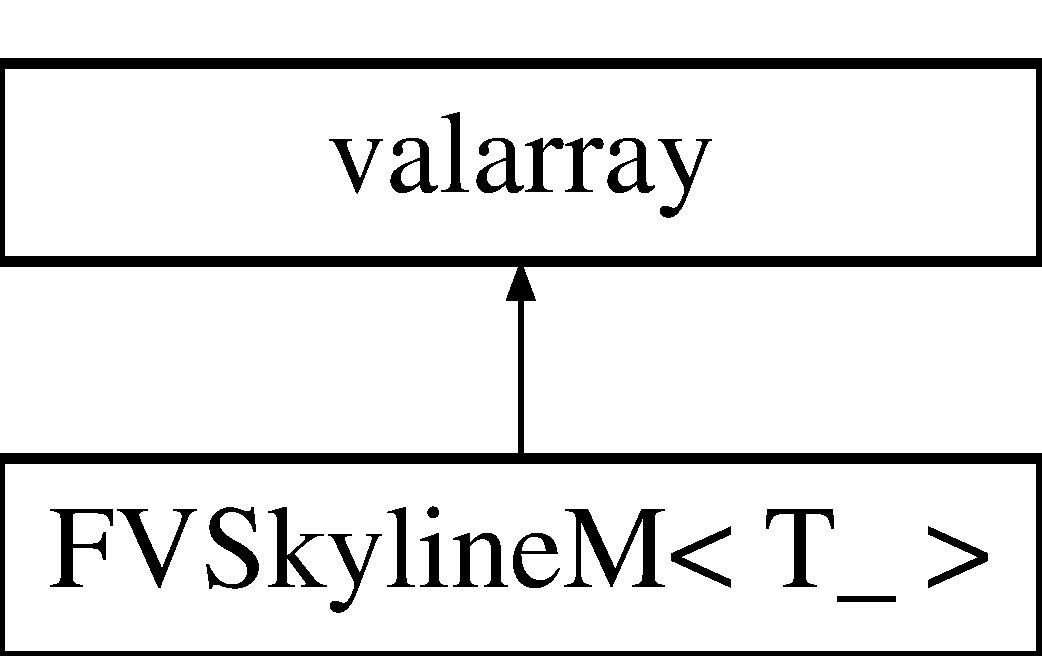
\includegraphics[height=2.000000cm]{db/d52/classvalarray}
\end{center}
\end{figure}


The documentation for this class was generated from the following file:\begin{DoxyCompactItemize}
\item 
include/\hyperlink{FVVect_8h}{FVVect.h}\end{DoxyCompactItemize}

\chapter{File Documentation}
\hypertarget{FVCell1D_8h}{
\section{include/FVCell1D.h File Reference}
\label{d9/de7/FVCell1D_8h}\index{include/FVCell1D.h@{include/FVCell1D.h}}
}
\subsection*{Data Structures}
\begin{DoxyCompactItemize}
\item 
class \hyperlink{classFVCell1D}{FVCell1D}
\end{DoxyCompactItemize}
\subsection*{Functions}
\begin{DoxyCompactItemize}
\item 
bool \hyperlink{FVCell1D_8h_af140091bdd094b2a59af97d91e7cb870}{isEqual} (\hyperlink{classFVCell1D}{FVCell1D} $\ast$c1, \hyperlink{classFVCell1D}{FVCell1D} $\ast$c2)
\end{DoxyCompactItemize}


\subsection{Function Documentation}
\hypertarget{FVCell1D_8h_af140091bdd094b2a59af97d91e7cb870}{
\index{FVCell1D.h@{FVCell1D.h}!isEqual@{isEqual}}
\index{isEqual@{isEqual}!FVCell1D.h@{FVCell1D.h}}
\subsubsection[{isEqual}]{\setlength{\rightskip}{0pt plus 5cm}bool isEqual (
\begin{DoxyParamCaption}
\item[{{\bf FVCell1D} $\ast$}]{ c1, }
\item[{{\bf FVCell1D} $\ast$}]{ c2}
\end{DoxyParamCaption}
)\hspace{0.3cm}{\ttfamily  \mbox{[}inline\mbox{]}}}}
\label{d9/de7/FVCell1D_8h_af140091bdd094b2a59af97d91e7cb870}

\hypertarget{FVCell2D_8h}{
\section{include/FVCell2D.h File Reference}
\label{d2/d6d/FVCell2D_8h}\index{include/FVCell2D.h@{include/FVCell2D.h}}
}
{\ttfamily \#include $<$vector$>$}\par
{\ttfamily \#include \char`\"{}FVPoint2D.h\char`\"{}}\par
{\ttfamily \#include \char`\"{}FVEdge2D.h\char`\"{}}\par
{\ttfamily \#include \char`\"{}FVLib\_\-config.h\char`\"{}}\par
\subsection*{Data Structures}
\begin{DoxyCompactItemize}
\item 
class \hyperlink{classFVCell2D}{FVCell2D}
\end{DoxyCompactItemize}
\subsection*{Functions}
\begin{DoxyCompactItemize}
\item 
bool \hyperlink{FVCell2D_8h_a92eb53b63fc1a120c5be43a1955b8c22}{isEqual} (\hyperlink{classFVCell2D}{FVCell2D} $\ast$c1, \hyperlink{classFVCell2D}{FVCell2D} $\ast$c2)
\end{DoxyCompactItemize}


\subsection{Function Documentation}
\hypertarget{FVCell2D_8h_a92eb53b63fc1a120c5be43a1955b8c22}{
\index{FVCell2D.h@{FVCell2D.h}!isEqual@{isEqual}}
\index{isEqual@{isEqual}!FVCell2D.h@{FVCell2D.h}}
\subsubsection[{isEqual}]{\setlength{\rightskip}{0pt plus 5cm}bool isEqual (
\begin{DoxyParamCaption}
\item[{{\bf FVCell2D} $\ast$}]{ c1, }
\item[{{\bf FVCell2D} $\ast$}]{ c2}
\end{DoxyParamCaption}
)\hspace{0.3cm}{\ttfamily  \mbox{[}inline\mbox{]}}}}
\label{d2/d6d/FVCell2D_8h_a92eb53b63fc1a120c5be43a1955b8c22}

\hypertarget{FVCell3D_8h}{
\section{include/FVCell3D.h File Reference}
\label{db/d5f/FVCell3D_8h}\index{include/FVCell3D.h@{include/FVCell3D.h}}
}
{\ttfamily \#include $<$vector$>$}\par
{\ttfamily \#include \char`\"{}FVPoint3D.h\char`\"{}}\par
{\ttfamily \#include \char`\"{}FVLib\_\-config.h\char`\"{}}\par
\subsection*{Data Structures}
\begin{DoxyCompactItemize}
\item 
class \hyperlink{classFVCell3D}{FVCell3D}
\end{DoxyCompactItemize}
\subsection*{Functions}
\begin{DoxyCompactItemize}
\item 
bool \hyperlink{FVCell3D_8h_acdd8b417e3adbfad61362bfdcc50afa0}{isEqual} (\hyperlink{classFVCell3D}{FVCell3D} $\ast$c1, \hyperlink{classFVCell3D}{FVCell3D} $\ast$c2)
\end{DoxyCompactItemize}


\subsection{Function Documentation}
\hypertarget{FVCell3D_8h_acdd8b417e3adbfad61362bfdcc50afa0}{
\index{FVCell3D.h@{FVCell3D.h}!isEqual@{isEqual}}
\index{isEqual@{isEqual}!FVCell3D.h@{FVCell3D.h}}
\subsubsection[{isEqual}]{\setlength{\rightskip}{0pt plus 5cm}bool isEqual (
\begin{DoxyParamCaption}
\item[{{\bf FVCell3D} $\ast$}]{ c1, }
\item[{{\bf FVCell3D} $\ast$}]{ c2}
\end{DoxyParamCaption}
)\hspace{0.3cm}{\ttfamily  \mbox{[}inline\mbox{]}}}}
\label{db/d5f/FVCell3D_8h_acdd8b417e3adbfad61362bfdcc50afa0}

\hypertarget{FVDenseM_8h}{
\section{include/FVDenseM.h File Reference}
\label{dc/dfc/FVDenseM_8h}\index{include/FVDenseM.h@{include/FVDenseM.h}}
}
{\ttfamily \#include \char`\"{}FVLib\_\-config.h\char`\"{}}\par
{\ttfamily \#include \char`\"{}FVGlobal.h\char`\"{}}\par
{\ttfamily \#include \char`\"{}FVVect.h\char`\"{}}\par
{\ttfamily \#include \char`\"{}FVPoint2D.h\char`\"{}}\par
{\ttfamily \#include \char`\"{}FVPoint3D.h\char`\"{}}\par
{\ttfamily \#include \char`\"{}FVPoint4D.h\char`\"{}}\par
{\ttfamily \#include $<$valarray$>$}\par
{\ttfamily \#include $<$iostream$>$}\par
{\ttfamily \#include $<$cstdio$>$}\par
{\ttfamily \#include $<$omp.h$>$}\par
{\ttfamily \#include \char`\"{}FVGlobal.h\char`\"{}}\par
\subsection*{Data Structures}
\begin{DoxyCompactItemize}
\item 
class \hyperlink{classFVDenseM}{FVDenseM$<$ T\_\- $>$}
\end{DoxyCompactItemize}
\subsection*{Functions}
\begin{DoxyCompactItemize}
\item 
{\footnotesize template$<$class T\_\- $>$ }\\\hyperlink{classFVDenseM}{FVDenseM}$<$ T\_\- $>$ \hyperlink{FVDenseM_8h_a9e3c4f4b9a12920a741a479fb9e3cbde}{operator+} (const \hyperlink{classFVDenseM}{FVDenseM}$<$ T\_\- $>$ \&aa, const \hyperlink{classFVDenseM}{FVDenseM}$<$ T\_\- $>$ \&bb)
\item 
{\footnotesize template$<$class T\_\- $>$ }\\\hyperlink{classFVDenseM}{FVDenseM}$<$ T\_\- $>$ \hyperlink{FVDenseM_8h_a182438597171752ae79fe20efb80edc2}{operator-\/} (const \hyperlink{classFVDenseM}{FVDenseM}$<$ T\_\- $>$ \&aa, const \hyperlink{classFVDenseM}{FVDenseM}$<$ T\_\- $>$ \&bb)
\item 
{\footnotesize template$<$class T\_\- $>$ }\\\hyperlink{classFVDenseM}{FVDenseM}$<$ T\_\- $>$ \hyperlink{FVDenseM_8h_aabb4419cd45c19b062e4dd90e3b6dcf6}{operator+} (const \hyperlink{classFVDenseM}{FVDenseM}$<$ T\_\- $>$ \&aa, const T\_\- \&val)
\item 
{\footnotesize template$<$class T\_\- $>$ }\\\hyperlink{classFVDenseM}{FVDenseM}$<$ T\_\- $>$ \hyperlink{FVDenseM_8h_a6bf357a19c96830c8751f9dd85b13f9b}{operator-\/} (const \hyperlink{classFVDenseM}{FVDenseM}$<$ T\_\- $>$ \&aa, const T\_\- \&val)
\item 
{\footnotesize template$<$class T\_\- $>$ }\\\hyperlink{classFVDenseM}{FVDenseM}$<$ T\_\- $>$ \hyperlink{FVDenseM_8h_ab62020d67b706f4d898b8a18de2223e3}{operator$\ast$} (const \hyperlink{classFVDenseM}{FVDenseM}$<$ T\_\- $>$ \&aa, const T\_\- \&val)
\item 
{\footnotesize template$<$class T\_\- $>$ }\\\hyperlink{classFVDenseM}{FVDenseM}$<$ T\_\- $>$ \hyperlink{FVDenseM_8h_a3b56dff6fd0bbd887964c5b412ed1127}{operator/} (const \hyperlink{classFVDenseM}{FVDenseM}$<$ T\_\- $>$ \&aa, const T\_\- \&val)
\end{DoxyCompactItemize}


\subsection{Function Documentation}
\hypertarget{FVDenseM_8h_ab62020d67b706f4d898b8a18de2223e3}{
\index{FVDenseM.h@{FVDenseM.h}!operator$\ast$@{operator$\ast$}}
\index{operator$\ast$@{operator$\ast$}!FVDenseM.h@{FVDenseM.h}}
\subsubsection[{operator$\ast$}]{\setlength{\rightskip}{0pt plus 5cm}{\bf FVDenseM}$<$T\_\-$>$ operator$\ast$ (
\begin{DoxyParamCaption}
\item[{const {\bf FVDenseM}$<$ T\_\- $>$ \&}]{ aa, }
\item[{const T\_\- \&}]{ val}
\end{DoxyParamCaption}
)}}
\label{dc/dfc/FVDenseM_8h_ab62020d67b706f4d898b8a18de2223e3}
\hypertarget{FVDenseM_8h_a9e3c4f4b9a12920a741a479fb9e3cbde}{
\index{FVDenseM.h@{FVDenseM.h}!operator+@{operator+}}
\index{operator+@{operator+}!FVDenseM.h@{FVDenseM.h}}
\subsubsection[{operator+}]{\setlength{\rightskip}{0pt plus 5cm}{\bf FVDenseM}$<$T\_\-$>$ operator+ (
\begin{DoxyParamCaption}
\item[{const {\bf FVDenseM}$<$ T\_\- $>$ \&}]{ aa, }
\item[{const {\bf FVDenseM}$<$ T\_\- $>$ \&}]{ bb}
\end{DoxyParamCaption}
)}}
\label{dc/dfc/FVDenseM_8h_a9e3c4f4b9a12920a741a479fb9e3cbde}
\hypertarget{FVDenseM_8h_aabb4419cd45c19b062e4dd90e3b6dcf6}{
\index{FVDenseM.h@{FVDenseM.h}!operator+@{operator+}}
\index{operator+@{operator+}!FVDenseM.h@{FVDenseM.h}}
\subsubsection[{operator+}]{\setlength{\rightskip}{0pt plus 5cm}{\bf FVDenseM}$<$T\_\-$>$ operator+ (
\begin{DoxyParamCaption}
\item[{const {\bf FVDenseM}$<$ T\_\- $>$ \&}]{ aa, }
\item[{const T\_\- \&}]{ val}
\end{DoxyParamCaption}
)}}
\label{dc/dfc/FVDenseM_8h_aabb4419cd45c19b062e4dd90e3b6dcf6}
\hypertarget{FVDenseM_8h_a6bf357a19c96830c8751f9dd85b13f9b}{
\index{FVDenseM.h@{FVDenseM.h}!operator-\/@{operator-\/}}
\index{operator-\/@{operator-\/}!FVDenseM.h@{FVDenseM.h}}
\subsubsection[{operator-\/}]{\setlength{\rightskip}{0pt plus 5cm}{\bf FVDenseM}$<$T\_\-$>$ operator-\/ (
\begin{DoxyParamCaption}
\item[{const {\bf FVDenseM}$<$ T\_\- $>$ \&}]{ aa, }
\item[{const T\_\- \&}]{ val}
\end{DoxyParamCaption}
)}}
\label{dc/dfc/FVDenseM_8h_a6bf357a19c96830c8751f9dd85b13f9b}
\hypertarget{FVDenseM_8h_a182438597171752ae79fe20efb80edc2}{
\index{FVDenseM.h@{FVDenseM.h}!operator-\/@{operator-\/}}
\index{operator-\/@{operator-\/}!FVDenseM.h@{FVDenseM.h}}
\subsubsection[{operator-\/}]{\setlength{\rightskip}{0pt plus 5cm}{\bf FVDenseM}$<$T\_\-$>$ operator-\/ (
\begin{DoxyParamCaption}
\item[{const {\bf FVDenseM}$<$ T\_\- $>$ \&}]{ aa, }
\item[{const {\bf FVDenseM}$<$ T\_\- $>$ \&}]{ bb}
\end{DoxyParamCaption}
)}}
\label{dc/dfc/FVDenseM_8h_a182438597171752ae79fe20efb80edc2}
\hypertarget{FVDenseM_8h_a3b56dff6fd0bbd887964c5b412ed1127}{
\index{FVDenseM.h@{FVDenseM.h}!operator/@{operator/}}
\index{operator/@{operator/}!FVDenseM.h@{FVDenseM.h}}
\subsubsection[{operator/}]{\setlength{\rightskip}{0pt plus 5cm}{\bf FVDenseM}$<$T\_\-$>$ operator/ (
\begin{DoxyParamCaption}
\item[{const {\bf FVDenseM}$<$ T\_\- $>$ \&}]{ aa, }
\item[{const T\_\- \&}]{ val}
\end{DoxyParamCaption}
)}}
\label{dc/dfc/FVDenseM_8h_a3b56dff6fd0bbd887964c5b412ed1127}

\hypertarget{FVEdge2D_8h}{
\section{include/FVEdge2D.h File Reference}
\label{d2/d44/FVEdge2D_8h}\index{include/FVEdge2D.h@{include/FVEdge2D.h}}
}
{\ttfamily \#include $<$vector$>$}\par
{\ttfamily \#include \char`\"{}FVPoint2D.h\char`\"{}}\par
{\ttfamily \#include \char`\"{}FVLib\_\-config.h\char`\"{}}\par
\subsection*{Data Structures}
\begin{DoxyCompactItemize}
\item 
class \hyperlink{classFVEdge2D}{FVEdge2D}
\end{DoxyCompactItemize}
\subsection*{Functions}
\begin{DoxyCompactItemize}
\item 
bool \hyperlink{FVEdge2D_8h_ae5709a9ce4d24448d9c1d4f955885119}{isEqual} (\hyperlink{classFVEdge2D}{FVEdge2D} $\ast$e1, \hyperlink{classFVEdge2D}{FVEdge2D} $\ast$e2)
\end{DoxyCompactItemize}


\subsection{Function Documentation}
\hypertarget{FVEdge2D_8h_ae5709a9ce4d24448d9c1d4f955885119}{
\index{FVEdge2D.h@{FVEdge2D.h}!isEqual@{isEqual}}
\index{isEqual@{isEqual}!FVEdge2D.h@{FVEdge2D.h}}
\subsubsection[{isEqual}]{\setlength{\rightskip}{0pt plus 5cm}bool isEqual (
\begin{DoxyParamCaption}
\item[{{\bf FVEdge2D} $\ast$}]{ e1, }
\item[{{\bf FVEdge2D} $\ast$}]{ e2}
\end{DoxyParamCaption}
)\hspace{0.3cm}{\ttfamily  \mbox{[}inline\mbox{]}}}}
\label{d2/d44/FVEdge2D_8h_ae5709a9ce4d24448d9c1d4f955885119}

\hypertarget{FVEdge3D_8h}{
\section{include/FVEdge3D.h File Reference}
\label{d8/d2b/FVEdge3D_8h}\index{include/FVEdge3D.h@{include/FVEdge3D.h}}
}
{\ttfamily \#include $<$vector$>$}\par
{\ttfamily \#include \char`\"{}FVPoint3D.h\char`\"{}}\par
{\ttfamily \#include \char`\"{}FVLib\_\-config.h\char`\"{}}\par
\subsection*{Data Structures}
\begin{DoxyCompactItemize}
\item 
class \hyperlink{classFVEdge3D}{FVEdge3D}
\end{DoxyCompactItemize}
\subsection*{Functions}
\begin{DoxyCompactItemize}
\item 
bool \hyperlink{FVEdge3D_8h_a433a4925600616e095ea9a95b77037e2}{isEqual} (\hyperlink{classFVEdge3D}{FVEdge3D} $\ast$e1, \hyperlink{classFVEdge3D}{FVEdge3D} $\ast$e2)
\end{DoxyCompactItemize}


\subsection{Function Documentation}
\hypertarget{FVEdge3D_8h_a433a4925600616e095ea9a95b77037e2}{
\index{FVEdge3D.h@{FVEdge3D.h}!isEqual@{isEqual}}
\index{isEqual@{isEqual}!FVEdge3D.h@{FVEdge3D.h}}
\subsubsection[{isEqual}]{\setlength{\rightskip}{0pt plus 5cm}bool isEqual (
\begin{DoxyParamCaption}
\item[{{\bf FVEdge3D} $\ast$}]{ e1, }
\item[{{\bf FVEdge3D} $\ast$}]{ e2}
\end{DoxyParamCaption}
)\hspace{0.3cm}{\ttfamily  \mbox{[}inline\mbox{]}}}}
\label{d8/d2b/FVEdge3D_8h_a433a4925600616e095ea9a95b77037e2}

\hypertarget{FVFace3D_8h}{
\section{include/FVFace3D.h File Reference}
\label{da/df7/FVFace3D_8h}\index{include/FVFace3D.h@{include/FVFace3D.h}}
}
{\ttfamily \#include $<$vector$>$}\par
{\ttfamily \#include \char`\"{}FVPoint3D.h\char`\"{}}\par
{\ttfamily \#include \char`\"{}FVLib\_\-config.h\char`\"{}}\par
\subsection*{Data Structures}
\begin{DoxyCompactItemize}
\item 
class \hyperlink{classFVFace3D}{FVFace3D}
\end{DoxyCompactItemize}
\subsection*{Functions}
\begin{DoxyCompactItemize}
\item 
bool \hyperlink{FVFace3D_8h_a004db75831951baedae791e7456c361b}{isEqual} (\hyperlink{classFVFace3D}{FVFace3D} $\ast$f1, \hyperlink{classFVFace3D}{FVFace3D} $\ast$f2)
\end{DoxyCompactItemize}


\subsection{Function Documentation}
\hypertarget{FVFace3D_8h_a004db75831951baedae791e7456c361b}{
\index{FVFace3D.h@{FVFace3D.h}!isEqual@{isEqual}}
\index{isEqual@{isEqual}!FVFace3D.h@{FVFace3D.h}}
\subsubsection[{isEqual}]{\setlength{\rightskip}{0pt plus 5cm}bool isEqual (
\begin{DoxyParamCaption}
\item[{{\bf FVFace3D} $\ast$}]{ f1, }
\item[{{\bf FVFace3D} $\ast$}]{ f2}
\end{DoxyParamCaption}
)\hspace{0.3cm}{\ttfamily  \mbox{[}inline\mbox{]}}}}
\label{da/df7/FVFace3D_8h_a004db75831951baedae791e7456c361b}

\hypertarget{FVGaussPoint_8h}{
\section{include/FVGaussPoint.h File Reference}
\label{d9/d82/FVGaussPoint_8h}\index{include/FVGaussPoint.h@{include/FVGaussPoint.h}}
}
{\ttfamily \#include \char`\"{}FVPoint2D.h\char`\"{}}\par
{\ttfamily \#include \char`\"{}FVPoint3D.h\char`\"{}}\par
{\ttfamily \#include \char`\"{}FVPoint4D.h\char`\"{}}\par
\subsection*{Data Structures}
\begin{DoxyCompactItemize}
\item 
class \hyperlink{classFVGaussPoint1D}{FVGaussPoint1D}
\item 
class \hyperlink{classFVGaussPoint2D}{FVGaussPoint2D}
\item 
class \hyperlink{classFVGaussPoint3D}{FVGaussPoint3D}
\end{DoxyCompactItemize}

\hypertarget{FVGlobal_8h}{
\section{include/FVGlobal.h File Reference}
\label{de/d64/FVGlobal_8h}\index{include/FVGlobal.h@{include/FVGlobal.h}}
}
\subsection*{Defines}
\begin{DoxyCompactItemize}
\item 
\#define \hyperlink{FVGlobal_8h_a86d500a34c624c2cae56bc25a31b12f3}{UNUSED}(\hyperlink{FVL_2FVPoint2D_8h_a9a4f74af87a76a4c3dcb729cb0e68f8d}{x})~(void)(\hyperlink{FVL_2FVPoint2D_8h_a9a4f74af87a76a4c3dcb729cb0e68f8d}{x})
\end{DoxyCompactItemize}


\subsection{Define Documentation}
\hypertarget{FVGlobal_8h_a86d500a34c624c2cae56bc25a31b12f3}{
\index{FVGlobal.h@{FVGlobal.h}!UNUSED@{UNUSED}}
\index{UNUSED@{UNUSED}!FVGlobal.h@{FVGlobal.h}}
\subsubsection[{UNUSED}]{\setlength{\rightskip}{0pt plus 5cm}\#define UNUSED(
\begin{DoxyParamCaption}
\item[{}]{{\bf x}}
\end{DoxyParamCaption}
)~(void)({\bf x})}}
\label{de/d64/FVGlobal_8h_a86d500a34c624c2cae56bc25a31b12f3}

\hypertarget{FVL_2FVGlobal_8h}{
\section{include/FVL/FVGlobal.h File Reference}
\label{de/d8f/FVL_2FVGlobal_8h}\index{include/FVL/FVGlobal.h@{include/FVL/FVGlobal.h}}
}
{\ttfamily \#include \char`\"{}FVL/FVMacros.h\char`\"{}}\par
{\ttfamily \#include \char`\"{}FVL/FVEnum.h\char`\"{}}\par

\hypertarget{FVio_8h}{
\section{include/FVio.h File Reference}
\label{d0/d8c/FVio_8h}\index{include/FVio.h@{include/FVio.h}}
}
{\ttfamily \#include $<$string$>$}\par
{\ttfamily \#include $<$iostream$>$}\par
{\ttfamily \#include $<$iomanip$>$}\par
{\ttfamily \#include $<$XML.h$>$}\par
{\ttfamily \#include $<$FVVect.h$>$}\par
{\ttfamily \#include $<$FVPoint2D.h$>$}\par
{\ttfamily \#include $<$FVPoint3D.h$>$}\par
{\ttfamily \#include $<$FVLib\_\-config.h$>$}\par
\subsection*{Data Structures}
\begin{DoxyCompactItemize}
\item 
class \hyperlink{classFVio}{FVio}
\end{DoxyCompactItemize}

\hypertarget{CFVArray_8h}{
\section{include/FVL/CFVArray.h File Reference}
\label{d6/d93/CFVArray_8h}\index{include/FVL/CFVArray.h@{include/FVL/CFVArray.h}}
}
{\ttfamily \#include $<$cuda.h$>$}\par
{\ttfamily \#include $<$cuda\_\-runtime.h$>$}\par
{\ttfamily \#include \char`\"{}FVL/FVLog.h\char`\"{}}\par
{\ttfamily \#include \char`\"{}FVL/FVArray.h\char`\"{}}\par
{\ttfamily \#include \char`\"{}FVL/templates/CFVArray.hpp\char`\"{}}\par
\subsection*{Data Structures}
\begin{DoxyCompactItemize}
\item 
class \hyperlink{classFVL_1_1CFVArray}{CFVArray$<$ T $>$}
\begin{DoxyCompactList}\small\item\em Generic CUDA-\/ready array template class. \item\end{DoxyCompactList}\end{DoxyCompactItemize}
\subsection*{Namespaces}
\begin{DoxyCompactItemize}
\item 
namespace \hyperlink{namespaceFVL}{FVL}
\end{DoxyCompactItemize}


\subsection{Detailed Description}
\begin{DoxyAuthor}{Author}
Miguel Palhas 
\end{DoxyAuthor}
\begin{DoxyDate}{Date}
13-\/02-\/2012 
\end{DoxyDate}

\hypertarget{CFVLib_8h}{
\section{include/FVL/CFVLib.h File Reference}
\label{d3/de7/CFVLib_8h}\index{include/FVL/CFVLib.h@{include/FVL/CFVLib.h}}
}
{\ttfamily \#include \char`\"{}FVL/FVGlobal.h\char`\"{}}\par
{\ttfamily \#include \char`\"{}FVL/FVLog.h\char`\"{}}\par
{\ttfamily \#include \char`\"{}FVL/FVErr.h\char`\"{}}\par
{\ttfamily \#include \char`\"{}FVL/CFVProfile.h\char`\"{}}\par
{\ttfamily \#include \char`\"{}FVL/CFVArray.h\char`\"{}}\par
{\ttfamily \#include \char`\"{}FVL/CFVPoints2D.h\char`\"{}}\par
{\ttfamily \#include \char`\"{}FVL/CFVMat.h\char`\"{}}\par
{\ttfamily \#include \char`\"{}FVL/CFVMesh2D.h\char`\"{}}\par

\hypertarget{CFVMat_8h}{
\section{include/FVL/CFVMat.h File Reference}
\label{d0/dc1/CFVMat_8h}\index{include/FVL/CFVMat.h@{include/FVL/CFVMat.h}}
}
{\ttfamily \#include $<$vector$>$}\par
{\ttfamily \#include \char`\"{}FVL/CFVArray.h\char`\"{}}\par
{\ttfamily \#include \char`\"{}FVL/templates/CFVMat.hpp\char`\"{}}\par
\subsection*{Data Structures}
\begin{DoxyCompactItemize}
\item 
class \hyperlink{classFVL_1_1CFVMat}{CFVMat$<$ T $>$}
\begin{DoxyCompactList}\small\item\em Generic CUDA-\/ready array of matrixes class. \item\end{DoxyCompactList}\end{DoxyCompactItemize}
\subsection*{Namespaces}
\begin{DoxyCompactItemize}
\item 
namespace \hyperlink{namespaceFVL}{FVL}
\end{DoxyCompactItemize}


\subsection{Detailed Description}
\begin{DoxyAuthor}{Author}
Miguel Palhas 
\end{DoxyAuthor}
\begin{DoxyDate}{Date}
13-\/02-\/2012 
\end{DoxyDate}

\hypertarget{CFVMesh2D_8h}{
\section{include/FVL/CFVMesh2D.h File Reference}
\label{db/d1b/CFVMesh2D_8h}\index{include/FVL/CFVMesh2D.h@{include/FVL/CFVMesh2D.h}}
}
{\ttfamily \#include $<$string$>$}\par
{\ttfamily \#include $<$vector$>$}\par
{\ttfamily \#include $<$cuda.h$>$}\par
{\ttfamily \#include \char`\"{}FVL/FVGlobal.h\char`\"{}}\par
{\ttfamily \#include \char`\"{}FVMesh2D.h\char`\"{}}\par
{\ttfamily \#include \char`\"{}FVL/FVLog.h\char`\"{}}\par
{\ttfamily \#include \char`\"{}FVL/CFVArray.h\char`\"{}}\par
{\ttfamily \#include \char`\"{}FVL/CFVMat.h\char`\"{}}\par
{\ttfamily \#include \char`\"{}FVL/CFVPoints2D.h\char`\"{}}\par
\subsection*{Data Structures}
\begin{DoxyCompactItemize}
\item 
struct \hyperlink{structFVL_1_1CFVMesh2D__cuda}{CFVMesh2D\_\-cuda}
\begin{DoxyCompactList}\small\item\em 2D Mesh structure to use in a CUDA device \item\end{DoxyCompactList}\item 
class \hyperlink{classFVL_1_1CFVMesh2D}{CFVMesh2D}
\begin{DoxyCompactList}\small\item\em A CUDA enabled 2D Mesh. \item\end{DoxyCompactList}\end{DoxyCompactItemize}
\subsection*{Namespaces}
\begin{DoxyCompactItemize}
\item 
namespace \hyperlink{namespaceFVL}{FVL}
\end{DoxyCompactItemize}


\subsection{Detailed Description}
\begin{DoxyAuthor}{Author}
Miguel Palhas 
\end{DoxyAuthor}
\begin{DoxyDate}{Date}
13-\/02-\/2012 
\end{DoxyDate}

\hypertarget{CFVPoints2D_8h}{
\section{include/FVL/CFVPoints2D.h File Reference}
\label{d5/da9/CFVPoints2D_8h}\index{include/FVL/CFVPoints2D.h@{include/FVL/CFVPoints2D.h}}
}
{\ttfamily \#include \char`\"{}FVL/CFVArray.h\char`\"{}}\par
\subsection*{Data Structures}
\begin{DoxyCompactItemize}
\item 
class \hyperlink{classFVL_1_1CFVPoints2D}{CFVPoints2D$<$ T $>$}
\end{DoxyCompactItemize}
\subsection*{Namespaces}
\begin{DoxyCompactItemize}
\item 
namespace \hyperlink{namespaceFVL}{FVL}
\end{DoxyCompactItemize}

\hypertarget{CFVProfile_8h}{
\section{include/FVL/CFVProfile.h File Reference}
\label{dc/d7c/CFVProfile_8h}\index{include/FVL/CFVProfile.h@{include/FVL/CFVProfile.h}}
}
{\ttfamily \#include $<$cuda.h$>$}\par
{\ttfamily \#include $<$cuda\_\-runtime.h$>$}\par
{\ttfamily \#include \char`\"{}FVL/FVGlobal.h\char`\"{}}\par
{\ttfamily \#include \char`\"{}FVL/FVLog.h\char`\"{}}\par
\subsection*{Data Structures}
\begin{DoxyCompactItemize}
\item 
class \hyperlink{classFVL_1_1CFVProfile}{CFVProfile}
\end{DoxyCompactItemize}
\subsection*{Namespaces}
\begin{DoxyCompactItemize}
\item 
namespace \hyperlink{namespaceFVL}{FVL}
\end{DoxyCompactItemize}

\hypertarget{FVArray_8h}{
\section{include/FVL/FVArray.h File Reference}
\label{d6/dbd/FVArray_8h}\index{include/FVL/FVArray.h@{include/FVL/FVArray.h}}
}
{\ttfamily \#include \char`\"{}FVL/FVLog.h\char`\"{}}\par
{\ttfamily \#include \char`\"{}FVL/templates/FVArray.hpp\char`\"{}}\par
\subsection*{Data Structures}
\begin{DoxyCompactItemize}
\item 
class \hyperlink{classFVL_1_1FVArray}{FVArray$<$ T $>$}
\begin{DoxyCompactList}\small\item\em Generic array template class. \item\end{DoxyCompactList}\end{DoxyCompactItemize}
\subsection*{Namespaces}
\begin{DoxyCompactItemize}
\item 
namespace \hyperlink{namespaceFVL}{FVL}
\end{DoxyCompactItemize}

\hypertarget{FVErr_8h}{
\section{include/FVL/FVErr.h File Reference}
\label{dc/def/FVErr_8h}\index{include/FVL/FVErr.h@{include/FVL/FVErr.h}}
}
{\ttfamily \#include $<$iostream$>$}\par
{\ttfamily \#include $<$string$>$}\par
{\ttfamily \#include $<$sstream$>$}\par
{\ttfamily \#include \char`\"{}FVL/FVLog.h\char`\"{}}\par
\subsection*{Data Structures}
\begin{DoxyCompactItemize}
\item 
class \hyperlink{classFVL_1_1FVErr}{FVErr}
\end{DoxyCompactItemize}
\subsection*{Namespaces}
\begin{DoxyCompactItemize}
\item 
namespace \hyperlink{namespaceFVL}{FVL}
\end{DoxyCompactItemize}

\hypertarget{FVL_2FVLib_8h}{
\section{include/FVL/FVLib.h File Reference}
\label{d1/d68/FVL_2FVLib_8h}\index{include/FVL/FVLib.h@{include/FVL/FVLib.h}}
}
{\ttfamily \#include \char`\"{}FVL/FVMacros.h\char`\"{}}\par
{\ttfamily \#include \char`\"{}FVL/FVEnum.h\char`\"{}}\par
{\ttfamily \#include \char`\"{}FVL/CFVPoints2D.h\char`\"{}}\par
{\ttfamily \#include \char`\"{}FVL/CFVMesh2D.h\char`\"{}}\par
{\ttfamily \#include \char`\"{}FVL/FVErr.h\char`\"{}}\par
{\ttfamily \#include \char`\"{}FVL/FVLog.h\char`\"{}}\par
{\ttfamily \#include \char`\"{}FVL/FVXMLReader.h\char`\"{}}\par
{\ttfamily \#include \char`\"{}FVL/FVXMLWriter.h\char`\"{}}\par
{\ttfamily \#include \char`\"{}FVL/CFVLib.h\char`\"{}}\par

\hypertarget{FVLib_8h}{
\section{include/FVLib.h File Reference}
\label{d3/ddf/FVLib_8h}\index{include/FVLib.h@{include/FVLib.h}}
}
{\ttfamily \#include \char`\"{}FVGlobal.h\char`\"{}}\par
{\ttfamily \#include \char`\"{}FVLib\_\-config.h\char`\"{}}\par
{\ttfamily \#include \char`\"{}FVMesh1D.h\char`\"{}}\par
{\ttfamily \#include \char`\"{}FVMesh2D.h\char`\"{}}\par
{\ttfamily \#include \char`\"{}FVMesh3D.h\char`\"{}}\par
{\ttfamily \#include \char`\"{}Gmsh.h\char`\"{}}\par
{\ttfamily \#include \char`\"{}Parameter.h\char`\"{}}\par
{\ttfamily \#include \char`\"{}Table.h\char`\"{}}\par
{\ttfamily \#include \char`\"{}FVVect.h\char`\"{}}\par
{\ttfamily \#include \char`\"{}FVDenseM.h\char`\"{}}\par
{\ttfamily \#include \char`\"{}FVSparseM.h\char`\"{}}\par
{\ttfamily \#include \char`\"{}FVGaussPoint.h\char`\"{}}\par
{\ttfamily \#include \char`\"{}FVStencil.h\char`\"{}}\par
{\ttfamily \#include \char`\"{}FVRecons1D.h\char`\"{}}\par
{\ttfamily \#include \char`\"{}FVRecons2D.h\char`\"{}}\par
{\ttfamily \#include \char`\"{}FVRecons3D.h\char`\"{}}\par

\hypertarget{FVLog_8h}{
\section{include/FVL/FVLog.h File Reference}
\label{db/dc6/FVLog_8h}\index{include/FVL/FVLog.h@{include/FVL/FVLog.h}}
}
{\ttfamily \#include $<$ctime$>$}\par
{\ttfamily \#include $<$string$>$}\par
{\ttfamily \#include $<$fstream$>$}\par
{\ttfamily \#include \char`\"{}FVL/FVGlobal.h\char`\"{}}\par
\subsection*{Data Structures}
\begin{DoxyCompactItemize}
\item 
class \hyperlink{classFVL_1_1FVLog}{FVLog}
\end{DoxyCompactItemize}
\subsection*{Namespaces}
\begin{DoxyCompactItemize}
\item 
namespace \hyperlink{namespaceFVL}{FVL}
\end{DoxyCompactItemize}

\hypertarget{FVParameter_8h}{
\section{include/FVL/FVParameter.h File Reference}
\label{d9/d10/FVParameter_8h}\index{include/FVL/FVParameter.h@{include/FVL/FVParameter.h}}
}

\hypertarget{FVL_2FVPoint2D_8h}{
\section{include/FVL/FVPoint2D.h File Reference}
\label{d7/d79/FVL_2FVPoint2D_8h}\index{include/FVL/FVPoint2D.h@{include/FVL/FVPoint2D.h}}
}
{\ttfamily \#include $<$cmath$>$}\par
{\ttfamily \#include $<$iostream$>$}\par
{\ttfamily \#include $<$iomanip$>$}\par
{\ttfamily \#include \char`\"{}FVL/FVGlobal.h\char`\"{}}\par
\subsection*{Data Structures}
\begin{DoxyCompactItemize}
\item 
class \hyperlink{classFVL_1_1FVPoint2D}{FVPoint2D$<$ T $>$}
\end{DoxyCompactItemize}
\subsection*{Namespaces}
\begin{DoxyCompactItemize}
\item 
namespace \hyperlink{namespaceFVL}{FVL}
\end{DoxyCompactItemize}
\subsection*{Functions}
\begin{DoxyCompactItemize}
\item 
{\footnotesize template$<$class T $>$ }\\class \hyperlink{classFVL_1_1FVPoint2D}{FVL::FVPoint2D} \hyperlink{namespaceFVL_a9d63c61da787909700ebd6753c6c8b4d}{operator} (const \hyperlink{classFVPoint2D}{FVPoint2D}$<$ T $>$ \&a, const \hyperlink{classFVPoint2D}{FVPoint2D}$<$ T $>$ \&b)
\item 
\hyperlink{FVL_2FVPoint2D_8h_ae4279cd9e822c40257d07ae337bccc81}{FVPoint2D} ()
\item 
\hyperlink{FVL_2FVPoint2D_8h_a6e6f7177e1ca2b77b8bc2e965be6009f}{FVPoint2D} (T new\_\-x, T new\_\-y)
\item 
\hyperlink{FVL_2FVPoint2D_8h_a092586f141802d534434f1bd00ae8fc0}{FVPoint2D} (const FVPoint$<$ T $>$ \&copy)
\item 
\hyperlink{classFVPoint2D}{FVPoint2D}$<$ T $>$ \& \hyperlink{FVL_2FVPoint2D_8h_a6506f9b86ca79cb020844043fcfaee87}{operator+=} (const \hyperlink{classFVPoint2D}{FVPoint2D}$<$ T $>$ \&p)
\item 
\hyperlink{classFVPoint2D}{FVPoint2D}$<$ T $>$ \& \hyperlink{FVL_2FVPoint2D_8h_afb28d20e69c207f3a5c5c410483c98a7}{operator-\/=} (const \hyperlink{classFVPoint2D}{FVPoint2D}$<$ T $>$ \&p)
\item 
\hyperlink{classFVPoint2D}{FVPoint2D}$<$ T $>$ \& \hyperlink{FVL_2FVPoint2D_8h_a9ee5dfd004992388e4bde8dae4322608}{operator=} (const T \&a)
\item 
\hyperlink{classFVPoint2D}{FVPoint2D}$<$ T $>$ \& \hyperlink{FVL_2FVPoint2D_8h_ad2dcd7ad2b05fefa71c217248a6d9692}{operator+=} (const T \&a)
\item 
\hyperlink{classFVPoint2D}{FVPoint2D}$<$ T $>$ \& \hyperlink{FVL_2FVPoint2D_8h_a39b95fb0cd805b762fd538fa50403b6c}{operator-\/=} (const T \&a)
\item 
\hyperlink{classFVPoint2D}{FVPoint2D}$<$ T $>$ \& \hyperlink{FVL_2FVPoint2D_8h_a1d61410c16c6eea601ea750317bd558d}{operator$\ast$=} (const T \&a)
\item 
\hyperlink{classFVPoint2D}{FVPoint2D}$<$ T $>$ \& \hyperlink{FVL_2FVPoint2D_8h_adc89028b210045c3f8af0975aabea77e}{operator/=} (const T \&a)
\item 
T \hyperlink{FVL_2FVPoint2D_8h_a9923476b2d9dfbf7187a40f1d58251b5}{determinant} (const \hyperlink{classFVPoint2D}{FVPoint2D}$<$ T $>$ \&b)
\item 
T \hyperlink{FVL_2FVPoint2D_8h_a2c355d93f615826f8d1715dcca908cf8}{norm} ()
\item 
{\footnotesize template$<$class T $>$ }\\\hyperlink{classFVPoint2D}{FVPoint2D}$<$ T $>$ \hyperlink{namespaceFVL_a7d5cb24f219876bf12dc09b7bf61aced}{operator-\/} (const \hyperlink{classFVPoint2D}{FVPoint2D}$<$ T $>$ \&a, const \hyperlink{classFVPoint2D}{FVPoint2D}$<$ T $>$ \&b)
\item 
{\footnotesize template$<$class T $>$ }\\\hyperlink{classFVPoint2D}{FVPoint2D}$<$ T $>$ \hyperlink{namespaceFVL_adbed70591d9eda691e7b13d65522442a}{operator$\ast$} (const \hyperlink{classFVPoint2D}{FVPoint2D}$<$ T $>$ \&a, const \hyperlink{classFVPoint2D}{FVPoint2D}$<$ T $>$ \&b)
\item 
{\footnotesize template$<$class T $>$ }\\\hyperlink{classFVPoint2D}{FVPoint2D}$<$ T $>$ \hyperlink{namespaceFVL_a2744005a9d13a03dbd598b60efb9e886}{operator/} (const \hyperlink{classFVPoint2D}{FVPoint2D}$<$ T $>$ \&a, const \hyperlink{classFVPoint2D}{FVPoint2D}$<$ T $>$ \&b)
\item 
{\footnotesize template$<$class T $>$ }\\\hyperlink{classFVPoint2D}{FVPoint2D}$<$ T $>$ \hyperlink{namespaceFVL_ac45bd75690254ff12861d49e8f099eef}{operator+} (const \hyperlink{classFVPoint2D}{FVPoint2D}$<$ T $>$ \&a, const T \&\hyperlink{FVL_2FVPoint2D_8h_a9a4f74af87a76a4c3dcb729cb0e68f8d}{x})
\item 
{\footnotesize template$<$class T $>$ }\\\hyperlink{classFVPoint2D}{FVPoint2D}$<$ T $>$ \hyperlink{namespaceFVL_a790238a5d379903700a9ca768581f476}{operator-\/} (const \hyperlink{classFVPoint2D}{FVPoint2D}$<$ T $>$ \&a, const T \&\hyperlink{FVL_2FVPoint2D_8h_a9a4f74af87a76a4c3dcb729cb0e68f8d}{x})
\item 
{\footnotesize template$<$class T $>$ }\\\hyperlink{classFVPoint2D}{FVPoint2D}$<$ T $>$ \hyperlink{namespaceFVL_a9182bd9a6593151a580c126b2b9a95a7}{operator$\ast$} (const \hyperlink{classFVPoint2D}{FVPoint2D}$<$ T $>$ \&a, const T \&\hyperlink{FVL_2FVPoint2D_8h_a9a4f74af87a76a4c3dcb729cb0e68f8d}{x})
\item 
{\footnotesize template$<$class T $>$ }\\\hyperlink{classFVPoint2D}{FVPoint2D}$<$ T $>$ \hyperlink{namespaceFVL_a2c00ee27a6efec77777d871f17c4a8ad}{operator$\ast$} (const T \&\hyperlink{FVL_2FVPoint2D_8h_a9a4f74af87a76a4c3dcb729cb0e68f8d}{x}, const FVpoint2D$<$ T $>$ \&a)
\item 
{\footnotesize template$<$class T $>$ }\\\hyperlink{classFVPoint2D}{FVPoint2D}$<$ T $>$ \hyperlink{namespaceFVL_a101d709be4cbb8fbf4d3d6dea90b2e89}{operator/} (const \hyperlink{classFVPoint2D}{FVPoint2D}$<$ T $>$ \&a, const T \&\hyperlink{FVL_2FVPoint2D_8h_a9a4f74af87a76a4c3dcb729cb0e68f8d}{x})
\item 
{\footnotesize template$<$class T $>$ }\\\hyperlink{classFVPoint2D}{FVPoint2D}$<$ T $>$ \hyperlink{namespaceFVL_af2e46d2e39647630b0c1cc146298ef33}{operator-\/} (const \hyperlink{classFVPoint2D}{FVPoint2D}$<$ T $>$ \&a)
\item 
{\footnotesize template$<$class T $>$ }\\std::ostream \& \hyperlink{namespaceFVL_a2c42a06efa3c35dd1fc72c25430a1b1c}{operator$<$$<$} (std::ostream \&s, const \hyperlink{classFVPoint2D}{FVPoint2D}$<$ T $>$ \&p)
\end{DoxyCompactItemize}
\subsection*{Variables}
\begin{DoxyCompactItemize}
\item 
T \hyperlink{FVL_2FVPoint2D_8h_a9a4f74af87a76a4c3dcb729cb0e68f8d}{x}
\item 
T \hyperlink{FVL_2FVPoint2D_8h_a1cb2b5ea04251d543e49356ef54eb853}{y}
\end{DoxyCompactItemize}


\subsection{Function Documentation}
\hypertarget{FVL_2FVPoint2D_8h_a9923476b2d9dfbf7187a40f1d58251b5}{
\index{FVL/FVPoint2D.h@{FVL/FVPoint2D.h}!determinant@{determinant}}
\index{determinant@{determinant}!FVL/FVPoint2D.h@{FVL/FVPoint2D.h}}
\subsubsection[{determinant}]{\setlength{\rightskip}{0pt plus 5cm}T operator::determinant (
\begin{DoxyParamCaption}
\item[{const {\bf FVPoint2D}$<$ T $>$ \&}]{ b}
\end{DoxyParamCaption}
)\hspace{0.3cm}{\ttfamily  \mbox{[}inline\mbox{]}}}}
\label{d7/d79/FVL_2FVPoint2D_8h_a9923476b2d9dfbf7187a40f1d58251b5}
\hypertarget{FVL_2FVPoint2D_8h_a092586f141802d534434f1bd00ae8fc0}{
\index{FVL/FVPoint2D.h@{FVL/FVPoint2D.h}!FVPoint2D@{FVPoint2D}}
\index{FVPoint2D@{FVPoint2D}!FVL/FVPoint2D.h@{FVL/FVPoint2D.h}}
\subsubsection[{FVPoint2D}]{\setlength{\rightskip}{0pt plus 5cm}operator::FVPoint2D (
\begin{DoxyParamCaption}
\item[{const FVPoint$<$ T $>$ \&}]{ copy}
\end{DoxyParamCaption}
)}}
\label{d7/d79/FVL_2FVPoint2D_8h_a092586f141802d534434f1bd00ae8fc0}
\hypertarget{FVL_2FVPoint2D_8h_ae4279cd9e822c40257d07ae337bccc81}{
\index{FVL/FVPoint2D.h@{FVL/FVPoint2D.h}!FVPoint2D@{FVPoint2D}}
\index{FVPoint2D@{FVPoint2D}!FVL/FVPoint2D.h@{FVL/FVPoint2D.h}}
\subsubsection[{FVPoint2D}]{\setlength{\rightskip}{0pt plus 5cm}operator::FVPoint2D (
\begin{DoxyParamCaption}
{}
\end{DoxyParamCaption}
)}}
\label{d7/d79/FVL_2FVPoint2D_8h_ae4279cd9e822c40257d07ae337bccc81}
\hypertarget{FVL_2FVPoint2D_8h_a6e6f7177e1ca2b77b8bc2e965be6009f}{
\index{FVL/FVPoint2D.h@{FVL/FVPoint2D.h}!FVPoint2D@{FVPoint2D}}
\index{FVPoint2D@{FVPoint2D}!FVL/FVPoint2D.h@{FVL/FVPoint2D.h}}
\subsubsection[{FVPoint2D}]{\setlength{\rightskip}{0pt plus 5cm}operator::FVPoint2D (
\begin{DoxyParamCaption}
\item[{T}]{ new\_\-x, }
\item[{T}]{ new\_\-y}
\end{DoxyParamCaption}
)}}
\label{d7/d79/FVL_2FVPoint2D_8h_a6e6f7177e1ca2b77b8bc2e965be6009f}
\hypertarget{FVL_2FVPoint2D_8h_a2c355d93f615826f8d1715dcca908cf8}{
\index{FVL/FVPoint2D.h@{FVL/FVPoint2D.h}!norm@{norm}}
\index{norm@{norm}!FVL/FVPoint2D.h@{FVL/FVPoint2D.h}}
\subsubsection[{norm}]{\setlength{\rightskip}{0pt plus 5cm}T operator::norm (
\begin{DoxyParamCaption}
{}
\end{DoxyParamCaption}
)\hspace{0.3cm}{\ttfamily  \mbox{[}inline\mbox{]}}}}
\label{d7/d79/FVL_2FVPoint2D_8h_a2c355d93f615826f8d1715dcca908cf8}
\hypertarget{FVL_2FVPoint2D_8h_a1d61410c16c6eea601ea750317bd558d}{
\index{FVL/FVPoint2D.h@{FVL/FVPoint2D.h}!operator$\ast$=@{operator$\ast$=}}
\index{operator$\ast$=@{operator$\ast$=}!FVL/FVPoint2D.h@{FVL/FVPoint2D.h}}
\subsubsection[{operator$\ast$=}]{\setlength{\rightskip}{0pt plus 5cm}{\bf FVPoint2D}$<$T$>$\& operator::operator$\ast$= (
\begin{DoxyParamCaption}
\item[{const T \&}]{ a}
\end{DoxyParamCaption}
)}}
\label{d7/d79/FVL_2FVPoint2D_8h_a1d61410c16c6eea601ea750317bd558d}
\hypertarget{FVL_2FVPoint2D_8h_ad2dcd7ad2b05fefa71c217248a6d9692}{
\index{FVL/FVPoint2D.h@{FVL/FVPoint2D.h}!operator+=@{operator+=}}
\index{operator+=@{operator+=}!FVL/FVPoint2D.h@{FVL/FVPoint2D.h}}
\subsubsection[{operator+=}]{\setlength{\rightskip}{0pt plus 5cm}{\bf FVPoint2D}$<$T$>$\& operator::operator+= (
\begin{DoxyParamCaption}
\item[{const T \&}]{ a}
\end{DoxyParamCaption}
)}}
\label{d7/d79/FVL_2FVPoint2D_8h_ad2dcd7ad2b05fefa71c217248a6d9692}
\hypertarget{FVL_2FVPoint2D_8h_a6506f9b86ca79cb020844043fcfaee87}{
\index{FVL/FVPoint2D.h@{FVL/FVPoint2D.h}!operator+=@{operator+=}}
\index{operator+=@{operator+=}!FVL/FVPoint2D.h@{FVL/FVPoint2D.h}}
\subsubsection[{operator+=}]{\setlength{\rightskip}{0pt plus 5cm}{\bf FVPoint2D}$<$T$>$\& operator::operator+= (
\begin{DoxyParamCaption}
\item[{const {\bf FVPoint2D}$<$ T $>$ \&}]{ p}
\end{DoxyParamCaption}
)}}
\label{d7/d79/FVL_2FVPoint2D_8h_a6506f9b86ca79cb020844043fcfaee87}
\hypertarget{FVL_2FVPoint2D_8h_a39b95fb0cd805b762fd538fa50403b6c}{
\index{FVL/FVPoint2D.h@{FVL/FVPoint2D.h}!operator-\/=@{operator-\/=}}
\index{operator-\/=@{operator-\/=}!FVL/FVPoint2D.h@{FVL/FVPoint2D.h}}
\subsubsection[{operator-\/=}]{\setlength{\rightskip}{0pt plus 5cm}{\bf FVPoint2D}$<$T$>$\& operator::operator-\/= (
\begin{DoxyParamCaption}
\item[{const T \&}]{ a}
\end{DoxyParamCaption}
)}}
\label{d7/d79/FVL_2FVPoint2D_8h_a39b95fb0cd805b762fd538fa50403b6c}
\hypertarget{FVL_2FVPoint2D_8h_afb28d20e69c207f3a5c5c410483c98a7}{
\index{FVL/FVPoint2D.h@{FVL/FVPoint2D.h}!operator-\/=@{operator-\/=}}
\index{operator-\/=@{operator-\/=}!FVL/FVPoint2D.h@{FVL/FVPoint2D.h}}
\subsubsection[{operator-\/=}]{\setlength{\rightskip}{0pt plus 5cm}{\bf FVPoint2D}$<$T$>$\& operator::operator-\/= (
\begin{DoxyParamCaption}
\item[{const {\bf FVPoint2D}$<$ T $>$ \&}]{ p}
\end{DoxyParamCaption}
)}}
\label{d7/d79/FVL_2FVPoint2D_8h_afb28d20e69c207f3a5c5c410483c98a7}
\hypertarget{FVL_2FVPoint2D_8h_adc89028b210045c3f8af0975aabea77e}{
\index{FVL/FVPoint2D.h@{FVL/FVPoint2D.h}!operator/=@{operator/=}}
\index{operator/=@{operator/=}!FVL/FVPoint2D.h@{FVL/FVPoint2D.h}}
\subsubsection[{operator/=}]{\setlength{\rightskip}{0pt plus 5cm}{\bf FVPoint2D}$<$T$>$\& operator::operator/= (
\begin{DoxyParamCaption}
\item[{const T \&}]{ a}
\end{DoxyParamCaption}
)}}
\label{d7/d79/FVL_2FVPoint2D_8h_adc89028b210045c3f8af0975aabea77e}
\hypertarget{FVL_2FVPoint2D_8h_a9ee5dfd004992388e4bde8dae4322608}{
\index{FVL/FVPoint2D.h@{FVL/FVPoint2D.h}!operator=@{operator=}}
\index{operator=@{operator=}!FVL/FVPoint2D.h@{FVL/FVPoint2D.h}}
\subsubsection[{operator=}]{\setlength{\rightskip}{0pt plus 5cm}{\bf FVPoint2D}$<$T$>$\& operator::operator= (
\begin{DoxyParamCaption}
\item[{const T \&}]{ a}
\end{DoxyParamCaption}
)}}
\label{d7/d79/FVL_2FVPoint2D_8h_a9ee5dfd004992388e4bde8dae4322608}


\subsection{Variable Documentation}
\hypertarget{FVL_2FVPoint2D_8h_a9a4f74af87a76a4c3dcb729cb0e68f8d}{
\index{FVL/FVPoint2D.h@{FVL/FVPoint2D.h}!x@{x}}
\index{x@{x}!FVL/FVPoint2D.h@{FVL/FVPoint2D.h}}
\subsubsection[{x}]{\setlength{\rightskip}{0pt plus 5cm}T {\bf x}}}
\label{d7/d79/FVL_2FVPoint2D_8h_a9a4f74af87a76a4c3dcb729cb0e68f8d}
\hypertarget{FVL_2FVPoint2D_8h_a1cb2b5ea04251d543e49356ef54eb853}{
\index{FVL/FVPoint2D.h@{FVL/FVPoint2D.h}!y@{y}}
\index{y@{y}!FVL/FVPoint2D.h@{FVL/FVPoint2D.h}}
\subsubsection[{y}]{\setlength{\rightskip}{0pt plus 5cm}T {\bf y}}}
\label{d7/d79/FVL_2FVPoint2D_8h_a1cb2b5ea04251d543e49356ef54eb853}

\hypertarget{FVPoint2D_8h}{
\section{include/FVL/FVPoint2D.h File Reference}
\label{d8/d53/FVPoint2D_8h}\index{include/FVL/FVPoint2D.h@{include/FVL/FVPoint2D.h}}
}
{\ttfamily \#include $<$cmath$>$}\par
{\ttfamily \#include $<$iostream$>$}\par
{\ttfamily \#include $<$iomanip$>$}\par
{\ttfamily \#include \char`\"{}FVL/FVGlobal.h\char`\"{}}\par
\subsection*{Data Structures}
\begin{DoxyCompactItemize}
\item 
class \hyperlink{classFVL_1_1FVPoint2D}{FVPoint2D$<$ T $>$}
\end{DoxyCompactItemize}
\subsection*{Namespaces}
\begin{DoxyCompactItemize}
\item 
namespace \hyperlink{namespaceFVL}{FVL}
\end{DoxyCompactItemize}

\hypertarget{FVXMLReader_8h}{
\section{include/FVL/FVXMLReader.h File Reference}
\label{d8/d1a/FVXMLReader_8h}\index{include/FVL/FVXMLReader.h@{include/FVL/FVXMLReader.h}}
}
{\ttfamily \#include $<$vector$>$}\par
{\ttfamily \#include $<$sstream$>$}\par
{\ttfamily \#include $<$string$>$}\par
{\ttfamily \#include \char`\"{}rapidxml/rapidxml.hpp\char`\"{}}\par
{\ttfamily \#include \char`\"{}FVL/CFVArray.h\char`\"{}}\par
{\ttfamily \#include \char`\"{}FVL/CFVPoints2D.h\char`\"{}}\par
{\ttfamily \#include \char`\"{}FVL/templates/FVXMLReader.hpp\char`\"{}}\par
\subsection*{Data Structures}
\begin{DoxyCompactItemize}
\item 
class \hyperlink{classFVL_1_1FVXMLReader}{FVXMLReader}
\end{DoxyCompactItemize}
\subsection*{Namespaces}
\begin{DoxyCompactItemize}
\item 
namespace \hyperlink{namespaceFVL}{FVL}
\end{DoxyCompactItemize}
\subsection*{Variables}
\begin{DoxyCompactItemize}
\item 
\hyperlink{classFVL_1_1FVXMLReader}{FVL::FVXMLReader} \hyperlink{namespaceFVL_aa44c792c5d125745a60768dc48554744}{operator}
\end{DoxyCompactItemize}

\hypertarget{FVXMLWriter_8h}{
\section{include/FVL/FVXMLWriter.h File Reference}
\label{d9/d7f/FVXMLWriter_8h}\index{include/FVL/FVXMLWriter.h@{include/FVL/FVXMLWriter.h}}
}
{\ttfamily \#include $<$sstream$>$}\par
{\ttfamily \#include $<$iomanip$>$}\par
{\ttfamily \#include $<$iostream$>$}\par
{\ttfamily \#include $<$fstream$>$}\par
{\ttfamily \#include $<$string$>$}\par
{\ttfamily \#include $<$vector$>$}\par
{\ttfamily \#include \char`\"{}FVL/CFVArray.h\char`\"{}}\par
{\ttfamily \#include \char`\"{}rapidxml/rapidxml.hpp\char`\"{}}\par
{\ttfamily \#include \char`\"{}rapidxml/rapidxml\_\-print.hpp\char`\"{}}\par
{\ttfamily \#include \char`\"{}FVL/templates/FVXMLWriter.hpp\char`\"{}}\par
\subsection*{Data Structures}
\begin{DoxyCompactItemize}
\item 
class \hyperlink{classFVL_1_1FVXMLWriter}{FVXMLWriter}
\end{DoxyCompactItemize}
\subsection*{Namespaces}
\begin{DoxyCompactItemize}
\item 
namespace \hyperlink{namespaceFVL}{FVL}
\end{DoxyCompactItemize}

\hypertarget{CFVArray_8hpp}{
\section{include/FVL/templates/CFVArray.hpp File Reference}
\label{dd/d00/CFVArray_8hpp}\index{include/FVL/templates/CFVArray.hpp@{include/FVL/templates/CFVArray.hpp}}
}


\subsection{Detailed Description}
\begin{DoxyAuthor}{Author}
Miguel Palhas 
\end{DoxyAuthor}
\begin{DoxyDate}{Date}
13-\/02-\/2012 
\end{DoxyDate}

\hypertarget{CFVMat_8hpp}{
\section{include/FVL/templates/CFVMat.hpp File Reference}
\label{d5/d84/CFVMat_8hpp}\index{include/FVL/templates/CFVMat.hpp@{include/FVL/templates/CFVMat.hpp}}
}

\hypertarget{FVArray_8hpp}{
\section{include/FVL/templates/FVArray.hpp File Reference}
\label{de/da8/FVArray_8hpp}\index{include/FVL/templates/FVArray.hpp@{include/FVL/templates/FVArray.hpp}}
}

\hypertarget{FVXMLReader_8hpp}{
\section{include/FVL/templates/FVXMLReader.hpp File Reference}
\label{d8/df6/FVXMLReader_8hpp}\index{include/FVL/templates/FVXMLReader.hpp@{include/FVL/templates/FVXMLReader.hpp}}
}

\hypertarget{FVXMLWriter_8hpp}{
\section{include/FVL/templates/FVXMLWriter.hpp File Reference}
\label{d2/d38/FVXMLWriter_8hpp}\index{include/FVL/templates/FVXMLWriter.hpp@{include/FVL/templates/FVXMLWriter.hpp}}
}

\hypertarget{FVLib__config_8h}{
\section{include/FVLib\_\-config.h File Reference}
\label{d0/d7e/FVLib__config_8h}\index{include/FVLib\_\-config.h@{include/FVLib\_\-config.h}}
}
{\ttfamily \#include $<$string$>$}\par
{\ttfamily \#include $<$map$>$}\par
\subsection*{Defines}
\begin{DoxyCompactItemize}
\item 
\#define \hyperlink{FVLib__config_8h_a0aecb3ad18ff59ff7d55a00aa937a169}{INF\_\-MIN}~(-\/1.E+100)
\item 
\#define \hyperlink{FVLib__config_8h_a46c621c59d887261122f6e38fb055af4}{SUP\_\-MAX}~(1.E+100)
\item 
\#define \hyperlink{FVLib__config_8h_a3ec8923fbea44f77ad7349392edce89c}{FVDOUBLE\_\-PRECISION}~1.E-\/17
\item 
\#define \hyperlink{FVLib__config_8h_a4c8b993873b1a6eb67bdf2e259457b64}{FVPRECISION}~12
\item 
\#define \hyperlink{FVLib__config_8h_a77ebba00bc4f746080c4abbbec6954f0}{FVCHAMP}~20
\item 
\#define \hyperlink{FVLib__config_8h_a02cc6ca8a396bcf8b2c2d701a8c19209}{FVCHAMPINT}~10
\item 
\#define \hyperlink{FVLib__config_8h_ae9c36a36eec849a351732799796171a4}{NB\_\-CELL\_\-PER\_\-VERTEX\_\-2D}~12
\item 
\#define \hyperlink{FVLib__config_8h_a3e6d61c39df01604f75ed52fa5cd4d86}{NB\_\-VERTEX\_\-PER\_\-CELL\_\-2D}~9
\item 
\#define \hyperlink{FVLib__config_8h_ad8f3930b0e6660a990afd5ee6b865679}{NB\_\-EDGE\_\-PER\_\-CELL\_\-2D}~9
\item 
\#define \hyperlink{FVLib__config_8h_a5fd3862d0076515b1faecf6989d99faa}{NB\_\-CELL\_\-PER\_\-VERTEX\_\-3D}~60
\item 
\#define \hyperlink{FVLib__config_8h_afa47eea7fa7d5b622c2dc672bf147a6f}{NB\_\-VERTEX\_\-PER\_\-FACE\_\-3D}~9
\item 
\#define \hyperlink{FVLib__config_8h_a0ea2b692734b03edc350f6d0b3f47b41}{NB\_\-EDGE\_\-PER\_\-FACE\_\-3D}~9
\item 
\#define \hyperlink{FVLib__config_8h_a8e4243abcafd0ad62d9c49c8e6eac3bb}{NB\_\-VERTEX\_\-PER\_\-CELL\_\-3D}~9
\item 
\#define \hyperlink{FVLib__config_8h_a025b20104f64ef9d963e9291e9285235}{NB\_\-FACE\_\-PER\_\-CELL\_\-3D}~9
\item 
\#define \hyperlink{FVLib__config_8h_a22edb4c48e284ad253bca6e114dc7b1e}{GMSH\_\-NB\_\-NODE\_\-PER\_\-ELEMENT}~9
\item 
\#define \hyperlink{FVLib__config_8h_a69a7e49cc9c390652f228f7a334e12aa}{MINUS\_\-THREE\_\-DIM}~2147483648
\item 
\#define \hyperlink{FVLib__config_8h_ac071f5c6770b46e8ed7203cbee3548a6}{MINUS\_\-TWO\_\-DIM}~1073741824
\item 
\#define \hyperlink{FVLib__config_8h_ae6bc19d29d02917671caed83601ecbf7}{MINUS\_\-ONE\_\-DIM}~536870912
\end{DoxyCompactItemize}
\subsection*{Typedefs}
\begin{DoxyCompactItemize}
\item 
typedef std::map$<$ std::string, std::string $>$ \hyperlink{FVLib__config_8h_a09af799878f7f9f2af8b7133bc151874}{StringMap}
\end{DoxyCompactItemize}
\subsection*{Enumerations}
\begin{DoxyCompactItemize}
\item 
enum \hyperlink{FVLib__config_8h_a5cf6a56f5e7b6ab58f37c0ca37668970}{FVFile} \{ \par
\hyperlink{FVLib__config_8h_a5cf6a56f5e7b6ab58f37c0ca37668970a9922fa78474d80301a2bd53dbef40f77}{FVNULL} =  0, 
\hyperlink{FVLib__config_8h_a5cf6a56f5e7b6ab58f37c0ca37668970a938aeebef6396dc7df1ea384074e0c6d}{FVOK}, 
\hyperlink{FVLib__config_8h_a5cf6a56f5e7b6ab58f37c0ca37668970a1672402149583c19aa4d056cf35ccf06}{FVREAD}, 
\hyperlink{FVLib__config_8h_a5cf6a56f5e7b6ab58f37c0ca37668970ac558ceda6d9ad208b2b3c02e8a9c0f6f}{FVWRITE}, 
\par
\hyperlink{FVLib__config_8h_a5cf6a56f5e7b6ab58f37c0ca37668970a4ecfc4552305899b3f0c6b1ad8708b8a}{FVENDFILE}, 
\hyperlink{FVLib__config_8h_a5cf6a56f5e7b6ab58f37c0ca37668970a06b9e1a5b179f11a410737dfe46cc049}{FVNOFILE}, 
\hyperlink{FVLib__config_8h_a5cf6a56f5e7b6ab58f37c0ca37668970a4f2503f7967079a97ae18320ee0f3c38}{FVWRONGDIM}, 
\hyperlink{FVLib__config_8h_a5cf6a56f5e7b6ab58f37c0ca37668970adbeaf9eb86081d5526f641854900e280}{FVERROR}, 
\par
\hyperlink{FVLib__config_8h_a5cf6a56f5e7b6ab58f37c0ca37668970a2e4d5495bd9d476f78962cebe074ebbd}{VERTEX}, 
\hyperlink{FVLib__config_8h_a5cf6a56f5e7b6ab58f37c0ca37668970a03be5fc53a9d77a64ff24f85a7784a7b}{CELL}
 \}
\item 
enum \hyperlink{FVLib__config_8h_a81ec426dc48cf77ec9146fb6d18d8619}{EntityCode} \{ \par
\hyperlink{FVLib__config_8h_a81ec426dc48cf77ec9146fb6d18d8619a44c243f96d6cb11069cfe6757abd399a}{NULL\_\-ENTITY} = 0, 
\hyperlink{FVLib__config_8h_a81ec426dc48cf77ec9146fb6d18d8619aba3fa77a06d6044f5bdb05ef8e9a6b1c}{FVVERTEX1D}, 
\hyperlink{FVLib__config_8h_a81ec426dc48cf77ec9146fb6d18d8619a2c34bb29d3144ab74ad24ecb86b041f7}{FVVERTEX2D}, 
\hyperlink{FVLib__config_8h_a81ec426dc48cf77ec9146fb6d18d8619a5b477d372285dee48b6b2cd652d74c44}{FVVERTEX3D}, 
\par
\hyperlink{FVLib__config_8h_a81ec426dc48cf77ec9146fb6d18d8619aafa564abfa48afd12a40030f24ed8aeb}{FVCELL1D}, 
\hyperlink{FVLib__config_8h_a81ec426dc48cf77ec9146fb6d18d8619a8ab4a45eaecd9a4a91e14081cb72bf09}{FVCELL2D}, 
\hyperlink{FVLib__config_8h_a81ec426dc48cf77ec9146fb6d18d8619a8bb4a35bff7499cb6de869b3a5b9719a}{FVCELL3D}, 
\hyperlink{FVLib__config_8h_a81ec426dc48cf77ec9146fb6d18d8619aca01993fdb5a45a0cd7edf67a66e2beb}{FVEDGE2D}, 
\par
\hyperlink{FVLib__config_8h_a81ec426dc48cf77ec9146fb6d18d8619a83aeacd878c63de013897988ae072dec}{FVEDGE3D}, 
\hyperlink{FVLib__config_8h_a81ec426dc48cf77ec9146fb6d18d8619a836c91e52e22213d9c212c2fa10c3d70}{FVFACE3D}
 \}
\item 
enum \hyperlink{FVLib__config_8h_a7277bfcd895917db10100fd880e316d5}{BaliseCode} \{ \par
\hyperlink{FVLib__config_8h_a7277bfcd895917db10100fd880e316d5a3e34adc0d9dd88a77296f81af929dd63}{BadBaliseFormat} = 0, 
\hyperlink{FVLib__config_8h_a7277bfcd895917db10100fd880e316d5a60f18da3d9916a513ff3fee5bd404ecb}{EndXMLFile}, 
\hyperlink{FVLib__config_8h_a7277bfcd895917db10100fd880e316d5a9d97b62caae1163ecacdffd8cd27feeb}{NoOpenBalise}, 
\hyperlink{FVLib__config_8h_a7277bfcd895917db10100fd880e316d5ac350a2b543dd0e0aad7de063e646826d}{NoCloseBalise}, 
\par
\hyperlink{FVLib__config_8h_a7277bfcd895917db10100fd880e316d5a1821a403133de976c26308dd84e8c7eb}{OkOpenBalise}, 
\hyperlink{FVLib__config_8h_a7277bfcd895917db10100fd880e316d5a92a89b46f1a139cf6f6ee0c496fe6eba}{OkCloseBalise}, 
\hyperlink{FVLib__config_8h_a7277bfcd895917db10100fd880e316d5a4476a51ff1ba7eeca3f7fbe7a3abf728}{NoAttribute}, 
\hyperlink{FVLib__config_8h_a7277bfcd895917db10100fd880e316d5a749fdf97bcfb0f6764871e72f4bc81f7}{OkAttribute}
 \}
\end{DoxyCompactItemize}


\subsection{Define Documentation}
\hypertarget{FVLib__config_8h_a77ebba00bc4f746080c4abbbec6954f0}{
\index{FVLib\_\-config.h@{FVLib\_\-config.h}!FVCHAMP@{FVCHAMP}}
\index{FVCHAMP@{FVCHAMP}!FVLib_config.h@{FVLib\_\-config.h}}
\subsubsection[{FVCHAMP}]{\setlength{\rightskip}{0pt plus 5cm}\#define FVCHAMP~20}}
\label{d0/d7e/FVLib__config_8h_a77ebba00bc4f746080c4abbbec6954f0}
\hypertarget{FVLib__config_8h_a02cc6ca8a396bcf8b2c2d701a8c19209}{
\index{FVLib\_\-config.h@{FVLib\_\-config.h}!FVCHAMPINT@{FVCHAMPINT}}
\index{FVCHAMPINT@{FVCHAMPINT}!FVLib_config.h@{FVLib\_\-config.h}}
\subsubsection[{FVCHAMPINT}]{\setlength{\rightskip}{0pt plus 5cm}\#define FVCHAMPINT~10}}
\label{d0/d7e/FVLib__config_8h_a02cc6ca8a396bcf8b2c2d701a8c19209}
\hypertarget{FVLib__config_8h_a3ec8923fbea44f77ad7349392edce89c}{
\index{FVLib\_\-config.h@{FVLib\_\-config.h}!FVDOUBLE\_\-PRECISION@{FVDOUBLE\_\-PRECISION}}
\index{FVDOUBLE\_\-PRECISION@{FVDOUBLE\_\-PRECISION}!FVLib_config.h@{FVLib\_\-config.h}}
\subsubsection[{FVDOUBLE\_\-PRECISION}]{\setlength{\rightskip}{0pt plus 5cm}\#define FVDOUBLE\_\-PRECISION~1.E-\/17}}
\label{d0/d7e/FVLib__config_8h_a3ec8923fbea44f77ad7349392edce89c}
\hypertarget{FVLib__config_8h_a4c8b993873b1a6eb67bdf2e259457b64}{
\index{FVLib\_\-config.h@{FVLib\_\-config.h}!FVPRECISION@{FVPRECISION}}
\index{FVPRECISION@{FVPRECISION}!FVLib_config.h@{FVLib\_\-config.h}}
\subsubsection[{FVPRECISION}]{\setlength{\rightskip}{0pt plus 5cm}\#define FVPRECISION~12}}
\label{d0/d7e/FVLib__config_8h_a4c8b993873b1a6eb67bdf2e259457b64}
\hypertarget{FVLib__config_8h_a22edb4c48e284ad253bca6e114dc7b1e}{
\index{FVLib\_\-config.h@{FVLib\_\-config.h}!GMSH\_\-NB\_\-NODE\_\-PER\_\-ELEMENT@{GMSH\_\-NB\_\-NODE\_\-PER\_\-ELEMENT}}
\index{GMSH\_\-NB\_\-NODE\_\-PER\_\-ELEMENT@{GMSH\_\-NB\_\-NODE\_\-PER\_\-ELEMENT}!FVLib_config.h@{FVLib\_\-config.h}}
\subsubsection[{GMSH\_\-NB\_\-NODE\_\-PER\_\-ELEMENT}]{\setlength{\rightskip}{0pt plus 5cm}\#define GMSH\_\-NB\_\-NODE\_\-PER\_\-ELEMENT~9}}
\label{d0/d7e/FVLib__config_8h_a22edb4c48e284ad253bca6e114dc7b1e}
\hypertarget{FVLib__config_8h_a0aecb3ad18ff59ff7d55a00aa937a169}{
\index{FVLib\_\-config.h@{FVLib\_\-config.h}!INF\_\-MIN@{INF\_\-MIN}}
\index{INF\_\-MIN@{INF\_\-MIN}!FVLib_config.h@{FVLib\_\-config.h}}
\subsubsection[{INF\_\-MIN}]{\setlength{\rightskip}{0pt plus 5cm}\#define INF\_\-MIN~(-\/1.E+100)}}
\label{d0/d7e/FVLib__config_8h_a0aecb3ad18ff59ff7d55a00aa937a169}
\hypertarget{FVLib__config_8h_ae6bc19d29d02917671caed83601ecbf7}{
\index{FVLib\_\-config.h@{FVLib\_\-config.h}!MINUS\_\-ONE\_\-DIM@{MINUS\_\-ONE\_\-DIM}}
\index{MINUS\_\-ONE\_\-DIM@{MINUS\_\-ONE\_\-DIM}!FVLib_config.h@{FVLib\_\-config.h}}
\subsubsection[{MINUS\_\-ONE\_\-DIM}]{\setlength{\rightskip}{0pt plus 5cm}\#define MINUS\_\-ONE\_\-DIM~536870912}}
\label{d0/d7e/FVLib__config_8h_ae6bc19d29d02917671caed83601ecbf7}
\hypertarget{FVLib__config_8h_a69a7e49cc9c390652f228f7a334e12aa}{
\index{FVLib\_\-config.h@{FVLib\_\-config.h}!MINUS\_\-THREE\_\-DIM@{MINUS\_\-THREE\_\-DIM}}
\index{MINUS\_\-THREE\_\-DIM@{MINUS\_\-THREE\_\-DIM}!FVLib_config.h@{FVLib\_\-config.h}}
\subsubsection[{MINUS\_\-THREE\_\-DIM}]{\setlength{\rightskip}{0pt plus 5cm}\#define MINUS\_\-THREE\_\-DIM~2147483648}}
\label{d0/d7e/FVLib__config_8h_a69a7e49cc9c390652f228f7a334e12aa}
\hypertarget{FVLib__config_8h_ac071f5c6770b46e8ed7203cbee3548a6}{
\index{FVLib\_\-config.h@{FVLib\_\-config.h}!MINUS\_\-TWO\_\-DIM@{MINUS\_\-TWO\_\-DIM}}
\index{MINUS\_\-TWO\_\-DIM@{MINUS\_\-TWO\_\-DIM}!FVLib_config.h@{FVLib\_\-config.h}}
\subsubsection[{MINUS\_\-TWO\_\-DIM}]{\setlength{\rightskip}{0pt plus 5cm}\#define MINUS\_\-TWO\_\-DIM~1073741824}}
\label{d0/d7e/FVLib__config_8h_ac071f5c6770b46e8ed7203cbee3548a6}
\hypertarget{FVLib__config_8h_ae9c36a36eec849a351732799796171a4}{
\index{FVLib\_\-config.h@{FVLib\_\-config.h}!NB\_\-CELL\_\-PER\_\-VERTEX\_\-2D@{NB\_\-CELL\_\-PER\_\-VERTEX\_\-2D}}
\index{NB\_\-CELL\_\-PER\_\-VERTEX\_\-2D@{NB\_\-CELL\_\-PER\_\-VERTEX\_\-2D}!FVLib_config.h@{FVLib\_\-config.h}}
\subsubsection[{NB\_\-CELL\_\-PER\_\-VERTEX\_\-2D}]{\setlength{\rightskip}{0pt plus 5cm}\#define NB\_\-CELL\_\-PER\_\-VERTEX\_\-2D~12}}
\label{d0/d7e/FVLib__config_8h_ae9c36a36eec849a351732799796171a4}
\hypertarget{FVLib__config_8h_a5fd3862d0076515b1faecf6989d99faa}{
\index{FVLib\_\-config.h@{FVLib\_\-config.h}!NB\_\-CELL\_\-PER\_\-VERTEX\_\-3D@{NB\_\-CELL\_\-PER\_\-VERTEX\_\-3D}}
\index{NB\_\-CELL\_\-PER\_\-VERTEX\_\-3D@{NB\_\-CELL\_\-PER\_\-VERTEX\_\-3D}!FVLib_config.h@{FVLib\_\-config.h}}
\subsubsection[{NB\_\-CELL\_\-PER\_\-VERTEX\_\-3D}]{\setlength{\rightskip}{0pt plus 5cm}\#define NB\_\-CELL\_\-PER\_\-VERTEX\_\-3D~60}}
\label{d0/d7e/FVLib__config_8h_a5fd3862d0076515b1faecf6989d99faa}
\hypertarget{FVLib__config_8h_ad8f3930b0e6660a990afd5ee6b865679}{
\index{FVLib\_\-config.h@{FVLib\_\-config.h}!NB\_\-EDGE\_\-PER\_\-CELL\_\-2D@{NB\_\-EDGE\_\-PER\_\-CELL\_\-2D}}
\index{NB\_\-EDGE\_\-PER\_\-CELL\_\-2D@{NB\_\-EDGE\_\-PER\_\-CELL\_\-2D}!FVLib_config.h@{FVLib\_\-config.h}}
\subsubsection[{NB\_\-EDGE\_\-PER\_\-CELL\_\-2D}]{\setlength{\rightskip}{0pt plus 5cm}\#define NB\_\-EDGE\_\-PER\_\-CELL\_\-2D~9}}
\label{d0/d7e/FVLib__config_8h_ad8f3930b0e6660a990afd5ee6b865679}
\hypertarget{FVLib__config_8h_a0ea2b692734b03edc350f6d0b3f47b41}{
\index{FVLib\_\-config.h@{FVLib\_\-config.h}!NB\_\-EDGE\_\-PER\_\-FACE\_\-3D@{NB\_\-EDGE\_\-PER\_\-FACE\_\-3D}}
\index{NB\_\-EDGE\_\-PER\_\-FACE\_\-3D@{NB\_\-EDGE\_\-PER\_\-FACE\_\-3D}!FVLib_config.h@{FVLib\_\-config.h}}
\subsubsection[{NB\_\-EDGE\_\-PER\_\-FACE\_\-3D}]{\setlength{\rightskip}{0pt plus 5cm}\#define NB\_\-EDGE\_\-PER\_\-FACE\_\-3D~9}}
\label{d0/d7e/FVLib__config_8h_a0ea2b692734b03edc350f6d0b3f47b41}
\hypertarget{FVLib__config_8h_a025b20104f64ef9d963e9291e9285235}{
\index{FVLib\_\-config.h@{FVLib\_\-config.h}!NB\_\-FACE\_\-PER\_\-CELL\_\-3D@{NB\_\-FACE\_\-PER\_\-CELL\_\-3D}}
\index{NB\_\-FACE\_\-PER\_\-CELL\_\-3D@{NB\_\-FACE\_\-PER\_\-CELL\_\-3D}!FVLib_config.h@{FVLib\_\-config.h}}
\subsubsection[{NB\_\-FACE\_\-PER\_\-CELL\_\-3D}]{\setlength{\rightskip}{0pt plus 5cm}\#define NB\_\-FACE\_\-PER\_\-CELL\_\-3D~9}}
\label{d0/d7e/FVLib__config_8h_a025b20104f64ef9d963e9291e9285235}
\hypertarget{FVLib__config_8h_a3e6d61c39df01604f75ed52fa5cd4d86}{
\index{FVLib\_\-config.h@{FVLib\_\-config.h}!NB\_\-VERTEX\_\-PER\_\-CELL\_\-2D@{NB\_\-VERTEX\_\-PER\_\-CELL\_\-2D}}
\index{NB\_\-VERTEX\_\-PER\_\-CELL\_\-2D@{NB\_\-VERTEX\_\-PER\_\-CELL\_\-2D}!FVLib_config.h@{FVLib\_\-config.h}}
\subsubsection[{NB\_\-VERTEX\_\-PER\_\-CELL\_\-2D}]{\setlength{\rightskip}{0pt plus 5cm}\#define NB\_\-VERTEX\_\-PER\_\-CELL\_\-2D~9}}
\label{d0/d7e/FVLib__config_8h_a3e6d61c39df01604f75ed52fa5cd4d86}
\hypertarget{FVLib__config_8h_a8e4243abcafd0ad62d9c49c8e6eac3bb}{
\index{FVLib\_\-config.h@{FVLib\_\-config.h}!NB\_\-VERTEX\_\-PER\_\-CELL\_\-3D@{NB\_\-VERTEX\_\-PER\_\-CELL\_\-3D}}
\index{NB\_\-VERTEX\_\-PER\_\-CELL\_\-3D@{NB\_\-VERTEX\_\-PER\_\-CELL\_\-3D}!FVLib_config.h@{FVLib\_\-config.h}}
\subsubsection[{NB\_\-VERTEX\_\-PER\_\-CELL\_\-3D}]{\setlength{\rightskip}{0pt plus 5cm}\#define NB\_\-VERTEX\_\-PER\_\-CELL\_\-3D~9}}
\label{d0/d7e/FVLib__config_8h_a8e4243abcafd0ad62d9c49c8e6eac3bb}
\hypertarget{FVLib__config_8h_afa47eea7fa7d5b622c2dc672bf147a6f}{
\index{FVLib\_\-config.h@{FVLib\_\-config.h}!NB\_\-VERTEX\_\-PER\_\-FACE\_\-3D@{NB\_\-VERTEX\_\-PER\_\-FACE\_\-3D}}
\index{NB\_\-VERTEX\_\-PER\_\-FACE\_\-3D@{NB\_\-VERTEX\_\-PER\_\-FACE\_\-3D}!FVLib_config.h@{FVLib\_\-config.h}}
\subsubsection[{NB\_\-VERTEX\_\-PER\_\-FACE\_\-3D}]{\setlength{\rightskip}{0pt plus 5cm}\#define NB\_\-VERTEX\_\-PER\_\-FACE\_\-3D~9}}
\label{d0/d7e/FVLib__config_8h_afa47eea7fa7d5b622c2dc672bf147a6f}
\hypertarget{FVLib__config_8h_a46c621c59d887261122f6e38fb055af4}{
\index{FVLib\_\-config.h@{FVLib\_\-config.h}!SUP\_\-MAX@{SUP\_\-MAX}}
\index{SUP\_\-MAX@{SUP\_\-MAX}!FVLib_config.h@{FVLib\_\-config.h}}
\subsubsection[{SUP\_\-MAX}]{\setlength{\rightskip}{0pt plus 5cm}\#define SUP\_\-MAX~(1.E+100)}}
\label{d0/d7e/FVLib__config_8h_a46c621c59d887261122f6e38fb055af4}


\subsection{Typedef Documentation}
\hypertarget{FVLib__config_8h_a09af799878f7f9f2af8b7133bc151874}{
\index{FVLib\_\-config.h@{FVLib\_\-config.h}!StringMap@{StringMap}}
\index{StringMap@{StringMap}!FVLib_config.h@{FVLib\_\-config.h}}
\subsubsection[{StringMap}]{\setlength{\rightskip}{0pt plus 5cm}typedef std::map$<$std::string,std::string$>$ {\bf StringMap}}}
\label{d0/d7e/FVLib__config_8h_a09af799878f7f9f2af8b7133bc151874}


\subsection{Enumeration Type Documentation}
\hypertarget{FVLib__config_8h_a7277bfcd895917db10100fd880e316d5}{
\index{FVLib\_\-config.h@{FVLib\_\-config.h}!BaliseCode@{BaliseCode}}
\index{BaliseCode@{BaliseCode}!FVLib_config.h@{FVLib\_\-config.h}}
\subsubsection[{BaliseCode}]{\setlength{\rightskip}{0pt plus 5cm}enum {\bf BaliseCode}}}
\label{d0/d7e/FVLib__config_8h_a7277bfcd895917db10100fd880e316d5}
\begin{Desc}
\item[Enumerator: ]\par
\begin{description}
\index{BadBaliseFormat@{BadBaliseFormat}!FVLib\_\-config.h@{FVLib\_\-config.h}}\index{FVLib\_\-config.h@{FVLib\_\-config.h}!BadBaliseFormat@{BadBaliseFormat}}\item[{\em 
\hypertarget{FVLib__config_8h_a7277bfcd895917db10100fd880e316d5a3e34adc0d9dd88a77296f81af929dd63}{
BadBaliseFormat}
\label{d0/d7e/FVLib__config_8h_a7277bfcd895917db10100fd880e316d5a3e34adc0d9dd88a77296f81af929dd63}
}]\index{EndXMLFile@{EndXMLFile}!FVLib\_\-config.h@{FVLib\_\-config.h}}\index{FVLib\_\-config.h@{FVLib\_\-config.h}!EndXMLFile@{EndXMLFile}}\item[{\em 
\hypertarget{FVLib__config_8h_a7277bfcd895917db10100fd880e316d5a60f18da3d9916a513ff3fee5bd404ecb}{
EndXMLFile}
\label{d0/d7e/FVLib__config_8h_a7277bfcd895917db10100fd880e316d5a60f18da3d9916a513ff3fee5bd404ecb}
}]\index{NoOpenBalise@{NoOpenBalise}!FVLib\_\-config.h@{FVLib\_\-config.h}}\index{FVLib\_\-config.h@{FVLib\_\-config.h}!NoOpenBalise@{NoOpenBalise}}\item[{\em 
\hypertarget{FVLib__config_8h_a7277bfcd895917db10100fd880e316d5a9d97b62caae1163ecacdffd8cd27feeb}{
NoOpenBalise}
\label{d0/d7e/FVLib__config_8h_a7277bfcd895917db10100fd880e316d5a9d97b62caae1163ecacdffd8cd27feeb}
}]\index{NoCloseBalise@{NoCloseBalise}!FVLib\_\-config.h@{FVLib\_\-config.h}}\index{FVLib\_\-config.h@{FVLib\_\-config.h}!NoCloseBalise@{NoCloseBalise}}\item[{\em 
\hypertarget{FVLib__config_8h_a7277bfcd895917db10100fd880e316d5ac350a2b543dd0e0aad7de063e646826d}{
NoCloseBalise}
\label{d0/d7e/FVLib__config_8h_a7277bfcd895917db10100fd880e316d5ac350a2b543dd0e0aad7de063e646826d}
}]\index{OkOpenBalise@{OkOpenBalise}!FVLib\_\-config.h@{FVLib\_\-config.h}}\index{FVLib\_\-config.h@{FVLib\_\-config.h}!OkOpenBalise@{OkOpenBalise}}\item[{\em 
\hypertarget{FVLib__config_8h_a7277bfcd895917db10100fd880e316d5a1821a403133de976c26308dd84e8c7eb}{
OkOpenBalise}
\label{d0/d7e/FVLib__config_8h_a7277bfcd895917db10100fd880e316d5a1821a403133de976c26308dd84e8c7eb}
}]\index{OkCloseBalise@{OkCloseBalise}!FVLib\_\-config.h@{FVLib\_\-config.h}}\index{FVLib\_\-config.h@{FVLib\_\-config.h}!OkCloseBalise@{OkCloseBalise}}\item[{\em 
\hypertarget{FVLib__config_8h_a7277bfcd895917db10100fd880e316d5a92a89b46f1a139cf6f6ee0c496fe6eba}{
OkCloseBalise}
\label{d0/d7e/FVLib__config_8h_a7277bfcd895917db10100fd880e316d5a92a89b46f1a139cf6f6ee0c496fe6eba}
}]\index{NoAttribute@{NoAttribute}!FVLib\_\-config.h@{FVLib\_\-config.h}}\index{FVLib\_\-config.h@{FVLib\_\-config.h}!NoAttribute@{NoAttribute}}\item[{\em 
\hypertarget{FVLib__config_8h_a7277bfcd895917db10100fd880e316d5a4476a51ff1ba7eeca3f7fbe7a3abf728}{
NoAttribute}
\label{d0/d7e/FVLib__config_8h_a7277bfcd895917db10100fd880e316d5a4476a51ff1ba7eeca3f7fbe7a3abf728}
}]\index{OkAttribute@{OkAttribute}!FVLib\_\-config.h@{FVLib\_\-config.h}}\index{FVLib\_\-config.h@{FVLib\_\-config.h}!OkAttribute@{OkAttribute}}\item[{\em 
\hypertarget{FVLib__config_8h_a7277bfcd895917db10100fd880e316d5a749fdf97bcfb0f6764871e72f4bc81f7}{
OkAttribute}
\label{d0/d7e/FVLib__config_8h_a7277bfcd895917db10100fd880e316d5a749fdf97bcfb0f6764871e72f4bc81f7}
}]\end{description}
\end{Desc}

\hypertarget{FVLib__config_8h_a81ec426dc48cf77ec9146fb6d18d8619}{
\index{FVLib\_\-config.h@{FVLib\_\-config.h}!EntityCode@{EntityCode}}
\index{EntityCode@{EntityCode}!FVLib_config.h@{FVLib\_\-config.h}}
\subsubsection[{EntityCode}]{\setlength{\rightskip}{0pt plus 5cm}enum {\bf EntityCode}}}
\label{d0/d7e/FVLib__config_8h_a81ec426dc48cf77ec9146fb6d18d8619}
\begin{Desc}
\item[Enumerator: ]\par
\begin{description}
\index{NULL\_\-ENTITY@{NULL\_\-ENTITY}!FVLib\_\-config.h@{FVLib\_\-config.h}}\index{FVLib\_\-config.h@{FVLib\_\-config.h}!NULL\_\-ENTITY@{NULL\_\-ENTITY}}\item[{\em 
\hypertarget{FVLib__config_8h_a81ec426dc48cf77ec9146fb6d18d8619a44c243f96d6cb11069cfe6757abd399a}{
NULL\_\-ENTITY}
\label{d0/d7e/FVLib__config_8h_a81ec426dc48cf77ec9146fb6d18d8619a44c243f96d6cb11069cfe6757abd399a}
}]\index{FVVERTEX1D@{FVVERTEX1D}!FVLib\_\-config.h@{FVLib\_\-config.h}}\index{FVLib\_\-config.h@{FVLib\_\-config.h}!FVVERTEX1D@{FVVERTEX1D}}\item[{\em 
\hypertarget{FVLib__config_8h_a81ec426dc48cf77ec9146fb6d18d8619aba3fa77a06d6044f5bdb05ef8e9a6b1c}{
FVVERTEX1D}
\label{d0/d7e/FVLib__config_8h_a81ec426dc48cf77ec9146fb6d18d8619aba3fa77a06d6044f5bdb05ef8e9a6b1c}
}]\index{FVVERTEX2D@{FVVERTEX2D}!FVLib\_\-config.h@{FVLib\_\-config.h}}\index{FVLib\_\-config.h@{FVLib\_\-config.h}!FVVERTEX2D@{FVVERTEX2D}}\item[{\em 
\hypertarget{FVLib__config_8h_a81ec426dc48cf77ec9146fb6d18d8619a2c34bb29d3144ab74ad24ecb86b041f7}{
FVVERTEX2D}
\label{d0/d7e/FVLib__config_8h_a81ec426dc48cf77ec9146fb6d18d8619a2c34bb29d3144ab74ad24ecb86b041f7}
}]\index{FVVERTEX3D@{FVVERTEX3D}!FVLib\_\-config.h@{FVLib\_\-config.h}}\index{FVLib\_\-config.h@{FVLib\_\-config.h}!FVVERTEX3D@{FVVERTEX3D}}\item[{\em 
\hypertarget{FVLib__config_8h_a81ec426dc48cf77ec9146fb6d18d8619a5b477d372285dee48b6b2cd652d74c44}{
FVVERTEX3D}
\label{d0/d7e/FVLib__config_8h_a81ec426dc48cf77ec9146fb6d18d8619a5b477d372285dee48b6b2cd652d74c44}
}]\index{FVCELL1D@{FVCELL1D}!FVLib\_\-config.h@{FVLib\_\-config.h}}\index{FVLib\_\-config.h@{FVLib\_\-config.h}!FVCELL1D@{FVCELL1D}}\item[{\em 
\hypertarget{FVLib__config_8h_a81ec426dc48cf77ec9146fb6d18d8619aafa564abfa48afd12a40030f24ed8aeb}{
FVCELL1D}
\label{d0/d7e/FVLib__config_8h_a81ec426dc48cf77ec9146fb6d18d8619aafa564abfa48afd12a40030f24ed8aeb}
}]\index{FVCELL2D@{FVCELL2D}!FVLib\_\-config.h@{FVLib\_\-config.h}}\index{FVLib\_\-config.h@{FVLib\_\-config.h}!FVCELL2D@{FVCELL2D}}\item[{\em 
\hypertarget{FVLib__config_8h_a81ec426dc48cf77ec9146fb6d18d8619a8ab4a45eaecd9a4a91e14081cb72bf09}{
FVCELL2D}
\label{d0/d7e/FVLib__config_8h_a81ec426dc48cf77ec9146fb6d18d8619a8ab4a45eaecd9a4a91e14081cb72bf09}
}]\index{FVCELL3D@{FVCELL3D}!FVLib\_\-config.h@{FVLib\_\-config.h}}\index{FVLib\_\-config.h@{FVLib\_\-config.h}!FVCELL3D@{FVCELL3D}}\item[{\em 
\hypertarget{FVLib__config_8h_a81ec426dc48cf77ec9146fb6d18d8619a8bb4a35bff7499cb6de869b3a5b9719a}{
FVCELL3D}
\label{d0/d7e/FVLib__config_8h_a81ec426dc48cf77ec9146fb6d18d8619a8bb4a35bff7499cb6de869b3a5b9719a}
}]\index{FVEDGE2D@{FVEDGE2D}!FVLib\_\-config.h@{FVLib\_\-config.h}}\index{FVLib\_\-config.h@{FVLib\_\-config.h}!FVEDGE2D@{FVEDGE2D}}\item[{\em 
\hypertarget{FVLib__config_8h_a81ec426dc48cf77ec9146fb6d18d8619aca01993fdb5a45a0cd7edf67a66e2beb}{
FVEDGE2D}
\label{d0/d7e/FVLib__config_8h_a81ec426dc48cf77ec9146fb6d18d8619aca01993fdb5a45a0cd7edf67a66e2beb}
}]\index{FVEDGE3D@{FVEDGE3D}!FVLib\_\-config.h@{FVLib\_\-config.h}}\index{FVLib\_\-config.h@{FVLib\_\-config.h}!FVEDGE3D@{FVEDGE3D}}\item[{\em 
\hypertarget{FVLib__config_8h_a81ec426dc48cf77ec9146fb6d18d8619a83aeacd878c63de013897988ae072dec}{
FVEDGE3D}
\label{d0/d7e/FVLib__config_8h_a81ec426dc48cf77ec9146fb6d18d8619a83aeacd878c63de013897988ae072dec}
}]\index{FVFACE3D@{FVFACE3D}!FVLib\_\-config.h@{FVLib\_\-config.h}}\index{FVLib\_\-config.h@{FVLib\_\-config.h}!FVFACE3D@{FVFACE3D}}\item[{\em 
\hypertarget{FVLib__config_8h_a81ec426dc48cf77ec9146fb6d18d8619a836c91e52e22213d9c212c2fa10c3d70}{
FVFACE3D}
\label{d0/d7e/FVLib__config_8h_a81ec426dc48cf77ec9146fb6d18d8619a836c91e52e22213d9c212c2fa10c3d70}
}]\end{description}
\end{Desc}

\hypertarget{FVLib__config_8h_a5cf6a56f5e7b6ab58f37c0ca37668970}{
\index{FVLib\_\-config.h@{FVLib\_\-config.h}!FVFile@{FVFile}}
\index{FVFile@{FVFile}!FVLib_config.h@{FVLib\_\-config.h}}
\subsubsection[{FVFile}]{\setlength{\rightskip}{0pt plus 5cm}enum {\bf FVFile}}}
\label{d0/d7e/FVLib__config_8h_a5cf6a56f5e7b6ab58f37c0ca37668970}
\begin{Desc}
\item[Enumerator: ]\par
\begin{description}
\index{FVNULL@{FVNULL}!FVLib\_\-config.h@{FVLib\_\-config.h}}\index{FVLib\_\-config.h@{FVLib\_\-config.h}!FVNULL@{FVNULL}}\item[{\em 
\hypertarget{FVLib__config_8h_a5cf6a56f5e7b6ab58f37c0ca37668970a9922fa78474d80301a2bd53dbef40f77}{
FVNULL}
\label{d0/d7e/FVLib__config_8h_a5cf6a56f5e7b6ab58f37c0ca37668970a9922fa78474d80301a2bd53dbef40f77}
}]\index{FVOK@{FVOK}!FVLib\_\-config.h@{FVLib\_\-config.h}}\index{FVLib\_\-config.h@{FVLib\_\-config.h}!FVOK@{FVOK}}\item[{\em 
\hypertarget{FVLib__config_8h_a5cf6a56f5e7b6ab58f37c0ca37668970a938aeebef6396dc7df1ea384074e0c6d}{
FVOK}
\label{d0/d7e/FVLib__config_8h_a5cf6a56f5e7b6ab58f37c0ca37668970a938aeebef6396dc7df1ea384074e0c6d}
}]\index{FVREAD@{FVREAD}!FVLib\_\-config.h@{FVLib\_\-config.h}}\index{FVLib\_\-config.h@{FVLib\_\-config.h}!FVREAD@{FVREAD}}\item[{\em 
\hypertarget{FVLib__config_8h_a5cf6a56f5e7b6ab58f37c0ca37668970a1672402149583c19aa4d056cf35ccf06}{
FVREAD}
\label{d0/d7e/FVLib__config_8h_a5cf6a56f5e7b6ab58f37c0ca37668970a1672402149583c19aa4d056cf35ccf06}
}]\index{FVWRITE@{FVWRITE}!FVLib\_\-config.h@{FVLib\_\-config.h}}\index{FVLib\_\-config.h@{FVLib\_\-config.h}!FVWRITE@{FVWRITE}}\item[{\em 
\hypertarget{FVLib__config_8h_a5cf6a56f5e7b6ab58f37c0ca37668970ac558ceda6d9ad208b2b3c02e8a9c0f6f}{
FVWRITE}
\label{d0/d7e/FVLib__config_8h_a5cf6a56f5e7b6ab58f37c0ca37668970ac558ceda6d9ad208b2b3c02e8a9c0f6f}
}]\index{FVENDFILE@{FVENDFILE}!FVLib\_\-config.h@{FVLib\_\-config.h}}\index{FVLib\_\-config.h@{FVLib\_\-config.h}!FVENDFILE@{FVENDFILE}}\item[{\em 
\hypertarget{FVLib__config_8h_a5cf6a56f5e7b6ab58f37c0ca37668970a4ecfc4552305899b3f0c6b1ad8708b8a}{
FVENDFILE}
\label{d0/d7e/FVLib__config_8h_a5cf6a56f5e7b6ab58f37c0ca37668970a4ecfc4552305899b3f0c6b1ad8708b8a}
}]\index{FVNOFILE@{FVNOFILE}!FVLib\_\-config.h@{FVLib\_\-config.h}}\index{FVLib\_\-config.h@{FVLib\_\-config.h}!FVNOFILE@{FVNOFILE}}\item[{\em 
\hypertarget{FVLib__config_8h_a5cf6a56f5e7b6ab58f37c0ca37668970a06b9e1a5b179f11a410737dfe46cc049}{
FVNOFILE}
\label{d0/d7e/FVLib__config_8h_a5cf6a56f5e7b6ab58f37c0ca37668970a06b9e1a5b179f11a410737dfe46cc049}
}]\index{FVWRONGDIM@{FVWRONGDIM}!FVLib\_\-config.h@{FVLib\_\-config.h}}\index{FVLib\_\-config.h@{FVLib\_\-config.h}!FVWRONGDIM@{FVWRONGDIM}}\item[{\em 
\hypertarget{FVLib__config_8h_a5cf6a56f5e7b6ab58f37c0ca37668970a4f2503f7967079a97ae18320ee0f3c38}{
FVWRONGDIM}
\label{d0/d7e/FVLib__config_8h_a5cf6a56f5e7b6ab58f37c0ca37668970a4f2503f7967079a97ae18320ee0f3c38}
}]\index{FVERROR@{FVERROR}!FVLib\_\-config.h@{FVLib\_\-config.h}}\index{FVLib\_\-config.h@{FVLib\_\-config.h}!FVERROR@{FVERROR}}\item[{\em 
\hypertarget{FVLib__config_8h_a5cf6a56f5e7b6ab58f37c0ca37668970adbeaf9eb86081d5526f641854900e280}{
FVERROR}
\label{d0/d7e/FVLib__config_8h_a5cf6a56f5e7b6ab58f37c0ca37668970adbeaf9eb86081d5526f641854900e280}
}]\index{VERTEX@{VERTEX}!FVLib\_\-config.h@{FVLib\_\-config.h}}\index{FVLib\_\-config.h@{FVLib\_\-config.h}!VERTEX@{VERTEX}}\item[{\em 
\hypertarget{FVLib__config_8h_a5cf6a56f5e7b6ab58f37c0ca37668970a2e4d5495bd9d476f78962cebe074ebbd}{
VERTEX}
\label{d0/d7e/FVLib__config_8h_a5cf6a56f5e7b6ab58f37c0ca37668970a2e4d5495bd9d476f78962cebe074ebbd}
}]\index{CELL@{CELL}!FVLib\_\-config.h@{FVLib\_\-config.h}}\index{FVLib\_\-config.h@{FVLib\_\-config.h}!CELL@{CELL}}\item[{\em 
\hypertarget{FVLib__config_8h_a5cf6a56f5e7b6ab58f37c0ca37668970a03be5fc53a9d77a64ff24f85a7784a7b}{
CELL}
\label{d0/d7e/FVLib__config_8h_a5cf6a56f5e7b6ab58f37c0ca37668970a03be5fc53a9d77a64ff24f85a7784a7b}
}]\end{description}
\end{Desc}


\hypertarget{FVMesh1D_8h}{
\section{include/FVMesh1D.h File Reference}
\label{d1/dc9/FVMesh1D_8h}\index{include/FVMesh1D.h@{include/FVMesh1D.h}}
}
{\ttfamily \#include $<$string$>$}\par
{\ttfamily \#include $<$vector$>$}\par
{\ttfamily \#include \char`\"{}FVVertex1D.h\char`\"{}}\par
{\ttfamily \#include \char`\"{}FVCell1D.h\char`\"{}}\par
{\ttfamily \#include \char`\"{}XML.h\char`\"{}}\par
\subsection*{Data Structures}
\begin{DoxyCompactItemize}
\item 
class \hyperlink{classFVMesh1D}{FVMesh1D}
\end{DoxyCompactItemize}

\hypertarget{FVMesh2D_8h}{
\section{include/FVMesh2D.h File Reference}
\label{df/d92/FVMesh2D_8h}\index{include/FVMesh2D.h@{include/FVMesh2D.h}}
}
{\ttfamily \#include $<$string$>$}\par
{\ttfamily \#include $<$vector$>$}\par
{\ttfamily \#include \char`\"{}FVVertex2D.h\char`\"{}}\par
{\ttfamily \#include \char`\"{}FVCell2D.h\char`\"{}}\par
{\ttfamily \#include \char`\"{}FVEdge2D.h\char`\"{}}\par
{\ttfamily \#include \char`\"{}FVLib\_\-config.h\char`\"{}}\par
{\ttfamily \#include \char`\"{}XML.h\char`\"{}}\par
\subsection*{Data Structures}
\begin{DoxyCompactItemize}
\item 
class \hyperlink{classFVMesh2D}{FVMesh2D}
\end{DoxyCompactItemize}

\hypertarget{FVMesh3D_8h}{
\section{include/FVMesh3D.h File Reference}
\label{df/d3d/FVMesh3D_8h}\index{include/FVMesh3D.h@{include/FVMesh3D.h}}
}
{\ttfamily \#include $<$string$>$}\par
{\ttfamily \#include $<$vector$>$}\par
{\ttfamily \#include \char`\"{}FVVertex3D.h\char`\"{}}\par
{\ttfamily \#include \char`\"{}FVEdge3D.h\char`\"{}}\par
{\ttfamily \#include \char`\"{}FVFace3D.h\char`\"{}}\par
{\ttfamily \#include \char`\"{}FVCell3D.h\char`\"{}}\par
{\ttfamily \#include \char`\"{}FVLib\_\-config.h\char`\"{}}\par
{\ttfamily \#include \char`\"{}XML.h\char`\"{}}\par
\subsection*{Data Structures}
\begin{DoxyCompactItemize}
\item 
class \hyperlink{classFVMesh3D}{FVMesh3D}
\end{DoxyCompactItemize}

\hypertarget{FVPoint1D_8h}{
\section{include/FVPoint1D.h File Reference}
\label{d1/d06/FVPoint1D_8h}\index{include/FVPoint1D.h@{include/FVPoint1D.h}}
}
{\ttfamily \#include $<$iostream$>$}\par
{\ttfamily \#include $<$iomanip$>$}\par
{\ttfamily \#include $<$math.h$>$}\par
{\ttfamily \#include \char`\"{}FVLib\_\-config.h\char`\"{}}\par
\subsection*{Data Structures}
\begin{DoxyCompactItemize}
\item 
class \hyperlink{classFVPoint1D}{FVPoint1D$<$ T\_\- $>$}
\end{DoxyCompactItemize}
\subsection*{Functions}
\begin{DoxyCompactItemize}
\item 
double \hyperlink{FVPoint1D_8h_a6c1c306770f500eccb7d6adf67dbcd36}{Norm} (const \hyperlink{classFVPoint1D}{FVPoint1D}$<$ double $>$ \&u)
\item 
{\footnotesize template$<$class T\_\- $>$ }\\\hyperlink{classFVPoint1D}{FVPoint1D}$<$ T\_\- $>$ \hyperlink{FVPoint1D_8h_a4637424e860d7927156c98c3cdaf99de}{operator+} (const \hyperlink{classFVPoint1D}{FVPoint1D}$<$ T\_\- $>$ \&a, const \hyperlink{classFVPoint1D}{FVPoint1D}$<$ T\_\- $>$ \&b)
\item 
{\footnotesize template$<$class T\_\- $>$ }\\\hyperlink{classFVPoint1D}{FVPoint1D}$<$ T\_\- $>$ \hyperlink{FVPoint1D_8h_a87392e964b7ce1796d9f7a762ec2c918}{operator+} (const \hyperlink{classFVPoint1D}{FVPoint1D}$<$ T\_\- $>$ \&a, const T\_\- \&\hyperlink{FVL_2FVPoint2D_8h_a9a4f74af87a76a4c3dcb729cb0e68f8d}{x})
\item 
{\footnotesize template$<$class T\_\- $>$ }\\\hyperlink{classFVPoint1D}{FVPoint1D}$<$ T\_\- $>$ \hyperlink{FVPoint1D_8h_a320f64300a32a9673e35d96465a02e4d}{operator-\/} (const \hyperlink{classFVPoint1D}{FVPoint1D}$<$ T\_\- $>$ \&a)
\item 
{\footnotesize template$<$class T\_\- $>$ }\\\hyperlink{classFVPoint1D}{FVPoint1D}$<$ T\_\- $>$ \hyperlink{FVPoint1D_8h_a9084814ae50ef6bb70f190a59c83470c}{operator-\/} (const \hyperlink{classFVPoint1D}{FVPoint1D}$<$ T\_\- $>$ \&a, const \hyperlink{classFVPoint1D}{FVPoint1D}$<$ T\_\- $>$ \&b)
\item 
{\footnotesize template$<$class T\_\- $>$ }\\\hyperlink{classFVPoint1D}{FVPoint1D}$<$ T\_\- $>$ \hyperlink{FVPoint1D_8h_a7ae5518540aee724d44d9e37b5f39612}{operator-\/} (const \hyperlink{classFVPoint1D}{FVPoint1D}$<$ T\_\- $>$ \&a, const T\_\- \&\hyperlink{FVL_2FVPoint2D_8h_a9a4f74af87a76a4c3dcb729cb0e68f8d}{x})
\item 
{\footnotesize template$<$class T\_\- $>$ }\\\hyperlink{classFVPoint1D}{FVPoint1D}$<$ T\_\- $>$ \hyperlink{FVPoint1D_8h_ae75ee588a80ece1f9c354b3a42d46df7}{operator$\ast$} (const T\_\- \&\hyperlink{FVL_2FVPoint2D_8h_a9a4f74af87a76a4c3dcb729cb0e68f8d}{x}, const \hyperlink{classFVPoint1D}{FVPoint1D}$<$ T\_\- $>$ \&b)
\item 
{\footnotesize template$<$class T\_\- $>$ }\\\hyperlink{classFVPoint1D}{FVPoint1D}$<$ T\_\- $>$ \hyperlink{FVPoint1D_8h_a4a78d4e0fb8474ba160ccb14f5537fcb}{operator$\ast$} (const \hyperlink{classFVPoint1D}{FVPoint1D}$<$ T\_\- $>$ \&b, const T\_\- \&\hyperlink{FVL_2FVPoint2D_8h_a9a4f74af87a76a4c3dcb729cb0e68f8d}{x})
\item 
{\footnotesize template$<$class T\_\- $>$ }\\T\_\- \hyperlink{FVPoint1D_8h_ae8534b2cc9cbf7709abf24f408125bd3}{operator$\ast$} (const \hyperlink{classFVPoint1D}{FVPoint1D}$<$ T\_\- $>$ \&b, const \hyperlink{classFVPoint1D}{FVPoint1D}$<$ T\_\- $>$ \&a)
\item 
{\footnotesize template$<$class T\_\- $>$ }\\\hyperlink{classFVPoint1D}{FVPoint1D}$<$ T\_\- $>$ \hyperlink{FVPoint1D_8h_a996813feb114b82b55d26a00cd9b01b7}{operator/} (const \hyperlink{classFVPoint1D}{FVPoint1D}$<$ T\_\- $>$ \&b, const T\_\- \&\hyperlink{FVL_2FVPoint2D_8h_a9a4f74af87a76a4c3dcb729cb0e68f8d}{x})
\item 
{\footnotesize template$<$class T\_\- $>$ }\\std::ostream \& \hyperlink{FVPoint1D_8h_ab9b9359dc22ad27cddc0ac2af874f685}{operator$<$$<$} (std::ostream \&s, const \hyperlink{classFVPoint1D}{FVPoint1D}$<$ T\_\- $>$ \&a)
\end{DoxyCompactItemize}


\subsection{Function Documentation}
\hypertarget{FVPoint1D_8h_a6c1c306770f500eccb7d6adf67dbcd36}{
\index{FVPoint1D.h@{FVPoint1D.h}!Norm@{Norm}}
\index{Norm@{Norm}!FVPoint1D.h@{FVPoint1D.h}}
\subsubsection[{Norm}]{\setlength{\rightskip}{0pt plus 5cm}double Norm (
\begin{DoxyParamCaption}
\item[{const {\bf FVPoint1D}$<$ double $>$ \&}]{ u}
\end{DoxyParamCaption}
)\hspace{0.3cm}{\ttfamily  \mbox{[}inline\mbox{]}}}}
\label{d1/d06/FVPoint1D_8h_a6c1c306770f500eccb7d6adf67dbcd36}
\hypertarget{FVPoint1D_8h_a4a78d4e0fb8474ba160ccb14f5537fcb}{
\index{FVPoint1D.h@{FVPoint1D.h}!operator$\ast$@{operator$\ast$}}
\index{operator$\ast$@{operator$\ast$}!FVPoint1D.h@{FVPoint1D.h}}
\subsubsection[{operator$\ast$}]{\setlength{\rightskip}{0pt plus 5cm}{\bf FVPoint1D}$<$T\_\-$>$ operator$\ast$ (
\begin{DoxyParamCaption}
\item[{const {\bf FVPoint1D}$<$ T\_\- $>$ \&}]{ b, }
\item[{const T\_\- \&}]{ x}
\end{DoxyParamCaption}
)}}
\label{d1/d06/FVPoint1D_8h_a4a78d4e0fb8474ba160ccb14f5537fcb}
\hypertarget{FVPoint1D_8h_ae8534b2cc9cbf7709abf24f408125bd3}{
\index{FVPoint1D.h@{FVPoint1D.h}!operator$\ast$@{operator$\ast$}}
\index{operator$\ast$@{operator$\ast$}!FVPoint1D.h@{FVPoint1D.h}}
\subsubsection[{operator$\ast$}]{\setlength{\rightskip}{0pt plus 5cm}T\_\- operator$\ast$ (
\begin{DoxyParamCaption}
\item[{const {\bf FVPoint1D}$<$ T\_\- $>$ \&}]{ b, }
\item[{const {\bf FVPoint1D}$<$ T\_\- $>$ \&}]{ a}
\end{DoxyParamCaption}
)}}
\label{d1/d06/FVPoint1D_8h_ae8534b2cc9cbf7709abf24f408125bd3}
\hypertarget{FVPoint1D_8h_ae75ee588a80ece1f9c354b3a42d46df7}{
\index{FVPoint1D.h@{FVPoint1D.h}!operator$\ast$@{operator$\ast$}}
\index{operator$\ast$@{operator$\ast$}!FVPoint1D.h@{FVPoint1D.h}}
\subsubsection[{operator$\ast$}]{\setlength{\rightskip}{0pt plus 5cm}{\bf FVPoint1D}$<$T\_\-$>$ operator$\ast$ (
\begin{DoxyParamCaption}
\item[{const T\_\- \&}]{ x, }
\item[{const {\bf FVPoint1D}$<$ T\_\- $>$ \&}]{ b}
\end{DoxyParamCaption}
)}}
\label{d1/d06/FVPoint1D_8h_ae75ee588a80ece1f9c354b3a42d46df7}
\hypertarget{FVPoint1D_8h_a4637424e860d7927156c98c3cdaf99de}{
\index{FVPoint1D.h@{FVPoint1D.h}!operator+@{operator+}}
\index{operator+@{operator+}!FVPoint1D.h@{FVPoint1D.h}}
\subsubsection[{operator+}]{\setlength{\rightskip}{0pt plus 5cm}{\bf FVPoint1D}$<$T\_\-$>$ operator+ (
\begin{DoxyParamCaption}
\item[{const {\bf FVPoint1D}$<$ T\_\- $>$ \&}]{ a, }
\item[{const {\bf FVPoint1D}$<$ T\_\- $>$ \&}]{ b}
\end{DoxyParamCaption}
)}}
\label{d1/d06/FVPoint1D_8h_a4637424e860d7927156c98c3cdaf99de}
\hypertarget{FVPoint1D_8h_a87392e964b7ce1796d9f7a762ec2c918}{
\index{FVPoint1D.h@{FVPoint1D.h}!operator+@{operator+}}
\index{operator+@{operator+}!FVPoint1D.h@{FVPoint1D.h}}
\subsubsection[{operator+}]{\setlength{\rightskip}{0pt plus 5cm}{\bf FVPoint1D}$<$T\_\-$>$ operator+ (
\begin{DoxyParamCaption}
\item[{const {\bf FVPoint1D}$<$ T\_\- $>$ \&}]{ a, }
\item[{const T\_\- \&}]{ x}
\end{DoxyParamCaption}
)}}
\label{d1/d06/FVPoint1D_8h_a87392e964b7ce1796d9f7a762ec2c918}
\hypertarget{FVPoint1D_8h_a320f64300a32a9673e35d96465a02e4d}{
\index{FVPoint1D.h@{FVPoint1D.h}!operator-\/@{operator-\/}}
\index{operator-\/@{operator-\/}!FVPoint1D.h@{FVPoint1D.h}}
\subsubsection[{operator-\/}]{\setlength{\rightskip}{0pt plus 5cm}{\bf FVPoint1D}$<$T\_\-$>$ operator-\/ (
\begin{DoxyParamCaption}
\item[{const {\bf FVPoint1D}$<$ T\_\- $>$ \&}]{ a}
\end{DoxyParamCaption}
)}}
\label{d1/d06/FVPoint1D_8h_a320f64300a32a9673e35d96465a02e4d}
\hypertarget{FVPoint1D_8h_a9084814ae50ef6bb70f190a59c83470c}{
\index{FVPoint1D.h@{FVPoint1D.h}!operator-\/@{operator-\/}}
\index{operator-\/@{operator-\/}!FVPoint1D.h@{FVPoint1D.h}}
\subsubsection[{operator-\/}]{\setlength{\rightskip}{0pt plus 5cm}{\bf FVPoint1D}$<$T\_\-$>$ operator-\/ (
\begin{DoxyParamCaption}
\item[{const {\bf FVPoint1D}$<$ T\_\- $>$ \&}]{ a, }
\item[{const {\bf FVPoint1D}$<$ T\_\- $>$ \&}]{ b}
\end{DoxyParamCaption}
)}}
\label{d1/d06/FVPoint1D_8h_a9084814ae50ef6bb70f190a59c83470c}
\hypertarget{FVPoint1D_8h_a7ae5518540aee724d44d9e37b5f39612}{
\index{FVPoint1D.h@{FVPoint1D.h}!operator-\/@{operator-\/}}
\index{operator-\/@{operator-\/}!FVPoint1D.h@{FVPoint1D.h}}
\subsubsection[{operator-\/}]{\setlength{\rightskip}{0pt plus 5cm}{\bf FVPoint1D}$<$T\_\-$>$ operator-\/ (
\begin{DoxyParamCaption}
\item[{const {\bf FVPoint1D}$<$ T\_\- $>$ \&}]{ a, }
\item[{const T\_\- \&}]{ x}
\end{DoxyParamCaption}
)}}
\label{d1/d06/FVPoint1D_8h_a7ae5518540aee724d44d9e37b5f39612}
\hypertarget{FVPoint1D_8h_a996813feb114b82b55d26a00cd9b01b7}{
\index{FVPoint1D.h@{FVPoint1D.h}!operator/@{operator/}}
\index{operator/@{operator/}!FVPoint1D.h@{FVPoint1D.h}}
\subsubsection[{operator/}]{\setlength{\rightskip}{0pt plus 5cm}{\bf FVPoint1D}$<$T\_\-$>$ operator/ (
\begin{DoxyParamCaption}
\item[{const {\bf FVPoint1D}$<$ T\_\- $>$ \&}]{ b, }
\item[{const T\_\- \&}]{ x}
\end{DoxyParamCaption}
)}}
\label{d1/d06/FVPoint1D_8h_a996813feb114b82b55d26a00cd9b01b7}
\hypertarget{FVPoint1D_8h_ab9b9359dc22ad27cddc0ac2af874f685}{
\index{FVPoint1D.h@{FVPoint1D.h}!operator$<$$<$@{operator$<$$<$}}
\index{operator$<$$<$@{operator$<$$<$}!FVPoint1D.h@{FVPoint1D.h}}
\subsubsection[{operator$<$$<$}]{\setlength{\rightskip}{0pt plus 5cm}std::ostream\& operator$<$$<$ (
\begin{DoxyParamCaption}
\item[{std::ostream \&}]{ s, }
\item[{const {\bf FVPoint1D}$<$ T\_\- $>$ \&}]{ a}
\end{DoxyParamCaption}
)}}
\label{d1/d06/FVPoint1D_8h_ab9b9359dc22ad27cddc0ac2af874f685}

\hypertarget{FVPoint3D_8h}{
\section{include/FVPoint3D.h File Reference}
\label{d0/d0c/FVPoint3D_8h}\index{include/FVPoint3D.h@{include/FVPoint3D.h}}
}
{\ttfamily \#include $<$iostream$>$}\par
{\ttfamily \#include $<$iomanip$>$}\par
{\ttfamily \#include $<$math.h$>$}\par
{\ttfamily \#include \char`\"{}FVLib\_\-config.h\char`\"{}}\par
\subsection*{Data Structures}
\begin{DoxyCompactItemize}
\item 
class \hyperlink{classFVPoint3D}{FVPoint3D$<$ T\_\- $>$}
\end{DoxyCompactItemize}
\subsection*{Functions}
\begin{DoxyCompactItemize}
\item 
{\footnotesize template$<$class T\_\- $>$ }\\\hyperlink{classFVPoint3D}{FVPoint3D}$<$ T\_\- $>$ \hyperlink{FVPoint3D_8h_a511f8efce26ffc6d0a3b55178d57fa99}{operator+} (const \hyperlink{classFVPoint3D}{FVPoint3D}$<$ T\_\- $>$ \&a, const \hyperlink{classFVPoint3D}{FVPoint3D}$<$ T\_\- $>$ \&b)
\item 
{\footnotesize template$<$class T\_\- $>$ }\\\hyperlink{classFVPoint3D}{FVPoint3D}$<$ T\_\- $>$ \hyperlink{FVPoint3D_8h_acbea7ba78c488c691f0d1972fbfca26c}{operator+} (const \hyperlink{classFVPoint3D}{FVPoint3D}$<$ T\_\- $>$ \&a, const T\_\- \&x)
\item 
{\footnotesize template$<$class T\_\- $>$ }\\\hyperlink{classFVPoint3D}{FVPoint3D}$<$ T\_\- $>$ \hyperlink{FVPoint3D_8h_ae92e58538cfc91d8556b4a945d668607}{operator-\/} (const \hyperlink{classFVPoint3D}{FVPoint3D}$<$ T\_\- $>$ \&a)
\item 
{\footnotesize template$<$class T\_\- $>$ }\\\hyperlink{classFVPoint3D}{FVPoint3D}$<$ T\_\- $>$ \hyperlink{FVPoint3D_8h_a925239acb3783684983869e447f6902b}{operator-\/} (const \hyperlink{classFVPoint3D}{FVPoint3D}$<$ T\_\- $>$ \&a, const \hyperlink{classFVPoint3D}{FVPoint3D}$<$ T\_\- $>$ \&b)
\item 
{\footnotesize template$<$class T\_\- $>$ }\\\hyperlink{classFVPoint3D}{FVPoint3D}$<$ T\_\- $>$ \hyperlink{FVPoint3D_8h_a5a7bca35c3408cb7624a188717b0760f}{operator-\/} (const \hyperlink{classFVPoint3D}{FVPoint3D}$<$ T\_\- $>$ \&a, const T\_\- \&x)
\item 
{\footnotesize template$<$class T\_\- $>$ }\\\hyperlink{classFVPoint3D}{FVPoint3D}$<$ T\_\- $>$ \hyperlink{FVPoint3D_8h_a4bb45aff5dc5ec1ee994965f79d12eee}{operator$\ast$} (const T\_\- \&a, const \hyperlink{classFVPoint3D}{FVPoint3D}$<$ T\_\- $>$ \&b)
\item 
{\footnotesize template$<$class T\_\- $>$ }\\\hyperlink{classFVPoint3D}{FVPoint3D}$<$ T\_\- $>$ \hyperlink{FVPoint3D_8h_aba78ffbd47301e9fcc648a7d8a5809ec}{operator$\ast$} (const \hyperlink{classFVPoint3D}{FVPoint3D}$<$ T\_\- $>$ \&b, const T\_\- \&a)
\item 
{\footnotesize template$<$class T\_\- $>$ }\\T\_\- \hyperlink{FVPoint3D_8h_a4b6da10a80b0bd44b4b028d7f748a0d9}{operator$\ast$} (const \hyperlink{classFVPoint3D}{FVPoint3D}$<$ T\_\- $>$ \&b, const \hyperlink{classFVPoint3D}{FVPoint3D}$<$ T\_\- $>$ \&a)
\item 
{\footnotesize template$<$class T\_\- $>$ }\\\hyperlink{classFVPoint3D}{FVPoint3D}$<$ T\_\- $>$ \hyperlink{FVPoint3D_8h_a4cdb467ec2a487b731c2d3165ff927ee}{operator/} (const \hyperlink{classFVPoint3D}{FVPoint3D}$<$ T\_\- $>$ \&b, const T\_\- \&a)
\item 
{\footnotesize template$<$class T\_\- $>$ }\\std::ostream \& \hyperlink{FVPoint3D_8h_a38bfadf34d377d9cef4ecd33559a97af}{operator$<$$<$} (std::ostream \&s, const \hyperlink{classFVPoint3D}{FVPoint3D}$<$ T\_\- $>$ \&a)
\item 
\hyperlink{classFVPoint3D}{FVPoint3D}$<$ double $>$ \hyperlink{FVPoint3D_8h_abf6151e97e7abd8e14221553476b483c}{CrossProduct} (const \hyperlink{classFVPoint3D}{FVPoint3D}$<$ double $>$ \&u, const \hyperlink{classFVPoint3D}{FVPoint3D}$<$ double $>$ \&v)
\item 
double \hyperlink{FVPoint3D_8h_a00c75ab4656f5702e81e3e35b8732911}{Det} (const \hyperlink{classFVPoint3D}{FVPoint3D}$<$ double $>$ \&u, const \hyperlink{classFVPoint3D}{FVPoint3D}$<$ double $>$ \&v, const \hyperlink{classFVPoint3D}{FVPoint3D}$<$ double $>$ \&w)
\item 
double \hyperlink{FVPoint3D_8h_a83834208ef62f85e3f6bfabc0a9849c0}{Norm} (const \hyperlink{classFVPoint3D}{FVPoint3D}$<$ double $>$ \&u)
\end{DoxyCompactItemize}


\subsection{Function Documentation}
\hypertarget{FVPoint3D_8h_abf6151e97e7abd8e14221553476b483c}{
\index{FVPoint3D.h@{FVPoint3D.h}!CrossProduct@{CrossProduct}}
\index{CrossProduct@{CrossProduct}!FVPoint3D.h@{FVPoint3D.h}}
\subsubsection[{CrossProduct}]{\setlength{\rightskip}{0pt plus 5cm}{\bf FVPoint3D}$<$double$>$ CrossProduct (
\begin{DoxyParamCaption}
\item[{const {\bf FVPoint3D}$<$ double $>$ \&}]{ u, }
\item[{const {\bf FVPoint3D}$<$ double $>$ \&}]{ v}
\end{DoxyParamCaption}
)\hspace{0.3cm}{\ttfamily  \mbox{[}inline\mbox{]}}}}
\label{d0/d0c/FVPoint3D_8h_abf6151e97e7abd8e14221553476b483c}
\hypertarget{FVPoint3D_8h_a00c75ab4656f5702e81e3e35b8732911}{
\index{FVPoint3D.h@{FVPoint3D.h}!Det@{Det}}
\index{Det@{Det}!FVPoint3D.h@{FVPoint3D.h}}
\subsubsection[{Det}]{\setlength{\rightskip}{0pt plus 5cm}double Det (
\begin{DoxyParamCaption}
\item[{const {\bf FVPoint3D}$<$ double $>$ \&}]{ u, }
\item[{const {\bf FVPoint3D}$<$ double $>$ \&}]{ v, }
\item[{const {\bf FVPoint3D}$<$ double $>$ \&}]{ w}
\end{DoxyParamCaption}
)\hspace{0.3cm}{\ttfamily  \mbox{[}inline\mbox{]}}}}
\label{d0/d0c/FVPoint3D_8h_a00c75ab4656f5702e81e3e35b8732911}
\hypertarget{FVPoint3D_8h_a83834208ef62f85e3f6bfabc0a9849c0}{
\index{FVPoint3D.h@{FVPoint3D.h}!Norm@{Norm}}
\index{Norm@{Norm}!FVPoint3D.h@{FVPoint3D.h}}
\subsubsection[{Norm}]{\setlength{\rightskip}{0pt plus 5cm}double Norm (
\begin{DoxyParamCaption}
\item[{const {\bf FVPoint3D}$<$ double $>$ \&}]{ u}
\end{DoxyParamCaption}
)\hspace{0.3cm}{\ttfamily  \mbox{[}inline\mbox{]}}}}
\label{d0/d0c/FVPoint3D_8h_a83834208ef62f85e3f6bfabc0a9849c0}
\hypertarget{FVPoint3D_8h_a4bb45aff5dc5ec1ee994965f79d12eee}{
\index{FVPoint3D.h@{FVPoint3D.h}!operator$\ast$@{operator$\ast$}}
\index{operator$\ast$@{operator$\ast$}!FVPoint3D.h@{FVPoint3D.h}}
\subsubsection[{operator$\ast$}]{\setlength{\rightskip}{0pt plus 5cm}{\bf FVPoint3D}$<$T\_\-$>$ operator$\ast$ (
\begin{DoxyParamCaption}
\item[{const T\_\- \&}]{ a, }
\item[{const {\bf FVPoint3D}$<$ T\_\- $>$ \&}]{ b}
\end{DoxyParamCaption}
)}}
\label{d0/d0c/FVPoint3D_8h_a4bb45aff5dc5ec1ee994965f79d12eee}
\hypertarget{FVPoint3D_8h_a4b6da10a80b0bd44b4b028d7f748a0d9}{
\index{FVPoint3D.h@{FVPoint3D.h}!operator$\ast$@{operator$\ast$}}
\index{operator$\ast$@{operator$\ast$}!FVPoint3D.h@{FVPoint3D.h}}
\subsubsection[{operator$\ast$}]{\setlength{\rightskip}{0pt plus 5cm}T\_\- operator$\ast$ (
\begin{DoxyParamCaption}
\item[{const {\bf FVPoint3D}$<$ T\_\- $>$ \&}]{ b, }
\item[{const {\bf FVPoint3D}$<$ T\_\- $>$ \&}]{ a}
\end{DoxyParamCaption}
)}}
\label{d0/d0c/FVPoint3D_8h_a4b6da10a80b0bd44b4b028d7f748a0d9}
\hypertarget{FVPoint3D_8h_aba78ffbd47301e9fcc648a7d8a5809ec}{
\index{FVPoint3D.h@{FVPoint3D.h}!operator$\ast$@{operator$\ast$}}
\index{operator$\ast$@{operator$\ast$}!FVPoint3D.h@{FVPoint3D.h}}
\subsubsection[{operator$\ast$}]{\setlength{\rightskip}{0pt plus 5cm}{\bf FVPoint3D}$<$T\_\-$>$ operator$\ast$ (
\begin{DoxyParamCaption}
\item[{const {\bf FVPoint3D}$<$ T\_\- $>$ \&}]{ b, }
\item[{const T\_\- \&}]{ a}
\end{DoxyParamCaption}
)}}
\label{d0/d0c/FVPoint3D_8h_aba78ffbd47301e9fcc648a7d8a5809ec}
\hypertarget{FVPoint3D_8h_acbea7ba78c488c691f0d1972fbfca26c}{
\index{FVPoint3D.h@{FVPoint3D.h}!operator+@{operator+}}
\index{operator+@{operator+}!FVPoint3D.h@{FVPoint3D.h}}
\subsubsection[{operator+}]{\setlength{\rightskip}{0pt plus 5cm}{\bf FVPoint3D}$<$T\_\-$>$ operator+ (
\begin{DoxyParamCaption}
\item[{const {\bf FVPoint3D}$<$ T\_\- $>$ \&}]{ a, }
\item[{const T\_\- \&}]{ x}
\end{DoxyParamCaption}
)}}
\label{d0/d0c/FVPoint3D_8h_acbea7ba78c488c691f0d1972fbfca26c}
\hypertarget{FVPoint3D_8h_a511f8efce26ffc6d0a3b55178d57fa99}{
\index{FVPoint3D.h@{FVPoint3D.h}!operator+@{operator+}}
\index{operator+@{operator+}!FVPoint3D.h@{FVPoint3D.h}}
\subsubsection[{operator+}]{\setlength{\rightskip}{0pt plus 5cm}{\bf FVPoint3D}$<$T\_\-$>$ operator+ (
\begin{DoxyParamCaption}
\item[{const {\bf FVPoint3D}$<$ T\_\- $>$ \&}]{ a, }
\item[{const {\bf FVPoint3D}$<$ T\_\- $>$ \&}]{ b}
\end{DoxyParamCaption}
)}}
\label{d0/d0c/FVPoint3D_8h_a511f8efce26ffc6d0a3b55178d57fa99}
\hypertarget{FVPoint3D_8h_a925239acb3783684983869e447f6902b}{
\index{FVPoint3D.h@{FVPoint3D.h}!operator-\/@{operator-\/}}
\index{operator-\/@{operator-\/}!FVPoint3D.h@{FVPoint3D.h}}
\subsubsection[{operator-\/}]{\setlength{\rightskip}{0pt plus 5cm}{\bf FVPoint3D}$<$T\_\-$>$ operator-\/ (
\begin{DoxyParamCaption}
\item[{const {\bf FVPoint3D}$<$ T\_\- $>$ \&}]{ a, }
\item[{const {\bf FVPoint3D}$<$ T\_\- $>$ \&}]{ b}
\end{DoxyParamCaption}
)}}
\label{d0/d0c/FVPoint3D_8h_a925239acb3783684983869e447f6902b}
\hypertarget{FVPoint3D_8h_a5a7bca35c3408cb7624a188717b0760f}{
\index{FVPoint3D.h@{FVPoint3D.h}!operator-\/@{operator-\/}}
\index{operator-\/@{operator-\/}!FVPoint3D.h@{FVPoint3D.h}}
\subsubsection[{operator-\/}]{\setlength{\rightskip}{0pt plus 5cm}{\bf FVPoint3D}$<$T\_\-$>$ operator-\/ (
\begin{DoxyParamCaption}
\item[{const {\bf FVPoint3D}$<$ T\_\- $>$ \&}]{ a, }
\item[{const T\_\- \&}]{ x}
\end{DoxyParamCaption}
)}}
\label{d0/d0c/FVPoint3D_8h_a5a7bca35c3408cb7624a188717b0760f}
\hypertarget{FVPoint3D_8h_ae92e58538cfc91d8556b4a945d668607}{
\index{FVPoint3D.h@{FVPoint3D.h}!operator-\/@{operator-\/}}
\index{operator-\/@{operator-\/}!FVPoint3D.h@{FVPoint3D.h}}
\subsubsection[{operator-\/}]{\setlength{\rightskip}{0pt plus 5cm}{\bf FVPoint3D}$<$T\_\-$>$ operator-\/ (
\begin{DoxyParamCaption}
\item[{const {\bf FVPoint3D}$<$ T\_\- $>$ \&}]{ a}
\end{DoxyParamCaption}
)}}
\label{d0/d0c/FVPoint3D_8h_ae92e58538cfc91d8556b4a945d668607}
\hypertarget{FVPoint3D_8h_a4cdb467ec2a487b731c2d3165ff927ee}{
\index{FVPoint3D.h@{FVPoint3D.h}!operator/@{operator/}}
\index{operator/@{operator/}!FVPoint3D.h@{FVPoint3D.h}}
\subsubsection[{operator/}]{\setlength{\rightskip}{0pt plus 5cm}{\bf FVPoint3D}$<$T\_\-$>$ operator/ (
\begin{DoxyParamCaption}
\item[{const {\bf FVPoint3D}$<$ T\_\- $>$ \&}]{ b, }
\item[{const T\_\- \&}]{ a}
\end{DoxyParamCaption}
)}}
\label{d0/d0c/FVPoint3D_8h_a4cdb467ec2a487b731c2d3165ff927ee}
\hypertarget{FVPoint3D_8h_a38bfadf34d377d9cef4ecd33559a97af}{
\index{FVPoint3D.h@{FVPoint3D.h}!operator$<$$<$@{operator$<$$<$}}
\index{operator$<$$<$@{operator$<$$<$}!FVPoint3D.h@{FVPoint3D.h}}
\subsubsection[{operator$<$$<$}]{\setlength{\rightskip}{0pt plus 5cm}std::ostream\& operator$<$$<$ (
\begin{DoxyParamCaption}
\item[{std::ostream \&}]{ s, }
\item[{const {\bf FVPoint3D}$<$ T\_\- $>$ \&}]{ a}
\end{DoxyParamCaption}
)}}
\label{d0/d0c/FVPoint3D_8h_a38bfadf34d377d9cef4ecd33559a97af}

\hypertarget{FVPoint4D_8h}{
\section{include/FVPoint4D.h File Reference}
\label{d8/db7/FVPoint4D_8h}\index{include/FVPoint4D.h@{include/FVPoint4D.h}}
}
{\ttfamily \#include $<$iostream$>$}\par
{\ttfamily \#include $<$iomanip$>$}\par
{\ttfamily \#include $<$math.h$>$}\par
{\ttfamily \#include \char`\"{}FVLib\_\-config.h\char`\"{}}\par
\subsection*{Data Structures}
\begin{DoxyCompactItemize}
\item 
class \hyperlink{classFVPoint4D}{FVPoint4D$<$ T\_\- $>$}
\end{DoxyCompactItemize}
\subsection*{Functions}
\begin{DoxyCompactItemize}
\item 
{\footnotesize template$<$class T\_\- $>$ }\\\hyperlink{classFVPoint4D}{FVPoint4D}$<$ T\_\- $>$ \hyperlink{FVPoint4D_8h_a119c1712b4eb71c07fc24fd6bfbff5af}{operator+} (const \hyperlink{classFVPoint4D}{FVPoint4D}$<$ T\_\- $>$ \&a, const \hyperlink{classFVPoint4D}{FVPoint4D}$<$ T\_\- $>$ \&b)
\item 
{\footnotesize template$<$class T\_\- $>$ }\\\hyperlink{classFVPoint4D}{FVPoint4D}$<$ T\_\- $>$ \hyperlink{FVPoint4D_8h_ac6b004b8dfa17fe012693173b50b25b4}{operator+} (const \hyperlink{classFVPoint4D}{FVPoint4D}$<$ T\_\- $>$ \&a, const T\_\- \&\hyperlink{FVL_2FVPoint2D_8h_a9a4f74af87a76a4c3dcb729cb0e68f8d}{x})
\item 
{\footnotesize template$<$class T\_\- $>$ }\\\hyperlink{classFVPoint4D}{FVPoint4D}$<$ T\_\- $>$ \hyperlink{FVPoint4D_8h_afad8b89dba53bab42c560c18e09d9e23}{operator-\/} (const \hyperlink{classFVPoint4D}{FVPoint4D}$<$ T\_\- $>$ \&a)
\item 
{\footnotesize template$<$class T\_\- $>$ }\\\hyperlink{classFVPoint4D}{FVPoint4D}$<$ T\_\- $>$ \hyperlink{FVPoint4D_8h_a151375ed20757a61ef429284004d254f}{operator-\/} (const \hyperlink{classFVPoint4D}{FVPoint4D}$<$ T\_\- $>$ \&a, const \hyperlink{classFVPoint4D}{FVPoint4D}$<$ T\_\- $>$ \&b)
\item 
{\footnotesize template$<$class T\_\- $>$ }\\\hyperlink{classFVPoint4D}{FVPoint4D}$<$ T\_\- $>$ \hyperlink{FVPoint4D_8h_af77505bcda03fb0077e68b455b3ac6ab}{operator-\/} (const \hyperlink{classFVPoint4D}{FVPoint4D}$<$ T\_\- $>$ \&a, const T\_\- \&\hyperlink{FVL_2FVPoint2D_8h_a9a4f74af87a76a4c3dcb729cb0e68f8d}{x})
\item 
{\footnotesize template$<$class T\_\- $>$ }\\\hyperlink{classFVPoint4D}{FVPoint4D}$<$ T\_\- $>$ \hyperlink{FVPoint4D_8h_adfce687ec7ab3981daef22f6b78cb8e7}{operator$\ast$} (const T\_\- \&a, const \hyperlink{classFVPoint4D}{FVPoint4D}$<$ T\_\- $>$ \&b)
\item 
{\footnotesize template$<$class T\_\- $>$ }\\\hyperlink{classFVPoint4D}{FVPoint4D}$<$ T\_\- $>$ \hyperlink{FVPoint4D_8h_ad4504f1f627302952859f92d635a0123}{operator$\ast$} (const \hyperlink{classFVPoint4D}{FVPoint4D}$<$ T\_\- $>$ \&b, const T\_\- \&a)
\item 
{\footnotesize template$<$class T\_\- $>$ }\\T\_\- \hyperlink{FVPoint4D_8h_af25c63ed5c57f09a71aab5b9d9c88b24}{operator$\ast$} (const \hyperlink{classFVPoint4D}{FVPoint4D}$<$ T\_\- $>$ \&b, const \hyperlink{classFVPoint4D}{FVPoint4D}$<$ T\_\- $>$ \&a)
\item 
{\footnotesize template$<$class T\_\- $>$ }\\\hyperlink{classFVPoint4D}{FVPoint4D}$<$ T\_\- $>$ \hyperlink{FVPoint4D_8h_ad1f8485d201b176f606514882d6bed4d}{operator/} (const \hyperlink{classFVPoint4D}{FVPoint4D}$<$ T\_\- $>$ \&b, const T\_\- \&a)
\item 
{\footnotesize template$<$class T\_\- $>$ }\\std::ostream \& \hyperlink{FVPoint4D_8h_a76017c548cf1f538cbb2fceed0f82dbb}{operator$<$$<$} (std::ostream \&s, const \hyperlink{classFVPoint4D}{FVPoint4D}$<$ T\_\- $>$ \&a)
\item 
double \hyperlink{FVPoint4D_8h_a77cdbb85146fec63ff0c306fcc0a03db}{Norm} (const \hyperlink{classFVPoint4D}{FVPoint4D}$<$ double $>$ \&u)
\end{DoxyCompactItemize}


\subsection{Function Documentation}
\hypertarget{FVPoint4D_8h_a77cdbb85146fec63ff0c306fcc0a03db}{
\index{FVPoint4D.h@{FVPoint4D.h}!Norm@{Norm}}
\index{Norm@{Norm}!FVPoint4D.h@{FVPoint4D.h}}
\subsubsection[{Norm}]{\setlength{\rightskip}{0pt plus 5cm}double Norm (
\begin{DoxyParamCaption}
\item[{const {\bf FVPoint4D}$<$ double $>$ \&}]{ u}
\end{DoxyParamCaption}
)\hspace{0.3cm}{\ttfamily  \mbox{[}inline\mbox{]}}}}
\label{d8/db7/FVPoint4D_8h_a77cdbb85146fec63ff0c306fcc0a03db}
\hypertarget{FVPoint4D_8h_adfce687ec7ab3981daef22f6b78cb8e7}{
\index{FVPoint4D.h@{FVPoint4D.h}!operator$\ast$@{operator$\ast$}}
\index{operator$\ast$@{operator$\ast$}!FVPoint4D.h@{FVPoint4D.h}}
\subsubsection[{operator$\ast$}]{\setlength{\rightskip}{0pt plus 5cm}{\bf FVPoint4D}$<$T\_\-$>$ operator$\ast$ (
\begin{DoxyParamCaption}
\item[{const T\_\- \&}]{ a, }
\item[{const {\bf FVPoint4D}$<$ T\_\- $>$ \&}]{ b}
\end{DoxyParamCaption}
)}}
\label{d8/db7/FVPoint4D_8h_adfce687ec7ab3981daef22f6b78cb8e7}
\hypertarget{FVPoint4D_8h_af25c63ed5c57f09a71aab5b9d9c88b24}{
\index{FVPoint4D.h@{FVPoint4D.h}!operator$\ast$@{operator$\ast$}}
\index{operator$\ast$@{operator$\ast$}!FVPoint4D.h@{FVPoint4D.h}}
\subsubsection[{operator$\ast$}]{\setlength{\rightskip}{0pt plus 5cm}T\_\- operator$\ast$ (
\begin{DoxyParamCaption}
\item[{const {\bf FVPoint4D}$<$ T\_\- $>$ \&}]{ b, }
\item[{const {\bf FVPoint4D}$<$ T\_\- $>$ \&}]{ a}
\end{DoxyParamCaption}
)}}
\label{d8/db7/FVPoint4D_8h_af25c63ed5c57f09a71aab5b9d9c88b24}
\hypertarget{FVPoint4D_8h_ad4504f1f627302952859f92d635a0123}{
\index{FVPoint4D.h@{FVPoint4D.h}!operator$\ast$@{operator$\ast$}}
\index{operator$\ast$@{operator$\ast$}!FVPoint4D.h@{FVPoint4D.h}}
\subsubsection[{operator$\ast$}]{\setlength{\rightskip}{0pt plus 5cm}{\bf FVPoint4D}$<$T\_\-$>$ operator$\ast$ (
\begin{DoxyParamCaption}
\item[{const {\bf FVPoint4D}$<$ T\_\- $>$ \&}]{ b, }
\item[{const T\_\- \&}]{ a}
\end{DoxyParamCaption}
)}}
\label{d8/db7/FVPoint4D_8h_ad4504f1f627302952859f92d635a0123}
\hypertarget{FVPoint4D_8h_ac6b004b8dfa17fe012693173b50b25b4}{
\index{FVPoint4D.h@{FVPoint4D.h}!operator+@{operator+}}
\index{operator+@{operator+}!FVPoint4D.h@{FVPoint4D.h}}
\subsubsection[{operator+}]{\setlength{\rightskip}{0pt plus 5cm}{\bf FVPoint4D}$<$T\_\-$>$ operator+ (
\begin{DoxyParamCaption}
\item[{const {\bf FVPoint4D}$<$ T\_\- $>$ \&}]{ a, }
\item[{const T\_\- \&}]{ x}
\end{DoxyParamCaption}
)}}
\label{d8/db7/FVPoint4D_8h_ac6b004b8dfa17fe012693173b50b25b4}
\hypertarget{FVPoint4D_8h_a119c1712b4eb71c07fc24fd6bfbff5af}{
\index{FVPoint4D.h@{FVPoint4D.h}!operator+@{operator+}}
\index{operator+@{operator+}!FVPoint4D.h@{FVPoint4D.h}}
\subsubsection[{operator+}]{\setlength{\rightskip}{0pt plus 5cm}{\bf FVPoint4D}$<$T\_\-$>$ operator+ (
\begin{DoxyParamCaption}
\item[{const {\bf FVPoint4D}$<$ T\_\- $>$ \&}]{ a, }
\item[{const {\bf FVPoint4D}$<$ T\_\- $>$ \&}]{ b}
\end{DoxyParamCaption}
)}}
\label{d8/db7/FVPoint4D_8h_a119c1712b4eb71c07fc24fd6bfbff5af}
\hypertarget{FVPoint4D_8h_a151375ed20757a61ef429284004d254f}{
\index{FVPoint4D.h@{FVPoint4D.h}!operator-\/@{operator-\/}}
\index{operator-\/@{operator-\/}!FVPoint4D.h@{FVPoint4D.h}}
\subsubsection[{operator-\/}]{\setlength{\rightskip}{0pt plus 5cm}{\bf FVPoint4D}$<$T\_\-$>$ operator-\/ (
\begin{DoxyParamCaption}
\item[{const {\bf FVPoint4D}$<$ T\_\- $>$ \&}]{ a, }
\item[{const {\bf FVPoint4D}$<$ T\_\- $>$ \&}]{ b}
\end{DoxyParamCaption}
)}}
\label{d8/db7/FVPoint4D_8h_a151375ed20757a61ef429284004d254f}
\hypertarget{FVPoint4D_8h_af77505bcda03fb0077e68b455b3ac6ab}{
\index{FVPoint4D.h@{FVPoint4D.h}!operator-\/@{operator-\/}}
\index{operator-\/@{operator-\/}!FVPoint4D.h@{FVPoint4D.h}}
\subsubsection[{operator-\/}]{\setlength{\rightskip}{0pt plus 5cm}{\bf FVPoint4D}$<$T\_\-$>$ operator-\/ (
\begin{DoxyParamCaption}
\item[{const {\bf FVPoint4D}$<$ T\_\- $>$ \&}]{ a, }
\item[{const T\_\- \&}]{ x}
\end{DoxyParamCaption}
)}}
\label{d8/db7/FVPoint4D_8h_af77505bcda03fb0077e68b455b3ac6ab}
\hypertarget{FVPoint4D_8h_afad8b89dba53bab42c560c18e09d9e23}{
\index{FVPoint4D.h@{FVPoint4D.h}!operator-\/@{operator-\/}}
\index{operator-\/@{operator-\/}!FVPoint4D.h@{FVPoint4D.h}}
\subsubsection[{operator-\/}]{\setlength{\rightskip}{0pt plus 5cm}{\bf FVPoint4D}$<$T\_\-$>$ operator-\/ (
\begin{DoxyParamCaption}
\item[{const {\bf FVPoint4D}$<$ T\_\- $>$ \&}]{ a}
\end{DoxyParamCaption}
)}}
\label{d8/db7/FVPoint4D_8h_afad8b89dba53bab42c560c18e09d9e23}
\hypertarget{FVPoint4D_8h_ad1f8485d201b176f606514882d6bed4d}{
\index{FVPoint4D.h@{FVPoint4D.h}!operator/@{operator/}}
\index{operator/@{operator/}!FVPoint4D.h@{FVPoint4D.h}}
\subsubsection[{operator/}]{\setlength{\rightskip}{0pt plus 5cm}{\bf FVPoint4D}$<$T\_\-$>$ operator/ (
\begin{DoxyParamCaption}
\item[{const {\bf FVPoint4D}$<$ T\_\- $>$ \&}]{ b, }
\item[{const T\_\- \&}]{ a}
\end{DoxyParamCaption}
)}}
\label{d8/db7/FVPoint4D_8h_ad1f8485d201b176f606514882d6bed4d}
\hypertarget{FVPoint4D_8h_a76017c548cf1f538cbb2fceed0f82dbb}{
\index{FVPoint4D.h@{FVPoint4D.h}!operator$<$$<$@{operator$<$$<$}}
\index{operator$<$$<$@{operator$<$$<$}!FVPoint4D.h@{FVPoint4D.h}}
\subsubsection[{operator$<$$<$}]{\setlength{\rightskip}{0pt plus 5cm}std::ostream\& operator$<$$<$ (
\begin{DoxyParamCaption}
\item[{std::ostream \&}]{ s, }
\item[{const {\bf FVPoint4D}$<$ T\_\- $>$ \&}]{ a}
\end{DoxyParamCaption}
)}}
\label{d8/db7/FVPoint4D_8h_a76017c548cf1f538cbb2fceed0f82dbb}

\hypertarget{FVRecons1D_8h}{
\section{include/FVRecons1D.h File Reference}
\label{d9/dc1/FVRecons1D_8h}\index{include/FVRecons1D.h@{include/FVRecons1D.h}}
}
{\ttfamily \#include \char`\"{}FVMesh1D.h\char`\"{}}\par
{\ttfamily \#include \char`\"{}FVStencil.h\char`\"{}}\par
{\ttfamily \#include \char`\"{}FVVect.h\char`\"{}}\par
{\ttfamily \#include \char`\"{}FVDenseM.h\char`\"{}}\par
{\ttfamily \#include \char`\"{}FVPoint1D.h\char`\"{}}\par
{\ttfamily \#include \char`\"{}FVGaussPoint.h\char`\"{}}\par
{\ttfamily \#include \char`\"{}FVLib\_\-config.h\char`\"{}}\par
\subsection*{Data Structures}
\begin{DoxyCompactItemize}
\item 
class \hyperlink{classFVRecons1D}{FVRecons1D}
\end{DoxyCompactItemize}
\subsection*{Functions}
\begin{DoxyCompactItemize}
\item 
\hyperlink{classFVPoint1D}{FVPoint1D}$<$ size\_\-t $>$ \hyperlink{FVRecons1D_8h_adf1fe0c689884832c9190e5efe6c5b8f}{alpha1D} (size\_\-t k)
\end{DoxyCompactItemize}


\subsection{Function Documentation}
\hypertarget{FVRecons1D_8h_adf1fe0c689884832c9190e5efe6c5b8f}{
\index{FVRecons1D.h@{FVRecons1D.h}!alpha1D@{alpha1D}}
\index{alpha1D@{alpha1D}!FVRecons1D.h@{FVRecons1D.h}}
\subsubsection[{alpha1D}]{\setlength{\rightskip}{0pt plus 5cm}{\bf FVPoint1D}$<$size\_\-t$>$ alpha1D (
\begin{DoxyParamCaption}
\item[{size\_\-t}]{ k}
\end{DoxyParamCaption}
)}}
\label{d9/dc1/FVRecons1D_8h_adf1fe0c689884832c9190e5efe6c5b8f}

\hypertarget{FVRecons2D_8h}{
\section{include/FVRecons2D.h File Reference}
\label{d7/d8f/FVRecons2D_8h}\index{include/FVRecons2D.h@{include/FVRecons2D.h}}
}
{\ttfamily \#include \char`\"{}FVMesh2D.h\char`\"{}}\par
{\ttfamily \#include \char`\"{}FVStencil.h\char`\"{}}\par
{\ttfamily \#include \char`\"{}FVCell2D.h\char`\"{}}\par
{\ttfamily \#include \char`\"{}FVVect.h\char`\"{}}\par
{\ttfamily \#include \char`\"{}FVDenseM.h\char`\"{}}\par
{\ttfamily \#include \char`\"{}FVPoint2D.h\char`\"{}}\par
{\ttfamily \#include \char`\"{}FVPoint3D.h\char`\"{}}\par
{\ttfamily \#include \char`\"{}FVGaussPoint.h\char`\"{}}\par
{\ttfamily \#include \char`\"{}FVLib\_\-config.h\char`\"{}}\par
\subsection*{Data Structures}
\begin{DoxyCompactItemize}
\item 
class \hyperlink{classFVRecons2D}{FVRecons2D}
\end{DoxyCompactItemize}
\subsection*{Functions}
\begin{DoxyCompactItemize}
\item 
FVPoint2D$<$ size\_\-t $>$ \hyperlink{FVRecons2D_8h_a81b642d1525527943d042610f8089569}{alpha2D} (size\_\-t k)
\end{DoxyCompactItemize}


\subsection{Function Documentation}
\hypertarget{FVRecons2D_8h_a81b642d1525527943d042610f8089569}{
\index{FVRecons2D.h@{FVRecons2D.h}!alpha2D@{alpha2D}}
\index{alpha2D@{alpha2D}!FVRecons2D.h@{FVRecons2D.h}}
\subsubsection[{alpha2D}]{\setlength{\rightskip}{0pt plus 5cm}FVPoint2D$<$size\_\-t$>$ alpha2D (
\begin{DoxyParamCaption}
\item[{size\_\-t}]{ k}
\end{DoxyParamCaption}
)}}
\label{d7/d8f/FVRecons2D_8h_a81b642d1525527943d042610f8089569}

\hypertarget{FVRecons3D_8h}{
\section{include/FVRecons3D.h File Reference}
\label{da/dd1/FVRecons3D_8h}\index{include/FVRecons3D.h@{include/FVRecons3D.h}}
}
{\ttfamily \#include \char`\"{}FVMesh3D.h\char`\"{}}\par
{\ttfamily \#include \char`\"{}FVStencil.h\char`\"{}}\par
{\ttfamily \#include \char`\"{}FVCell3D.h\char`\"{}}\par
{\ttfamily \#include \char`\"{}FVVect.h\char`\"{}}\par
{\ttfamily \#include \char`\"{}FVDenseM.h\char`\"{}}\par
{\ttfamily \#include \char`\"{}FVPoint3D.h\char`\"{}}\par
{\ttfamily \#include \char`\"{}FVPoint4D.h\char`\"{}}\par
{\ttfamily \#include \char`\"{}FVGaussPoint.h\char`\"{}}\par
{\ttfamily \#include \char`\"{}FVLib\_\-config.h\char`\"{}}\par
\subsection*{Data Structures}
\begin{DoxyCompactItemize}
\item 
class \hyperlink{classFVRecons3D}{FVRecons3D}
\end{DoxyCompactItemize}
\subsection*{Functions}
\begin{DoxyCompactItemize}
\item 
\hyperlink{classFVPoint3D}{FVPoint3D}$<$ size\_\-t $>$ \hyperlink{FVRecons3D_8h_a3a88f103ba460c732ca397d6025bb655}{alpha3D} (size\_\-t k1)
\end{DoxyCompactItemize}


\subsection{Function Documentation}
\hypertarget{FVRecons3D_8h_a3a88f103ba460c732ca397d6025bb655}{
\index{FVRecons3D.h@{FVRecons3D.h}!alpha3D@{alpha3D}}
\index{alpha3D@{alpha3D}!FVRecons3D.h@{FVRecons3D.h}}
\subsubsection[{alpha3D}]{\setlength{\rightskip}{0pt plus 5cm}{\bf FVPoint3D}$<$size\_\-t$>$ alpha3D (
\begin{DoxyParamCaption}
\item[{size\_\-t}]{ k1}
\end{DoxyParamCaption}
)}}
\label{da/dd1/FVRecons3D_8h_a3a88f103ba460c732ca397d6025bb655}

\hypertarget{FVSkylineM_8h}{
\section{include/FVSkylineM.h File Reference}
\label{d4/d81/FVSkylineM_8h}\index{include/FVSkylineM.h@{include/FVSkylineM.h}}
}
{\ttfamily \#include $<$FVVect$>$}\par
\subsection*{Data Structures}
\begin{DoxyCompactItemize}
\item 
class \hyperlink{classFVSkylineM}{FVSkylineM$<$ T\_\- $>$}
\end{DoxyCompactItemize}

\hypertarget{FVSparseM_8h}{
\section{include/FVSparseM.h File Reference}
\label{d5/d90/FVSparseM_8h}\index{include/FVSparseM.h@{include/FVSparseM.h}}
}
{\ttfamily \#include $<$vector$>$}\par
{\ttfamily \#include $<$cstdlib$>$}\par
{\ttfamily \#include $<$iostream$>$}\par
{\ttfamily \#include $<$cstdio$>$}\par
{\ttfamily \#include $<$FVVect.h$>$}\par
\subsection*{Data Structures}
\begin{DoxyCompactItemize}
\item 
class \hyperlink{classSparseNode}{SparseNode}
\item 
class \hyperlink{classFVSparseM}{FVSparseM$<$ T\_\- $>$}
\end{DoxyCompactItemize}
\subsection*{Defines}
\begin{DoxyCompactItemize}
\item 
\#define \hyperlink{FVSparseM_8h_ab6cb9b05ea204a7905d0ae0143950a03}{NO\_\-INDEX}~((size\_\-t) -\/1)
\end{DoxyCompactItemize}
\subsection*{Typedefs}
\begin{DoxyCompactItemize}
\item 
typedef std::vector$<$ \hyperlink{classSparseNode}{SparseNode} $>$ \hyperlink{FVSparseM_8h_a75e12c6bf84f6847b73ab5ab713bf39c}{Tab\_\-index}
\end{DoxyCompactItemize}


\subsection{Define Documentation}
\hypertarget{FVSparseM_8h_ab6cb9b05ea204a7905d0ae0143950a03}{
\index{FVSparseM.h@{FVSparseM.h}!NO\_\-INDEX@{NO\_\-INDEX}}
\index{NO\_\-INDEX@{NO\_\-INDEX}!FVSparseM.h@{FVSparseM.h}}
\subsubsection[{NO\_\-INDEX}]{\setlength{\rightskip}{0pt plus 5cm}\#define NO\_\-INDEX~((size\_\-t) -\/1)}}
\label{d5/d90/FVSparseM_8h_ab6cb9b05ea204a7905d0ae0143950a03}


\subsection{Typedef Documentation}
\hypertarget{FVSparseM_8h_a75e12c6bf84f6847b73ab5ab713bf39c}{
\index{FVSparseM.h@{FVSparseM.h}!Tab\_\-index@{Tab\_\-index}}
\index{Tab\_\-index@{Tab\_\-index}!FVSparseM.h@{FVSparseM.h}}
\subsubsection[{Tab\_\-index}]{\setlength{\rightskip}{0pt plus 5cm}typedef std::vector$<${\bf SparseNode}$>$ {\bf Tab\_\-index}}}
\label{d5/d90/FVSparseM_8h_a75e12c6bf84f6847b73ab5ab713bf39c}

\hypertarget{FVStencil_8h}{
\section{include/FVStencil.h File Reference}
\label{d1/d20/FVStencil_8h}\index{include/FVStencil.h@{include/FVStencil.h}}
}
{\ttfamily \#include \char`\"{}FVLib\_\-config.h\char`\"{}}\par
{\ttfamily \#include \char`\"{}FVVertex1D.h\char`\"{}}\par
{\ttfamily \#include \char`\"{}FVCell1D.h\char`\"{}}\par
{\ttfamily \#include \char`\"{}FVVertex2D.h\char`\"{}}\par
{\ttfamily \#include \char`\"{}FVEdge2D.h\char`\"{}}\par
{\ttfamily \#include \char`\"{}FVCell2D.h\char`\"{}}\par
{\ttfamily \#include \char`\"{}FVVertex3D.h\char`\"{}}\par
{\ttfamily \#include \char`\"{}FVEdge3D.h\char`\"{}}\par
{\ttfamily \#include \char`\"{}FVFace3D.h\char`\"{}}\par
{\ttfamily \#include \char`\"{}FVCell3D.h\char`\"{}}\par
{\ttfamily \#include $<$iostream$>$}\par
{\ttfamily \#include $<$cstdio$>$}\par
\subsection*{Data Structures}
\begin{DoxyCompactItemize}
\item 
class \hyperlink{classFVStencil}{FVStencil}
\end{DoxyCompactItemize}

\hypertarget{FVVect_8h}{
\section{include/FVVect.h File Reference}
\label{df/ddf/FVVect_8h}\index{include/FVVect.h@{include/FVVect.h}}
}
{\ttfamily \#include \char`\"{}FVLib\_\-config.h\char`\"{}}\par
{\ttfamily \#include \char`\"{}FVGlobal.h\char`\"{}}\par
{\ttfamily \#include $<$valarray$>$}\par
{\ttfamily \#include $<$iostream$>$}\par
\subsection*{Data Structures}
\begin{DoxyCompactItemize}
\item 
class \hyperlink{classFVVect}{FVVect$<$ T\_\- $>$}
\end{DoxyCompactItemize}
\subsection*{Functions}
\begin{DoxyCompactItemize}
\item 
{\footnotesize template$<$class T\_\- $>$ }\\\hyperlink{classFVVect}{FVVect}$<$ T\_\- $>$ \hyperlink{FVVect_8h_aa1eb344ce0e063f24ad4a5070619bce2}{operator+} (const \hyperlink{classFVVect}{FVVect}$<$ T\_\- $>$ \&\hyperlink{FVL_2FVPoint2D_8h_a9a4f74af87a76a4c3dcb729cb0e68f8d}{x}, const \hyperlink{classFVVect}{FVVect}$<$ T\_\- $>$ \&\hyperlink{FVL_2FVPoint2D_8h_a1cb2b5ea04251d543e49356ef54eb853}{y})
\item 
{\footnotesize template$<$class T\_\- $>$ }\\\hyperlink{classFVVect}{FVVect}$<$ T\_\- $>$ \hyperlink{FVVect_8h_a2d80a1b7973fe9dca6505ce9721f20fc}{operator-\/} (const \hyperlink{classFVVect}{FVVect}$<$ T\_\- $>$ \&\hyperlink{FVL_2FVPoint2D_8h_a9a4f74af87a76a4c3dcb729cb0e68f8d}{x}, const \hyperlink{classFVVect}{FVVect}$<$ T\_\- $>$ \&\hyperlink{FVL_2FVPoint2D_8h_a1cb2b5ea04251d543e49356ef54eb853}{y})
\item 
{\footnotesize template$<$class T\_\- $>$ }\\\hyperlink{classFVVect}{FVVect}$<$ T\_\- $>$ \hyperlink{FVVect_8h_ad104ffba8cca93b3bf6f4a62bc16f7b8}{operator$\ast$} (const T\_\- \&a, const \hyperlink{classFVVect}{FVVect}$<$ T\_\- $>$ \&\hyperlink{FVL_2FVPoint2D_8h_a9a4f74af87a76a4c3dcb729cb0e68f8d}{x})
\end{DoxyCompactItemize}


\subsection{Function Documentation}
\hypertarget{FVVect_8h_ad104ffba8cca93b3bf6f4a62bc16f7b8}{
\index{FVVect.h@{FVVect.h}!operator$\ast$@{operator$\ast$}}
\index{operator$\ast$@{operator$\ast$}!FVVect.h@{FVVect.h}}
\subsubsection[{operator$\ast$}]{\setlength{\rightskip}{0pt plus 5cm}{\bf FVVect}$<$T\_\-$>$ operator$\ast$ (
\begin{DoxyParamCaption}
\item[{const T\_\- \&}]{ a, }
\item[{const {\bf FVVect}$<$ T\_\- $>$ \&}]{ x}
\end{DoxyParamCaption}
)}}
\label{df/ddf/FVVect_8h_ad104ffba8cca93b3bf6f4a62bc16f7b8}
\hypertarget{FVVect_8h_aa1eb344ce0e063f24ad4a5070619bce2}{
\index{FVVect.h@{FVVect.h}!operator+@{operator+}}
\index{operator+@{operator+}!FVVect.h@{FVVect.h}}
\subsubsection[{operator+}]{\setlength{\rightskip}{0pt plus 5cm}{\bf FVVect}$<$T\_\-$>$ operator+ (
\begin{DoxyParamCaption}
\item[{const {\bf FVVect}$<$ T\_\- $>$ \&}]{ x, }
\item[{const {\bf FVVect}$<$ T\_\- $>$ \&}]{ y}
\end{DoxyParamCaption}
)}}
\label{df/ddf/FVVect_8h_aa1eb344ce0e063f24ad4a5070619bce2}
\hypertarget{FVVect_8h_a2d80a1b7973fe9dca6505ce9721f20fc}{
\index{FVVect.h@{FVVect.h}!operator-\/@{operator-\/}}
\index{operator-\/@{operator-\/}!FVVect.h@{FVVect.h}}
\subsubsection[{operator-\/}]{\setlength{\rightskip}{0pt plus 5cm}{\bf FVVect}$<$T\_\-$>$ operator-\/ (
\begin{DoxyParamCaption}
\item[{const {\bf FVVect}$<$ T\_\- $>$ \&}]{ x, }
\item[{const {\bf FVVect}$<$ T\_\- $>$ \&}]{ y}
\end{DoxyParamCaption}
)}}
\label{df/ddf/FVVect_8h_a2d80a1b7973fe9dca6505ce9721f20fc}

\hypertarget{FVVertex1D_8h}{
\section{include/FVVertex1D.h File Reference}
\label{d8/da9/FVVertex1D_8h}\index{include/FVVertex1D.h@{include/FVVertex1D.h}}
}
{\ttfamily \#include $<$vector$>$}\par
{\ttfamily \#include \char`\"{}FVPoint1D.h\char`\"{}}\par
\subsection*{Data Structures}
\begin{DoxyCompactItemize}
\item 
class \hyperlink{classFVVertex1D}{FVVertex1D}
\end{DoxyCompactItemize}
\subsection*{Functions}
\begin{DoxyCompactItemize}
\item 
bool \hyperlink{FVVertex1D_8h_ab72610519a51f601e01e69f97e7a14dd}{isEqual} (\hyperlink{classFVVertex1D}{FVVertex1D} $\ast$v1, \hyperlink{classFVVertex1D}{FVVertex1D} $\ast$v2)
\end{DoxyCompactItemize}


\subsection{Function Documentation}
\hypertarget{FVVertex1D_8h_ab72610519a51f601e01e69f97e7a14dd}{
\index{FVVertex1D.h@{FVVertex1D.h}!isEqual@{isEqual}}
\index{isEqual@{isEqual}!FVVertex1D.h@{FVVertex1D.h}}
\subsubsection[{isEqual}]{\setlength{\rightskip}{0pt plus 5cm}bool isEqual (
\begin{DoxyParamCaption}
\item[{{\bf FVVertex1D} $\ast$}]{ v1, }
\item[{{\bf FVVertex1D} $\ast$}]{ v2}
\end{DoxyParamCaption}
)\hspace{0.3cm}{\ttfamily  \mbox{[}inline\mbox{]}}}}
\label{d8/da9/FVVertex1D_8h_ab72610519a51f601e01e69f97e7a14dd}

\hypertarget{FVVertex2D_8h}{
\section{include/FVVertex2D.h File Reference}
\label{d8/dc6/FVVertex2D_8h}\index{include/FVVertex2D.h@{include/FVVertex2D.h}}
}
{\ttfamily \#include $<$vector$>$}\par
{\ttfamily \#include \char`\"{}FVPoint2D.h\char`\"{}}\par
{\ttfamily \#include \char`\"{}FVLib\_\-config.h\char`\"{}}\par
\subsection*{Data Structures}
\begin{DoxyCompactItemize}
\item 
class \hyperlink{classFVVertex2D}{FVVertex2D}
\end{DoxyCompactItemize}
\subsection*{Functions}
\begin{DoxyCompactItemize}
\item 
bool \hyperlink{FVVertex2D_8h_ac966a96a622c772285e606d1bf1b7a6d}{isEqual} (\hyperlink{classFVVertex2D}{FVVertex2D} $\ast$v1, \hyperlink{classFVVertex2D}{FVVertex2D} $\ast$v2)
\end{DoxyCompactItemize}


\subsection{Function Documentation}
\hypertarget{FVVertex2D_8h_ac966a96a622c772285e606d1bf1b7a6d}{
\index{FVVertex2D.h@{FVVertex2D.h}!isEqual@{isEqual}}
\index{isEqual@{isEqual}!FVVertex2D.h@{FVVertex2D.h}}
\subsubsection[{isEqual}]{\setlength{\rightskip}{0pt plus 5cm}bool isEqual (
\begin{DoxyParamCaption}
\item[{{\bf FVVertex2D} $\ast$}]{ v1, }
\item[{{\bf FVVertex2D} $\ast$}]{ v2}
\end{DoxyParamCaption}
)\hspace{0.3cm}{\ttfamily  \mbox{[}inline\mbox{]}}}}
\label{d8/dc6/FVVertex2D_8h_ac966a96a622c772285e606d1bf1b7a6d}

\hypertarget{FVVertex3D_8h}{
\section{include/FVVertex3D.h File Reference}
\label{da/d74/FVVertex3D_8h}\index{include/FVVertex3D.h@{include/FVVertex3D.h}}
}
{\ttfamily \#include $<$vector$>$}\par
{\ttfamily \#include \char`\"{}FVPoint3D.h\char`\"{}}\par
{\ttfamily \#include \char`\"{}FVLib\_\-config.h\char`\"{}}\par
\subsection*{Data Structures}
\begin{DoxyCompactItemize}
\item 
class \hyperlink{classFVVertex3D}{FVVertex3D}
\end{DoxyCompactItemize}
\subsection*{Functions}
\begin{DoxyCompactItemize}
\item 
bool \hyperlink{FVVertex3D_8h_aac5ea2c724a6cd727deda85fd97b5bae}{isEqual} (\hyperlink{classFVVertex3D}{FVVertex3D} $\ast$v1, \hyperlink{classFVVertex3D}{FVVertex3D} $\ast$v2)
\end{DoxyCompactItemize}


\subsection{Function Documentation}
\hypertarget{FVVertex3D_8h_aac5ea2c724a6cd727deda85fd97b5bae}{
\index{FVVertex3D.h@{FVVertex3D.h}!isEqual@{isEqual}}
\index{isEqual@{isEqual}!FVVertex3D.h@{FVVertex3D.h}}
\subsubsection[{isEqual}]{\setlength{\rightskip}{0pt plus 5cm}bool isEqual (
\begin{DoxyParamCaption}
\item[{{\bf FVVertex3D} $\ast$}]{ v1, }
\item[{{\bf FVVertex3D} $\ast$}]{ v2}
\end{DoxyParamCaption}
)\hspace{0.3cm}{\ttfamily  \mbox{[}inline\mbox{]}}}}
\label{da/d74/FVVertex3D_8h_aac5ea2c724a6cd727deda85fd97b5bae}

\hypertarget{Gmsh_8h}{
\section{include/Gmsh.h File Reference}
\label{d2/d86/Gmsh_8h}\index{include/Gmsh.h@{include/Gmsh.h}}
}
{\ttfamily \#include $<$string$>$}\par
{\ttfamily \#include $<$vector$>$}\par
{\ttfamily \#include $<$fstream$>$}\par
{\ttfamily \#include $<$iostream$>$}\par
{\ttfamily \#include $<$cstdlib$>$}\par
{\ttfamily \#include \char`\"{}FVVect.h\char`\"{}}\par
{\ttfamily \#include \char`\"{}FVio.h\char`\"{}}\par
{\ttfamily \#include \char`\"{}FVMesh1D.h\char`\"{}}\par
{\ttfamily \#include \char`\"{}FVMesh2D.h\char`\"{}}\par
{\ttfamily \#include \char`\"{}FVMesh3D.h\char`\"{}}\par
{\ttfamily \#include \char`\"{}FVPoint1D.h\char`\"{}}\par
{\ttfamily \#include \char`\"{}FVPoint2D.h\char`\"{}}\par
{\ttfamily \#include \char`\"{}FVPoint3D.h\char`\"{}}\par
{\ttfamily \#include \char`\"{}FVLib\_\-config.h\char`\"{}}\par
\subsection*{Data Structures}
\begin{DoxyCompactItemize}
\item 
class \hyperlink{classGMElement}{GMElement}
\item 
class \hyperlink{classGmsh}{Gmsh}
\end{DoxyCompactItemize}

\hypertarget{Parameter_8h}{
\section{include/Parameter.h File Reference}
\label{d0/ddd/Parameter_8h}\index{include/Parameter.h@{include/Parameter.h}}
}
{\ttfamily \#include $<$cstdlib$>$}\par
{\ttfamily \#include $<$XML.h$>$}\par
\subsection*{Data Structures}
\begin{DoxyCompactItemize}
\item 
class \hyperlink{classParameter}{Parameter}
\end{DoxyCompactItemize}

\hypertarget{Table_8h}{
\section{include/Table.h File Reference}
\label{da/d75/Table_8h}\index{include/Table.h@{include/Table.h}}
}
{\ttfamily \#include $<$XML.h$>$}\par
{\ttfamily \#include $<$valarray$>$}\par
{\ttfamily \#include $<$cstdlib$>$}\par
\subsection*{Data Structures}
\begin{DoxyCompactItemize}
\item 
class \hyperlink{classTable}{Table}
\end{DoxyCompactItemize}

\hypertarget{XML_8h}{
\section{include/XML.h File Reference}
\label{db/d95/XML_8h}\index{include/XML.h@{include/XML.h}}
}
{\ttfamily \#include $<$string$>$}\par
{\ttfamily \#include $<$cstdlib$>$}\par
{\ttfamily \#include $<$map$>$}\par
{\ttfamily \#include $<$list$>$}\par
{\ttfamily \#include $<$stack$>$}\par
{\ttfamily \#include $<$fstream$>$}\par
{\ttfamily \#include $<$iostream$>$}\par
{\ttfamily \#include $<$FVLib\_\-config.h$>$}\par
\subsection*{Data Structures}
\begin{DoxyCompactItemize}
\item 
class \hyperlink{classSparseXML}{SparseXML}
\end{DoxyCompactItemize}
\subsection*{Defines}
\begin{DoxyCompactItemize}
\item 
\#define \hyperlink{XML_8h_a86d500a34c624c2cae56bc25a31b12f3}{UNUSED}(x)~(void)(x)
\end{DoxyCompactItemize}


\subsection{Define Documentation}
\hypertarget{XML_8h_a86d500a34c624c2cae56bc25a31b12f3}{
\index{XML.h@{XML.h}!UNUSED@{UNUSED}}
\index{UNUSED@{UNUSED}!XML.h@{XML.h}}
\subsubsection[{UNUSED}]{\setlength{\rightskip}{0pt plus 5cm}\#define UNUSED(
\begin{DoxyParamCaption}
\item[{}]{x}
\end{DoxyParamCaption}
)~(void)(x)}}
\label{db/d95/XML_8h_a86d500a34c624c2cae56bc25a31b12f3}

\printindex
\end{document}
